\documentclass[10pt]{book}
\usepackage{a4wide}
%\includeonly{facility}

% ========== Document Organisation Flags ==========

\newif\ifinlineintro	% Inline Rationale main matter
%\inlineintrotrue
\inlineintrofalse

\newif\ifinlinebody		% Inline Rationale glossary matter
\inlinebodytrue
%\inlinebodyfalse

\newif\ifshowref		% Display Cross Reference labels
%\showreftrue
\showreffalse

\newcommand{\revision}{07.1}	% Document Revision

% =================================================

% To Do
%
% Get rid of labels
% code environment
% auto xref ambiguous conditions
% add \log to History / Change Log

\usepackage{ifthen}
%\usepackage{supertabular}
\usepackage{graphicx}


% ========== Page Header / Footer ==========

\usepackage{fancyhdr}
\pagestyle{fancy}

\makeatletter
\newcommand{\docversion}{%
	\revision
	% body	intro
	% T		T		Inline
	% T		F		word Rationale
	% F		T		Wordlist
	% F		F		Final
	%
	\ifinlinebody
		\ifinlineintro
			\textit{i}%		Inline (both Headings and Words)
		\else
			\textit{r}%		word Rationale only
		\fi
	\else
		\ifinlineintro
			\textit{w}%		Wordlist rationale only
		\else
			% Finale version of the document
		\fi%
	\fi%
	\ifshowref
		\textit{x}
	\fi
}
\makeatother

\lhead[\leftmark]{Forth 200\emph{x} / \docversion}
\rhead[Forth 200\emph{x} / \docversion]{\leftmark}
\lfoot[\rm\thepage]{}
\rfoot[]{\rm\thepage}
\cfoot{}
\renewcommand{\footrulewidth}{0.4pt}
\newcommand{\collate}{%
	! `` \# \$ \% \& ' ( ) * + , - . / digits : ; $<$ = $>$
	? @ ALPHA [ \bs{} ] \^{} \_ ` alpha \{ | \} \tilde}

% ==========================================


% ========== Deferred Placement ==========

\usepackage{answers}
\renewcommand{\solutionextension}{rat} % Default file extension

% The answerfile switch controls the use of deferred text.
% Turning it on will allow text to be exported to a "solution"
% file, while turning it off will simply place the text in line.

\answerfilesfalse
\ifinlineintro\else \answerfilestrue \fi
\ifinlinebody \else \answerfilestrue \fi

\newcommand{\includerational}[1]{
	\InputIfFileExists{#1\solutionpoint\solutionextension}
}

% =======================================


% ========== Change Log / History =========

\usepackage{history}
%\openhistory

% =========================================


% ========== PostScript Fonts ==========

\usepackage[T1]{fontenc}
\usepackage[safe,warn]{textcomp}

\usepackage{mathptmx}			% Times for roman and formula
\usepackage[scaled=.88]{helvet}	% Helvetica for sans-serif
\usepackage{courier}			% Courier for teletype

% ======================================


% ========== Generate HTML ==========

\ifdefined\Hcode
	\usepackage[xhtml]{tex4ht}
%\else
%	\newif\ifhtml
%	\htmlfalse
\fi

% ====

\usepackage[colorlinks,
	pageanchor=false,
	pdfpagelabels=false,
	breaklinks=true]{hyperref}


% ========== Block Paragraphs ==========

\parskip=0.7\baselineskip
\parindent=0pt

% ======================================

\makeatletter

% ========== Word Glossary ==========

% .wrd	the list of raw (unsorted) word entries
% .wds	the sorted list of word entries.
%
% Note that this requires an external program (sort.pl) to sort
% the entries.

\newwrite\wordfile
\immediate\openout\wordfile=\jobname.wrd

% Note the "core" wordlist chapter so we can handle this as a
% special case. Of particular interest to worddef and wref.

\newcounter{word@core}
\setcounter{word@core}{6}

% "Normal" or "Extended" wordset
\newif\if@ext

\newcommand{\extended}{%
	\@exttrue
	\label{wordlist:\word@list-ext}
}

\newcommand{\setwordlist}[1]{%
	\gdef\word@list{#1}
}
\setwordlist{core}

\newcommand{\wordlist}[1]{%
	\gdef\word@list{#1}		% Set the current wordlist
	\@extfalse				% Core wordset, non-extended wordlist
	\label{wordlist:#1}		% Label the wordlist, just in case
	\chaptermark{\MakeUppercase{#1} Word Set}	% Set the page heading
	%
	% Set up a file ready for the deferred text
	%
	\ifanswerfiles
		\Ifopen{deferred}{
			\Closesolutionfile{deferred}
		}{}
		\Opensolutionfile{deferred}[#1]
		\Writetofile{deferred}{\protect\setwordlist{#1}}
		\Writetofile{deferred}{\protect\label{rat:#1}}
	\fi
}

% ===================================

% The following environment define a glossary entry of a word.
% It has two mandatory arguments and three optional ones.
%
% \begin{worddef*}[<label>]{<number>}[<sub-number>]{<name>}[<english>][<proposal>]
%
% <label>	Is the LaTeX label given to the word. It is used when
%			processing links, and should not include any PDF or HTML
%			Special characters. This is the label by which the word
%			in known to the LaTeX system, and the name which should
%			should be used in the \word{<label>} and \wref{<label>}
%			commands.
%			Default: <name> is assumed to be the label.
%
% <number>	The word's number in the alphabetical listing of words.
%			This should be the full four digit number.
%
% <sub-number>
%			The Forth200x standard requires we add new words between
%			existing words. I.e., a new word between 0124 and 0125,
%			we can only archive this by further dividing the number
%			with a two digit sub-number.
%			Default: None.
%
% <name>	This is the display name of the word. It is typeset in
%			standard LaTeX.
%
% <english>	Is the english pronunciation of the word.
%			Default: None.
%
% <proposal>
%			The name of the proposal which introduced this word. All
%			words introduced by Forth 200x should have a proposal.
%			Default: None.
%
% The stared version of worddef, adds change bars to the output. This
% is used to introduce a new word into the standard for the first time.
%
% The worddef environment will automatically generate an index entry
% for the word.
%
% The following commands are provided to aid the word definition:
%
% \compile			Compilation time semantics
% \execute[<type>]	Execution semantics, with a given <type>
% \init				Initiation
% \interpret		Interpretation semantics
% \note[<number>]	Note with an optional <number>
% \runtime[<type>]	Run-time semantics, with a given <type>
% \see				Reference to other words (See)
% \ratinale			Rationale
% \testing			Testing
%
% \item[<name>]		None standard section "<name>:"
%
% \param{<stack item>}
%		Type set <stack item> according to the notation rule.
%		See the definition of \param for the rules.
%
% \stack[<stack>]{<before>}{<after>}
%		Type set a stack picture according to the same notation rules
%		as used form \param.
%
% \begin{defer} ... \end{defer}
%		All text which should appear in the rational must be given
%		inside the defer environment. This allows the text to be
%		shipped out to a separate file if deferred text is enabled,
%		\inlinebody is false.

% ==== worddef ====

% Unfortunately, LaTeX does not provide an easy way of identifying
% more than one optional arguments. The worddef environment, calls
% on a chain of intermediate macros (word@def@a, word@def@b, and
% so on) to extract each of the optional parameters, one at a time.
% They define a number of macros:
%
% \if@star		True if the change bar is required (worddef*)
% \word@label	LaTeX label for the word, for use in \word{} or \wref{}
% \word@num		the four digit number
% \word@sub		the two digit sub-division number
% \word@name	the name of the word being defined
% \word@read	the english pronunciation / reading of the word name
% \word@prop	Proposal which introduced the new definition
%
% In addition to these macros we also have two global macros:
%
% \word@list	name of the current word list
% \if@ext		true if in extended word list

% Before we start, we define a error reporting macro which identifies
% both the word and the word list in which the error was found

\newcommand{\word@error}[1]{%
	\@latex@error{%
		In \ifnum\value{word@core}=\value{chapter}\thesection\else\thesubsection\fi
		\ifx\word@num\empty .----\else.\word@num\fi
		\ifx\word@sub\empty\else .\word@sub\fi
		\space
		"\word@name" of wordset "\word@list" \MessageBreak
		#1}\@ehc
}

\newif\if@star
\newenvironment{worddef}{\@starfalse\word@def@a}{\word@def@end}
\newenvironment{worddef*}{\@startrue\word@def@a}{\word@def@end}

% So we must start by processing the first two parameters:
% <label> and <number>. Defines the macros:
% \word@label	\empty or the text label
% \word@num		\empty or the four digit number

\newcommand{\word@def@a}[2][\empty]{% [<label>]{<number>}...
	\ifx#1\empty\let\word@label=\empty\else\def\word@label{#1}\fi
	\def\word@num{#2}
	\word@def@b
}

% Now we process the second pair of parameters: <sub-number> and
% <name>. So we define (or redefine) the macros:
% \word@label	if \word@label is \empty this is redefined to <name>
% \word@sub		the two digit sub-division number
% \word@name	the name of the word being defined

\newcommand{\word@def@b}[2][\empty]{% ...[<sub-number>]{<name>}...
	\ifx#1\empty\let\word@sub=\empty\else\def\word@sub{#1}\fi
	\ifx\word@label\empty\def\word@label{#2}\fi
	\def\word@name{#2}
	\word@def@c
}

% Now we can process the next optional parameter: <english>
% Note that if the word has a <proposal> parameter, the
% <english> parameter is required.
% Rather surprisingly this defines a new macro:
% \word@read	the english pronunciation / reading of the word name

\newcommand{\word@def@c}[1][\empty]{% ...[<english>]...
	\ifx#1\empty\let\word@read=\empty\else\def\word@read{#1}\fi
	\word@def@d
}

% Finally we can process the final optional parameter: <proposal>
% Note that all additions to the ANS Forth standard require the
% <proposal> parameter. Thus a new word which has a <proposal> but
% not a separate english pronunciation, MUST provide an empty
% pronunciation parameter. This macro defines the new macro:
% \word@prop	Proposal which introduced the new definition

\newcommand{\word@def@d}[1][\empty]{% ...[<proposal>]
	\ifx#1\empty\let\word@prop=\empty\else\def\word@prop{#1}\fi
	\ifx\empty\word@prop
		% No proposal - word must be from ANS Forth '94
		\if@star
			% We have a new word without a proposal?
			\word@error{New words MUST have a proposal}
		\fi
	\fi
	\word@def@index
	\word@def@head
	\word@def@body
}

% Write the index entry for the word, based on our collected macros

\newcommand{\word@def@index}{%
	\immediate\write\wordfile{\string\indexentry%
		\if@star*\fi%		* = Changebar
		\ifnum\value{word@core}=\value{chapter}{\thesection}\else{\thesubsection}\fi%	1: <section>
		{\word@num}%			2: <number>
		{\word@sub}%			3: <sub number>
		{\word@name}%			4: <name>
		{\word@list}%			5: <wordlist>
		{\if@ext\space EXT\fi}%	6: <ext>
		{\word@prop}%			7: <proposal>
		{\word@label}%			8: <label>
		{\word@read}%			9: <english>
	}
}

% Show the macros, used for debugging

\newcommand{\word@def@test}{%
	\begin{tabular}{rl}
		Change bar:	& \if@star On\else Off\fi \\
		Section:	& \ifnum\value{word@core}=\valign{chapter}\thesection\else\thesubsection\fi \\
		Number:		& \word@num \\
		Sub Number:	& \word@sub \\
		Name:		& \word@name \\
		Wordlist:	& \word@list~\if@ext EXT\fi \\
		Proposal:	& \word@prop \\
		Label:		& \word@label \\
		English:	& \word@read \\
	\end{tabular}\par
}

% ==== Word Header ====
%
% Generate the word header based on the macros collected

\newcommand{\word@def@head}{%
	%
	% This is a good place to start a new page
	%
	\pagebreak[3]
	%
	% Start change bar
	%
	\if@star
		\cbstart%
		\ifinlinebody\else%
			\Writetofile{deferred}{\protect\cbstart}%
		\fi%
	\fi%
	%
	% Word number and name
	%
	\makebox[0.5\textwidth][l]{%
		\makebox[7.0em][l]{% <== Magic Number, width of section number
			% Switch to a bold font
			\bfseries
			%
			% Current section or subsection
			%
			\ifnum\value{word@core}=\value{chapter}
				% In the core wordset
				\thesection
			\else
				% In all other word sets
				\thesubsection%
			\fi
			%
			% Word number
			%
			\ifx\empty\word@num
				% No word number given
				.\rule[.8ex]{2em}{.5pt}
			\else
				.\word@num
			\fi
			%
			% Sub division
			%
			\ifx\word@sub\empty
				% No sub division
			\else
				.\word@sub
			\fi
		}
		%
		% Word Name
		%
		\mdseries	% Back to a medium weight (normal) font
		\hyperdef{\word@list}{\word@label}{\texttt{\word@name}}
	}
	%
	% English pronunciation (if given)
	%
	\ifx\word@read\empty
		% No english pronunciation given
	\else
		``\word@read''
	\fi
	%
	% Wordlist
	%
	\hfill
	\MakeUppercase{\word@list}
	\if@ext EXT\fi
	%
	% Define the label for this word
	%
	\def\@currentlabel{%
		\ifnum\value{word@core}=\value{chapter}\thesection\else\thesubsection\fi%
		\ifx\empty\word@num .0\else.\word@num\fi%
		\ifx\empty\word@sub\else .\word@sub\fi
	}%
	\edef\@currentlabelname{\word@name}%
	\def\@currentHref{\word@list.\word@label}%
	\label{\word@list:\word@label}%
	%
	% Cross Reference
	%
	\ifshowref
		\ifx\word@label\word@name
			% Word label is the word name
		\else
			% Label is different to name
			\hbox to 0pt{\textsf{\small ~~\word@label}}
		\fi
	\fi
	%
	% Proposal
	%
	\\[-0.8ex]
	\ifx\word@prop\empty
		% No proposal - word must be from ANS Forth '94
	\else
		\mbox{} \hfill	% flush right (under the wordset name)
		\textsf{\small \word@prop}
	\fi
	%
	% End the header
	%
	\\[-6ex]
	%
	% This is a very bad place for a page break
	%
	\pagebreak[0]
}

% ==== Word Body ====
%
% Define the macro which will be used to format items within the word
% definition. We right align the text which is output with a trailing
% colon.

\newcommand{\word@item}[1]{%
	\hfil
	\ifx#1\else #1:\fi
}

% For the main body of the definition we use a "simple" list
% environment. We need only set up the margins for environment.

\newcommand{\word@def@body}{
	\begin{list}{}{
		\setlength{\labelwidth}{6.8em}		% <== Magic number, width of indent
		\setlength{\leftmargin}{\labelwidth}
		\addtolength{\leftmargin}{\labelsep}
		\renewcommand{\makelabel}{\word@item}
	}
%	\samepage
}

% ==== Word Footer ====
%
% This cleans up after the header and body

\newcommand{\word@def@end}{%
	%
	% Extend the normal "missing \item" error message to
	% tell us which word is in error.
	%
	\def\@noitemerr{\word@error{Something wrong here --- perhaps a
		missing \string\item}}
	%
	% End the list started by \word@def@body
	%
	\end{list}
	%
	% End the change bar, if it was enabled
	%
	\if@star
		\cbend%
		\ifinlinebody\else%
			\Writetofile{deferred}{\protect\cbend}%
		\fi%
	\fi
	%
	% Leave some extra space after the list
	%
	\vspace*{3ex}
	%
	% This would be a fairly good place for a page break
	%
	\par\pagebreak[3]
}

% ==== Word Sections ====

% Define the sections found within a glossary entry.

\newcommand{\compile}{\item[Compilation]}
\newcommand{\execute}[1][\empty]{%
	\ifx#1\empty
		\item[Execution]
	\else
		\item[\emph{#1} Execution]
	\fi
}
\newcommand{\init}{\item[Initiation]}
\newcommand{\interpret}{\item[Interpretation]}
\newcommand{\note}[1][\empty]{\item[Note\ifx#1\empty\else\ #1\fi]}
\newcommand{\runtime}[1][]{\item[#1 Run-time]}
\newcommand{\see}{\item[See]}


% ==== Stack Descriptions ====

% Okay, we are going for some very nasty low level TeX here. Check out
% the actionarg entry of the TeX FAQ for full details.
%
% First we define the functions which are going to be called by a
% special characters

\newcommand{\stack@sub}[1]{\raisebox{-0.4ex}{\scriptsize #1}}
\newcommand{\stack@sup}[1]{\raisebox{0.8ex}{\scriptsize #1}}
\newcommand{\stack@mul}{\ensuremath{\mathbin\times}}
\newcommand{\stack@bar}{~\textbar~}
\newcommand{\stack@opa}{\ensuremath{\langle}}
\newcommand{\stack@cla}{\ensuremath{\rangle}}

\newif\if@stack@quote\@stack@quotetrue
\newcommand{\stack@qot}{%
	\if@stack@quote``\@stack@quotefalse\else''\@stack@quotetrue\fi}

% Now we have to activate the special characters we are going to
% define, so that we can define them! We do this inside a simple
% group so we don't screw up the rest of the system.

\begingroup
	\catcode`\_=\active		% Subscript:      _1 or _{12}
	\catcode`\*=\active		% Multiply:       1*2
	\catcode`\|=\active		% Alternative:    u|n
	\catcode`\<=\active		% Start text:     <ccc>
	\catcode`\>=\active		% End text:       <ccc>
	\catcode`\"=\active		% Syntax element: "name"

% Because we are inside a simple group, we have to use \gdef rather
% than \newcommand. The \param@set command installs the new specials
% for the next function call.

\gdef\stack@set{%
	\catcode`\_=\active \let_=\stack@sub%
	\catcode`\*=\active \let*=\stack@mul%
	\catcode`\|=\active \let|=\stack@bar%
	\catcode`\<=\active \let<=\stack@opa%
	\catcode`\>=\active \let>=\stack@cla%
	\catcode`\"=\active \let"=\stack@qot%
}
\endgroup

% Now we can define the \stack command:
%
% \stack[<stack>}{<before>}{<after>}
%
% Where the <before> and <after> parameters are interpreted with the
% new specials. To do this we have to enable the new specials before
% processing the arguments with the support function \stack@sig. We
% do this inside a new group so we don't bugger up text outside of
% the parameter.
%
% The <before> and <after> parameters define a number of additional
% special characters as follows:
% _x or _{xx}	x or xx is a subscript
% x*y			becomes x multiplied by y ($x\times y$)
% x|y			becomes x or y ( x \textbar y )
% <xxx>			becomes an argument <xxx>
% "				becomes open or close double quote
%
% All other characters are typeset in italic.

\newcommand{\stack}[1][\empty]{% [<stack>]...
	(				% Mark the start of the signature
	\ifx#1\empty\else #1: \fi	% The stack name (if given)
	\begingroup		% Open a new restricted scope for new specials
	\itshape		% The signature is in italic
	\stack@set		% Enable the specials
	\stack@sig		% Parse the signature parameters
					% We have to do this in a separate macro as
					% the specials are not active when this macro
					% is executed
}

\newcommand{\stack@sig}[2]{% ...{<before>}{<after>}
	#1\ 			% Pre-condition (before)
	\texttt{--}		% Mark the "execution point"
	\ #2			% Post-condition (after)
	\endgroup		% Close restricted scope
					% Disable new specials and \itshape
	)				% Close stack signature
}

% The \param{} command allows us to process its argument in exactly
% the same way as the <before> and <after> parameters. Thus we have
% to use the same trick of enabling the our specials inside of a new
% group before calling a helper word \param@arg which actually
% processes the argument.

\newcommand{\param}{% ...
	\begingroup		% Open a restricted scope for our specials
	\itshape		% A stack parameter is always given in italic
	\stack@set		% Enable the specials
	\param@arg		% Parse the parameter
}

\newcommand{\param@arg}[1]{% ...{<param>}
	#1%				% Parse the parameter with our specials enabled
	\endgroup		% Close restricted scope, we don't want our
					% specials buggering up anything else now do we,
					% this also cancels the \itshape command
}

% ==== Deferred Text ====
%
% The defer environment should be used to identify text which is
% to be included in the rationale for a definition. Only one defer
% section is allowed for each definition. Both the Rationale and
% Testing sections may only appear in the defer environment.
%
% If we are inlineing (\inlinebodyture) we simply ignore the defer
% environment. The \rationale command must define a cross reference
% label (and hyper link target) for use by \rref. Otherwise we have
% to ship the text out to the deferred text file for the given
% wordlist.

% For this some knowledge of the answers package is required. This
% package allows us to define an association between two environments
% and a "solution" file:
%
% \Newassociation{defertext}{deferredtext}{deferred}
%
% When a defertext environment is encountered the text will be written
% out to the associated solution file (deferred in this case). The text
% is placed in the deferredtext environment, so that it may be processed
% correctly.
%
% However, if \ifanswerfiles is false, the text is not shipped out to
% the solution file, but simply processed directly in the deferredtext
% environment.
%
% The deferredtext environment is executed with a number of parameters.
% These are defined by the \deferredtextparams macro. This allows us to
% capture then environment in which the defertext environment was found,
% and pass on any relevant information to the deferred text environment.
%
% The command:
%
%	\Opensolutionfile{deferred}[filename]
%
% associates an actual file name (in this case filename) with the
% solution file handle deferred. This allow a single solution file
% handle to be associated with multiple physical files, one per
% wordlist.

% So that's the background, no on to the defer environment!
%
% We start by defining a boolean flag to enable the \rationale and
% \testing macros or spit out an error message if it is used outside
% of the defer environment

% Rather than defining several new flags, we will use a simple counter
% to control both error handling and the generation of the section
% label for defered (rationale) text.
%
% 0: Not in defer environment
% 1: Start of defer enviornment
% 2: Rationale header output
% 3: Implementation header output
% 4: Testing header output

\newcounter{defer@state}

\ifinlinebody
	% We are inlineing the text.

	% Define our own defer environment which does very little
	\newenvironment{defer}{%
		% Enable rationale sections
		\setcounter{defer@state}{1}
		\def\@noitemerr{}
	}{%
		% Have we output a section heading
		\ifnum\value{defer@state}=1
			% No - report an error
			\word@error{Something wrong here --- missing a rationale
				heading}
		\fi
		% Disable defer headings
		\setcounter{defer@state}{0}
	}

\else
	% We are deferring the text for inclusion in the Rational appendix

	% Let answers package define the defer environment for us.

	\Newassociation{defer}{worddefer}{deferred}

	% The text in the defer environment will be placed inside a
	% worddefer environment.

	% Define a set of parameters to the worddefer environment.
	% The \worddeferparams macro is used to capture the current state,
	% so that it may be passed to the worddefer environment.

	\renewcommand{\worddeferparams}{%
		{\ifnum\value{word@core}=\value{chapter}\thesection\else\thesubsection\fi}%	Section (or sub-section) number
		{\ifx\empty\word@num0\else\word@num\fi}%		2 Word number or \empty
		{\word@sub}%		3 Word sub-number
		{\word@list}%		4 The current word list
		{\word@label}%		5 The label for the word
		{\word@name}%		6 The LaTeX name for the word
	}

	% We redefine the standard worddefer environment to take account
	% of the parameters we have just defined.

	\newcommand{\word@defer@error}[1]{%
		\@latex@error{%
			In rationale for \word@num\space "\word@name" of wordset
			"\word@list" \MessageBreak #1}\@ehc
	}

	\renewenvironment{worddefer}[6]{%
		%
		% Output the section heading
		%
		\par
		\hyperdef{rat.#4}{#5}{%
			\textbf{A.#1%
				\ifnum#2=0\empty.\rule[.8ex]{2em}{.5pt}\else.#2\fi%
				\ifx#3\empty\else.#3\fi
				\quad \hyperref{}{}{#4.#5}{\texttt{#6}}
			}
		} \\[-1.6\baselineskip]
		%
		% Start the body environment
		%
		\begin{list}{}{
			\setlength{\labelwidth}{2em}	% <== Magic number, width of indent
			\setlength{\leftmargin}{\labelwidth}
			\addtolength{\leftmargin}{\labelsep}
			\renewcommand{\makelabel}{\word@item}
		}
		\item\relax
		%
		% Store a few values just incase there is an error
		%
		\def\word@num{A.#1%
			\ifx#2\empty.--\else.#2\fi%
			\ifx#3\empty\else.#3\fi}
		\def\word@list{#4}
		\def\word@label{#5}
		\def\word@name{#6}
		%
		% Create a few variables, used by \label
		%
		\def\@currentlabel{A.#1%
			\ifx#2\empty.0\else.#2\fi%
			\ifx#3\empty\else .#3\fi
		}
		\edef\@currentlabelname{#6}
		\def\@currentHref{rat.#4.#5}
		%
		% Record a cross reference label for the section
		%
		\label{rat:\word@list:\word@label}
		%
		% Enable the defer headings
		%
		\setcounter{defer@state}{1}
		%
		% Patch the error message to report "rationale"
		%
		\let\word@error=\word@defer@error
	}{
		%
		% Ignore the no \item error
		%
		\def\@noitemerr{}
		%
		% Check to see if either rationale section heading
		%
		\ifnum\value{defer@state}=1
			\word@defer@error{Something wrong here --- missing a
				rationale heading}
		\fi
		%
		% End the list environment
		%
		\end{list}
		%
		% Disable defer headings
		%
		\setcounter{defer@state}{0}
	}
\fi

% Defer section headings

\newcommand{\defer@heading}[3]{% {<state>}{<command>}{<heading>}
	\ifnum\value{defer@state}=0
		% Using a heading outside of the defer environment
		\word@error{\protect#2\space may only be used inside a defer
			environment}
	\else
		% We are in the defer environment
		\ifnum\value{defer@state}=#1
			% Already used this heading
			\word@error{Only one \protect#2\space section allowed per
				word}
		\fi
		\ifnum\value{defer@state}>#1
			% Heading is out of sequence
			\word@error{\protect#2\space must be before
				\ifcase\value{defer@state}
				\or\or
				\or\protect\implementation%
				\or\protect\testing\fi}
		\fi
		\rmfamily
		\ifnum\value{defer@state}=1
			% First heading in defer environment
			\ifinlinebody
				\item[\hyperdef{rat.\word@list}{\word@label}{#3}]
				% Set up for \label
				\def\@currentlabel{%
					A.\ifnum\value{word@core}=\value{chapter}\thesection\else\thesubsection\fi%
					\ifx\word@num\empty.0\else.\word@num\fi%
					\ifx\word@sub\empty\else .\word@sub\fi
				}
				\edef\@currentlabelname{\word@name}
				\def\@currentHref{rat.\word@list.\word@label}
				% Record a cross reference label for the section
				\label{rat:\word@list:\word@label}
			\fi
		\else
			\ifinlinebody
				\item[#3]
			\else
				\item[#3] ~\\
			\fi
		\fi
		\setcounter{defer@state}{#1}
	\fi
}

\newcommand{\rationale}{%
	\defer@heading{2}{\rationale}{Rationale}
}

\newcommand{\implementation}{%
	\defer@heading{3}{\implementation}{Implementation}
	\ttfamily
}

\newcommand{\testing}{%
	\defer@heading{4}{\testing}{Testing}
	\ttfamily
}


% ========== Intro ==========

% Now we have to do the same sort of thing for the intro environment.
%
% The intro environment should be used to identify the introductory
% text for the rational of a given word list. The rationale for each
% section is given via the intro environment. The placement of this
% text is dependent on the \ifinlineintro flag, If this is true the
% text will appear alongside the main text (inline), otherwise it is
% deferred and will appear in the rationale appendix.

% Define a new version of \@startsection so we may alter \section
% and friends work the way we want, as normal but with a hyper def
% and a "(Rationale)" if the section is inlined.

\newcommand{\word@startsection}[7]{%
	\vskip #4
	\ifinlineintro
		\ifthenelse{\equal{#1}{section}}{\def\tmp{A.\thechapter}}{}
		\ifthenelse{\equal{#1}{subsection}}{\def\tmp{A.\thesection}}{}
		\ifthenelse{\equal{#1}{subsubsection}}{\def\tmp{A.\thesubsection}}{}
	\else
		\def\tmp{A.\Currentlabel}
	\fi
	\hspace*{-0.5em}
	\hyperdef{#1}{\tmp}{{%
		#6 \tmp~~~ #7
		\ifinlineintro
			(\emph{Rationale})
		\fi
	}}
	\vskip #4
	\def\@currentlabel{\tmp}
	\edef\@currentlablename{#7}
	\def\@currentHref{#1.\tmp}
	\addcontentsline{toc}{#1}{\protect\numberline{\tmp}#7}
}

\ifinlineintro
	% We are inlineing the rationale introductions

	% Redefine \@startsection with our version. This makes a hyper link
	% target out of the label, and places the text "(Rationale)" after
	% the heading. Both the heading and the text is indented.

	\newenvironment{intro}{%
		\def\Currentlabel{\@currentlabel}
		\let\@startsection=\word@startsection
		\begin{list}{}{%
			\setlength{\leftmargin}{3em}
		}
		\item\relax
	}{%
		\end{list}
	}
\else
	% The out not inlineing it, so we must ship it out to the
	% deferred text file.

	\Newassociation{intro}{wordintro}{deferred}

	% The default parameters for wordintro are just fine.
	% But we must get wordintro to call our modified \@startsection

	\renewenvironment{wordintro}[1]{%
		\def\Currentlabel{#1}
		\let\@startsection=\word@startsection
	}{}
\fi

%% == An ambiguous condition exists if ==
%
%%\newenvironment{code}{}{}



% ========== Special Characters ==========

% \tab[n]   => extra horizontal space
\newlength{\tablength}
\setlength{\tablength}{1em}
\newcommand{\tab}[1][1]{\hspace*{#1\tablength}}

% \arg{x}   => <x>
\renewcommand{\arg}[1]{$\langle$\textit{#1}$\rangle$}

% \bs       => \
\newcommand{\bs}{\char"5C}

% \tilde    => ~
\renewcommand{\tilde}{\char"7E}

% \num		=> #
\newcommand{\num}{\char"23}

% ========================================



% ========== Extend Cross Referencing ==========

% Thanks to hyperref, when we execute the label it expands to four
% augments:
%
% 1: Number - the \@curentlabel when the label was defined
% 2: Page   - the page the label was defined on (\c@page)
% 3: Title  - The title of the label (\@currentlabelname)
% 4: Link   - The hyperdef associated with the label (\@currenHref)

% Output a word name. The name is given in courier-bold and hyper
% linked to its definition.
% If we are using the \showref flag we also underline it, show we can
% see which words are linked, in the dvi viewer and which are not.

\newcommand{\word@word}[4]{% {number}{page}{name}{link}
	\hyperref{}{}{#4}{%
		\textbf{\texttt{%
			\ifshowref
				\underline{#3}%
			\else%
				{#3}%
			\fi%
		}}%
	}%
}

\ifshowref
	\newcommand{\@noword}[2]{% {<wordset>}{<word>}
		\@latex@error{Can't find definition of "#2" in wordset
			"#1", referenced on page \thepage}\@ehc%
	}
\else
	\newcommand{\@noword}[2]{% {<wordset>}{<word>}
		\@latex@warning{Can't find definition of "#2" in wordlist
			"#1", reference on page \thepage}{}
	}
\fi

% \word[<wordlist>]{<wordlabel>}
% Typeset the work associated with the label <wordlabel>. The word is
% either in the current wordlist, the core word list or the optional
% <wordlist>. The word is hyperlinked back to its definition.
%
% If the word has not been defined, can not be found, it reports an
% error. The word is still typeset but with a line though it.

% Note that three \expandafter's are needed to call \word@word with
% the value held by the label. For example if we consider the core
% word ! (store), we would have three levels of expansion as follows:
%
% 1: expand \csname r@#1:#2\endcsname      to \r@core:store
% 2: execute \r@core:store                 to obtain {0010}{12}{!}{store}
% 3: call \word@word with those arguments

\newcommand{\word}[2][\word@list]{% [<wordlist>]{<wordlabel>}
	% Is label <wordlist>:<wordlabel> defined
	\expandafter\ifx\csname r@#1:#2\endcsname\relax%
		% No - try looking for the label core:<wordlabel>
		\expandafter\ifx\csname r@core:#2\endcsname\relax%
			% No - then its not a standard word
			\textbf{\texttt{\ifshowref\sout{#2}\else{#2}\fi}}%
			\@noword{#1}{#2}%
		\else%
			% word in core wordlist
			\expandafter\expandafter\expandafter\word@word\csname r@core:#2\endcsname%
		\fi%
	\else%
		% word in given wordlist
		\expandafter\expandafter\expandafter\word@word\csname r@#1:#2\endcsname%
	\fi%
}

% \xref[<text>]{<label>}
% Extended cross reference.
% This was originally developed as a tool to help in the conversion of
% existing documents into LaTeX form. It relies on the extended \label
% command provided by the hyperref package. It will look up <label>
% and places the section number followed by the section name as a
% hyperlink to <label>. Should <label> not be found it places <label>
% (between brackets) with the optional <text> along side. The idea
% being that the user can see what was in the original document (<text>),
% and which <label> was not found. If the <text> is not given, the
% traditional double question mark is used.
%
% Thus for the following example, the label "foo" refers to section
% 3.2.1 which has the name "Foo", the text:
%
%	section \xref[original text]{foo}.
%
% If the label foo is found this would produce:
%
%	section 3.2.1 Foo.
%
% where the "3.2.1 Foo" is a hyperlink to the label foo.
%
% If the label foo does not exist this would produce the text:
%
%	section [foo: original text].
%
% where the "[foo: original text]" appears in bold. This is intended to
% indicate that the label foo was not found, but the original document
% had "original text" as the text which should appear here.

% We define a helper command which interprets the parameters generated
% by executing the label. It will output the section number (#1) and
% title (#3)

\newcommand{\word@xref}[4]{% {number}{page}{name}{link}
	\hyperref{}{}{#4}{\textbf{#1 #3}}%
}

\newcommand{\xref}[2][??]{% [<text>]{<label>}
	% Look for the label
	\expandafter\ifx\csname r@#2\endcsname\relax%
		% label is not found
		% Spit out a warning
		\@latex@warning{Reference `#2' on page \thepage\space undefined}%
		% Tell the user the label and original text
		\textbf{[#2: #1]}%
	\else%
		% Label found so output a the section number and title
		\expandafter\expandafter\expandafter\word@xref\csname r@#2\endcsname
	\fi
}


% \wref{<label>}{<Name>} - Word reference
%	<label> will be of the form <wordlist>:<label> i.e., core:store
%	<name>	is the LaTeX which will be typeset for the word reference

\newcommand{\word@ref}[4]{\hyperref{}{}{#4}{\textbf{#1 \texttt{#3}}}}

\newcommand{\wref}[2]{% {label}{name}
	% Look for the word's label
	\expandafter\ifx\csname r@#1\endcsname\relax%
		% Not found - output label and then name
		\textbf{[#1] #2}%
		\@latex@warning{Reference `#1' to word `#2' on page
			\thepage\space undefined}%
	\else%
		\expandafter\expandafter\expandafter\word@ref\csname r@#1\endcsname%
	\fi%
}

% \rref{<label>}{<name>} - Rationale reference
%	\rref is the same as \wref except it looks in the rationale (rat:)
%	name space

\newcommand{\word@ref@inline}[4]{\hyperref{}{}{#4}{\textbf{A.#1 \texttt{#3}}}}

\newcommand{\rref}[2]{% {<label>}{<name>}
	\expandafter\ifx\csname r@rat:#1\endcsname\relax%
		% Not found - output a warning, the label and the word
		\textbf{[rat:#1] #2}%
		\@latex@warning{Reference `#1' to rationale of `#2' on page
			\thepage\space undefined}%
	\else%
		\ifinlinebody
			\expandafter\expandafter\expandafter\word@ref@inline\csname r@#1\endcsname%
		\else
			\expandafter\expandafter\expandafter\word@ref\csname r@rat:#1\endcsname%
		\fi%
	\fi%
}

% =============================================


% ========== Format of Headings ==========

\setcounter{secnumdepth}{4}

\renewcommand{\chapter}{\@startsection
	{chapter}{0}{0pt}{1pt}{\baselineskip}
	{\normalfont\LARGE\bfseries}
}
\renewcommand{\chaptermark}[1]{
	\markboth{\textbf{\thechapter. #1}}{}
}
\renewcommand{\section}{\@startsection
	{section}{1}{0pt}{1pt}{1pt}
	{\normalfont\Large\bfseries}
}
\renewcommand{\subsection}{\@startsection
	{subsection}{2}{0pt}{1pt}{1pt}
	{\normalfont\large\bfseries}
}
\renewcommand{\subsubsection}{\@startsection
	{subsubsection}{3}{0pt}{1pt}{1pt}
	{\normalfont\normalsize\bfseries}
}

\newcommand{\annex}[1]{%
	\refstepcounter{chapter}
	\begin{center}
		\normalfont\Large
		{\bfseries Annex \thechapter} \\
		(informative) \\
		{\bfseries #1}
	\end{center}
	\chaptermark{#1}
    \addcontentsline{toc}{chapter}{\protect\numberline{\thechapter}#1}
	%
	% Set up variables for \label
	\def\@currentlabel{\thechapter}%
	\edef\@currentlabelname{#1}%
}

% ========================================

% Modify itemize and enumerate environments

\renewcommand{\labelenumi}{\alph{enumi})}
\renewcommand{\labelenumii}{\arabic{enumii})}

\renewcommand{\labelitemi}{\bfseries --}
\renewcommand{\labelitemii}{\m@th\bullet}

% Reduce space between to \hline commands
\doublerulesep=1pt

\makeatother

% =======================================================
% ==========                                   ==========
% ========== Finally we can start the document ==========
% ==========                                   ==========
% =======================================================

% Reserve a counter for the second title page
\newcounter{savepage}

\begin{document}

\begin{titlepage}
\begin{flushright}
\LARGE
Forth 200\emph{x} Standardisation Committee \\[.2in]
\ifrelease
	\textbf{Forth \snapshot{} RC\release}
\else
	\textbf{Forth 200\emph{x} \textit{Draft \docversion}}
\fi \\[.2in]

\number\day%
%
\makeatletter
\@tempcnta=\day
\ifnum\@tempcnta>3
	\ifnum\@tempcnta<21
		\@tempcnta=8
	\fi
\fi
%
\@tempcntb=\@tempcnta
\ifnum\@tempcnta>9
	\divide  \@tempcnta by 10
	\multiply\@tempcnta by 10
	\advance \@tempcntb by -\@tempcnta
\fi
%
$^{\mbox{\small
\ifcase\@tempcntb
    th%
\or st%
\or nd%
\or rd%
\else th\fi
}}$
\makeatother
%
\ifcase\month
\or January,
\or February,
\or March,
\or April,
\or May,
\or June,
\or July,
\or August,
\or September,
\or October,
\or November,
\or December,
\fi
%
\number\year
\end{flushright}

\vfill
\begin{figure}[ht]
  \begin{center}
	\ifrelease
		\includegraphics[bb=0 0 500 252, width=0.6\textwidth]{forth\snapshot.png}
	\else
		
\includegraphics[bb=0 0 500 252,width=0.6\textwidth]{logo.png}
	\fi
  \end{center}
\end{figure}
\vfill

\stepcounter{part}

\makeatletter
\@tempswafalse
\ifinline
	\begin{center}
		\huge % Part \thepart \\[2ex]
		\ifnum\value{part}=1 \textbf{Normative Text}\fi
		\ifnum\value{part}=2 \textbf{Informative Text}\fi
	\end{center}
\fi
\makeatother

\vfill


%\textbf{Notice:} \\
%This is a draft proposed American National Standard to replace
%ANSI X3.215-1994. As such, this is not a completed standard. The
%Technical Committee may modify this document during the course
%of its work and as a result of comments received during public
%review prior to its approval as a standard.
%
%Permission is granted to members of NCITS, its technical committees,
%and their associated task groups to reproduce this document for the
%purposes of NCITS standardization activities without further permission,
%provided this notice is included. All other rights are reserved. Any
%commercial or for-profit reproduction is strictly prohibited.


\textbf{Notice: \emph{Status of this Document}} \\
This is a draft proposed Standard to replace ANSI X3.215-1994. As
such, this is not a completed standard. The Standardisation Committee
may modify this document during the course of its work.


%
% Normative Front Page
%

\ifnum\value{part}=1
	\ifinline
\textbf{Notice: \emph{Inline Word Rationale}} (\textit{r}) \\
As this is a working draft the rationale for a given glossary
entry is shown in the appropriate section (rationale,
implementation and testing) within the definition.
These sections will appear in the appropriate section of
the appendices (\ref{annex:rationale}, \ref{annex:implement},
and \ref{annex:test}) in the final document.
	\fi
\fi


%
% Informative Front Page
%

\ifnum\value{part}=2
	\ifinline
\textbf{Notice: \emph{Inline Word Rationale}} (\textit{r}) \\
As this is a working draft the rationale for a given glossary
entry is shown in the appropriate section (rationale,
implementation, and testing) within the definition.

The Rationale (appendix \ref{annex:rationale}) contains the
general rationale in addition to the rationale relating to
the individual word sets.
The rationale for the glossary entries will be included in
the appendix in the final document.
	\fi
\fi


\ifshowref
\textbf{Notice: Cross References} (\textit{x}) \\
As Forth words may contain characters which are not allowed in the
various markup systems (XML / HTML / PDF / \LaTeX), additional
text-only labels have been used where necessary. Such labels are
shown in this revision of the document and will not appear in the
final document.
\fi
\end{titlepage}

\thispagestyle{empty}

\frontmatter
\setcounter{tocdepth}{2}
{\parskip 0pt \tableofcontents}	\addcontentsline{toc}{chapter}{\contentsname}
%{\parskip 0pt \listoftables}	\addcontentsline{toc}{chapter}{\listtablename}
%{\parskip 0pt \listoffigures}	\addcontentsline{toc}{chapter}{\listfigurename}
%{\parskip 0pt \listofprograms}	\addcontentsline{toc}{chapter}{\listprogramname}

\newpage
\chapter*{\place{x:foreward}{Foreword}}
\label{foreward}
\addcontentsline{toc}{section}{\string\place{x:foreward}{Foreward}}
\markboth{Foreward}{Foreward}

\cbstart
\marginpar{\tiny x:foreward}

On completion of ANS Forth (ANS X3.215-1994 \emph{Information Systems
--- Programming Languages FORTH}) in 1994, the document was presented
to and adopted as an international standard, by the ISO in 1997, being
published as ISO/IEC 15145:1997 \emph{Information technology,
Programming languages, FORTH}.

The current project to update ANS Forth was launched at the 2004
EuroForth conference.  The intention being to allow the Forth community
to contribute to a rolling standard.  With changes to the document
being proposed and discussed in the electronic community, via the
\texttt{comp.lang.forth} usenet news group, the
\texttt{forth200x@yahoogroups.com} email list, and the
\texttt{www.forth200x.org} web site.  An open meeting to discuss
proposals \replace{ed07}{being}{is} held annually, immediately prior to the EuroForth
conference.

This document is based on the first draft of the of the standard
published by Technical Committee on Forth Programming Systems as part
of the first review in 1999. It has been modified in accordance with
the directions of the Forth 200\emph{x} Standards Committee which first
met on October 21-22, 2005 and subsequently on
September 14-15, 2006.
\cbend

\chapter*{Foreword \place{x:foreward}{to ANS Forth}}
\addcontentsline{toc}{section}{Foreward \string\place{x:foreward}{to ANS Forth}}
\markboth{Forward}{Foreward to ANS Forth}

(This foreword is not a part of American National Standard X3.215-1994)

Forth is a language for direct communication between human beings and
machines. Using natural-language diction and machine-oriented syntax,
Forth provides an economical, productive environment for interactive
compilation and execution of programs. Forth also provides low-level
access to computer-controlled hardware, and the ability to extend the
language itself. This extensibility allows the language to be quickly
expanded and adapted to special needs and different hardware systems.

Forth was invented by Mr. Charles Moore to increase programmer productivity
without sacrificing machine efficiency. Forth is a layered environment
containing the elements of a computer language as well as those of an
operating system and a machine monitor. This extensible, layered environment
provides for highly interactive program development and testing.

In the interests of transportability of application software written in
Forth, standardization efforts began in the mid-1970s by an international
group of users and implementors who adopted the name ``Forth Standards Team''.
This effort resulted in the Forth-77 Standard. As the language continued
to evolve, an interim Forth-78 Standard was published by the Forth Standards
Team. Following Forth Standards Team meetings in 1979, the Forth-79 Standard
was published in 1980. Major changes were made by the Forth Standards Team
in the Forth-83 Standard, which was published in 1983.

The first meeting of the Technical Committee on Forth Programming Systems
was convened by the Organizing Committee of the X3J14 Forth Technical Committee on
August 3, 1987, and has met subsequently on
November 11--12, 1987,
February 10--12, 1988,
May 25--28, 1988,
August 10--13, 1988,
October 26--29, 1988,
January 25--28, 1989,
May 3--6, 1989,
July 26--29, 1989,
October 25--28, 1989,
January 24--27, 1990,
May 22--26, 1990,
August 21--25, 1990,
November 6--10,1990,
January 29--February 2,
1991, May 3--4, 1991,
June 16--19, 1991,
July 30--August 3, 1991,
March 17--21, 1992,
October 13--17, 1992,
January 26--30, 1993,
June 28--30, 1993,
and
June 21, 1994.

This project has operated under joint sponsorship of IEEE as IEEE Project P1141.
The TC gratefully acknowledges the support of IEEE in this effort and the
participation of the IEEE members who contributed to our work as sponsored
members and observers.

Requests for interpretation, suggestions for improvement or addenda, or defect
reports are welcome. They should be sent to the X3 Secretariat, Computer and
Business Equipment Manufacturers Association, 1250 Eye Street, NW, Suite 200,
Washington, DC 20005.

\chapter*{\place{x:forward}{Proposals Process}}
\addcontentsline{toc}{section}{\string\place{x:forward}{Proposals Process}}
\markboth{Proposals Process}{Proposals Process}

\cbstart
\marginpar{\tiny x:forward}
In developing a standard it is necessary for the standards committee to
know what the system implementors and the programmers are already doing
in that area, and what they would be willing to do, or wish for.

To that end we have introduced a system of consultation with the Forth
community:

\begin{enumerate}
\item
	A proponent of an extension or change to the standard writes a
	proposal.

\item
	The proponent publishes the proposal as an \emph{RfD} (Request for
	Discussion) by sending a copy to the \texttt{forth200x@yohoogroups.com}
	email list and to the \texttt{comp.lang.forth} usenet news group
	where it can be discussed.  The maintainers of the
	\texttt{www.forth200x.org} web site will then place a copy of the
	proposal on that web site.

	In order for the results to be available in time for a standards
	meeting, an RfD should be published at least 12 weeks before the
	next meeting.

\item
	The proponent can modify the proposal, taking any comments into
	consideration.  Where comments have been dismiss, both the comment
	and the reasons for its dismissal should be given.  The revised
	proposal is published as a revised RfD.

\item
	Once a proposal has settled down, it is frozen, and submitted to a
	vote taker, who then publishes a \emph{CfV} (Call for Votes) on the
	proposal. The vote taker will normally be a member of the standards
	committee.  In the poll, system implementors can state, whether
	their systems implement the proposal, or what the chances are that
	it ever will.  Similarly, programmers can state whether they have
	used something similar to the proposed extension and whether they
	would use the proposed extension once it is standardized.  The
	results of this poll are used by the standards committee when
	deciding whether to accept the proposal into the standards document.

	In order for the results to be available in time for a standards
	meeting, the CfV should be started at least 6 weeks before that
	meeting.

	If a proposal does not propose extensions or changes to the Forth
	language, but just a rewording of the current document, there is
	nothing for the system implementors to implement, and for
	programmers to use, so a CfV poll does not make sense and is not
	performed.  The proposal will bypass the CfV stage and will simply
	be frozen and go directly to the committee for consideration.

\item
	One to two weeks after publishing the CfV, the vote taker will
	publish a \emph{Current Standings}.  Note that the poll will remain
	open, especially for information on additional systems, and the
	results will be updated on the Forth200\emph{x} web page.  The
	results considered at a standards meeting are those from four weeks
	prior to that meeting.  If no poll results are available by that
	deadline, the proposal will be considered at a later meeting.

\item
	A proposal will only be accepted into the new basis document by
	consensus of those present at an open standards meeting.
\end{enumerate}

Should a contributor consider their comments to have been dismissed
without due consideration, they are encouraged to submit a counter
proposal.

Proposals which have passed the poll will be integrated into the basis
document in preparation for the approaching Standards Committee meeting.
Proposals often require some rewording in this process, so the proponent
should work with the editor to integrate the proposal into the document.

A proposal should give a rationale for the proposal, so that system
implementors and programmers will see what it is good for and why they
should adopt it (and vote for it).

A proposal RfD should include the following sections.

\begin{description}
\item[Author:] ~\\
	The name of the author(s) of the proposal.

\item[Change Log:] ~\\
	A list of changes to the last published edition on the proposal.

\item[Problem:] ~\\
	This states what problem the proposal addresses.

\item[Solution:] ~\\
	An informal description of the proposed solution to the problem
	identified by the proposal.

\item[Typical use:] ~\\
	Shows a typical use of the word/feature you propose; this should
	make the formal wording easier to understand.

\item[Remarks:] ~\\
	This gives the rationale for specific decisions you have taken in
	the proposal (often in response to comments in the RfD phase), or
	discusses specific issues that have not been decided yet.

\item[Proposal:] ~\\
	This is the formal or normative part of the proposal and should be
	as well specified as possible.

	Some issues could be left undecided in the initial RfDs, leaving
	the issue open for discussion.  These issues should be mentioned
	in the Remarks section as well as in the Proposal section.

	If you want to leave something open to the system implementor, make
	that explicit, e.g., by making it an ambiguous condition.

	For the wording of word definitions, it is normally a good idea to
	take your inspiration from existing word definitions in the basis
	document.  Where possible you should include the rationale for the
	definition.  Should a proposal be accepted where no rationale has
	been provided, the editor will construct a rationale from other
	parts of the proposal.  The proponent should work with the editor
	in the development of this rationale.

\item[Reference implementation:] ~\\
	This makes it easier for system implementors to adopt your proposal.
	Where possible they should be provided in ANS Forth.  Where this is
	not possible, system specific knowledge is required or non standard
	words are used, this should be documented.

\item[Testing:] ~\\
	This should test the feature/words you propose, in particular, it
	should test boundary conditions.  Where possible test cases should
	be written to conform with John Hayes tester.f test harness, see
	Appendix \ref{annex:test}.

\item[Experience:] ~\\
	Indicate where the proposal has already been implemented and/or
	used.

\item[Comments:] ~\\
	Initially this is blank.  As comments are made on the proposal,
	they should be incorporated into the proposal.  Comment which can
	not be incorporated should be included in this section.  A response
	to the comment may be included after the comment itself.

\item[Instructions for responding to the poll:] ~\\
	Once the proposal enters the CfV stage, the vote taker will add
	these instructions to the proposal.
\end{description}
\cbend

\chapter*{200\emph{x} Membership}
\label{members}
\addcontentsline{toc}{section}{200\emph{x} Membership}
\markboth{200\emph{x} Membership}{200\emph{x} Membership}

This document is maintained by the Forth 200\emph{x} Standards
Committee. The committee meetings are open to the public, anybody
is allowed to join the committee in its deliberations. Currently
the committee has the following voting members:

Membership of the committee is open to anybody who can attend.  On
attending a meeting of any kind a non-member becomes an observing
member (observer).  If they attend the next voting meeting, they
will become a voting member of the committee, otherwise they revert
to non-member status.  An observer will not normally be allowed to
vote, but may be allowed at the discretion of the committee.  A
member will be deemed to have resigned from the committee if they
fail to attend two consecutive voting meetings.

\newcommand{\email}[1]{%
	\texttt{\randomize{#1}}
%	\IfFileExists{emails/#1.png}{%
%		\includegraphics[bb=0 0 200 12,width=160pt]{emails/#1.png}
%	}{}
}

\newcommand{\member}[4]{% {name}{email}{Company}{Address}
	\makebox[0.5\linewidth][l]{#1\dotfill} \quad \makebox{#3} \\
	\makebox[0.5\linewidth][l]{#2} \quad #4 \\[-\baselineskip]
}

\patch{ed09b}
\cbstart
\member{\uline{Dr.}\ M. Anton Ertl (Chair)}
	{\email{anton@mips.complang.tuwien.at}}
	{Technische Universit\"at Wien}
	{Wien, Austria}
\cbend

\member{Dr. Peter Knaggs (Editor)}
	{\email{P.J.Knaggs@exeter.ac.uk}}
	{University of Exeter}
	{Exeter, UK}

\member{Willem Botha}
	{\email{willem.botha@ccssa.com}}
	{Construction Computer Software (Pty) Ltd}
	{Cape Town, South Africa}

\member{Federico de Ceballos}
	{\email{federico.ceballos@unican.es}}
	{Universidad de Cantabria}
	{Santander, Spain}

\member{Andrew Haley}
	{\email{aph@redhat.com}}
	{Red Hat UK Ltd.}
	{Cambridge, UK}

\cbstart
\member{\uline{Dr.}\ Ulrich Hoffmann}
	{\email{uho@forth-ev.de}}
	{FH Wedel}
	{Wedel, Germany}
\cbend

\member{Bernd Paysan}
	{\email{bernd.paysan@gmx.de}}
	{Diodes Inc.}
	{Munich, Germany}

\member{Stephen Pelc}
	{\email{stephen@mpeforth.com}}
	{MicroProcessor Engineering Ltd.}
	{Southampton, UK}

\cbstart
\member{Dr. Bill Stoddart}
	{\sout{\texttt{bill.stoddart@ntlworld.com}}}
	{\sout{University of} Teesside \uline{University}}
	{Middlesbrough, UK}\\
\uline{\texttt{w.j.stoddart@gmail.com}}
\cbend

\member{Willi Stricker}
	{\email{willi.stricker@fh-hannover.de}}
	{FH Hannover}
	{Hannover, Germany}

\member{Carsten Strotmann}
	{\email{carsten@strotmann.de}}
	{}
	{Neuenkirchen, Germany}

\cbstart
\member{Leon Wagner}
	{\email{leon@forth.com}}
	{\sout{Forth}\uline{FORTH}, Inc.}
	{Los Angeles, USA}
\cbend

%\chapter*{X3 Membership}
\addcontentsline{toc}{section}{X3 Membership}
\markboth{X3 Membership}{X3 Membership}

This standard was processed and approved for submittal to ANSI
by the Accredited Standards Committee on Information Processing
Systems, X3. Committee approval of this standard does not
necessarily imply that all committee members voted for its approval.
At the time it approved this standard, the X3 Committee had the
following members:

\begin{flushleft}
James D. Converse, Chair \\
Donald C. Loughry, Vice-Chair \\
Joanne Flanagan, Secretary
\end{flushleft}

\begin{supertabular}{p{0.65\linewidth}p{0.35\linewidth}}
\emph{Producer Group}			\dotfill& \emph{Name of Representative} \\
AMP Incorporated				\dotfill& Edward Kelly \\
										& Charles Brill (Alt.) \\
AT\&T/NCR Corporation			\dotfill& Thomas W. Kern \\
										& Thomas F. Frost (Alt.) \\
Apple Computer, Inc				\dotfill& Karen Higginbottom \\
Compaq Computers				\dotfill& James Barnes \\
Digital Equipment Corporation	\dotfill& Delbert Shoemaker \\
										& Kevin Lewis \\
Hitachi America Ltd				\dotfill& John Neumann \\
										& Kei Yamashita (Alt.) \\
Hewlett Packard					\dotfill& Donald C. Loughry \\
Bull HN Information Systems Inc	\dotfill& William George \\
IBM Corporation					\dotfill& Joel Urman \\
										& Mary Anne Lawler (Alt.) \\
Unisys Corporation				\dotfill& John Hill \\
										& Stephen P. Oksala (Alt.) \\
Sony Corporation of America		\dotfill& Michael Deese \\
Storage Technology Corporation	\dotfill& Joseph S. Zajaczkowski \\
										& Samuel D. Cheatham (Alt.) \\
Sun Microsystems, Inc			\dotfill& Scott Jameson \\
										& Gary S. Robinson (Alt.) \\
\footnotemark[1]
Xerox Corporation				\dotfill& Dwight McBain \\
										& Roy Pierce (Alt.) \\
3M Company						\dotfill& Edie T. Morioka \\
										& Paul D. Jahnke (Alt.) \\
\\
\emph{Consumers Group} \\
Boeing Company					\dotfill& Catherine Howells \\
										& Andrea Vanosdoll (Alt.) \\
Eastman Kodak Company			\dotfill& James Converse \\
										& Michael Nier (Alt.) \\
General Services Administration	\dotfill& Douglas Arai \\
										& Larry L. Jackson (Alt.) \\
Guide International Inc			\dotfill& Frank Kirshenbaum \\
										& Harold Kuneke (Alt.) \\
\footnotemark[2]{Non-Response}
Hughes Aircraft Company			\dotfill& Harold Zebrack \\
National Communications Systems \dotfill& Dennis Bodson \\
Northern Telecom Inc			\dotfill& Mel Woinsky \\
										& Subhash Patel (Alt.) \\
\footnotemark[2]
Recognition Tech Users Association	\dotfill& Herbert P. Schantz \\
										& G. Edwin Hale (Alt.) \\
Share Inc						\dotfill& Gary Ainsworth \\
										& David Thewis (Alt.) \\
U. S. Department of Defense		\dotfill& William Rinehuls \\
										& C. J. Pasquariello (Alt.) \\
U. S. Department of Energy		\dotfill& Alton Cox \\
										& Lawrence A. Wasson (Alt.) \\
Wintergreen Information Services\dotfill& John Wheeler \\
\\
\emph{General Interest Group} \\
American Nuclear Society		\dotfill& Geraldine C. Main \\
										& Sally Hartzell (Alt.)\\
Assn. of the Institute for Certification of Computer Professionals
								\dotfill& Kenneth Zemrowski \\
Nat'l Institute of Standards and Technology
								\dotfill& Robert E. Rountree \\
										& Micharl Hogan (Alt.) \\
Neville \& Associates			\dotfill& Carlton Neville \\
\end{supertabular}

\footnotemark[1]{Abstain}
\footnotemark[2]{Non-Response}

% ===================================================================

\chapter*{X3J14 Membership}
\addcontentsline{toc}{section}{X3J14 Membership}
\markboth{X3J14 Membership}{X3J14 Membership}

At the time it approved this draft of the proposed American National
Standard, the Technical Committee X3J14 on the Forth Programming
Language had the following members:

\begin{flushleft}
Elizabeth Rather, Chair \\
Mitch Bradley, Vice-Chair \\
Don Colburn, Secretary \\
John Rible, Technical Editor \\
Len Zettel, Vocabulary Representative \\
Greg Bailey, Technical Subcommittee Chair \\
\end{flushleft}

\begin{supertabular}{p{0.65\linewidth}p{0.35\linewidth}}
\emph{Organization Represented} & \emph{Name of Representative} \\
\\emph{ATHENA} Programming, Inc	\dotfill& Greg Bailey \\
										& Howe Fong (Alt.) \\
Bradley Forthware				\dotfill& Mitch Bradley \\
Creative Solutions, Inc			\dotfill& Don Colburn \\
Ford Motor Company				\dotfill& Leonard F. Zettel, Jr. \\
FORTH, Inc						\dotfill& Elizabeth Rather \\
										& Dennis Ruffer (Alt.) \\
Institute for Applied Forth Research
								\dotfill& Lawrence Forsley \\
										& Horace Simmons (Alt.) \\
Johns Hopkins University, Applied Physics Lab
								\dotfill& John Hayes \\
Mephistopheles Systems			\dotfill& Dave Harralson \\
NASA/Goddard Space Flight Center\dotfill& James Rash \\
Nomadic Software				\dotfill& John K. Stevenson \\
Unisyn, Inc						\dotfill& Gary Betts \\
										& Stephen Egbert (Alt.) \\
Up and Running					\dotfill& Martin Tracy \\
Vesta Technology 				\dotfill& Jack Woehr \\
\\
\emph{Individual Members}				& Loring Craymer \\
										& John Rible \\
										& J. E. (Jet) Thomas \\
\\
\emph{X3 Liasons}						& Clyde R. Camp \\
										& Kathleen McMillan \\
\end{supertabular}

The following organizations and individuals have also participated
in this project as Technical Committee members, alternates, or
observers. The Technical Committee recognizes and respects their
contributions:

\begin{supertabular}{p{0.5\textwidth}p{0.5\textwidth}}
\emph{Organizations} \\
British Columbia Inst. of Tech.		& MCI Telecommunications Corp. \\
Computer Cowboys					& Micromotion \\
Computer Sciences Corp.				& MicroProcessor Engineering Ltd. \\
Computer Strategies, Inc.			& National Institute of Standards \& Technology \\
Digalog Corp.						& NCR Medical Systems Group \\
Embedded Sys. Programming Mag.		& Performance Packages, Inc. \\
Forth Interest Group (FIG)			& Purdue University \\
H.B. Pascal \& Co., Inc.			& Robert Berkey Services \\
Harris Semiconductor				& Shaw Laboratories \\
IBM Corporation						& Social Security Administration \\
IEEE								& Software Engineering \\
Kelly Enterprises					& Texas Instruments \\
Laboratory Microsystems, Inc.		& The Dickens Company \\
Maxtor Corp.						\\
\end{supertabular}

\begin{supertabular}{p{0.25\textwidth}p{0.25\textwidth}p{0.25\textwidth}p{0.25\textwidth}}
\emph{Individuals} \\
David J. Angel	& Ray Duncan		& Charles Moore	& Dean Sanderson\\
Wil Baden		& Douglas Fishman	& Mike Nemeth	& George Shaw	\\
Robert Berkey	& Tom Hand			& Harry Pascal	& Gerald Shifrin\\
Ron Braithwaite	& Gregory Ilg		& Stephen Pelc	& Robert Smith	\\
Jack Brown		& Charles Keane		& Dean Perrine	& Tyler Sperry	\\
Chris Colburn	& Guy M. Kelly		& David C. Petty& Tom Zimmer	\\
Ted Dickens		& Andrew Kobziar	& Bill Ragsdale	\\
John Dorband	& Martin Lascelles	& James Ryland	\\
\end{supertabular}


\mainmatter

% Part I: Introduction

{\Large\bfseries
American National Standard for Information Systems --- \\[2pt]
Programming Language --- \\[2pt]
Forth
}

\chapter{Introduction}

\section{Purpose}
The purpose of this standard is to promote the portability of Forth
programs for use on a wide variety of computing systems, to facilitate
the communication of programs, programming techniques, and ideas among
Forth programmers, and to serve as a basis for the future evolution of
the Forth language.

\section{Scope}
This standard specifies an interface between a Forth System and a
Forth Program by defining the words provided by a Standard System.

\subsection{Inclusions}
This standard specifies:
\begin{itemize}
\item the forms that a program written in the Forth language may take;
\item the rules for interpreting the meaning of a program and its data.
\end{itemize}

\subsection{Exclusions} % 1.2.2
\label{intro:exclusions}

This standard does not specify:
\begin{itemize}
\item the mechanism by which programs are transformed for use on
	computing systems;
\item the operations required for setup and control of the use of
	programs on computing systems;
\item the method of transcription of programs or their input or
	output data to or from a storage medium;
\item the program and Forth system behavior when the rules of this
	standard fail to establish an interpretation;
\item the size or complexity of a program and its data that will
	exceed the capacity of any specific computing system or the
	capability of a particular Forth system;
\item the physical properties of input/output records, files, and units;
\item the physical properties and implementation of storage.
\end{itemize}

\section{Document organization}
\label{intro:wordsets}

\subsection{Word sets}
This standard groups Forth words and capabilities into \emph{word sets}
under a name indicating some shared aspect, typically their common
functional area. Each word set may have an extension, containing words
that offer additional functionality. These words are not required in an
implementation of the word set.

The ``Core'' word set, defined in sections 1 through 6, contains the
required words and capabilities of a Standard System. The other word
sets, defined in sections \ref{wordlist:block} through
\ref{wordlist:xchar}, are optional, making it possible to provide
Standard Systems with tailored levels of functionality.

\subsubsection{Text sections}

Within each word set, section 1 contains introductory and explanatory
material and section 2 introduces terms and notation used throughout
the standard. There are no requirements in these sections.

Sections 3 and 4 contain the usage and documentation requirements,
respectively, for Standard Systems and Programs, while section 5
specifies their labeling.

\subsubsection{Glossary sections}

Section 6 of each word set specifies the required behavior of the
definitions in the word set and the extensions word set.

\subsection{Annexes}

The annexes do not contain any required material.

Annex \ref{annex:rationale} provides some of the rationale behind the
committee's decisions in creating this standard, as well as
implementation examples. It has the same section numbering as the
body of the standard to make it easy to relate each requirements
section to its rationale section.

Annex \ref{annex:bib} is a short bibliography on Forth.

% Annex \ref{annex:intro} provides an introduction to Forth.

Annex \ref{annex:diff} discusses the compatibility of this standard
with earlier Forths.

Annex \ref{annex:port} presents some techniques for writing portable
programs.

\ifrelease\else
Annex \ref{annex:test} presents a test suite to test the operation
of a system complies with the definitions documented in this
standard.
\fi

Annex \ref{annex:index} is an index of all words defined in this
standard.

\section{Future directions}

\subsection{New technology}

This standard adopts certain words and practices that are
increasingly found in common practice. New words have also
been adopted to ease creation of portable programs.

\subsection{Obsolescent features}
\label{intro:obsoleat}

This standard adopts certain words and practices that cause
some previously used words and practices to become obsolescent.
Although retained here because of their widespread use, their
use in new implementations or new programs is discouraged,
as they may be withdrawn from future revisions of the standard.

This standard designates the following word as obsolescent:

\setwordlist{core}
\begin{tabular}{rl@{\qquad}rl@{\qquad}rl}
	\ref{tools:FORGET}	& \word[tools]{FORGET}	\\
\end{tabular}

This standard designates the following practice as obsolescent:

\begin{itemize}
\item Requiring floating-point numbers to be kept on the data stack.
	(This has always been an environmental dependency.)

\item Using \word{ENVIRONMENTq} to enquire whether a word set is present.
\end{itemize}

% !TeX root = forth.tex
% !TeX spell = en_US

\chapter{Terms, notation, and references}

The phrase ``See:'' is used throughout this standard to direct the
reader to other sections of the standard that have a direct bearing
on the current section.

In this standard, ``shall'' states a requirement on a system or
program; conversely, ``shall not'' is a prohibition; ``need not''
means ``is not required to''; ``should'' describes a recommendation
of the standard; and ``may'', depending on context, means ``is allowed
to'' or ``might happen''.

Throughout the standard, typefaces are used in the following manner:
\begin{itemize}
\item This proportional serif typeface is used for text, with
	\textit{italic} used for symbols and the first appearance of new
	terms;
\item A bold proportional sans-serif typeface is used for
	\textbf{headings};
\item A bold monospaced serif typeface is used for Forth-language
	\textbf{\texttt{text}}.
\end{itemize}

\section{Definitions of terms}
\label{notation:terms}

Terms defined in this section are used generally throughout this
standard. Additional terms specific to individual word sets are
defined in those word sets. Other terms are defined at their first
appearance, indicated by italic type. Terms not defined in this
standard are to be construed according to the \emph{Dictionary for
Information Systems,} ANSI X3.172-1990.

\begin{description}
\item[address unit:]
Depending on context, either
1) the units into which a Forth address space is divided for the
	purposes of locating data objects such as characters and variables;
2) the physical memory storage elements corresponding to those units;
3) the contents of such a memory storage element; or
4) the units in which the length of a region of memory is expressed.

\item[aligned:]
	Divisible by a type-dependent power of 2 (typically used as
	``\arg{type}-aligned address'' or\linebreak
	``\arg{type}-aligned value'').

\item[aligned address:]
	The address of a memory location at which a character, cell, cell
	pair, or double-cell integer can be accessed.

\item[ambiguous condition:]
	A circumstance for which this standard does not prescribe a
	specific behavior.  See section \xref[4.1.2]{doc:ambiguous}
	for a list of such circumstances and
	\xref[3.4.4]{usage:ambiguous}.

\item[cell:]
	The primary unit of information in the architecture of a Forth
	system.

\item[cell pair:]
	Two cells that are treated as a single unit.

\item[character:]
	Depending on context, either
	1) a storage unit capable of holding a character; or
	2) a member of a character set.

\item[character-aligned address:]
	The address of a memory location at which a character can be
	accessed.

\item[character string:]
	Data space that is associated with a sequence of consecutive
	character-aligned addresses. Character strings usually contain
	text. Unless otherwise indicated, the term ``string'' means
	``character string''.

\item[code space:]
	The logical area of the dictionary in which word semantics are
	implemented.

\item[compile:]
	To transform source code into dictionary definitions.

\item[compilation semantics:]
	The behavior of a Forth definition when its name is encountered
	by the text interpreter in compilation state.

\item[counted string:]
	A data structure consisting of one character containing a length
	followed by zero or more contiguous data characters. Normally,
	counted strings contain text.

\item[cross compiler:]
	A system that compiles a program for later execution in an
	environment that may be physically and logically different
	from the compiling environment. In a cross compiler, the term
	``host'' applies to the compiling environment, and the term
	``target'' applies to the run-time environment.

\item[current definition:]
	The definition whose compilation has been started but not yet ended.

\item[data field:]
	The data space associated with a word defined via \word{CREATE}.

\item[data space:]
	The logical area of the dictionary that can be accessed.

\item[data-space pointer:]
	The address of the next available data space location, i.e., the
	value returned by \word{HERE}.

\item[data stack:]
	A stack that may be used for passing parameters between
	definitions. When there is no possibility of confusion, the
	data stack is referred to as ``the stack''. Contrast with
	\textbf{return stack}.

\item[data type:]
	An identifier for the set of values that a data object may have.

\item[defining word:]
	A Forth word that creates a new definition when executed.

\item[definition:]
	A Forth execution procedure compiled into the dictionary.

\item[dictionary:]
	An extensible structure that contains definitions and
	associated data space.

\item[display:]
	To send one or more characters to the user output device.

\item[environmental dependencies:]
	A program's implicit assumptions about a Forth system's
	implementation options or underlying hardware. For example,
	a program that assumes a cell size greater than 16 bits is
	said to have an environmental dependency.

\item[execution semantics:]
	The behavior of a Forth definition when it is executed.

\item[execution token:]
	A value that identifies the execution semantics of a definition.

\item[find:]
	To search the dictionary for a definition name matching a given
	string.

\item[immediate word:]
	A Forth word whose compilation semantics are to perform its
	execution semantics.

\item[implementation defined:]
	Denotes system behaviors or features that must be provided and
	documented by a system but whose further details are not prescribed
	by this standard.

\item[implementation dependent:]
	Denotes system behaviors or features that must be provided by a
	system but whose further details are not prescribed by this standard.

\item[initiation semantics:]
	Describes the behavior at the start of some word definitions (those
	of words defined with \word{:}, \word{:NONAME}, \word{CREATE}
	\word{DOES}).  Other parts of the specification of these defining
	words (and nothing else) refer to initiation semantics.

\item[input buffer:]
	A region of memory containing the sequence of characters from the
	input source that is currently accessible to a program.

\item[input source:]
	The device, file, block, or other entity that supplies characters
	to refill the input buffer.

\item[input source specification:]
	A set of information describing a particular state of the input
	source, input buffer, and parse area. This information is
	sufficient, when saved and restored properly, to enable the nesting
	of parsing operations on the same or different input sources.

\item[interpretation semantics:]
	The behavior of a Forth definition when its name is encountered
	by the text interpreter in interpretation state.

\item[keyboard event:]
	A value received by the system denoting a user action at the user
	input device. The term ``keyboard'' in this document does not
	exclude other types of user input devices.

\item[line:]
	A sequence of characters followed by an actual or implied line
	terminator.

\item[name space:]
	The logical area of the dictionary in which definition names are
	stored.

\item[number:]
	In this standard, ``number'' used without other qualification means
	``integer''. Similarly, ``double number'' means ``double-cell
	integer''.

\item[parse:]
	To select and exclude a character string from the parse area using
	a specified set of delimiting characters, called delimiters.

\item[parse area:]
	The portion of the input buffer that has not yet been parsed, and
	is thus available to the system for subsequent processing by the
	text interpreter and other parsing operations.

\item[pictured-numeric output:]
	A number display format in which the number is converted using
	Forth words that resemble a symbolic ``picture'' of the desired
	output.

\item[program:]
	A complete specification of execution to achieve a specific
	function (application task) expressed in Forth source code form.

\item[receive:]
	To obtain characters from the user input device.

\item[return stack:]
	A stack that may be used for program execution nesting, do-loop
	execution, temporary storage, and other purposes.

\item[standard word:]
	A named Forth procedure, formally specified in this standard.

\item[user input device:]
	The input device currently selected as the source of received
	data, typically a keyboard.

\item[user output device:]
	The output device currently selected as the destination of
	display data.

\item[variable:]
	A named region of data space located and accessed by its memory
	address.

\item[word:]
	Depending on context, either
	1) the name of a Forth definition; or
	2) a parsed sequence of non-space characters,
	which could be the name of a Forth definition.

\item[word list:]
	A list of associated Forth definition names that may be examined
	during a dictionary search.

\item[word set:]
	A set of Forth definitions grouped together in this standard
	under a name indicating some shared aspect, typically their
	common functional area.
\end{description}

\section{Notation} % ================================================
\label{notations}

\subsection{Numeric notation}
\label{notation:numeric}

Unless otherwise stated, all references to numbers apply to signed
single-cell integers. The inclusive range of values is shown as
\textbf{\{\textit{from {\ldots} to}\}}. The allowable range for the
contents of an address is shown in double braces, particularly for
the contents of variables,
e.g., \word{BASE} \textbf{\{\{2 {\ldots} 36\}\}}.


\subsection{Stack notation}

Stack parameters input to and output from a definition are described
using the notation:
\begin{quote}
	\stack[stack-id]{before}{after}
\end{quote}

where \emph{stack-id} specifies which stack is being described,
\param{before} represents the stack-parameter data types before
execution of the definition and \param{after} represents them
after execution. The symbols used in \param{before} and \param{after}
are shown in table \ref{table:datatypes}.

The control-flow-stack \emph{stack-id} is ``C:'', the data-stack
\emph{stack-id} is ``S:'', and the return-stack \emph{stack-id}
is ``R:''. When there is no confusion, the data-stack
\emph{stack-id} may be omitted.

When there are alternate \param{after} representations, they are
described by ``\param{after_1 | after_2}''. The top of the stack is
to the right. Only those stack items required for or provided by
execution of the definition are shown.


\subsection{Parsed-text notation}
\label{notation:parsed}

If, in addition to using stack parameters, a definition parses text,
that text is specified by an abbreviation from table \ref{table:syntax},
shown surrounded by double-quotes and placed between the \param{before}
parameters and the ``-{}-'' separator in the first stack described, e.g.,

\begin{quote}
	\stack[S]{before "parsed-text-abbreviation"}{after}
\end{quote}

\begin{table}[ht]
  \begin{center}
	\caption{Parsed text abbreviations}
	\label{table:syntax}
	\begin{tabular}{ll}
	\hline\hline
	Abbreviation & Description \\
	\hline
	\param{<char>}	& the delimiting character marking the end of
					  the string being parsed \\
	\param{<chars>}	& zero or more consecutive occurrences of the
					  character \param{<char>} \\
	\param{<space>} & a delimiting space character \\
	\param{<spaces>}& zero or more consecutive occurrences of the
					  character \param{<space>} \\
	\param{<quote>}	& a delimiting double quote \\
	\param{<paren>} & a delimiting right parenthesis \\
	\param{<eol>}	& an implied delimiter marking the end of a line \\
	\param{ccc}		& a parsed sequence of arbitrary characters,
					  excluding the delimiter character \\
	\param{name}	& a token delimited by space, equivalent to
					  \param{ccc<space>} or \param{ccc<eol>} \\
	\hline\hline
	\end{tabular}
  \end{center}
\end{table}

\subsection{Glossary notation}
\label{notation:glossary}

The glossary entries for each word set are listed in the standard
ASCII collating sequence. Each glossary entry specifies a Forth
word and consists of two parts:
an \emph{index line} and the \emph{semantic description} of the
definition.

\subsubsection{Glossary index line}

The index line is a single-line entry containing, from left to right:

\begin{itemize}
\item Section number, the last four digits of which assign a
	unique sequential number to all words included in this standard;

\item \textbf{DEFINITION-NAME} in upper-case, mono-spaced,
	bold-face letters;

\item Natural-language pronunciation in quotes if it differs from English;

\item Word-set designator from table \ref{table:wordsets}.
	The designation for extensions word sets includes ``EXT''.

\item \textsf{Extension designator} in sans-serif font under the
	Word-set designator for words which have been added to the
	standard via the named extension.
\end{itemize}

\begin{table}[ht]
  \begin{center}
	\caption{Word set designators}
	\label{table:wordsets}
	\begin{tabular}{lr}
	\hline\hline
	Word set & Designator \\
	\hline
	Core word set				& CORE			\\
	Block word set				& BLOCK		\\
	Double-Number word set		& DOUBLE		\\
	Exception word set			& EXCEPTION	\\
	Facility word set				& FACILITY		\\
	File-Access word set			& FILE			\\
	Floating-Point word set		& FLOATING		\\
	Locals word set				& LOCALS		\\
	Memory-Allocation word set	& MEMORY		\\
	Programming-Tools word set	& TOOLS		\\
	Search-Order word set		& SEARCH		\\
	String-Handling word set	& STRING			\\
	Extended-Character word set & XCHAR \\
	\hline\hline
	\end{tabular}
  \end{center}
\end{table}

\subsubsection{Glossary semantic description}

The first paragraph of the semantic description contains a stack
notation for each stack affected by execution of the word. The
remaining paragraphs contain a text description of the semantics.
See \xref[Semantics]{usage:semantics}.

% ---------- X:number-prefix ----------
\subsection{BNF notation}
\label{notation:BNF}

The following notation is used to define the syntax of some
elements within the document:

\begin{itemize}
\item Each component of the element is defined with a rule consisting
	of the name of the component (italicized in angle-brackets,
	e.g., \arg{decdigit}), the characters \textsf{:=} and a concatenation
	of tokens and metacharacters;

\item Tokens may be literal characters (in bold face, e.g.,
	\textbf{E}) or rule names in angle brackets (e.g.,
	\linebreak \arg{decdigit});

\item The metacharacter * is used to specify zero or more occurrences of
	the preceding token (e.g., \arg{decdigit}*);

\item Tokens enclosed with [ and ] are optional (e.g., [\textbf{-}]);

\item Vertical bars separate choices from a list of tokens enclosed
	with braces (e.g., \{ \textbf{0} {\textbar} \textbf{1} \}).
\end{itemize}

See:
	\xref[3.4.1.3 Text interpreter input number conversion]{usage:numbers},
	\xref[12.3.7 Text interpreter input number conversion]{float:conv},
	\wref{floating:toFLOAT}{},
	\wref{floating:FSd}{FSd},
	\wref{local:b:}{}.
% --------------------


\section{References}
\label{notation:references}

The following national and international standards are referenced
in this standard:

\begin{itemize}
\item ISO/IEC 15145:1997 \emph{Information technology.
	Programming languages. FORTH};

\item ANSI X3.215-1994 \emph{Programming Languages -- Forth};

\item ANSI X3.172-1990 \emph{Dictionary for Information Systems},
	(\xref[Definition of terms]{notation:terms});

\item ANSI X3.4-1974 \emph{American Standard Code for Information
	Interchange} (ASCII),
	(\xref[Graphic characters]{usage:ASCII});

\item ISO 646-1983 \emph{ISO 7-bit coded characterset for
	information interchange, International Reference Version} (IRV)
	(\xref[Graphic characters]{usage:ASCII});

\item ANSI/IEEE 754-1985 \emph{Floating-point Standard},
	(\xref[(12.2.1) Definition of terms]{float:terms}).
\end{itemize}

% !TeX root = forth.tex
\chapter{Usage requirements}
\label{usage}

A system shall provide all of the words defined in
\xref[Core Words]{wordlist:core}. It may also provide any
words defined in the optional word sets and extensions word
sets. No standard word provided by a system shall alter the
system state in a way that changes the effect of execution of
any other standard word except as provided in this standard.
A system may contain non-standard extensions, provided that
they are consistent with the requirements of this standard.

The implementation of a system may use words and techniques
outside the scope of this standard.

A system need not provide all words in executable form. The
implementation may provide definitions, including definitions
of words in the Core word set, in source form only. If so,
the mechanism for adding the definitions to the dictionary
is implementation defined.

A program that requires a system to provide words or techniques
not defined in this standard has an environmental dependency.

\section{Data types} % 3.1
\label{usage:data}

A data type identifies the set of permissible values for a
data object. It is not a property of a particular storage
location or position on a stack. Moving a data object shall
not affect its type.

No data-type checking is required of a system. An ambiguous
condition exists if an incorrectly typed data object is
encountered.

Table \ref{table:datatypes} summarizes the data types used
throughout this standard. Multiple instances of the same
type in the description of a definition are suffixed with
a sequence digit subscript to distinguish them.

\begin{table}[!ht]
  \begin{center}
	\caption{Data types}
	\label{table:datatypes}
	\begin{tabular}{llr}
	\hline\hline
	\emph{Symbol} & \emph{Data type} & \emph{Size on stack} \\
	\hline
	\param{flag}		& flag								& 1 cell \\
	\param{true}		& true flag							& 1 cell \\
	\param{false}		& false flag						& 1 cell \\
	\param{char}		& character							& 1 cell \\
	\param{n}			& signed number						& 1 cell \\
	\param{+n}			& non-negative number				& 1 cell \\
	\param{u}			& unsigned number					& 1 cell \\
	\param{u|n}\footnotemark[1]
						& number							& 1 cell \\
	\param{x}			& unspecified cell					& 1 cell \\
	\param{xt}			& execution token					& 1 cell \\
	\param{addr}		& address							& 1 cell \\
	\param{a-addr}		& aligned address					& 1 cell \\
	\param{c-addr}		& character-aligned address			& 1 cell \\
\cbstart
	\uline{\param{ior}}	& \uline{error result}	{\color{white} c:b} 	& \uline{1 cell} \\
\cbend
	\param{d}			& double-cell signed number			& 2 cells \\
	\param{+d}			& double-cell non-negative number	& 2 cells \\
	\param{ud}			& double-cell unsigned number		& 2 cells \\
	\param{d|ud}\footnotemark[2]
						& double-cell number				& 2 cells \\
	\param{xd}			& unspecified cell pair				& 2 cells \\
	\param{colon-sys}	& definition compilation			& implementation dependent \\
	\param{do-sys}		& do-loop structures				& implementation dependent \\
	\param{case-sys}	& \word{CASE} structures			& implementation dependent \\
	\param{of-sys}		& \word{OF} structures				& implementation dependent \\
	\param{orig}		& control-flow origins				& implementation dependent \\
	\param{dest}		& control-flow destinations			& implementation dependent \\
	\param{loop-sys}	& loop-control parameters			& implementation dependent \\
	\param{nest-sys}	& definition cells					& implementation dependent \\
	\param{i*x, j*x, k*x}\footnotemark[3]
						& any data type						& 0 or more cells \\
	\hline\hline
	\end{tabular}
\par
	\begin{tabular}{lp{0.8\textwidth}}
	\footnotemark[1] &
		May be either a signed number or an unsigned number
		depending on context. \\
	\footnotemark[2] &
		May be either a double-cell signed number or a double-cell
		unsigned number depending on context.\\
	\footnotemark[3] &
		May be an undetermined number of stack entries of
		unspecified type. For examples of use, see
		\wref{core:EXECUTE}{EXECUTE}, \wref{core:QUIT}{QUIT}.
	\end{tabular}
  \end{center}
\end{table}

\subsection{Data-type relationships} % 3.1.1
\label{usage:type}

Some of the data types are subtypes of other data types. A data
type \param{i} is a subtype of type \param{j} if and only if the
members of \param{i} are a subset of the members of \param{j}. The
following list represents the subtype relationships using the
phrase ``\param{i} $\Rightarrow$ \param{j}'' to denote ``\param{i}
is a subtype of \param{j}''. The subtype relationship is transitive;
if \param{i} $\Rightarrow$ \param{j} and \param{j} $\Rightarrow$
\param{k} then \param{i} $\Rightarrow$ \param{k}:

\begin{quote}
\param{+n} $\Rightarrow$ \param{u} $\Rightarrow$ \param{x}; \\
\param{+n} $\Rightarrow$ \param{n} $\Rightarrow$ \param{x}; \\
\param{char} $\Rightarrow$ \param{+n}; \\
\param{a-addr} $\Rightarrow$ \param{c-addr}
	$\Rightarrow$ \param{addr}
	$\Rightarrow$ \param{u}; \\
\param{flag} $\Rightarrow$ \param{x}; \\
\param{xt} $\Rightarrow$ \param{x}; \\
\place{x:throw-ior}{\param{ior} $\Rightarrow$ \param{n} $\Rightarrow$ \param{x}} \\
\param{+d} $\Rightarrow$ \param{d} $\Rightarrow$ \param{xd}; \\
\param{+d} $\Rightarrow$ \param{ud} $\Rightarrow$ \param{xd}.
\end{quote}

Any Forth definition that accepts an argument of type \param{i}
shall also accept an argument that is a subtype of \param{i}.


\subsection{Character types} % 3.1.2
\label{usage:char}

Characters shall have the following properties:
\begin{itemize}
\item be at least one address unit wide; \\[-4ex]
\item contain at least eight bits; \\[-4ex]
\item be of fixed width; \\[-4ex]
\item have a size less than or equal to cell size; \\[-4ex]
\item be unsigned.
\end{itemize}

The characters provided by a system shall include the graphic
characters \{32 {\ldots} 126\}, which represent graphic forms
as shown in table \ref{table:ASCII}.

\subsubsection{Graphic characters} % 3.1.2.1
\label{usage:ASCII}

A graphic character is one that is normally displayed (e.g.,
A, \#, \&, 6). These values and graphics, shown in table
\ref{table:ASCII}, are taken directly from ANS X3.4-1974 (ASCII)
and ISO 646-1983, International Reference Version (IRV). The
graphic forms of characters outside the hex range \{20 {\ldots}
7E\} are implementation defined. Programs that use the graphic hex
24 (the currency sign) have an environmental dependency.

The graphic representation of characters is not restricted to
particular type fonts or styles. The graphics here are examples.

\begin{table}[ht]
  \begin{center}
	\caption{Standard graphic characters}
	\label{table:ASCII}
	\small
	\begin{tabular}{c@{~}c@{~}c|c@{~}c@{~}c|c@{~}c@{~}c|c@{~}c@{~}c|c@{~}c@{~}c|c@{~}c@{~}c}
	\hline\hline
	Hex & IRV & ASCII &
	Hex & IRV & ASCII &
	Hex & IRV & ASCII &
	Hex & IRV & ASCII &
	Hex & IRV & ASCII &
	Hex & IRV & ASCII \\
	\hline
	20&   &		&30& 0 & 0	&40& @ & @	&50& P & P	&60& \verb|`| & \verb|`|
																&70& p & p	\\
	21& ! & !	&31& 1 & 1	&41& A & A	&51& Q & Q	&61& a & a	&71& q & q	\\
	22& \verb|"| & \verb|"|
				&32& 2 & 2	&42& B & B	&52& R & R	&62& b & b	&72& r & r	\\
	23& \# & \# &33& 3 & 3	&43& C & C	&53& S & S	&63& c & c	&73& s & s	\\
	24& \textcurrency  & \$ &34& 4 & 4	&44& D & D	&54& T & T	&63& d & d	&74& t & t	\\
	25& \% & \% &35& 5 & 5	&45& E & E	&55& U & U	&64& e & e	&75& u & u	\\
	26& \& & \& &36& 6 & 6	&46& F & F	&56& V & V	&65& f & f	&76& v & v	\\
	27& '  & '	&37& 7 & 7	&47& G & G	&57& W & W	&66& g & g	&77& w & w	\\
	28& (  & (	&38& 8 & 8	&48& H & H	&58& X & X	&67& h & h	&78& x & x	\\
	29& )  & )	&39& 9 & 9	&49& I & I	&59& Y & Y	&68& i & i	&79& y & y	\\
	2A& *  & *	&3A& : & :	&4A& J & J	&5A& Z & Z	&69& j & j	&7A& z & z	\\
	2B& +  & +	&3B& ; & ;	&4B& K & K	&5B& [ & [	&6A& k & k	&7B& \{&\{	\\
	2C& ,  & ,	&3C&$<$&$<$	&4C& L & L	&5C& \verb|\| & \verb|\|
													&6C& l & l	&7C& \verb"|" & \verb"|" \\
	2D& -  & -	&3D& = & =	&4D& M & M	&5D& ] & ]	&6D& m & m	&7D& \}&\}	\\
	2E& .  & .	&3E&$>$&$>$	&4E& N & N	&5E& \verb|^| & \verb|^|
													&6E& n & n	&7E& \verb|~| & \verb|~| \\
	2F& /  & /	&3F& ? & ?	&4F& O & O	&5F& \_ & \_&6F& o & o	\\
	\hline\hline
	\end{tabular}
  \end{center}
\end{table}

\subsubsection{Control characters} % 3.1.2.2
\label{usage:control}

All non-graphic characters included in the implementation-defined
character set are defined in this standard as control characters.
In particular, the characters \{0 {\ldots} 31\}, which could be
included in the im\-ple\-ment\-ation-de\-fined character set, are control
characters.

Programs that require the ability to send or receive control
characters have an environmental dependency.

\subsubsection{Primitive Character} % 3.1.2.3
\label{usage:pchar}

A primitive character (pchar) is a character with no restrictions on
its contents.  Unless otherwise stated, a ``character'' refers to a
primitive character.

\subsection{Single-cell types} % 3.1.3
\label{usage:cell}

The implementation-defined fixed size of a cell is specified in
address units and the corresponding number of bits.
See \xref[E.2 Hardware peculiarities]{port:hardware}.

Cells shall be at least one address unit wide and contain at least
sixteen bits. The size of a cell shall be an integral multiple of
the size of a character. Data-stack elements, return-stack elements,
addresses, execution tokens, flags, and integers are one cell wide.

\subsubsection{Flags} % 3.1.3.1
\label{usage:flags}

Flags may have one of two logical states, \emph{true} or \emph{false}.
Programs that use flags as arithmetic operands have an environmental
dependency. A true flag returned by a standard word shall be a
single-cell value with all bits set. A false flag returned by a
standard word shall be a single-cell value with all bits clear.

\subsubsection{Integers} % 3.1.3.2

The implementation-defined range of signed integers shall include
\{-32767 {\ldots} +32767\}. The im\-ple\-ment\-ation-de\-fined range of
non-negative integers shall include \{0 {\ldots} 32767\}. The
implementation-defined range of unsigned integers shall include
\{0 {\ldots} 65535\}.

\subsubsection{Addresses} % 3.1.3.3
\label{usage:addr}

An address identifies a location in data space with a size of one
address unit, which a program may fetch from or store into except
for the restrictions established in this standard. The size of an
address unit is specified in bits. Each distinct address value
identifies exactly one such storage element.
See \xref[3.3.3 Data space]{usage:dataspace}.

The set of character-aligned addresses, addresses at which a
character can be accessed, is an im\-ple\-ment\-ation-de\-fined subset of
all addresses. Adding the size of a character to a character-aligned
address shall produce another character-aligned address.

The set of aligned addresses is an implementation-defined subset
of character-aligned addresses. Adding the size of a cell to an
aligned address shall produce another aligned address.

\subsubsection{Counted strings} % 3.1.3.4
\label{usage:cstring}

A counted string in memory is identified by the address
(\emph{c-addr}) of its length character.

The length character of a counted string shall contain a binary
representation of the number of data characters, between zero and
the implementation-defined maximum length for a counted string.
The maximum length of a counted string shall be at least 255.

\subsubsection{Execution tokens} % 3.1.3.5

Different definitions may have the same execution token if the
definitions are equivalent.

\cbstart\patch{x:throw-ior}
\subsubsection[Error results]{\uline{Error results}}
\label{usage:ior}

\uline{%
A value of zero indicates that the operation completed successfully;
other values are in the range \{-4095 {\ldots} -1\} and represent a
valid \word[exception]{THROW} code.}

\uline{%
The meanings of values in the range \{-255 {\ldots} -1\} are defined
by table} \xref[9.1 THROW code assignments]{table:throw}.
\uline{%
Values in the range \{-4095 {\ldots} -256\} and their meanings are
implementation defined.}

\uline{%
A word that returns an \param{ior} will not \word[exception]{THROW} an exception,
but indicates the exception through the \param{ior}.  This allows a program
to take appropriate actions, which may include throwing the exception.}
\cbend

\subsection{Cell-pair types} % 3.1.4
\label{usage:2cell}

A cell pair in memory consists of a sequence of two contiguous
cells. The cell at the lower address is the first cell, and its
address is used to identify the cell pair. Unless otherwise
specified, a cell pair on a stack consists of the first cell
immediately above the second cell.

\subsubsection{Double-cell integers} % 3.1.4.1

On the stack, the cell containing the most significant part of a
double-cell integer shall be above the cell containing the least
significant part.

The implementation-defined range of double-cell signed integers
shall include \{-2147483647 {\ldots} \linebreak +2147483647\}.

The implementation-defined range of double-cell non-negative
integers shall include \{0 {\ldots} 2147483647\}.

The implementation-defined range of double-cell unsigned integers
shall include \{0 {\ldots} 4294967295\}. Placing the single-cell
integer zero on the stack above a single-cell unsigned integer
produces a double-cell unsigned integer with the same value.
See \xref[Internal number representation]{usage:number}.

\subsubsection{Character strings} % 3.1.4.2

A string is specified by a cell pair (\emph{c-addr u}) representing
its starting address and length in characters.

\subsection{System types} % 3.1.5

The system data types specify permitted word combinations during
compilation and execution.

\subsubsection{System-compilation types} % 3.1.5.1

These data types denote zero or more items on the control-flow stack
(see \ref{usage:controlstack}). The possible presence of such items
on the data stack means that any items already there shall be
unavailable to a program until the control-flow-stack items are
consumed.

The implementation-dependent data generated upon beginning to compile
a definition and consumed at its close is represented by the symbol
\emph{colon-sys} throughout this standard.

The implementation-dependent data generated upon beginning to
compile a do-loop structure such as \word{DO} {\ldots} \word{LOOP}
and consumed at its close is represented by the symbol \emph{do-sys}
throughout this standard.

The implementation-dependent data generated upon beginning to
compile a \word{CASE} {\ldots} \word{ENDCASE} structure and consumed
at its close is represented by the symbol \emph{case-sys} throughout
this standard.

The implementation-dependent data generated upon beginning to
compile an \word{OF} {\ldots} \word{ENDOF} structure and consumed
at its close is represented by the symbol \emph{of-sys} throughout
this standard.

The implementation-dependent data generated and consumed by executing
the other standard control-flow words is represented by the symbols
\emph{orig} and \emph{dest} throughout this standard.

\subsubsection{System-execution types} % 3.1.5.2

These data types denote zero or more items on the return stack.
Their possible presence means that any items already on the return
stack shall be unavailable to a program until the system-execution
items are consumed.

The implementation-dependent data generated upon beginning to
execute a definition and consumed upon exiting it is represented
by the symbol \emph{nest-sys} throughout this standard.

The implementation-dependent loop-control parameters used to
control the execution of do-loops are represented by the symbol
\emph{loop-sys} throughout this standard. Loop-control parameters
shall be available inside the do-loop for words that use or change
these parameters, words such as \word{I}, \word{J}, \word{LEAVE}
and \word{UNLOOP}.


\section{The implementation environment} % 3.2 =======================

\subsection{Numbers} % 3.2.1

\subsubsection{Internal number representation} % 3.2.1.1
\label{usage:number}

This standard allows one's complement, two's complement, or
sign-magnitude number representations and arithmetic. Arithmetic
zero is represented as the value of a single cell with all bits
clear.

The representation of a number as a compiled literal or in memory
is implementation dependent.

\subsubsection{Digit conversion} % 3.2.1.2
\label{usage:digits}

Numbers shall be represented externally by using characters from
the standard character set. Conversion between the internal and
external forms of a digit shall behave as follows:

The value in \word{BASE} is the radix for number conversion. A
digit has a value ranging from zero to one less than the contents
of \word{BASE}. The digit with the value zero corresponds to the
character ``0''. This representation of digits proceeds through
the character set to the decimal value nine corresponding to the
character ``9''. For digits beginning with the decimal value ten
the graphic characters beginning with the character ``A'' are used.
This correspondence continues up to and including the digit with
the decimal value thirty-five which is represented by the character
``Z''. The conversion of digits outside this range is implementation
defined.

\subsubsection{Free-field number display} % 3.2.1.3
\label{usage:dot}

Free-field number display uses the characters described in digit
conversion, without leading zeros, in a field the exact size of
the converted string plus a trailing space. If a number is zero,
the least significant digit is not considered a leading zero. If
the number is negative, a leading minus sign is displayed.

Number display may use the pictured numeric output string buffer
to hold partially converted strings (see \xref[Other transient
regions]{usage:transient}).

\subsection{Arithmetic} % 3.2.2

\subsubsection{Integer division} % 3.2.2.1
\label{usage:div}

Division produces a quotient \emph{q} and a remainder \emph{r}
by dividing operand \emph{a} by operand \emph{b}. Division
operations return \emph{q, r}, or both. The identity
$b \times q + r = a$ shall hold for all \emph{a} and \emph{b}.

When unsigned integers are divided and the remainder is not zero,
\emph{q} is the largest integer less than the true quotient.

When signed integers are divided, the remainder is not zero, and
\emph{a} and \emph{b} have the same sign, \emph{q} is the largest
integer less than the true quotient. If only one operand is
negative, whether \emph{q} is rounded toward negative infinity
(floored division) or rounded towards zero (symmetric division) is
implementation defined.

Floored division is integer division in which the remainder carries
the sign of the divisor or is zero, and the quotient is rounded to
its arithmetic floor. Symmetric division is integer division in
which the remainder carries the sign of the dividend or is zero and
the quotient is the mathematical quotient ``rounded towards zero''
or ``truncated''. Examples of each are shown in tables
\ref{table:floor} and \ref{table:round}.

In cases where the operands differ in sign and the rounding
direction matters, a program shall either include code generating
the desired form of division, not relying on the
implementation-defined default result, or have an environmental
dependency on the desired rounding direction.

\begin{table}[ht]
\begin{center}
  \begin{minipage}{0.48\textwidth}
	\begin{center}
		\caption{Floored Division Example}

		\label{table:floor}
		\begin{tabular}{lrllrllrllrl}
		\hline\hline
		\multicolumn{3}{c}{Dividend} &
		\multicolumn{3}{c}{Divisor} &
		\multicolumn{3}{c}{Remainder} &
		\multicolumn{3}{c}{Quotient} \\
		\hline
		&  10 &&&  7 &&&  3 &&&  1 \\
		& -10 &&&  7 &&&  4 &&& -2 \\
		&  10 &&& -7 &&& -4 &&& -2 \\
		& -10 &&& -7 &&& -3 &&&  1 \\
		\hline\hline
		\end{tabular}
	\end{center}
  \end{minipage}
  \begin{minipage}{0.48\textwidth}
	\begin{center}
		\caption{Symmetric Division Example}
		\label{table:round}
		\begin{tabular}{lrllrllrllrl}
		\hline\hline
		\multicolumn{3}{c}{Dividend} &
		\multicolumn{3}{c}{Divisor} &
		\multicolumn{3}{c}{Remainder} &
		\multicolumn{3}{c}{Quotient} \\
		\hline
		&  10 &&&  7 &&&  3 &&&  1 \\
		& -10 &&&  7 &&& -3 &&& -1 \\
		&  10 &&& -7 &&&  3 &&& -1 \\
		& -10 &&& -7 &&& -3 &&&  1 \\
		\hline\hline
		\end{tabular}
	\end{center}
  \end{minipage}
  \html{<br class="clear" />}
\end{center}
\end{table}

\subsubsection{Other integer operations} % 3.2.2.2
\label{usage:intops}

In all integer arithmetic operations, both overflow and underflow
shall be ignored. The value returned when either overflow or
underflow occurs is implementation defined.

\subsection{Stacks} % 3.2.3

\subsubsection{Data stack} % 3.2.3.1
\label{usage:datastack}

Objects on the data stack shall be one cell wide.

\subsubsection{Control-flow stack} % 3.2.3.2
\label{usage:controlstack}

The control-flow stack is a last-in, first out list whose elements
define the permissible matchings of control-flow words and the
restrictions imposed on data-stack usage during the compilation of
control structures.

The elements of the control-flow stack are system-compilation data
types.

The control-flow stack may, but need not, physically exist in an
implementation. If it does exist, it may be, but need not be,
implemented using the data stack. The format of the control-flow
stack is implementation defined. Since the control-flow stack may
be implemented using the data stack, items placed on the data stack
are unavailable to a program after items are placed on the
control-flow stack and remain unavailable until the control-flow
stack items are removed.

\subsubsection{Return stack} % 3.2.3.3
\label{usage:returnstack}

Items on the return stack shall consist of one or more cells. A
system may use the return stack in an implementation-dependent
manner during the compilation of definitions, during the execution
of do-loops, and for storing run-time nesting information.

A program may use the return stack for temporary storage during the
execution of a definition subject to the following restrictions:

\begin{itemize}
\item A program shall not access values on the return stack
	(using \word{R@}, \word{Rfrom}, \word{2R@} or \word{2Rfrom})
	that it did not place there using \word{toR} or \word{2toR};

\item A program shall not access from within a do-loop values
	placed on the return stack before the loop was entered;

\item All values placed on the return stack within a do-loop
	shall be removed before \word{I}, \word{J}, \word{LOOP},
	\word{+LOOP}, \word{UNLOOP}, or \word{LEAVE} is executed;

\item All values placed on the return stack within a definition
	shall be removed before the definition is terminated or
	before \word{EXIT} is executed.
\end{itemize}

\subsection{Operator terminal} % 3.2.4

See \xref[Exclusions]{intro:exclusions}.

\subsubsection{User input device} % 3.2.4.1
\label{usage:input}

The method of selecting the user input device is implementation
defined.

The method of indicating the end of an input line of text is
implementation defined.

\subsubsection{User output device} % 3.2.4.2
\label{usage:output}

The method of selecting the user output device is implementation
defined.

\subsection{Mass storage} % 3.2.5

A system need not provide any standard words for accessing mass
storage. If a system provides any standard word for accessing
mass storage, it shall also implement the Block word set.

\subsection{Environmental queries} % 3.2.6
\label{usage:env}

The name spaces for \word{ENVIRONMENTq} and definitions are
disjoint. Names of definitions that are the same as
\word{ENVIRONMENTq} strings shall not impair the operation of
\word{ENVIRONMENTq}. Table \ref{table:env} contains
the valid input strings and corresponding returned value for
inquiring about the programming environment with
\word{ENVIRONMENTq}.

\begin{table}[ht]
  \begin{center}
	\caption{Environmental Query Strings}
	\label{table:env}
	\begin{tabular}{p{11em}rcp{0.42\textwidth}}
		\hline\hline
		\multicolumn{2}{l}{String \hfill Value data type} & Constant? & Meaning \\
		\hline
		\texttt{/COUNTED-STRING}	& \emph{n}		& yes
				& maximum size of a counted string, in characters \\
		\texttt{/HOLD}					& \emph{n}		& yes
				& size of the pictured numeric output string buffer,
				  in characters \\
		\texttt{/PAD}					& \emph{n}		& yes
				& size of the scratch area pointed to by \word{PAD},
				  in characters \\
		\texttt{ADDRESS-UNIT-BITS}	& \emph{n}		& yes
				& size of one address unit, in bits \\
		\texttt{FLOORED}				& \emph{flag}	& yes
				& 	true if floored division is the default \\
		\texttt{MAX-CHAR}				& \emph{u}		& yes
				& maximum value of any character in the
				  implementation-defined character set \\
		\texttt{MAX-D}					& \emph{d}		& yes
				& largest usable signed double number \\
		\texttt{MAX-N}					& \emph{n}		& yes
				& largest usable signed integer \\
		\texttt{MAX-U}					& \emph{u}		& yes
				& largest usable unsigned integer \\
		\texttt{MAX-UD}				& \emph{ud}		& yes
				& largest usable unsigned double number \\
		\texttt{RETURN-STACK-CELLS}	& \emph{n}		& yes
				& maximum size of the return stack, in cells \\
		\texttt{STACK-CELLS}			& \emph{n}		& yes
				& maximum size of the data stack, in cells \\
		\hline\hline
	\end{tabular}
  \end{center}
\end{table}

If an environmental query (using \word{ENVIRONMENTq}) returns
\emph{false} (i.e., unknown) in response to a string, subsequent
queries using the same string may return \emph{true}. If a query
returns \emph{true} (i.e., known) in response to a string,
subsequent queries with the same string shall also return
\emph{true}. If a query designated as constant in the above table
returns \emph{true} and a value in response to a string,
subsequent queries with the same string shall return \emph{true}
and the same value.


\subsection{Obsolescent Environmental Queries} % 3.2.7
\label{usage:obsolete}
\proposal{X:wordset-query}

This standard designates the practice of using \word{ENVIRONMENTq}
to inquire whether a given word set is present as obsolescent.  If
such a query, as listed in table \ref{table:obsolete}, returns
\param{true}, the word set is present in the form defined by Forth 94.
As these queries will be withdrawn from future revisions of the
standard their use in new programs is discouraged.

See \xref{rat:obsolete}.

\newcommand{\query}[2]{% <wordset><wordset name>
	\texttt{#1}		& \emph{flag} & no & Forth 94 #2 word set present. \\
	\texttt{#1-EXT}	& \emph{flag} & no & Forth 94 #2 extensions word set present. \\
}

\begin{table}[ht]
  \begin{center}
	\caption{Obsolescent Environmental Query Strings}
	\label{table:obsolete}
	\begin{tabular}{p{10em}r@{~~}c@{~~}p{0.55\textwidth}}
		\hline\hline
		\multicolumn{2}{l}{String \hfill Value data type} & Constant? & Meaning \\
		\hline
		\texttt{CORE}		& \emph{flag} & no
				& true if complete core word set of Forth 94 is present \\
		& &	& (i.e., not a subset as defined in \ref{label:system}) \\
		\texttt{CORE-EXT}	& \emph{flag} & no
				& true if the core extensions word set of Forth 94 is present \\
		\query{BLOCK}{block}
		\query{DOUBLE}{double number}
		\query{EXCEPTION}{exception}
		\query{FACILITY}{facility}
		\query{FILE}{file}
		\query{FLOATING}{floating-point}
		\query{LOCALS}{locals}
		\query{MEMORY-ALLOC}{memory-allocation}
		\query{TOOLS}{programming-tools}
		\query{SEARCH-ORDER}{search-order}
		\query{STRING}{string}
		\hline\hline
	\end{tabular}
  \end{center}
\end{table}

\ifrelease\else
\subsection{Extension queries} % 3.2.8
\label{usage:extensions}
\proposal{X:extension-query}

As part of the Forth 200\emph{x} standards procedure, additions to the
standard are labeled as \emph{extensions}. These extensions have
been added to the environmental query name space. \word{ENVIRONMENTq}
returns \emph{true} if the system has implemented the extension as
documented. Table \ref{table:extensions} contains the valid input
strings corresponding to the documented extensions. In order to
distinguish such extensions, they start with the string
``\textsf{X:}''.

The extension to the environment query table (\ref{usage:env}) is
itself an extension. Known as the \textsf{X:extension-query} extension.

\begin{table}[ht]
  \begin{center}
	\caption{Forth 200\emph{x} Extensions}
	\label{table:extensions}
	\begin{tabular}{p{12em}rcp{0.42\textwidth}}
		\hline\hline
		\multicolumn{2}{l}{String \hfill Value data type} & Constant? & Meaning \\
		\hline
		\texttt{X:2value}			& -- & -- & the \textsf{X:2value} extension is present \\
		\texttt{X:deferred}		& -- & -- & the \textsf{X:deferred} extension is present \\
		\texttt{X:defined}			& -- & -- & the \textsf{X:defined} extension is present \\
		\texttt{X:ekeys}			& -- & -- & the \textsf{X:ekeys} extension is present \\
		\texttt{X:escaped-strings}	& -- & -- & the \textsf{X:escaped-strings} extension is present \\
		\texttt{X:extension-query}	& -- & -- & the \textsf{X:extension-query} extension is present\\
		\texttt{X:fatan2}			& -- & -- & the \textsf{X:fatan2} extension is present \\
		\texttt{X:ftrunc}			& -- & -- & the \textsf{X:ftrunc} extension is present \\
		\texttt{X:fvalue}			& -- & -- & the \textsf{X:fvalue} extension is present \\
		\texttt{X:n-to-r}			& -- & -- & the \textsf{X:n-to-r} extension is present \\
		\texttt{X:number-prefix}	& -- & -- & the \textsf{X:number-prefix} extension is present \\
		\texttt{X:parse-name}		& -- & -- & the \textsf{X:parse-name} extension is present \\
		\texttt{X:required}		& -- & -- & the \textsf{X:required} extension is present \\
		\texttt{X:structures}		& -- & -- & the \textsf{X:structures} extension is present \\
		\texttt{X:synonym}		& -- & -- & the \textsf{X:synonym} extensions is present \\
		\texttt{X:throw-iors}		& -- & -- & the \textsf{X:throw-iors} extension is present \\
\cbstart
		\uline{\texttt{x:traverse-wordlist}} & \uline{--} & \uline{--} & \uline{the \textsf{x:traverse-wordlist} extensions is present}
		{\color{white} c:b}
\\
\cbend 
		\texttt{X:xchar}			& -- & -- & the \textsf{X:xchar} extension is present \\
		\hline\hline
	\end{tabular}
  \end{center}
\end{table}
\fi

\section{The Forth dictionary} % 3.3 ================================
\label{usage:dict}

Forth words are organized into a structure called the dictionary.
While the form of this structure is not specified by the standard,
it can be described as consisting of three logical parts:
a name space, a code space, and a data space. The logical separation
of these parts does not require their physical separation.

A program shall not fetch from or store into locations outside data
space. An ambiguous condition exists if a program addresses name
space or code space.

\subsection{Name space} % 3.3.1

The relationship between name space and data space is implementation
dependent.

\subsubsection{Word lists} % 3.3.1.1

The structure of a word list is implementation dependent. When
duplicate names exist in a word list, the latest-defined duplicate
shall be the one found during a search for the name.

\subsubsection{Definition names} % 3.3.1.2
\label{usage:names}

Definition names shall contain \{1 {\ldots} 31\} characters.
A system may allow or prohibit the creation of definition names
containing non-standard characters.  A system may allow the creation
of definition names longer than 31 characters.  Programs with
definition names longer than 31 characters have an environmental
dependency.

Programs that use lower case for standard definition names or depend
on the case-sensitivity properties of a system have an environmental
dependency.

A program shall not create definition names containing non-graphic
characters.

\subsection{Code space} % 3.3.2

The relationship between code space and data space is implementation
dependent.

\subsection{Data space} % 3.3.3
\label{usage:dataspace}

Data space is the only logical area of the dictionary for which
standard words are provided to allocate and access regions of
memory. These regions are: contiguous regions, variables,
text-literal regions, input buffers, and other transient regions,
each of which is described in the following sections. A program may
read from or write into these regions unless otherwise specified.

\subsubsection{Address alignment} % 3.3.3.1
\label{usage:aaddr}

Most addresses are cell aligned (indicated by \emph{a-addr}) or character
aligned (\emph{c-addr}).
\word{ALIGNED}, \word{CHAR+}, and arithmetic operations can alter
the alignment state of an address on the stack. \word{CHAR+} applied
to an aligned address returns a character-aligned address that can
only be used to access characters. Applying \word{CHAR+} to a
character-aligned address produces the succeeding character-aligned
address. Adding or subtracting an arbitrary number to an address can
produce an unaligned address that shall not be used to fetch or
store anything. The only way to find the next aligned address is
with \word{ALIGNED}. An ambiguous condition exists when
\word{@}, \word{!}, \word{,} (comma), \word{+!}, \word{2@}, or
\word{2!} is used with an address that is not aligned, or when
\word{C@}, \word{C!}, or \word{C,} is used with an address that is
not character-aligned.

The definitions of \wref{core:CREATE}{CREATE} and
\wref{core:VARIABLE}{VARIABLE} require that the definitions created
by them return aligned addresses.

After definitions are compiled or the word \word{ALIGN} is executed
the data-space pointer is guaranteed to be aligned.

\subsubsection{Contiguous regions} % 3.3.3.2
\label{usage:contiguous}

A system guarantees that a region of data space allocated using
\word{ALLOT}, \word{,} (comma), \word{C,} (c-comma), and
\word{ALIGN} shall be contiguous with the last region allocated
with one of the above words, unless the restrictions in the
following paragraphs apply. The data-space pointer \word{HERE}
always identifies the beginning of the next data-space region to be
allocated. As successive allocations are made, the data-space
pointer increases. A program may perform address arithmetic within
contiguously allocated regions. The last region of data space
allocated using the above operators may be released by allocating a
corresponding negatively-sized region using \word{ALLOT}, subject
to the restrictions of the following paragraphs.

\word{CREATE} establishes the beginning of a contiguous region of
data space, whose starting address is returned by the \word{CREATE}d
definition. This region is terminated by compiling the next
definition.

Since an implementation is free to allocate data space for use by
code, the above operators need not produce contiguous regions of
data space if definitions are added to or removed from the
dictionary between allocations. An ambiguous condition exists if
deallocated memory contains definitions.


\subsubsection{Variables} % 3.3.3.3
\label{usage:var}

The region allocated for a variable may be non-contiguous with
regions subsequently allocated with \linebreak \word{,} (comma) or
\word{ALLOT}. For example, in:
\begin{quote}
	\word{VARIABLE} X ~ 1 \word{CELLS} \word{ALLOT}
\end{quote}
the region \texttt{X} and the region \word{ALLOT}ted could be
non-contiguous.

Some system-provided variables, such as \word{STATE}, are
restricted to read-only access.


\subsubsection{Text-literal regions} % 3.3.3.4
\label{usage:"literal}

The text-literal regions, specified by strings compiled with
\word{Sq} and \word{Cq}, may be read-only.

A program shall not store into the text-literal regions created
by \word{Sq} and \word{Cq} nor into any read-only system variable
or read-only transient regions. An ambiguous condition exists when
a program attempts to store into read-only regions.

\subsubsection{Input buffers} % 3.3.3.5
\label{usage:inbuf}

The address, length, and content of the input buffer may be
transient. A program shall not write into the input buffer. In the
absence of any optional word sets providing alternative input
sources, the input buffer is either the terminal-input buffer, used
by \word{QUIT} to hold one line from the user input device, or a
buffer specified by \word{EVALUATE}. In all cases, \word{SOURCE}
returns the beginning address and length in characters of the
current input buffer.

The minimum size of the terminal-input buffer shall be 80
characters.

The address and length returned by \word{SOURCE}, the string
returned by \word{PARSE}, and directly computed input-buffer
addresses are valid only until the text interpreter does I/O to
refill the input buffer or the input source is changed.

A program may modify the size of the parse area by changing the
contents of \word{toIN} within the limits imposed by this standard.
For example, if the contents of \word{toIN} are saved before a
parsing operation and restored afterwards, the text that was parsed
will be available again for subsequent parsing operations. The
extent of permissible repositioning using this method depends on the
input source (see \xref[(7.3.3) Block buffer regions]{block:buffers}
and \xref[(11.3.4) Input source]{file:source}).

A program may directly examine the input buffer using its address
and length as returned by \word{SOURCE}; the beginning of the parse
area within the input buffer is indexed by the number in \word{toIN}.
The values are valid for a limited time. An ambiguous condition
exists if a program modifies the contents of the input buffer.

\subsubsection{Other transient regions} % 3.3.3.6
\label{usage:transient}

The data space regions identified by \word{PAD}, \word{WORD}, and
\word{num-end} (the pictured numeric output string buffer) may be
transient. Their addresses and contents may become invalid after:

\begin{itemize}
\item a definition is created via a defining word;
\item definitions are compiled with \word{:} or \word{:NONAME};
\item data space is allocated using \word{ALLOT}, \word{,} (comma),
	\word{C,} (c-comma), or \word{ALIGN}.
\end{itemize}

The previous contents of the regions identified by \word{WORD} and
\word{num-end} may be invalid after each use of these words. Further,
the regions returned by \word{WORD} and \word{num-end} may overlap in
memory. Consequently, use of one of these words can corrupt a region
returned earlier by a different word. The other words that construct
pictured numeric output strings (\word{num-start}, \word{num}, \word{numS},
\word{HOLD}, \word{HOLDS}, \word[xchar]{XHOLD})  may also modify
the contents of these regions. Words that display numbers may be
implemented using pictured numeric output words. Consequently, \word{d}
(dot), \word{.R}, \word[tools]{.S}, \word[tools]{q}, \word[double]{Dd},
\word[double]{D.R}, \word{Ud}, \word{U.R} could also corrupt the
regions.

The size of the scratch area whose address is returned by \word{PAD}
shall be at least 84 characters. The contents of the region
addressed by \word{PAD} are intended to be under the complete
control of the user: no words defined in this standard place
anything in the region, although changing data-space allocations as
described in \xref[Contiguous regions]{usage:contiguous} may change
the address returned by \word{PAD}. Non-standard words provided by
an implementation may use \word{PAD}, but such use shall be
documented.

The size of the region identified by \word{WORD} shall be at least
33 characters.

The size of the pictured numeric output string buffer shall be at
least $(2 \times n) + 2 $ characters, where $n$ is the number of
bits in a cell. Programs that consider it a fixed area with
unchanging access parameters have an environmental dependency.

\section{The Forth text interpreter} % 3.4 ==========================
\label{usage:command}

Upon start-up, a system shall be able to interpret, as described
by \wref{core:QUIT}{QUIT}, Forth source code received interactively
from a user input device.

Such interactive systems usually furnish a ``prompt'' indicating
that they have accepted a user request and acted on it. The
implementation-defined Forth prompt should contain the word ``OK''
in some combination of upper or lower case.

Text interpretation (see \wref{core:EVALUATE}{EVALUATE} and
\wref{core:QUIT}{QUIT}) shall repeat the following steps until
either the parse area is empty or an ambiguous condition exists:

\begin{enumerate}
\item Skip leading spaces and parse a \emph{name}
	(see \ref{usage:parsing});

\item Search the dictionary name space (see \ref{usage:find}).
	If a definition name matching the string is found:

	\begin{enumerate}
	\item if interpreting, perform the interpretation semantics of
		the definition (see \ref{usage:interpret}), and continue at
		a).

	\item if compiling, perform the compilation semantics of the
		definition (see \ref{usage:compile}), and continue at a).
	\end{enumerate}

\item If a definition name matching the string is not found,
	attempt to convert the string to a number
	(see \ref{usage:numbers}). If successful:
	\begin{enumerate}
	\item if interpreting, place the number on the data stack,
		and continue at a);
	\item if compiling, compile code that when executed will place
		the number on the stack (see \wref{core:LITERAL}{LITERAL}),
		and continue at a);
	\end{enumerate}

\item If unsuccessful, an ambiguous condition exists
	(see \ref{usage:ambiguous}).
\end{enumerate}

\subsection{Parsing} % 3.4.1 Parsing
\label{usage:parsing}

Unless otherwise noted, the number of characters parsed may be from
zero to the implementation-defined maximum length of a counted
string.

If the parse area is empty, i.e., when the number in \word{toIN} is
equal to the length of the input buffer, or contains no characters
other than delimiters, the selected string is empty. Otherwise, the
selected string begins with the next character in the parse area,
which is the character indexed by the contents of \word{toIN}. An
ambiguous condition exists if the number in \word{toIN} is greater
than the size of the input buffer.

If delimiter characters are present in the parse area after the
beginning of the selected string, the string continues up to and
including the character just before the first such delimiter, and
the number in \word{toIN} is changed to index immediately past that
delimiter, thus removing the parsed characters and the delimiter
from the parse area. Otherwise, the string continues up to and
including the last character in the parse area, and the number in
\word{toIN} is changed to the length of the input buffer, thus
emptying the parse area.

Parsing may change the contents of \word{toIN}, but shall not affect
the contents of the input buffer. Specifically, if the value in
\word{toIN} is saved before starting the parse, resetting \word{toIN}
to that value immediately after the parse shall restore the parse
area without loss of data.

\subsubsection{Delimiters} % 3.4.1.1
\label{usage:delim}

If the delimiter is the space character, hex 20 (\word{BL}), control
characters may be treated as delimiters. The set of conditions, if
any, under which a ``space'' delimiter matches control characters is
implementation defined.

To skip leading delimiters is to pass by zero or more contiguous
delimiters in the parse area before parsing.

\subsubsection{Syntax} % 3.4.1.2
\label{usage:syntax}

Forth has a simple, operator-ordered syntax. The phrase
\texttt{A B C} returns values as if \texttt{A} were executed first,
then \texttt{B} and finally \texttt{C}. Words that cause deviations
from this linear flow of control are called control-flow words.
Combinations of control-flow words whose stack effects are
compatible form control-flow structures. Examples of typical use are
given for each control-flow word in \ref{annex:rationale} (Annex A).

Forth syntax is extensible; for example, new control-flow words can
be defined in terms of existing ones. This standard does not require
a syntax or program-construct checker.

\subsubsection{Text interpreter input number conversion} % 3.4.1.3
\label{usage:numbers}

When converting input numbers, the text interpreter shall recognize
integer numbers in the form \arg{anynum}.

\begin{center}
\begin{tabular}{r@{ \textsf{:=} }l}
\arg{anynum}	& \{ \arg{BASEnum}
		{\textbar} \arg{decnum}
		{\textbar} \arg{hexnum}
		{\textbar} \arg{binnum}
		{\textbar} \arg{cnum} \} \\
\arg{BASEnum}	& [\textbf{-}]\arg{bdigit}\arg{bdigit}* \\
\arg{decnum}	& \textbf{\#}[\textbf{-}]\arg{decdigit}\arg{decdigit}* \\
\arg{hexnum}	& \textbf{\$}[\textbf{-}]\arg{hexdigit}\arg{hexdigit}* \\
\arg{binnum}	& \textbf{\%}[\textbf{-}]\arg{bindigit}\arg{bindigit}* \\
\arg{cnum}		& \textbf{'}\arg{char}\textbf{'} \\
\arg{bindigit}	& \{ \textbf{0} {\textbar} \textbf{1} \} \\
\arg{decdigit}	& \{
		\textbf{0} {\textbar} \textbf{1} {\textbar} \textbf{2} {\textbar}
		\textbf{3} {\textbar} \textbf{4} {\textbar}	\textbf{5} {\textbar}
		\textbf{6} {\textbar} \textbf{7} {\textbar} \textbf{8} {\textbar}
		\textbf{9} \} \\
\arg{hexdigit}	& \{ \arg{decdigit} {\textbar}
		\textbf{a} {\textbar} \textbf{b} {\textbar} \textbf{c} {\textbar}
		\textbf{d} {\textbar} \textbf{e} {\textbar} \textbf{f} {\textbar}
		\textbf{A} {\textbar} \textbf{B} {\textbar} \textbf{C} {\textbar}
		\textbf{D} {\textbar} \textbf{E} {\textbar} \textbf{F} \}
\end{tabular}
\end{center}

\arg{bdigit} represents a digit according to the value of
\word{BASE} (see \xref{usage:digits}).
For \arg{hexdigit}, the digits \textbf{a}\ldots\textbf{f} have the
values 10\ldots15. \arg{char} represents any printable character.

The radix used for number conversion is:
\begin{center}
	\begin{tabular}{ll}
		\arg{BASEnum}	& the value in \word{BASE} \\
		\arg{decnum}	& 10 \\
		\arg{hexnum}	& 16 \\
		\arg{binnum}	& 2 \\
		\arg{cnum}		& the number is the value of \arg{char}
	\end{tabular}
\end{center}

See \xref{notations}.

\subsection{Finding definition names} % 3.4.2
\label{usage:find}

A string matches a definition name if each character in the string
matches the corresponding character in the string used as the
definition name when the definition was created. The case
sensitivity (whether or not the upper-case letters match the
lower-case letters) is implementation defined. A system may be
either case sensitive, treating upper- and lower-case letters as
different and not matching, or case insensitive, ignoring
differences in case while searching.

The matching of upper- and lower-case letters with alphabetic
characters in character set extensions such as accented
international characters is implementation defined.

A system shall be capable of finding the definition names defined
by this standard when they are spelled with upper-case letters.


\subsection{Semantics} % 3.4.3
\label{usage:semantics}

The semantics of a Forth definition are implemented by machine code
or a sequence of execution tokens or other representations. They are
largely specified by the stack notation in the glossary entries,
which shows what values shall be consumed and produced. The prose in
each glossary entry further specifies the definition's behavior.

Each Forth definition may have several behaviors, described in the
following sections. The terms ``initiation semantics'' and
``run-time semantics'' refer to definition fragments, and have
meaning only within the individual glossary entries where they
appear.

\subsubsection{Execution semantics} % 3.4.3.1

The execution semantics of each Forth definition are specified in an
``\textsf{Execution:}'' section of its glossary entry. When a
definition has only one specified behavior, the label is omitted.

Execution may occur implicitly, when the definition into which it
has been compiled is executed, or explicitly, when its execution
token is passed to \word{EXECUTE}. The execution semantics of a
syntactically correct definition under conditions other than those
specified in this standard are implementation dependent.

Glossary entries for defining words include the execution semantics
for the new definition in a ``\emph{name} \textsf{Execution:}''
section.

\subsubsection{Interpretation semantics} % 3.4.3.2
\label{usage:interpret}

Unless otherwise specified in an ``\textsf{Interpretation:}''
section of the glossary entry, the interpretation semantics of a
Forth definition are its execution semantics.

A system shall be capable of executing, in interpretation state,
all of the definitions from the Core word set and any definitions
included from the optional word sets or word set extensions whose
interpretation semantics are defined by this standard.

A system shall be capable of executing, in interpretation state,
any new definitions created in accordance with
\xref[Usage requirements]{usage}.

\subsubsection{Compilation semantics} % 3.4.3.3
\label{usage:compile}

Unless otherwise specified in a ``\textsf{Compilation:}'' section
of the glossary entry, the compilation semantics of a Forth
definition shall be to append its execution semantics to the
execution semantics of the current definition.


\subsection{Possible actions on an ambiguous condition} % 3.4.4
\label{usage:ambiguous}

When an ambiguous condition exists, a system may take one or more
of the following actions:

\begin{itemize}
\item ignore and continue;
\item display a message;
\item execute a particular word;
\item set interpretation state and begin text interpretation;
\item take other implementation-defined actions;
\item take implementation-dependent actions.
\end{itemize}

The response to a particular ambiguous condition need not be the
same under all circumstances.


\subsection{Compilation} % 3.4.5
\label{usage:compilation}

A program shall not attempt to nest compilation of definitions.

During the compilation of the current definition, a program shall
not execute any defining word, \word{:NONAME}, or any definition
that allocates dictionary data space. The compilation of the
current definition may be suspended using \word{[} (left-bracket)
and resumed using \word{]} (right-bracket). While the compilation
of the current definition is suspended, a program shall not execute
any defining word, \word{:NONAME}, or any definition that allocates
dictionary data space.

\chapter{Documentation requirements}
\label{doc}

When it is impossible or infeasible for a system or program to
define a particular behavior itself, it is permissible to state
that the behavior is unspecifiable and to explain the circumstances
and reasons why this is so.

\section{System documentation} % 4.1
\label{doc:system}

\subsection{Implementation-defined options} % 4.1.1

The implementation-defined items in the following list represent
characteristics and choices left to the discretion of the
implementor, provided that the requirements of this Standard are
met. A system shall document the values for, or behaviors of, each
item.

\begin{itemize}
\item aligned address requirements \xref[Addresses]{usage:addr};

\item behavior of \wref{core:EMIT}{EMIT} for non-graphic characters;

\item character editing of \wref{core:ACCEPT}{ACCEPT}
	\remove{x:legacy}{and \wref{core:EXPECT}{EXPECT}};

\item character set (\xref[Character types]{usage:char},
	\wref{core:EMIT}{EMIT}, \wref{core:KEY}{KEY});

\item character-aligned address requirements
	(\xref[Addresses]{usage:addr});

\item character-set-extensions matching characteristics
	(\xref[Finding definition names]{usage:find});

\item conditions under which control characters match a space
	delimiter (\xref[Delimiters]{usage:delim});

\item format of the control-flow stack
	(\xref[Control-flow stack]{usage:controlstack});

\item conversion of digits larger than thirty-five
	(\xref[Digit conversion]{usage:digits});

\item display after input terminates in \wref{core:ACCEPT}{ACCEPT}
	\remove{x:legacy}{and \wref{core:EXPECT}{EXPECT}};

\item exception abort sequence (as in \wref{core:ABORTq}{ABORT"});

\item input line terminator (\xref[User input device]{usage:input});

\item maximum size of a counted string, in characters
	(\xref[Counted strings]{usage:cstring}, \wref{core:WORD}{WORD});

\item maximum size of a parsed string
	(\xref[Parsing]{usage:parsing});

\item maximum size of a definition name, in characters
	(\xref[Definition names]{usage:names});

\item maximum string length for
	\wref{core:ENVIRONMENTq}{ENVIRONMENT?}, in characters;

\item method of selecting \xref[User input device]{usage:input};

\item method of selecting \xref[User output device]{usage:output};

\item methods of dictionary compilation
	(\xref[The Forth dictionary]{usage:dict});

\item number of bits in one address unit
	(\xref[Addresses]{usage:addr});

\item number representation and arithmetic
	(\xref[Internal number representation]{usage:number});

\item ranges for \param{n}, \param{+n}, \param{u}, \param{d},
	\param{+d}, and \param{ud}
	(\xref[Single-cell types]{usage:cell},
	 \xref[Cell-pair types]{usage:2cell});

\item read-only data-space regions
	(\xref[Data space]{usage:dataspace});

\item size of buffer at \wref{core:WORD}{WORD}
	(\xref[Other transient regions]{usage:transient});

\item size of one cell in address units
	(\xref[Single-cell types]{usage:cell});

\item size of one character in address units
	(\xref[Character types]{usage:char});

\item size of the keyboard terminal input buffer
	(\xref[Input buffers]{usage:inbuf});

\item size of the pictured numeric output string buffer 
	(\xref[Other transient regions]{usage:transient});

\item size of the scratch area whose address is returned by
	\wref{core:PAD}{PAD} \\
	(\xref[Other transient regions]{usage:transient});

\item system case-sensitivity characteristics
	(\xref[Finding definition names]{usage:find});

\item system prompt (\xref[The Forth text interpreter]{usage:dict},
	\wref{core:QUIT}{QUIT});

\item type of division rounding (\xref[Integer division]{usage:div},
	\wref{core:*/}{*/}, \wref{core:*/MOD}{*/MOD}, \wref{core:/}{/},
	\wref{core:/MOD}{/MOD}, \wref{core:MOD}{MOD});

\item values of \wref{core:STATE}{STATE} when true;

\item values returned after arithmetic overflow
	(\xref[Other integer operations]{usage:intops});

\item whether the current definition can be found after
	\wref{core:DOES}{DOES>} (\wref{core::}{:}).

\end{itemize}



\subsection{Ambiguous conditions} % 4.1.2 ===========================
\label{doc:ambiguous}

A system shall document the system action taken upon each of the
general or specific ambiguous conditions identified in this
Standard. See \xref[Possible actions on an ambiguous condition]{usage:ambiguous}.

The following general ambiguous conditions could occur because of a
combination of factors:

\begin{itemize}

\item a \emph{name} is neither a valid definition name nor a valid
	number during text interpretation (\xref[The Forth text
	interpreter]{usage:command});

\item a definition name exceeded the maximum length allowed
	(\xref[Definition names]{usage:names});

\item addressing a region not listed in \xref[Data Space]{usage:dataspace};

\item argument type incompatible with specified input parameter,
	e.g., passing a \emph{flag} to a word expecting an \emph{n}
	(\xref[Data types]{usage:data});

\item attempting to obtain the execution token, (e.g., with
	\wref{core:'}{'}, \wref{core:FIND}{FIND}, etc. of a definition
	with undefined interpretation semantics;

\item dividing by zero
	(\wref{core:*/}{*/},
	 \wref{core:*/MOD}{*/MOD},
	 \wref{core:/}{/},
	 \wref{core:/MOD}{/MOD},
	 \wref{core:FM/MOD}{FM/MOD},
	 \wref{core:MOD}{MOD},
	 \wref{core:SM/REM}{SM/REM},
	 \wref{core:UM/MOD}{UM/MOD},
	 \wref{double:M*/}{M*/});

\item insufficient data-stack space or return-stack space (stack
	overflow);

\item insufficient space for loop-control parameters;

\item insufficient space in the dictionary;

\item interpretating a word with undefined interpretation semantics;

\item modifying the contents of the input buffer or a string literal
	(\xref[Text-literal regions]{usage:"literal},
	\xref[Input buffers]{usage:inbuf});

\item overflow of a pictured numeric output string;

\item parsed string overflow;

\item producing a result out of range, e.g., multiplication
	(using \word{*}) results in a value too big to be represented by
	a single-cell integer
	(\wref{core:*}{*},
	 \wref{core:*/}{*/},
	 \wref{core:*/MOD}{*/MOD},
	 \wref{core:toNUMBER}{>NUMBER},
	 \wref{core:FM/MOD}{FM/MOD},
	 \wref{core:SM/REM}{SM/REM},
	 \wref{core:UM/MOD}{UM/MOD},
	\remove{x:legacy}{\wref{core:CONVERT}{CONVERT},}
	 \wref{double:M*/}{M*/});

\item reading from an empty data stack or return stack
	(stack underflow);

\item unexpected end of input buffer, resulting in an attempt to
	use a zero-length string as a \emph{name};

\end{itemize}


The following specific ambiguous conditions are noted in the
glossary entries of the relevant words:

\begin{itemize}

\item \word{toIN} greater than size of input buffer
	(\xref[Parsing]{usage:parsing});

\item \wref{core:RECURSE}{RECURSE} appears after
	\wref{core:DOES}{DOES>};

\item argument input source different than current input source for
	\wref{core:RESTORE-INPUT}{RESTORE-INPUT};

\item data space containing definitions is de-allocated
	(\xref[Contiguous regions]{usage:contiguous});

\item data space read/write with incorrect alignment
	(\xref[Address alignment]{usage:aaddr});

\item data-space pointer not properly aligned
	(\wref{core:,}{,}, \wref{core:C,}{C,});

\item less than \param{u}+2 stack items (\wref{core:PICK}{PICK},
	\wref{core:ROLL}{ROLL});

\item loop-control parameters not available
	(\wref{core:+LOOP}{+LOOP},
	 \wref{core:I}{I},
	 \wref{core:J}{J},
	 \wref{core:LEAVE}{LEAVE},
	 \wref{core:LOOP}{LOOP},
	 \wref{core:UNLOOP}{UNLOOP});

\item most recent definition does not have a \emph{name}
	(\wref{core:IMMEDIATE}{IMMEDIATE});

\item \wref{core:TO}{TO} not followed directly by a \emph{name}
	defined by a word with ``\word{TO} \emph{name} runtime''
	semantics (\wref{core:VALUE}{VALUE} and
	\wref{local:LOCAL}{(LOCAL)});

\item \emph{name} not found \wref{core:'}{'},
	\wref{core:POSTPONE}{POSTPONE}, \wref{core:[']}{[']},
	\wref{core:[COMPILE]}{[COMPILE]});

\item parameters are not of the same type \wref{core:DO}{DO},
	\wref{core:qDO}{?DO}, \wref{core:WITHIN}{WITHIN});

\item \wref{core:POSTPONE}{POSTPONE},
	\wref{core:[COMPILE]}{[COMPILE]},
	\wref{core:'}{'} or
	\wref{core:[']}{[']} applied to \wref{core:TO}{TO};

\item string longer than a counted string returned by
	\wref{core:WORD}{WORD};

\item $u$ greater than or equal to the number of bits in a cell
	(\wref{core:LSHIFT}{LSHIFT}, \wref{core:RSHIFT}{RSHIFT});

\item word not defined via \wref{core:CREATE}{CREATE}
	(\wref{core:toBODY}{>BODY}, \wref{core:DOES}{DOES>});

\item words improperly used outside
	\wref{core:num-start}{<\num} and \wref{core:num-end}{\num>}
	(\wref{core:num}{\num}, \wref{core:numS}{\num{}S},
	 \wref{core:HOLD}{HOLD},
	 \place{x:xchar}{\wref{core:HOLDS}{},}
	 \wref{core:SIGN}{SIGN}).
\end{itemize}

The following specific ambiguous conditions are have been introduced
as a consequence of specific extensions.

\begin{description}

% ==== X:Deferred ====

\item[\textsf{X:deferred}] ~
	\begin{itemize}
\item access to a deferred word, a word defined by \wref{core:DEFER}{DEFER},
	which has yet to be assigned to an \param{xt}.

\item access to a deferred word, a word defined by \wref{core:DEFER}{DEFER},
	which was not defined by \wref{core:DEFER}{DEFER}.

\item \wref{core:POSTPONE}{POSTPONE}, \wref{core:[COMPILE]}{[COMPILE]},
	\wref{core:[']}{[']} or \wref{core:'}{'} applied to \wref{core:ACTION-OF}{ACTION-OF}
	or \wref{core:IS}{IS}.
	\end{itemize}

% ==== X: Required ====

\item[\sout{\textsf{X:required}}] ~\cbstart\patch{ed10b}
	\begin{itemize}
\item \sout{a file is required while it is being \word[file]{REQUIRED}
	(\ref{file:REQUIRED}) or \word[file]{INCLUDED} (\ref{file:INCLUDED}).}

\item \sout{a marker is defined outside and executed inside a file or vice
	versa, and the file is \word[file]{REQUIRED} (\ref{file:REQUIRED})
	again.}

\item \sout{the same file is required twice using different names (e.g.,
	through symbolic links), or different files with the same name are
	provided to \wref{file:REQUIRED}{REQUIRED} (by doing some renaming
	between the invocations of \word[file]{REQUIRED}).}

\item \sout{the stack effect of including with \wref{file:REQUIRED}{REQUIRED}
	the file is not} \stack{i*x}{i*x}.\strike{2.5}{100}
	\end{itemize}
\cbend

% ==== X: Structures ====

\item[\sout{\textsf{X:structures}}] ~\cbstart\patch{ed10b}
	\begin{itemize}
\item \sout{A \param{name} defined by
	\wref{facility:BEGIN-STRUCTURE}{BEGIN-STRUCTURE}
	is executed before the corresponding
	\wref{facility:END-STRUCTURE}{END-STRUCTURE}
	has been executed.}
	\end{itemize}
\cbend

% ==== X: Escaped Strings ====

\newpage
\item[\uline{\textsf{X:escaped-strings}}]~\cbstart\patch{x:escaped-strings}
	\begin{itemize}
	\item \uline{\bs{x} is not followed by two hexadecimal characters (\wref{core:Seq}{}).}
	\item \uline{a \bs{} is placed before any character, other than those defined in
		\wref{core:Seq}{}.}
	\end{itemize}
\cbend
\end{description}


\subsection{Other system documentation} % 4.1.3

A system shall provide the following information:

\begin{itemize}

\item list of non-standard words using \wref{core:PAD}{PAD}
	(\xref[Other transient regions]{usage:transient});

\item operator's terminal facilities available;

\item program data space available, in address units;

\item return stack space available, in cells;

\item stack space available, in cells;

\item system dictionary space required, in address units.
\end{itemize}



\section{Program documentation} % 4.2 ===============================
\label{doc:program}

\subsection{Environmental dependencies} % 4.2.1
\label{doc:env}

A program shall document the following environmental dependencies,
where they apply, and should document other known environmental
dependencies:

\begin{itemize}

\item considering the pictured numeric output string buffer a fixed
	area with unchanging access parameters
	(\xref[Other transient regions]{usage:transient});

\item depending on the presence or absence of non-graphic characters
	in a received string (\wref{core:ACCEPT}{ACCEPT}%
	\remove{x:legacy}{, \wref{core:EXPECT}{EXPECT}});

\item relying on a particular rounding direction
	(\xref[Integer division]{usage:div});

\item requiring a particular number representation and arithmetic \\
	(\xref[Internal number representation]{usage:number});

\item requiring non-standard words or techniques
	(\xref[Usage requirements]{usage});

\item requiring the ability to send or receive control characters
	(\xref[Control characters]{usage:control},
	\wref{core:KEY}{KEY});

\item using control characters to perform specific functions
	\wref{core:EMIT}{EMIT}, \wref{core:TYPE}{TYPE});

\item using flags as arithmetic operands
	(\xref[Flags]{usage:flags});

\item using lower case for standard definition names or depending
	on the case sensitivity of a system
	(\xref[Definition names]{usage:names});

\item using definition names of more than 31 characters in length
	(\xref{usage:names});

\item using the graphic character with a value of hex 24
	(\xref[Graphic characters]{usage:ASCII}).

\end{itemize}

\subsection{Other program documentation} % 4.2.2

A program shall also document:

\begin{itemize}

\item minimum operator's terminal facilities required;

\item whether a Standard System exists after the program is loaded.

\end{itemize}

\chapter{Compliance and labeling}
\label{label}

\section{ANS Forth systems} % 5.1 ===================================
\label{label:label}

\subsection{System compliance} % 5.1.1
\label{label:system}

A system that complies with all the system requirements given in
sections \xref[Usage requirements]{usage} and
\xref[System documentation]{doc:system} and their sub-sections is
a Standard System. An otherwise Standard System that provides only
a portion of the Core words is a Standard System Subset. An
otherwise Standard System (Subset) that fails to comply with one or
more of the minimum values or ranges specified in
\xref[Usage requirements]{usage} and its sub-sections has
environmental restrictions.

\subsection{System labeling} % 5.1.2

A Standard System (Subset) shall be labeled an ``ANS Forth System
(Subset)''. That label, by itself, shall not be applied to Standard
Systems or Standard System Subsets that have environmental
restrictions.

The phrase ``with Environmental Restrictions'' shall be appended to
the label of a Standard System (Subset) that has environmental
restrictions.

The phrase ``Providing \emph{name(s)} from the Core Extensions word
set'' shall be appended to the label of any Standard System that
provides portions of the Core Extensions word set.

The phrase ``Providing the Core Extensions word set'' shall be
appended to the label of any Standard System that provides all of
the Core Extensions word set.


\section{ANS Forth programs} % 5.2 ==================================

\subsection{Program compliance} % 5.2.1

A program that complies with all the program requirements given in
sections \xref[Usage requirements]{usage} and
\xref[Program documentation]{doc:program} and their sub-sections is
a Standard Program.

\subsection{Program labeling} % 5.2.2

A Standard Program shall be labeled an ``ANS Forth Program''. That
label, by itself, shall not be applied to Standard Programs that
require the system to provide standard words outside the Core word
set or that have environmental dependencies.

The phrase ``with Environmental Dependencies'' shall be appended to
the label of Standard Programs that have environmental dependencies.

The phrase ``Requiring \emph{name(s)} from the Core Extensions word
set'' shall be appended to the label of Standard Programs that
require the system to provide portions of the Core Extensions word
set.

The phrase ``Requiring the Core Extensions word set'' shall be
appended to the label of Standard Programs that require the system
to provide all of the Core Extensions word set.


% Part II: Glossary

\raggedbottom
\cfoot{\collate}

\addtocontents{toc}{\protect\setcounter{tocdepth}{0}}
\chapter{Glossary} % 6

\section{Core words} % 6.1
\wordlist{core}

\begin{worddef}{0010}{!}[store]
\item \stack{x a-addr}{}

	Store \param{x} at \param{a-addr}.

	\see \xref[3.3.3.1 Address alignment]{usage:aaddr}.

	\begin{testing} % T.6.1.0010 !
		See \tref{core:,}{,}.
	\end{testing}
\end{worddef}


\begin{worddef}[num]{0030}{\num}[number-sign]
\item \stack{ud_1}{ud_2}

	Divide \param{ud_1} by the number in \word{BASE} giving the
	quotient \param{ud_2} and the remainder \param{n}. (\param{n} is
	the least significant digit of \param{ud_1}.) Convert \param{n}
	to external form and add the resulting character to the beginning
	of the pictured numeric output string. An ambiguous condition
	exists if \word{num} executes outside of a \word{num-end}
	\word{num-start} delimited number conversion.

\see \wref{core:num-end}{\num>},
	\wref{core:numS}{\num{}S},
	\wref{core:num-start}{<\num}.

	\begin{testing} % T.6.1.0030 #
		\texttt{\word{:} GP3  \word{num-start} 1 0 \word{num} \word{num} \word{num-end} \word{Sq} 01" S= \word{;}} \\
		\test{GP3}{<TRUE>}
	\end{testing}
\end{worddef}


\begin{worddef}[num-end]{0040}{\num>}[number-sign-greater]
\item \stack{xd}{c-addr u}

	Drop \param{xd}. Make the pictured numeric output string
	available as a character string. \param{c-addr} and \param{u}
	specify the resulting character string. A program may replace
	characters within the string.

\see \wref{core:num}{\num},
	\wref{core:numS}{\num{}S},
	\wref{core:num-start}{<\num}.

	\begin{testing} % T.6.1.0040 #>
		See \tref{core:num}{\num},
			\tref{core:numS}{\num{}S},
			\tref{core:HOLD}{HOLD} and
			\tref{core:SIGN}{SIGN}.
	\end{testing}
\end{worddef}


\begin{worddef}[numS]{0050}{\num{}S}[number-sign-s]
\item \stack{ud_1}{ud_2}

	Convert one digit of \param{ud_1} according to the rule for
	\word{num}. Continue conversion until the quotient is zero.
	\param{ud_2} is zero. An ambiguous condition exists if
	\word{numS} executes outside of a \word{num-start} \word{num-end}
	delimited number conversion.

\see \wref{core:num}{\num},
	\wref{core:num-end}{\num>},
	\wref{core:num-start}{<\num}.

	\begin{testing} % T.6.1.0050 #S
		\ttfamily
		\texttt{\word{:} GP4  \word{num-start} 1 0 \word{numS} \word{num-end} \word{Sq} 1" S= \word{;}} \\
		\test{GP4}{<TRUE>}

		\word{:} GP5 \\
		\tab \word{BASE} \word{@} <TRUE> \\
		\tab MAX-BASE \word{1+} 2 \word{DO}		\tab[2] \word{bs} FOR EACH POSSIBLE BASE \\
		\tab[2] \word{I} \word{BASE} \word{!}	\tab[5.8] \word{bs} TBD: ASSUMES BASE WORKS \\
		\tab[3] \word{I} 0 \word{num-start} \word{numS} \word{num-end} \word{Sq} 10" S= \word{AND} \\
		\tab    \word{LOOP} \\
		\tab    \word{SWAP} \word{BASE} \word{!} \word{;} \\
		\test{GP5}{<TRUE>}

		\word{:} GP6 \\
		\tab	\word{BASE} \word{@} \word{toR}  2 \word{BASE} \word{!} \\
		\tab	MAX-UINT MAX-UINT \word{num-start} \word{numS} \word{num-end}	\tab		\word{bs} MAXIMUM UD TO BINARY \\
		\tab	\word{Rfrom} \word{BASE} \word{!}								\tab[10.6]	\word{bs} S: C-ADDR U \\
		\tab	\word{DUP} \#BITS-UD \word{=} \word{SWAP} \\
		\tab	0 \word{DO}														\tab[13.6]	\word{bs} S: C-ADDR FLAG \\
		\tab[2]		\word{OVER} \word{C@} \word{[CHAR]} 1 \word{=} \word{AND}	\tab[1.2]	\word{bs} ALL ONES \\
		\tab[2]		\word{toR} \word{CHAR+} \word{Rfrom} \\
		\tab	\word{LOOP} \word{SWAP} \word{DROP} \word{;} \\
		\test{GP6}{<TRUE>}

		\word{:} GP7 \\
		\tab	\word{BASE} \word{@} \word{toR}		MAX-BASE \word{BASE} \word{!} \\
		\tab	<TRUE> \\
		\tab	A 0 \word{DO} \\
		\tab[2]		\word{I} 0 \word{num-start} \word{numS} \word{num-end} \\
		\tab[2]		1 \word{=} \word{SWAP} \word{C@} \word{I} 30 \word{+} \word{=} \word{AND} \word{AND} \\
		\tab	\word{LOOP} \\
		\tab	MAX-BASE A \word{DO} \\
		\tab[2]		\word{I} 0 \word{num-start} \word{numS} \word{num-end} \\
		\tab[2]		1 \word{=} \word{SWAP} \word{C@} 41 \word{I} A \word{-} \word{+} \word{=} \word{AND} \word{AND} \\
		\tab	\word{LOOP} \\
		\tab	\word{Rfrom} \word{BASE} \word{!} \word{;} \\
		\test{GP7}{<TRUE>}
	\end{testing}
\end{worddef}


\begin{worddef}{0070}{'}[tick]
\item \stack{"<spaces>name"}{xt}

	Skip leading space delimiters. Parse \param{name} delimited by
	a space. Find \param{name} and return \param{xt}, the execution
	token for \param{name}. An ambiguous condition exists if
	\param{name} is not found. When interpreting,
	\texttt{' xyz EXECUTE} is equivalent to \texttt{xyz}.

\see \xref[3.4 The Forth text interpreter]{usage:interpret},
	\xref[3.4.1 Parsing]{usage:parsing},
	\rref{core:'}{},
	\rref{core:POSTPONE}{POSTPONE},
	\rref{core:[']}{[']},
	\xref[D.6.7 Immediacy]{diff:immediate}.

	\begin{rationale} % A.6.1.0070 '
		Typical use: {\ldots} \word{'} \param{name}.

		Many Forth systems use a state-smart tick. Many do not.
		ANS Forth follows the usage of Forth 83.

	\see \xref[A.3.4.3..2 Interpretation semantics]{rat:interpret},
		\rref{core:FIND}{FIND}.
	\end{rationale}

	\begin{testing} % T.6.1.0070 '
		\test{\word{:} GT1 123 \word{;}  }{   } \\
		\test{\word{'} GT1 \word{EXECUTE}}{123}
	\end{testing}
\end{worddef}


\begin{worddef}[p]{0080}{(}[paren]
\compile
	Perform the execution semantics given below.

\execute
	\stack{"ccc<paren>"}{}

	Parse \param{ccc} delimited by \replace{ed10}{\word{p}}{\texttt{)}}
	(right parenthesis).
	\word{p} is an immediate word.

	The number of characters in \param{ccc} may be zero to the
	number of characters in the parse area.

\see \xref[3.4.1 Parsing]{usage:parsing},
	\xref[11.6.1.0080 (]{file:p},
	\rref{core:p}{}.

	\begin{rationale} % A.6.1.0080 (
		Typical use: {\ldots} \word{p} \param{ccc}\texttt{)} {\ldots}
	\end{rationale}
\end{worddef}


\begin{worddef}{0090}{*}[star]
\item \stack{n_1|u_1 n_2|u_2}{n_3|u_3}

	Multiply \param{n_1|u_1} by \param{n_2|u_2} giving the product
	\param{n_3|u_3}.

	\begin{testing} % T.6.1.0090 *
		\test{ 0  0 \word{*}}{ 0} \tab[4] \word{bs} TEST IDENTITIE{\bs}S \\
		\test{ 0  1 \word{*}}{ 0} \\
		\test{ 1  0 \word{*}}{ 0} \\
		\test{ 1  2 \word{*}}{ 2} \\
		\test{ 2  1 \word{*}}{ 2} \\
		\test{ 3  3 \word{*}}{ 9} \\
		\test{-3  3 \word{*}}{-9} \\
		\test{ 3 -3 \word{*}}{-9} \\
		\test{-3 -3 \word{*}}{ 9}

		\test{MID-UINT+1 1 \word{RSHIFT} 2 \word{*}              }{MID-UINT+1} \\
		\test{MID-UINT+1 2 \word{RSHIFT} 4 \word{*}              }{MID-UINT+1} \\
		\test{MID-UINT+1 1 \word{RSHIFT} MID-UINT+1 \word{OR} 2 \word{*}}{MID-UINT+1} \\
	\end{testing}
\end{worddef}


\begin{worddef}{0100}{*/}[star-slash]
\item \stack{n_1 n_2 n_3}{n_4}

	Multiply \param{n_1} by \param{n_2} producing the intermediate
	double-cell result $d$. Divide $d$ by \param{n_3} giving the
	single-cell quotient \param{n_4}. An ambiguous condition exists
	if \param{n_3} is zero or if the quotient \param{n_4} lies
	outside the range of a signed number. If $d$ and \param{n_3}
	differ in sign, the implementation-defined result returned will
	be the same as that returned by either the phrase
	\word{toR} \word{M*} \word{Rfrom} \word{FM/MOD} \word{SWAP} \word{DROP}
	or the phrase
	\word{toR} \word{M*} \word{Rfrom} \word{SM/REM} \word{SWAP} \word{DROP}.

\see \xref[3.2.2.1 Integer division]{usage:div}.

	\begin{testing} % T.6.1.0100 */
		\ttfamily
		IFFLOORED \tab	\word{:} T*/ T*/MOD \word{SWAP} \word{DROP} \word{;} \\
		IFSYM \tab[2.8]	\word{:} T*/ T*/MOD \word{SWAP} \word{DROP} \word{;}

		\test{      0 2       1 \word{*/}}{      0 2       1 T*/} \\
		\test{      1 2       1 \word{*/}}{      1 2       1 T*/} \\
		\test{      2 2       1 \word{*/}}{      2 2       1 T*/} \\
		\test{     -1 2       1 \word{*/}}{     -1 2       1 T*/} \\
		\test{     -2 2       1 \word{*/}}{     -2 2       1 T*/} \\
		\test{      0 2      -1 \word{*/}}{      0 2      -1 T*/} \\
		\test{      1 2      -1 \word{*/}}{      1 2      -1 T*/} \\
		\test{      2 2      -1 \word{*/}}{      2 2      -1 T*/} \\
		\test{     -1 2      -1 \word{*/}}{     -1 2      -1 T*/} \\
		\test{     -2 2      -1 \word{*/}}{     -2 2      -1 T*/} \\
		\test{      2 2       2 \word{*/}}{      2 2       2 T*/} \\
		\test{     -1 2      -1 \word{*/}}{     -1 2      -1 T*/} \\
		\test{     -2 2      -2 \word{*/}}{     -2 2      -2 T*/} \\
		\test{      7 2       3 \word{*/}}{      7 2       3 T*/} \\
		\test{      7 2      -3 \word{*/}}{      7 2      -3 T*/} \\
		\test{     -7 2       3 \word{*/}}{     -7 2       3 T*/} \\
		\test{     -7 2      -3 \word{*/}}{     -7 2      -3 T*/} \\
		\test{MAX-INT 2 MAX-INT \word{*/}}{MAX-INT 2 MAX-INT T*/} \\
		\test{MIN-INT 2 MIN-INT \word{*/}}{MIN-INT 2 MIN-INT T*/}
	\end{testing}
\end{worddef}


\begin{worddef}{0110}{*/MOD}[star-slash-mod]
\item \stack{n_1 n_2 n_3}{n_4 n_5}

	Multiply \param{n_1} by \param{n_2} producing the intermediate
	double-cell result $d$. Divide $d$ by \param{n_3} producing the
	single-cell remainder \param{n_4} and the single-cell quotient
	\param{n_5}. An ambiguous condition exists if \param{n_3} is
	zero, or if the quotient \param{n_5} lies outside the range of a
	single-cell signed integer. If $d$ and \param{n_3} differ in
	sign, the implementation-defined result returned will be the
	same as that returned by either the phrase
	\word{toR} \word{M*} \word{Rfrom} \word{FM/MOD} or the phrase
	\word{toR} \word{M*} \word{Rfrom} \word{SM/REM}.

\see \xref[3.2.2.1 Integer division]{usage:div}.

	\begin{testing} % T.6.1.0110 */MOD
		\ttfamily
		IFFLOORED \tab	\word{:} T*/MOD \word{toR} \word{M*} \word{Rfrom} \word{FM/MOD} \word{;} \\
		IFSYM \tab[2.8]	\word{:} T*/MOD \word{toR} \word{M*} \word{Rfrom} \word{SM/REM} \word{;}

		\test{      0 2       1 \word{*/MOD}}{      0 2       1 T*/MOD} \\
		\test{      1 2       1 \word{*/MOD}}{      1 2       1 T*/MOD} \\
		\test{      2 2       1 \word{*/MOD}}{      2 2       1 T*/MOD} \\
		\test{     -1 2       1 \word{*/MOD}}{     -1 2       1 T*/MOD} \\
		\test{     -2 2       1 \word{*/MOD}}{     -2 2       1 T*/MOD} \\
		\test{      0 2      -1 \word{*/MOD}}{      0 2      -1 T*/MOD} \\
		\test{      1 2      -1 \word{*/MOD}}{      1 2      -1 T*/MOD} \\
		\test{      2 2      -1 \word{*/MOD}}{      2 2      -1 T*/MOD} \\
		\test{     -1 2      -1 \word{*/MOD}}{     -1 2      -1 T*/MOD} \\
		\test{     -2 2      -1 \word{*/MOD}}{     -2 2      -1 T*/MOD} \\
		\test{      2 2       2 \word{*/MOD}}{      2 2       2 T*/MOD} \\
		\test{     -1 2      -1 \word{*/MOD}}{     -1 2      -1 T*/MOD} \\
		\test{     -2 2      -2 \word{*/MOD}}{     -2 2      -2 T*/MOD} \\
		\test{      7 2       3 \word{*/MOD}}{      7 2       3 T*/MOD} \\
		\test{      7 2      -3 \word{*/MOD}}{      7 2      -3 T*/MOD} \\
		\test{     -7 2       3 \word{*/MOD}}{     -7 2       3 T*/MOD} \\
		\test{     -7 2      -3 \word{*/MOD}}{     -7 2      -3 T*/MOD} \\
		\test{MAX-INT 2 MAX-INT \word{*/MOD}}{MAX-INT 2 MAX-INT T*/MOD} \\
		\test{MIN-INT 2 MIN-INT \word{*/MOD}}{MIN-INT 2 MIN-INT T*/MOD} \\
	\end{testing}
\end{worddef}


\begin{worddef}{0120}{+}[plus]
\item \stack{n_1|u_1 n_2|u_2}{n_3|u_3}

	Add \param{n_2|u_2} to \param{n_1|u_1}, giving the sum
	\param{n_3|u_3}.

\see \xref[3.3.3.1 Address alignment]{usage:aaddr}.

	\begin{testing} % T.6.1.0120 +
		\test{       0  5 \word{+}}{         5} \\
		\test{       5  0 \word{+}}{         5} \\
		\test{       0 -5 \word{+}}{        -5} \\
		\test{      -5  0 \word{+}}{        -5} \\
		\test{       1  2 \word{+}}{         3} \\
		\test{       1 -2 \word{+}}{        -1} \\
		\test{      -1  2 \word{+}}{         1} \\
		\test{      -1 -2 \word{+}}{        -3} \\
		\test{      -1  1 \word{+}}{         0} \\
		\test{MID-UINT  1 \word{+}}{MID-UINT+1}
	\end{testing}
\end{worddef}


\begin{worddef}{0130}{+!}[plus-store]
\item \stack{n|u a-addr}{}

	Add \param{n|u} to the single-cell number at \param{a-addr}.

\see \xref[3.3.3.1 Address alignment]{usage:aaddr}.

	\begin{testing} % T.6.1.0130 +!
		\test{ 0 1ST \word{!}       }{ } \\
		\test{ 1 1ST \word{+!}      }{ } \\
		\test{   1ST \word{@}       }{1} \\
		\test{-1 1ST \word{+!} 1ST \word{@}}{0}
	\end{testing}
\end{worddef}


\begin{worddef}{0140}{+LOOP}[plus-loop]
\interpret
	Interpretation semantics for this word are undefined.

\compile
	\stack[C]{do-sys}{}

	Append the run-time semantics given below to the current
	definition. Resolve the destination of all unresolved
	occurrences of \word{LEAVE} between the location given
	by \param{do-sys} and the next location for a transfer of
	control, to execute the words following \word{+LOOP}.

\runtime
	\stack{n}{}
	\stack[R]{loop-sys_1}{|loop-sys_2}

	An ambiguous condition exists if the loop control parameters
	are unavailable. Add \param{n} to the loop index. If the loop
	index did not cross the boundary between the loop limit minus
	one and the loop limit, continue execution at the beginning
	of the loop. Otherwise, discard the current loop control
	parameters and continue execution immediately following the
	loop.

\see \wref{core:DO}{DO},
	\wref{core:I}{I},
	\wref{core:LEAVE}{LEAVE},
	\rref{core:+LOOP}{}.

	\begin{rationale} % A.6.1.0140 +LOOP
		Typical use:
			\word{:} \texttt{X} ~{\ldots} limit first \word{DO}
				{\ldots} step \word{+LOOP}
			\word{;}
	\end{rationale}

	\begin{testing} % T.6.1.0140 +LOOP
		\ttfamily
		\test{\word{:} GD2 \word{DO} \word{I} -1 \word{+LOOP} \word{;}}{} \\
		\test{       1          4 GD2}{4 3 2  1} \\
		\test{      -1          2 GD2}{2 1 0 -1} \\
		\test{MID-UINT MID-UINT+1 GD2}{MID-UINT+1 MID-UINT}

		\word{VARIABLE} gditerations \\
		\word{VARIABLE} gdincrement

		\word{:} gd7 \word{p} limit start increment -{}- ) \\
		\tab gdincrement \word{!} \\
		\tab 0 gditerations \word{!} \\
		\tab \word{DO} \\
		\tab[2] 1 gditerations \word{+!} \\
		\tab[2] \word{I} \\
		\tab[2] gditerations \word{@}  6 \word{=} \word{IF} \word{LEAVE} \word{THEN} \\
		\tab[2] gdincrement \word{@} \\
		\tab \word{+LOOP} gditerations \word{@} \\
		\word{;}

		\test{   4  4  -1 gd7}{ 4                  1 } \\
		\test{   1  4  -1 gd7}{ 4  3  2  1         4 } \\
		\test{   4  1  -1 gd7}{ 1  0 -1 -2  -3  -4 6 } \\
		\test{   4  1   0 gd7}{ 1  1  1  1   1   1 6 } \\
		\test{   0  0   0 gd7}{ 0  0  0  0   0   0 6 } \\
		\test{   1  4   0 gd7}{ 4  4  4  4   4   4 6 } \\
		\test{   1  4   1 gd7}{ 4  5  6  7   8   9 6 } \\
		\test{   4  1   1 gd7}{ 1  2  3            3 } \\
		\test{   4  4   1 gd7}{ 4  5  6  7   8   9 6 } \\
		\test{   2 -1  -1 gd7}{-1 -2 -3 -4  -5  -6 6 } \\
		\test{  -1  2  -1 gd7}{ 2  1  0 -1         4 } \\
		\test{   2 -1   0 gd7}{-1 -1 -1 -1  -1  -1 6 } \\
		\test{  -1  2   0 gd7}{ 2  2  2  2   2   2 6 } \\
		\test{  -1  2   1 gd7}{ 2  3  4  5   6   7 6 } \\
		\test{   2 -1   1 gd7}{-1 0 1              3 } \\
		\test{ -20 30 -10 gd7}{30 20 10  0 -10 -20 6 } \\
		\test{ -20 31 -10 gd7}{31 21 11  1  -9 -19 6 } \\
		\test{ -20 29 -10 gd7}{29 19  9 -1 -11     5 }
	\end{testing}
\end{worddef}


\begin{worddef}{0150}{,}[comma]
\item \stack{x}{}

	Reserve one cell of data space and store \param{x} in the cell.
	If the data-space pointer is aligned when \word{,} begins
	execution, it will remain aligned when \word{,} finishes
	execution. An ambiguous condition exists if the data-space
	pointer is not aligned prior to execution of \word{,}.

\see \xref[3.3.3 Data space]{usage:dataspace},
	\xref[3.3.3.1 Address alignment]{usage:aaddr},
	\rref{core:,}{}.

	\begin{rationale} % A.6.1.0150 ,
		The use of \word{,} (comma) for compiling execution tokens is
		not portable.

		See: \wref{core:COMPILE,}{COMPILE,}.
	\end{rationale}

	\begin{testing} % T.6.1.0150 ,
		\ttfamily
		\word{HERE} 1 \word{,} \\
		\word{HERE} 2 \word{,} \\
		\word{CONSTANT} 2ND \\
		\word{CONSTANT} 1ST

		\test{      1ST 2ND \word{Uless}}{<TRUE>} \word{bs} HERE MUST GROW WITH ALLOT \\
		\test{      1ST \word{CELL+} }{2ND}    \word{bs} {\ldots} BY ONE CELL \\
		\test{  1ST 1 \word{CELLS} \word{+} }{2ND} \\
		\test{    1ST \word{@} 2ND \word{@} }{1 2} \\
		\test{        5 1ST \word{!} }{   } \\
		\test{    1ST \word{@} 2ND \word{@} }{5 2} \\
		\test{        6 2ND \word{!} }{   } \\
		\test{    1ST \word{@} 2ND \word{@} }{5 6} \\
		\test{          1ST \word{2@}}{6 5} \\
		\test{      2 1 1ST \word{2!}}{   } \\
		\test{          1ST \word{2@}}{2 1} \\
		\test{1S 1ST \word{!}  1ST \word{@} }{1S } \tab \word{bs} CAN STORE CELL-WIDE VALUE
	\end{testing}
\end{worddef}


\begin{worddef}{0160}{-}[minus]
\item \stack{n_1|u_1 n_2|u_2}{n_3|u_3}

	Subtract \param{n_2|u_2} from \param{n_1|u_1}, giving the
	difference \param{n_3|u_3}.

\see \xref[3.3.3.1 Address alignment]{usage:aaddr}.

	\begin{testing} % T.6.1.0160 -
		\test{         0  5 \word{-}}{      -5} \\
		\test{         5  0 \word{-}}{       5} \\
		\test{         0 -5 \word{-}}{       5} \\
		\test{        -5  0 \word{-}}{      -5} \\
		\test{         1  2 \word{-}}{      -1} \\
		\test{         1 -2 \word{-}}{       3} \\
		\test{        -1  2 \word{-}}{      -3} \\
		\test{        -1 -2 \word{-}}{       1} \\
		\test{         0  1 \word{-}}{      -1} \\
		\test{MID-UINT+1  1 \word{-}}{MID-UINT}
	\end{testing}
\end{worddef}


\begin{worddef}[d]{0180}{.{}}[dot]
\item \stack{n}{}

	Display \param{n} in free field format.

\see \xref[3.2.1.2 Digit conversion]{usage:digits},
	\xref[3.2.1.3 Free-field number display]{usage:dot}.

	\begin{testing} % T.6.1.0180 .
		See \tref{core:EMIT}{EMIT}.
	\end{testing}
\end{worddef}


\begin{worddef}[.q]{0190}{."}[dot-quote]
\interpret
	Interpretation semantics for this word are undefined.

\compile
	\stack{"ccc<quote>"}{}

	Parse \param{ccc} delimited by \texttt{"} (double-quote).
	Append the run-time semantics given below to the current
	definition.

\runtime
	\stack{}{}

	Display \param{ccc}.

\see \xref[3.4.1 Parsing]{usage:parsing},
	\wref{core:.p}{.(},
	\rref{core:.q}{}.

	\begin{rationale} % A.6.1.0190 ."
		Typical use:
			\word{:} \texttt{X} {\ldots}
				\word{.q} \emph{ccc}\texttt{"} {\ldots}
			\word{;}

		An implementation may define interpretation semantics for
		\word{.q} if desired. In one plausible implementation,
		interpreting \word{.q} would display the delimited message.
		In another plausible implementation, interpreting \word{.q}
		would compile code to display the message later. In still
		another plausible implementation, interpreting \word{.q} would
		be treated as an exception. Given this variation a Standard
		Program may not use \word{.q} while interpreting. Similarly,
		a Standard Program may not compile \word{POSTPONE} \word{.q}
		inside a new word, and then use that word while interpreting.
	\end{rationale}

	\begin{testing} % T.6.1.0190 ."
		See \tref{core:EMIT}{EMIT}.
	\end{testing}
\end{worddef}


\begin{worddef}{0230}{/}[slash]
\item \stack{n_1 n_2}{n_3}

	Divide \param{n_1} by \param{n_2}, giving the single-cell quotient
	\param{n_3}. An ambiguous condition exists if \param{n_2} is zero.
	If \param{n_1} and \param{n_2} differ in sign, the
	implementation-defined result returned will be the same as that
	returned by either the phrase
	\word{toR} \word{StoD} \word{Rfrom} \word{FM/MOD} \word{SWAP} \word{DROP}
	or the phrase
	\word{toR} \word{StoD} \word{Rfrom} \word{SM/REM} \word{SWAP} \word{DROP}.

\see \xref[3.2.2.1 Integer division]{usage:div}.

	\begin{testing} % T.6.1.0230 /
		\ttfamily
		IFFLOORED \tab	\word{:} T/ T/MOD \word{SWAP} \word{DROP} \word{;} \\
		IFSYM \tab[2.8] \word{:} T/ T/MOD \word{SWAP} \word{DROP} \word{;}

		\test{      0       1 \word{/}}{      0       1 T/} \\
		\test{      1       1 \word{/}}{      1       1 T/} \\
		\test{      2       1 \word{/}}{      2       1 T/} \\
		\test{     -1       1 \word{/}}{     -1       1 T/} \\
		\test{     -2       1 \word{/}}{     -2       1 T/} \\
		\test{      0      -1 \word{/}}{      0      -1 T/} \\
		\test{      1      -1 \word{/}}{      1      -1 T/} \\
		\test{      2      -1 \word{/}}{      2      -1 T/} \\
		\test{     -1      -1 \word{/}}{     -1      -1 T/} \\
		\test{     -2      -1 \word{/}}{     -2      -1 T/} \\
		\test{      2       2 \word{/}}{      2       2 T/} \\
		\test{     -1      -1 \word{/}}{     -1      -1 T/} \\
		\test{     -2      -2 \word{/}}{     -2      -2 T/} \\
		\test{      7       3 \word{/}}{      7       3 T/} \\
		\test{      7      -3 \word{/}}{      7      -3 T/} \\
		\test{     -7       3 \word{/}}{     -7       3 T/} \\
		\test{     -7      -3 \word{/}}{     -7      -3 T/} \\
		\test{MAX-INT       1 \word{/}}{MAX-INT       1 T/} \\
		\test{MIN-INT       1 \word{/}}{MIN-INT       1 T/} \\
		\test{MAX-INT MAX-INT \word{/}}{MAX-INT MAX-INT T/} \\
		\test{MIN-INT MIN-INT \word{/}}{MIN-INT MIN-INT T/}
	\end{testing}
\end{worddef}


\begin{worddef}{0240}{/MOD}[slash-mod]
\item \stack{n_1 n_2}{n_3 n_4}

	Divide \param{n_1} by \param{n_2}, giving the single-cell remainder
	\param{n_3} and the single-cell quotient \param{n_4}. An ambiguous
	condition exists if \param{n_2} is zero. If \param{n_1} and
	\param{n_2} differ in sign, the implementation-defined result
	returned will be the same as that returned by either the phrase
	\word{toR} \word{StoD} \word{Rfrom} \word{FM/MOD}
	or the phrase
	\word{toR} \word{StoD} \word{Rfrom} \word{SM/REM}.

\see \xref[3.2.2.1 Integer division]{usage:div}.

	\begin{testing} % T.6.1.0240 /MOD
		\ttfamily
		IFFLOORED \tab  \word{:} T/MOD  \word{toR} \word{StoD} \word{Rfrom} \word{FM/MOD} \word{;} \\
		IFSYM \tab[2.8] \word{:} T/MOD  \word{toR} \word{StoD} \word{Rfrom} \word{SM/REM} \word{;}

		\test{      0       1 \word{/MOD}}{      0       1 T/MOD} \\
		\test{      1       1 \word{/MOD}}{      1       1 T/MOD} \\
		\test{      2       1 \word{/MOD}}{      2       1 T/MOD} \\
		\test{     -1       1 \word{/MOD}}{     -1       1 T/MOD} \\
		\test{     -2       1 \word{/MOD}}{     -2       1 T/MOD} \\
		\test{      0      -1 \word{/MOD}}{      0      -1 T/MOD} \\
		\test{      1      -1 \word{/MOD}}{      1      -1 T/MOD} \\
		\test{      2      -1 \word{/MOD}}{      2      -1 T/MOD} \\
		\test{     -1      -1 \word{/MOD}}{     -1      -1 T/MOD} \\
		\test{     -2      -1 \word{/MOD}}{     -2      -1 T/MOD} \\
		\test{      2       2 \word{/MOD}}{      2       2 T/MOD} \\
		\test{     -1      -1 \word{/MOD}}{     -1      -1 T/MOD} \\
		\test{     -2      -2 \word{/MOD}}{     -2      -2 T/MOD} \\
		\test{      7       3 \word{/MOD}}{      7       3 T/MOD} \\
		\test{      7      -3 \word{/MOD}}{      7      -3 T/MOD} \\
		\test{     -7       3 \word{/MOD}}{     -7       3 T/MOD} \\
		\test{     -7      -3 \word{/MOD}}{     -7      -3 T/MOD} \\
		\test{MAX-INT       1 \word{/MOD}}{MAX-INT       1 T/MOD} \\
		\test{MIN-INT       1 \word{/MOD}}{MIN-INT       1 T/MOD} \\
		\test{MAX-INT MAX-INT \word{/MOD}}{MAX-INT MAX-INT T/MOD} \\
		\test{MIN-INT MIN-INT \word{/MOD}}{MIN-INT MIN-INT T/MOD}
	\end{testing}
\end{worddef}


\begin{worddef}[0less]{0250}{0<}[zero-less]
\item \stack{n}{flag}

	\param{flag} is true if and only if \param{n} is less than zero.

	\begin{testing} % T.6.1.0250 0<
		\test{      0 \word{0less}}{<FALSE>} \\
		\test{     -1 \word{0less}}{<TRUE> } \\
		\test{MIN-INT \word{0less}}{<TRUE> } \\
		\test{      1 \word{0less}}{<FALSE>} \\
		\test{MAX-INT \word{0less}}{<FALSE>}
	\end{testing}
\end{worddef}


\begin{worddef}{0270}{0=}[zero-equals]
\item \stack{x}{flag}

	\param{flag} is true if and only if \param{x} is equal to zero.

	\begin{testing} % T.6.1.0270 0=
		\test{       0 \word{0=}}{<TRUE> } \\
		\test{       1 \word{0=}}{<FALSE>} \\
		\test{       2 \word{0=}}{<FALSE>} \\
		\test{      -1 \word{0=}}{<FALSE>} \\
		\test{MAX-UINT \word{0=}}{<FALSE>} \\
		\test{MIN-INT  \word{0=}}{<FALSE>} \\
		\test{MAX-INT  \word{0=}}{<FALSE>}
	\end{testing}
\end{worddef}


\begin{worddef}{0290}{1+}[one-plus]
\item \stack{n_1|u_1}{n_2|u_2}

	Add one (1) to \param{n_1|u_1} giving the sum
	\param{n_2|u_2}.

	\begin{testing} % T.6.1.0290 1+
		\test{       0 \word{1+}}{         1} \\
		\test{      -1 \word{1+}}{         0} \\
		\test{       1 \word{1+}}{         2} \\
		\test{MID-UINT \word{1+}}{MID-UINT+1}
	\end{testing}
\end{worddef}


\begin{worddef}{0300}{1-}[one-minus]
\item \stack{n_1|u_1}{n_2|u_2}

	Subtract one (1) from \param{n_1|u_1} giving the difference
	\param{n_2|u_2}.

	\begin{testing} % T.6.1.0300 1-
		\test{         2 \word{1-}}{       1} \\
		\test{         1 \word{1-}}{       0} \\
		\test{         0 \word{1-}}{      -1} \\
		\test{MID-UINT+1 \word{1-}}{MID-UINT}
	\end{testing}
\end{worddef}


\begin{worddef}{0310}{2!}[two-store]
\item \stack{x_1 x_2 a-addr}{}

	Store the cell pair \param{x_1 x_2} at \param{a-addr}, with
	\param{x_2} at \param{a-addr} and \param{x_1} at the next
	consecutive cell. It is equivalent to the sequence
	\word{SWAP} \word{OVER} \word{!} \word{CELL+} \word{!}.

\see \xref[3.3.3.1 Address alignment]{usage:aaddr}.

	\begin{testing} % T.6.1.0310 2!
		See \tref{core:,}{,}.
	\end{testing}
\end{worddef}


\begin{worddef}{0320}{2*}[two-star]
\item \stack{x_1}{x_2}

	\param{x_2} is the result of shifting \param{x_1} one bit toward
	the most-significant bit, filling the vacated least-significant
	bit with zero.

\see \rref{core:2*}{}.

	\begin{rationale} % A.6.1.0320 2*
		Historically, \word{2*} has been implemented on
		two's-complement machines as a logical left-shift instruction.
		Multiplication by two is an efficient side-effect on these
		machines. However, shifting implies a knowledge of the
		significance and position of bits in a cell. While the name
		implies multiplication, most implementors have used a hardware
		left shift to implement \word{2*}.
	\end{rationale}

	\begin{testing} % T.6.1.0320 2*
		\test{  0S \word{2*}      }{  0S} \\
		\test{   1 \word{2*}      }{   2} \\
		\test{4000 \word{2*}      }{8000} \\
		\test{  1S \word{2*} 1 \word{XOR}}{  1S} \\
		\test{ MSB \word{2*}      }{  0S}
	\end{testing}
\end{worddef}


\begin{worddef}{0330}{2/}[two-slash]
\item \stack{x_1}{x_2}

	\param{x_2} is the result of shifting \param{x_1} one bit toward
	the least-significant bit, leaving the most-significant bit
	unchanged.

\see \rref{core:2/}{}.

	\begin{rationale} % A.6.1.0330 2/
		This word has the same common usage and misnaming implications
		as \word{2*}. It is often implemented on two's-complement
		machines with a hardware right shift that propagates the sign
		bit.
	\end{rationale}

	\begin{testing} % T.6.1.0330 2/
		\test{         0S \word{2/}}{  0S} \\
		\test{          1 \word{2/}}{   0} \\
		\test{       4000 \word{2/}}{2000} \\
		\test{         1S \word{2/}}{  1S} \word{bs} MSB PROPOGATED \\
		\test{   1S 1 \word{XOR} \word{2/}}{  1S} \\
		\test{MSB \word{2/} MSB \word{AND}}{ MSB}
	\end{testing}
\end{worddef}


\begin{worddef}{0350}{2@}[two-fetch]
\item \stack{a-addr}{x_1 x_2}

	Fetch the cell pair \param{x_1 x_2} stored at \param{a-addr}.
	\param{x_2} is stored at \param{a-addr} and \param{x_1} at the
	next consecutive cell. It is equivalent to the sequence
	\word{DUP} \word{CELL+} \word{@} \word{SWAP} \word{@}.

\see \xref[3.3.3.1  Address alignment]{usage:aaddr},
	\wref{core:2!}{2!},
	\rref{core:2@}{}.

	\begin{rationale} % A.6.1.0350 2@
		With \word{2@} the storage order is specified by the Standard.
	\end{rationale}

	\begin{testing} % T.6.1.0350 2@
		See \tref{core:,}{,}.
	\end{testing}
\end{worddef}


\begin{worddef}{0370}{2DROP}[two-drop]
\item \stack{x_1 x_2}{}

	Drop cell pair \param{x_1 x_2} from the stack.

	\begin{testing} % T.6.1.0370 2DROP
		\test{1 2 \word{2DROP}}{}
	\end{testing}
\end{worddef}


\begin{worddef}{0380}{2DUP}[two-dupe]
\item \stack{x_1 x_2}{x_1 x_2 x_1 x_2}

	Duplicate cell pair \param{x_1 x_2}.

	\begin{testing} % T.6.1.0380 2DUP
		\test{1 2 \word{2DUP}}{1 2 1 2}
	\end{testing}
\end{worddef}


\begin{worddef}{0400}{2OVER}[two-over]
\item \stack{x_1 x_2 x_3 x_4}{x_1 x_2 x_3 x_4 x_1 x_2}

	Copy cell pair \param{x_1 x_2} to the top of the stack.

	\begin{testing} % T.6.1.0400 2OVER
		\test{1 2 3 4 \word{2OVER}}{1 2 3 4 1 2}
	\end{testing}
\end{worddef}


\begin{worddef}{0430}{2SWAP}[two-swap]
\item \stack{x_1 x_2 x_3 x_4}{x_3 x_4 x_1 x_2}

	Exchange the top two cell pairs.

	\begin{testing} % T.6.1.0430 2SWAP
		\test{1 2 3 4 \word{2SWAP}}{3 4 1 2}
	\end{testing}
\end{worddef}


\begin{worddef}{0450}{:}[colon]
\item \stack[C]{"<spaces>name"}{colon-sys}

	Skip leading space delimiters. Parse \param{name} delimited by a
	space. Create a definition for \param{name}, called a ``colon
	definition''. Enter compilation state and start the current
	definition, producing \param{colon-sys}. Append the initiation
	semantics given below to the current definition.

	The execution semantics of \param{name} will be determined by the
	words compiled into the body of the definition. The current
	definition shall not be findable in the dictionary until it is
	ended (or until the execution of \word{DOES} in some systems).

\init \stack{i*x}{i*x}
	\stack[R]{}{nest-sys}

	Save implementation-dependent information \param{nest-sys}
	about the calling definition. The stack effects \param{i*x}
	represent arguments to \param{name}.

\execute[name]
	\stack{i*x}{j*x}

	Execute the definition \param{name}. The stack effects
	\param{i*x} and \param{j*x} represent arguments to and
	results from \param{name}, respectively.

\see \xref[3.4 The Forth text interpreter]{usage:interpret},
	\xref[3.4.1 Parsing]{usage:parsing},
	\xref[3.4.5 Compilation]{usage:compilation},
	\wref{core:DOES}{DOES>},
	\wref{core:[}{[},
	\wref{core:]}{]},
	\wref{tools:;CODE}{;CODE},
	\rref{core::}{}.

	\begin{rationale} % A.6.1.0450 :
		Typical use:
			\word{:} \emph{name} {\ldots} \word{;}

		In Forth 83, this word was specified to alter the search order.
		This specification is explicitly removed in this Standard. We
		believe that in most cases this has no effect; however, systems
		that allow many search orders found the Forth-83 behavior of
		colon very undesirable.

		Note that colon does not itself invoke the compiler. Colon sets
		compilation state so that later words in the parse area are
		compiled.
	\end{rationale}

	\begin{testing} % T.6.1.0450 :
		\test{\word{:} NOP \word{:} \word{POSTPONE} \word{;} \word{;}}{} \\
		\test{NOP NOP1 NOP NOP2}{} \\
		\test{NOP1}{} \\
		\test{NOP2}{}

		The following tests the dictionary search order:

		\test{\word{:} GDX   123 \word{;} \tab \word{:} GDX   GDX 234 \word{;}}{} \\
		\test{GDX}{123 234}
	\end{testing}
\end{worddef}


\begin{worddef}{0460}{;}[semicolon]
\interpret
	Interpretation semantics for this word are undefined.

\compile
	\stack[C]{colon-sys}{}

	Append the run-time semantics below to the current definition. End
	the current definition, allow it to be found in the dictionary and
	enter interpretation state, consuming \param{colon-sys}. If the
	data-space pointer is not aligned, reserve enough data space to
	align it.

\runtime
	\stack{}{}
	\stack[R]{nest-sys}{}

	Return to the calling definition specified by \param{nest-sys}.

\see \xref[3.4 The Forth text interpreter]{usage:command},
	\xref[3.4.5 Compilation]{usage:compilation},
	\rref{core:;}{}.

	\begin{rationale} % A.6.1.0460 ;
		Typical use:
			\word{:} \emph{name} {\ldots} \word{;}

		One function performed by both \word{;} and \word[tools]{;CODE}
		is to allow the current definition to be found in the
		dictionary. If the current definition was created by
		\word{:NONAME} the current definition has no definition name
		and thus cannot be found in the dictionary. If \word{:NONAME}
		is implemented the Forth compiler must maintain enough
		information about the current definition to allow \word{;} and
		\word[tools]{;CODE} to determine whether or not any action must
		be taken to allow it to be found.
	\end{rationale}

	\begin{testing} % T.6.1.0460 ;
		See \tref{core::}{:}.
	\end{testing}
\end{worddef}


\begin{worddef}[less]{0480}{<}[less-than]
\item \stack{n_1 n_2}{flag}

	\param{flag} is true if and only if \param{n_1} is less than
	\param{n_2}.

\see \wref{core:Uless}{U<}.

	\begin{testing} % T.6.1.0480 <
		\test{      0       1 \word{less}}{<TRUE> } \\
		\test{      1       2 \word{less}}{<TRUE> } \\
		\test{     -1       0 \word{less}}{<TRUE> } \\
		\test{     -1       1 \word{less}}{<TRUE> } \\
		\test{MIN-INT       0 \word{less}}{<TRUE> } \\
		\test{MIN-INT MAX-INT \word{less}}{<TRUE> } \\
		\test{      0 MAX-INT \word{less}}{<TRUE> } \\
		\test{      0       0 \word{less}}{<FALSE>} \\
		\test{      1       1 \word{less}}{<FALSE>} \\
		\test{      1       0 \word{less}}{<FALSE>} \\
		\test{      2       1 \word{less}}{<FALSE>} \\
		\test{      0      -1 \word{less}}{<FALSE>} \\
		\test{      1      -1 \word{less}}{<FALSE>} \\
		\test{      0 MIN-INT \word{less}}{<FALSE>} \\
		\test{MAX-INT MIN-INT \word{less}}{<FALSE>} \\
		\test{MAX-INT       0 \word{less}}{<FALSE>}
	\end{testing}
\end{worddef}


\begin{worddef}[num-start]{0490}{<\num}[less-number-sign]
\item \stack{}{}

	Initialize the pictured numeric output conversion process.

\see \wref{core:num}{\num},
	\wref{core:num-end}{\num>},
	\wref{core:numS}{\num{}S}.

	\begin{testing} % T.6.1.0490 <#
		See \tref{core:num}{\num},
			\tref{core:numS}{\num{}S},
			\tref{core:HOLD}{HOLD}\replace{ed10}{ and}{,}
			\tref{core:SIGN}{SIGN}.
	\end{testing}
\end{worddef}


\begin{worddef}{0530}{=}[equals]
\item \stack{x_1 x_2}{flag}

	\param{flag} is true if and only if \param{x_1} is bit-for-bit
	the same as \param{x_2}.

	\begin{testing} % T.6.1.0530 =
		\test{ 0  0 \word{=}}{<TRUE> } \\
		\test{ 1  1 \word{=}}{<TRUE> } \\
		\test{-1 -1 \word{=}}{<TRUE> } \\
		\test{ 1  0 \word{=}}{<FALSE>} \\
		\test{-1  0 \word{=}}{<FALSE>} \\
		\test{ 0  1 \word{=}}{<FALSE>} \\
		\test{ 0 -1 \word{=}}{<FALSE>} \\
	\end{testing}
\end{worddef}


\begin{worddef}[more]{0540}{>}[greater-than]
\item \stack{n_1 n_2}{flag}

	\param{flag} is true if and only if \param{n_1} is greater than \param{n_2}.

\see \wref{core:Umore}{U>}.

	\begin{testing} % T.6.1.0540 >
		\test{      0       1 \word{more}}{<FALSE>} \\
		\test{      1       2 \word{more}}{<FALSE>} \\
		\test{     -1       0 \word{more}}{<FALSE>} \\
		\test{     -1       1 \word{more}}{<FALSE>} \\
		\test{MIN-INT       0 \word{more}}{<FALSE>} \\
		\test{MIN-INT MAX-INT \word{more}}{<FALSE>} \\
		\test{      0 MAX-INT \word{more}}{<FALSE>} \\
		\test{      0       0 \word{more}}{<FALSE>} \\
		\test{      1       1 \word{more}}{<FALSE>} \\
		\test{      1       0 \word{more}}{<TRUE> } \\
		\test{      2       1 \word{more}}{<TRUE> } \\
		\test{      0      -1 \word{more}}{<TRUE> } \\
		\test{      1      -1 \word{more}}{<TRUE> } \\
		\test{      0 MIN-INT \word{more}}{<TRUE> } \\
		\test{MAX-INT MIN-INT \word{more}}{<TRUE> } \\
		\test{MAX-INT       0 \word{more}}{<TRUE> }
	\end{testing}
\end{worddef}


\begin{worddef}[toBODY]{0550}{>BODY}[to-body]
\item \stack{xt}{a-addr}

	\param{a-addr} is the data-field address corresponding to
	\param{xt}. An ambiguous condition exists if \param{xt} is not
	for a word defined via \word{CREATE}.

\see \xref[3.3.3 Data space]{usage:dataspace},
	\rref{core:toBODY}{}.

	\begin{rationale} % A.6.1.0550 >BODY
		\param{a-addr} is the address that \word{HERE} would have
		returned had it been executed immediately after the execution
		of the \word{CREATE} that defined \param{xt}.
	\end{rationale}

	\begin{testing} % T.6.1.0550 >BODY
		\test{ \word{CREATE} CR0}{    } \\
		\test{\word{'} CR0 \word{toBODY}}{\word{HERE}}
	\end{testing}
\end{worddef}


\begin{worddef}[toIN]{0560}{>IN}[to-in]
\item \stack{}{a-addr}

	\param{a-addr} is the address of a cell containing the offset in
	characters from the start of the input buffer to the start of
	the parse area.

	\begin{testing} % T.6.1.0560 >IN
		\ttfamily
		\word{VARIABLE} SCANS \\
		\word{:} RESCAN?  -1 SCANS \word{+!} SCANS \word{@} \word{IF} 0 \word{toIN} \word{!} \word{THEN} \word{;}

		\test{  2 SCANS \word{!} \\\mbox{}
		  345 RESCAN? \\
		}{345 345}

		\word{:} GS2  5 SCANS \word{!} \word{Sq} 123 RESCAN?" \word{EVALUATE} \word{;} \\
		\test{GS2}{123 123 123 123 123}
	\end{testing}
\end{worddef}


\begin{worddef}[toNUMBER]{0570}{>NUMBER}[to-number]
\item \stack{ud_1 c-addr_1 u_1}{ud_2 c-addr_2 u_2}

	\param{ud_2} is the unsigned result of converting the characters
	within the string specified by \param{c-addr_1 u_1} into digits,
	using the number in \word{BASE}, and adding each into \param{ud_1}
	after multiplying \param{ud_1} by the number in \word{BASE}.
	Conversion continues left-to-right until a character that is not
	convertible, including any ``+'' or ``-'', is encountered or the
	string is entirely converted.
	\param{c-addr_2} is the location of the first unconverted character
	or the first character past the end of the string if the string was
	entirely converted. \param{u_2} is the number of unconverted
	characters in the string. An ambiguous condition exists if
	\param{ud_2} overflows during the conversion.

\see \xref[3.2.1.2 Digit conversion]{usage:digits}.

	\begin{testing} % T.6.1.0570 >NUMBER
		\ttfamily
		\word{CREATE} GN-BUF 0 \word{C,} \\
		\word{:} GN-STRING	 GN-BUF 1 \word{;} \\
		\word{:} GN-CONSUMED GN-BUF \word{CHAR+} 0 \word{;} \\
		\word{:} GN'		 \word{[CHAR]} ' \word{WORD} \word{CHAR+} \word{C@} GN-BUF \word{C!}  GN-STRING \word{;}

		\test{0 0 GN' 0' \word{toNUMBER}}{        0 0 GN-CONSUMED} \\
		\test{0 0 GN' 1' \word{toNUMBER}}{        1 0 GN-CONSUMED} \\
		\test{1 0 GN' 1' \word{toNUMBER}}{BASE @ 1+ 0 GN-CONSUMED} \\
		\word{bs} FOLLOWING SHOULD FAIL TO CONVERT \\
		\test{0 0 GN' -' \word{toNUMBER}}{        0 0 GN-STRING  } \\
		\test{0 0 GN' +' \word{toNUMBER}}{        0 0 GN-STRING  } \\
		\test{0 0 GN' .' \word{toNUMBER}}{        0 0 GN-STRING  }

		\word{:} >NUMBER-BASED \\
		\tab \word{BASE} \word{@} \word{toR} \word{BASE} \word{!} \word{toNUMBER} \word{Rfrom} \word{BASE} \word{!} \word{;}

		\test{0 0 GN' 2'       10 >NUMBER-BASED}{ 2 0 GN-CONSUMED} \\
		\test{0 0 GN' 2'        2 >NUMBER-BASED}{ 0 0 GN-STRING  } \\
		\test{0 0 GN' F'       10 >NUMBER-BASED}{ F 0 GN-CONSUMED} \\
		\test{0 0 GN' G'       10 >NUMBER-BASED}{ 0 0 GN-STRING  } \\
		\test{0 0 GN' G' MAX-BASE >NUMBER-BASED}{10 0 GN-CONSUMED} \\
		\test{0 0 GN' Z' MAX-BASE >NUMBER-BASED}{23 0 GN-CONSUMED}

		\word{:} GN1 \word{p} UD BASE -{}- UD' LEN ) \\
		\tab	\word{bs} UD SHOULD EQUAL UD' AND LEN SHOULD BE ZERO. \\
		\tab	\word{BASE} \word{@} \word{toR} \word{BASE} \word{!} \\
		\tab	\word{num-start} \word{numS} \word{num-end} \\
		\tab	0 0 \word{2SWAP} \word{toNUMBER} \word{SWAP} \word{DROP} \tab \word{bs} RETURN LENGTH ONLY \\
		\tab	\word{Rfrom} \word{BASE} \word{!} \word{;}

		\test{       0   0        2 GN1}{       0   0 0} \\
		\test{MAX-UINT   0        2 GN1}{MAX-UINT   0 0} \\
		\test{MAX-UINT DUP        2 GN1}{MAX-UINT DUP 0} \\
		\test{       0   0 MAX-BASE GN1}{       0   0 0} \\
		\test{MAX-UINT   0 MAX-BASE GN1}{MAX-UINT   0 0} \\
		\test{MAX-UINT DUP MAX-BASE GN1}{MAX-UINT DUP 0}
	\end{testing}
\end{worddef}


\begin{worddef}[toR]{0580}{>R}[to-r]
\interpret
	Interpretation semantics for this word are undefined.

\execute
	\stack{x}{}
	\stack[R]{}{x}

	Move \param{x} to the return stack.

\see \xref[3.2.3.3 Return stack]{usage:returnstack},
	\wref{core:Rfrom}{R>},
	\wref{core:R@}{R@},
	\wref{core:2toR}{2>R},
	\wref{core:2Rfrom}{2R>},
	\wref{core:2R@}{2R@}.

	\begin{testing} % T.6.1.0580 >R
		% TESTING \word{toR} \word{Rfrom} \word{R@}

		\test{: GR1 \word{toR} \word{Rfrom} ;}{} \\
		\test{: GR2 \word{toR} \word{R@} \word{Rfrom} \word{DROP} ;}{} \\
		\test{123 GR1}{123} \\
		\test{123 GR2}{123} \\
		\test{ 1S GR1}{ 1S} \tab[2] \word{p} RETURN STACK HOLDS CELLS )
	\end{testing}
\end{worddef}


\begin{worddef}[qDUP]{0630}{?DUP}[question-dupe]
\item \stack{x}{0 | x x}

	Duplicate \param{x} if it is non-zero.

	\begin{testing} % T.6.1.0630 ?DUP
		\test{-1 \word{qDUP}}{-1 -1} \\
		\test{ 0 \word{qDUP}}{ 0   } \\
		\test{ 1 \word{qDUP}}{ 1  1}
	\end{testing}
\end{worddef}


\begin{worddef}{0650}{@}[fetch]
\item \stack{a-addr}{x}

	\param{x} is the value stored at \param{a-addr}.

\see \xref[3.3.3.1 Address alignment]{usage:aaddr}.

	\begin{testing} % T.6.1.0650 @
		See \tref{core:,}{,}.
	\end{testing}
\end{worddef}


\begin{worddef}{0670}{ABORT}
\item \stack{i*x}{}
	\stack[R]{j*x}{}

	Empty the data stack and perform the function of \word{QUIT},
	which includes emptying the return stack, without displaying
	a message.

\see \wref{exception:ABORT}{ABORT}.
\end{worddef}


\begin{worddef}[ABORTq]{0680}{ABORT"}[abort-quote]
\interpret
	Interpretation semantics for this word are undefined.

\compile
	\stack{"ccc<quote>"}{}

	Parse \param{ccc} delimited by a \texttt{"} (double-quote).
	Append the run-time semantics given below to the current
	definition.

\runtime
	\stack{i*x x_1}{| i*x}
	\stack[R]{j*x}{| j*x}

	Remove \param{x_1} from the stack. If any bit of \param{x_1} is not
	zero, display \param{ccc} and perform an implementation-defined
	abort sequence that includes the function of \word{ABORT}.

\see \xref[3.4.1 Parsing]{usage:parsing},
	\wref{exception:ABORTq}{9.6.2.0680 ABORT"},
	\rref{core:ABORTq}{}.

	\begin{rationale} % A.6.1.0680 ABORT"
		Typical use:
			\word{:} \texttt{X} {\ldots}
				\emph{test} \word{ABORTq} \emph{ccc}\texttt{"}
			{\ldots} \word{;}
	\end{rationale}
\end{worddef}


\begin{worddef}{0690}{ABS}[abs]
\item \stack{n}{u}

	\param{u} is the absolute value of \param{n}.

	\begin{testing} % T.6.1.0690 ABS
		\test{      0 \word{ABS}}{         0} \\
		\test{      1 \word{ABS}}{         1} \\
		\test{     -1 \word{ABS}}{         1} \\
		\test{MIN-INT \word{ABS}}{MID-UINT+1}
	\end{testing}
\end{worddef}


\begin{worddef}{0695}{ACCEPT}
\item \stack{c-addr +n_1}{+n_2}

	Receive a string of at most \param{+n_1} characters. An ambiguous
	condition exists if \param{+n_1} is zero or greater than 32,767.
	Display graphic characters as they are received. A program that
	depends on the presence or absence of non-graphic characters in the
	string has an environmental dependency. The editing functions, if
	any, that the system performs in order to construct the string are
	implementation-defined.

	Input terminates when an implementation-defined line terminator is
	received. When input terminates, nothing is appended to the string,
	and the display is maintained in an implementation-defined way.

	\param{+n_2} is the length of the string stored at \param{c-addr}.

\see \rref{core:ACCEPT}{}.

	\begin{rationale} % A.6.1.0695 ACCEPT
		Previous standards specified that collection of the input
		string terminates when either a ``return'' is received or when
		\param{+n_1} characters have been received. Terminating when
		\param{+n_1} characters have been received is difficult,
		expensive, or impossible to implement in some system environments.
		Consequently, a number of existing implementations do not
		comply with this requirement. Since line-editing and collection
		functions are often implemented by system components beyond the
		control of the Forth implementation, this Standard imposes no
		such requirement. A Standard Program may only assume that it
		can receive an input string with \word{ACCEPT} or \word{EXPECT}.
		The detailed sequence of user actions necessary to prepare and
		transmit that line are beyond the scope of this Standard.

		Specification of a non-zero, positive integer count (\param{+n_1})
		for \word{ACCEPT} allows some implementors to continue their
		practice of using a zero or negative value as a flag to trigger
		special behavior. Insofar as such behavior is outside the
		Standard, Standard Programs cannot depend upon it, but the
		Technical Committee doesn't wish to preclude it unnecessarily.
		Since actual values are almost always small integers, no
		functionality is impaired by this restriction.

		\word{ACCEPT} and \word{EXPECT} perform similar functions.
		\word{ACCEPT} is recommended for new programs, and future use
		of \word{EXPECT} is discouraged.

		It is recommended that all non-graphic characters be reserved
		for editing or control functions and not be stored in the input
		string.

		Commonly, when the user is preparing an input string to be
		transmitted to a program, the system allows the user to edit
		that string and correct mistakes before transmitting the final
		version of the string. The editing function is supplied
		sometimes by the Forth system itself, and sometimes by external
		system software or hardware. Thus, control characters and
		functions may not be available on all systems. In the usual
		case, the end of the editing process and final transmission of
		the string is signified by the user pressing a ``Return'' or
		``Enter'' key.

		As in previous standards, \word{EXPECT} returns the input
		string immediately after the requested number of characters
		are entered, as well as when a line terminator is received.
		The ``automatic termination after specified count of characters
		have been entered'' behavior is widely considered undesirable
		because the user ``loses control'' of the input editing process
		at a potentially unknown time (the user does not necessarily
		know how many characters were requested from \word{EXPECT}).
		Thus \word{EXPECT} and \word{SPAN} have been made obsolescent
		and exist in the Standard only as a concession to existing
		implementations. If \word{EXPECT} exists in a Standard System
		it must have the ``automatic termination'' behavior.

		\word{ACCEPT} does not have the ``automatic termination''
		behavior of \word{EXPECT}. However, because external system
		hardware and software may perform the \word{ACCEPT} function,
		when a line terminator is received the action of the cursor,
		and therefore the display, is implementation-defined. It is
		recommended that the cursor remain immediately following the
		entered text after a line terminator is received.
	\end{rationale}

	\begin{testing} % T.6.1.0695 ACCEPT
		\ttfamily
		\word{CREATE} ABUF 80 \word{CHARS} \word{ALLOT}

		\word{:} ACCEPT-TEST \\
		\tab[2] \word{CR} \word{.q} PLEASE TYPE UP TO 80 CHARACTERS:" \word{CR} \\
		\tab[2] ABUF 80 \word{ACCEPT} \\
		\tab[2] \word{CR} \word{.q} RECEIVED: " \word{[CHAR]} " \word{EMIT} \\
		\tab[2] ABUF \word{SWAP} \word{TYPE} \word{[CHAR]} " \word{EMIT} \word{CR} \\
		\word{;}

		\test{ACCEPT-TEST}{}
	\end{testing}
\end{worddef}


\begin{worddef}{0705}{ALIGN}
\item \stack{}{}

	If the data-space pointer is not aligned, reserve enough space
	to align it.

\see \xref[3.3.3 Data space]{usage:dataspace},
	\xref[3.3.3.1 Address alignment]{usage:aaddr},
	\rref{core:ALIGN}{}.

	\begin{rationale} % A.6.1.0705 ALIGN
		In this Standard we have attempted to provide transportability
		across various CPU architectures. One of the frequent causes
		of transportability problems is the requirement of cell-aligned
		addresses on some CPUs. On these systems, \word{ALIGN} and
		\word{ALIGNED} may be required to build and traverse data
		structures built with \word{C,}. Implementors may define these
		words as no-ops on systems for which they aren't functional.
	\end{rationale}

	\begin{testing} % T.6.1.0705 ALIGN
		\ttfamily
		\word{ALIGN}  1 \word{ALLOT} \word{HERE}  \word{ALIGN} \word{HERE} 3 \word{CELLS} \word{ALLOT} \\
		\word{CONSTANT} A-ADDR  \word{CONSTANT} UA-ADDR \\
		\test{UA-ADDR \word{ALIGNED}}{A-ADDR} \\
		\test{      1 A-ADDR \word{C!}         A-ADDR       \word{C@}}{      1} \\
		\test{   1234 A-ADDR \word{!}          A-ADDR       \word{@} }{   1234} \\
		\test{123 456 A-ADDR \word{2!}         A-ADDR       \word{2@}}{123 456} \\
		\test{      2 A-ADDR \word{CHAR+} \word{C!}   A-ADDR \word{CHAR+} \word{C@}}{      2} \\
		\test{      3 A-ADDR \word{CELL+} \word{C!}   A-ADDR \word{CELL+} \word{C@}}{      3} \\
		\test{   1234 A-ADDR \word{CELL+} \word{!}    A-ADDR \word{CELL+} \word{@} }{   1234} \\
		\test{123 456 A-ADDR \word{CELL+} \word{2!}   A-ADDR \word{CELL+} \word{2@}}{123 456}
	\end{testing}
\end{worddef}


\begin{worddef}{0706}{ALIGNED}
\item \stack{addr}{a-addr}

	\param{a-addr} is the first aligned address greater than or equal
	to \param{addr}.

\see \xref[3.3.3.1 Address alignment]{usage:aaddr},
	\wref{core:ALIGN}{}.
\end{worddef}


\begin{worddef}{0710}{ALLOT}
\item \stack{n}{}

	If \param{n} is greater than zero, reserve \param{n} address units
	of data space. If \param{n} is less than zero, release \param{|n|}
	address units of data space. If \param{n} is zero, leave the
	data-space pointer unchanged.

	If the data-space pointer is aligned and \param{n} is a multiple
	of the size of a cell when \word{ALLOT} begins execution, it will
	remain aligned when \word{ALLOT} finishes execution.

	If the data-space pointer is character aligned and \param{n} is a
	multiple of the size of a character when \word{ALLOT} begins
	execution, it will remain character aligned when \word{ALLOT}
	finishes execution.

\see \xref[3.3.3 Data space]{usage:dataspace}.

	\begin{testing} % T.6.1.0710 ALLOT
		\ttfamily
		\word{HERE} 1 \word{ALLOT} \\
		\word{HERE} \\
		\word{CONSTANT} 2NDA \\
		\word{CONSTANT} 1STA \\
		\test{1STA 2NDA \word{Uless}}{<TRUE>} \tab \word{bs} HERE MUST GROW WITH ALLOT \\
		\test{     1STA \word{1+}}{  2NDA} \tab \word{bs} {\ldots} BY ONE ADDRESS UNIT \\
		( MISSING TEST: NEGATIVE ALLOT )
	\end{testing}
\end{worddef}


\begin{worddef}{0720}{AND}
\item \stack{x_1 x_2}{x_3}

	\param{x_3} is the bit-by-bit logical ``and'' of \param{x_1}
	with \param{x_2}.

	\begin{testing} % T.6.1.0720 AND
		\test{0 0 \word{AND}}{0} \\
		\test{0 1 \word{AND}}{0} \\
		\test{1 0 \word{AND}}{0} \\
		\test{1 1 \word{AND}}{1}

		\test{0 \word{INVERT} 1 \word{AND}}{1} \\
		\test{1 \word{INVERT} 1 \word{AND}}{0}

		\test{0S 0S \word{AND}}{0S} \\
		\test{0S 1S \word{AND}}{0S} \\
		\test{1S 0S \word{AND}}{0S} \\
		\test{1S 1S \word{AND}}{1S}
	\end{testing}
\end{worddef}


\begin{worddef}{0750}{BASE}
\item \stack{}{a-addr}

	\param{a-addr} is the address of a cell containing the current
	number-conversion radix \{\{2...36\}\}.

	\begin{testing} % T.6.1.0750 BASE
		\ttfamily
		\word{:} GN2	\word{bs} ( -{}- 16 10 ) \\
		\tab \word{BASE} \word{@} \word{toR}
			\word{HEX} \word{BASE} \word{@}
			\word{DECIMAL} \word{BASE} \word{@}
			\word{Rfrom} \word{BASE} \word{!} \word{;} \\
		\test{GN2}{10 A}
	\end{testing}
\end{worddef}


\begin{worddef}{0760}{BEGIN}
\interpret
	Interpretation semantics for this word are undefined.

\compile
	\stack[C]{}{dest}

	Put the next location for a transfer of control, \param{dest}, onto
	the control flow stack. Append the run-time semantics given below
	to the current definition.

\runtime
	\stack{}{}

	Continue execution.

\see \xref[3.2.3.2 Control-flow stack]{usage:controlstack},
	\wref{core:REPEAT}{REPEAT},
	\wref{core:UNTIL}{UNTIL},
	\wref{core:WHILE}{WHILE},
	\rref{core:BEGIN}{}.

	\begin{rationale} % A.6.1.0760 BEGIN
		Typical use:

		\tab \word{:} \texttt{X} {\ldots}
			\word{BEGIN} {\ldots} \emph{test} \word{UNTIL}
		\word{;}

		or

		\tab \word{:} \texttt{X} {\ldots}
			\word{BEGIN} {\ldots}
			\emph{test} \word{WHILE} {\ldots}
			\word{REPEAT}
		\word{;}
	\end{rationale}

	\begin{testing} % T.6.2.0760 BEGIN
		See \tref{core:WHILE}{WHILE}\replace{ed10}{ and}{,}
			\tref{core:UNTIL}{UNTIL}.
	\end{testing}
\end{worddef}


\begin{worddef}{0770}{BL}[b-l]
\item \stack{}{char}

	\param{char} is the character value for a space.

\see \rref{core:BL}{}.

	\begin{rationale} % A.6.1.0770 BL
		Because space is used throughout Forth as the standard
		delimiter, this word is the only way a program has to find and
		use the system value of ``space''. The value of a space
		character can not be obtained with \word{CHAR}, for instance.
	\end{rationale}

	\begin{testing} % T.6.1.0770 BL
		\test{\word{BL}}{20}
	\end{testing}
\end{worddef}


\begin{worddef}{0850}{C!}[c-store]
\item \stack{char c-addr}{}

	Store \param{char} at \param{c-addr}. When character size is smaller
	than cell size, only the number of low-order bits corresponding to
	character size are transferred.

\see \xref[3.3.3.1 Address alignment]{usage:aaddr}.

	\begin{testing} % T.6.1.0850 C!
		See \tref{core:C,}{C,}.
	\end{testing}
\end{worddef}


\begin{worddef}{0860}{C,}[c-comma]
\item \stack{char}{}

	Reserve space for one character in the data space and store
	\param{char} in the space. If the data-space pointer is character
	aligned when \word{C,} begins execution, it will remain character
	aligned when \word{C,} finishes execution.
	An ambiguous condition exists if the data-space pointer is not
	character-aligned prior to execution of \word{C,}.

\see \xref[3.3.3 Data space]{usage:dataspace},
	\xref[3.3.3.1 Address alignment]{usage:aaddr}.

	\begin{testing} % T.6.1.0860 C,
		\ttfamily
		\word{HERE} 1 \word{C,} \\
		\word{HERE} 2 \word{C,} \\
		\word{CONSTANT} 2NDC \\
		\word{CONSTANT} 1STC

		\test{   1STC 2NDC \word{Uless}}{<TRUE>}	\word{bs} HERE MUST GROW WITH ALLOT \\
		\test{     1STC \word{CHAR+}}{ 2NDC }		\word{bs} {\ldots} BY ONE CHAR \\
		\test{ 1STC 1 \word{CHARS} \word{+}}{ 2NDC } \\
		\test{1STC \word{C@} 2NDC \word{C@}}{  1 2 } \\
		\test{      3 1STC \word{C!}}{      } \\
		\test{1STC \word{C@} 2NDC \word{C@}}{  3 2 } \\
		\test{      4 2NDC \word{C!}}{      } \\
		\test{1STC \word{C@} 2NDC \word{C@}}{  3 4 }
	\end{testing}
\end{worddef}


\begin{worddef}{0870}{C@}[c-fetch]
\item \stack{c-addr}{char}

	Fetch the character stored at \param{c-addr}. When the cell size is
	greater than character size, the unused high-order bits are all
	zeroes.

\see \xref[3.3.3.1 Address alignment]{usage:aaddr}.

	\begin{testing} % T.6.2.0870 C@
		See \tref{core:C,}{C,}.
	\end{testing}
\end{worddef}


\begin{worddef}{0880}{CELL+}[cell-plus]
\item \stack{a-addr_1}{a-addr_2}

	Add the size in address units of a cell to \param{a-addr_1}, giving
	\param{a-addr_2}.

\see \xref[3.3.3.1 Address alignment]{usage:aaddr},
	\rref{core:CELL+}{}.

	\begin{rationale} % A.6.1.0880 CELL+
		As with \word{ALIGN} and \word{ALIGNED}, the words \word{CELLS}
		and \word{CELL+} were added to aid in transportability across
		systems with different cell sizes. They are intended to be used
		in manipulating indexes and addresses in integral numbers of
		cell-widths. Example:
		\begin{quote}\ttfamily
			\word[double]{2VARIABLE} DATA

			0 100 DATA \word{2!}

			DATA \word{@} \word{d} 100

			DATA \word{CELL+} \word{@} \word{d} 0
		\end{quote}
	\end{rationale}

	\begin{testing} % T.6.1.0880 CELL+
		See \tref{core:,}{,}.
	\end{testing}
\end{worddef}


\begin{worddef}{0890}{CELLS}
\item \stack{n_1}{n_2}

	\param{n_2} is the size in address units of \param{n_1} cells.

\see \rref{core:CELL+}{}, \rref{core:CELLS}{}.

	\begin{rationale} % A.6.1.0890 CELLS
		Example:
		\begin{quote}
			\word{CREATE} \texttt{NUMBERS} ~
			\texttt{100} \word{CELLS} \word{ALLOT}
		\end{quote}
		Allots space in the array \texttt{NUMBERS} for 100 cells
		of data.
	\end{rationale}

	\begin{testing} % T.6.1.0890 CELLS
		\ttfamily
		\word{:} BITS \word{p} X -{}- U ) \\
		\tab 0 \word{SWAP} \word{BEGIN} \word{DUP} \word{WHILE} \\
		\tab[2] \word{DUP} MSB \word{AND} \word{IF} \word{toR} \word{1+} \word{Rfrom} \word{THEN} \word{2*} \\
		\tab \word{REPEAT} \word{DROP}
		\word{;}

		\word{p} CELLS >= 1 AU, INTEGRAL MULTIPLE OF CHAR SIZE, >= 16 BITS ) \\
		\test{1 \word{CELLS} 1 \word{less}        }{<FALSE>} \\
		\test{1 \word{CELLS} 1 \word{CHARS} \word{MOD}}{   0   } \\
		\test{1S BITS 10 \word{less}       }{<FALSE>}
	\end{testing}
\end{worddef}


\begin{worddef}{0895}{CHAR}[char]
\item \stack{"<spaces>name"}{char}

	Skip leading space delimiters. Parse \param{name} delimited by
	a space. Put the value of its first character onto the stack.

\see \xref[3.4.1 Parsing]{usage:parsing},
	\wref{core:[CHAR]}{[CHAR]},
	\rref{core:CHAR}{}.

	\begin{rationale} % A.6.1.0895 CHAR
		Typical use: {\ldots}
			\word{CHAR} \texttt{A} \word{CONSTANT} \texttt{"A"} {\ldots}
	\end{rationale}

	\begin{testing} % T.6.1.0895 CHAR
		\test{\word{CHAR} X    }{58} \\
		\test{\word{CHAR} HELLO}{48}
	\end{testing}
\end{worddef}


\begin{worddef}{0897}{CHAR+}[char-plus]
\item \stack{c-addr_1}{c-addr_2}

	Add the size in address units of a character to
	\param{c-addr_1}, giving \param{c-addr_2}.

\see \xref[3.3.3.1 Address alignment]{usage:aaddr}.

	\begin{testing} % T.6.1.0897 CHAR+
		See \tref{core:C,}{C,}.
	\end{testing}
\end{worddef}


\begin{worddef}{0898}{CHARS}[chars]
\item \stack{n_1}{n_2}

	\param{n_2} is the size in address units of \param{n_1}
	characters.

	\begin{testing} % T.6.1.0898 CHARS
		\ttfamily
		\word{p} CHARACTERS >= 1 AU, <= SIZE OF CELL, >= 8 BITS ) \\
		\test{1 \word{CHARS} 1 \word{less}      }{<FALSE>} \\
		\test{1 \word{CHARS} 1 \word{CELLS} \word{more}}{<FALSE>} \\
		\word{p} TBD: HOW TO FIND NUMBER OF BITS? )
	\end{testing}
\end{worddef}


\begin{worddef}{0950}{CONSTANT}
\item \stack{x "<spaces>name"}{}

	Skip leading space delimiters. Parse \param{name} delimited by
	a space. Create a definition for \param{name} with the execution
	semantics defined below.

	\param{name} is referred to as a ``constant''.

\execute[name]
	\stack{}{x}

	Place \param{x} on the stack.

\see \xref[3.4.1 Parsing]{usage:parsing},
	\rref{core:CONSTANT}{}.

	\begin{rationale} % A.6.1.0950 CONSTANT
		Typical use: {\ldots}
			\word{DECIMAL} \texttt{10} \word{CONSTANT} \texttt{TEN}
			{\ldots}
	\end{rationale}

	\begin{testing} % T.6.1.0950 CONSTANT
		\test{123 \word{CONSTANT} X123}{} \\
		\test{X123}{123}

		\test{\word{:} EQU \word{CONSTANT} \word{;}}{} \\
		\test{X123 EQU Y123}{} \\
		\test{Y123}{123}
	\end{testing}
\end{worddef}


\begin{worddef}{0980}{COUNT}
\item \stack{c-addr_1}{c-addr_2 u}

	Return the character string specification for the counted
	string stored at \param{c-addr_1}. \param{c-addr_2} is the
	address of the first character after \param{c-addr_1}. \param{u}
	is the contents of the character at \param{c-addr_1}, which is
	the length in characters of the string at \param{c-addr_2}.

	\begin{testing} % T.6.1.0980 COUNT
		\test{GT1STRING \word{COUNT}}{GT1STRING \word{CHAR+} 3}
	\end{testing}
\end{worddef}


\begin{worddef}{0990}{CR}[c-r]
\item \stack{}{}

	Cause subsequent output to appear at the beginning of the next
	line.

	\begin{testing} % T.6.1.0990 CR
		See \tref{core:EMIT}{EMIT}.
	\end{testing}
\end{worddef}


\begin{worddef}{1000}{CREATE}
\item \stack{"<spaces>name"}{}

	Skip leading space delimiters. Parse \param{name} delimited by a
	space. Create a definition for \param{name} with the execution
	semantics defined below. If the data-space pointer is not
	aligned, reserve enough data space to align it. The new
	data-space pointer defines \param{name}'s data field.
	\word{CREATE} does not allocate data space in \param{name}'s
	data field.

\execute[name]
	\stack{}{a-addr}

	\param{a-addr} is the address of \param{name}'s data field.
	The execution semantics of \param{name} may be extended by
	using \word{DOES}.

\see \xref[3.3.3 Data space]{usage:dataspace},
	\wref{core:DOES}{DOES>},
	\rref{core:CREATE}{}.

	\begin{rationale} % A.6.1.1000 CREATE
		The data-field address of a word defined by \word{CREATE} is
		given by the data-space pointer immediately following the
		execution of \word{CREATE}.

		Reservation of data field space is typically done with
		\word{ALLOT}.

		Typical use: {\ldots}
			\word{CREATE} \texttt{SOMETHING} {\ldots}
	\end{rationale}

	\begin{testing} % T.6.1.1000 CREATE
		See \tref{core:toBODY}{>BODY} and
			\tref{core:DOES}{DOES}.
	\end{testing}
\end{worddef}


\begin{worddef}{1170}{DECIMAL}
\item \stack{}{}

	Set the numeric conversion radix to ten (decimal).

	\begin{testing} % T.6.1.1170 DECIMAL
		See \tref{core:BASE}{BASE}.
	\end{testing}
\end{worddef}


\begin{worddef}{1200}{DEPTH}
\item \stack{}{+n}

	\param{+n} is the number of single-cell values contained in the
	data stack before \param{+n} was placed on the stack.

	\begin{testing} % T.6.1.1200 DEPTH
		\test{0 1 \word{DEPTH}}{0 1 2} \\
		\test{  0 \word{DEPTH}}{0 1  } \\
		\test{    \word{DEPTH}}{0    }
	\end{testing}
\end{worddef}


\begin{worddef}{1240}{DO}
\interpret
	Interpretation semantics for this word are undefined.

\compile
	\stack[C]{}{do-sys}

	Place \param{do-sys} onto the control-flow stack. Append the
	run-time semantics given below to the current definition. The
	semantics are incomplete until resolved by a consumer of
	\param{do-sys} such as \word{LOOP}.

\runtime
	\stack{n_1|u_1 n_2|u_2}{}
	\stack[R]{}{loop-sys}

	Set up loop control parameters with index \param{n_2|u_2} and
	limit \param{n_1|u_1}. An ambiguous condition exists if
	\param{n_1|u_1} and \param{n_2|u_2} are not both the same
	type. Anything already on the return stack becomes unavailable
	until the loop-control parameters are discarded.

\see \xref[3.2.3.2 Control-flow stack]{usage:controlstack},
	\wref{core:+LOOP}{+LOOP},
	\wref{core:LOOP}{LOOP},
	\rref{core:DO}{}.

	\begin{rationale} % A.6.1.1240 DO
		Typical use:

		\tab \word{:} \texttt{X} {\ldots}
			\emph{limit} \emph{first} \word{DO}
				{\ldots}
			\word{LOOP}
		\word{;}

		or

		\tab \word{:} \texttt{X} {\ldots}
			\emph{limit} \emph{first} \word{DO}
				{\ldots}
			\emph{step} \word{+LOOP}
		\word{;}
	\end{rationale}

	\begin{testing} % T.6.1.1240 DO
		See \tref{core:LOOP}{LOOP},
			\tref{core:+LOOP}{+LOOP},
			\tref{core:J}{J},
			\tref{core:LEAVE}{LEAVE}\replace{ed10}{ and}{,}
			\tref{core:UNLOOP}{UNLOOP}.
	\end{testing}
\end{worddef}


\begin{worddef}[DOES]{1250}{DOES>}[does]
\interpret
	Interpretation semantics for this word are undefined.

\compile
	\stack[C]{colon-sys_1}{colon-sys_2}

	Append the run-time semantics below to the current definition.
	Whether or not the current definition is rendered findable in
	the dictionary by the compilation of \word{DOES} is
	implementation defined. Consume \param{colon-sys_1} and
	produce \param{colon-sys_2}. Append the initiation semantics
	given below to the current definition.

\runtime
	\stack{}{}
	\stack[R]{nest-sys_1}{}

	Replace the execution semantics of the most recent definition,
	referred to as \param{name}, with the \param{name} execution
	semantics given below. Return control to the calling definition
	specified by \param{nest-sys_1}. An ambiguous condition exists
	if \param{name} was not defined with \word{CREATE} or a
	user-defined word that calls \word{CREATE}.

\init
	\stack{i*x}{i*x a-addr}
	\stack[R]{}{nest-sys_2}

	Save implementation-dependent information \param{nest-sys_2}
	about the calling definition. Place \param{name}'s data field
	address on the stack. The stack effects \param{i*x} represent
	arguments to \param{name}.

\execute[name]
	\stack{i*x}{j*x}

	Execute the portion of the definition that begins with the
	initiation semantics appended by the \word{DOES} which modified
	\param{name}. The stack effects \param{i*x} and \param{j*x}
	represent arguments to and results from \param{name},
	respectively.

\see \wref{core:CREATE}{CREATE},
	\rref{core:DOES}{}.

	\begin{rationale} % A.6.1.1250 DOES>
		Typical use:
			\word{:} \texttt{X} {\ldots} \word{DOES} {\ldots} \word{;}

		Following \word{DOES}, a Standard Program may not make any
		assumptions regarding the ability to find either the name of
		the definition containing the \word{DOES} or any previous
		definition whose name may be concealed by it. \word{DOES}
		effectively ends one definition and begins another as far as
		local variables and control-flow structures are concerned.
		The compilation behavior makes it clear that the user is not
		entitled to place \word{DOES} inside any control-flow
		structures.
	\end{rationale}

	\begin{testing} % T.6.1.1250 DOES>
		\test{\word{:} DOES1 \word{DOES} \word{@} 1 \word{+} \word{;}}{} \\
		\test{\word{:} DOES2 \word{DOES} \word{@} 2 \word{+} \word{;}}{} \\
		\test{\word{CREATE} CR1}{} \\
		\test{CR1  }{\word{HERE}} \\
		\test{1 \word{,}  }{ } \\
		\test{CR1 \word{@}}{1} \\
		\test{DOES1}{ } \\
		\test{CR1  }{2} \\
		\test{DOES2}{ } \\
		\test{CR1  }{3}

		\test{\word{:} WEIRD: \word{CREATE} \word{DOES} 1 \word{+} \word{DOES} 2 \word{+} \word{;}}{} \\
		\test{WEIRD: W1}{} \\
		\test{\word{'} W1 \word{toBODY}}{\word{HERE}} \\
		\test{W1}{\word{HERE} 1 \word{+}} \\
		\test{W1}{\word{HERE} 2 \word{+}}
	\end{testing}
\end{worddef}


\begin{worddef}{1260}{DROP}
\item \stack{x}{}

	Remove \param{x} from the stack.

	\begin{testing} % T.6.1.1260 DROP
		\test{1 2 \word{DROP}}{1} \\
		\test{0   \word{DROP}}{ }
	\end{testing}
\end{worddef}


\begin{worddef}{1290}{DUP}[dupe]
\item \stack{x}{x x}

	Duplicate \param{x}.

	\begin{testing} % T.6.1.1290 DUP
		\test{1 \word{DUP}}{1 1}
	\end{testing}
\end{worddef}


\begin{worddef}{1310}{ELSE}
\interpret
	Interpretation semantics for this word are undefined.

\compile
	\stack[C]{orig_1}{orig_2}

	Put the location of a new unresolved forward reference
	\param{orig_2} onto the control flow stack. Append the run-time
	semantics given below to the current definition. The semantics
	will be incomplete until \param{orig_2} is resolved (e.g., by
	\word{THEN}). Resolve the forward reference \param{orig_1} using
	the location following the appended run-time semantics.

\runtime
	\stack{}{}

	Continue execution at the location given by the resolution of
	\param{orig_2}.

\see \wref{core:IF}{IF},
	\wref{core:THEN}{THEN},
	\rref{core:ELSE}{}.

	\begin{rationale} % A.6.1.1310 ELSE
		Typical use:
			\word{:} \texttt{X} {\ldots}
				\emph{test} \word{IF} {\ldots}
				\word{ELSE} {\ldots} \word{THEN}
			\word{;}
	\end{rationale}

	\begin{testing} % T.6.1.1310 ELSE
		See \tref{core:IF}{IF}.
	\end{testing}
\end{worddef}


\begin{worddef}{1320}{EMIT}
\item \stack{x}{}

	If \param{x} is a graphic character in the implementation-defined
	character set, display \param{x}. The effect of \word{EMIT} for all
	other values of \param{x} is implementation-defined.

	When passed a character whose character-defining bits have a
	value between hex 20 and 7E inclusive, the corresponding
	standard character, specified by \xref[3.1.2.1 Graphic
	characters]{usage:ASCII}, is displayed. Because different output
	devices can respond differently to control characters, programs
	that use control characters to perform specific functions have
	an environmental dependency. Each EMIT deals with only one
	character.

\see \wref{core:TYPE}{TYPE}.

	\begin{testing} % T.6.1.1320 EMIT
		\ttfamily
		% TESTING OUTPUT: \word{d} \word{.q} \word{CR} \word{EMIT} \word{SPACE} \word{SPACES} \word{TYPE} \word{Ud}
		\word{:} OUTPUT-TEST \\[1ex]
		\tab   \word{.q} YOU SHOULD SEE THE STANDARD GRAPHIC CHARACTERS:" \word{CR} \\
		\tab   41 \word{BL} \word{DO} \word{I} \word{EMIT} \word{LOOP} \word{CR} \\
		\tab   61 41 \word{DO} \word{I} \word{EMIT} \word{LOOP} \word{CR} \\
		\tab   7F 61 \word{DO} \word{I} \word{EMIT} \word{LOOP} \word{CR} \\[1ex]
		\tab   \word{.q} YOU SHOULD SEE 0-9 SEPARATED BY A SPACE:" \word{CR} \\
		\tab   9 \word{1+} 0 \word{DO} \word{I} \word{d} \word{LOOP} \word{CR} \\[1ex]
		\tab   \word{.q} YOU SHOULD SEE 0-9 (WITH NO SPACES):" \word{CR} \\
		\tab   \word{[CHAR]} 9 \word{1+} \word{[CHAR]} 0
			\word{DO} \word{I} 0 \word{SPACES} \word{EMIT} \word{LOOP} \word{CR} \\[1ex]
		\tab   \word{.q} YOU SHOULD SEE A-G SEPARATED BY A SPACE:" \word{CR} \\
		\tab   \word{[CHAR]} G \word{1+} \word{[CHAR]} A
			\word{DO} \word{I} \word{EMIT} \word{SPACE} \word{LOOP} \word{CR} \\[1ex]
		\tab   \word{.q} YOU SHOULD SEE 0-5 SEPARATED BY TWO SPACES:" \word{CR} \\
		\tab   5 \word{1+} 0
			\word{DO} \word{I} \word{[CHAR]} 0 \word{+} \word{EMIT} 2 \word{SPACES} \word{LOOP} \word{CR} \\[1ex]
		\tab   \word{.q} YOU SHOULD SEE TWO SEPARATE LINES:" \word{CR} \\
		\tab   \word{Sq} LINE 1" \word{TYPE} \word{CR} \word{Sq} LINE 2" \word{TYPE} \word{CR} \\[1ex]
		\tab   \word{.q} {\small YOU SHOULD SEE THE NUMBER RANGES OF SIGNED AND UNSIGNED NUMBERS:}" \word{CR} \\
		\tab   \word{.q} ~~SIGNED: " MIN-INT \word{d} MAX-INT \word{d} \word{CR} \\
		\tab   \word{.q} UNSIGNED: " 0 \word{Ud} MAX-UINT \word{Ud} \word{CR} \\
		\word{;}

		\test{OUTPUT-TEST}{}
	\end{testing}
\end{worddef}


\begin{worddef}[ENVIRONMENTq]{1345}{ENVIRONMENT?}[environment-query]
\item \stack{c-addr u}{false | i*x true}

	\param{c-addr} is the address of a character string and \param{u}
	is the string's character count. \param{u} may have a value in
	the range from zero to an implementation-defined maximum which
	shall not be less than 31. The character string should contain a
	keyword from \xref[3.2.6 Environmental queries]{usage:env} or the
	optional word sets to be checked for correspondence with an
	attribute of the present environment. If the system treats the
	attribute as unknown, the returned flag is \param{false};
	otherwise, the flag is \param{true} and the \param{i*x} returned
	is of the type specified in the table for the attribute queried.

\see \rref{core:ENVIRONMENTq}{}.

	\begin{rationale} % A.6.1.1345 ENVIRONMENT?
		In a Standard System that contains only the Core word set,
		effective use of \word{ENVIRONMENTq} requires either its use
		within a definition, or the use of user-supplied auxiliary
		definitions. The Core word set lacks both a direct method for
		collecting a string in interpretation state (\wref{file:Sq}{S"}
		is in an optional word set) and also a means to test the
		returned flag in interpretation state (e.g. the optional
		\wref{tools:[IF]}{[IF]}).

		The combination of
		\wref{core:ENVIRONMENTq}{ENVIRONMENT?},
		\wref{file:Sq}{S"},
		\wref{tools:[IF]}{[IF]},
		\wref{tools:[ELSE]}{[ELSE]},\replace{ed10}{ and}{,}
		\wref{tools:[THEN]}{[THEN]}
		constitutes an effective suite of words for conditional
		compilation that works in interpretation state.
	\end{rationale}

	\begin{testing} % T.6.1.1345 ENVIRONMENT?
		\word{bs} should be the same for any query starting with X: \\
		\test{\word{Sq} X:deferred" \word{ENVIRONMENTq} \word{DUP} \word{0=} \word{XOR} \word{INVERT}}{<TRUE> } \\
		\test{\word{Sq} X:notfound" \word{ENVIRONMENTq} \word{DUP} \word{0=} \word{XOR} \word{INVERT}}{<FALSE>}
	\end{testing}
\end{worddef}


\begin{worddef}{1360}{EVALUATE}
\item \stack{i*x c-addr u}{j*x}

	Save the current input source specification. Store minus-one
	(-1) in \word{SOURCE-ID} if it is present. Make the string
	described by \param{c-addr} and \param{u} both the input source
	and input buffer, set \word{toIN} to zero, and interpret. When
	the parse area is empty, restore the prior input source
	specification. Other stack effects are due to the words
	\word{EVALUATE}d.

\see \rref{core:EVALUATE}{}.

	\begin{rationale} % A.6.1.1360 EVALUATE
		The Technical Committee is aware that this function is
		commonly spelled \texttt{EVAL}. However, there exist
		implementations that could suffer by defining the word as is
		done here. We also find \word{EVALUATE} to be more readable
		and explicit. There was some sentiment for calling this
		\texttt{INTERPRET}, but that too would have undesirable
		effects on existing code. The longer spelling was not deemed
		significant since this is not a word that should be used
		frequently in source code.
	\end{rationale}

	\begin{testing} % T.6.1.1360 EVALUATE
		\ttfamily
		\word{:} GE1 \word{Sq} 123" \word{;} \word{IMMEDIATE} \\
		\word{:} GE2 \word{Sq} 123 1+" \word{;} \word{IMMEDIATE} \\
		\word{:} GE3 \word{Sq} \word{:} GE4 345 \word{;}" \word{;} \\
		\word{:} GE5 \word{EVALUATE} \word{;} \word{IMMEDIATE}

		\test{GE1 \word{EVALUATE}}{123} \word{p} TEST EVALUATE IN INTERP. STATE ) \\
		\test{GE2 \word{EVALUATE}}{124} \\
		\test{GE3 \word{EVALUATE}}{   } \\
		\test{GE4         }{345}

		\test{\word{:} GE6 GE1 GE5 \word{;}}{} \word{p} TEST EVALUATE IN COMPILE STATE ) \\
		\test{GE6}{123} \\
		\test{\word{:} GE7 GE2 GE5 \word{;}}{} \\
		\test{GE7}{124}

		\textdf{See \ref{test:throw} for additional test.}
	\end{testing}
\end{worddef}


\begin{worddef}{1370}{EXECUTE}
\item \stack{i*x xt}{j*x}

	Remove \param{xt} from the stack and perform the semantics
	identified by it. Other stack effects are due to the word
	\word{EXECUTE}d.

\see \wref{core:'}{'},
	\wref{core:[']}{[']}.

	\begin{testing} % T.6.1.1370 EXECUTE
		See \tref{core:'}{'} and \tref{core:[']}{[']}.
	\end{testing}
\end{worddef}


\begin{worddef}{1380}{EXIT}
\interpret
	Interpretation semantics for this word are undefined.

\execute
	\stack{}{}
	\stack[R]{nest-sys}{}

	Return control to the calling definition specified by
	\param{nest-sys}. Before executing \word{EXIT} within a
	do-loop, a program shall discard the loop-control parameters
	by executing \word{UNLOOP}.

\see \xref[3.2.3.3 Return stack]{usage:returnstack},
	\wref{core:UNLOOP}{UNLOOP},
	\rref{core:EXIT}{}.

	\begin{rationale} % A.6.1.1380 EXIT
		Typical use:
			\word{:} \texttt{X} {\ldots}
				\emph{test} \word{IF}
				{\ldots} \word{EXIT} \word{THEN}
			{\ldots} \word{;}
	\end{rationale}

	\begin{testing} % T.6.1.1380 EXIT
		See \tref{core:UNLOOP}{UNLOOP}.
	\end{testing}
\end{worddef}


\begin{worddef}{1540}{FILL}
\item \stack{c-addr u char}{}

	If \param{u} is greater than zero, store \param{char} in each of
	\param{u} consecutive characters of memory beginning at
	\param{c-addr}.

	\begin{testing} % T.6.1.1540 FILL
		\test{FBUF 0 20 \word{FILL}}{} \\
		\test{SEEBUF}{00 00 00}

		\test{FBUF 1 20 \word{FILL}}{} \\
		\test{SEEBUF}{20 00 00}

		\test{FBUF 3 20 \word{FILL}}{} \\
		\test{SEEBUF}{20 20 20}
	\end{testing}
\end{worddef}


\begin{worddef}{1550}{FIND}
\item \stack{c-addr}{c-addr 0 | xt 1 | xt -1}

	Find the definition named in the counted string at \param{c-addr}.
	If the definition is not found, return \param{c-addr} and zero.
	If the definition is found, return its execution token \param{xt}.
	If the definition is immediate, also return one (\param{1}),
	otherwise also return minus-one (\param{-1}). For a given string,
	the values returned by \word{FIND} while compiling may differ
	from those returned while not compiling.

\see \xref[3.4.2 Finding definition names]{usage:find},
	\rref{core:'}{'},
	\rref{core:FIND}{},
	\rref{core:POSTPONE}{POSTPONE},
	\rref{core:[']}{[']},
	\xref[D.6.7 Immediacy]{diff:immediate}.

	\begin{rationale} % A.6.1.1550 FIND
		One of the more difficult issues which the Committee took on
		was the problem of divorcing the specification of
		implementation mechanisms from the specification of the
		Forth language. Three basic implementation approaches can be
		quickly enumerated:

		\begin{enumerate}
		\item[1)] Threaded code mechanisms.
			These are the traditional approaches to implementing Forth,
			but other techniques may be used.

		\item[2)] Subroutine threading with ``macro-expansion'' (code
			copying). Short routines, like the code for \word{DUP},
			are copied into a definition rather than compiling a
			\texttt{JSR} reference.

		\item[3)] Native coding with optimization.
			This may include stack optimization (replacing such phrases
			as \word{SWAP} \word{ROT} \word{+} with one or two machine
			instructions, for example), parallelization (the trend in
			the newer RISC chips is to have several functional subunits
			which can execute in parallel), and so on.
		\end{enumerate}

		The initial requirement (inherited from Forth 83) that
		compilation addresses be compiled into the dictionary
		disallowed type 2 and type 3 implementations.

		Type 3 mechanisms and optimizations of type 2 implementations
		were hampered by the explicit specification of immediacy or
		non-immediacy of all standard words. \word{POSTPONE} allowed
		de-specification of immediacy or non-immediacy for all but a
		few Forth words whose behavior must be \word{STATE}-independent.

		One type 3 implementation, Charles Moore's cmForth, has both
		compiling and interpreting versions of many Forth words. At the
		present, this appears to be a common approach for type 3
		implementations. The Committee felt that this implementation
		approach must be allowed. Consequently, it is possible that
		words without interpretation semantics can be found only during
		compilation, and other words may exist in two versions: a
		compiling version and an interpreting version. Hence the values
		returned by \word{FIND} may depend on \word{STATE}, and \word{'}
		and \word{[']} may be unable to find words without
		interpretation semantics.
	\end{rationale}

	\begin{testing} % T.6.1.1550 FIND
		\ttfamily
		\word{HERE}
			3 \word{C,}
			\word{CHAR} G \word{C,}
			\word{CHAR} T \word{C,}
			\word{CHAR} 1 \word{C,}
			\word{CONSTANT} GT1STRING \\
		\word{HERE}
			3 \word{C,}
			\word{CHAR} G \word{C,}
			\word{CHAR} T \word{C,}
			\word{CHAR} 2 \word{C,}
			\word{CONSTANT} GT2STRING \\
		\test{GT1STRING \word{FIND}}{\word{'} GT1 -1} \\
		\test{GT2STRING \word{FIND}}{\word{'} GT2 1 } \\
		\word{p} HOW TO SEARCH FOR NON-EXISTENT WORD? )
	\end{testing}
\end{worddef}


\begin{worddef}{1561}{FM/MOD}[f-m-slash-mod]
\item \stack{d_1 n_1}{n_2 n_3}

	Divide \param{d_1} by \param{n_1}, giving the floored quotient
	\param{n_3} and the remainder \param{n_2}. Input and output stack
	arguments are signed. An ambiguous condition exists if
	\param{n_1} is zero or if the quotient lies outside the range of
	a single-cell signed integer.

\see \xref[3.2.2.1 Integer division]{usage:div},
	\wref{core:SM/REM}{6.1.2214 SM/REM},
	\wref{core:UM/MOD}{6.1.2370 UM/MOD},
	\rref{core:FM/MOD}{}.

	\begin{rationale} % A.6.1.1561 FM/MOD
		By introducing the requirement for ``floored'' division,
		Forth 83 produced much controversy and concern on the part of
		those who preferred the more common practice followed in other
		languages of implementing division according to the behavior
		of the host CPU, which is most often symmetric (rounded toward
		zero). In attempting to find a compromise position, this
		Standard provides primitives for both common varieties, floored
		and symmetric (see \word{SM/REM}). \word{FM/MOD} is the floored
		version.

		The Technical Committee considered providing two complete sets
		of explicitly named division operators, and declined to do so
		on the grounds that this would unduly enlarge and complicate
		the Standard. Instead, implementors may define the normal
		division words in terms of either \word{FM/MOD} or
		\word{SM/REM} providing they document their choice. People
		wishing to have explicitly named sets of operators are
		encouraged to do so. \word{FM/MOD} may be used, for example,
		to define:

		\begin{quote}\ttfamily
			\word{:} /\_MOD \word{p} n1 n2 -{}- n3 n4)
				\word{toR} \word{StoD} \word{Rfrom} \word{FM/MOD}
			\word{;}

			\word{:} /\_ \word{p} n1 n2 -{}- n3)
				/\_MOD \word{SWAP} \word{DROP}
			\word{;}

			\word{:} \_MOD \word{p} n1 n2 -{}- n3)
				/\_MOD \word{DROP}
			\word{;}

			\word{:} */\_MOD \word{p} n1 n2 n3 -{}- n4 n5)
				\word{toR} \word{M*} \word{Rfrom} \word{FM/MOD}
			\word{;}

			\word{:} */\_ \word{p} n1 n2 n3 -{}- n4 )
				*/\_MOD \word{SWAP} \word{DROP}
			\word{;}
		\end{quote}
	\end{rationale}

	\begin{testing} % T.6.1.1561 FM/MOD
		\test{      0 \word{StoD}              1 \word{FM/MOD}}{ 0       0} \\
		\test{      1 \word{StoD}              1 \word{FM/MOD}}{ 0       1} \\
		\test{      2 \word{StoD}              1 \word{FM/MOD}}{ 0       2} \\
		\test{     -1 \word{StoD}              1 \word{FM/MOD}}{ 0      -1} \\
		\test{     -2 \word{StoD}              1 \word{FM/MOD}}{ 0      -2} \\
		\test{      0 \word{StoD}             -1 \word{FM/MOD}}{ 0       0} \\
		\test{      1 \word{StoD}             -1 \word{FM/MOD}}{ 0      -1} \\
		\test{      2 \word{StoD}             -1 \word{FM/MOD}}{ 0      -2} \\
		\test{     -1 \word{StoD}             -1 \word{FM/MOD}}{ 0       1} \\
		\test{     -2 \word{StoD}             -1 \word{FM/MOD}}{ 0       2} \\
		\test{      2 \word{StoD}              2 \word{FM/MOD}}{ 0       1} \\
		\test{     -1 \word{StoD}             -1 \word{FM/MOD}}{ 0       1} \\
		\test{     -2 \word{StoD}             -2 \word{FM/MOD}}{ 0       1} \\
		\test{      7 \word{StoD}              3 \word{FM/MOD}}{ 1       2} \\
		\test{      7 \word{StoD}             -3 \word{FM/MOD}}{-2      -3} \\
		\test{     -7 \word{StoD}              3 \word{FM/MOD}}{ 2      -3} \\
		\test{     -7 \word{StoD}             -3 \word{FM/MOD}}{-1       2} \\
		\test{MAX-INT \word{StoD}              1 \word{FM/MOD}}{ 0 MAX-INT} \\
		\test{MIN-INT \word{StoD}              1 \word{FM/MOD}}{ 0 MIN-INT} \\
		\test{MAX-INT \word{StoD}        MAX-INT \word{FM/MOD}}{ 0       1} \\
		\test{MIN-INT \word{StoD}        MIN-INT \word{FM/MOD}}{ 0       1} \\
		\test{   1S 1                  4 \word{FM/MOD}}{ 3 MAX-INT} \\
		\test{      1 MIN-INT \word{M*}       1 \word{FM/MOD}}{ 0 MIN-INT} \\
		\test{      1 MIN-INT \word{M*} MIN-INT \word{FM/MOD}}{ 0       1} \\
		\test{      2 MIN-INT \word{M*}       2 \word{FM/MOD}}{ 0 MIN-INT} \\
		\test{      2 MIN-INT \word{M*} MIN-INT \word{FM/MOD}}{ 0       2} \\
		\test{      1 MAX-INT \word{M*}       1 \word{FM/MOD}}{ 0 MAX-INT} \\
		\test{      1 MAX-INT \word{M*} MAX-INT \word{FM/MOD}}{ 0       1} \\
		\test{      2 MAX-INT \word{M*}       2 \word{FM/MOD}}{ 0 MAX-INT} \\
		\test{      2 MAX-INT \word{M*} MAX-INT \word{FM/MOD}}{ 0       2} \\
		\test{MIN-INT MIN-INT \word{M*} MIN-INT \word{FM/MOD}}{ 0 MIN-INT} \\
		\test{MIN-INT MAX-INT \word{M*} MIN-INT \word{FM/MOD}}{ 0 MAX-INT} \\
		\test{MIN-INT MAX-INT \word{M*} MAX-INT \word{FM/MOD}}{ 0 MIN-INT} \\
		\test{MAX-INT MAX-INT \word{M*} MAX-INT \word{FM/MOD}}{ 0 MAX-INT}
	\end{testing}
\end{worddef}


\begin{worddef}{1650}{HERE}
\item \stack{}{addr}

	\param{addr} is the data-space pointer.

\see \xref[3.3.3.2 Contiguous regions]{usage:contiguous}.

	\begin{testing} % T.6.1.1650 HERE
		See \tref{core:,}{,},
			\tref{core:ALLOT}{ALLOT}\replace{ed10}{ and}{,}
			\tref{core:C,}{C,}.
	\end{testing}
\end{worddef}


\begin{worddef}{1670}{HOLD}
\item \stack{char}{}

	Add \param{char} to the beginning of the pictured numeric output
	string. An ambiguous condition exists if \word{HOLD} executes
	outside of a \word{num-start} \word{num-end} delimited number
	conversion.

	\begin{testing} % T.6.1.1670 HOLD
		\ttfamily
		\word{:} GP1  \word{num-start} 41 \word{HOLD} 42 \word{HOLD} 0 0 \word{num-end} \word{Sq} BA" S= \word{;} \\
		\test{GP1}{<TRUE>}
	\end{testing}
\end{worddef}


\begin{worddef}{1680}{I}
\interpret
	Interpretation semantics for this word are undefined.

\execute
	\stack{}{n|u}
	\stack[R]{loop-sys}{loop-sys}

	\param{n|u} is a copy of the current (innermost) loop index.
	An ambiguous condition exists if the loop control parameters
	are unavailable.

	\begin{testing} % T.6.1.1680 I
		See \tref{core:LOOP}{LOOP},
			\tref{core:+LOOP}{+LOOP},
			\tref{core:J}{J},
			\tref{core:LEAVE}{LEAVE}\replace{ed10}{ and}{,}
			\tref{core:UNLOOP}{UNLOOP}.
	\end{testing}
\end{worddef}


\begin{worddef}{1700}{IF}
\interpret
	Interpretation semantics for this word are undefined.

\compile
	\stack[C]{}{orig}

	Put the location of a new unresolved forward reference
	\param{orig} onto the control flow stack. Append the run-time
	semantics given below to the current definition. The semantics
	are incomplete until \param{orig} is resolved, e.g., by
	\word{THEN} or \word{ELSE}.

\runtime
	\stack{x}{}

	If all bits of \param{x} are zero, continue execution at the
	location specified by the resolution of \param{orig}.

\see \xref[3.2.3.2 Control flow stack]{usage:controlstack},
	\wref{core:ELSE}{ELSE},
	\wref{core:THEN}{THEN},
	\rref{core:IF}{}.

	\begin{rationale} % A.6.1.1700 IF
		Typical use:

		\tab \word{:} \texttt{X} {\ldots}
			\emph{test} \word{IF} {\ldots} \word{THEN}
			{\ldots} \word{;}

		or

		\tab \word{:} \texttt{X} {\ldots}
			\emph{test} \word{IF}
			{\ldots} \word{ELSE} {\ldots} \word{THEN}
			{\ldots} \word{;}
	\end{rationale}

	\begin{testing} % T.6.1.1700 IF
		\test{\word{:} GI1 \word{IF} 123 \word{THEN} \word{;}}{} \\
		\test{\word{:} GI2 \word{IF} 123 \word{ELSE} 234 \word{THEN} \word{;}}{} \\
		\test{ 0 GI1}{   } \\
		\test{ 1 GI1}{123} \\
		\test{-1 GI1}{123} \\
		\test{ 0 GI2}{234} \\
		\test{ 1 GI2}{123} \\
		\test{-1 GI1}{123}
	\end{testing}
\end{worddef}


\begin{worddef}{1710}{IMMEDIATE}
\item \stack{}{}

	Make the most recent definition an immediate word. An ambiguous
	condition exists if the most recent definition does not have a
	name.

\see \xref[D.6.7 Immediacy]{diff:immediate},
	\rref{core:IMMEDIATE}{}.

	\begin{rationale} % A.6.1.1710 IMMEDIATE
		Typical use:
			\word{:} \texttt{X}
			{\ldots} \word{;} \word{IMMEDIATE}
	\end{rationale}

	\begin{testing} % T.6.1.1710 IMMEDIATE
		See \tref{core:[']}{[']},
			\tref{core:POSTPONE}{POSTPONE},
			\tref{core:STATE}{STATE}, \remove{ed10}{and}
			\tref{core:Sq}{S"}.
	\end{testing}
\end{worddef}


\begin{worddef}{1720}{INVERT}
\item \stack{x_1}{x_2}

	Invert all bits of \param{x_1}, giving its logical inverse
	\param{x_2}.

\see \wref{core:NEGATE}{NEGATE},
	\wref{core:0=}{0=},
	\rref{core:INVERT}{}.

	\begin{rationale} % A.6.1.1720 INVERT
		The word \texttt{NOT} was originally provided in Forth as a
		flag operator to make control structures readable. Under its
		intended usage the following two definitions would produce
		identical results:

		\begin{quote}\ttfamily
			\word{:} ONE \word{p} flag -{}- ) \\
			\tab \word{IF}
					\word{.q} true"
				\word{ELSE}
					\word{.q} false"
				\word{THEN}
			\word{;}

			\word{:} TWO \word{p} flag -{}- ) \\
			\tab NOT \word{IF}
					\word{.q} false"
				\word{ELSE}
					\word{.q} true"
				\word{THEN}
			\word{;}
		\end{quote}

		This was common usage prior to the Forth-83 Standard which
		redefined \texttt{NOT} as a cell-wide one's-complement
		operation, functionally equivalent to the phrase \texttt{-1}
		\word{XOR}. At the same time, the data type manipulated by
		this word was changed from a flag to a cell-wide collection of
		bits and the standard value for true was changed from ``1''
		(rightmost bit only set) to ``-1'' (all bits set). As these
		definitions of \word{TRUE} and \texttt{NOT} were incompatible
		with their previous definitions, many Forth users continue to
		rely on the old definitions. Hence both versions are in common
		use.

		Therefore, usage of \texttt{NOT} cannot be standardized at
		this time. The two traditional meanings of \texttt{NOT} ---
		that of negating the sense of a flag and that of doing a one's
		complement operation --- are made available by \word{0=} and
		\word{INVERT}, respectively.
	\end{rationale}

	\begin{testing} % T.6.1.1720 INVERT
		\test{0S \word{INVERT}}{1S} \\
		\test{1S \word{INVERT}}{0S}
	\end{testing}
\end{worddef}


\begin{worddef}{1730}{J}
\interpret
	Interpretation semantics for this word are undefined.

\execute
	\stack{}{n|u}
	\stack[R]{loop-sys_1 loop-sys_2}{loop-sys_1 loop-sys_2}

	\param{n|u} is a copy of the next-outer loop index. An
	ambiguous condition exists if the loop control parameters of
	the next-outer loop, \param{loop-sys_1}, are unavailable.

\see \rref{core:J}{}.

	\begin{rationale} % A.6.1.1730 J
		\word{J} may only be used with a nested
		\word{DO} {\ldots} \word{LOOP},
		\word{DO} {\ldots} \word{+LOOP},
		\word{qDO} {\ldots} \word{LOOP}, or
		\word{qDO} {\ldots} \word{+LOOP},
		for example, in the form:

		\tab \word{:} \texttt{X}
			{\ldots} \word{DO}
				{\ldots} \word{DO}
					{\ldots} \word{J} {\ldots}
				\word{LOOP}
			{\ldots} \word{+LOOP}
		{\ldots} \word{;}
	\end{rationale}

	\begin{testing} % T.6.1.1730 J
		\test{\word{:} GD3 \word{DO} 1 0 \word{DO} \word{J} \word{LOOP} \word{LOOP} \word{;}}{} \\
		\test{         4        1 GD3}{ 1 2 3  } \\
		\test{         2       -1 GD3}{-1 0 1  } \\
		\test{MID-UINT+1 MID-UINT GD3}{MID-UINT}

		\test{\word{:} GD4 \word{DO} 1 0 \word{DO} \word{J} \word{LOOP} -1 \word{+LOOP} \word{;}}{} \\
		\test{       1          4 GD4}{4 3 2 1            } \\
		\test{      -1          2 GD4}{2 1 0 -1           } \\
		\test{MID-UINT MID-UINT+1 GD4}{MID-UINT+1 MID-UINT}
	\end{testing}
\end{worddef}


\begin{worddef}{1750}{KEY}
\item \stack{}{char}

	Receive one character \param{char}, a member of the
	implementation-defined character set. Keyboard events that do
	not correspond to such characters are discarded until a valid
	character is received, and those events are subsequently
	unavailable.

	All standard characters can be received. Characters received by
	\word{KEY} are not displayed.

	Any standard character returned by \word{KEY} has the numeric
	value specified in \xref[3.1.2.1 Graphic characters]{usage:ASCII}.
	Programs that require the ability to receive control characters
	have an environmental dependency.

\see \wref{facility:EKEY}{EKEY},
	\wref{facility:EKEYq}{KEY?},
	\wref{facility:KEYq}{},
	\rref{core:KEY}{}.

	\begin{rationale} % KEY
		Use of \word{KEY} indicates that the application is processing
		primitive characters.  Some input devices, e.g., keyboards,
		may provide more information than can be represented as a
		primitive character and such an event may be received as an
		implementation-specific sequence of primitive characters.

		See \rref{facility:EKEY}{}.
	\end{rationale}
\end{worddef}


\begin{worddef}{1760}{LEAVE}
\interpret
	Interpretation semantics for this word are undefined.

\execute
	\stack{}{}
	\stack[R]{loop-sys}{}

	Discard the current loop control parameters. An ambiguous condition
	exists if they are unavailable. Continue execution immediately
	following the innermost syntactically enclosing
	\word{DO}\ldots\word{LOOP} or \word{DO}\ldots\word{+LOOP}.

\see \xref[3.2.3.3 Return stack]{usage:returnstack},
	\wref{core:+LOOP}{+LOOP},
	\wref{core:LOOP}{LOOP},
	\rref{core:LEAVE}{}.

	\begin{rationale} % A.6.1.1760 LEAVE
		Note that \word{LEAVE} immediately exits the loop. No words
		following \word{LEAVE} within the loop will be executed.
		Typical use:

		\tab \word{:} \texttt{X} {\ldots} \word{DO}
			{\ldots} \word{IF}
				{\ldots} \word{LEAVE}
			\word{THEN}
		\word{;}
	\end{rationale}

	\begin{testing} % T.6.1.1760 LEAVE
		\test{\word{:} GD5 123 \word{SWAP} 0 \word{DO} \\
		\tab[2] \word{I} 4 \word{more} \word{IF} \word{DROP} 234 \word{LEAVE} \word{THEN} \\
		\tab \word{LOOP} \word{;}}{} \\
		\test{1 GD5}{123} \\
		\test{5 GD5}{123} \\
		\test{6 GD5}{234}
	\end{testing}
\end{worddef}


\begin{worddef}{1780}{LITERAL}
\interpret
	Interpretation semantics for this word are undefined.

\compile
	\stack{x}{}

	Append the run-time semantics given below to the current definition.

\runtime
	\stack{}{x}

	Place \param{x} on the stack.

\see \rref{core:LITERAL}{}.

	\begin{rationale} % A.6.1.1780 LITERAL
		Typical use:
			\word{:} \texttt{X} {\ldots}
				\word{[} \texttt{x} \word{]} \word{LITERAL}
			{\ldots} \word{;}
	\end{rationale}

	\begin{testing} % T.6.1.1780 LITERAL
		\test{\word{:} GT3 GT2 \word{LITERAL} \word{;}}{} \\
		\test{GT3}{\word{'} GT1}
	\end{testing}
\end{worddef}


\begin{worddef}{1800}{LOOP}
\interpret
	Interpretation semantics for this word are undefined.

\compile
	\stack[C]{do-sys}{}

	Append the run-time semantics given below to the current
	definition. Resolve the destination of all unresolved
	occurrences of \word{LEAVE} between the location given by
	\param{do-sys} and the next location for a transfer of
	control, to execute the words following the \word{LOOP}.

\runtime
	\stack{}{}
	\stack[R]{loop-sys_1}{| loop-sys_2}

	An ambiguous condition exists if the loop control parameters are
	unavailable. Add one to the loop index. If the loop index is then
	equal to the loop limit, discard the loop parameters and continue
	execution immediately following the loop. Otherwise continue
	execution at the beginning of the loop.

\see \wref{core:DO}{DO},
	\wref{core:I}{I},
	\wref{core:LEAVE}{LEAVE}%
	\rref{core:LOOP}{}.

	\begin{rationale} % A.6.1.1800 LOOP
		Typical use:

		\tab \word{:} \texttt{X} {\ldots}
			\emph{limit} \emph{first} \word{DO}
				{\ldots}
			\word{LOOP}
		{\ldots} \word{;}

		or

		\tab \word{:} \texttt{X} {\ldots}
			\emph{limit} \emph{first} \word{qDO}
				{\ldots}
			\word{LOOP}
		{\ldots} \word{;}
	\end{rationale}

	\begin{testing} % T.6.1.1800 LOOP
		\test{\word{:} GD1 \word{DO} \word{I} \word{LOOP} \word{;}}{} \\
		\test{         4        1 GD1}{ 1 2 3  } \\
		\test{         2       -1 GD1}{-1 0 1  } \\
		\test{MID-UINT+1 MID-UINT GD1}{MID-UINT}
	\end{testing}
\end{worddef}


\begin{worddef}{1805}{LSHIFT}[l-shift]
\item \stack{x_1 u}{x_2}

	Perform a logical left shift of \param{u} bit-places on
	\param{x_1}, giving \param{x_2}. Put zeroes into the least
	significant bits vacated by the shift. An ambiguous condition
	exists if \param{u} is greater than or equal to the number of
	bits in a cell.

	\begin{testing} % T.6.1.1805 LSHIFT
		\test{  1 0 \word{LSHIFT}}{   1} \\
		\test{  1 1 \word{LSHIFT}}{   2} \\
		\test{  1 2 \word{LSHIFT}}{   4} \\
		\test{  1 F \word{LSHIFT}}{8000} \tab[2] \word{bs} BIGGEST GUARANTEED SHIFT \\
		\test{ 1S 1 \word{LSHIFT} 1 \word{XOR}}{1S} \\
		\test{MSB 1 \word{LSHIFT}}{   0}
	\end{testing}
\end{worddef}


\begin{worddef}{1810}{M*}[m-star]
\item \stack{n_1 n_2}{d}

	\param{d} is the signed product of \param{n_1} times \param{n_2}.

\see \rref{core:M*}{}.

	\begin{rationale} % A.6.1.1810 M*
		This word is a useful early step in calculation, going to
		extra precision conveniently. It has been in use since the
		Forth systems of the early 1970's.
	\end{rationale}

	\begin{testing} % T.6.1.1810 M*
		\test{      0       0 \word{M*}}{      0 \word{StoD}} \\
		\test{      0       1 \word{M*}}{      0 \word{StoD}} \\
		\test{      1       0 \word{M*}}{      0 \word{StoD}} \\
		\test{      1       2 \word{M*}}{      2 \word{StoD}} \\
		\test{      2       1 \word{M*}}{      2 \word{StoD}} \\
		\test{      3       3 \word{M*}}{      9 \word{StoD}} \\
		\test{     -3       3 \word{M*}}{     -9 \word{StoD}} \\
		\test{      3      -3 \word{M*}}{     -9 \word{StoD}} \\
		\test{     -3      -3 \word{M*}}{      9 \word{StoD}} \\
		\test{      0 MIN-INT \word{M*}}{      0 \word{StoD}} \\
		\test{      1 MIN-INT \word{M*}}{MIN-INT \word{StoD}} \\
		\test{      2 MIN-INT \word{M*}}{      0 1S } \\
		\test{      0 MAX-INT \word{M*}}{      0 \word{StoD}} \\
		\test{      1 MAX-INT \word{M*}}{MAX-INT \word{StoD}} \\
		\test{      2 MAX-INT \word{M*}}{MAX-INT     1 \word{LSHIFT} 0} \\
		\test{MIN-INT MIN-INT \word{M*}}{      0 MSB 1 \word{RSHIFT}  } \\
		\test{MAX-INT MIN-INT \word{M*}}{    MSB MSB \word{2/}        } \\
		\test{MAX-INT MAX-INT \word{M*}}{      1 MSB \word{2/} \word{INVERT} }
	\end{testing}
\end{worddef}


\begin{worddef}{1870}{MAX}
\item \stack{n_1 n_2}{n_3}

	\param{n_3} is the greater of \param{n_1} and \param{n_2}.

	\begin{testing} % T.6.1.1870 MAX
		\test{      0       1 \word{MAX}}{      1} \\
		\test{      1       2 \word{MAX}}{      2} \\
		\test{     -1       0 \word{MAX}}{      0} \\
		\test{     -1       1 \word{MAX}}{      1} \\
		\test{MIN-INT       0 \word{MAX}}{      0} \\
		\test{MIN-INT MAX-INT \word{MAX}}{MAX-INT} \\
		\test{      0 MAX-INT \word{MAX}}{MAX-INT} \\
		\test{      0       0 \word{MAX}}{      0} \\
		\test{      1       1 \word{MAX}}{      1} \\
		\test{      1       0 \word{MAX}}{      1} \\
		\test{      2       1 \word{MAX}}{      2} \\
		\test{      0      -1 \word{MAX}}{      0} \\
		\test{      1      -1 \word{MAX}}{      1} \\
		\test{      0 MIN-INT \word{MAX}}{      0} \\
		\test{MAX-INT MIN-INT \word{MAX}}{MAX-INT} \\
		\test{MAX-INT       0 \word{MAX}}{MAX-INT} \\
	\end{testing}
\end{worddef}


\begin{worddef}{1880}{MIN}
\item \stack{n_1 n_2}{n_3}

	\param{n_3} is the lesser of \param{n_1} and \param{n_2}.

	\begin{testing} % T.6.1.1880 MIN
		\test{      0       1 \word{MIN}}{      0} \\
		\test{      1       2 \word{MIN}}{      1} \\
		\test{     -1       0 \word{MIN}}{     -1} \\
		\test{     -1       1 \word{MIN}}{     -1} \\
		\test{MIN-INT       0 \word{MIN}}{MIN-INT} \\
		\test{MIN-INT MAX-INT \word{MIN}}{MIN-INT} \\
		\test{      0 MAX-INT \word{MIN}}{      0} \\
		\test{      0       0 \word{MIN}}{      0} \\
		\test{      1       1 \word{MIN}}{      1} \\
		\test{      1       0 \word{MIN}}{      0} \\
		\test{      2       1 \word{MIN}}{      1} \\
		\test{      0      -1 \word{MIN}}{     -1} \\
		\test{      1      -1 \word{MIN}}{     -1} \\
		\test{      0 MIN-INT \word{MIN}}{MIN-INT} \\
		\test{MAX-INT MIN-INT \word{MIN}}{MIN-INT} \\
		\test{MAX-INT       0 \word{MIN}}{      0} \\
	\end{testing}
\end{worddef}


\begin{worddef}{1890}{MOD}
\item \stack{n_1 n_2}{n_3}

	Divide \param{n_1} by \param{n_2}, giving the single-cell remainder
	\param{n_3}. An ambiguous condition exists if \param{n_2} is zero.
	If \param{n_1} and \param{n_2} differ in sign, the
	implementation-defined result returned will be the same as that
	returned by either the phrase
	\word{toR} \word{StoD} \word{Rfrom} \word{FM/MOD} \word{DROP}
	or the phrase
	\word{toR} \word{StoD} \word{Rfrom} \word{SM/REM} \word{DROP}.

\see \xref[3.2.2.1 Integer division]{usage:div}.

	\begin{testing} % T.6.1.1890 MOD
		\ttfamily
		IFFLOORED \tab 	\word{:} TMOD T/MOD \word{DROP} \word{;} \\
		IFSYM \tab[2.8]	\word{:} TMOD T/MOD \word{DROP} \word{;}

		\test{      0       1 \word{MOD}}{      0       1 TMOD} \\
		\test{      1       1 \word{MOD}}{      1       1 TMOD} \\
		\test{      2       1 \word{MOD}}{      2       1 TMOD} \\
		\test{     -1       1 \word{MOD}}{     -1       1 TMOD} \\
		\test{     -2       1 \word{MOD}}{     -2       1 TMOD} \\
		\test{      0      -1 \word{MOD}}{      0      -1 TMOD} \\
		\test{      1      -1 \word{MOD}}{      1      -1 TMOD} \\
		\test{      2      -1 \word{MOD}}{      2      -1 TMOD} \\
		\test{     -1      -1 \word{MOD}}{     -1      -1 TMOD} \\
		\test{     -2      -1 \word{MOD}}{     -2      -1 TMOD} \\
		\test{      2       2 \word{MOD}}{      2       2 TMOD} \\
		\test{     -1      -1 \word{MOD}}{     -1      -1 TMOD} \\
		\test{     -2      -2 \word{MOD}}{     -2      -2 TMOD} \\
		\test{      7       3 \word{MOD}}{      7       3 TMOD} \\
		\test{      7      -3 \word{MOD}}{      7      -3 TMOD} \\
		\test{     -7       3 \word{MOD}}{     -7       3 TMOD} \\
		\test{     -7      -3 \word{MOD}}{     -7      -3 TMOD} \\
		\test{MAX-INT       1 \word{MOD}}{MAX-INT       1 TMOD} \\
		\test{MIN-INT       1 \word{MOD}}{MIN-INT       1 TMOD} \\
		\test{MAX-INT MAX-INT \word{MOD}}{MAX-INT MAX-INT TMOD} \\
		\test{MIN-INT MIN-INT \word{MOD}}{MIN-INT MIN-INT TMOD}
	\end{testing}
\end{worddef}


\begin{worddef}{1900}{MOVE}
\item \stack{addr_1 addr_2 u}{}

	If \param{u} is greater than zero, copy the contents of \param{u}
	consecutive address units at \param{addr_1} to the \param{u}
	consecutive address units at \param{addr_2}. After \word{MOVE}
	completes, the \param{u} consecutive address units at \param{addr_2}
	contain exactly what the \param{u} consecutive address units at
	\param{addr_1} contained before the move.

\see	\wref{string:CMOVE}{CMOVE},
	\wref{string:CMOVEtop}{CMOVE>},
	\rref{core:MOVE}{}.

	\begin{rationale} % A.6.1.1900 MOVE
		\word[string]{CMOVE} and \word[string]{CMOVEtop} are the primary
		move operators in Forth 83. They specify a behavior for moving
		that implies propagation if the move is suitably invoked. In
		some hardware, this specific behavior cannot be achieved using
		the best move instruction. Further, \word[string]{CMOVE} and
		\word[string]{CMOVEtop} move characters; ANS Forth needs a move
		instruction capable of dealing with address units. Thus
		\word{MOVE} has been defined and added to the Core word set,
		and \word[string]{CMOVE} and \word[string]{CMOVEtop} have been
		moved to the String word set.
	\end{rationale}

	\begin{testing} % T.6.1.1900 MOVE
		\test{FBUF FBUF 3 \word{CHARS} \word{MOVE}}{} \hfill \word{bs} BIZARRE SPECIAL CASE \\
		\test{SEEBUF}{20 20 20}

		\test{SBUF FBUF 0 \word{CHARS} \word{MOVE}}{} \\
		\test{SEEBUF}{20 20 20}

		\test{SBUF FBUF 1 \word{CHARS} \word{MOVE}}{} \\
		\test{SEEBUF}{12 20 20}

		\test{SBUF FBUF 3 \word{CHARS} \word{MOVE}}{} \\
		\test{SEEBUF}{12 34 56}

		\test{FBUF FBUF \word{CHAR+} 2 \word{CHARS} \word{MOVE}}{} \\
		\test{SEEBUF}{12 12 34}

		\test{FBUF \word{CHAR+} FBUF 2 \word{CHARS} \word{MOVE}}{} \\
		\test{SEEBUF}{12 34 34}
	\end{testing}
\end{worddef}


\begin{worddef}{1910}{NEGATE}
\item \stack{n_1}{n_2}

	Negate \param{n_1}, giving its arithmetic inverse \param{n_2}.

\see \wref{core:INVERT}{INVERT},
	\wref{core:0=}{0=}.

	\begin{testing} % T.6.1.1910 NEGATE
		\test{ 0 \word{NEGATE}}{ 0} \\
		\test{ 1 \word{NEGATE}}{-1} \\
		\test{-1 \word{NEGATE}}{ 1} \\
		\test{ 2 \word{NEGATE}}{-2} \\
		\test{-2 \word{NEGATE}}{ 2}
	\end{testing}
\end{worddef}


\begin{worddef}{1980}{OR}
\item \stack{x_1 x_2}{x_3}

	\param{x_3} is the bit-by-bit inclusive-or of \param{x_1} with
	\param{x_2}.

	\begin{testing} % T.6.1.1980 OR
		\test{0S 0S \word{OR}}{0S} \\
		\test{0S 1S \word{OR}}{1S} \\
		\test{1S 0S \word{OR}}{1S} \\
		\test{1S 1S \word{OR}}{1S}
	\end{testing}
\end{worddef}


\begin{worddef}{1990}{OVER}
\item \stack{x_1 x_2}{x_1 x_2 x_1}

	Place a copy of \param{x_1} on top of the stack.

	\begin{testing} % T.6.1.1990 OVER
		\test{1 2 \word{OVER}}{1 2 1}
	\end{testing}
\end{worddef}


\begin{worddef}{2033}{POSTPONE}
\interpret
	Interpretation semantics for this word are undefined.

\compile
	\stack{"<spaces>name"}{}

	Skip leading space delimiters. Parse \param{name} delimited by
	a space. Find \param{name}. Append the compilation semantics of
	\param{name} to the current definition. An ambiguous condition
	exists if \param{name} is not found.

\see \xref[3.4.1 Parsing]{usage:parsing},
	\rref{core:POSTPONE}{}.

	\begin{rationale} % A.6.1.2033 POSTPONE
		Typical use:

		\tab \word{:} \texttt{ENDIF}
			\word{POSTPONE} \word{THEN}
		\word{;} \word{IMMEDIATE}

		\tab \word{:} \texttt{X} {\ldots}
			\word{IF} {\ldots} \texttt{ENDIF}
		{\ldots} \word{;}

		\word{POSTPONE} replaces most of the functionality of
		\texttt{COMPILE} and  \word{[COMPILE]}. \texttt{COMPILE} and
		\word{[COMPILE]} are used for the same purpose: postpone the
		compilation behavior of the next word in the parse area.
		\texttt{COMPILE} was designed to be applied to non-immediate
		words and \word{[COMPILE]} to immediate words. This burdens
		the programmer with needing to know which words in a system
		are immediate. Consequently, Forth standards have had to
		specify the immediacy or non-immediacy of all words covered by
		the Standard. This unnecessarily constrains implementors.

		A second problem with \texttt{COMPILE} is that some
		programmers have come to expect and exploit a particular
		implementation, namely:

		\tab \word{:} \texttt{COMPILE} \word{Rfrom}
			\word{DUP} \word{@} \word{,} \word{CELL+} \word{toR}
		\word{;}

		This implementation will not work on native code Forth systems.
		In a native code Forth using inline code expansion and peephole
		optimization, the size of the object code produced varies; this
		information is difficult to communicate to a ``dumb''
		\texttt{COMPILE}. A ``smart'' (i.e., immediate) \texttt{COMPILE}
		would not have this problem, but this was forbidden in previous
		standards.

		For these reasons, \texttt{COMPILE} has not been included in
		the Standard and \word{[COMPILE]} has been moved in favor of
		\word{POSTPONE}. Additional discussion can be found in Hayes,
		J.R., ``Postpone'', \emph{Proceedings of the 1989 Rochester
		Forth Conference}.
	\end{rationale}

	\begin{testing} % T.6.1.2033 POSTPONE
		\test{\word{:} GT4 \word{POSTPONE} GT1 \word{;} \word{IMMEDIATE}}{} \\
		\test{\word{:} GT5 GT4 \word{;}}{} \\
		\test{GT5}{123}

		\test{\word{:} GT6 345 \word{;} \word{IMMEDIATE}}{} \\
		\test{\word{:} GT7 \word{POSTPONE} GT6 \word{;}}{} \\
		\test{GT7}{345}
	\end{testing}
\end{worddef}


\begin{worddef}{2050}{QUIT}
\item \stack{}{}
	\stack[R]{i*x}{}

	Empty the return stack, store zero in \word{SOURCE-ID} if it is
	present, make the user input device the input source, and enter
	interpretation state. Do not display a message. Repeat the
	following:
	\begin{itemize}
	\item Accept a line from the input source into the input buffer,
		set \word{toIN} to zero, and interpret.
	\item Display the implementation-defined system prompt if in
		interpretation state, all processing has been completed,
		and no ambiguous condition exists.
	\end{itemize}

\see \xref[3.4 The Forth text interpreter]{usage:command}.
\end{worddef}


\begin{worddef}[Rfrom]{2060}{R>}[r-from]
\interpret
	Interpretation semantics for this word are undefined.

\execute
	\stack{}{x}
	\stack[R]{x}{}

	Move \param{x} from the return stack to the data stack.

\see \xref[3.2.3.3 Return stack]{usage:returnstack},
	\wref{core:toR}{>R},
	\wref{core:R@}{R@},
	\wref{core:2toR}{2>R},
	\wref{core:2Rfrom}{2R>},
	\wref{core:2R@}{2R@}.

	\begin{testing} % T.6.1.2060 R>
		See \tref{core:toR}{>R}.
	\end{testing}
\end{worddef}


\begin{worddef}{2070}{R@}[r-fetch]
\interpret
	Interpretation semantics for this word are undefined.

\execute
	\stack{}{x}
	\stack[R]{x}{x}

	Copy \param{x} from the return stack to the data stack.

\see \xref[3.2.3.3 Return stack]{usage:returnstack},
	\wref{core:toR}{>R},
	\wref{core:Rfrom}{R>},
	\wref{core:2toR}{2>R},
	\wref{core:2Rfrom}{2R>},
	\wref{core:2R@}{2R@}.

	\begin{testing} % T.6.1.2070 R@
		See \tref{core:toR}{>R}.
	\end{testing}
\end{worddef}


\begin{worddef}{2120}{RECURSE}
\interpret
	Interpretation semantics for this word are undefined.

\compile
	\stack{}{}

	Append the execution semantics of the current definition to
	the current definition. An ambiguous condition exists if
	\word{RECURSE} appears in a definition after \word{DOES}.

\see \wref{core:DOES}{DOES>},
	\wref{core:RECURSE}{RECURSE},
	\rref{core:RECURSE}{}.

	\begin{rationale} % A.6.1.2120 RECURSE
		Typical use:
			\word{:} \texttt{X} {\ldots} \word{RECURSE} {\ldots} \word{;}

		This is Forth's recursion operator; in some implementations it
		is called \texttt{MYSELF}. The usual example is the coding of
		the factorial function.

		\begin{quote}\ttfamily
		\word{:} FACTORIAL \word{p} +n1 -{}- +n2) \\
		\tab \word{DUP} 2 \word{less} \word{IF}~
				\word{DROP} 1 \word{EXIT}~
			\word{THEN} \\
		\tab \word{DUP} 1- ~\word{RECURSE}~ \word{*} \\
		\word{;}
		\end{quote}

		$n_2 = n_1(n_1-1)(n_1-2)\cdots(2)(1)$, the product of $n_1$
		with all positive integers less than itself (as a special case,
		zero factorial equals one). While beloved of computer scientists,
		recursion makes unusually heavy use of both stacks and should
		therefore be used with caution. See alternate definition in
		\rref{core:REPEAT}{REPEAT}.
	\end{rationale}

	\begin{testing} % T.6.1.2120 RECURSE
		\test{\word{:} GI6 \word{p} N -{}- 0,1,..N ) \\ \mbox{}
		\tab[1.8] \word{DUP} \word{IF} \word{DUP} \word{toR} \word{1-} \word{RECURSE} \word{Rfrom}
		\word{THEN} \word{;}}{} \\
		\test{0 GI6}{0} \\
		\test{1 GI6}{0 1} \\
		\test{2 GI6}{0 1 2} \\
		\test{3 GI6}{0 1 2 3} \\
		\test{4 GI6}{0 1 2 3 4}

		\word{DECIMAL} \\	
		\test{\word{:NONAME} \word{p} n -{}- 0, 1, .., n ) \\
			\tab[2] \word{DUP} \word{IF} \word{DUP} \word{toR} \word{1-} \word{RECURSE} \word{Rfrom} \word{THEN} \\
		\tab \word{;} \\
		\tab \word{CONSTANT} rn1}{} \\
		\test{0 rn1 EXECUTE}{0} \\
		\test{4 rn1 EXECUTE}{0 1 2 3 4}

		\word{:NONAME}  \word{p} n -{}- n1 ) \\
		\tab \word{1-} \word{DUP} \\
		\tab \word{CASE} 0 \word{OF} \word{EXIT} \word{ENDOF} \\
		\tab[2] 1 \word{OF} 11 \word{SWAP} \word{RECURSE} \word{ENDOF} \\
		\tab[2] 2 \word{OF} 22 \word{SWAP} \word{RECURSE} \word{ENDOF} \\
		\tab[2] 3 \word{OF} 33 \word{SWAP} \word{RECURSE} \word{ENDOF} \\
		\tab[2] \word{DROP} \word{ABS} \word{RECURSE} \word{EXIT} \\
		\tab \word{ENDCASE} \\
		\word{;} \word{CONSTANT} rn2

		\test{ 1 rn2 EXECUTE}{0} \\
		\test{ 2 rn2 EXECUTE}{11 0} \\
		\test{ 4 rn2 EXECUTE}{33 22 11 0} \\
		\test{25 rn2 EXECUTE}{33 22 11 0}
	\end{testing}
\end{worddef}


\begin{worddef}{2140}{REPEAT}
\interpret
	Interpretation semantics for this word are undefined.

\compile
	\stack[C]{orig dest}{}

	Append the run-time semantics given below to the current
	definition, resolving the backward reference \param{dest}.
	Resolve the forward reference \param{orig} using the location
	following the appended run-time semantics.

\runtime
	\stack{}{}

	Continue execution at the location given by \param{dest}.

\see \wref{core:BEGIN}{BEGIN},
	\wref{core:WHILE}{WHILE},
	\rref{core:REPEAT}{}.

	\begin{rationale} % A.6.1.2140 REPEAT
		Typical use:
		\begin{quote}\ttfamily
			\word{:} FACTORIAL \word{p} +n1 -{}- +n2 ) \\
			\tab \word{DUP} 2 \word{less} \word{IF}~
				\word{DROP} 1 \word{EXIT}~ \word{THEN} \\
			\tab \word{DUP} \\
			\tab \word{BEGIN}~ \word{DUP} 2 \word{more} \word{WHILE} \\
			\tab~~ 1- ~\word{SWAP} \word{OVER} \word{*}~ \word{SWAP} \\
			\tab \word{REPEAT} \word{DROP} \\
			\word{;}
		\end{quote}
	\end{rationale}

	\begin{testing} % T.6.1.2140 REPEAT
		See \tref{core:WHILE}{WHILE}.
	\end{testing}
\end{worddef}


\begin{worddef}{2160}{ROT}[rote]
\item \stack{x_1 x_2 x_3}{x_2 x_3 x_1}

	Rotate the top three stack entries.

	\begin{testing} % T.6.1.2160 ROT
		\test{1 2 3 \word{ROT}}{2 3 1}
	\end{testing}
\end{worddef}


\begin{worddef}{2162}{RSHIFT}[r-shift]
\item \stack{x_1 u}{x_2}

	Perform a logical right shift of \param{u} bit-places on
	\param{x_1}, giving \param{x_2}. Put zeroes into the most
	significant bits vacated by the shift. An ambiguous condition
	exists if \param{u} is greater than or equal to the number of
	bits in a cell.

	\begin{testing} % T.6.1.2162 RSHIFT
		\test{   1 0 \word{RSHIFT}}{1} \\
		\test{   1 1 \word{RSHIFT}}{0} \\
		\test{   2 1 \word{RSHIFT}}{1} \\
		\test{   4 2 \word{RSHIFT}}{1} \\
		\test{8000 F \word{RSHIFT}}{1}					\tab[6.4] \word{bs} BIGGEST \\
		\test{ MSB 1 \word{RSHIFT} MSB \word{AND}}{  0} \tab[1] \word{bs} RSHIFT ZERO FILLS MSBS \\
		\test{ MSB 1 \word{RSHIFT}     \word{2*} }{MSB}
	\end{testing}
\end{worddef}


\begin{worddef}[Sq]{2165}{S"}[s-quote]
\interpret
	Interpretation semantics for this word are undefined.

\compile
	\stack{"ccc<quote>"}{}

	Parse \param{ccc} delimited by \texttt{"} (double-quote).
	Append the run-time semantics given below to the current
	definition.

\runtime
	\stack{}{c-addr u}

	Return \param{c-addr} and \param{u} describing a string
	consisting of the characters \param{ccc}. A program shall
	not alter the returned string.

\see \xref[3.4.1 Parsing]{usage:parsing},
	\wref{core:Cq}{C"},
	\wref{file:Sq}{S"},
	\rref{core:Sq}{}.

	\begin{rationale} % A.6.1.2165 S"
		Typical use:
			\word{:} \texttt{X} {\ldots}
				\word{Sq} \emph{ccc}\texttt{"}
			{\ldots} \word{;}

		This word is found in many systems under the name \texttt{"}
		(quote). However, current practice is almost evenly divided on
		the use of \texttt{"}, with many systems using the execution
		semantics given here, while others return the address of a
		counted string. We attempt here to satisfy both camps by
		providing two words, \word{Sq} and the Core Extension word
		\word{Cq} so that users may have whichever behavior they expect
		with a simple renaming operation.
	\end{rationale}

	\begin{testing} % A.6.1.2165 S"
		\test{\word{:} GC4 \word{Sq} XY" \word{;}}{ } \\
		\test{GC4 \word{SWAP} \word{DROP} }{2} \\
		\test{GC4 \word{DROP} \word{DUP} \word{C@} \word{SWAP} \word{CHAR+} \word{C@}}{58 59}
	\end{testing}
\end{worddef}


\begin{worddef}[StoD]{2170}{S>D}[s-to-d]
\item \stack{n}{d}

	Convert the number \param{n} to the double-cell number \param{d}
	with the same numerical value.

	\begin{testing} % T.6.1.2170 S>D
		\test{      0 \word{StoD}}{      0  0} \\
		\test{      1 \word{StoD}}{      1  0} \\
		\test{      2 \word{StoD}}{      2  0} \\
		\test{     -1 \word{StoD}}{     -1 -1} \\
		\test{     -2 \word{StoD}}{     -2 -1} \\
		\test{MIN-INT \word{StoD}}{MIN-INT -1} \\
		\test{MAX-INT \word{StoD}}{MAX-INT  0}
	\end{testing}
\end{worddef}


\begin{worddef}{2210}{SIGN}
\item \stack{n}{}

	If \param{n} is negative, add a minus sign to the beginning of
	the pictured numeric output string. An ambiguous condition exists
	if \word{SIGN} executes outside of a \word{num-start} \word{num-end}
	delimited number conversion.

	\begin{testing} % T.6.1.2210 SIGN
		\ttfamily
		\word{:} GP2  \word{num-start} -1 \word{SIGN} 0 \word{SIGN} -1 \word{SIGN} 0 0 \word{num-end} \word{Sq} -{}-" S= \word{;} \\
		\test{GP2}{<TRUE>}
	\end{testing}
\end{worddef}


\begin{worddef}{2214}{SM/REM}[s-m-slash-rem]
\item \stack{d_1 n_1}{n_2 n_3}

	Divide \param{d_1} by \param{n_1}, giving the symmetric quotient
	\param{n_3} and the remainder \param{n_2}. Input and output stack
	arguments are signed. An ambiguous condition exists if \param{n_1}
	is zero or if the quotient lies outside the range of a single-cell
	signed integer.

\see \xref[3.2.2.1 Integer division]{usage:div},
	\wref{core:FM/MOD}{FM/MOD},
	\wref{core:UM/MOD}{UM/MOD},
	\rref{core:SM/REM}{}.

	\begin{rationale} % A.6.1.2214 SM/REM
		See the previous discussion of division under \word{FM/MOD}.
		\word{SM/REM} is the symmetric-division primitive, which allows
		programs to define the following symmetric-division operators:

		\begin{quote}\ttfamily
			\word{:} /-REM \word{p} n1 n2 -{}- n3 n4 )
				\word{toR} \word{StoD} \word{Rfrom} \word{SM/REM}
			\word{;}

			\word{:} /- \word{p} n1 n2 -{}- n3 )
				/-REM \word{SWAP} \word{DROP}
			\word{;}

			\word{:} -REM \word{p} n1 n2 -{}- n3 )
				/-REM \word{DROP}
			\word{;}

			\word{:} */-REM \word{p} n1 n2 n3 -{}- n4 n5 )
				\word{toR} \word{M*} \word{Rfrom} \word{SM/REM}
			\word{;}

			\word{:} */- \word{p} n1 n2 n3 -{}- n4 )
				*/-REM \word{SWAP} \word{DROP}
			\word{;}
		\end{quote}
	\end{rationale}

	\begin{testing} % T.6.1.2214 SM/REM
		\test{      0 \word{StoD}              1 \word{SM/REM}}{ 0       0} \\
		\test{      1 \word{StoD}              1 \word{SM/REM}}{ 0       1} \\
		\test{      2 \word{StoD}              1 \word{SM/REM}}{ 0       2} \\
		\test{     -1 \word{StoD}              1 \word{SM/REM}}{ 0      -1} \\
		\test{     -2 \word{StoD}              1 \word{SM/REM}}{ 0      -2} \\
		\test{      0 \word{StoD}             -1 \word{SM/REM}}{ 0       0} \\
		\test{      1 \word{StoD}             -1 \word{SM/REM}}{ 0      -1} \\
		\test{      2 \word{StoD}             -1 \word{SM/REM}}{ 0      -2} \\
		\test{     -1 \word{StoD}             -1 \word{SM/REM}}{ 0       1} \\
		\test{     -2 \word{StoD}             -1 \word{SM/REM}}{ 0       2} \\
		\test{      2 \word{StoD}              2 \word{SM/REM}}{ 0       1} \\
		\test{     -1 \word{StoD}             -1 \word{SM/REM}}{ 0       1} \\
		\test{     -2 \word{StoD}             -2 \word{SM/REM}}{ 0       1} \\
		\test{      7 \word{StoD}              3 \word{SM/REM}}{ 1       2} \\
		\test{      7 \word{StoD}             -3 \word{SM/REM}}{ 1      -2} \\
		\test{     -7 \word{StoD}              3 \word{SM/REM}}{ 1      -2} \\
		\test{     -7 \word{StoD}             -3 \word{SM/REM}}{-1       2} \\
		\test{MAX-INT \word{StoD}              1 \word{SM/REM}}{ 0 MAX-INT} \\
		\test{MIN-INT \word{StoD}              1 \word{SM/REM}}{ 0 MIN-INT} \\
		\test{MAX-INT \word{StoD}        MAX-INT \word{SM/REM}}{ 0       1} \\
		\test{MIN-INT \word{StoD}        MIN-INT \word{SM/REM}}{ 0       1} \\
		\test{     1S 1                4 \word{SM/REM}}{ 3 MAX-INT} \\
		\test{      2 MIN-INT \word{M*}       2 \word{SM/REM}}{ 0 MIN-INT} \\
		\test{      2 MIN-INT \word{M*} MIN-INT \word{SM/REM}}{ 0       2} \\
		\test{      2 MAX-INT \word{M*}       2 \word{SM/REM}}{ 0 MAX-INT} \\
		\test{      2 MAX-INT \word{M*} MAX-INT \word{SM/REM}}{ 0       2} \\
		\test{MIN-INT MIN-INT \word{M*} MIN-INT \word{SM/REM}}{ 0 MIN-INT} \\
		\test{MIN-INT MAX-INT \word{M*} MIN-INT \word{SM/REM}}{ 0 MAX-INT} \\
		\test{MIN-INT MAX-INT \word{M*} MAX-INT \word{SM/REM}}{ 0 MIN-INT} \\
		\test{MAX-INT MAX-INT \word{M*} MAX-INT \word{SM/REM}}{ 0 MAX-INT}
	\end{testing}
\end{worddef}


\begin{worddef}{2216}{SOURCE}
\item \stack{}{c-addr u}

	\param{c-addr} is the address of, and \param{u} is the number of
	characters in, the input buffer.

\see \rref{core:SOURCE}{}.

	\begin{rationale} % A.6.1.2216 SOURCE
		\word{SOURCE} simplifies the process of directly accessing the
		input buffer by hiding the differences between its location
		for different input sources. This also gives implementors more
		flexibility in their implementation of buffering mechanisms
		for different input sources. The committee moved away from an
		input buffer specification consisting of a collection of
		individual variables, declaring \word{TIB} and
		\word{numTIB} obsolescent.

		\word{SOURCE} in this form exists in F83, polyFORTH, LMI's
		Forths and others. In conventional systems it is equivalent to
		the phrase

		\tab \word[block]{BLK} \word{@} \word{IF}
			\word[block]{BLK} \word{@} \word[block]{BLOCK} 1024
		\word{ELSE}
			\word{TIB} \word{numTIB} \word{@}
		\word{THEN}
	\end{rationale}

	\begin{testing} % T.6.1.2216 SOURCE
		\ttfamily
		\word{:} GS1 \word{Sq} \word{SOURCE}" \word{2DUP} \word{EVALUATE}
			\word{toR} \word{SWAP} \word{toR} \word{=} \word{Rfrom} \word{Rfrom} \word{=} \word{;} \\
		\test{GS1}{<TRUE> <TRUE>}

		\word{:} GS4 \word{SOURCE} \word{toIN} \word{!} \word{DROP} \word{;} \\
		\test{GS4 123 456 \\\mbox{}\tab[1.2]}{}
	\end{testing}
\end{worddef}


\begin{worddef}{2220}{SPACE}
\item \stack{}{}

	Display one space.

	\begin{testing} % T.6.1.2220 SPACE
		See \tref{core:EMIT}{EMIT}.
	\end{testing}
\end{worddef}


\begin{worddef}{2230}{SPACES}
\item \stack{n}{}

	If \param{n} is greater than zero, display \param{n} spaces.

	\begin{testing} % T.6.1.2230 SPACES
		See \tref{core:EMIT}{EMIT}.
	\end{testing}
\end{worddef}


\begin{worddef}{2250}{STATE}
\item \stack{}{a-addr}

	\param{a-addr} is the address of a cell containing the
	compilation-state flag. \word{STATE} is \emph{true} when in
	compilation state, \emph{false} otherwise. The \emph{true} value
	in \word{STATE} is non-zero, but is otherwise
	implementation-defined. Only the following standard words alter
	the value in \word{STATE}:
	\word{:} (colon),
	\word{;} (semicolon),
	\word{ABORT},
	\word{QUIT},
	\word{:NONAME},
	\word{[} (left-bracket), \remove{ed10}{and}
	\word{]} (right-bracket).

\note
	A program shall not directly alter the contents of \word{STATE}.

\see \xref[3.4 The Forth text interpreter]{usage:command},
	\wref{core::}{:},
	\wref{core:;}{;}
	\wref{core:ABORT}{ABORT},
	\wref{core:QUIT}{QUIT},
	\wref{core:[}{[},
	\wref{core:]}{]},
	\wref{core::NONAME}{:NONAME},
	\wref{tools:STATE}{STATE},
	\rref{core:STATE}{}.

	\begin{rationale} % A.6.1.2250 STATE
		Although
		\word{EVALUATE},
		\word[block]{LOAD},
		\word[file]{INCLUDE-FILE}, \remove{ed10}{and}
		\word[file]{INCLUDED}
		are not listed as words which alter \word{STATE}, the text
		interpreted by any one of these words could include one or
		more words which explicitly alter \word{STATE}.
		\word{EVALUATE},
		\word[block]{LOAD},
		\word[file]{INCLUDE-FILE}, \remove{ed10}{and}
		\word[file]{INCLUDED}
		do not in themselves alter \word{STATE}.

		\word{STATE} does not nest with text interpreter nesting. For
		example, the code sequence:

		\tab \word{:} \texttt{FOO}~
			\word{Sq} \texttt{]"} \word{EVALUATE}
		\word{;}
		\qquad
		\texttt{FOO}

		will leave the system in compilation state. Similarly, after
		\word[block]{LOAD}ing a block containing \word{]}, the system
		will be in compilation state.

		Note that \word{]} does not affect the parse area and that the
		only effect that \word{:} has on the parse area is to parse a
		word. This entitles a program to use these words to set the
		state with known side-effects on the parse area. For example:

		\tab \word{:} \texttt{NOP}~
			\word{:} \word{POSTPONE} \word{;} \word{IMMEDIATE}
		\word{;}

		\tab \texttt{NOP} \word{ALIGN} \\
		\tab \texttt{NOP} \word{ALIGNED}

		Some non-ANS Forth compliant systems have \word{]} invoke a
		compiler loop in addition to setting \word{STATE}. Such a
		system would inappropriately attempt to compile the second
		use of \texttt{NOP}.

		Also note that nothing in the Standard prevents a program from
		finding the execution tokens of \word{]} or \word{[} and using
		these to affect \word{STATE}. These facts suggest that
		implementations of \word{]} will do nothing but set \word{STATE}
		and a single interpreter/compiler loop will monitor \word{STATE}.
	\end{rationale}

	\begin{testing} % T.6.1.2250 STATE
		\test{\word{:} GT8 \word{STATE} \word{@} \word{;} \word{IMMEDIATE}}{} \\
		\test{GT8}{0} \\
		\test{\word{:} GT9 GT8 \word{LITERAL} \word{;}}{} \\
		\test{GT9 \word{0=}}{<FALSE>}
	\end{testing}
\end{worddef}


\begin{worddef}{2260}{SWAP}
\item \stack{x_1 x_2}{x_2 x_1}

	Exchange the top two stack items.

	\begin{testing} % T.6.1.2260 SWAP
		\test{1 2 \word{SWAP}}{2 1}
	\end{testing}
\end{worddef}


\begin{worddef}{2270}{THEN}
\interpret
	Interpretation semantics for this word are undefined.

\compile
	\stack[C]{orig}{}

	Append the run-time semantics given below to the current
	definition. Resolve the forward reference \param{orig} using
	the location of the appended run-time semantics.

\runtime
	\stack{}{}

	Continue execution.

\see \wref{core:ELSE}{ELSE},
	\wref{core:IF}{IF},
	\rref{core:THEN}{}.

	\begin{rationale} % A.6.1.2270 THEN
		Typical use:

		\tab \word{:} \texttt{X} {\ldots}
			\emph{test} \word{IF} {\ldots} \word{THEN}
			{\ldots} \word{;}

		or

		\tab \word{:} \texttt{X} {\ldots}
			\emph{test} \word{IF} {\ldots} \word{ELSE} {\ldots} \word{THEN}
			{\ldots} \word{;}
	\end{rationale}

	\begin{testing} % T.6.1.2270 THEN
		See \tref{core:IF}{IF}.
	\end{testing}
\end{worddef}


\begin{worddef}{2310}{TYPE}
\item \stack{c-addr u}{}

	If \param{u} is greater than zero, display the character string
	specified by \param{c-addr} and \param{u}.

	When passed a character in a character string whose
	character-defining bits have a value between hex 20 and 7E
	inclusive, the corresponding standard character, specified
	by \xref[3.1.2.1 graphic characters]{usage:ASCII}, is displayed.
	Because different output devices can respond differently to
	control characters, programs that use control characters to
	perform specific functions have an environmental dependency.

\see \wref{core:EMIT}{EMIT}.

	\begin{testing} % T.6.1.2310 TYPE
		See \tref{core:EMIT}{EMIT}.
	\end{testing}
\end{worddef}


\begin{worddef}[Ud]{2320}{U.{}}[u-dot]
\item \stack{u}{}

	Display \param{u} in free field format.

	\begin{testing} % T.6.1.2320 U.
		See \tref{core:EMIT}{EMIT}.
	\end{testing}
\end{worddef}


\begin{worddef}[Uless]{2340}{U<}[u-less-than]
\item \stack{u_1 u_2}{flag}

	\param{flag} is true if and only if \param{u_1} is less than
	\param{u_2}.

\see \wref{core:less}{<}.

	\begin{testing} % T.6.1.2340 U<
		\test{       0        1 \word{Uless}}{<TRUE> } \\
		\test{       1        2 \word{Uless}}{<TRUE> } \\
		\test{       0 MID-UINT \word{Uless}}{<TRUE> } \\
		\test{       0 MAX-UINT \word{Uless}}{<TRUE> } \\
		\test{MID-UINT MAX-UINT \word{Uless}}{<TRUE> } \\
		\test{       0        0 \word{Uless}}{<FALSE>} \\
		\test{       1        1 \word{Uless}}{<FALSE>} \\
		\test{       1        0 \word{Uless}}{<FALSE>} \\
		\test{       2        1 \word{Uless}}{<FALSE>} \\
		\test{MID-UINT        0 \word{Uless}}{<FALSE>} \\
		\test{MAX-UINT        0 \word{Uless}}{<FALSE>} \\
		\test{MAX-UINT MID-UINT \word{Uless}}{<FALSE>}
	\end{testing}
\end{worddef}


\begin{worddef}{2360}{UM*}[u-m-star]
\item \stack{u_1 u_2}{ud}

	Multiply \param{u_1} by \param{u_2}, giving the unsigned double-cell
	product \param{ud}. All values and arithmetic are unsigned.

	\begin{testing} % T.6.1.2360 UM*
		\test{0 0 \word{UM*}}{0 0} \\
		\test{0 1 \word{UM*}}{0 0} \\
		\test{1 0 \word{UM*}}{0 0} \\
		\test{1 2 \word{UM*}}{2 0} \\
		\test{2 1 \word{UM*}}{2 0} \\
		\test{3 3 \word{UM*}}{9 0}

		\test{MID-UINT+1 1 \word{RSHIFT} 2 \word{UM*}}{ MID-UINT+1 0} \\
		\test{MID-UINT+1          2 \word{UM*}}{          0 1} \\
		\test{MID-UINT+1          4 \word{UM*}}{          0 2} \\
		\test{        1S          2 \word{UM*}}{1S 1 \word{LSHIFT} 1} \\
		\test{  MAX-UINT   MAX-UINT \word{UM*}}{   1 1 \word{INVERT}}
	\end{testing}
\end{worddef}


\begin{worddef}{2370}{UM/MOD}[u-m-slash-mod]
\item \stack{ud u_1}{u_2 u_3}

	Divide \param{ud} by \param{u_1}, giving the quotient \param{u_3}
	and the remainder \param{u_2}. All values and arithmetic are
	unsigned. An ambiguous condition exists if \param{u_1} is zero or
	if the quotient lies outside the range of a single-cell unsigned
	integer.

\see \xref[3.2.2.1 Integer division]{usage:div},
	\wref{core:FM/MOD}{FM/MOD},
	\wref{core:SM/REM}{SM/REM}.

	\begin{testing} % T.6.1.2370 UM/MOD
		\test{       0            0        1 \word{UM/MOD}}{0        0} \\
		\test{       1            0        1 \word{UM/MOD}}{0        1} \\
		\test{       1            0        2 \word{UM/MOD}}{1        0} \\
		\test{       3            0        2 \word{UM/MOD}}{1        1} \\
		\test{MAX-UINT        2 \word{UM*}        2 \word{UM/MOD}}{0 MAX-UINT} \\
		\test{MAX-UINT        2 \word{UM*} MAX-UINT \word{UM/MOD}}{0        2} \\
		\test{MAX-UINT MAX-UINT \word{UM*} MAX-UINT \word{UM/MOD}}{0 MAX-UINT}
	\end{testing}
\end{worddef}


\begin{worddef}{2380}{UNLOOP}
\interpret
	Interpretation semantics for this word are undefined.

\execute
	\stack{}{}
	\stack[R]{loop-sys}{}

	Discard the loop-control parameters for the current nesting
	level. An \word{UNLOOP} is required for each nesting level
	before the definition may be \word{EXIT}ed. An ambiguous
	condition exists if the loop-control parameters are unavailable.

\see \xref[3.2.3.3 Return stack]{usage:returnstack},
	\rref{core:UNLOOP}{}.

	\begin{rationale} % A.6.1.2380 UNLOOP
		Typical use:
		\begin{quote}
			\word{:} \texttt{X} {\ldots} \\
			\tab \emph{limit} \emph{first} \word{DO} \\
			\tab~~ {\ldots} \emph{test} \word{IF}
				{\ldots} \word{UNLOOP} \word{EXIT} \word{THEN} {\ldots} \\
			\tab \word{LOOP} {\ldots} \\
			\word{;}
		\end{quote}

		\word{UNLOOP} allows the use of \word{EXIT} within the context
		of \word{DO} {\ldots} \word{LOOP} and related do-loop constructs.
		\word{UNLOOP} as a function has been called \texttt{UNDO}.
		\word{UNLOOP} is more indicative of the action: nothing gets
		undone --- we simply stop doing it.
	\end{rationale}

	\begin{testing} % T.6.1.2380 UNLOOP
		\test{\word{:} GD6 \word{p} PAT:{\small \{0 0\},\{0 0\}\{1 0\}\{1 1\},\{0 0\}\{1 0\}\{1 1\}\{2 0\}\{2 1\}\{2 2\}} ) \\
			\tab[2.4] 0 \word{SWAP} 0 \word{DO} \\
			\tab[3.6] \word{I} \word{1+} 0 \word{DO} \\
			\tab[4.8] \word{I} \word{J} \word{+} 3 \word{=} \word{IF}
					\word{I} \word{UNLOOP} \word{I} \word{UNLOOP} \word{EXIT} \word{THEN} \word{1+} \\
			\tab[3.6] \word{LOOP} \\
			\tab[2.4] \word{LOOP} \word{;}}{} \\
		\test{1 GD6}{1} \\
		\test{2 GD6}{3} \\
		\test{3 GD6}{4 1 2}
	\end{testing}
\end{worddef}


\begin{worddef}{2390}{UNTIL}
\interpret
	Interpretation semantics for this word are undefined.

\compile
	\stack[C]{dest}{}

	Append the run-time semantics given below to the current
	definition, resolving the backward reference \param{dest}.

\runtime
	\stack{x}{}

	If all bits of \param{x} are zero, continue execution at the
	location specified by \param{dest}.

\see \wref{core:BEGIN}{BEGIN},
	\rref{core:UNTIL}{}.

	\begin{rationale} % A.6.1.2390 UNTIL
		Typical use:
			\word{:} \texttt{X} {\ldots}
				\word{BEGIN} {\ldots} \emph{test} \word{UNTIL}
				{\ldots} \word{;}
	\end{rationale}

	\begin{testing} % T.6.1.2390 UNTIL
		\test{\word{:} GI4 \word{BEGIN} \word{DUP} \word{1+} \word{DUP} 5 \word{more} \word{UNTIL} \word{;}}{} \\
		\test{3 GI4}{3 4 5 6} \\
		\test{5 GI4}{5 6} \\
		\test{6 GI4}{6 7}
	\end{testing}
\end{worddef}


\begin{worddef}{2410}{VARIABLE}
\item \stack{"<spaces>name"}{}

	Skip leading space delimiters. Parse \param{name} delimited by
	a space. Create a definition for \param{name} with the execution
	semantics defined below. Reserve one cell of data space at an
	aligned address.

	\param{name} is referred to as a ``variable''.

\execute[name]
	\stack{}{a-addr}

	\param{a-addr} is the address of the reserved cell. A program
	is responsible for initializing the contents of the reserved
	cell.

\see \xref[3.4.1 Parsing]{usage:parsing},
	\rref{core:VARIABLE}{}.

	\begin{rationale} % A.6.1.2410 VARIABLE
		Typical use:
			{\ldots} \word{VARIABLE} \texttt{XYZ} {\ldots}
	\end{rationale}

	\begin{testing} % T.6.1.2410 VARIABLE
		\test{\word{VARIABLE} V1}{   } \\
		\test{   123 V1 \word{!}}{   } \\
		\test{       V1 \word{@}}{123}
	\end{testing}
\end{worddef}


\begin{worddef}{2430}{WHILE}
\interpret
	Interpretation semantics for this word are undefined.

\compile
	\stack[C]{dest}{orig dest}

	Put the location of a new unresolved forward reference
	\param{orig} onto the control flow stack, under the existing
	\param{dest}. Append the run-time semantics given below to the
	current definition. The semantics are incomplete until
	\param{orig} and \param{dest} are resolved (e.g., by
	\word{REPEAT}).

\runtime
	\stack{x}{}

	If all bits of \param{x} are zero, continue execution at the
	location specified by the resolution of \param{orig}.

\see \rref{core:WHILE}{}.

	\begin{rationale} % A.6.1.2430 WHILE
		Typical use:
			\word{:} \texttt{X} {\ldots}
				\word{BEGIN} {\ldots}
				\emph{test} \word{WHILE}
				{\ldots} \word{REPEAT}
			{\ldots} \word{;}
	\end{rationale}

	\begin{testing} % T.6.1.2430 WHILE
		\test{\word{:} GI3 \word{BEGIN} \word{DUP} 5 \word{less} \word{WHILE} \word{DUP} \word{1+} \word{REPEAT} \word{;}}{} \\
		\test{0 GI3}{0 1 2 3 4 5} \\
		\test{4 GI3}{4 5} \\
		\test{5 GI3}{5} \\
		\test{6 GI3}{6}

		\test{\word{:} GI5 \word{BEGIN} \word{DUP} 2 \word{more} \word{WHILE} \\
		\tab[2.4] \word{DUP} 5 \word{less} \word{WHILE} \word{DUP} \word{1+} \word{REPEAT} \\
		\tab[2.4] 123 \word{ELSE} 345 \word{THEN} \word{;}}{} \\
		\test{1 GI5}{1 345} \\
		\test{2 GI5}{2 345} \\
		\test{3 GI5}{3 4 5 123} \\
		\test{4 GI5}{4 5 123} \\
		\test{5 GI5}{5 123}
	\end{testing}
\end{worddef}


\begin{worddef}{2450}{WORD}
\item \stack{char "<chars>ccc<char>"}{c-addr}

	Skip leading delimiters. Parse characters \param{ccc} delimited
	by \param{char}.  An ambiguous condition exists if the length of
	the parsed string is greater than the implementation-defined
	length of a counted string.

	\param{c-addr} is the address of a transient region containing
	the parsed word as a counted string. If the parse area was
	empty or contained no characters other than the delimiter, the
	resulting string has a zero length. A space, not included in the
	length, follows the string. A program may replace characters
	within the string.

\note
	The requirement to follow the string with a space is obsolescent
	and is included as a concession to existing programs that use
	\word{CONVERT}. A program shall not depend on the
	existence of the space.

\see \xref[3.3.3.6 Other transient regions]{usage:transient},
	\xref[3.4.1 Parsing]{usage:parsing},
	\rref{core:WORD}{}.

	\begin{rationale} % A.6.1.2450 WORD
		Typical use: \emph{char} \word{WORD} \emph{ccc}\arg{char}

%	\place{x:legacy}{%
%		As a concession to the obsolesecent word \word{CONVERT},
%		Forth '94 required an implementation to put a space after
%		the string placed by \word{WORD}.  This standard neither
%		requires nor prohibits such a space.
%	}
	\end{rationale}

	\begin{testing} % T.6.1.2450 WORD
		\ttfamily
		\word{:} GS3 \word{WORD} \word{COUNT} \word{SWAP} \word{C@} \word{;} \\
		\test{\word{BL} GS3 HELLO}{5 \word{CHAR} H} \\
		\test{\word{CHAR} " GS3 GOODBYE"}{7 \word{CHAR} G} \\
		\test{BL GS3 \\\mbox{}   \word{DROP}}{0} \hfill \word{bs} BLANK LINE RETURN ZERO-LENGTH STRING
	\end{testing}
\end{worddef}


\begin{worddef}{2490}{XOR}[x-or]
\item \stack{x_1 x_2}{x_3}

	\param{x_3} is the bit-by-bit exclusive-or of \param{x_1} with
	\param{x_2}.

	\begin{testing} % T.6.1.2490 XOR
		\test{0S 0S \word{XOR}}{0S} \\
		\test{0S 1S \word{XOR}}{1S} \\
		\test{1S 0S \word{XOR}}{1S} \\
		\test{1S 1S \word{XOR}}{0S}
	\end{testing}
\end{worddef}


\begin{worddef}{2500}{[}[left-bracket]
\interpret
	Interpretation semantics for this word are undefined.

\compile
	Perform the execution semantics given below.

\execute
	\stack{}{}

	Enter interpretation state. \word{[} is an immediate word.

\see \xref[The Forth text interpreter]{usage:command},
	\xref[3.4.5 Compilation]{usage:compilation},
	\wref{core:]}{]},
	\rref{core:[}{}.

	\begin{rationale} % A.6.1.2500 [
		Typical use:
			\word{:} \texttt{X} {\ldots}
				\word{[} \texttt{4321} \word{]} \word{LITERAL}
				{\ldots} \word{;}
	\end{rationale}

	\begin{testing} % T.6.1.2500 [
		\test{\word{:} GC3 \word{[} GC1 \word{]} \word{LITERAL} \word{;}}{} \\
		\test{GC3}{58}
	\end{testing}
\end{worddef}


\begin{worddef}{2510}{[']}[bracket-tick]
\interpret
	Interpretation semantics for this word are undefined.

\compile
	\stack{"<spaces>name"}{}

	Skip leading space delimiters. Parse \param{name} delimited by
	a space. Find \param{name}. Append the run-time semantics given
	below to the current definition.

	An ambiguous condition exists if \param{name} is not found.

\runtime
	\stack{}{xt}

	Place \param{name}'s execution token \param{xt} on the stack.
	The execution token returned by the compiled phrase
	``\word{[']} \texttt{X}'' is the same value returned by
	``\word{'} \texttt{X}'' outside of compilation state.

\see \xref[3.4.1 Parsing]{usage:parsing},
	\wref{core:FIND}{},
	\rref{core:'}{'}
	\rref{core:POSTPONE}{POSTPONE},
	\rref{core:[']}{},
	\xref[Immediate]{diff:immediate}.

	\begin{rationale} % A.6.1.2510 [']
		Typical use:
			\word{:} \texttt{X} {\ldots}
				\word{[']} \emph{name}
				{\ldots} \word{;}

		See:
			\rref{core:FIND}{FIND}.
	\end{rationale}

	\begin{testing} % T.6.1.2510 [']
		\test{\word{:} GT2 \word{[']} GT1 \word{;} \word{IMMEDIATE}}{} \\
		\test{GT2 \word{EXECUTE}}{123}
	\end{testing}
\end{worddef}


\begin{worddef}{2520}{[CHAR]}[bracket-char]
\interpret
	Interpretation semantics for this word are undefined.

\compile
	\stack{"<spaces>name"}{}

	Skip leading space delimiters. Parse \param{name} delimited
	by a space. Append the run-time semantics given below to the
	current definition.

\runtime
	\stack{}{char}

	Place \param{char}, the value of the first character of
	\param{name}, on the stack.

\see \xref[3.4.1 Parsing]{usage:parsing},
	\wref{core:CHAR}{CHAR},
	\rref{core:[CHAR]}{}.

	\begin{rationale} % A.6.1.2520 [CHAR]
		Typical use:
			\word{:} \texttt{X} {\ldots}
				\word{[CHAR]} \emph{c}
				{\ldots} \word{;}
	\end{rationale}

	\begin{testing} % T.6.1.2520 [CHAR]
		\test{: GC1 \word{[CHAR]} X     ;}{} \\
		\test{: GC2 \word{[CHAR]} HELLO ;}{} \\
		\test{GC1}{58} \\
		\test{GC2}{48}
	\end{testing}
\end{worddef}


\begin{worddef}{2540}{]}[right-bracket]
\item \stack{}{}

	Enter compilation state.

\see \xref[3.4 The Forth text interpreter]{usage:command},
	\xref[3.4.5 Compilation]{usage:compilation},
	\wref{core:[}{[},
	\rref{core:]}{}.

	\begin{rationale} % A.6.1.2540 ]
		Typical use:
			\word{:} \texttt{X} {\ldots}
				\word{[} \texttt{4321} \word{]} \word{LITERAL}
				{\ldots} \word{;}
	\end{rationale}

	\begin{testing} % T.6.1.2540 ]
		See \tref{core:[}{[}.
	\end{testing}
\end{worddef}


\section{Core extension words} % 6.2
\extended

% Output core-ext rationale to a seperate file

\ifanswerfiles
	\Closesolutionfile{rationale}
%	\Closesolutionfile{testing}
%	\Closesolutionfile{implementation}

	\Opensolutionfile{rationale}[r-core-ext]
%	\Opensolutionfile{testing}[t-core-ext]
%	\Opensolutionfile{implementation}[i-core-ext]
\fi


\begin{worddef}[numTIB]{0060}{\num{}TIB}[number-t-i-b]
\item \stack{}{a-addr}

	\param{a-addr} is the address of a cell containing the number
	of characters in the terminal input buffer.

\note
	This word is obsolescent and is included as a concession to
	existing implementations.

	\begin{rationale} % A.6.2.0060 #TIB
		The function of \word{numTIB} has been superseded by
		\word{SOURCE}.
	\end{rationale}
\end{worddef}


\begin{worddef}[.p]{0200}{.(}[dot-paren]
\compile
	Perform the execution semantics given below.

\execute
	\stack{"ccc<paren>"}{}

	Parse and display \param{ccc} delimited by \texttt{)} (right
	parenthesis). \word{.p} is an immediate word.

\see \xref[3.4.1 Parsing]{usage:parsing},
	\wref{core:.q}{."},
	\rref{core:.p}{}.

	\begin{rationale} % A.6.2.0200 .
		Typical use:
			\word{.p} \emph{ccc}\texttt{)}
	\end{rationale}
\end{worddef}


\begin{worddef}{0210}{.R}[dot-r]
\item \stack{n_1 n_2}{}

	Display \param{n_1} right aligned in a field \param{n_2}
	characters wide. If the number of characters required to display
	\param{n_1} is greater than \param{n_2}, all digits are displayed
	with no leading spaces in a field as wide as necessary.

\see \rref{core:.R}{}.

	\begin{rationale} % A.6.2.0210 .R
		In \word{.R}, ``R'' is short for RIGHT.
	\end{rationale}
\end{worddef}


\begin{worddef}[0ne]{0260}{0<>}[zero-not-equals]
\item \stack{x}{flag}

	\param{flag} is true if and only if \param{x} is not equal to
	zero.
\end{worddef}


\begin{worddef}[0more]{0280}{0>}[zero-greater]
\item \stack{n}{flag}

	\param{flag} is true if and only if \param{n} is greater than
	zero.
\end{worddef}


\begin{worddef}[2toR]{0340}{2>R}[two-to-r]
\interpret
	Interpretation semantics for this word are undefined.

\execute
	\stack{x_1 x_2}{}
	\stack[R]{}{x_1 x_2}

	Transfer cell pair \param{x_1 x_2} to the return stack.
	Semantically equivalent to \word{SWAP} \word{toR} \word{toR}.

\see \xref[3.2.3.3 Return stack]{usage:returnstack},
	\wref{core:toR}{>R},
	\wref{core:Rfrom}{R>},
	\wref{core:R@}{R@},
	\wref{core:2Rfrom}{2R>},
	\wref{core:2R@}{2R@},
	\rref{core:2toR}{}.

	\begin{rationale} % A.6.2.0340 2>R
		Historically, \word{2toR} has been used to implement \word{DO}.
		Hence the order of parameters on the return stack.

		The primary advantage of \word{2toR} is that it puts the top
		stack entry on the top of the return stack. For instance, a
		double-cell number may be transferred to the return stack and
		still have the most significant cell accessible on the top of
		the return stack.
	\end{rationale}
\end{worddef}


\begin{worddef}[2Rfrom]{0410}{2R>}[two-r-from]
\interpret
	Interpretation semantics for this word are undefined.

\execute
	\stack{}{x_1 x_2}
	\stack[R]{x_1 x_2}{}

	Transfer cell pair \param{x_1 x_2} from the return stack.
	Semantically equivalent to \word{Rfrom} \word{Rfrom} word{SWAP}.

\see \xref[3.2.3.3 Return stack]{usage:returnstack},
	\wref{core:toR}{>R}
	\wref{core:Rfrom}{R>}
	\wref{core:R@}{R@}
	\wref{core:2toR}{2>R},
	\wref{core:2R@}{2R@},
	\rref{core:2Rfrom}{}.

	\begin{rationale} % A.6.2.0410 2R>
		Note that \word{2Rfrom} is not equivalent to \word{Rfrom} \word{Rfrom}.
		Instead, it mirrors the action of \word{2toR}
		(see \ref{rat:core:2toR}).
	\end{rationale}
\end{worddef}


\begin{worddef}{0415}{2R@}[two-r-fetch]
\interpret
	Interpretation semantics for this word are undefined.

\execute
	\stack{}{x_1 x_2}
	\stack[R]{x_1 x_2}{x_1 x_2}

	Copy cell pair \param{x_1 x_2} from the return stack.
	Semantically equivalent to \word{Rfrom} \word{Rfrom} \word{2DUP}
	\word{toR} \word{toR} \word{SWAP}.

\see \xref[3.2.3.3 Return stack]{usage:returnstack},
	\wref{core:toR}{>R},
	\wref{core:Rfrom}{R>},
	\wref{core:R@}{R@},
	\wref{core:2toR}{2>R},
	\wref{core:2Rfrom}{2R>}.
\end{worddef}


\begin{worddef}{0455}{:NONAME}[colon-no-name]
\item \stack[C]{}{colon-sys}
	\stack[S]{}{xt}

	Create an execution token \param{xt}, enter compilation state
	and start the current definition, producing \param{colon-sys}.
	Append the initiation semantics given below to the current
	definition.

	The execution semantics of \param{xt} will be determined by the
	words compiled into the body of the definition. This definition
	can be executed later by using \param{xt} \word{EXECUTE}.

	If the control-flow stack is implemented using the data stack,
	\param{colon-sys} shall be the topmost item on the data stack.
	See \xref[3.2.3.2 Control-flow stack]{usage:controlstack}.

\init
	\stack{i*x}{i*x}
	\stack[R]{}{nest-sys}

	Save implementation-dependent information \param{nest-sys}
	about the calling definition. The stack effects \param{i*x}
	represent arguments to \param{xt}.

\execute[xt]
	\stack{i*x}{j*x}

	Execute the definition specified by \param{xt}. The stack
	effects \param{i*x} and \param{j*x} represent arguments to
	and results from \param{xt}, respectively.

\see \rref{core::NONAME}{}.

	\begin{rationale} % A.6.2.0455 :NONAME
		\word{:NONAME} allows a user to create an execution token
		with the semantics of a colon definition without an associated
		name. Previously, only \word{:} (colon) could create an
		execution token with these semantics. Thus, Forth code could
		only be compiled using the syntax of \word{:}, that is:

		\tab \word{:} \texttt{NAME} {\ldots} \word{;}

		\word{:NONAME} removes this constraint and places the Forth
		compiler in the hands of the programmer.

		\word{:NONAME} can be used to create application-specific
		programming languages. One technique is to mix Forth code
		fragments with application-specific constructs. The
		application-specific constructs use \word{:NONAME} to compile
		the Forth code and store the corresponding execution tokens
		in data structures.

		The functionality of \word{:NONAME} can be built on any Forth
		system. For years, expert Forth programmers have exploited
		intimate knowledge of their systems to generate unnamed code
		fragments. Now, this function has been named and can be used
		in a portable program.

		For example, \word{:NONAME} can be used to build a table of
		code fragments where indexing into the table allows executing
		a particular fragment. The declaration syntax of the table is:

		\begin{quote}\ttfamily
			\word{:NONAME} {\ldots} code for command 0 {\ldots} \word{;}
			0 CMD \word{!}

			\word{:NONAME} {\ldots} code for command 1 {\ldots} \word{;}
			1 CMD \word{!}

			\tab {\ldots}

			\word{:NONAME} {\ldots} code for command 99 {\ldots} \word{;}
			99 CMD \word{!}

			{\ldots} 5 CMD \word{@} \word{EXECUTE} {\ldots}
		\end{quote}

		The definitions of the table building words are:

		\begin{quote}\ttfamily
			\word{CREATE} CMD-TABLE
				\word{bs} table for command execution tokens \\
			\tab 100 \word{CELLS} \word{ALLOT}

			\word{:} CMD \word{p} n -{}- a-addr )
				\word{bs} nth element address in table \\
			\tab \word{CELLS} CMD-TABLE \word{+}
			\word{;}
		\end{quote}

		As a further example, a defining word can be created to allow
		performance monitoring. In the example below, the number of
		times a word is executed is counted. \word{:} must first be
		renamed to allow the definition of the new \word{;}.

		\begin{quote}\ttfamily
		  \begin{tabbing}
			\tab \= \tab \= \hspace*{12em} \= \kill
			\word{:} DOCOLON \word{p} -{}- ) \\
			\+ \word{bs} Modify CREATEd word to execute like a colon def \\
				\+ \word{DOES} \word{p} i*x a-addr -{}- j*x ) \\
					1 \word{OVER} \word{+!}								\> \word{bs} count executions \\
			\-	\-	\word{CELL+} \word{@} \word{EXECUTE}				\> \word{bs} execute :NONAME definition \\
			\word{;} \\[1.5\parskip]

			\word{:} OLD: \word{:} \word{;}								\>\>\> \word{bs} just an alias \\[1.5\parskip]

			OLD: \word{:} \word{p} "name" -{}- a-addr xt colon-sys ) \\
			\+ \word{bs} begins an execution-counting colon definition \\
				\word{CREATE} \word{HERE} 0 \word{,}					\>\> \word{bs} storage for execution counter \\
				0 \word{,}												\>\> \word{bs} storage for execution token \\
				DOCOLON													\>\> \word{bs} set run time for CREATEd word \\
			\-	\word{:NONAME}											\>\> \word{bs} begin unnamed colon definition \\
			\word{;}
		  \end{tabbing}
		\end{quote}

		(Note the placement of \word{DOES}: \word{DOES} must modify
		the \word{CREATE}d word and not the \word{:NONAME} definition,
		so \word{DOES} must execute before \word{:NONAME}.)

		\begin{quote}\ttfamily
		  \begin{tabbing}
			\tab \= \tab \= \hspace*{12em} \= \kill
			OLD: \word{;} \word{p} a-addr xt colon-sys -{}- ) \\
			\+ \word{bs} ends an execution-counting colon definition \\
				\word{POSTPONE} \word{;}										\>\> \word{bs} complete compilation of colon def \\
			\-	\word{SWAP} \word{CELL+} \word{!}								\>\> \word{bs} save execution token \\
			\word{;} \word{IMMEDIATE}
		  \end{tabbing}
		\end{quote}

		The new \word{:} and \word{;} are used just like the standard
		ones to define words:

		\tab {\ldots} \word{:} \texttt{xxx} {\ldots} \word{;}
			{\ldots} \texttt{xxx} {\ldots}

		Now however, these words may be ``ticked'' to retrieve the
		count (and execution token):

		\tab {\ldots} \word{'} \texttt{xxx} \word{toBODY} \word[tools]{q} {\ldots}
	\end{rationale}

	\begin{testing}
	\word{VARIABLE} nn1 \\
	\word{VARIABLE} nn2 \\
	\test{\word{:NONAME} 1234 \word{;} nn1 \word{!}}{} \\
	\test{\word{:NONAME} 9876 \word{;} nn2 \word{!}}{} \\
	\test{nn1 \word{@} \word{EXECUTE}}{1234} \\
	\test{nn2 \word{@} \word{EXECUTE}}{9876}
	\end{testing}
\end{worddef}


\begin{worddef}[ne]{0500}{<>}[not-equals]
\item \stack{x_1 x_2}{flag}

	\param{flag} is true if and only if \param{x_1} is not bit-for-bit
	the same as \param{x_2}.
\end{worddef}


\begin{worddef}[qDO]{0620}{?DO}[question-do]
\interpret
	Interpretation semantics for this word are undefined.

\compile
	\stack[C]{}{do-sys}

	Put \param{do-sys} onto the control-flow stack. Append the
	run-time semantics given below to the current definition. The
	semantics are incomplete until resolved by a consumer of
	\emph{do-sys} such as \word{LOOP}.

\runtime
	\stack{n_1|u_1 n_2|u_2}{}
	\stack[R]{}{loop-sys}

	If \param{n_1|u_1} is equal to \param{n_2|u_2}, continue
	execution at the location given by the consumer of
	\param{do-sys}. Otherwise set up loop control parameters with
	index \param{n_2|u_2} and limit \param{n_1|u_1} and continue
	executing immediately following \word{qDO}. Anything already
	on the return stack becomes unavailable until the loop
	control parameters are discarded. An ambiguous condition
	exists if \param{n_1|u_1} and \param{n_2|u_2} are not both of
	the same type.

\see \xref[3.2.3.2 Control-flow stack]{usage:controlstack},
	\wref{core:+LOOP}{+LOOP},
	\wref{core:DO}{DO},
	\wref{core:I}{I},
	\wref{core:LEAVE}{LEAVE},
	\wref{core:LOOP}{LOOP},
	\wref{core:UNLOOP}{UNLOOP},
	\rref{core:qDO}{}.

	\begin{rationale} % A.6.2.0620 ?DO
		Typical use:

		\tab \word{:} \texttt{FACTORIAL} \word{p} +n1 -{}- +n2 )~
			1 \word{SWAP} \word{1+} \word{qDO}~
				\word{I} \word{*}~
			\word{LOOP}
		\word{;}

		This word was added in response to many requests for a
		resolution of the difficulty introduced by Forth-83's DO,
		which on a 16-bit system will loop 65,535 times if given
		equal arguments. As this Standard also encourages 32-bit
		systems, this behavior can be intolerable. The Technical
		Committee considered applying these semantics to DO, but
		declined on the grounds that it might break existing code.
	\end{rationale}

	\begin{testing}\ttfamily
	\word{DECIMAL}

	\word{:} qd \word{qDO} \word{I} \word{LOOP} \word{;} \\
	\test{  789   789 qd}{} \\
	\test{-9876 -9876 qd}{} \\
	\test{    5     0 qd}{0 1 2 3 4}

	\word{:} qd1 \word{qDO} \word{I} 10 \word{+LOOP} \word{;} \\
	\test{50 1 qd1}{1 11 21 31 41} \\
	\test{50 0 qd1}{0 10 20 30 40}

	\word{:} qd2 \word{qDO} \word{I} 3 \word{more} \word{IF} \word{LEAVE} \word{ELSE} \word{I} \word{THEN} \word{LOOP} \word{;} \\
	\test{5 -1 qd2}{-1 0 1 2 3}

	\word{:} qd3 \word{qDO} \word{I} 1 \word{+LOOP} \word{;} \\
	\test{4  4 qd3}{} \\
	\test{4  1 qd3}{ 1 2 3} \\
	\test{2 -1 qd3}{-1 0 1}

	\word{:} qd4 \word{qDO} \word{I} -1 \word{+LOOP} \word{;} \\
	\test{ 4 4 qd4}{} \\
	\test{ 1 4 qd4}{4 3 2  1} \\
	\test{-1 2 qd4}{2 1 0 -1}

	\word{:} qd5 \word{qDO} \word{I} -10 \word{+LOOP} \word{;} \\
	\test{  1 50 qd5}{50 40 30 20 10  } \\
	\test{  0 50 qd5}{50 40 30 20 10 0} \\
	\test{-25 10 qd5}{10 0 -10 -20    }

	\word{VARIABLE} qditerations \\
	\word{VARIABLE} qdincrement

	\word{:} qd6 \word{p} limit start increment -{}- )
	\tab qdincrement \word{!} \\
	\tab 0 qditerations \word{!} \\
	\tab \word{qDO} \\
	\tab[2] 1 qditerations \word{+!} \\
	\tab[2] \word{I} \\
	\tab[2] qditerations \word{@}  6 \word{=} \word{IF} \word{LEAVE} \word{THEN} \\
	\tab[2] qdincrement \word{@} \\
	\tab \word{+LOOP} qditerations \word{@} \\
	\word{;}

	\test{ 4  4 -1 qd6}{                  0 } \\
	\test{ 1  4 -1 qd6}{ 4  3  2  1       4 } \\
	\test{ 4  1 -1 qd6}{ 1  0 -1 -2 -3 -4 6 } \\
	\test{ 4  1  0 qd6}{ 1  1  1  1  1  1 6 } \\
	\test{ 0  0  0 qd6}{                  0 } \\
	\test{ 1  4  0 qd6}{ 4  4  4  4  4  4 6 } \\
	\test{ 1  4  1 qd6}{ 4  5  6  7  8  9 6 } \\
	\test{ 4  1  1 qd6}{ 1  2  3          3 } \\
	\test{ 4  4  1 qd6}{                  0 } \\
	\test{ 2 -1 -1 qd6}{-1 -2 -3 -4 -5 -6 6 } \\
	\test{-1  2 -1 qd6}{ 2  1  0 -1       4 } \\
	\test{ 2 -1  0 qd6}{-1 -1 -1 -1 -1 -1 6 } \\
	\test{-1  2  0 qd6}{ 2  2  2  2  2  2 6 } \\
	\test{-1  2  1 qd6}{ 2  3  4  5  6  7 6 } \\
	\test{ 2 -1  1 qd6}{-1  0  1          3 }
	\end{testing}
\end{worddef}


\begin{worddef}{}{ACTION-OF}[][X:deferred]
\interpret
	\stack{"<spaces>name"}{xt}

	Skip leading spaces and parse name delimited by a space.
	\param{xt} is the \param{xt} assigned to \param{name}.
	An ambiguous condition exists if name was not defined by
	\word{DEFER}, or if the name has not been assigned an
	\param{xt}.

\compile
	\stack{"<spaces>name"}{}

	Skip leading spaces and parse name delimited by a space.
	Append the run-time semantics given below to the current
	definition. An ambiguous condition exists if \param{name}
	was not defined by \word{DEFER}.

\runtime
	\stack{}{xt}

	\param{xt} is the execution token assigned to \param{name}
	when the run-time semantics is performed. An ambiguous condition
	exists if \param{name} has not been assigned an \param{xt}.

	An ambiguous condition exists if \word{POSTPONE}, \word{[COMPILE]},
	\word{[']} or \word{'} is applied to \word{ACTION-OF}.

\see \wref{core:DEFER}{DEFER},
	\wref{core:DEFER!}{DEFER!},
	\wref{core:DEFER@}{DEFER@}\replace{ed10}{ and}{,}
	\wref{core:IS}{IS}.

	\begin{implement} % I.6.2.---- ACTION-OF
		\word{:} \word{ACTION-OF} \\
		\tab \word{STATE} \word{@} \word{IF} \\
		\tab[2] \word{POSTPONE} \word{[']} \word{POSTPONE} \word{DEFER@} \\
		\tab \word{ELSE} \\
		\tab[2] \word{'} \word{DEFER@} \\
		\tab \word{THEN} \word{;} \word{IMMEDIATE}
	\end{implement}

	\begin{testing} % T.6.2.---- ACTION-OF
		\test{\word{DEFER} defer1}{} \\
		\test{\word{:} action-defer1 \word{ACTION-OF} defer1 \word{;}}{}

		\test{\word{'} \word{*} \word{'} defer1 \word{DEFER!}}{ } \\
		\test{         2 3 defer1}{6} \\
		\test{\word{ACTION-OF} defer1}{\word{'} \word{*}} \\
		\test{   action-defer1}{\word{'} \word{*}}

		\test{\word{'} \word{+} \word{IS} defer1}{ } \\
		\test{   1 2 defer1}{3} \\
		\test{\word{ACTION-OF} defer1}{\word{'} \word{+}} \\
		\test{   action-defer1}{\word{'} \word{+}}
	\end{testing}
\end{worddef}


\begin{worddef}{0700}{AGAIN}
\interpret
	Interpretation semantics for this word are undefined.

\compile
	\stack[C]{dest}{}

	Append the run-time semantics given below to the current
	definition, resolving the backward reference \param{dest}.

\runtime
	\stack{}{}

	Continue execution at the location specified by \param{dest}.
	If no other control flow words are used, any program code
	after \word{AGAIN} will not be executed.

\see \wref{core:BEGIN}{BEGIN},
	\rref{core:AGAIN}{}.

	\begin{rationale} % A.6.2.0700 AGAIN
		Typical use:
			\word{:} \texttt{X}
				{\ldots} \word{BEGIN} {\ldots} \word{AGAIN}
			{\ldots} \word{;}

		Unless word-sequence has a way to terminate, this is an
		endless loop.
	\end{rationale}
\end{worddef}


\begin{worddef}[Cq]{0855}{C"}[c-quote]
\interpret
	Interpretation semantics for this word are undefined.

\compile
	\stack{"ccc<quote>"}{}

	Parse \param{ccc} delimited by \texttt{"} (double-quote) and
	append the run-time semantics given below to the current
	definition.

\runtime
	\stack{}{c-addr}

	Return \param{c-addr}, a counted string consisting of the
	characters \param{ccc}. A program shall not alter the returned
	string.

\see \xref[3.4.1 Parsing]{usage:parsing},
	\wref{core:Sq}{S"},
	\wref{file:Sq}{S"},
	\rref{core:Cq}{}.

	\begin{rationale} % A.6.2.0855 C"
		Typical use:
			\word{:} \texttt{X} {\ldots}
				\word{Cq} \emph{ccc}\texttt{"}
			{\ldots} \word{;}

		It is easy to convert counted strings to pointer/length but
		hard to do the opposite. \word{Cq} is the only new word that
		uses the ``address of counted string'' stack representation.
		It is provided as an aid to porting existing programs to ANS
		Forth systems. It is relatively difficult to implement \word{Cq}
		in terms of other standard words, considering its ``compile
		string into the current definition'' semantics.

		Users of \word{Cq} are encouraged to migrate their application
		code toward the consistent use of the preferred
		``\param{c-addr u}'' stack representation with the alternate
		word \word{Sq}. This may be accomplished by converting
		application words with counted string input arguments to use
		the preferred ``\param{c-addr u}'' representation, thus
		eliminating the need for \word{Cq}.

		See: \xref[A.3.1.3.4 Counted strings]{rat:cstring}.
	\end{rationale}

	\begin{testing}
		\test{\word{:} cq1 \word{Cq} 123\texttt{"} \word{;}}{} \\
		\test{\word{:} cq2 \word{Cq} \texttt{"} \word{;}   }{} \\
		\test{cq1 \word{COUNT} \word{EVALUATE}}{123} \\
		\test{cq2 \word{COUNT} \word{EVALUATE}}{   }
	\end{testing}
\end{worddef}


\begin{worddef}{0873}{CASE}
\interpret
	Interpretation semantics for this word are undefined.

\compile
	\stack[C]{}{case-sys}

	Mark the start of the
	\word{CASE}\ldots\word{OF}\ldots\word{ENDOF}\ldots\word{ENDCASE}
	structure. Append the run-time semantics given below to the
	current definition.

\runtime
	\stack{}{}

	Continue execution.

\see \wref{core:ENDCASE}{ENDCASE},
	\wref{core:ENDOF}{ENDOF},
	\wref{core:OF}{OF},
	\rref{core:CASE}{}.

	\begin{rationale} % A.6.2.0873 CASE
		Typical use:
		\begin{quote}
			\word{:} \texttt{X} {\ldots} \\
			\tab \word{CASE} \\
			\tab~~ \emph{test1} \word{OF} {\ldots} \word{ENDOF} \\
			\tab~~ \emph{testn} \word{OF} {\ldots} \word{ENDOF} \\
			\tab~~ {\ldots} \word{p} default ) \\
			\tab \word{ENDCASE} {\ldots} \\
			\word{;}
		\end{quote}
	\end{rationale}

	\begin{testing}\ttfamily
		\word{:} cs1 \word{CASE} 1 \word{OF} 111 \word{ENDOF} \\
		\tab 2 \word{OF} 222 \word{ENDOF} \\
		\tab 3 \word{OF} 333 \word{ENDOF} \\
		\tab \word{toR} 999 \word{Rfrom} \\
		\tab \word{ENDCASE} \\
		\word{;}

		\test{1 cs1}{111} \\
		\test{2 cs1}{222} \\
		\test{3 cs1}{333} \\
		\test{4 cs1}{999} \\

		\word{:} cs2 \word{toR} \word{CASE} \\
		\tab -1 \word{OF} \word{CASE} \word{R@} 1 \word{OF} 100 \word{ENDOF} \\
		\tab[7.3] 2 \word{OF} 200 \word{ENDOF} \\
		\tab[7.3] \word{toR} -300 \word{Rfrom} \\
		\tab[3.5] \word{ENDCASE} \\
		\tab[2] \word{ENDOF} \\
		\tab -2 \word{OF} \word{CASE} \word{R@} 1 \word{OF} -99  \word{ENDOF} \\
		\tab[7.3] \word{toR} -199 \word{Rfrom} \\
		\tab[3.5] \word{ENDCASE} \\
		\tab[2] \word{ENDOF} \\
		\tab[2] \word{toR} 299 \word{Rfrom} \\
		\tab \word{ENDCASE} \word{Rfrom} \word{DROP}
		\word{;}

		\test{-1 1 cs2}{ 100} \\
		\test{-1 2 cs2}{ 200} \\
		\test{-1 3 cs2}{-300} \\
		\test{-2 1 cs2}{ -99} \\
		\test{-2 2 cs2}{-199} \\
		\test{ 0 2 cs2}{ 299}
	\end{testing}
\end{worddef}


\begin{worddef}{0945}{COMPILE,}[compile-comma]
\interpret
	Interpretation semantics for this word are undefined.

\execute
	\stack{xt}{}

	Append the execution semantics of the definition represented
	by \param{xt} to the execution semantics of the current
	definition.

\see \rref{core:COMPILE,}{}.

	\begin{rationale} % A.6.2.0945 COMPILE,
		\word{COMPILE,} is the compilation equivalent of
		\word{EXECUTE}. In many cases, it is possible to compile a
		word by using \word{POSTPONE} without resorting to the use of
		\word{COMPILE,}. However, the use of \word{POSTPONE} requires
		that the name of the word must be known at compile time,
		whereas \word{COMPILE,} allows the word to be located at any
		time. It is sometime possible to use \word{EVALUATE} to compile
		a word whose name is not known until run time. This has two
		possible problems:
		\begin{itemize}
		\item \word{EVALUATE} is slower than \word{COMPILE,} because a
			dictionary search is required.
		\item The current search order affects the outcome of
			\word{EVALUATE}.
		\end{itemize}
		In traditional threaded-code implementations, compilation is
		performed by \word{,} (comma). This usage is not portable; it
		doesn't work for subroutine-threaded, native code, or
		relocatable implementations. Use of \word{COMPILE,} is portable.

		In most systems it is possible to implement \word{COMPILE,} so
		it will generate code that is optimized to the same extent as
		code that is generated by the normal compilation process.
		However, in some implementations there are two different
		``tokens'' corresponding to a particular definition name:
		the normal ``execution token'' that is used while interpreting
		or with \word{EXECUTE}, and another ``compilation token'' that
		is used while compiling. It is not always possible to obtain
		the compilation token from the execution token. In these
		implementations, \word{COMPILE,} might not generate code that
		is as efficient as normally compiled code.
	\end{rationale}

	\begin{testing}\ttfamily
		\word{:NONAME} \word{DUP} \word{+} \word{;} \word{CONSTANT} dup+ \\
		\test{\word{:} q dup+ \word{COMPILE,} \word{;}}{} \\
		\test{\word{:} as \word{[} q \word{]} \word{;}}{} \\
		\test{123 as}{246}
	\end{testing}
\end{worddef}


\begin{worddef}{0970}{CONVERT}
\item \stack{ud_1 c-addr_1}{ud_2 c-addr_2}

	\param{ud_2} is the result of converting the characters within
	the text beginning at the first character after \param{c-addr_1}
	into digits, using the number in \word{BASE}, and adding each
	digit to \param{ud_1} after multiplying \param{ud_1} by the
	number in \word{BASE}. Conversion continues until a character
	that is not convertible is encountered. \param{c-addr_2} is
	the location of the first unconverted character. An ambiguous
	condition exists if \param{ud_2} overflows.

\note
	This word is obsolescent and is included as a concession to
	existing implementations. Its function is superseded by
	\wref{core:toNUMBER}{>NUMBER}.

\see \xref[3.2.1.2 Digit conversion]{usage:digits}.

	\begin{rationale} % A.6.2.0970 CONVERT
		\word{CONVERT} may be defined as follows:

		\tab \word{:} \word{CONVERT}~
			\word{CHAR+} \texttt{65535} \word{toNUMBER} \word{DROP}
		\word{;}
	\end{rationale}
\end{worddef}


\begin{worddef}{}{DEFER}[][X:deferred]
\item \stack{"<spaces>name"}{}

	Skip leading space delimiters. Parse name delimited by a space.
	Create a definition for \param{name} with the execution semantics
	defined below.

\execute[name]
	\stack{i*x}{j*x}

	Execute the \param{xt} assigned to name. An ambiguous condition
	exists if \param{name} has not been	assigned an \param{xt}.

\see \wref{core:ACTION-OF}{ACTION-OF},
	\wref{core:DEFER!}{DEFER!},
	\wref{core:DEFER@}{DEFER@}, \remove{ed10}{and}
	\wref{core:IS}{IS}.

	\begin{implement} % I.6.2.---- DEFER
		\word{:} \word{DEFER} \word{p} "name" -{}- ) \\
		\tab \word{CREATE} \word{[']} \word{ABORT} \word{,} \\
		\word{DOES} \word{p} {\ldots} -{}- {\ldots} ) \\
		\tab \word{@} \word{EXECUTE} \word{;}
	\end{implement}

	\begin{testing} % T 6.2.---- DEFER
		\test{\word{DEFER} defer2}{ } \\
		\test{\word{'} \word{*} \word{'} defer2 \word{DEFER!}}{} \\
		\test{  2 3 defer2}{6}

		\test{\word{'} \word{+} \word{IS} defer2}{ } \\
		\test{   1 2 defer2}{3}
	\end{testing}
\end{worddef}


\begin{worddef}{}{DEFER!}[defer-store][X:deferred]
\item \stack{xt_2 xt_1}{}

	Set the word \param{xt_1} to execute \param{xt_2}. An ambiguous
	condition exists if \param{xt_1} is not for a word defined via
	\word{DEFER}.

\see \wref{core:ACTION-OF}{ACTION-OF},
	\wref{core:DEFER}{DEFER},
	\wref{core:DEFER@}{DEFER@}, \remove{ed10}{and}
	\wref{core:IS}{IS}.

	\begin{implement} % I.6.2.---- DEFER!
		\word{:} \word{DEFER!} \word{p} xt2 xt1 -{}- ) \\
		\tab \word{toBODY} \word{!} \word{;}
	\end{implement}

	\begin{testing} % T.6.2.---- DEFER!
		\test{\word{DEFER} defer3}{}

		\test{\word{'} \word{*} \word{'} defer3 \word{DEFER!}}{} \\
		\test{2 3 defer3}{6}

		\test{\word{'} \word{+} \word{'} defer3 \word{DEFER!}}{} \\
		\test{1 2 defer3}{3}
	\end{testing}
\end{worddef}


\begin{worddef}{}{DEFER@}[defer-fetch][X:deferred]
\item \stack{xt_1}{xt_2}

	\param{xt_2} is the \param{xt} assigned to the deferred word
	corresponding to \param{xt_1}. An ambiguous condition exists if
	\param{xt_1} is not for a word defined via \word{DEFER}, or if
	the deferred word has not been assigned an \param{xt}.

\see \wref{core:ACTION-OF}{ACTION-OF},
	\wref{core:DEFER}{DEFER},
	\wref{core:DEFER!}{DEFER!}, \remove{ed10}{and}
	\wref{core:IS}{IS}.

	\begin{implement} % I.6.2.---- DEFER@
		\word{:} \word{DEFER@} \word{p} xt1 -{}- xt2 ) \\
		\tab \word{toBODY} \word{@} \word{;}
	\end{implement}

	\begin{testing} % T.6.2.---- DEFER@
		\test{\word{DEFER} defer4}{}

		\test{\word{'} \word{*} \word{'} defer4 \word{DEFER!}}{} \\
		\test{2 3 defer4}{6} \\
		\test{\word{'} defer4 \word{DEFER@}}{\word{'} \word{*}}

		\test{\word{'} \word{+} \word{IS} defer4}{} \\
		\test{1 2 defer4}{3} \\
		\test{\word{'} defer4 \word{DEFER@}}{\word{'} \word{+}}
	\end{testing}
\end{worddef}


\begin{worddef}{1342}{ENDCASE}[end-case]
\interpret
	Interpretation semantics for this word are undefined.

\compile
	\stack[C]{case-sys}{}

	Mark the end of the
	\word{CASE}\ldots\word{OF}\ldots\word{ENDOF}\ldots\word{ENDCASE}
	structure. Use \param{case-sys} to resolve the entire structure.
	Append the run-time semantics given below to the current
	definition.

\runtime
	\stack{x}{}

	Discard the case selector \param{x} and continue execution.

\see \wref{core:CASE}{CASE},
	\wref{core:ENDOF}{ENDOF},
	\wref{core:OF}{OF},
	\rref{core:ENDCASE}{}.

	\begin{rationale} % A.6.2.1342 ENDCASE
		Typical use:
		\begin{quote}
			\word{:} \texttt{X} {\ldots} \\
			\tab \word{CASE} \\
			\tab~~ \emph{test1} \word{OF} {\ldots} \word{ENDOF} \\
			\tab~~ \emph{testn} \word{OF} {\ldots} \word{ENDOF} \\
			\tab~~ {\ldots} \word{p} default ) \\
			\tab \word{ENDCASE} {\ldots} \\
			\word{;}
		\end{quote}
	\end{rationale}

	\begin{testing}
		See \tref{core:CASE}{}.
	\end{testing}
\end{worddef}


\begin{worddef}{1343}{ENDOF}[end-of]
\interpret
	Interpretation semantics for this word are undefined.

\compile
	\stack[C]{case-sys_1 of-sys}{case-sys_2}

	Mark the end of the \word{OF}\ldots\word{ENDOF} part of the
	\word{CASE} structure. The next location for a transfer of
	control resolves the reference given by \param{of-sys}. Append
	the run-time semantics given below to the current definition.
	Replace \param{case-sys_1} with \param{case-sys_2} on the
	control-flow stack, to be resolved by \word{ENDCASE}.

\runtime
	\stack{}{}

	Continue execution at the location specified by the consumer
	of \param{case-sys_2}.

\see \wref{core:CASE}{CASE},
	\wref{core:ENDCASE}{ENDCASE},
	\wref{core:OF}{OF},
	\rref{core:ENDOF}{}.

	\begin{rationale} % A.6.2.1343 ENDOF
		Typical use:
		\begin{quote}
			\word{:} \texttt{X} {\ldots} \\
			\tab \word{CASE} \\
			\tab~~ \emph{test1} \word{OF} {\ldots} \word{ENDOF} \\
			\tab~~ \emph{testn} \word{OF} {\ldots} \word{ENDOF} \\
			\tab~~ {\ldots} \word{p} default ) \\
			\tab \word{ENDCASE} {\ldots} \\
			\word{;}
		\end{quote}
	\end{rationale}

	\begin{testing}
		See \tref{core:CASE}{}.
	\end{testing}
\end{worddef}


\begin{worddef}{1350}{ERASE}
\item \stack{addr u}{}

	If \param{u} is greater than zero, clear all bits in each of
	\param{u} consecutive address units of memory beginning at
	\param{addr}.
\end{worddef}


\begin{worddef}{1390}{EXPECT}
\item \stack{c-addr +n}{}

	Receive a string of at most \param{+n} characters. Display graphic
	characters as they are received. A program that depends on
	the presence or absence of non-graphic characters in the
	string has an environmental dependency. The editing functions,
	if any, that the system performs in order to construct the
	string of characters are implementation-defined.

	Input terminates when an implementation-defined line terminator
	is received or when the string is \param{+n} characters long. When
	input terminates, nothing is appended to the string and the
	display is maintained in an implementation-defined way.

	Store the string at \param{c-addr} and its length in \word{SPAN}.

\note
	This word is obsolescent and is included as a concession to
	existing implementations. Its function is superseded
	by \wref{core:ACCEPT}{ACCEPT}.

	\begin{rationale} % A.6.2.1390 EXPECT
		Specification of positive integer counts (\param{+n}) for
		\word{EXPECT} allows some implementors to continue their
		practice of using a zero or negative value as a flag to
		trigger special behavior. Insofar as such behavior is outside
		the Standard, Standard Programs cannot depend upon it, but
		the Technical Committee doesn't wish to preclude it
		unnecessarily. Since actual values are almost always small
		integers, no functionality is impaired by this restriction.
	\end{rationale}
\end{worddef}


\begin{worddef}{1485}{FALSE}
\item \stack{}{false}

	Return a \param{false} flag.

\see \xref[3.1.3.1 Flags]{usage:flags}

	\begin{testing}
	\test{\word{FALSE}}{0} \\
	\test{\word{FALSE}}{<FALSE>}
	\end{testing}
\end{worddef}


\begin{worddef}{1660}{HEX}
\item \stack{}{}

	Set contents of \word{BASE} to sixteen.

	\begin{testing} % T.6.2.1660 HEX
		See \tref{core:BASE}{BASE}.
	\end{testing}
\end{worddef}


\begin{worddef}{}{IS}[][X:deferred]
\interpret
	\stack{xt "<spaces>name"}{}

	Skip leading spaces and parse name delimited by a space. Set
	\param{name} to execute \param{xt}. An ambiguous condition
	exists if \param{name} was not defined by \word{DEFER}.

\compile
	\stack{"<spaces>name"}{}

	Skip leading spaces and parse name delimited by a space. Append
	the run-time semantics given below to the current definition.
	An ambiguous condition exists if \param{name} was not defined by
	\word{DEFER}.

\runtime
	\stack{xt}{}

	Set \param{name} to execute \param{xt}.

	An ambiguous condition exists if \word{POSTPONE}, \word{[COMPILE]},
	\word{[']} or \word{'} is applied to \word{IS}.

\see \wref{core:ACTION-OF}{ACTION-OF},
	\wref{core:DEFER}{DEFER},
	\wref{core:DEFER!}{DEFER!}, \remove{ed10}{and}
	\wref{core:DEFER@}{DEFER@}.

	\begin{implement} % I.6.2.---- IS
		\word{:} \word{IS} \\
		\tab \word{STATE} \word{@} \word{IF} \\
		\tab[2] \word{POSTPONE} \word{[']} \word{POSTPONE} \word{DEFER!} \\
		\tab \word{ELSE} \\
		\tab[2] \word{'} \word{DEFER!} \\
		\tab \word{THEN} \word{;} \word{IMMEDIATE}
	\end{implement}

	\begin{testing} % T.6.2.---- IS
		\test{\word{DEFER} defer5}{} \\
		\test{\word{:} is-defer5 \word{IS} defer5 \word{;}}{}

		\test{\word{'} \word{*} \word{IS} defer5}{} \\
		\test{2 3 defer5}{6}

		\test{\word{'} \word{+} is-defer5}{} \\
		\test{1 2 defer5}{3}
	\end{testing}
\end{worddef}


\begin{worddef}{1850}{MARKER}
\item \stack{"<spaces>name"}{}

	Skip leading space delimiters. Parse \param{name} delimited by
	a space. Create a definition for \param{name} with the execution
	semantics defined below.

\execute[name]
	\stack{}{}

	Restore all dictionary allocation and search order pointers to
	the state they had just prior to the definition of \param{name}.
	Remove the definition of \param{name} and all subsequent
	definitions. Restoration of any structures still existing that
	could refer to deleted definitions or deallocated data space is
	not necessarily provided. No other contextual information such
	as numeric base is affected.

\see \xref[3.4.1 Parsing]{usage:parsing},
	\wref{tools:FORGET}{FORGET},
	\rref{core:MARKER}{}.

	\begin{rationale} % A.6.2.1850 MARKER
		As dictionary implementations have become more elaborate
		and in some cases have used multiple address spaces,
		\word[tools]{FORGET} has become prohibitively difficult or
		impossible to implement on many Forth systems. \word{MARKER}
		greatly eases the problem by making it possible for the
		system to remember ``landmark information'' in advance that
		specifically marks the spots where the dictionary may at some
		future time have to be rearranged.
	\end{rationale}
\end{worddef}


\begin{worddef}{1930}{NIP}
\item \stack{x_1 x_2}{x_2}

	Drop the first item below the top of stack.
\end{worddef}


\begin{worddef}{1950}{OF}
\interpret
	Interpretation semantics for this word are undefined.

\compile
	\stack[C]{}{of-sys}

	Put \param{of-sys} onto the control flow stack. Append the
	run-time semantics given below to the current definition.
	The semantics are incomplete until resolved by a consumer
	of \param{of-sys} such as \word{ENDOF}.

\runtime
	\stack{x_1 x_2}{x_1}

	If the two values on the stack are not equal, discard the
	top value and continue execution at the location specified
	by the consumer of \param{of-sys}, e.g., following the next
	\word{ENDOF}. Otherwise, discard both values and continue
	execution in line.

\see \wref{core:CASE}{CASE},
	\wref{core:ENDCASE}{ENDCASE},
	\wref{core:ENDOF}{ENDOF},
	\rref{core:OF}{}.

	\begin{rationale} % A.6.2.1950 OF
		Typical use:
		\begin{quote}
			\word{:} \texttt{X} {\ldots} \\
			\tab \word{CASE} \\
			\tab~~ \emph{test1} \word{OF} {\ldots} \word{ENDOF} \\
			\tab~~ \emph{testn} \word{OF} {\ldots} \word{ENDOF} \\
			\tab~~ {\ldots} \word{p} default ) \\
			\tab \word{ENDCASE} {\ldots} \\
			\word{;}
		\end{quote}
	\end{rationale}

	\begin{testing}
		See \tref{core:CASE}{}.
	\end{testing}
\end{worddef}


\begin{worddef}{2000}{PAD}
\item \stack{}{c-addr}

	\param{c-addr} is the address of a transient region that can
	be used to hold data for intermediate processing.

\see \xref[3.3.3.6 Other transient regions]{usage:transient},
	\rref{core:PAD}{}.

	\begin{rationale} % A.6.2.2000 PAD
		\word{PAD} has been available as scratch storage for strings
		since the earliest Forth implementations. It was brought to
		our attention that many programmers are reluctant to use
		\word{PAD}, fearing incompatibilities with system uses.
		\word{PAD} is specifically intended as a programmer convenience,
		however, which is why we documented the fact that no standard
		words use it.
	\end{rationale}
\end{worddef}


\begin{worddef}{2008}{PARSE}
\item \stack{char "ccc<char>"}{c-addr u}

	Parse \param{ccc} delimited by the delimiter \param{char}.

	\param{c-addr} is the address (within the input buffer) and
	\param{u} is the length of the parsed string. If the parse area
	was empty, the resulting string has a zero length.

\see \xref[3.4.1 Parsing]{usage:parsing},
	\rref{core:PARSE}{}.

	\begin{rationale} % A.6.2.2008 PARSE
		Typical use: \emph{char} \word{PARSE} \emph{ccc}\arg{char}

		The traditional Forth word for parsing is \word{WORD}.
		\word{PARSE} solves the following problems with \word{WORD}:

		\begin{enumerate}
		\item \word{WORD} always skips leading delimiters. This
			behavior is appropriate for use by the text interpreter,
			which looks for sequences of non-blank characters, but is
			inappropriate for use by words like \word{p} , \word{.p},
			and \word{.q}. Consider the following (flawed) definition
			of \word{.p}:

			\tab \word{:} \word{.p} ~
				\word{[CHAR]} \texttt{)} ~
				\word{WORD} \word{COUNT} \word{TYPE}
			\word{;} ~ \word{IMMEDIATE}

			This works fine when used in a line like:

			\tab \word{.p} \texttt{HELLO)} \quad \texttt{5} \word{d}

			but consider what happens if the user enters an empty
			string:

			\tab \word{.p} \texttt{)} \quad \texttt{5} \word{d}

			The definition of \word{.p} shown above would treat the
			\texttt{)} as a leading delimiter, skip it, and continue
			consuming characters until it located another \texttt{)}
			that followed a non-\texttt{)} character, or until the
			parse area was empty. In the example shown, the
			\texttt{5} \word{d}
			would be treated as part of the string to be printed.

			With \word{PARSE}, we could write a correct definition of
			\word{.p}:

			\tab \word{:} \word{.p} ~
				\word{[CHAR]} \texttt{)} ~
				\word{PARSE} \word{TYPE}
			\word{;} ~ \word{IMMEDIATE}

			This definition avoids the ``empty string'' anomaly.

		\item \word{WORD} returns its result as a counted string.
			This has four bad effects:

			\begin{enumerate}
			\item The characters accepted by \word{WORD} must be
				copied from the input buffer into a temporary buffer,
				in order to make room for the count character that
				must be at the beginning of the counted string. The
				copy step is inefficient, compared to \word{PARSE},
				which leaves the string in the input buffer and doesn't
				need to copy it anywhere.

			\item \word{WORD} must be careful not to store too many
				characters into the temporary buffer, thus overwriting
				something beyond the end of the buffer. This adds to
				the overhead of the copy step. (\word{WORD} may have
				to scan a lot of characters before finding the trailing
				delimiter.)

			\item The count character limits the length of the string
				returned by \word{WORD} to 255 characters (longer
				strings can easily be stored in blocks!). This
				limitation does not exist for \word{PARSE}.

			\item The temporary buffer is typically overwritten by the
				next use of \word{WORD}. This introduces a temporal
				dependency; the value returned by \word{WORD} is only
				valid for a limited duration. \word{PARSE} has a
				temporal dependency, too, related to the lifetime of
				the input buffer, but that is less severe in most
				cases than \word{WORD}'s temporal dependency.
			\end{enumerate}

			The behavior of \word{WORD} with respect to skipping
			leading delimiters is useful for parsing blank-delimited
			names. Many system implementations include an additional
			word for this purpose, similar to \word{PARSE} with respect
			to the ``\param{c-addr u}'' return value, but without an
			explicit delimiter argument (the delimiter set is implicitly
			``white space''), and which does skip leading delimiters. A
			common description for this word is:

			\begin{quote}
				\texttt{PARSE-WORD} \qquad
					\stack{"<spaces>name"}{c-addr u} \\

				Skip leading spaces and parse \param{name} delimited by
				a space. \param{c-addr} is the address within the input
				buffer and \param{u} is the length of the selected string.
				If the parse area is empty, the resulting string has a
				zero length.
			\end{quote}

			If both \word{PARSE} and \texttt{PARSE-WORD} are present,
			the need for \word{WORD} is largely eliminated.
		\end{enumerate}
	\end{rationale}
\end{worddef}


\begin{worddef}{}{PARSE-NAME}[][X:parse-name]
\item \stack{"<spaces>name<space>"}{c-addr u}

	Skip leading space delimiters. Parse \param{name} delimited by a
	space.

	\param{c-addr} is the address of the selected string within the
	input buffer and \param{u} is its length in characters. If the
	parse area is empty or contains only white space, the resulting
	string has length zero.

	\begin{implement} % I.6.2.---- PARSE-NAME
		\word{:} isspace? \word{p} c -{}- f ) \\
		\tab \word{BL} \word{1+} \word{Uless} \word{;}

		\word{:} isnotspace? \word{p} c -{}- f ) \\
		\tab isspace? \word{0=} \word{;}

		\word{:} xt-skip \word{p} addr1 n1 xt -{}- addr2 n2 ) \\
		\tab \word{bs} skip all characters satisfying xt ( c -{}- f ) \\
		\tab \word{toR} \\
		\tab \word{BEGIN} \\
		\tab[2] \word{DUP} \\
		\tab \word{WHILE} \\
		\tab[2] \word{OVER} \word{C@} \word{R@} \word{EXECUTE} \\
		\tab \word{WHILE} \\
		\tab[2] 1 \word[string]{/STRING} \\
		\tab \word{REPEAT} \word{THEN} \\
		\tab \word{Rfrom} \word{DROP} \word{;}

		\word{:} parse-name \word{p} "name" -{}- c-addr u ) \\
		\tab \word{SOURCE} \word{toIN} \word{@} \word[string]{/STRING} \\
		\tab \word{[']} isspace? xt-skip \word{OVER} \word{toR} \\
		\tab \word{[']} isnotspace? xt-skip \word{p} end-word restlen r: start-word ) \\
		\tab \word{2DUP} 1 \word{MIN} \word{+} \word{SOURCE} \word{DROP} \word{-} \word{toIN} \word{!} \\
		\tab \word{DROP} \word{Rfrom} \word{TUCK} \word{-} \word{;}
	\end{implement}

	\begin{testing} % T.6.2.---- PARSE-NAME
		\test{\word{PARSE-NAME} abcd \word{Sq} abcd" S=}{<TRUE>} \\
		\test{\word{PARSE-NAME}   abcde   \word{Sq} abcde" S=}{<TRUE>}

		\word{bs} test empty parse area \\
		\test{\word{PARSE-NAME} \\\mbox{}
		\tab[0.6] \word{NIP}}{0} \tab \word{bs} empty line \\
		\test{PARSE-NAME    \\\mbox{}
		\tab[0.6] \word{NIP}}{0} \tab \word{bs} line with white space

		\test{\word{:} parse-name-test \word{p} ``name1'' ``name2'' -{}- n ) \\
		\tab[0.6] \word{PARSE-NAME} \word{PARSE-NAME} S= \word{;}}{}

		\test{parse-name-test abcd abcd}{<TRUE>} \\
		\test{parse-name-test  abcd   abcd  }{<TRUE>} \\
		\test{parse-name-test abcde abcdf}{<FALSE>} \\
		\test{parse-name-test abcdf abcde}{<FALSE>} \\
		\test{parse-name-test abcde abcde \\\tab[1.2]}{<TRUE>} \\
		\test{parse-name-test abcde abcde  \\\tab[1.2]}{<TRUE>}
		\tab \word{bs} line with white space
	\end{testing}
\end{worddef}


\begin{worddef}{2030}{PICK}
\item \stack{x_u{\ldots}x_1 x_0 u}{x_u{\ldots}x_1 x_0 x_u}

	Remove \param{u}. Copy the \param{x_u} to the top of the stack.
	An ambiguous condition exists if there are less than \param{u}+2
	items on the stack before \word{PICK} is executed.

\see \rref{core:PICK}{}.

	\begin{rationale} % A.6.2.2030 PICK
		\texttt{0} \word{PICK} is equivalent to \word{DUP} and
		\texttt{1} \word{PICK} is equivalent to \word{OVER}.
	\end{rationale}
\end{worddef}


\begin{worddef}{2040}{QUERY}
\item \stack{}{}

	Make the user input device the input source. Receive input into
	the terminal input buffer, replacing any previous contents. Make
	the result, whose address is returned by \word{TIB}, the input
	buffer. Set \word{toIN} to zero.

\note
	This word is obsolescent and is included as a concession to
	existing implementations.

	\begin{rationale} % A.6.2.2040 QUERY
		The function of \word{QUERY} may be performed with \word{ACCEPT}
		and \word{EVALUATE}.
	\end{rationale}
\end{worddef}


\begin{worddef}{2125}{REFILL}
\item \stack{}{flag}

	Attempt to fill the input buffer from the input source,
	returning a true flag if successful.

	When the input source is the user input device, attempt to
	receive input into the terminal input buffer. If successful,
	make the result the input buffer, set \word{toIN} to zero, and
	return \emph{true}. Receipt of a line containing no characters
	is considered successful. If there is no input available from
	the current input source, return \emph{false}.

	When the input source is a string from \word{EVALUATE}, return
	\emph{false} and perform no other action.

\see \wref{block:REFILL}{REFILL},
	\wref{file:REFILL}{REFILL},
	\rref{core:REFILL}{}.

	\begin{rationale} % A.6.2.2125 REFILL
		This word is a useful generalization of \word{QUERY}.
		Re-defining \word{QUERY} to meet this specification would
		have broken existing code. \word{REFILL} is designed to behave
		reasonably for all possible input sources. If the input source
		is coming from the user, as with \word{QUERY}, \word{REFILL}
		could still return a false value if, for instance, a
		communication channel closes so that the system knows that no
		more input will be available.
	\end{rationale}
\end{worddef}


\begin{worddef}{2148}{RESTORE-INPUT}
\item \stack{x_n {\ldots} x_1 n}{flag}

	Attempt to restore the input source specification to the state
	described by \param{x_1} through \param{x_n}. \param{flag} is
	true if the input source specification cannot be so restored.

	An ambiguous condition exists if the input source represented
	by the arguments is not the same as the current input source.

\see \rref{core:SAVE-INPUT}{SAVE-INPUT}.
\end{worddef}


\begin{worddef}{2150}{ROLL}
\item \stack{x_u x_{u-1} {\ldots} x_0 u}{x_{u-1} {\ldots} x_0 x_u}

	Remove \param{u}. Rotate \param{u}+1 items on the top of the stack.
	An ambiguous condition exists if there are less than \param{u}+2
	items on the stack before \word{ROLL} is executed.

\see \rref{core:ROLL}{}.

	\begin{rationale} % A.6.2.2150 ROLL
		\texttt{2} \word{ROLL} is equivalent to \word{ROT},
		\texttt{1} \word{ROLL} is equivalent to \word{SWAP} and
		\texttt{0} \word{ROLL} is a null operation.
	\end{rationale}
\end{worddef}


\begin{worddef}{2182}{SAVE-INPUT}
\item \stack{}{x_n {\ldots} x_1 n}

	\param{x_1} through \param{x_n} describe the current state of the
	input source specification for later use by \word{RESTORE-INPUT}.

\see \rref{core:SAVE-INPUT}{}.

	\begin{rationale} % A.6.2.2182 SAVE-INPUT
		\word{SAVE-INPUT} and \word{RESTORE-INPUT} allow the same
		degree of input source repositioning within a text file as is
		available with \word[block]{BLOCK} input. \word{SAVE-INPUT}
		and \word{RESTORE-INPUT} ``hide the details'' of the operations
		necessary to accomplish this repositioning, and are used the
		same way with all input sources. This makes it easier for
		programs to reposition the input source, because they do not
		have to inspect several variables and take different action
		depending on the values of those variables.

		\word{SAVE-INPUT} and \word{RESTORE-INPUT} are intended for
		repositioning within a single input source; for example, the
		following scenario is NOT allowed for a Standard Program:

		\begin{quote}\ttfamily
			\word{:} XX \\
			\tab \word{SAVE-INPUT} ~ \word{CREATE} \\
			\tab \word{Sq} RESTORE-INPUT" \word{EVALUATE} \\
			\tab \word{ABORTq} couldn't restore input" \\
			\word{;}
		\end{quote}

		This is incorrect because, at the time \word{RESTORE-INPUT} is
		executed, the input source is the string via \word{EVALUATE},
		which is not the same input source that was in effect when
		\word{SAVE-INPUT} was executed.

		The following code is allowed:

		\begin{quote}\ttfamily
			\word{:} XX \\
			\tab \word{SAVE-INPUT} ~ \word{CREATE} \\
			\tab \word{Sq} \word{.p} Hello)" \word{EVALUATE} \\
			\tab \word{RESTORE-INPUT} \word{ABORTq} couldn't restore input" \\
			\word{;}
		\end{quote}

		After \word{EVALUATE} returns, the input source specification
		is restored to its previous state, thus \word{SAVE-INPUT} and
		\word{RESTORE-INPUT} are called with the same input source in
		effect.

		In the above examples, the \word{EVALUATE} phrase could have
		been replaced by a phrase involving \word[file]{INCLUDE-FILE}
		and the same rules would apply.

		The Standard does not specify what happens if a program
		violates the above rules. A Standard System might check for
		the violation and return an exception indication from
		\word{RESTORE-INPUT}, or it might fail in an unpredictable
		way.

		The return value from \word{RESTORE-INPUT} is primarily
		intended to report the case where the program attempts to
		restore the position of an input source whose position cannot
		be restored. The keyboard might be such an input source.

		Nesting of \word{SAVE-INPUT} and \word{RESTORE-INPUT} is
		allowed. For example, the following situation works as
		expected:

		\begin{quote}\ttfamily
			\word{:} XX \\
			\tab \word{SAVE-INPUT} \\
			\tab~~ \word{Sq} f1" \word[file]{INCLUDED} \\
			\tab~~ \word{bs} The file "f1" includes: \\
			\tab~~ \word{bs} ~~ {\ldots} SAVE-INPUT {\ldots} RESTORE-INPUT {\ldots} \\
			\tab~~ \word{bs} End of file "f1" \\
			\tab \word{RESTORE-INPUT} ~ \word{ABORTq} couldn't restore input" \\
			\word{;}
		\end{quote}

		In principle, \word{RESTORE-INPUT} could be implemented to
		``always fail'', e.g.:

		\begin{quote}\ttfamily
			\word{:} \word{RESTORE-INPUT} \word{p} x1 {\ldots} xn n -{}- flag ) \\
			\tab 0 \word{qDO} \word{DROP} \word{LOOP} \word{TRUE} \\
			\word{;}
		\end{quote}

		Such an implementation would not be useful in most cases. It
		would be preferable for a system to leave \word{SAVE-INPUT}
		and \word{RESTORE-INPUT} undefined, rather than to create a
		useless implementation. In the absence of the words, the
		application programmer could choose whether or not to create
		``dummy'' implementations or to work-around the problem in
		some other way.

		Examples of how an implementation might use the return values
		from \word{SAVE-INPUT} to accomplish the save/restore function:

		\begin{center}
		  \begin{tabular}{lllll}
			\hline\hline
			Input Source & \multicolumn{4}{l}{possible stack values} \\
			\hline
			block			& \word{toIN} \word{@} & \word[block]{BLK} \word{@} & \texttt{2} \\
			\word{EVALUATE}	& \word{toIN} \word{@} & \texttt{1} \\
			keyboard		& \word{toIN} \word{@} & \texttt{1} \\
			text file		& \word{toIN} \word{@} & \texttt{lo-pos} & \texttt{hi-pos} & \texttt{3} \\
			\hline\hline
		  \end{tabular}
		\end{center}

		These are examples only; a Standard Program may not assume any
		particular meaning for the individual stack items returned by
		\word{SAVE-INPUT}.
	\end{rationale}

	\begin{testing}\ttfamily
		\textdf{Testing with a file source} \\
		\word{VARIABLE} siv -1 siv \word{!}

		\word{:} NeverExecuted \\
		\tab \word{.q} This should never be executed\texttt{"} \word{ABORT} \\
		\word{;}

		11111 \word{SAVE-INPUT}

		siv \word{@}

		\word[tools]{[IF]} \\
		\tab 0 siv \word{!} \\
		\tab \word{RESTORE-INPUT} \\
		\tab NeverExecuted \\
		\word[tools]{[ELSE]} \\
		\tab \word{bs} \textdf{Testing the ELSE part is executed} \\
		\tab 22222 \\
		\word[tools]{[THEN]}

		\test{}{11111 0 22222} \tab \word{bs} \textdf{0 comes from \word{RESTORE-INPUT}}

		\textdf{Testing with a string source} \\
		\word{VARIABLE} si\_inc 0 si\_inc \word{!}

		\word{:} si1 \\
		\tab si\_inc \word{@} \word{toIN} \word{+!} \\
		\tab 15 si\_inc \word{!} \\
		\word{;}

		\word{:} s\$ \word{Sq} \word{SAVE-INPUT} si1 \word{RESTORE-INPUT} 12345\texttt{"} \word{;}

		\test{s\$ \word{EVALUATE} si\_inc \word{@}}{0 2345 15}

		\textdf{Testing nesting} \\
		\word{:} read\_a\_line \\
		\tab \word{REFILL} \word{0=} \\
		\tab \word{ABORTq} \word{REFILL} failed\texttt{"} \\
		\word{;}

		0 si\_inc \word{!} \\
		\word[double]{2VARIABLE} 2res -1.\ 2res \word{2!}

		\word{:} si2 \\
		\tab read\_a\_line \\
		\tab read\_a\_line \\
		\tab \word{SAVE-INPUT} \\
		\tab read\_a\_line \\
		\tab read\_a\_line \\
		\tab s\$ \word{EVALUATE} 2res \word{2!} \\
		\tab \word{RESTORE-INPUT} \\
		\word{;}

		\textdf{\textbf{WARNING:} do not delete or insert lines of
			text after si2 is called otherwise the next test will
			fail}

		si2 \\
		33333 \tab[7.75] \word{bs} \textdf{This line should be ignored} \\
		2res 2@ 44444 \tab[3] \word{bs} \textdf{\word{RESTORE-INPUT} should return to this line}

		55555

		\test{}{0 0 2345 44444 55555}
	\end{testing}
\end{worddef}


\begin{worddef}{2218}{SOURCE-ID}[source-i-d]
\item \stack{}{0 | -1 }

	Identifies the input source as follows:
	\begin{center}
		\begin{tabular}{cl}
		\hline\hline
		\word{SOURCE-ID} & Input source \\
		\hline
		-1	& String (via \word{EVALUATE}) \\
		 0	& User input device \\
		\hline\hline
		\end{tabular}
	\end{center}

\see \wref{file:SOURCE-ID}{SOURCE-ID}.
\end{worddef}


\begin{worddef}{2240}{SPAN}
\item \stack{}{a-addr}

	\param{a-addr} is the address of a cell containing the count of
	characters stored by the last execution of \word{EXPECT}.

\note
	This word is obsolescent and is included as a concession to
	existing implementations.
\end{worddef}


\begin{worddef}{2290}{TIB}[t-i-b]
\item \stack{}{c-addr}

	\param{c-addr} is the address of the terminal input buffer.

\note
	This word is obsolescent and is included as a concession to
	existing implementations.

\see \rref{core:TIB}{}.

	\begin{rationale} % A.6.2.2290 TIB
		The function of \word{TIB} has been superseded by
		\word{SOURCE}.
	\end{rationale}
\end{worddef}


\begin{worddef}{2295}{TO}
\interpret
	\stack{i*x "<spaces>name"}{}

	Skip leading spaces and parse \param{name} delimited by a space.
	Perform the ``TO \param{name} run-time'' semantics given in the
	definition for the defining word of \param{name}.
	An ambiguous condition exists if \param{name} was not defined
	by a word with ``TO \param{name} run-time'' semantics.

\compile
	\stack{"<spaces>name"}{}

	Skip leading spaces and parse \param{name} delimited by a
	space. Append the ``TO \param{name} run-time'' semantics given
	in the definition for the defining word	of \param{name} to the
	current definition.
	An ambiguous condition exists if \param{name} was not defined
	by a word with ``TO \param{name} run-time'' semantics.

\runtime
	\stack{}{}

\note
	An ambiguous condition exists if any of	\word{POSTPONE},
	\word{[COMPILE]}, \word{'} or \word{[']} are applied to
	\word{TO}.

\see \wref{core:VALUE}{VALUE},
	 \wref{local:LOCAL}{(LOCAL)},
	 \rref{core:TO}{}.

	\begin{rationale} % A.6.2.2295 TO
		Historically, some implementations of \word{TO} have not
		explicitly parsed. Instead, they set a mode flag that is
		tested by the subsequent execution of \param{name}. ANS Forth
		explicitly requires that \word{TO} must parse, so that
		\word{TO}'s effect will be predictable.

		Typical use: \texttt{x} \word{TO} \emph{name}
	\end{rationale}

	\begin{testing} % T.6.2.---- TO
		See \tref{core:VALUE}{VALUE}.
	\end{testing}
\end{worddef}


\begin{worddef}{2298}{TRUE}
\item \stack{}{true}

	Return a \param{true} flag, a single-cell value with all
	bits set.

\see \xref[3.1.3.1 Flags]{usage:flags},
	\rref{core:TRUE}{}.

	\begin{rationale} % A.6.2.2298 TRUE
		\word{TRUE} is equivalent to the phrase
		\texttt{0} \word{0=}.
	\end{rationale}

	\begin{testing}
	\test{\word{TRUE}}{<TRUE>} \\
	\test{\word{TRUE}}{0 INVERT} \\
	\end{testing}
\end{worddef}


\begin{worddef}{2300}{TUCK}
\item \stack{x_1 x_2}{x_2 x_1 x_2}

	Copy the first (top) stack item below the second stack item.
\end{worddef}


\begin{worddef}{2330}{U.R}[u-dot-r]
\item \stack{u n}{}

	Display \param{u} right aligned in a field \param{n} characters
	wide. If the number of characters required to display \param{u}
	is greater than \param{n}, all digits are displayed with no leading
	spaces in a field as wide as necessary.
\end{worddef}


\begin{worddef}[Umore]{2350}{U>}[u-greater-than]
\item \stack{u_1 u_2}{flag}

	\param{flag} is true if and only if \param{u_1} is greater than
	\param{u_2}.

\see \wref{core:more}{>}.
\end{worddef}


\begin{worddef}{2395}{UNUSED}
\item \stack{}{u}

	\param{u} is the amount of space remaining in the region addressed
	by \word{HERE}, in address units.
\end{worddef}


\begin{worddef}{2405}{VALUE}
\item \stack{x "<spaces>name"}{}

	Skip leading space delimiters. Parse \param{name} delimited by
	a space. Create a definition for \param{name} with the execution
	semantics defined below, with an initial value equal to \param{x}.

	\param{name} is referred to as a ``value''.

\execute[name]
	\stack{}{x}

	Place \param{x} on the stack. The value of \param{x} is that
	given when \param{name} was created, until the phrase \param{x}
	\word{TO} \param{name} is executed, causing a new value of
	\param{x} to be assigned to \param{name}.

\runtime[\word{TO} \param{name}]
	\stack{x}{}

	Assign the value \param{x} to \param{name}.

\see \xref[3.4.1 Parsing]{usage:parsing},
	\wref{core:TO}{TO},
	\rref{core:VALUE}{}.

	\begin{rationale} % A.6.2.2405 VALUE
		Typical use:
		\begin{quote}\ttfamily
			0 \word{VALUE} data

			\word{:} EXCHANGE \word{p} n1 -{}- n2 )
				data \word{SWAP} \word{TO} data
			\word{;}
		\end{quote}
		\texttt{EXCHANGE} leaves \param{n_1} in \texttt{data} and
		returns the prior value \param{n_2}.
	\end{rationale}

	\begin{testing} % T.6.2.2405 VALUE
		\test{ 111 VALUE v1}{} \\
		\test{-999 VALUE v2}{} \\
		\test{v1}{ 111} \\
		\test{v2}{-999} \\
		\test{222 TO v1}{} \\
		\test{v1}{222}

		\test{\word{:} vd1 v1 \word{;}}{} \\
		\test{vd1}{222}

		\test{\word{:} vd2 \word{TO} v2 \word{;}}{} \\
		\test{v2}{-999} \\
		\test{-333 vd2}{} \\
		\test{v2}{-333} \\
		\test{v1}{ 222}
	\end{testing}
\end{worddef}


\begin{worddef}{2440}{WITHIN}
\item \stack{n_1|u_1 n_2|u_2 n_3|u_3}{flag}

	Perform a comparison of a test value \param{n_1|u_1} with a
	lower limit \param{n_2|u_2} and an upper limit
	\param{n_3|u_3}, returning \emph{true} if either
	(\param{n_2|u_2} <  \param{n_3|u_3} and
	(\param{n_2|u_2} <= \param{n_1|u_1} and
	 \param{n_1|u_1} <  \param{n_3|u_3})) or
	(\param{n_2|u_2} >  \param{n_3|u_3} and
	(\param{n_2|u_2} <= \param{n_1|u_1} or
	 \param{n_1|u_1} <  \param{n_3|u_3})) is true, returning
	\emph{false} otherwise. An ambiguous condition exists
	\param{n_1|u_1}, \param{n_2|u_2}, and \param{n_3|u_3} are not
	all the same type.

\see \rref{core:WITHIN}{}.

	\begin{rationale} % A.6.2.2440 WITHIN
		We describe \word{WITHIN} without mentioning circular number
		spaces (an undefined term) or providing the code. Here is a
		number line with the overflow point ($o$) at the far right and
		the underflow point ($u$) at the far left:
		\begin{center}
			$u$\rule[.5ex]{15em}{.4pt}$o$
		\end{center}
		There are two cases to consider: either the
		\param{n_2|u_2\ldots n_3|u_3} range straddles the overflow/underflow
		points or it does not. Lets examine the non-straddle case
		first:
		\begin{center}
			$u$\rule[.5ex]{5em}{.4pt}\makebox[5em]{[\dotfill)}\rule[.5ex]{5em}{.4pt}$o$
		\end{center}
		The [ denotes \param{n_2|u_2}, the ) denotes \param{n_3|u_3},
		and the dots and [ are numbers \word{WITHIN} the range.
		\param{n_3|u_3} is greater than \param{n_2|u_2}, so the
		following tests will determine if \param{n_1|u_1} is
		\word{WITHIN} \param{n_2|u_2} and \param{n_3|u_3}:
		\begin{center}
			\param{n_2|u_2} $\le$ \param{n_1|u_1} and \param{n_1|u_1} < \param{n_3|u_3}.
		\end{center}
		In the case where the comparison range straddles the
		overflow/underflow points:
		\begin{center}
			$u$\makebox[5em]{\dotfill)}\rule[.5ex]{5em}{.4pt}\makebox[5em]{[\dotfill}$o$
		\end{center}
		\param{n_3|u_3} is less than \param{n_2|u_2} and the following
		tests will determine if \param{n_1|u_1} is \word{WITHIN}
		\param{n_2|u_2} and \param{n_3|u_3}:
		\begin{center}
			\param{n_2|u_2} $\le$ \param{n_1|u_1} or \param{n_1|u_1} < \param{n_3|u_3}.
		\end{center}
		\word{WITHIN} must work for both signed and unsigned arguments.
		One obvious implementation does not work:
		\begin{quote}\ttfamily
			\word{:} \word{WITHIN} \word{p} test low high -{}- flag ) \\
			\tab \word{toR} ~ \word{OVER} \word{less} \word{0=} \word{p} test flag1 )
				~ \word{SWAP} \word{Rfrom} \word{less} \word{p} flag1 flag2 )
				\word{AND} \\
			\word{;}
		\end{quote}
		Assume two's-complement arithmetic on a 16-bit machine, and
		consider the following test:

		\tab \texttt{33000 ~ 32000 ~ 34000 ~ WITHIN}

		The above implementation returns \emph{false} for that test,
		even though the unsigned number 33000 is clearly within the
		range \{\{32000 {\ldots} 34000\}\}.

		The problem is that, in the incorrect implementation, the
		signed comparison \word{less} gives the wrong answer when 32000
		is compared to 33000, because when those numbers are treated
		as signed numbers, 33000 is treated as negative 32536, while
		32000 remains positive.

		Replacing \word{less} with \word{Uless} in the above implementation
		makes it work with unsigned numbers, but causes problems with
		certain signed number ranges; in particular, the test:
		\begin{quote}\ttfamily
			1 ~ -5 ~ 5 ~ WITHIN
		\end{quote}
		would give an incorrect answer.

		For two's-complement machines that ignore arithmetic overflow
		(most machines), the following implementation works in all
		cases:
		\begin{quote}\ttfamily
			\word{:} \word{WITHIN} \word{p} test low high -{}- flag )	~
				\word{OVER} \word{-} \word{toR} \word{-} \word{Rfrom} \word{Uless} ~
			\word{;}
		\end{quote}
	\end{rationale}
\end{worddef}


\begin{worddef}{2530}{[COMPILE]}[bracket-compile]
\interpret
	Interpretation semantics for this word are undefined.

\compile
	\stack{"<spaces>name"}{}

	Skip leading space delimiters. Parse \param{name} delimited by
	a space. Find \param{name}. If \param{name} has other than default
	compilation semantics, append them to the current definition;
	otherwise append the execution semantics of \param{name}. An
	ambiguous condition exists if \param{name} is not found.

\see \xref[3.4.1 Parsing]{usage:parsing},
	\rref{core:[COMPILE]}{}.

	\begin{rationale} % A.6.2.2530 [COMPILE]
		Typical use:
			\word{:} \texttt{name2} {\ldots}
				\word{[COMPILE]} \texttt{name1}
			{\ldots} \word{;} ~ \word{IMMEDIATE}
	\end{rationale}

	\begin{testing}
		\textdf{With default compilation semantics} \\
		\test{\word{:} [c1] \word{[COMPILE]} \word{DUP} \word{;} \word{IMMEDIATE}}{} \\
		\test{123 [c1]}{123 123}

		\textdf{With an immediate word} \\
		\test{\word{:} [c2] \word{[COMPILE]} [c1] \word{;}}{} \\
		\test{234 [c2]}{234 234}

		\textdf{With special compilation semantics} \\
		\test{\word{:} [cif] \word{[COMPILE]} \word{IF} \word{;} \word{IMMEDIATE}}{} \\
		\test{\word{:} [c3]  [cif] 111 \word{ELSE} 222 \word{THEN} \word{;}}{} \\
		\test{-1 [c3]}{111} \\
		\test{ 0 [c3]}{222}
	\end{testing}
\end{worddef}


\begin{worddef}[bs]{2535}{\bs}[backslash]
\compile
	Perform the execution semantics given below.

\execute
	\stack{"ccc<eol>"}{}

	Parse and discard the remainder of the parse area.
	\word{bs} is an immediate word.

\see \wref{block:bs}{\bs},
	\rref{core:bs}{}.

	\begin{rationale} % A.6.2.2535 \
		Typical use:
		\begin{quote}\ttfamily
			5 \word{CONSTANT} THAT
			~ \word{bs} ~ \textdf{This is a comment about THAT}
		\end{quote}
	\end{rationale}
\end{worddef}

\chapter{The optional Block word set} % 7
\wordlist{block}

\section{Introduction} % 7.1

\section{Additional terms} % 7.2

\begin{description}
\item[block:]
	1024 characters of data on mass storage,
	designated by a block number.

\item[block buffer:]
	A block-sized region of data space where a block is made
	temporarily available for use. The current block buffer
	is the block buffer most recently accessed by
	\word{BLOCK}, \word{BUFFER}, \word{LOAD}, \word{LIST}, or
	\word{THRU}.
\end{description}

\section{Additional usage requirements} % 7.3

\subsection{Data space} % 7.3.2

A program may access memory within a valid block buffer.

See: \xref[3.3.3 Data Space]{usage:dataspace}.

\subsection{Block buffer regions} % 7.3.3
\label{block:buffers}

The address of a block buffer returned by \word{BLOCK} or
\word{BUFFER} is transient. A call to \word{BLOCK} or \word{BUFFER}
may render a previously-obtained block-buffer address invalid, as
may a call to any word that:
\begin{itemize}
\item parses:
\item displays characters on the user output device, such as
	\word[core]{TYPE} or \word[core]{EMIT};
\item controls the user output device, such as \word[core]{CR} or
	\word[facility]{AT-XY};
\item receives or tests for the presence of characters from the
	user input device such as \word[core]{ACCEPT} or
	\word[core]{KEY};
\item waits for a condition or event, such as \word[facility]{MS}
	or \word[facility]{EKEY};
\item manages the block buffers, such as \word{FLUSH},
	\word{SAVE-BUFFERS}, or \word{EMPTY-BUFFERS};
\item performs any operation on a file or file-name directory
	that implies I/O, such as \word{REFILL} or any word that
	returns an \emph{ior};
\item implicitly performs I/O, such as text interpreter nesting
	and un-nesting when files are being used (including un-nesting
	implied by \word[exception]{THROW}).
\end{itemize}

If the input source is a block, these restrictions also apply to
the address returned by \word[core]{SOURCE}. Block buffers are
uniquely assigned to blocks.

\place{x:block}{See \xref{rat:block:buffers}.}

\subsection{Parsing} % 7.3.4

The Block word set implements an alternative input source for the
text interpreter. When the input source is a block, \word{BLK} shall
contain the non-zero block number and the input buffer is the
1024-character buffer containing that block.

A block is conventionally displayed as 16 lines of 64 characters.

A program may switch the input source to a block by using
\word{LOAD} or \word{THRU}. Input sources may be nested using
\word{LOAD} and \word{EVALUATE} in any order.

A program may reposition the parse area within a block by
manipulating \word[core]{toIN}. More extensive repositioning can be
accomplished using \word[core]{SAVE-INPUT} and
\word[core]{RESTORE-INPUT}.

See: \xref[3.4.1 Parsing]{usage:parsing}.

\subsection{Possible action on an ambiguous condition} % 7.3.5

See: \xref[3.4.4 Possible action on an ambiguous condition]{usage:ambiguous}.

\begin{itemize}
\item A system with the Block word set may set interpretation state
	and interpret a block.
\end{itemize}

\section{Additional documentation requirements} % 7.4

\subsection{System documentation} % 7.4.1

\subsubsection{Implementation-defined options} % 7.4.1.1

\begin{itemize}
\item the format used for display by \wref{block:LIST}{LIST}
	(if implemented);
\item the length of a line affected by \wref{block:bs}{\bs}
	(if implemented).
\end{itemize}

\subsubsection{Ambiguous conditions} % 7.4.1.2

\begin{itemize}
\item Correct block read was not possible;
\item I/O exception in block transfer;
\item Invalid block number (\wref{block:BLOCK}{BLOCK},
	\wref{block:BUFFER}{BUFFER}, \wref{block:LOAD}{LOAD});
\item A program directly alters the contents of
	\wref{block:BLK}{BLK};
\item No current block buffer for \wref{block:UPDATE}{UPDATE}.
\end{itemize}

\subsubsection{Other system documentation} % 7.4.1.3

\begin{itemize}
\item any restrictions a multiprogramming system places on the use
	of buffer addresses;
\item the number of blocks available for source text and data.
\end{itemize}

\subsection{Program documentation} % 7.4.2

\begin{itemize}
\item the number of blocks required by the program.
\end{itemize}


\section{Compliance and labeling} % 7.5

\subsection{ANS Forth systems} % 7.5.1

The phrase ``Providing the Block word set'' shall be appended to
the label of any Standard System that provides all of the Block
word set.

The phrase ``Providing \emph{name(s)} from the Block Extensions
word set'' shall be appended to the label of any Standard System
that provides portions of the Block Extensions word set.

The phrase ``Providing the Block Extensions word set'' shall be
appended to the label of any Standard System that provides all of
the Block and Block Extensions word sets.

\subsection{ANS Forth programs} % 7.5.2

The phrase ``Requiring the Block word set'' shall be appended to
the label of Standard Programs that require the system to provide
the Block word set.

The phrase ``Requiring \emph{name(s)} from the Block Extensions
word set'' shall be appended to the label of Standard Programs
that require the system to provide portions of the Block Extensions
word set.

The phrase ``Requiring the Block Extensions word set'' shall be
appended to the label of Standard Programs that require the system
to provide all of the Block and Block Extensions word sets.


\section{Glossary} % 7.6

\subsection{Block words} % 7.6.1

\begin{worddef}{0790}{BLK}[b-l-k]
\item \stack{}{a-addr}

	\param{a-addr} is the address of a cell containing zero or the
	number of the mass-storage block being interpreted. If
	\word{BLK} contains zero, the input source is not a block and
	can be identified by \word[core]{SOURCE-ID}, if
	\word[core]{SOURCE-ID} is available. An ambiguous condition
	exists if a program directly alters the contents of \word{BLK}.

\see \xref[7.3.3 Block buffer regions]{block:buffers}.
\end{worddef}


\begin{worddef}{0800}{BLOCK}
\item \stack{u}{a-addr}

	\param{a-addr} is the address of the first character of the
	block buffer assigned to mass-storage block \param{u}. An
	ambiguous condition exists if \param{u} is not an available
	block number.

	If block \param{u} is already in a block buffer, \param{a-addr}
	is the address of that block buffer.

	If block \param{u} is not already in memory and there is an
	unassigned block buffer, transfer block \param{u} from mass
	storage to an unassigned block buffer. \param{a-addr} is the
	address of that block buffer.

	If block \param{u} is not already in memory and there are no
	unassigned block buffers, unassign a block buffer. If the block
	in that buffer has been \word{UPDATE}d, transfer the block to
	mass storage and transfer block \param{u} from mass storage into
	that buffer. \param{a-addr} is the address of that block buffer.

	At the conclusion of the operation, the block buffer pointed to
	by \param{a-addr} is the current block buffer and is assigned to
	\param{u}.
\end{worddef}


\begin{worddef}{0820}{BUFFER}
\item \stack{u}{a-addr}

	\param{a-addr} is the address of the first character of the
	block buffer assigned to block \param{u}. The contents of the
	block are unspecified. An ambiguous condition exists if \param{u}
	is not an available block number.

	If block \param{u} is already in a block buffer, \param{a-addr}
	is the address of that block buffer.

	If block \param{u} is not already in memory and there is an
	unassigned 	buffer, \param{a-addr} is the address of that block
	buffer.

	If block \param{u} is not already in memory and there are no
	unassigned block buffers, unassign a block buffer. If the block
	in that buffer has been \word{UPDATE}d, transfer the block to
	mass storage. \param{a-addr} is the address of that block buffer.

	At the conclusion of the operation, the block buffer pointed to
	by \param{a-addr} is the current block buffer and is assigned to
	\param{u}.

\see \wref{block:BLOCK}{BLOCK}.
\end{worddef}


\begin{worddef}{1360}{EVALUATE}
\item Extend the semantics of \wref{core:EVALUATE}{EVALUATE} to
	include: Store zero in \word{BLK}.
\end{worddef}


\begin{worddef}{1559}{FLUSH}
\item \stack{}{}

	Perform the function of \word{SAVE-BUFFERS}, then unassign all
	block buffers.
\end{worddef}


\begin{worddef}{1790}{LOAD}
\item \stack{i*x u}{j*x}

	Save the current input-source specification. Store \param{u} in
	\word{BLK} (thus making block \param{u} the input source and
	setting the input buffer to encompass its contents), set
	\word[core]{toIN} to zero, and interpret. When the parse area is
	exhausted, restore the prior input source specification. Other
	stack effects are due to the words \word{LOAD}ed.

	An ambiguous condition exists if \param{u} is zero or is not a
	valid block number.

\see \xref[3.4 The Forth text interpreter]{usage:command}.
\end{worddef}


\begin{worddef}{2180}{SAVE-BUFFERS}
\item \stack{}{}

	Transfer the contents of each \word{UPDATE}d block buffer to
	mass storage. Mark all buffers as unmodified.
\end{worddef}


\begin{worddef}{2400}{UPDATE}
\item \stack{}{}

	Mark the current block buffer as modified. An ambiguous
	condition exists if there is no current block buffer.

	\word{UPDATE} does not immediately cause I/O.

\see \wref{block:BLOCK}{BLOCK},
	\wref{block:BUFFER}{BUFFER},
	\wref{block:FLUSH}{FLUSH},\\
	\wref{block:SAVE-BUFFERS}{SAVE-BUFFERS}.
\end{worddef}


\subsection{Block extension words} % 7.6.2
\extended

\begin{worddef}{1330}{EMPTY-BUFFERS}
\item \stack{}{}

	Unassign all block buffers. Do not transfer the contents of
	any \word{UPDATE}d block buffer to mass storage.

\see \wref{block:BLOCK}{BLOCK}.
\end{worddef}


\begin{worddef}{1770}{LIST}
\item \stack{u}{}

	Display block \param{u} in an implementation-defined format.
	Store \param{u} in \word{SCR}.

\see \wref{block:BLOCK}{BLOCK}.
\end{worddef}


\begin{worddef}{2125}{REFILL}
\item \stack{}{flag}

	Extend the execution semantics of \wref{core:REFILL}{REFILL}
	with the following:

	When the input source is a block, make the next block the input
	source and current input buffer by adding one to the value of
	\word{BLK} and setting \word[core]{toIN} to zero. Return
	\emph{true} if the new value of BLK is a valid block number,
	otherwise \emph{false}.

\see \wref{core:REFILL}{REFILL},
	\wref{file:REFILL}{REFILL}.
\end{worddef}


\begin{worddef}{2190}{SCR}[s-c-r]
\item \stack{}{a-addr}

	\param{a-addr} is the address of a cell containing the block
	number of the block most recently \word{LIST}ed.

\see \rref{block:SCR}{}.

	\begin{rationale} % A.7.6.2.2190 SCR
		\word{SCR} is short for screen.
	\end{rationale}
\end{worddef}


\begin{worddef}{2280}{THRU}
\item \stack{i*x u_1 u_2}{j*x}

	\word{LOAD} the mass storage blocks numbered \param{u_1} through
	\param{u_2} in sequence. Other stack effects are due to the words
	\word{LOAD}ed.
\end{worddef}


\begin{worddef}[bs]{2535}{\bs}[backslash]
\item Extend the semantics of \wref{core:bs}{\bs} to be:

\compile
	Perform the execution semantics given below.

\execute
	\stack{"ccc<eol>"}{}

	If \word{BLK} contains zero, parse and discard the remainder
	of the parse area; otherwise parse and discard the portion
	of the parse area corresponding to the remainder of the current
	line. \word{bs} is an immediate word.
\end{worddef}

% !TeX root = forth.tex
\chapter{The optional Double-Number word set} % 8
\wordlist{double}

\section{Introduction} % 8.1

Sixteen-bit Forth systems often use double-length numbers. However,
many Forths on small embedded systems do not, and many users of Forth
on systems with a cell size of 32 bits or more find that the use of
double-length numbers is much diminished. Therefore, the words that
manipulate double-length entities have been placed in this optional
word set.

\section{Additional terms and notation} % 8.2

None.

\section{Additional usage requirements} % 8.3

\subsection{Text interpreter input number conversion} % 8.3.2

When the text interpreter processes a number, except a \arg{cnum},
that is immediately followed by a decimal point and is not found
as a definition name, the text interpreter shall convert it to a
double-cell number.

For example, entering \word[core]{DECIMAL} \texttt{1234} leaves the
single-cell number \texttt{1234} on the stack, and entering
\word[core]{DECIMAL} \texttt{1234.} leaves the double-cell number
\texttt{1234} \texttt{0} on the stack.

See: \xref[3.4.1.3 Text interpreter input number conversion]{usage:numbers}.


\section{Additional documentation requirements} % 8.4

\subsection{System documentation} % 8.4.1

\subsubsection{Implementation-defined options} % 8.4.1.1

\begin{itemize}
\item no additional requirements.
\end{itemize}

\subsubsection{Ambiguous conditions} % 8.4.1.2

\begin{itemize}
\item \param{d} outside range of \param{n} in \wref{double:DtoS}{D>S}.
\end{itemize}

\subsubsection{Other system documentation} % 8.4.1.3

\begin{itemize}
\item no additional requirements.
\end{itemize}

\subsection{Program documentation} % 8.4.2

\begin{itemize}
\item no additional requirements.
\end{itemize}


\section{Compliance and labeling} % 8.5

\subsection{Forth-\snapshot{} systems} % 8.5.1

The phrase ``Providing the Double-Number word set'' shall be
appended to the label of any Standard System that provides all
of the Double-Number word set.

The phrase ``Providing \emph{name(s)} from the Double-Number
Extensions word set'' shall be appended to the label of any
Standard System that provides portions of the Double-Number
Extensions word set.

The phrase ``Providing the Double-Number Extensions word set''
shall be appended to the label of any Standard System that
provides all of the Double-Number and Double-Number Extensions
word sets.

\subsection{Forth-\snapshot{} programs} % 8.5.2

The phrase ``Requiring the Double-Number word set'' shall be
appended to the label of Standard Programs that require the
system to provide the Double-Number word set.

The phrase ``Requiring \emph{name(s)} from the Double-Number
Extensions word set'' shall be appended to the label of Standard
Programs that require the system to provide portions of the
Double-Number Extensions word set.

The phrase ``Requiring the Double-Number Extensions word set''
shall be appended to the label of Standard Programs that require
the system to provide all of the Double-Number and Double-Number
Extensions word sets.

\section{Glossary} % 8.6

\subsection{Double-Number words} % 8.6.1

\begin{worddef}{0360}{2CONSTANT}[two-constant]
\item \stack{x_1 x_2 "<spaces>name"}{}

	Skip leading space delimiters. Parse \param{name} delimited by
	a space. Create a definition for \param{name} with the execution
	semantics defined below.

	\param{name} is referred to as a ``two-constant''.

\execute[name]
	\stack{}{x_1 x_2}

	Place cell pair \param{x_1 x_2} on the stack.

\see \xref[3.4.1 Parsing]{usage:parsing},
	\rref{double:2CONSTANT}{}.


	\begin{rationale} % A.8.6.1.0360 2CONSTANT
		Typical use:
			\texttt{x1} \texttt{x2} \word{2CONSTANT} \emph{name}
	\end{rationale}

	\begin{testing}
		\test{1 2 \word{2CONSTANT} 2c1}{} \\
		\test{2c1}{1 2}

		\test{\word{:} cd1 2c1 \word{;}}{} \\
		\test{cd1}{1 2}

		\test{\word{:} cd2 \word{2CONSTANT} \word{;}}{} \\
		\test{-1 -2 cd2 2c2}{} \\
		\test{2c2}{-1 -2}

		\test{4 5 \word{2CONSTANT} 2c3 \word{IMMEDIATE} 2c3}{4 5} \\
		\test{\word{:} cd6 2c3 \word{2LITERAL} \word{;} cd6}{4 5}
	\end{testing}
\end{worddef}


\begin{worddef}{0390}{2LITERAL}[two-literal]
\interpret
	Interpretation semantics for this word are undefined.

\compile
	\stack{x_1 x_2}{}

	Append the run-time semantics below to the current definition.

\runtime
	\stack{}{x_1 x_2}

	Place cell pair \param{x_1 x_2} on the stack.

\see \rref{double:2LITERAL}{}.

	\begin{rationale} % A.8.6.1.0390 2LITERAL
		\setwordlist{core}
		Typical use:
			\word{:} \texttt{X} {\ldots}
				\word{[} \texttt{x1} \texttt{x2} \word{]} \word[double]{2LITERAL}
			{\ldots} \word{;}
		\setwordlist{double}
	\end{rationale}

	\begin{testing}
		\test{\word{:} cd1 \word{[} MAX-2INT \word{]} \word{2LITERAL} \word{;}}{}\\
		\test{cd1}{MAX-2INT}

		\test{\word{2VARIABLE} 2v4 \word{IMMEDIATE} 5 6 2v4 \word{2!}}{} \\
		\test{\word{:} cd7 2v4 \word{[} \word{2@} \word{]} \word{2LITERAL} \word{;} cd7}{5 6} \\
		\test{\word{:} cd8 \word{[} 6 7 \word{]} 2v4 \word{[} \word{2!} \word{]} \word{;} 2v4 \word{2@}}{6 7}
	\end{testing}
\end{worddef}


\begin{worddef}{0440}{2VARIABLE}[two-variable]
\item \stack{"<spaces>name"}{}

	Skip leading space delimiters. Parse \param{name} delimited by a
	space. Create a definition for \param{name} with the execution
	semantics defined below. Reserve two consecutive cells of data
	space.

	\param{name} is referred to as a ``two-variable''.

\execute[name]
	\stack{}{a-addr}

	\param{a-addr} is the address of the first (lowest address)
	cell of two consecutive cells in data space reserved by
	\word{2VARIABLE} when it defined \param{name}. A program is
	responsible for initializing the contents.

\see \xref[3.4.1 Parsing]{usage:parsing},
	\wref{core:VARIABLE}{VARIABLE},
	\rref{double:2VARIABLE}{}.

	\begin{rationale} % A.8.6.1.0440 2VARIABLE
		Typical use:
			\word{2VARIABLE} \param{name}
	\end{rationale}

	\begin{testing}
		\test{\word{2VARIABLE} 2v1}{} \\
		\test{0. 2v1 \word{2!}}{  } \\
		\test{   2v1 \word{2@}}{0.} \\
		\test{-1 -2 2v1 \word{2!}}{     } \\
		\test{      2v1 \word{2@}}{-1 -2}

		\test{\word{:} cd2 \word{2VARIABLE} \word{;}}{} \\
		\test{cd2 2v2}{} \\
		\test{\word{:} cd3 2v2 \word{2!} \word{;}}{} \\
		\test{-2 -1 cd3}{} \\
		\test{2v2 \word{2@}}{-2 -1}

		\test{\word{2VARIABLE} 2v3 \word{IMMEDIATE} 5 6 2v3 \word{2!}}{} \\
		\test{2v3 \word{2@}}{5 6}
	\end{testing}
\end{worddef}


\begin{worddef}{1040}{D+}[d-plus]
\item \stack{d_1|ud_1 d_2|ud_2}{d_3|ud_3}

	Add \param{d_2|ud_2} to \param{d_1|ud_1}, giving the sum
	\param{d_3|ud_3}.

	\begin{testing}
		\test{ 0.  5. \word{D+}}{ 5.} \tab[11.5] \word{bs} small integers \\
		\test{-5.  0. \word{D+}}{-5.} \\
		\test{ 1.  2. \word{D+}}{ 3.} \\
		\test{ 1. -2. \word{D+}}{-1.} \\
		\test{-1.  2. \word{D+}}{ 1.} \\
		\test{-1. -2. \word{D+}}{-3.} \\
		\test{-1.  1. \word{D+}}{ 0.}

		\test{ 0  0  0  5 \word{D+}}{ 0  5} \tab[8] \word{bs} mid range integers \\
		\test{-1  5  0  0 \word{D+}}{-1  5} \\
		\test{ 0  0  0 -5 \word{D+}}{ 0 -5} \\
		\test{ 0 -5 -1  0 \word{D+}}{-1 -5} \\
		\test{ 0  1  0  2 \word{D+}}{ 0  3} \\
		\test{-1  1  0 -2 \word{D+}}{-1 -1} \\
		\test{ 0 -1  0  2 \word{D+}}{ 0  1} \\
		\test{ 0 -1 -1 -2 \word{D+}}{-1 -3} \\
		\test{-1 -1  0  1 \word{D+}}{-1  0}

		\test{MIN-INT 0 \word{2DUP} \word{D+}}{0 1} \\
		\test{MIN-INT \word{StoD} MIN-INT 0 \word{D+}}{0 0}

		\test{ HI-2INT       1.\ \word{D+}}{0 HI-INT \word{1+}} \tab \word{bs} large double integers \\
		\test{ HI-2INT     \word{2DUP} \word{D+}}{1S \word{1-} MAX-INT} \\
		\test{MAX-2INT MIN-2INT \word{D+}}{-1.} \\
		\test{MAX-2INT  LO-2INT \word{D+}}{HI-2INT} \\
		\test{ LO-2INT     \word{2DUP} \word{D+}}{MIN-2INT} \\
		\test{ HI-2INT MIN-2INT \word{D+} 1.\ \word{D+}}{LO-2INT}
	\end{testing}
\end{worddef}


\begin{worddef}{1050}{D-}[d-minus]
\item \stack{d_1|ud_1 d_2|ud_2}{d_3|ud_3}

	Subtract \param{d_2|ud_2} from \param{d_1|ud_1}, giving the
	difference \param{d_3|ud_3}.

	\begin{testing}
		\test{ 0.  5. \word{D-}}{-5.} \tab[6] \word{bs} small integers \\
		\test{ 5.  0. \word{D-}}{ 5.} \\
		\test{ 0. -5. \word{D-}}{ 5.} \\
		\test{ 1.  2. \word{D-}}{-1.} \\
		\test{ 1. -2. \word{D-}}{ 3.} \\
		\test{-1.  2. \word{D-}}{-3.} \\
		\test{-1. -2. \word{D-}}{ 1.} \\
		\test{-1. -1. \word{D-}}{ 0.} \\

		\test{ 0  0  0  5 \word{D-}}{ 0 -5} \tab[2.5] \word{bs} mid-range integers \\
		\test{-1  5  0  0 \word{D-}}{-1  5} \\
		\test{ 0  0 -1 -5 \word{D-}}{ 1  4} \\
		\test{ 0 -5  0  0 \word{D-}}{ 0 -5} \\
		\test{-1  1  0  2 \word{D-}}{-1 -1} \\
		\test{ 0  1 -1 -2 \word{D-}}{ 1  2} \\
		\test{ 0 -1  0  2 \word{D-}}{ 0 -3} \\
		\test{ 0 -1  0 -2 \word{D-}}{ 0  1} \\
		\test{ 0  0  0  1 \word{D-}}{ 0 -1}

		\test{MIN-INT 0 \word{2DUP} \word{D-}}{0.} \\
		\test{MIN-INT \word{StoD} MAX-INT 0\word{D-}}{1 1s} \\

		\test{MAX-2INT max-2INT \word{D-}}{0.} \tab \word{bs} large integers \\
		\test{MIN-2INT min-2INT \word{D-}}{0.} \\
		\test{MAX-2INT  hi-2INT \word{D-}}{lo-2INT \word{DNEGATE}} \\
		\test{ HI-2INT  lo-2INT \word{D-}}{max-2INT} \\
		\test{ LO-2INT  hi-2INT \word{D-}}{min-2INT 1. \word{D+}} \\
		\test{MIN-2INT min-2INT \word{D-}}{0.} \\
		\test{MIN-2INT  lo-2INT \word{D-}}{lo-2INT}
	\end{testing}
\end{worddef}


\begin{worddef}[Dd]{1060}{D.{}}[d-dot]
\item \stack{d}{}

	Display \param{d} in free field format.

	\begin{testing}
		See \tref{double:D.R}{}.
	\end{testing}
\end{worddef}


\begin{worddef}{1070}{D.R}[d-dot-r]
\item \stack{d n}{}

	Display \param{d} right aligned in a field \param{n} characters
	wide. If the number of characters required to display \param{d}
	is greater than \param{n}, all digits are displayed with no
	leading spaces in a field as wide as necessary.

\see \rref{double:D.R}{}.

	\begin{rationale} % A.8.6.1.1070 D.R
		In \word{D.R}, the ``R'' is short for RIGHT.
	\end{rationale}

	\begin{testing}\ttfamily\obeyspaces
		MAX-2INT 71 73 \word{M*/} \word{2CONSTANT} dbl1 \\
		MIN-2INT 73 79 \word{M*/} \word{2CONSTANT} dbl2

		\word{:} d>ascii  \word{p} d -{}- caddr u ) \\
		\tab \word{DUP} \word{toR} \word{num-start} \word{DABS} \word{numS} \word{Rfrom} \word{SIGN} \word{num-end} \tab \word{p} -{}- caddr1 u ) \\
		\tab \word{HERE} \word{SWAP} \word{2DUP} \word{2toR} \word{CHARS} \word{DUP} \word{ALLOT} \word{MOVE} \word{2Rfrom} \\
		\word{;}

		dbl1 d>ascii \word{2CONSTANT} "dbl1" \\
		dbl2 d>ascii \word{2CONSTANT} "dbl2"

		\word{:} DoubleOutput \\
		\tab \word{CR} \word{.q} You should see lines duplicated:" \word{CR} \\
		\tab  5 \word{SPACES} "dbl1" \word{TYPE} \word{CR} \\
		\tab  5 \word{SPACES}  dbl1  \word{Dd} \word{CR} \\
		\tab  8 \word{SPACES} "dbl1" \word{DUP} \word{toR} \word{TYPE} \word{CR} \\
		\tab  5 \word{SPACES}  dbl1  \word{Rfrom} 3 \word{+} \word{D.R} \word{CR} \\
		\tab  5 \word{SPACES} "dbl2" \word{TYPE} \word{CR} \\
		\tab  5 \word{SPACES}  dbl2  \word{Dd} \word{CR} \\
		\tab 10 \word{SPACES} "dbl2" \word{DUP} \word{toR} \word{TYPE} \word{CR} \\
		\tab  5 \word{SPACES}  dbl2  \word{Rfrom} 5 \word{+} \word{D.R} \word{CR} \\
		\word{;}

		\test{DoubleOutput}{}
	\end{testing}
\end{worddef}


\begin{worddef}[D0less]{1075}{D0<}[d-zero-less]
\item \stack{d}{flag}

	\param{flag} is true if and only if \param{d} is less than zero.

	\begin{testing}
		\test{               0. \word{D0less}}{<FALSE>} \\
		\test{               1. \word{D0less}}{<FALSE>} \\
		\test{ MIN-INT        0 \word{D0less}}{<FALSE>} \\
		\test{       0  MAX-INT \word{D0less}}{<FALSE>} \\
		\test{         MAX-2INT \word{D0less}}{<FALSE>} \\
		\test{              -1. \word{D0less}}{<TRUE> } \\
		\test{         MIN-2INT \word{D0less}}{<TRUE> }
	\end{testing}
\end{worddef}


\begin{worddef}{1080}{D0=}[d-zero-equals]
\item \stack{xd}{flag}

	\param{flag} is true if and only if \param{xd} is equal to zero.

	\begin{testing}
		\test{              1. \word{D0=}}{<FALSE>} \\
		\test{MIN-INT        0 \word{D0=}}{<FALSE>} \\
		\test{        MAX-2INT \word{D0=}}{<FALSE>} \\
		\test{     -1  MAX-INT \word{D0=}}{<FALSE>} \\
		\test{              0. \word{D0=}}{<TRUE> } \\
		\test{             -1. \word{D0=}}{<FALSE>} \\
		\test{      0  MIN-INT \word{D0=}}{<FALSE>}
	\end{testing}
\end{worddef}


\begin{worddef}{1090}{D2*}[d-two-star]
\item \stack{xd_1}{xd_2}

	\param{xd_2} is the result of shifting \param{xd_1} one bit
	toward the most-significant bit, filling the vacated
	least-significant bit with zero.

	\begin{testing}
		\test{             0. \word{D2*}}{0. \word{D2*}} \\
		\test{MIN-INT       0 \word{D2*}}{0 1} \\
		\test{        HI-2INT \word{D2*}}{MAX-2INT 1. \word{D-}} \\
		\test{        LO-2INT \word{D2*}}{MIN-2INT}
	\end{testing}
\end{worddef}


\begin{worddef}{1100}{D2/}[d-two-slash]
\item \stack{xd_1}{xd_2}

	\param{xd_2} is the result of shifting \param{xd_1} one bit
	toward the least-significant bit, leaving the most-significant
	bit unchanged.

	\begin{testing}
		\test{      0. \word{D2/}}{0.       } \\
		\test{      1. \word{D2/}}{0.       } \\
		\test{     0 1 \word{D2/}}{MIN-INT 0} \\
		\test{MAX-2INT \word{D2/}}{HI-2INT  } \\
		\test{     -1. \word{D2/}}{-1.      } \\
		\test{MIN-2INT \word{D2/}}{LO-2INT  }
	\end{testing}
\end{worddef}


\begin{worddef}[Dless]{1110}{D<}[d-less-than]
\item \stack{d_1 d_2}{flag}

	\param{flag} is true if and only if \param{d_1} is less than
	\param{d_2}.

	\begin{testing}
		\test{      0.       1. \word{Dless}}{<TRUE> } \\
		\test{      0.       0. \word{Dless}}{<FALSE>} \\
		\test{      1.       0. \word{Dless}}{<FALSE>} \\
		\test{     -1.       1. \word{Dless}}{<TRUE> } \\
		\test{     -1.       0. \word{Dless}}{<TRUE> } \\
		\test{     -2.      -1. \word{Dless}}{<TRUE> } \\
		\test{     -1.      -2. \word{Dless}}{<FALSE>} \\
		\test{     -1. MAX-2INT \word{Dless}}{<TRUE> } \\
		\test{MIN-2INT MAX-2INT \word{Dless}}{<TRUE> } \\
		\test{MAX-2INT      -1. \word{Dless}}{<FALSE>} \\
		\test{MAX-2INT MIN-2INT \word{Dless}}{<FALSE>}

		\test{MAX-2INT \word{2DUP} -1. \word{D+} \word{Dless}}{<FALSE>} \\
		\test{MIN-2INT \word{2DUP}  1. \word{D+} \word{Dless}}{<TRUE> }
	\end{testing}
\end{worddef}


\begin{worddef}{1120}{D=}[d-equals]
\item \stack{xd_1 xd_2}{flag}

	\param{flag} is true if and only if \param{xd_1} is bit-for-bit
	the same as \param{xd_2}.

	\begin{testing}
		\test{     -1.      -1. \word{D=}}{<TRUE> } \\
		\test{     -1.       0. \word{D=}}{<FALSE>} \\
		\test{     -1.       1. \word{D=}}{<FALSE>} \\
		\test{      0.      -1. \word{D=}}{<FALSE>} \\
		\test{      0.       0. \word{D=}}{<TRUE> } \\
		\test{      0.       1. \word{D=}}{<FALSE>} \\
		\test{      1.      -1. \word{D=}}{<FALSE>} \\
		\test{      1.       0. \word{D=}}{<FALSE>} \\
		\test{      1.       1. \word{D=}}{<TRUE> }

		\test{  0   -1    0  -1 \word{D=}}{<TRUE> } \\
		\test{  0   -1    0   0 \word{D=}}{<FALSE>} \\
		\test{  0   -1    0   1 \word{D=}}{<FALSE>} \\
		\test{  0    0    0  -1 \word{D=}}{<FALSE>} \\
		\test{  0    0    0   0 \word{D=}}{<TRUE> } \\
		\test{  0    0    0   1 \word{D=}}{<FALSE>} \\
		\test{  0    1    0  -1 \word{D=}}{<FALSE>} \\
		\test{  0    1    0   0 \word{D=}}{<FALSE>} \\
		\test{  0    1    0   1 \word{D=}}{<TRUE> }

		\test{MAX-2INT MIN-2INT \word{D=}}{<FALSE>} \\
		\test{MAX-2INT       0. \word{D=}}{<FALSE>} \\
		\test{MAX-2INT MAX-2INT \word{D=}}{<TRUE> } \\
		\test{MAX-2INT HI-2INT  \word{D=}}{<FALSE>} \\
		\test{MAX-2INT MIN-2INT \word{D=}}{<FALSE>} \\
		\test{MIN-2INT MIN-2INT \word{D=}}{<TRUE> } \\
		\test{MIN-2INT LO-2INT  \word{D=}}{<FALSE>} \\
		\test{MIN-2INT MAX-2INT \word{D=}}{<FALSE>}
	\end{testing}
\end{worddef}


\begin{worddef}[DtoS]{1140}{D>S}[d-to-s]
\item \stack{d}{n}

	\param{n} is the equivalent of \param{d}. An ambiguous condition
	exists if \param{d} lies outside the range of a signed single-cell
	number.

\see \rref{double:DtoS}{}.

	\begin{rationale} % A.8.6.1.1140 D>S
		There exist number representations, e.g., the sign-magnitude
		representation, where reduction from double- to single-precision
		cannot simply be done with \word[core]{DROP}. This word,
		equivalent to \word[core]{DROP} on two's complement systems,
		desensitizes application code to number representation and
		facilitates portability.
	\end{rationale}

	\begin{testing}
		\test{   1234  0 \word{DtoS}}{ 1234  } \\
		\test{  -1234 -1 \word{DtoS}}{-1234  } \\
		\test{MAX-INT  0 \word{DtoS}}{MAX-INT} \\
		\test{MIN-INT -1 \word{DtoS}}{MIN-INT}
	\end{testing}
\end{worddef}


\begin{worddef}{1160}{DABS}[d-abs]
\item \stack{d}{ud}

	\param{ud} is the absolute value of \param{d}.

	\begin{testing}
		\test{      1. \word{DABS}}{1.      } \\
		\test{     -1. \word{DABS}}{1.      } \\
		\test{MAX-2INT \word{DABS}}{MAX-2INT} \\
		\test{MIN-2INT 1. \word{D+} \word{DABS}}{MAX-2INT}
	\end{testing}
\end{worddef}


\begin{worddef}{1210}{DMAX}[d-max]
\item \stack{d_1 d_2}{d_3}

	\param{d_3} is the greater of \param{d_1} and \param{d_2}.

	\begin{testing}
		\test{      1.       2. \word{DMAX}}{ 2.     } \\
		\test{      1.       0. \word{DMAX}}{ 1.     } \\
		\test{      1.      -1. \word{DMAX}}{ 1.     } \\
		\test{      1.       1. \word{DMAX}}{ 1.     } \\
		\test{      0.       1. \word{DMAX}}{ 1.     } \\
		\test{      0.      -1. \word{DMAX}}{ 0.     } \\
		\test{     -1.       1. \word{DMAX}}{ 1.     } \\
		\test{     -1.      -2. \word{DMAX}}{-1.     }

		\test{MAX-2INT  HI-2INT \word{DMAX}}{MAX-2INT} \\
		\test{MAX-2INT MIN-2INT \word{DMAX}}{MAX-2INT} \\
		\test{MIN-2INT MAX-2INT \word{DMAX}}{MAX-2INT} \\
		\test{MIN-2INT  LO-2INT \word{DMAX}}{LO-2INT }

		\test{MAX-2INT       1. \word{DMAX}}{MAX-2INT} \\
		\test{MAX-2INT      -1. \word{DMAX}}{MAX-2INT} \\
		\test{MIN-2INT       1. \word{DMAX}}{ 1.     } \\
		\test{MIN-2INT      -1. \word{DMAX}}{-1.     }
	\end{testing}
\end{worddef}


\begin{worddef}{1220}{DMIN}[d-min]
\item \stack{d_1 d_2}{d_3}

	\param{d_3} is the lesser of \param{d_1} and \param{d_2}.

	\begin{testing}
		\test{      1.       2. \word{DMIN}}{ 1.     } \\
		\test{      1.       0. \word{DMIN}}{ 0.     } \\
		\test{      1.      -1. \word{DMIN}}{-1.     } \\
		\test{      1.       1. \word{DMIN}}{ 1.     } \\
		\test{      0.       1. \word{DMIN}}{ 0.     } \\
		\test{      0.      -1. \word{DMIN}}{-1.     } \\
		\test{     -1.       1. \word{DMIN}}{-1.     } \\
		\test{     -1.      -2. \word{DMIN}}{-2.     }

		\test{MAX-2INT  HI-2INT \word{DMIN}}{HI-2INT } \\
		\test{MAX-2INT MIN-2INT \word{DMIN}}{MIN-2INT} \\
		\test{MIN-2INT MAX-2INT \word{DMIN}}{MIN-2INT} \\
		\test{MIN-2INT  LO-2INT \word{DMIN}}{MIN-2INT}

		\test{MAX-2INT       1. \word{DMIN}}{ 1.     } \\
		\test{MAX-2INT      -1. \word{DMIN}}{-1.     } \\
		\test{MIN-2INT       1. \word{DMIN}}{MIN-2INT} \\
		\test{MIN-2INT      -1. \word{DMIN}}{MIN-2INT}
	\end{testing}
\end{worddef}


\begin{worddef}{1230}{DNEGATE}[d-negate]
\item \stack{d_1}{d_2}

	\param{d_2} is the negation of \param{d_1}.

	\begin{testing}
		\test{  0.\ \word{DNEGATE}}{ 0.} \\
		\test{  1.\ \word{DNEGATE}}{-1.} \\
		\test{ -1.\ \word{DNEGATE}}{ 1.} \\
		\test{max-2int \word{DNEGATE}}{min-2int \word{SWAP} \word{1+} \word{SWAP}} \\
		\test{min-2int \word{SWAP} \word{1+} \word{SWAP} \word{DNEGATE}}{max-2int}
	\end{testing}
\end{worddef}


\begin{worddef}{1820}{M*/}[m-star-slash]
\item \stack{d_1 n_1 +n_2}{d_2}

	Multiply \param{d_1} by \param{n_1} producing the triple-cell
	intermediate result $t$. Divide $t$ by \param{+n_2} giving the
	double-cell quotient \param{d_2}. An ambiguous condition exists
	if \param{+n_2} is zero or negative, or the quotient lies outside
	of the range of a double-precision signed integer.

\see \rref{double:M*/}{}.

	\begin{rationale} % A.8.6.1.1820 M*/
		\word{M*/} was once described by Chuck Moore as the most
		useful arithmetic operator in Forth. It is the main workhorse
		in most computations involving double-cell numbers. Note that
		some systems allow signed divisors. This can cost a lot in
		performance on some CPUs. The requirement for a positive
		divisor has not proven to be a problem.
	\end{rationale}

	\begin{testing}\ttfamily
		\textdf{To correct the result if the division is floored,
			only used when necessary, i.e., negative quotient and
			remainder $\not=$ 0.}

		\word{:} ?floored \word{[} -3 2 \word{/} -2 \word{=} \word{]} \word{LITERAL} \word{IF} 1.\ \word{D-} \word{THEN} \word{;}

		\small 
		\test{      5.       7             11 \word{M*/}}{ 3.} \\
		\test{      5.      -7             11 \word{M*/}}{-3. ?floored} \\ %\tab \word{bs} \textdf{floored -4.} \\
		\test{     -5.       7             11 \word{M*/}}{-3. ?floored} \\ %\tab \word{bs} \textdf{floored -4.} \\
		\test{     -5.      -7             11 \word{M*/}}{ 3.} \\
		\test{MAX-2INT       8             16 \word{M*/}}{HI-2INT} \\
		\test{MAX-2INT      -8             16 \word{M*/}}{HI-2INT \word{DNEGATE} ?floored} \\ %\tab \word{bs} \textdf{floored subtract 1} \\
		\test{MIN-2INT       8             16 \word{M*/}}{LO-2INT} \\
		\test{MIN-2INT      -8             16 \word{M*/}}{LO-2INT \word{DNEGATE}}

		\test{MAX-2INT MAX-INT        MAX-INT \word{M*/}}{MAX-2INT} \\
		\test{MAX-2INT MAX-INT \word{2/}     MAX-INT \word{M*/}}{MAX-INT 1- HI-2INT \word{NIP}} \\
		\test{MIN-2INT LO-2INT \word{NIP} \word{DUP} \word{NEGATE} \word{M*/}}{MIN-2INT} \\
		\test{MIN-2INT LO-2INT \word{NIP} \word{1-} MAX-INT \word{M*/}}{MIN-INT 3 + HI-2INT \word{NIP} 2 \word{+}} \\
		\test{MAX-2INT LO-2INT \word{NIP} \word{DUP} \word{NEGATE} \word{M*/}}{MAX-2INT \word{DNEGATE}} \\
		\test{MIN-2INT MAX-INT            \word{DUP} \word{M*/}}{MIN-2INT}
	\end{testing}
\end{worddef}


\begin{worddef}{1830}{M+}[m-plus]
\item \stack{d_1|ud_1 n}{d_2|ud_2}

	Add \param{n} to \param{d_1|ud_1}, giving the sum \param{d_2|ud_2}.

\see \rref{double:M+}{}.

	\begin{rationale} % A.8.6.1.1830 M+
		\word{M+} is the classical method for integrating.
	\end{rationale}

	\begin{testing}
		\test{HI-2INT   1 \word{M+}}{HI-2INT   1. \word{D+}} \\
		\test{MAX-2INT -1 \word{M+}}{MAX-2INT -1. \word{D+}} \\
		\test{MIN-2INT  1 \word{M+}}{MIN-2INT  1. \word{D+}} \\
		\test{LO-2INT  -1 \word{M+}}{LO-2INT  -1. \word{D+}}
	\end{testing}
\end{worddef}


\pagebreak
\subsection{Double-Number extension words} % 8.6.2
\extended

\begin{worddef}{0420}{2ROT}[two-rote]
\item \stack{x_1 x_2 x_3 x_4 x_5 x_6}{x_3 x_4 x_5 x_6 x_1 x_2}

	Rotate the top three cell pairs on the stack bringing cell pair
	\param{x_1 x_2} to the top of the stack.

	\begin{testing}
		\test{      1.       2. 3. \word{2ROT}}{      2. 3.       1.} \\
		\test{MAX-2INT MIN-2INT 1. \word{2ROT}}{MIN-2INT 1. MAX-2INT}
	\end{testing}
\end{worddef}

% ---------------------------------------------------------

\begin{worddef}{0435}{2VALUE}[two-value][X:2value]
\item \stack{x_1 x_2 "<spaces>name"}{}

	Skip leading space delimiters.  Parse \param{name} delimited by a
	space.  Create a definition for \param{name} with the execution
	semantics defined below, with an initial value of \param{x_1 x_2}.

	\param{name} is referred to as a ``two-value''.

\execute[name]
	\stack{}{x_1 x_2}

	Place cell pair \param{x_1 x_2} on the stack.  The value of
	\param{x_1 x_2} is that given when \param{name} was created,
	until the phrase ``\param{x_1 x_2} \word{TO} \param{name}'' is
	executed, causing a new cell pair \param{x_1 x_2} to be assigned
	to \param{name}.

\runtime[\word{TO} \param{name}]
	\stack{x_1 x_2}{}

	Assign the cell pair \param{x_1 x_2} to \param{name}.

\see \xref{usage:parsing} and \wref{core:TO}{},
	\rref{double:2VALUE}{}.

	\begin{rationale}
		Typical use:
		\begin{quote}\ttfamily
			\word{:} fn1 \word{Sq} filename" \word{;} \\
			fn1 \word{2VALUE} myfile \\
			myfile \word[file]{INCLUDED} \\[2ex]
			\word{:} fn2 \word{Sq} filename2" \word{;} \\
			fn2 \word{TO} myfile \\
			myfile \word[file]{INCLUDED}
		\end{quote}
	\end{rationale}

	\begin{implement}
		\dffamily
		The implementation of \word{TO} to include \word{2VALUE}s
		requires detailed knowledge of the host implementation of
		\word{VALUE} and \word{TO}, which is the main reason why
		\word{2VALUE} should be standardized.  The order in which
		the two cells are stored in memory is not specified in the
		definition for \word{2VALUE} but this reference implementation
		has to assume one ordering --- this is not intended to be
		definitive.

		\begin{quote}\ttfamily
			\word{:} \word{2VALUE} \word{p} x1 x2 -{}- ) \\
			\tab \word{CREATE} \word{,} \word{,} \\
			\tab \word{DOES} \word{2@} \word{p} -{}- x1 x2 ) \\
			\word{;}
		\end{quote}

		The corresponding implementation of \word{TO} disregards the
		issue that \word{TO} must also work for integer \word{VALUE}s
		and locals.

		\begin{quote}\ttfamily
			\word{:} \word{TO} \word{p} x1 x2 "<spaces>name" -{}- ) \\
			\tab \word{'} \word{toBODY} \\
			\tab \word{STATE} \word{@} \word{IF} \\
			\tab[2] \word{POSTPONE} \word{2LITERAL} \word{POSTPONE} \word{2!} \\
			\tab \word{ELSE} \\
			\tab[2] \word{2!} \\
			\tab \word{THEN} \\
			\word{;} \word{IMMEDIATE}
		\end{quote}
	\end{implement}

	\begin{testing}\ttfamily
		\test{1 2 \word{2VALUE} t2val}{} \\
		\test{t2val}{1 2} \\[2ex]
		\test{3 4 \word{TO} t2val}{} \\
		\test{t2val}{3 4} \\[2ex]
		\word{:} sett2val t2val \word{2SWAP} \word{TO} t2val \word{;} \\
		\test{5 6 sett2val t2val}{3 4 5 6}
	\end{testing}
\end{worddef}
% ---------------------------------------------------------

\begin{worddef}[DUless]{1270}{DU<}[d-u-less]
\item \stack{ud_1 ud_2}{flag}

	\param{flag} is true if and only if \param{ud_1} is less than
	\param{ud_2}.

	\begin{testing}
		\test{      1.       1. \word{DUless}}{<FALSE>} \\
		\test{      1.      -1. \word{DUless}}{<TRUE> } \\
		\test{     -1.       1. \word{DUless}}{<FALSE>} \\
		\test{     -1.      -2. \word{DUless}}{<FALSE>}

		\test{MAX-2INT  HI-2INT \word{DUless}}{<FALSE>} \\
		\test{ HI-2INT MAX-2INT \word{DUless}}{<TRUE> } \\
		\test{MAX-2INT MIN-2INT \word{DUless}}{<TRUE> } \\
		\test{MIN-2INT MAX-2INT \word{DUless}}{<FALSE>} \\
		\test{MIN-2INT  LO-2INT \word{DUless}}{<TRUE> }
	\end{testing}
\end{worddef}

\chapter{The optional Exception word set} % 9
\wordlist{exception}

\section{Introduction} % 9.1

\section{Additional terms and notation} % 9.2
None.

\section{Additional usage requirements} % 9.3

\subsection{THROW values} % 9.3.1
\label{exception:throw}

The \word{THROW} values \{-255{\ldots}-1\} shall be used only as
assigned by this Standard. The values \{-4095{\ldots}-256\}
shall be used only as assigned by a system.

If the File-Access or Memory-Allocation word sets are implemented,
it is recommended that the non-zero values of \emph{ior} lie within
the range of system \word{THROW} values, as defined above. In an
operating-system environment, this can sometimes be accomplished
by ``biasing'' the range of operating-system exception codes to fall
within the \word{THROW} range.

Programs shall not define values for use with \word{THROW} in the
range \{-4095{\ldots}-1\}.

\subsection{Exception frame} % 9.3.2

An exception frame is the implementation-dependent set of
information recording the current execution state necessary for
the proper functioning of \word{CATCH} and \word{THROW}. It often
includes the depths of the data stack and return stack.

\subsection{Exception stack} % 9.3.3

A stack used for the nesting of exception frames by \word{CATCH}
and \word{THROW}. It may be, but need not be, implemented using
the return stack.

\subsection{Environmental queries} % 9.3.4

Append table \ref{exception:env} to table \ref{table:env}.

See: \xref[3.2.6 Environmental queries]{usage:env}.

\begin{table}[ht]
  \begin{center}
	\caption{Environmental Query Strings}
	\label{exception:env}
	\begin{tabular}{p{9em}rcp{0.42\textwidth}}
		\hline\hline
		\multicolumn{2}{l}{String \hfill Value data type} & Constant? & Meaning \\
		\hline
		\texttt{EXCEPTION}		& \emph{flag}	& no	&
			Exception word set present \\
		\texttt{EXCEPTION-EXT}	& \emph{flag}	& no	&
			Exception extensions word set present \\
		\hline\hline
	\end{tabular}
  \end{center}
\end{table}

\subsection{Possible actions on an ambiguous condition} % 9.3.5
\label{exception:ambiguous}

A system choosing to execute \word{THROW} when detecting one of the
ambiguous conditions listed in table \ref{table:throw} shall use the
throw code listed there.

See: \xref[3.4.4 Possible actions on an ambiguous condition]{usage:ambiguous}.

% \throwdef[<extension>]{<code>}{<description>}
%	Define a new throw code

\newcommand{\throwdef}[3][\empty]{%
	\ifx\empty#1%
		\defthrowcode{#2}{#3}
		\newline
	\else
		\cbstart
			\uline{\defthrowcode{#2}{#3}}
			\hfill{\tiny\textsf{#1}}
		\cbend\newline
	\fi
}

% Helper function for \throwdef.

\newcommand{\defthrowcode}[2]{%
	\makebox[1.6em][r]{#1}\hspace{1em}#2
}

\begin{table}[!ht]
	\begin{center}
		\caption{\word[exception]{THROW} code assignments}
		\label{table:throw}
		\small
		\newlength{\colwidth}
		\setlength{\colwidth}{20.5em}
		\begin{tabular}{p{\colwidth}p{\colwidth}}
			\hline\hline
			Code Reserved for & Code Reserved for \\\hline
			\multicolumn{2}{}{} \\[-2ex]
			\begin{minipage}[t]{\colwidth}
\throwdef{-1}{\word{ABORT}}
\throwdef{-2}{\word{ABORTq}}
\throwdef{-3}{stack overflow}
\throwdef{-4}{tack underflow}
\throwdef{-5}{return stack overflow}
\throwdef{-6}{return stack underflow}
\throwdef{-7}{do-loops nested too deeply during execution}
\throwdef{-8}{dictionary overflow}
\throwdef{-9}{invalid memory address}
\throwdef{-10}{division by zero}
\throwdef{-11}{result out of range}
\throwdef{-12}{argument type mismatch}
\throwdef{-13}{undefined word}
\throwdef{-14}{interpreting a compile-only word}
\throwdef{-15}{invalid \word[tools]{FORGET}}
\throwdef{-16}{attempt to use zero-length string as a name}
\throwdef{-17}{pictured numeric output string overflow}
\throwdef{-18}{parsed string overflow}
\throwdef{-19}{definition name too long}
\throwdef{-20}{write to a read-only location}
\throwdef{-21}{unsupported operation}
\throwdef{}{(e.g., \word[facility]{AT-XY} on a too-dumb terminal)}
\throwdef{-22}{control structure mismatch}
\throwdef{-23}{address alignment exception}
\throwdef{-24}{invalid numeric argument}
\throwdef{-25}{return stack imbalance}
\throwdef{-26}{loop parameters unavailable}
\throwdef{-27}{invalid recursion}
\throwdef{-28}{user interrupt}
\throwdef{-29}{compiler nesting}
\throwdef{-30}{obsolescent feature}
\throwdef{-31}{\word[core]{toBODY} used on non-\word[core]{CREATE}d definition}
\throwdef{-32}{invalid \param{name} argument (e.g., \word[core]{TO} \param{name})}
\throwdef{-33}{block read exception}
\throwdef{-34}{block write exception}
\throwdef{-35}{invalid block number}
\throwdef{-36}{invalid file position}
\throwdef{-37}{file I/O exception}
\throwdef{-38}{non-existent file}
			\end{minipage} &
			\begin{minipage}[t]{\colwidth}
\throwdef{-39}{unexpected end of file}
\throwdef{-40}{invalid \word[core]{BASE} for floating point conversion}
\throwdef{-41}{loss of precision}
\throwdef{-42}{floating-point divide by zero}
\throwdef{-43}{floating-point result out of range}
\throwdef{-44}{floating-point stack overflow}
\throwdef{-45}{floating-point stack underflow}
\throwdef{-46}{floating-point invalid argument}
\throwdef{-47}{compilation word list deleted}
\throwdef{-48}{invalid \word[core]{POSTPONE}}
\throwdef{-49}{search-order overflow}
\throwdef{-50}{search-order underflow}
\throwdef{-51}{compilation word list changed}
\throwdef{-52}{control-flow stack overflow}
\throwdef{-53}{exception stack overflow}
\throwdef{-54}{floating-point underflow}
\throwdef{-55}{floating-point unidentified fault}
\throwdef{-56}{\word[core]{QUIT}}
\throwdef{-57}{exception in sending or receiving a character}
\throwdef{-58}{\word[tools]{[IF]}, \word[tools]{[ELSE]}, or \word[tools]{[THEN]} exception}
\throwdef{-59}{\word[memory]{ALLOCATE}}
\throwdef{-60}{\word[memory]{FREE}}
\throwdef{-61}{\word[memory]{RESIZE}}
\throwdef{-62}{\word[file]{CLOSE-FILE}}
\throwdef{-63}{\word[file]{CREATE-FILE}}
\throwdef{-64}{\word[file]{DELETE-FILE}}
\throwdef{-65}{\word[file]{FILE-POSITION}}
\throwdef{-66}{\word[file]{FILE-SIZE}}
\throwdef{-67}{\word[file]{FILE-STATUS}}
\throwdef{-68}{\word[file]{FLUSH-FILE}}
\throwdef{-69}{\word[file]{OPEN-FILE}}
\throwdef{-70}{\word[file]{READ-FILE}}
\throwdef{-71}{\word[file]{READ-LINE}}
\throwdef{-72}{\word[file]{RENAME-FILE}}
\throwdef{-73}{\word[file]{REPOSITION-FILE}}
\throwdef{-74}{\word[file]{RESIZE-FILE}}
\throwdef{-75}{\word[file]{WRITE-FILE}}
\throwdef{-76}{\word[file]{WRITE-LINE}}
			\end{minipage}
			\\[-2ex] \hline\hline
		\end{tabular}
	\end{center}
\end{table}


\subsection{Exception handling} % 9.3.6

There are several methods of coupling \word{CATCH} and \word{THROW}
to other procedural nestings. The usual nestings are the execution
of definitions, use of the return stack, use of loops,
instantiation of locals and nesting of input sources (i.e., with
\word[block]{LOAD}, \word[core]{EVALUATE}, or
\word[file]{INCLUDE-FILE}).

When a \word{THROW} returns control to a \word{CATCH}, the system
shall un-nest not only definitions, but also, if present, locals
and input source specifications, to return the system to its proper
state for continued execution past the \word{CATCH}.

\section{Additional documentation requirements} % 9.4

\subsection{System documentation} % 9.4.1

\subsubsection{Implementation-defined options} % 9.4.1.1
\begin{itemize}
\item Values used in the system by \wref{exception:CATCH}{CATCH} and
	\wref{exception:THROW}{THROW}
	(\xref[9.3.1 THROW values]{exception:throw},
	 \xref[9.3.5 Possible actions on an ambiguous condition]{exception:ambiguous}).
\end{itemize}

\subsubsection{Ambiguous conditions} % 9.4.1.2
\begin{itemize}
\item no additional requirements.
\end{itemize}

\subsubsection{Other system documentation} % 9.4.1.3
\begin{itemize}
\item no additional requirements.
\end{itemize}

\subsection{Program documentation} % 9.4.2
\begin{itemize}
\item no additional requirements.
\end{itemize}

\section{Compliance and labeling} % 9.5

\subsection{ANS Forth systems} % 9.5.1

The phrase ``Providing the Exception word set'' shall be appended to
the label of any Standard System that provides all of the Exception
word set.

The phrase ``Providing \emph{name(s)} from the Exception Extensions
word set'' shall be appended to the label of any Standard System
that provides portions of the Exception Extensions word set.

The phrase ``Providing the Exception Extensions word set'' shall be
appended to the label of any Standard System that provides all of
the Exception and Exception Extensions word sets.

\subsection{ANS Forth programs} % 9.5.2

The phrase ``Requiring the Exception word set'' shall be appended
to the label of Standard Programs that require the system to provide
the Exception word set.

The phrase ``Requiring \emph{name(s)} from the Exception Extensions
word set'' shall be appended to the label of Standard Programs that
require the system to provide portions of the Exception Extensions
word set.

The phrase ``Requiring the Exception Extensions word set'' shall be
appended to the label of Standard Programs that require the system
to provide all of the Exception and Exception Extensions word sets.

\section{Glossary} % 9.6

\subsection{Exception words} % 9.6.1

\begin{worddef}{0875}{CATCH}
\item \stack{i*x xt}{j*x 0 | i*x n}

	Push an exception frame on the exception stack and then execute
	the execution token \param{xt} (as with \word[core]{EXECUTE}) in
	such a way that control can be transferred to a point just after
	\word{CATCH} if \word{THROW} is executed during the execution of
	\param{xt}.

	If the execution of \param{xt} completes normally (i.e., the
	exception frame pushed by this \word{CATCH} is not popped by an
	execution of \word{THROW}) pop the exception frame and return
	zero on top of the data stack, above whatever stack items would
	have been returned by \param{xt} \word[core]{EXECUTE}. Otherwise,
	the remainder of the execution semantics are given by
	\word{THROW}.

\see \rref{exception:THROW}{}.

	\begin{testing}
		See \tref{exception:THROW}{}.
	\end{testing}
\end{worddef}


\begin{worddef}{2275}{THROW}
\item \stack{k*x n}{k*x | i*x n}

	If any bits of \param{n} are non-zero, pop the topmost exception
	frame from the exception stack, along with everything on the
	return stack above that frame. Then restore the input source
	specification in use before the corresponding \word{CATCH}
	and adjust the depths of all stacks defined by this Standard
	so that they are the same as the depths saved in the exception
	frame (\param{i} is the same number as the \param{i} in the input
	arguments to the corresponding \word{CATCH}), put \param{n} on
	top of the data stack, and transfer control to a point just after
	the \word{CATCH} that pushed that exception frame.

	If the top of the stack is non zero and there is no exception
	frame on the exception stack, the behavior is as follows:

	If \param{n} is minus-one (-1), perform the function of
	\wref{core:ABORT}{ABORT} (the version of \word[core]{ABORT} in
	the Core word set), displaying no message.

	If \param{n} is minus-two, perform the function of
	\wref{core:ABORTq}{ABORT"} (the version of \word[core]{ABORTq}
	in the Core word set), displaying the characters \param{ccc}
	associated with the \word{ABORTq} that generated the
	\word{THROW}.

	Otherwise, the system may display an implementation-dependent
	message giving information about the condition associated with
	the \word{THROW} code \param{n}. Subsequently, the system shall
	perform the function of \wref{core:ABORT}{ABORT} (the version
	of \word[core]{ABORT} in the Core word set).

\see \rref{exception:THROW}{}.

	\begin{rationale} % A.9.6.1.2275 THROW
		If \word{THROW} is executed with a non zero argument, the effect
		is as if the corresponding \word{CATCH} had returned it. In that
		case, the stack depth is the same as it was just before \word{CATCH}
		began execution. The values of the \param{i*x} stack arguments could
		have been modified arbitrarily during the execution of \param{xt}.
		In general, nothing useful may be done with those stack items, but
		since their number is known (because the stack depth is deterministic),
		the application may \word[core]{DROP} them to return to a predictable
		stack state.

		Typical use:
		\setwordlist{core}
		\begin{quote}\ttfamily
			\word{:} could-fail \word{p} -{}- char ) \\
			\tab \word{KEY} \word{DUP} \word{[CHAR]} Q \word{=}~
				\word{IF}~ 1 \word[exception]{THROW}
				\word{THEN}
			\word{;}

			\word{:} do-it \word{p} a b -{}- c) ~
				\word{2DROP} could-fail \word{;}

			\word{:} try-it \word{p} -{}-) \\
			\tab 1 2 \word{[']} do-it~ \word[exception]{CATCH}~ \word{IF} \\
			\tab~~ \word{p} x1 x2 ) \word{2DROP}
				\word{.q}  There was an exception" \word{CR} \\
			\tab \word{ELSE}
				\word{.q} The character was " \word{EMIT} \word{CR} \\
			\tab \word{THEN} \\
			\word{;}

			\word{;} retry-it \word{p} -{}- ) \\
			\tab \word{BEGIN}  1 2 \word{[']} do-it \word[exception]{CATCH}~
				\word{WHILE} \\
			\tab~~ \word{p} x1 x2) \word{2DROP}
				\word{.q} Exception, keep trying" \word{CR} \\
			\tab \word{REPEAT} \word{p} char ) \\
			\tab \word{.q} The character was " \word{EMIT} \word{CR} \\
			\word{;}
		\end{quote}
		\setwordlist{exception}
	\end{rationale}

	\begin{testing} \ttfamily
		\word{DECIMAL}

		\word{:} t1 9 \word{;} \\
		\word{:} c1 1 2 3 \word{[']} t1 \word{CATCH} \word{;} \\
		\test{c1}{1 2 3 9 0} \tab \word{bs} \textdf{No THROW executed}

		\word{:} t2 8 0 \word{THROW} \word{;} \\
		\word{:} c2 1 2 \word{[']} t2 \word{CATCH} \word{;}
		\test{c2}{1 2 8 0} \tab \word{bs} \textdf{0 THROW does nothing}

		\word{:} t3 7 8 9 99 \word{THROW} \word{;} \\
		\word{:} c3 1 2 \word{[']} t3 \word{CATCH} \word{;}\\
		\test{c3}{1 2 99} \tab \word{bs} \textdf{Restores stack to \word{CATCH} depth}

		\word{:} t4 \word{1-} \word{DUP} \word{0more} \word{IF} \word{RECURSE} \word{ELSE} 999 \word{THROW} -222 \word{THEN} \word{;} \\
		\word{:} c4 3 4 5 10 \word{[']} t4 \word{CATCH} -111 \word{;} \\
		\test{c4}{3 4 5 0 999 -111} \tab[3] \word{bs} \textdf{Test return stack unwinding}

		\word{:} t5 \word{2DROP} \word{2DROP} 9999 \word{THROW} \word{;} \\
		\word{:} c5 1 2 3 4 \word{[']} t5 \word{CATCH} \tab[4.5] \word{bs} \textdf{Test depth restored correctly} \\
		\tab \word{DEPTH} \word{toR} \word{DROP} \word{2DROP} \word{2DROP} \word{Rfrom} \word{;} \tab \word{bs} \textdf{after stack has been emptied} \\
		\test{c5}{5}
	\end{testing}
\end{worddef}


\subsection{Exception extension words} % 9.6.2
\extended

\begin{worddef}{0670}{ABORT}
\item Extend the semantics of \wref{core:ABORT}{ABORT} to be:

	\stack{i*x}{}
	\stack[R]{j*x}{}

	Perform the function of \texttt{-1} \word{THROW}.

\see \wref{core:ABORT}{ABORT}.

	\begin{testing}
		See \tref{exception:ABORTq}{}.
	\end{testing}
\end{worddef}


\begin{worddef}[ABORTq]{0680}{ABORT"}[abort-quote]
\item Extend the semantics of \wref{core:ABORTq}{ABORT"} to be:

\interpret
	Interpretation semantics for this word are undefined.

\compile
	\stack{"ccc<quote>"}{}

	Parse \param{ccc} delimited by a \texttt{"} (double-quote).
	Append the run-time semantics given below to the current
	definition.

\runtime
	\stack{i*x x_1}{| i*x}
	\stack[R]{j*x}{| j*x}

	Remove \param{x_1} from the stack. If any bit of \param{x_1}
	is not zero, perform the function of \texttt{-2} \word{THROW},
	displaying \param{ccc} if there is no exception frame on the
	exception stack.

\see \xref[3.4.1 Parsing]{usage:parsing},
	\wref{core:ABORTq}{ABORT"}.

	\begin{testing}\ttfamily
		\word{DECIMAL} \\
		\mbox{}~-1	\word{CONSTANT} exc\_abort \\
		\mbox{}~-2 \word{CONSTANT} exc\_abort" \\
		-13 \word{CONSTANT} exc\_undef \\
		\word{:} t6 \word{ABORT} \word{;}

		\textdf{The 77 in \texttt{t10} is necessary for the second
			\word{ABORTq} test as the data stack is restored to a
			depth of 2 when \word{THROW} is executed.  The 77 ensures
			the top of stack value is known for the results check.}

		\word{:} t10 77 \word{SWAP} \word{ABORTq} This should not be displayed" \word{;} \\
		\word{:} c6 \word{CATCH} \\
		\tab \word{CASE} exc\_abort~ \word{OF} 11 \word{ENDOF} \\
		\tab[3.5]		 exc\_abort" \word{OF} 12 \word{ENDOF} \\
		\tab[3.5]		 exc\_undef~ \word{OF} 13 \word{ENDOF} \\
		\tab \word{ENDCASE} \\
		\word{;}

		\test{1 2 \word{'}  t6 c6}{1 2 11 } \tab \word{bs} \textdf{Test that ABORT is caught} \\
		\test{3 0 \word{'} t10 c6}{3 77   } \tab \word{bs} \textdf{ABORT" does nothing} \\
		\test{4 5 \word{'} t10 c6}{4 77 12} \tab \word{bs} \textdf{ABORT" caught, no message}
	\end{testing}
\end{worddef}

\chapter{The optional Facility word set} % 10
\wordlist{facility}

\begin{intro}
\section{The optional Facility word set}
\end{intro}

\section{Introduction} % 10.1

\section{Additional terms and notation} % 10.2
None.

\section{Additional usage requirements} % 10.3

\subsection{Character types} % 10.3.1
Programs that use more than seven bits of a character by
\word{EKEY} have an environmental dependency.

See: \xref[3.1.2 Character types]{usage:char}.

\subsection{Environmental queries} % 10.3.2
Append table \ref{facility:env} to table \ref{table:env}.

See: \xref[3.2.6 Environmental queries]{usage:env}.

\begin{table}[h]
  \begin{center}
	\caption{Environmental Query Strings}
	\label{facility:env}
	\begin{tabular}{p{9em}rcp{0.42\textwidth}}
		\hline\hline
		\multicolumn{2}{l}{String \hfill Value data type} & Constant? & Meaning \\
		\hline
		\texttt{FACILITY}		& \emph{flag}	& no	&
			facility word set present \\
		\texttt{FACILITY-EXT}	& \emph{flag}	& no	&
			facility extensions word set present \\
		\hline\hline
	\end{tabular}
  \end{center}
\end{table}

\section{Additional documentation requirements} % 10.4

\subsection{System documentation} % 10.4.1

\subsubsection{Implementation-defined options} % 10.4.1.1

\begin{itemize}
\item encoding of keyboard events \wref{facility:EKEY}{EKEY});
\item duration of a system clock tick;
\item repeatability to be expected from execution of
	\wref{facility:MS}{MS}.
\end{itemize}

\subsubsection{Ambiguous conditions} % 10.4.1.2

\begin{itemize}
\item \wref{facility:AT-XY}{AT-XY} operation can't be performed on
	user output device.
\end{itemize}

\subsubsection{Other system documentation} % 10.4.1.3

\begin{itemize}
\item no additional requirements.
\end{itemize}

\subsection{Program documentation} % 10.4.2

\subsubsection{Environmental dependencies} % 10.4.2.1

\begin{itemize}
\item using more than seven bits of a character in
	\wref{facility:EKEY}{EKEY}.
\end{itemize}

\subsubsection{Other program documentation} % 10.4.2.2

\begin{itemize}
\item no additional requirements.
\end{itemize}

\section{Compliance and labeling} % 10.5

\subsection{ANS Forth systems} % 10.5.1

The phrase ``Providing the Facility word set'' shall be appended to
the label of any Standard System that provides all of the Facility
word set.

The phrase ``Providing \emph{name(s)} from the Facility Extensions
word set'' shall be appended to the label of any Standard System
that provides portions of the Facility Extensions word set.

The phrase ``Providing the Facility Extensions word set'' shall be
appended to the label of any Standard System that provides all of
the Facility and Facility Extensions word sets.

\subsection{ANS Forth programs} % 10.5.2

The phrase ``Requiring the Facility word set'' shall be appended to
the label of Standard Programs that require the system to provide
the Facility word set.

The phrase ``Requiring \emph{name(s)} from the Facility Extensions
word set'' shall be appended to the label of Standard Programs that
require the system to provide portions of the Facility Extensions
word set.

The phrase ``Requiring the Facility Extensions word set'' shall be
appended to the label of Standard Programs that require the system
to provide all of the Facility and Facility Extensions word sets.

\section{Glossary} % 10.6

\begin{intro}
\subsection{Glossary} % A.10.6
\end{intro}

\subsection{Facility words} % 10.6.1

\begin{worddef}{0742}{AT-XY}[at-x-y]
\item \stack{u_1 u_2}{}

	Perform implementation-dependent steps so that the next
	character displayed will appear in column \param{u_1}, row
	\param{u_2} of the user output device, the upper left corner
	of which is column zero, row zero. An ambiguous condition exists
	if the operation cannot be performed on the user output device
	with the specified parameters.

	\begin{defer}
	\rationale % A.10.6.1.0742 AT-XY
		Most implementors supply a method of positioning a cursor on
		a CRT screen, but there is great variance in names and stack
		arguments. This version is supported by at least one major
		vendor.
	\end{defer}
\end{worddef}


\begin{worddef}[KEYq]{1755}{KEY?}[key-question]
\item \stack{}{flag}

	If a character is available, return \emph{true}. Otherwise,
	return \emph{false}. If non-character keyboard events are
	available before the first valid character, they are discarded
	and are subsequently unavailable. The character shall be
	returned by the next execution of \word[core]{KEY}.

	After \word{KEYq} returns with a value of \emph{true},
	subsequent executions of \word{KEYq} prior to the execution
	of \word[core]{KEY} or \word{EKEY} also return \emph{true},
	without discarding keyboard events.

	\begin{defer}
	\rationale % A.10.6.1.1755 KEY?
		The Technical Committee has gone around several times on the
		stack effects. Whatever is decided will violate somebody's
		practice and penalize some machine. This way doesn't interfere
		with type-ahead on some systems, while requiring the
		implementation of a single-character buffer on machines where
		polling the keyboard inevitably results in the destruction of
		the character.

		Use of \word[core]{KEY} or \word{KEYq} indicates that the
		application does not wish to bother with non-character events,
		so they are discarded, in anticipation of eventually receiving
		a valid character. Applications wishing to handle non-character
		events must use \word{EKEY} and \word{EKEYq}. It is possible
		to mix uses of \word{KEYq}/\word[core]{KEY} and
		\word{EKEYq}/\word{EKEY} within a single application, but
		the application must use \word{KEYq} and \word[core]{KEY} only
		when it wishes to discard non-character events until a valid
		character is received.
	\end{defer}
\end{worddef}


\begin{worddef}{2005}{PAGE}
\item \stack{}{}

	Move to another page for output. Actual function depends on the
	output device. On a terminal, \word{PAGE} clears the screen and
	resets the cursor position to the upper left corner. On a
	printer, \word{PAGE} performs a form feed.
\end{worddef}


\subsection{Facility extension words} % 10.6.2
\extended

\begin{worddef}{1305}{EKEY}[e-key]
\item \stack{}{u}

	Receive one keyboard event \param{u}. The encoding of keyboard events
	is implementation defined.

\see \wref{facility:KEYq}{KEY?},
	\wref{core:KEY}{KEY}.

	\begin{defer}
	\rationale % A.10.6.2.1305 EKEY
		\word{EKEY} provides a standard word to access a system-dependent
		set of ``raw'' keyboard events, including events corresponding
		to members of the standard character set, events corresponding
		to other members of the implementation-defined character set,
		and keystrokes that do not correspond to members of the
		character set.

		\word{EKEY} assumes no particular numerical correspondence
		between particular event code values and the values representing
		standard characters. On some systems, this may allow two
		separate keys that correspond to the same standard character
		to be distinguished from one another.

		In systems that combine both keyboard and mouse events into a
		single ``event stream'', the single number returned by
		\word{EKEY} may be inadequate to represent the full range of
		input possibilities. In such systems, a single ``event record''
		may include a time stamp, the x,y coordinates of the mouse
		position, the keyboard state, and the state of the mouse
		buttons. In such systems, it might be appropriate for \word{EKEY}
		to return the address of an ``event record'' from which the
		other information could be extracted.

		Also, consider a hypothetical Forth system running under
		MS-DOS on a PC-compatible computer. Assume that the
		implementation-defined character set is the ``normal'' 8-bit
		PC character set. In that character set, the codes from 0 to
		127 correspond to ASCII characters. The codes from 128 to 255
		represent characters from various non-English languages,
		mathematical symbols, and some graphical symbols used for line
		drawing. In addition to those characters, the keyboard can
		generate various other ``scan codes'', representing such
		non-character events as arrow keys and function keys.

		There may be multiple keys, with different scan codes,
		corresponding to the same standard character. For example,
		the character representing the number ``1'' often appears both
		in the row of number keys above the alphabetic keys, and also
		in the separate numeric keypad.

		When a program asks the MS-DOS operating system for a keyboard
		event, it receives either a single non-zero byte, representing
		a character, or a zero byte followed by a ``scan code'' byte,
		representing a non-character keyboard event (e.g., a function
		key).

		\word{EKEY} represents each keyboard event as a single number,
		rather than as a sequence of numbers. For the system described
		above, the following would be a reasonable implementation of
		\word{EKEY} and related words:

		\begin{quote}
			The \texttt{MAX-CHAR} environmental query would return 255.

			Assume the existence of a word
			\texttt{DOS-KEY} \stack{}{char}
			which executes the MS-DOS ``Direct STDIN Input'' system call
			(Interrupt 21h, Function 07h) and a word
			\texttt{DOS-KEY?} \stack{}{flag}
			which executes the MS-DOS ``Check STDIN Status'' system call
			(Interrupt 21h, Function 0Bh).

			\setwordlist{core}\ttfamily
			\begin{tabbing}
			\tab \= \tab \= \tab \= \tab \= \hspace{7em} \= \kill
			\word{:} \word[facility]{EKEYq}~ \word{p} -- flag )~
				DOS-KEY?~ \word{0ne} \word{;} \\[\parskip]

			\word{:} \word[facility]{EKEY}~ \word{p} -- u )~
				DOS-KEY~ \word{qDUP} \word{0=} \word{IF}~
					DOS-KEY 256 \word{+}~ \word{THEN} \word{;} \\[\parskip]

			\+ \word{:} \word[facility]{EKEYtoCHAR} \word{p} u -- u false | char true ) \\
				\+ \word{DUP} 255 \word{more} \word{IF} 		\>\>\>\>	\word{p} u ) \\
					\word{DUP} 259 \word{=} \word{IF} 		\>\>\>		\word{bs} 259 is Ctrl-@ (ASCII NUL) \\
					\> \word{DROP} 0 \word{TRUE} \word{EXIT}\>\>		\word{bs} so replace with character \\
				\- \word{THEN} \word{FALSE} \word{EXIT}		\>\>\>		\word{bs} otherwise extended character \\
			\- \word{THEN} \word{TRUE}						\>\>\>\>	\word{bs} normal extended ASCII char. \\
			\word{;} \\[\parskip]

			\word{VARIABLE} PENDING-CHAR ~ -1 PENDING-CHAR \word{!} \\[\parskip]

			\+ \word{:} \word[facility]{KEYq}~ \word{p} -- flag ) \\
				\+ PENDING-CHAR \word{@} \word{0less} \word{IF} \\
					\+ \word{BEGIN}~ \word[facility]{EKEYq} \word{WHILE} \\
						\+ \word[facility]{EKEY} \word[facility]{EKEYtoCHAR} \word{IF} \\
						\-	PENDING-CHAR \word{!}~ \word{TRUE} \word{EXIT} \\
					\- \word{THEN} \word{DROP} \\
				\- \word{REPEAT}~ \word{FALSE} \word{EXIT} \\
			\- \word{THEN}~ \word{TRUE} \\
			\word{;} \\[\parskip]

			\+ \word{:} \word{KEY}~ \word{p} -- char ) \\
				\+ PENDING-CHAR \word{@} \word{0less} \word{IF} \\
					\word{BEGIN}~ \word[facility]{EKEY}~ \word[facility]{EKEYtoCHAR} \word{0=} \word{WHILE} \\
					\> \word{DROP} \\
				\-	\word{REPEAT}~ \word{EXIT} \\
			\- \word{THEN}~ PENDING-CHAR \word{@}~ -1 PENDING-CHAR \word{!} \\
			\word{;}
			\end{tabbing}
		\end{quote}

		\setwordlist{facility}
		This is a full-featured implementation, providing the
		application program with an easy way to either handle
		non-character events (with \word{EKEY}), or to ignore them
		and to only consider ``real'' characters (with
		\word[core]{KEY}).

		Note that \word{EKEY} maps scan codes from 0 to 255 into
		numbers from 256 to 511. \word{EKEY} maps the number 259,
		representing the keyboard combination Ctrl-Shift-@, to the
		character whose numerical value is 0 (ASCII NUL). Many ASCII
		keyboards generate ASCII NUL for Ctrl-Shift-@, so we use that
		key combination for ASCII NUL (which is otherwise unavailable
		from MS-DOS, because the zero byte signifies that another
		scan-code byte follows).

		One consequence of using the ``Direct STDIN Input'' system call
		(function 7) instead of the ``STDIN Input'' system call
		(function 8) is that the normal DOS ``Ctrl-C interrupt'' behavior
		is disabled when the system is waiting for input (Ctrl-C would
		still cause an interrupt while characters are being output). On
		the other hand, if the ``STDIN Input'' system call (function 8)
		were used to implement \word{EKEY}, Ctrl-C interrupts would be
		enabled, but Ctrl-Shift-@ would also cause an interrupt, because
		the operating system would treat the second byte of the 0,3
		sequence as a Ctrl-C, even though the 3 is really a scan code
		and not a character. One ``best of both worlds'' solution is to
		use function 8 for the first byte received by \word{EKEY}, and
		function 7 for the scan code byte. For example:

		\begin{quote}
			\setwordlist{core}\ttfamily
			\begin{tabbing}
			\tab \= \tab \= \tab \= \tab \= \hspace{7em} \= \kill
			\+ \word{:} \word[facility]{EKEY}~ \word{p} -- u ) \\
				\+ DOS-KEY-FUNCTION-8~ \word{qDUP}~ \word{0=}~ \word{IF} \\
					DOS-KEY-FUNCTION-7~ \word{DUP} 3~ \word{=}~ \word{IF} \\
					\> \word{DROP} 0~ \word{ELSE}~ 256 \word{+}\\
				\- \word{THEN} \\
			\- \word{THEN} \\
			\word{;}
			\end{tabbing}
		\end{quote}
		\setwordlist{facility}

		Of course, if the Forth implementor chooses to pass Ctrl-C
		through to the program, without using it for its usual
		interrupt function, then DOS function 7 is appropriate in both
		cases (and some additional care must be taken to prevent a
		typed-ahead Ctrl-C from interrupting the Forth system during
		output operations).

		A Forth system might also choose a simpler implementation of
		\word[core]{KEY}, without implementing \word{EKEY}, as follows:

		\setwordlist{core}
		\begin{quote}\ttfamily
			\word{:} \word{KEY}~~ \word{p} -- char )~
				DOS-KEY~
			\word{;}

			\word{:} \word[facility]{KEYq}~ \word{p} -- flag )~
				DOS-KEY?~ \word{0ne}~
			\word{;}
		\end{quote}
		\setwordlist{facility}

		The disadvantages of the simpler version are:

		\begin{enumerate}
		\item An application program that uses \word[core]{KEY},
			expecting to receive only valid characters, might receive a
			sequence of bytes (e.g., a zero byte followed by a byte with
			the same numerical value as the letter ``A'' that appears to
			contain a valid character, even though the user pressed a key
			(e.g., function key 4) that does not correspond to any valid
			character.

		\item An application program that wishes to handle non-character
			events will have to execute \word[core]{KEY} twice if it
			returns zero the first time. This might appear to be a
			reasonable and easy thing to do. However, such code is not
			portable to other systems that do not use a zero byte as an
			``escape'' code. Using the \word{EKEY} approach, the
			algorithm for handling keyboard events can be the same for
			all systems; the system dependencies can be reduced to a
			table or set of constants listing the system-dependent key
			codes used to access particular application functions.
			Without \word{EKEY}, the algorithm, not just the table, is
			likely to be system dependent.
		\end{enumerate}

		Another approach to \word{EKEY} on MS-DOS is to use the BIOS
		``Read Keyboard Status'' function (Interrupt 16h, Function 01h)
		or the related ``Check Keyboard'' function (Interrupt 16h,
		Function 11h). The advantage of this function is that it allows
		the program to distinguish between different keys that correspond
		to the same character (e.g. the two ``1'' keys). The disadvantage
		is that the BIOS keyboard functions read only the keyboard. They
		cannot be ``redirected'' to another ``standard input'' source,
		as can the DOS STDIN Input functions.
	\end{defer}
\end{worddef}


\begin{worddef}[EKEYtoCHAR]{1306}{EKEY>CHAR}[e-key-to-char]
\item \stack{u}{u false | char true}

	If the keyboard event \param{u} corresponds to a character in the
	implementation-defined character set, return that character and
	\emph{true}. Otherwise return \param{u} and \emph{false}.

	\begin{defer}
	\rationale % A.10.6.2.1306 EKEY>CHAR
		\word{EKEYtoCHAR} translates a keyboard event into the
		corresponding member of the character set, if such a
		correspondence exists for that event.

		It is possible that several different keyboard events may
		correspond to the same character, and other keyboard events
		may correspond to no character.
	\end{defer}
\end{worddef}


% -------------------------------------------------------------------


\begin{worddef*}[EKEYtoFKEY]{}{EKEY>FKEY}[e-key-to-f-key][X:ekeys]
\item \stack{u_1}{u_2 f}

	If the keyboard event \param{u_1} corresponds to a keypress in the
	implementation-defined special key set, return that key's id
	\param{u_2} and \param{true}. Otherwise return \param{u_1} and
	\param{false}.

\note
	The keyboard may lack some of the keys, or the capability to report
	them. Programs should be written such that they also work (although
	less conveniently or with less functionality) if these key numbers
	cannot be produced.

\see \wref{facility:EKEY}{EKEY},
	\wref{facility:K-DELETE}{K-DELETE},
	\wref{facility:K-DOWN}{K-DOWN},
	\wref{facility:K-END}{K-END},
	\wref{facility:K-HOME}{K-HOME},
	\wref{facility:K-INSERT}{K-INSERT},
	\wref{facility:K-LEFT}{K-LEFT},
	\wref{facility:K-NEXT}{K-NEXT},
	\wref{facility:K-PRIOR}{K-PRIOR},
	\wref{facility:K-RIGHT}{K-RIGHT},
	\wref{facility:K-UP}{K-UP},
	\wref{facility:K-ALT-MASK}{K-ALT-MASK},
	\wref{facility:K-CTRL-MASK}{K-CTRL-MASK},
	\wref{facility:K-SHIFT-MASK}{K-SHIFT-MASK},
	\wref{facility:K-F1}{K-F1},
	\wref{facility:K-F2}{K-F2},
	\wref{facility:K-F3}{K-F3},
	\wref{facility:K-F4}{K-F4},
	\wref{facility:K-F5}{K-F5},
	\wref{facility:K-F6}{K-F6},
	\wref{facility:K-F7}{K-F7},
	\wref{facility:K-F8}{K-F8},
	\wref{facility:K-F9}{K-F9},
	\wref{facility:K-F10}{K-F10},
	\wref{facility:K-F11}{K-F11}, and
	\wref{facility:K-F12}{K-F12}.

	\begin{defer}
	\rationale
		This words has been provided to allow for systems which may not
		be able to interpret the value returned from \word{EKEY}
		directly. A simple implementation for a system which is capable
		of interpreting the value returned from \word{EKEY} would be:

		\begin{quote}
			\ttfamily
			\word{:} \word{EKEYtoFKEY} \word{p} u1 -{}- u2 flag ) \\
			\tab \word{DUP} \word{EKEYtoCHAR} \word{NIP} \word{0=} \word{;}
		\end{quote}

		The value returned from \word{EKEYtoFKEY} can be interpreted
		via a set of pre-defined constants and masks. This provides
		the application programmer with the ability to process the
		non-ASCII keys in a standard way. Note however, that not all
		keyboards provide these keys. Indeed, some devices will not
		have a keyboard. A standard program should be written in such
		a way that they will continue to work without these additional
		keys. Albeit with a limited or reduced functionality.

		The \texttt{K-}{\ldots} words produce the same values that the
		sequence \word{EKEY} \word{EKEYtoFKEY} may produce when the
		user presses the corresponding keys. Note that some systems
		may lack some of the keys, or the system the capability to
		report them. Programs should be written such that they continue
		to work (although less conveniently or with less functionality)
		if these key combinations cannot be produced.

		Typical Use:

		\begin{quote}
			{\ldots} \word{EKEY} \word{EKEYtoFKEY} \word{IF} \\
			\tab \word{CASE} \\
			\tab[2] \word{K-UP} \word{OF} {\ldots} \word{ENDOF} \\
			\tab[2] \word{K-F1} \word{OF} {\ldots} \word{ENDOF} \\
			\tab[2] \word{K-LEFT} \word{K-SHIFT-MASK} \word{OR}
			                      \word{K-CTRL-MASK} \word{OR}
			                    \word{OF} {\ldots} \word{ENDOF} \\
			\tab[2] {\ldots} \\
			\tab \word{ENDCASE} \\
			\word{ELSE} \\
			\tab {\ldots} \\
			\word{THEN}
		\end{quote}

	\item[\word{EKEY} return values] ~\\
		The intention behind \word{EKEY} was that it would return the
		implementation defined keyboard scan code. The implementation
		defined nature of the value means that a standard program may
		not use the value in any way, other than passing it on to
		\word{EKEYtoCHAR} to convert it into an ASCII character.

		\word{EKEYtoFKEY} has been designed to be used in a similar
		manner. It provides an implementation defined value which
		corresponds to non-ASCII keys, or a combination thereof. A
		standard program may check which key combination has been used
		via a set of pre-defined constants.

%		There was a discussion about what the standard says about
%		EKEY return values. In particular, the non-specification
%		of a lifetime for the return value has been interpreted as
%		meaning that it has unlimited lifetime and thus an
%		implementation where the return value is an address of an
%		overwritable buffer is non-standard; whereas others believes
%		that the implementation-defined nature of the result would make
%		such an EKEY implementation standard. However, no such
%		implementation of EKEY is known, and a clarification of
%		that aspect is desirable. However, with the introduction of
%		EKEY>FKEY the proposal could even be implemented on a
%		system with such an EKEY implementation, so the place
%		for the clarification is probably not in this proposal
%		(unless we take EKEY>FKEY out again).

%		Programming advice

	\item[Shift keys] ~\\
		Note that, as defined, the shift key masks
		(\wref{facility:K-SHIFT-MASK}{K-SHIFT-MASK},
		 \wref{facility:K-CTRL-MASK}{K-CTRL-MASK} and
		 \wref{facility:K-ALT-MASK}{K-ALT-MASK})
		are only useful for recognising shifted cursor and function
		keys, because these are the only values defined for use with
		\word{EKEYtoFKEY}.
		E.g., a standard program cannot recognise \textsc{Alt-T},
		because no \word{EKEY} return value for \texttt{T} has been
		defined.

	\implementation \rmfamily
		The implementation is closely tied to the implementation of
		\word{EKEY} and therefore unportable.

	\testing
		\{ \word{K-LEFT}  \word{TRUE} -> \word{CR} \word{.q} Please press <left>"  \word{EKEY} \word{EKEYtoFKEY} \} \\
		\{ \word{K-RIGHT} \word{TRUE} -> \word{CR} \word{.q} Please press <right>" \word{EKEY} \word{EKEYtoFKEY} \} \\
		\{ \word{K-UP}    \word{TRUE} -> \word{CR} \word{.q} Please press <up>"    \word{EKEY} \word{EKEYtoFKEY} \} \\
		\{ \word{K-DOWN}  \word{TRUE} -> \word{CR} \word{.q} Please press <down>"  \word{EKEY} \word{EKEYtoFKEY} \} \\
		\{ \word{K-HOME}  \word{TRUE} -> \word{CR} \word{.q} Please press <home>"  \word{EKEY} \word{EKEYtoFKEY} \} \\
		\{ \word{K-END}   \word{TRUE} -> \word{CR} \word{.q} Please press <end>"   \word{EKEY} \word{EKEYtoFKEY} \} \\
		\{ \word{K-PRIOR} \word{TRUE} -> \word{CR} \word{.q} Please press <prior>" \word{EKEY} \word{EKEYtoFKEY} \} \\
		\{ \word{K-NEXT}  \word{TRUE} -> \word{CR} \word{.q} Please press <next>"  \word{EKEY} \word{EKEYtoFKEY} \} \\

		\{ \word{K-F1}    \word{TRUE} -> \word{CR} \word{.q} Please press <F1>"    \word{EKEY} \word{EKEYtoFKEY} \} \\
		\{ \word{K-F2}    \word{TRUE} -> \word{CR} \word{.q} Please press <F2>"    \word{EKEY} \word{EKEYtoFKEY} \} \\
		\{ \word{K-F3}    \word{TRUE} -> \word{CR} \word{.q} Please press <F3>"    \word{EKEY} \word{EKEYtoFKEY} \} \\
		\{ \word{K-F4}    \word{TRUE} -> \word{CR} \word{.q} Please press <F4>"    \word{EKEY} \word{EKEYtoFKEY} \} \\
		\{ \word{K-F5}    \word{TRUE} -> \word{CR} \word{.q} Please press <F5>"    \word{EKEY} \word{EKEYtoFKEY} \} \\
		\{ \word{K-F6}    \word{TRUE} -> \word{CR} \word{.q} Please press <F6>"    \word{EKEY} \word{EKEYtoFKEY} \} \\
		\{ \word{K-F7}    \word{TRUE} -> \word{CR} \word{.q} Please press <F7>"    \word{EKEY} \word{EKEYtoFKEY} \} \\
		\{ \word{K-F8}    \word{TRUE} -> \word{CR} \word{.q} Please press <F8>"    \word{EKEY} \word{EKEYtoFKEY} \} \\
		\{ \word{K-F9}    \word{TRUE} -> \word{CR} \word{.q} Please press <F9>"    \word{EKEY} \word{EKEYtoFKEY} \} \\
		\{ \word{K-F10}   \word{TRUE} -> \word{CR} \word{.q} Please press <F10>"   \word{EKEY} \word{EKEYtoFKEY} \} \\
		\{ \word{K-F11}   \word{TRUE} -> \word{CR} \word{.q} Please press <F11>"   \word{EKEY} \word{EKEYtoFKEY} \} \\
		\{ \word{K-F12}   \word{TRUE} -> \word{CR} \word{.q} Please press <F12>"   \word{EKEY} \word{EKEYtoFKEY} \} \\

		\{ \word{K-LEFT} \word{K-SHIFT-MASK} \word{OR} \word{TRUE} -> \\
		\tab \word{CR} \word{.q} Please press <shift-left>" \word{EKEY} \word{EKEYtoFKEY} \} \\
		\{ \word{K-LEFT} \word{K-CTRL-MASK}  \word{OR} \word{TRUE} -> \\
		\tab \word{CR} \word{.q} Please press <ctrl-left>"  \word{EKEY} \word{EKEYtoFKEY} \} \\
		\{ \word{K-LEFT} \word{K-ALT-MASK}   \word{OR} \word{TRUE} -> \\
		\tab \word{CR} \word{.q} Please press <alt-left>"   \word{EKEY} \word{EKEYtoFKEY} \} \\

		\{ \word{CR} \word{.q} Please press <a>" \word{EKEY} \word{EKEYtoFKEY} \word{NIP} \word{SWAP} \word{EKEYtoCHAR} \\
		\tab -> \word{FALSE} \word{CHAR} a \word{TRUE} \}
	\end{defer}
\end{worddef*}


% -------------------------------------------------------------------

\begin{worddef}[EKEYq]{1307}{EKEY?}[e-key-question]
\item \stack{}{flag}

	If a keyboard event is available, return \emph{true}. Otherwise
	return \emph{false}. The event shall be returned by the next
	execution of \word{EKEY}.

	After \word{EKEYq} returns with a value of \emph{true},
	subsequent executions of \word{EKEYq} prior to the execution of
	\word[core]{KEY}, \word{KEYq} or \word{EKEY} also return
	\emph{true}, referring to the same event.
\end{worddef}


\begin{worddef}[EMITq]{1325}{EMIT?}[emit-question]
\item \stack{}{flag}

	\param{flag} is true if the user output device is ready to
	accept data and the execution of \word[core]{EMIT} in place of
	\word{EMITq} would not have suffered an indefinite delay. If
	the device status is indeterminate, \emph{flag} is true.

	\begin{defer}
	\rationale % A.10.6.2.1325 EMIT?
		An indefinite delay is a device related condition, such as
		printer off-line, that requires operator intervention before
		the device will accept new data.
	\end{defer}
\end{worddef}


% -------------------------------------------------------------------


\begin{worddef*}{}{K-ALT-MASK}[][X:ekeys]
\item \stack{}{u}

	Mask for the \textsc{Alt} key, that can be \word{OR}ed with the
	key value to produce a value that the sequence \word{EKEY}
	\word{EKEYtoFKEY} may produce when the user presses the
	corresponding key combination.

\see \wref{facility:EKEYtoFKEY}{EKEY>FKEY},
	\rref{facility:EKEYtoFKEY}{EKEY>FKEY}.
\end{worddef*}


\begin{worddef*}{}{K-CTRL-MASK}[][X:ekeys]
\item \stack{}{u}

	Mask for the \textsc{Ctrl} key, that can be \word{OR}ed with the
	key value to produce a value that the sequence \word{EKEY}
	\word{EKEYtoFKEY} may produce when the user presses the
	corresponding key combination.

\see \wref{facility:EKEYtoFKEY}{EKEY>FKEY},
	\rref{facility:EKEYtoFKEY}{EKEY>FKEY}.
\end{worddef*}


\begin{worddef*}{}{K-DELETE}[][X:ekeys]
\item \stack{}{u}

	Leaves the value \param{u} that the sequence \word{EKEY}
	\word{EKEYtoFKEY} would produce when the user presses the
	``Delete'' key.

%\note The keyboard may lack some of the keys, or the capability to
%	report them. Programs should be written such that they also work
%	(although less conveniently or with less functionality) if these
%	key numbers cannot be produced.

\see \wref{facility:EKEYtoFKEY}{EKEY>FKEY},
	\rref{facility:EKEYtoFKEY}{EKEY>FKEY}.
\end{worddef*}


\begin{worddef*}{}{K-DOWN}[][X:ekeys]
\item \stack{}{u}

	Leaves the value \param{u} that the sequence \word{EKEY}
	\word{EKEYtoFKEY} would produce when the user presses the
	``cursor down'' key.

%\note The keyboard may lack some of the keys, or the capability to
%	report them. Programs should be written such that they also work
%	(although less conveniently or with less functionality) if these
%	key numbers cannot be produced.

\see \wref{facility:EKEYtoFKEY}{EKEY>FKEY},
	\rref{facility:EKEYtoFKEY}{EKEY>FKEY}.
\end{worddef*}


\begin{worddef*}{}{K-END}[][X:ekeys]
\item \stack{}{u}

	Leaves the value \param{u} that the sequence \word{EKEY}
	\word{EKEYtoFKEY} would produce when the user presses the
	``End'' key.

%\note The keyboard may lack some of the keys, or the capability to
%	report them. Programs should be written such that they also work
%	(although less conveniently or with less functionality) if these
%	key numbers cannot be produced.

\see \wref{facility:EKEYtoFKEY}{EKEY>FKEY},
	\rref{facility:EKEYtoFKEY}{EKEY>FKEY}.
\end{worddef*}


\begin{worddef*}{}{K-F1}[k-f-1][X:ekeys]
\item \stack{}{u}

	Leaves the value \param{u} that the sequence \word{EKEY}
	\word{EKEYtoFKEY} would produce when the user presses the
	``F1'' key.

%\note The keyboard may lack some of the keys, or the capability to
%	report them. Programs should be written such that they also work
%	(although less conveniently or with less functionality) if these
%	key numbers cannot be produced.

\see \wref{facility:EKEYtoFKEY}{EKEY>FKEY},
	\rref{facility:EKEYtoFKEY}{EKEY>FKEY}.
\end{worddef*}


\begin{worddef*}{}{K-F10}[k-f-10][X:ekeys]
\item \stack{}{u}

	Leaves the value \param{u} that the sequence \word{EKEY}
	\word{EKEYtoFKEY} would produce when the user presses the
	``F10'' key.

%\note The keyboard may lack some of the keys, or the capability to
%	report them. Programs should be written such that they also work
%	(although less conveniently or with less functionality) if these
%	key numbers cannot be produced.

\see \wref{facility:EKEYtoFKEY}{EKEY>FKEY},
	\rref{facility:EKEYtoFKEY}{EKEY>FKEY}.
\end{worddef*}


\begin{worddef*}{}{K-F11}[k-f-11][X:ekeys]
\item \stack{}{u}

	Leaves the value \param{u} that the sequence \word{EKEY}
	\word{EKEYtoFKEY} would produce when the user presses the
	``F11'' key.

%\note The keyboard may lack some of the keys, or the capability to
%	report them. Programs should be written such that they also work
%	(although less conveniently or with less functionality) if these
%	key numbers cannot be produced.

\see \wref{facility:EKEYtoFKEY}{EKEY>FKEY},
	\rref{facility:EKEYtoFKEY}{EKEY>FKEY}.
\end{worddef*}


\begin{worddef*}{}{K-F12}[k-f-12][X:ekeys]
\item \stack{}{u}

	Leaves the value \param{u} that the sequence \word{EKEY}
	\word{EKEYtoFKEY} would produce when the user presses the
	``F12'' key.

%\note The keyboard may lack some of the keys, or the capability to
%	report them. Programs should be written such that they also work
%	(although less conveniently or with less functionality) if these
%	key numbers cannot be produced.

\see \wref{facility:EKEYtoFKEY}{EKEY>FKEY},
	\rref{facility:EKEYtoFKEY}{EKEY>FKEY}.
\end{worddef*}


\begin{worddef*}{}{K-F2}[k-f-2][X:ekeys]
\item \stack{}{u}

	Leaves the value \param{u} that the sequence \word{EKEY}
	\word{EKEYtoFKEY} would produce when the user presses the
	``F2'' key.

%\note The keyboard may lack some of the keys, or the capability to
%	report them. Programs should be written such that they also work
%	(although less conveniently or with less functionality) if these
%	key numbers cannot be produced.

\see \wref{facility:EKEYtoFKEY}{EKEY>FKEY},
	\rref{facility:EKEYtoFKEY}{EKEY>FKEY}.
\end{worddef*}


\begin{worddef*}{}{K-F3}[k-f-3][X:ekeys]
\item \stack{}{u}

	Leaves the value \param{u} that the sequence \word{EKEY}
	\word{EKEYtoFKEY} would produce when the user presses the
	``F3'' key.

%\note The keyboard may lack some of the keys, or the capability to
%	report them. Programs should be written such that they also work
%	(although less conveniently or with less functionality) if these
%	key numbers cannot be produced.

\see \wref{facility:EKEYtoFKEY}{EKEY>FKEY},
	\rref{facility:EKEYtoFKEY}{EKEY>FKEY}.
\end{worddef*}


\begin{worddef*}{}{K-F4}[k-f-4][X:ekeys]
\item \stack{}{u}

	Leaves the value \param{u} that the sequence \word{EKEY}
	\word{EKEYtoFKEY} would produce when the user presses the
	``F4'' key.

%\note The keyboard may lack some of the keys, or the capability to
%	report them. Programs should be written such that they also work
%	(although less conveniently or with less functionality) if these
%	key numbers cannot be produced.

\see \wref{facility:EKEYtoFKEY}{EKEY>FKEY},
	\rref{facility:EKEYtoFKEY}{EKEY>FKEY}.
\end{worddef*}


\begin{worddef*}{}{K-F5}[k-f-5][X:ekeys]
\item \stack{}{u}

	Leaves the value \param{u} that the sequence \word{EKEY}
	\word{EKEYtoFKEY} would produce when the user presses the
	``F5'' key.

%\note The keyboard may lack some of the keys, or the capability to
%	report them. Programs should be written such that they also work
%	(although less conveniently or with less functionality) if these
%	key numbers cannot be produced.

\see \wref{facility:EKEYtoFKEY}{EKEY>FKEY},
	\rref{facility:EKEYtoFKEY}{EKEY>FKEY}.
\end{worddef*}


\begin{worddef*}{}{K-F6}[k-f-6][X:ekeys]
\item \stack{}{u}

	Leaves the value \param{u} that the sequence \word{EKEY}
	\word{EKEYtoFKEY} would produce when the user presses the
	``F6'' key.

%\note The keyboard may lack some of the keys, or the capability to
%	report them. Programs should be written such that they also work
%	(although less conveniently or with less functionality) if these
%	key numbers cannot be produced.

\see \wref{facility:EKEYtoFKEY}{EKEY>FKEY},
	\rref{facility:EKEYtoFKEY}{EKEY>FKEY}.
\end{worddef*}


\begin{worddef*}{}{K-F7}[k-f-7][X:ekeys]
\item \stack{}{u}

	Leaves the value \param{u} that the sequence \word{EKEY}
	\word{EKEYtoFKEY} would produce when the user presses the
	``F7'' key.

%\note The keyboard may lack some of the keys, or the capability to
%	report them. Programs should be written such that they also work
%	(although less conveniently or with less functionality) if these
%	key numbers cannot be produced.

\see \wref{facility:EKEYtoFKEY}{EKEY>FKEY},
	\rref{facility:EKEYtoFKEY}{EKEY>FKEY}.
\end{worddef*}


\begin{worddef*}{}{K-F8}[k-f-8][X:ekeys]
\item \stack{}{u}

	Leaves the value \param{u} that the sequence \word{EKEY}
	\word{EKEYtoFKEY} would produce when the user presses the
	``F8'' key.

%\note The keyboard may lack some of the keys, or the capability to
%	report them. Programs should be written such that they also work
%	(although less conveniently or with less functionality) if these
%	key numbers cannot be produced.

\see \wref{facility:EKEYtoFKEY}{EKEY>FKEY},
	\rref{facility:EKEYtoFKEY}{EKEY>FKEY}.
\end{worddef*}


\begin{worddef*}{}{K-F9}[k-f-9][X:ekeys]
\item \stack{}{u}

	Leaves the value \param{u} that the sequence \word{EKEY}
	\word{EKEYtoFKEY} would produce when the user presses the
	``F9'' key.

%\note The keyboard may lack some of the keys, or the capability to
%	report them. Programs should be written such that they also work
%	(although less conveniently or with less functionality) if these
%	key numbers cannot be produced.

\see \wref{facility:EKEYtoFKEY}{EKEY>FKEY},
	\rref{facility:EKEYtoFKEY}{EKEY>FKEY}.
\end{worddef*}


\begin{worddef*}{}{K-HOME}[][X:ekeys]
\item \stack{}{u}

	Leaves the value \param{u} that the sequence \word{EKEY}
	\word{EKEYtoFKEY} would produce when the user presses the
	``home'' or ``Pos1'' key.

%\note The keyboard may lack some of the keys, or the capability to
%	report them. Programs should be written such that they also work
%	(although less conveniently or with less functionality) if these
%	key numbers cannot be produced.

\see \wref{facility:EKEYtoFKEY}{EKEY>FKEY},
	\rref{facility:EKEYtoFKEY}{EKEY>FKEY}.
\end{worddef*}


\begin{worddef*}{}{K-INSERT}[][X:ekeys]
\item \stack{}{u}

	Leaves the value \param{u} that the sequence \word{EKEY}
	\word{EKEYtoFKEY} would produce when the user presses the
	``Insert'' key.

%\note The keyboard may lack some of the keys, or the capability to
%	report them. Programs should be written such that they also work
%	(although less conveniently or with less functionality) if these
%	key numbers cannot be produced.

\see \wref{facility:EKEYtoFKEY}{EKEY>FKEY},
	\rref{facility:EKEYtoFKEY}{EKEY>FKEY}.
\end{worddef*}


\begin{worddef*}{}{K-LEFT}[][X:ekeys]
\item \stack{}{u}

	Leaves the value \param{u} that the sequence \word{EKEY}
	\word{EKEYtoFKEY} would produce when the user presses the
	``cursor left'' key.

%\note The keyboard may lack some of the keys, or the capability to
%	report them. Programs should be written such that they also work
%	(although less conveniently or with less functionality) if these
%	key numbers cannot be produced.

\see \wref{facility:EKEYtoFKEY}{EKEY>FKEY},
	\rref{facility:EKEYtoFKEY}{EKEY>FKEY}.
\end{worddef*}


\begin{worddef*}{}{K-NEXT}[][X:ekeys]
\item \stack{}{u}

	Leaves the value \param{u} that the sequence \word{EKEY}
	\word{EKEYtoFKEY} would produce when the user presses the
	``PgDn'' (Page Down) or ``Next'' key.

%\note The keyboard may lack some of the keys, or the capability to
%	report them. Programs should be written such that they also work
%	(although less conveniently or with less functionality) if these
%	key numbers cannot be produced.

\see \wref{facility:EKEYtoFKEY}{EKEY>FKEY},
	\rref{facility:EKEYtoFKEY}{EKEY>FKEY}.
\end{worddef*}


\begin{worddef*}{}{K-PRIOR}[][X:ekeys]
\item \stack{}{u}

	Leaves the value \param{u} that the sequence \word{EKEY}
	\word{EKEYtoFKEY} would produce when the user presses the
	``PgUp'' (Page Up) or ``Prior'' key.

%\note The keyboard may lack some of the keys, or the capability to
%	report them. Programs should be written such that they also work
%	(although less conveniently or with less functionality) if these
%	key numbers cannot be produced.

\see \wref{facility:EKEYtoFKEY}{EKEY>FKEY},
	\rref{facility:EKEYtoFKEY}{EKEY>FKEY}.
\end{worddef*}


\begin{worddef*}{}{K-RIGHT}[][X:ekeys]
\item \stack{}{u}

	Leaves the value \param{u} that the sequence \word{EKEY}
	\word{EKEYtoFKEY} would produce when the user presses the
	``cursor right'' key.

%\note The keyboard may lack some of the keys, or the capability to
%	report them. Programs should be written such that they also work
%	(although less conveniently or with less functionality) if these
%	key numbers cannot be produced.

\see \wref{facility:EKEYtoFKEY}{EKEY>FKEY},
	\rref{facility:EKEYtoFKEY}{EKEY>FKEY}.
\end{worddef*}


\begin{worddef*}{}{K-SHIFT-MASK}[][X:ekeys]
\item \stack{}{u}

	Mask for the \textsc{Shift} key, that can be \word{OR}ed with the
	key value to produce a value that the sequence \word{EKEY}
	\word{EKEYtoFKEY} may produce when the user presses the
	corresponding key combination.

\see \wref{facility:EKEYtoFKEY}{EKEY>FKEY},
	\rref{facility:EKEYtoFKEY}{EKEY>FKEY}.
\end{worddef*}


\begin{worddef*}{}{K-UP}[][X:ekeys]
\item \stack{}{u}

	Leaves the value \param{u} that the sequence \word{EKEY}
	\word{EKEYtoFKEY} would produce when the user presses the
	``cursor up'' key.

%\note The keyboard may lack some of the keys, or the capability to
%	report them. Programs should be written such that they also work
%	(although less conveniently or with less functionality) if these
%	key numbers cannot be produced.

\see \wref{facility:EKEYtoFKEY}{EKEY>FKEY},
	\rref{facility:EKEYtoFKEY}{EKEY>FKEY}.
\end{worddef*}


% -------------------------------------------------------------------


\begin{worddef}{1905}{MS}
\item \stack{u}{}

	Wait at least \param{u} milliseconds.

\note
	The actual length and variability of the time period depends
	upon the implementation-defined resolution of the system clock
	and upon other system and computer characteristics beyond the
	scope of this Standard.

	\begin{defer}
	\rationale % A.10.6.2.1905 MS
		Although their frequencies vary, every system has a clock.
		Since many programs need to time intervals, this word is
		offered. Use of milliseconds as an internal unit of time is
		a practical ``least common denominator'' external unit. It
		is assumed implementors will use ``clock ticks'' (whatever
		size they are) as an internal unit and convert as appropriate.
	\end{defer}
\end{worddef}


\begin{worddef}[TIMEandDATE]{2292}{TIME\&DATE}[time-and-date]
\item \stack{}{+n_1 +n_2 +n_3 +n_4 +n_5 +n_6}

	Return the current time and date.
	\param{+n_1} is the second \{0{\ldots}59\},
	\param{+n_2} is the minute \{0{\ldots}59\},
	\param{+n_3} is the hour \{0{\ldots}23\},
	\param{+n_4} is the day \{1{\ldots}31\},
	\param{+n_5} is the month \{1{\ldots}12\}, and
	\param{+n_6} is the year (e.g., 1991).

	\begin{defer}
	\rationale % A.10.6.2.2292 TIME&DATE
		Most systems have a real-time clock/calendar.
		This word gives portable access to it.
	\end{defer}
\end{worddef}

\chapter{The optional File-Access word set} % 11
\wordlist{file}

\begin{intro}
\section{The optional File-Access word set}

Many Forth systems support access to a host file system, and many of
these support interpretation of Forth from source text files. The
Forth-83 Standard did not address host OS files. Nevertheless, a degree
of similarity exists among modern implementations.

For example, files must be opened and closed, created and deleted.
Forth file-system implementations differ mostly in the treatment and
disposition of the exception codes, and in the format of the
file-identification strings. The underlying mechanism for creating
file-control blocks might or might not be visible. We have chosen to
keep it invisible.

Files must also be read and written. Text files, if supported, must
be read and written one line at a time. Interpretation of text files
implies that they are somehow integrated into the text interpreter
input mechanism. These and other requirements have shaped the
file-access extensions word set.

Most of the existing implementations studied use simple English words
for common host file functions: \texttt{OPEN}, \texttt{CLOSE},
\texttt{READ}, etc. Although we would have preferred to do likewise,
there were so many minor variations in implementation of these words
that adopting any particular meaning would have broken much existing
code. We have used names with a suffix \texttt{-FILE} for most of these
words. We encourage implementors to conform their single-word primitives
to the ANS behaviors, and hope that if this is done on a widespread
basis we can adopt better definition names in a future standard.

Specific rationales for members of this word set follow.
\end{intro}

\section{Introduction} % 11.1

These words provide access to mass storage in the form of ``files''
under the following assumptions:

\begin{itemize}
\item files are provided by a host operating system;
\item file names are represented as character strings;
\item the format of file names is determined by the host operating
	system;
\item an open file is identified by a single-cell file identifier
	(\emph{fileid});
\item file-state information (e.g., position, size) is managed by
	the host operating system;
\item file contents are accessed as a sequence of characters;
\item file read operations return an actual transfer count, which
	can differ from the requested transfer count.
\end{itemize}

\section{Additional terms} % 11.2

\begin{description}
\item[file-access method:]
	A permissible means of accessing a file, such as ``read/write''
	or ``read only''.

\item[file position:]
	The character offset from the start of the file.

\item[input file:]
	The file, containing a sequence of lines, that is the input source.
\end{description}

\section{Additional usage requirements} % 11.3

\begin{intro}
\subsection{Additional usage requirements} % A.11.3
\end{intro}

\subsection{Data types} % 11.3.1

Append table \ref{file:types} to table \ref{table:datatypes}.

\begin{table}[h]
  \begin{center}
	\caption{Data types}
	\label{file:types}
	\begin{tabular}{llr}
	\hline\hline
	\emph{Symbol} & \emph{Data type} & \emph{Size on stack} \\
	\hline
	\emph{ior}		& I/O results			& 1 cell \\
	\emph{fam}		& file access method	& 1 cell \\
	\emph{fileid}	& file identifier		& 1 cell \\
	\hline\hline
	\end{tabular}
  \end{center}
\end{table}

\subsubsection{File identifiers} % 11.3.1.1

File identifiers are implementation-dependent single-cell values
that are passed to file operators to designate specific files.
Opening a file assigns a file identifier, which remains valid
until closed.

\subsubsection{I/O results} % 11.3.1.2
\label{file:ior}

I/O results are single-cell numbers indicating the result of I/O
operations. A value of zero indicates that the I/O operation
completed successfully; other values and their meanings are
implementation-defined. Reaching the end of a file shall be
reported as zero.

An I/O exception in the execution of a File-Access word that can
return an I/O result shall not cause a \word[exception]{THROW};
exception indications are returned in the \emph{ior}.

\subsubsection{File access methods} % 11.3.1.3

File access methods are implementation-defined single-cell
values.

\subsubsection{File names} % 11.3.1.4
\label{file:names}

A character string containing the name of the file. The file name
may include an implementation-dependent path name. The format of
file names is implementation defined.

\subsection{Blocks in files} % 11.3.2
\label{file:blocks}

If the File-Access word set is implemented, the Block word set
shall be implemented. Blocks may, but need not, reside in files.
When they do:
\begin{itemize}
\item Block numbers may be mapped to one or more files by
	implementation-defined means. An ambiguous condition exists
	if a requested block number is not currently mapped;
\item An \word[block]{UPDATE}d block that came from a file shall
	be transferred back to the same file.
\end{itemize}

\begin{intro}
\subsubsection{Blocks in files}

Many systems reuse file identifiers; when a file is closed, a
subsequently opened file may be given the same identifier. If the
original file has blocks still in block buffers, these will be
incorrectly associated with the newly opened file with disastrous
results. The block buffer system must be flushed to avoid this.
\end{intro}


\subsection{Environmental queries} % 11.3.3

Append table \ref{file:env} to table \ref{table:env}.

See: \xref[3.2.6 Environmental queries]{usage:env}.

\begin{table}[ht]
  \begin{center}
	\caption{Environmental Query Strings}
	\label{file:env}
	\begin{tabular}{p{9em}rcp{0.42\textwidth}}
		\hline\hline
		\multicolumn{2}{l}{String \hfill Value data type} & Constant? & Meaning \\
		\hline
		\texttt{FILE}		& \emph{flag}		& no	&
			file word set present \\
		\texttt{FILE-EXT}	& \emph{flag}		& no	&
			file extensions word set present \\
		\hline\hline
	\end{tabular}
  \end{center}
\end{table}

\subsection{Input source} % 11.3.4
\label{file:source}

The File-Access word set creates another input source for the text
interpreter. When the input source is a text file, \word[block]{BLK}
shall contain zero, \word{SOURCE-ID} shall contain the \emph{fileid}
of that text file, and the input buffer shall contain one line of
the text file.

Input with \word{INCLUDED}, \word{INCLUDE-FILE}, \word[block]{LOAD}
and \word[block]{EVALUATE} shall be nestable in any order to at least
eight levels.

A program that uses more than eight levels of input-file nesting has
an environmental dependency. See:
\xref[3.3.3.5 Input buffers]{usage:inbuf},
\xref[9. Optional Exception word set]{wordlist:exception}.

\subsection{Other transient regions} % 11.3.5
\label{file:buffers}

The list of words using memory in transient regions is extended to
include \wref{file:Sq}{S"}. See: \xref[3.3.3.6 Other transient
regions]{usage:transient}.

\subsection{Parsing} % 11.3.6
\label{file:parsing}

When parsing from a text file using a space delimiter, control
characters shall be treated the same as the space character.

Lines of at least 128 characters shall be supported. A program that
requires lines of more than 128 characters has an environmental
dependency.

A program may reposition the parse area within the input buffer by
manipulating the contents of \word[core]{toIN}. More extensive
repositioning can be accomplished using \word[core]{SAVE-INPUT} and
\word[core]{RESTORE-INPUT}.

See: \xref[3.4.1 Parsing]{usage:parsing}.

\section{Additional documentation requirements} % 11.4

\subsection{System documentation} % 11.4.1

\subsubsection{Implementation-defined options} % 11.4.1.1
\begin{itemize}
\item file access methods used by
	\wref{file:BIN}{BIN},
	\wref{file:CREATE-FILE}{CREATE-FILE},
	\wref{file:OPEN-FILE}{OPEN-FILE},
	\wref{file:R/O}{R/O},
	\wref{file:R/W}{R/W}, and
	\wref{file:W/O}{W/O};
\item file exceptions;
\item file line terminator (\wref{file:READ-LINE}{READ-LINE});
\item file name format (\xref[11.3.1.4 File names]{file:names});
\item information returned by \wref{file:FILE-STATUS}{FILE-STATUS};
\item input file state after an exception
	(\wref{file:INCLUDE-FILE}{INCLUDE-FILE},
	 \wref{file:INCLUDED}{INCLUDED});
\item \emph{ior} values and meaning (\xref[11.3.1.2 I/O results]{file:ior});
\item maximum depth of file input nesting
	(\xref[11.3.4 Input source]{file:source});
\item maximum size of input line (\xref[11.3.6 Parsing]{file:parsing});
\item methods for mapping block ranges to files
	(\xref[11.3.2 Blocks in files]{file:blocks});
\item number of string buffers provided (\wref{file:Sq}{S"});
\item size of string buffer used by \wref{file:Sq}{S"}.
\end{itemize}

\subsubsection{Ambiguous conditions} % 11.4.1.2
\begin{itemize}
\item attempting to position a file outside its boundaries
	(\wref{file:REPOSITION-FILE}{REPOSITION-FILE});
\item attempting to read from file positions not yet written
	(\wref{file:READ-FILE}{READ-FILE}, \wref{file:READ-LINE}{READ-LINE});
\item \emph{fileid} is invalid (\wref{file:INCLUDE-FILE}{INCLUDE-FILE});
\item I/O exception reading or closing \emph{fileid}
	(\wref{file:INCLUDE-FILE}{INCLUDE-FILE},
	 \wref{file:INCLUDED}{INCLUDED});
\item named file cannot be opened
	(\wref{file:INCLUDED}{INCLUDED});
\item requesting an unmapped block number
	(\xref[11.3.2 Blocks in files]{file:blocks});
\item using \wref{file:SOURCE-ID}{SOURCE-ID} when
	\wref{block:BLK}{BLK} is not zero.

% ==== X:Required ====

\item \place{x:required}{a file is required while it is being
	\word{REQUIRED} (\ref{file:REQUIRED}) or \word{INCLUDED}
	(\ref{file:INCLUDED}).}
\item \place{x:required}{a marker is defined outside and executed
	inside a file or vice versa, and the file is \word{REQUIRED}
	(\ref{file:REQUIRED}) again.}
\item \place{x:required}{the same file is required twice using different
	names (e.g., through symbolic links), or different files with the
	same name are provided to \wref{file:REQUIRED}{REQUIRED} (by doing
	some renaming between the invocations of \word{REQUIRED}).}
\item \place{x:required}{the stack effect of including with
	\wref{file:REQUIRED}{REQUIRED} the file is not} \stack{i*x}{i*x}.

\end{itemize}

\subsubsection{Other system documentation} % 11.4.1.3
\begin{itemize}
\item no additional requirements.
\end{itemize}

\subsection{Program documentation} % 11.4.2

\subsubsection{Environmental dependencies} % 11.4.2.1
\begin{itemize}
\item requiring lines longer than 128 characters
	(\xref[11.3.6 Parsing]{file:parsing});
\item using more than eight levels of input-file nesting
	(\xref[11.3.4 Input source]{file:source}).
\end{itemize}

\subsubsection{Other program documentation} % 11.4.2.2
\begin{itemize}
\item no additional requirements.
\end{itemize}

\section{Compliance and labeling} % 11.5

\subsection{ANS Forth systems} % 11.5.1

The phrase ``Providing the File Access word set'' shall be appended
to the label of any Standard System that provides all of the File
Access word set.

The phrase ``Providing \emph{name(s)} from the File Access Extensions
word set'' shall be appended to the label of any Standard System that
provides portions of the File Access Extensions word set.

The phrase ``Providing the File Access Extensions word set'' shall
be appended to the label of any Standard System that provides all of
the File Access and File Access Extensions word sets.

\subsection{ANS Forth programs} % 11.5.2

The phrase ``Requiring the File Access word set'' shall be appended
to the label of Standard Programs that require the system to provide
the File Access word set.

The phrase ``Requiring \emph{name(s)} from the File Access Extensions
word set'' shall be appended to the label of Standard Programs that
require the system to provide portions of the File Access Extensions
word set.

The phrase ``Requiring the File Access Extensions word set'' shall be
appended to the label of Standard Programs that require the system to
provide all of the File Access and File Access Extensions word sets.


\section{Glossary} % 11.6

\begin{intro}
\subsection{Glossary} % A.11.6
\end{intro}

\subsection{File Access words} % 11.6.1

\begin{worddef}[p]{0080}{(}[paren]
\item \stack{"ccc<paren>"}{}

	Extend the semantics of \wref{core:p}{(} to include:

	When parsing from a text file, if the end of the parse area is
	reached before a right parenthesis is found, refill the input
	buffer from the next line of the file, set \word[core]{toIN} to
	zero, and resume parsing, repeating this process until either a
	right parenthesis is found or the end of the file is reached.
\end{worddef}


\begin{worddef}{0765}{BIN}
\item \stack{fam_1}{fam_2}

	Modify the implementation-defined file access method
	\param{fam_1} to additionally select a ``binary'', i.e., not
	line oriented, file access method, giving access method
	\param{fam_2}.

\see \wref{file:R/O}{R/O},
	\wref{file:R/W}{R/W},
	\wref{file:W/O}{W/O}.

	\begin{defer}
	\rationale % A.11.6.1.0765 BIN
		Some operating systems require that files be opened in a
		different mode to access their contents as an unstructured
		stream of binary data rather than as a sequence of lines.

		The arguments to \word{READ-FILE} and \word{WRITE-FILE} are
		arrays of character storage elements, each element consisting
		of at least 8 bits. The Technical Committee intends that, in
		\word{BIN} mode, the contents of these storage elements can be
		written to a file and later read back without alteration. The
		Technical Committee has declined to address issues regarding
		the impact of ``wide'' characters on the File and Block word
		sets.
	\end{defer}
\end{worddef}


\begin{worddef}{0900}{CLOSE-FILE}
\item \stack{fileid}{ior}

	Close the file identified by \param{fileid}. \param{ior} is the
	implementation-defined I/O result code.
\end{worddef}


\begin{worddef}{1010}{CREATE-FILE}
\item \stack{c-addr u fam}{fileid ior}

	Create the file named in the character string specified by
	\param{c-addr} and \param{u}, and open it with file access method
	\param{fam}. The meaning of values of \param{fam} is
	implementation defined. If a file with the same name already
	exists, recreate it as an empty file.

	If the file was successfully created and opened, \param{ior} is
	zero, \param{fileid} is its identifier, and the file has been
	positioned to the start of the file.

	Otherwise, \param{ior} is the implementation-defined I/O result
	code and \param{fileid} is undefined.

	\begin{defer}
	\rationale % A.11.6.1.1010 CREATE-FILE
		Typical use:

		\tab \word[core]{:} \texttt{X} {\ldots}
				\word{Sq} \texttt{TEST.FTH"} \word{R/W}
				\word{CREATE-FILE}
				\word[core]{ABORTq} \texttt{CREATE-FILE FAILED"}
			\word[core]{;}
	\end{defer}
\end{worddef}


\begin{worddef}{1190}{DELETE-FILE}
\item \stack{c-addr u}{ior}

	Delete the file named in the character string specified by
	\param{c-addr u}. \param{ior} is the implementation-defined
	I/O result code.
\end{worddef}


\begin{worddef}{1520}{FILE-POSITION}
\item \stack{fileid}{ud ior}

	\param{ud} is the current file position for the file identified
	by \param{fileid}. \param{ior} is the implementation-defined I/O
	result code. \param{ud} is undefined if \param{ior} is non-zero.
\end{worddef}


\begin{worddef}{1522}{FILE-SIZE}
\item \stack{fileid}{ud ior}

	\param{ud} is the size, in characters, of the file identified by
	\param{fileid}. \param{ior} is the implementation-defined I/O
	result code. This operation does not affect the value returned
	by \word{FILE-POSITION}. \param{ud} is undefined if \param{ior}
	is non-zero.
\end{worddef}


\begin{worddef}{1717}{INCLUDE-FILE}
\item \stack{i*x fileid}{j*x}

	Remove \param{fileid} from the stack. Save the current input
	source specification, including the current value of
	\word{SOURCE-ID}. Store \param{fileid} in \word{SOURCE-ID}.
	Make the file specified by \param{fileid} the input source. Store
	zero in \word[block]{BLK}. Other stack effects are due to the
	words included.

	Repeat until end of file: read a line from the file, fill the
	input buffer from the contents of that line, set \word[core]{toIN}
	to zero, and interpret.

	Text interpretation begins at the file position where the next
	file read would occur.

	When the end of the file is reached, close the file and restore
	the input source specification to its saved value.

	An ambiguous condition exists if \param{fileid} is invalid, if
	there is an I/O exception reading \param{fileid}, or if an I/O
	exception occurs while closing \param{fileid}. When an ambiguous
	condition exists, the status (open or closed) of any files that
	were being interpreted is implementation-defined.

\see \xref[11.3.4 Input source]{file:source}.

	\begin{defer}
	\rationale % A.11.6.1.1717 INCLUDE-FILE
		Here are two implementation alternatives for saving the input
		source specification in the presence of text file input:

		\begin{enumerate}
		\item[1)] Save the file position (as returned by
			\word{FILE-POSITION}) of the beginning of the line being
			interpreted. To restore the input source specification,
			seek to that position and re-read the line into the input
			buffer.

		\item[2)] Allocate a separate line buffer for each active text
			input file, using that buffer as the input buffer. This
			method avoids the ``seek and reread'' step, and allows the
			use of ``pseudo-files'' such as pipes and other
			sequential-access-only communication channels.
		\end{enumerate}
	\end{defer}
\end{worddef}


\begin{worddef}{1718}{INCLUDED}
\item \stack{i*x c-addr u}{j*x}

	Remove \param{c-addr u} from the stack. Save the current input
	source specification, including the current value of
	\word{SOURCE-ID}. Open the file specified by \param{c-addr u},
	store the resulting \param{fileid} in \word{SOURCE-ID}, and make
	it the input source. Store zero in \word[block]{BLK}. Other
	stack effects are due to the words included.

	Repeat until end of file: read a line from the file, fill the
	input buffer from the contents of that line, set \word[core]{toIN}
	to zero, and interpret.

	Text interpretation begins at the
	\replace{X:required}{file position where the next file read would
	occur}{start of the file}.

	When the end of the file is reached, close the file and restore
	the input source specification to its saved value.

	An ambiguous condition exists if the named file can not be
	opened, if an I/O exception occurs reading the file, or if an
	I/O exception occurs while closing the file. When an ambiguous
	condition exists, the status (open or closed) of any files that
	were being interpreted is implementation-defined.

	\place{X:required}{%
		\word{INCLUDED} may allocate memory in data space before it
		starts interpreting the file.
	}

\see \wref{file:INCLUDE-FILE}{INCLUDE-FILE}.

	\begin{defer}
	\rationale % A.11.6.1.1718 INCLUDED
		Typical use:
			{\ldots} \word{Sq} \texttt{filename"} \word{INCLUDED} {\ldots}

	\testing\rmfamily
		\place{X:required}{See \rref{file:REQUIRED}{REQUIRED}.}
	\end{defer}
\end{worddef}


\begin{worddef}{1970}{OPEN-FILE}
\item \stack{c-addr u fam}{fileid ior}

	Open the file named in the character string specified by
	\param{c-addr u}, with file access method indicated by
	\param{fam}. The meaning of values of \param{fam} is
	implementation 	defined.

	If the file is successfully opened, \param{ior} is zero,
	\param{fileid} is its identifier, and the file has been
	positioned to the start of the file.

	Otherwise, \param{ior} is the implementation-defined I/O
	result code and \param{fileid} is undefined.

	\begin{defer}
	\rationale % A.11.6.1.1970 OPEN-FILE
		Typical use:

		\tab \word[core]{:} \texttt{X} {\ldots}
				\word{Sq} \texttt{ TEST.FTH"} \word{R/W}
				\word{OPEN-FILE}~ \word[core]{ABORTq} \texttt{OPEN-FILE FAILED"}
			{\ldots} \word[core]{;}
	\end{defer}
\end{worddef}


\begin{worddef}{2054}{R/O}[r-o]
\item \stack{}{fam}

	\param{fam} is the implementation-defined value for selecting
	the ``read only'' file access method.

\see \wref{file:CREATE-FILE}{CREATE-FILE},
	\wref{file:OPEN-FILE}{OPEN-FILE}.
\end{worddef}


\begin{worddef}{2056}{R/W}[r-w]
\item \stack{}{fam}

	\param{fam} is the implementation-defined value for selecting
	the ``read/write'' file access method.

\see \wref{file:CREATE-FILE}{CREATE-FILE},
	\wref{file:OPEN-FILE}{OPEN-FILE}.
\end{worddef}


\begin{worddef}{2080}{READ-FILE}
\item \stack{c-addr u_1 fileid}{u_2 ior}

	Read \param{u_1} consecutive characters to \param{c-addr} from the
	current position of the file identified by \param{fileid}.

	If \param{u_1} characters are read without an exception, \param{ior}
	is zero and \param{u_2} is equal to \param{u_1}.

	If the end of the file is reached before \param{u_1} characters are
	read, \param{ior} is zero and \param{u_2} is the number of characters
	actually read.

	If the operation is initiated when the value returned by
	\word{FILE-POSITION} is equal to the value returned by
	\word{FILE-SIZE} for the file identified by \param{fileid},
	\param{ior} is zero and \param{u_2} is zero.

	If an exception occurs, \param{ior} is the implementation-defined
	I/O result code, and \param{u_2} is the number of characters
	transferred to \param{c-addr} without an exception.

	An ambiguous condition exists if the operation is initiated when
	the value returned by \word{FILE-POSITION} is greater than the
	value returned by \word{FILE-SIZE} for the file identified by
	\param{fileid}, or if the requested operation attempts to read
	portions of the file not written.

	At the conclusion of the operation, \word{FILE-POSITION} returns
	the next file position after the last character read.

	\begin{defer}
	\rationale % A.11.6.1.2080 READ-FILE
		A typical sequential file-processing algorithm might look like:
		\begin{quote}\ttfamily\setwordlist{core}
			\begin{tabbing}
			\tab \= \hspace{12em} \= \kill
			\word{BEGIN}					\>\> \word{p} ) \\
			\> {\ldots} \word[file]{READ-FILE} \word[exception]{THROW}
											\>	 \word{p} length ) \\
			\word{qDUP} \word{WHILE}		\>\> \word{p} length ) \\
			\> {\ldots}						\>	 \word{p} ) \\
			\word{REPEAT}					\>\> \word{p} )
			\end{tabbing}
		\end{quote}\setwordlist{file}

		In this example, \word[exception]{THROW} is used to handle
		(unexpected) exception conditions, which are reported as
		non-zero values of the \param{ior} return value from
		\word{READ-FILE}. End-of-file is reported as a zero value of
		the ``length'' return value.
	\end{defer}
\end{worddef}


\begin{worddef}{2090}{READ-LINE}
\item \stack{c-addr u_1 fileid}{u_2 flag ior}

	Read the next line from the file specified by \param{fileid} into
	memory at the address \param{c-addr}. At most \param{u_1} characters
	are read. Up to two implementation-defined line-terminating
	characters may be read into memory at the end of the line, but
	are not included in the count \param{u_2}. The line buffer provided
	by \param{c-addr} should be at least \param{u_1+2} characters long.

	If the operation succeeded, \param{flag} is true and \param{ior} is
	zero. If a line terminator was received before \param{u_1} characters
	were read, then \param{u_2} is the number of characters, not including
	the line terminator, actually read ($0 <=$ \param{u_2} $<=$ \param{u_1}).
	When \param{u_1} = \param{u_2} the line terminator has yet to be reached.

	If the operation is initiated when the value returned by
	\word{FILE-POSITION} is equal to the value returned by
	\word{FILE-SIZE} for the file identified by \param{fileid},
	\param{flag} is false, \param{ior} is zero, and \param{u_2} is zero.
	If \param{ior} is non-zero, an exception occurred during the
	operation and \param{ior} is the implementation-defined I/O
	result code.

	An ambiguous condition exists if the operation is initiated when
	the value returned by \word{FILE-POSITION} is greater than the
	value returned by \word{FILE-SIZE} for the file identified by
	\param{fileid}, or if the requested operation attempts to read
	portions of the file not written.

	At the conclusion of the operation, \word{FILE-POSITION} returns
	the next file position after the last character read.

	\begin{defer}
	\rationale % A.11.6.1.2090 READ-LINE
		Implementations are allowed to store the line terminator in
		the memory buffer in order to allow the use of line reading
		functions provided by host operating systems, some of which
		store the terminator. Without this provision, a temporary
		buffer might be needed. The two-character limitation is
		sufficient for the vast majority of existing operating
		systems. Implementations on host operating systems whose line
		terminator sequence is longer than two characters may have to
		take special action to prevent the storage of more than two
		terminator characters.

		Standard Programs may not depend on the presence of any such
		terminator sequence in the buffer.

		A typical line-oriented sequential file-processing algorithm
		might look like:

		\begin{quote}\ttfamily\setwordlist{core}
		  \begin{tabbing}
			\tab \= \hspace{12em} \= \kill
			\word{BEGIN}				\>\> \word{p} ) \\
			\> {\ldots} \word[file]{READ-LINE} \word[exception]{THROW}
										\>	 \word{p} length not-eof-flag ) \\
			\word{WHILE} 				\>\> \word{p} length ) \\
			\> {\ldots}					\>	 \word{p} ) \\
			\word{REPEAT} \word{DROP}	\>\> \word{p} ) \\
		  \end{tabbing}
		\end{quote}\setwordlist{file}

		In this example, \word[exception]{THROW} is used to handle
		(unexpected) I/O exception condition, which are reported as
		non-zero values of the ``\param{ior}'' return value from
		\word{READ-LINE}.

		\word{READ-LINE} needs a separate end-of-file flag because
		empty (zero-length) lines are a routine occurrence, so a
		zero-length line cannot be used to signify end-of-file.
	\end{defer}
\end{worddef}


\begin{worddef}{2142}{REPOSITION-FILE}
\item \stack{ud fileid}{ior}

	Reposition the file identified by \param{fileid} to \param{ud}.
	\param{ior} is the implementation-defined I/O result code. An
	ambiguous condition exists if the file is positioned outside
	the file boundaries.

	At the conclusion of the operation, \word{FILE-POSITION}
	returns the value \param{ud}.
\end{worddef}


\begin{worddef}{2147}{RESIZE-FILE}
\item \stack{ud fileid}{ior}

	Set the size of the file identified by \param{fileid} to
	\param{ud}. \param{ior} is the implementation-defined I/O result
	code.

	If the resultant file is larger than the file before the
	operation, the portion of the file added as a result of the
	operation might not have been written.

	At the conclusion of the operation, \word{FILE-SIZE} returns
	the value \param{ud} and \word{FILE-POSITION} returns an
	unspecified value.

\see \wref{file:READ-FILE}{READ-FILE},
	\wref{file:READ-LINE}{READ-LINE}.
\end{worddef}


\begin{worddef}[Sq]{2165}{S"}[s-quote]
\item Extend the semantics of \wref{core:Sq}{S"} to be:

\interpret
	\stack{"ccc<quote>"}{c-addr u}

	Parse \param{ccc} delimited by \texttt{"} (double quote). Store
	the resulting string \param{c-addr u} at a temporary location.
	The maximum length of the temporary buffer is
	implementation-dependent but shall be no less than 80 characters.
	Subsequent uses of \word{Sq} may overwrite the temporary buffer.
	At least one such buffer shall be provided.

\compile
	\stack{"ccc<quote>"}{}

	Parse \param{ccc} delimited by \texttt{"} (double quote). Append
	the run-time semantics given below to the current definition.

\runtime
	\stack{}{c-addr u}

	Return \param{c-addr} and \param{u} that describe a string consisting
	of the characters \param{ccc}.

\see \xref[3.4.1 Parsing]{usage:parsing},
	\wref{core:Cq}{C"},
	\wref{core:Sq}{S"},
	\xref[11.3.5 Other transient regions]{file:buffers}.

	\begin{defer}
	\rationale % A.11.6.1.2165 S"
		Typical use:
			{\ldots} \word{Sq} \emph{ccc}\texttt{"} {\ldots}

		The interpretation semantics for \word{Sq} are intended to
		provide a simple mechanism for entering a string in the
		interpretation state. Since an implementation may choose to
		provide only one buffer for interpreted strings, an
		interpreted string is subject to being overwritten by the
		next execution of \word{Sq} in interpretation state. It is
		intended that no standard words other than \word{Sq} should
		in themselves cause the interpreted string to be overwritten.
		However, since words such as \word[core]{EVALUATE},
		\word[block]{LOAD}, \word{INCLUDE-FILE} and
		\word{INCLUDED} can result in the interpretation of arbitrary
		text, possibly including instances of \word{Sq}, the
		interpreted string may be invalidated by some uses of these
		words.

		When the possibility of overwriting a string can arise, it is
		prudent to copy the string to a ``safe'' buffer allocated by
		the application.

		Programs wishing to parse in the fashion of \word{Sq} are
		advised to use \word[core]{PARSE} or \word[core]{WORD}
		\word[core]{COUNT} instead of \word{Sq}, preventing the
		overwriting of the interpreted string buffer.
	\end{defer}
\end{worddef}


\begin{worddef}{2218}{SOURCE-ID}[source-i-d]
\item \stack{}{0 | -1 | fileid}

	Extend \wref{core:SOURCE-ID}{SOURCE-ID} to include text-file
	input as follows:
	\begin{center}
	  \begin{tabular}{cl}
		\hline\hline
		\word{SOURCE-ID} & Input source \\
		\hline
		\emph{fileid}	& Text file ``\emph{fileid}'' \\
		\emph{-1}		& String (via \word[core]{EVALUATE}) \\
		\emph{0}		& User input device \\
		\hline\hline
	  \end{tabular}
	\end{center}

	An ambiguous condition exists if \word{SOURCE-ID} is used when
	\word[block]{BLK} contains a non-zero value.
\end{worddef}


\begin{worddef}{2425}{W/O}[w-o]
\item \stack{}{fam}

	\param{fam} is the implementation-defined value for selecting
	the ``write only'' file access method.

\see \wref{file:CREATE-FILE}{CREATE-FILE},
	\wref{file:OPEN-FILE}{OPEN-FILE}.
\end{worddef}


\begin{worddef}{2480}{WRITE-FILE}
\item \stack{c-addr u fileid}{ior}

	Write \param{u} characters from \param{c-addr} to the file
	identified by \param{fileid} starting at its current position.
	\param{ior} is the implementation-defined I/O result code.

	At the conclusion of the operation, \word{FILE-POSITION} returns
	the next file position after the last character written to the
	file, and \word{FILE-SIZE} returns a value greater than or equal
	to the value returned by \word{FILE-POSITION}.

\see \wref{file:READ-FILE}{READ-FILE},
	\wref{file:READ-LINE}{READ-LINE}.
\end{worddef}


\begin{worddef}{2485}{WRITE-LINE}
\item \stack{c-addr u fileid}{ior}

	Write \param{u} characters from \param{c-addr} followed by the
	implementation-dependent line terminator to the file identified
	by \param{fileid} starting at its current position. \param{ior} is
	the implementation-defined I/O result code.

	At the conclusion of the operation, \word{FILE-POSITION} returns
	the next file position after the last character written to the
	file, and \word{FILE-SIZE} returns a value greater than or equal
	to the value returned by \word{FILE-POSITION}.

\see \wref{file:READ-FILE}{READ-FILE},
	\wref{file:READ-LINE}{READ-LINE}.
\end{worddef}


\subsection{File-Access extension words} % 11.6.2
\extended

\begin{worddef}{1524}{FILE-STATUS}
\item \stack{c-addr u}{x ior}

	Return the status of the file identified by the character string
	\param{c-addr u}. If the file exists, \param{ior} is zero;
	otherwise \param{ior} is the implementation-defined I/O result
	code. \param{x} contains implementation-defined information about
	the file.
\end{worddef}


\begin{worddef}{1560}{FLUSH-FILE}
\item \stack{fileid}{ior}

	Attempt to force any buffered information written to the file
	referred to by \param{fileid} to be written to mass storage, and
	the size information for the file to be recorded in the storage
	directory if changed. If the operation is successful, \param{ior}
	is zero. Otherwise, it is an implementation-defined I/O result
	code.
\end{worddef}


\begin{worddef*}{}{INCLUDE}[][X:required]
\item \stack{i*x "name"}{j*x}

	Skip leading white space and parse \param{name} delimited by a
	white space character. Push the address and length of the
	\param{name} on the stack and perform the function of
	\word{INCLUDED}.

\see \wref{file:INCLUDED}{INCLUDED}.

	\begin{defer}
	\rationale
		Typical use:
		\begin{quote}
			\word{INCLUDE} \texttt{filename}
		\end{quote}

	\implementation
		\word{:} INCLUDE \word{p} i*x "name" -{}- j*x ) \\
		\tab \word{PARSE-NAME} \word{INCLUDED} \word{;}

	\testing\rmfamily
		See \rref{file:REQUIRED}{REQUIRED}.
	\end{defer}
\end{worddef*}


\begin{worddef}{2125}{REFILL}
\item \stack{}{flag}

	Extend the execution semantics of \wref{core:REFILL}{REFILL}
	with the following:

	When the input source is a text file, attempt to read the next
	line from the text-input file. If successful, make the result
	the current input buffer, set \word[core]{toIN} to zero, and
	return \emph{true}. Otherwise return \emph{false}.

\see \wref{core:REFILL}{REFILL},
	\wref{block:REFILL}{REFILL}.
\end{worddef}


\begin{worddef}{2130}{RENAME-FILE}
\item \stack{c-addr_1 u_1 c-addr_2 u_2}{ior}

	Rename the file named by the character string \param{c-addr_1 u_1}
	to the name in the character string \param{c-addr_2 u_2}.
	\param{ior} is the implementation-defined I/O result code.
\end{worddef}


\begin{worddef*}{}{REQUIRE}[][X:required]
\item \stack{i*x "name"}{i*x}

	Skip leading white space and parse \param{name} delimited by a
	white space character. Push the address and length of the
	\param{name} on the stack and perform the function of
	\word{REQUIRED}.

\see \wref{file:REQUIRED}{REQUIRED}.

	\begin{defer}
	\rationale
		Typical use:
		\begin{quote}
			\word{REQUIRE} \texttt{filename}
		\end{quote}

	\implementation
		\word{:} REQUIRE \word{p} i*x "name" -{}- i*x ) \\
		\tab \word{PARSE-NAME} \word{REQUIRED} \word{;}

	\testing\rmfamily
		See \rref{file:REQUIRED}{REQUIRED}.
	\end{defer}
\end{worddef*}


\begin{worddef*}{}{REQUIRED}[][X:required]
\item \stack{i*x c-addr u}{i*x}

	If the file specified by \param{c-addr u} has been \word{INCLUDED}
	or \word{REQUIRED} already, but not between the definition and
	execution of a marker (or equivalent usage of \word[tools]{FORGET}),
	discard \param{c-addr u}; otherwise, perform the function of
	\word{INCLUDED}.

	An ambiguous condition exists if a file is \word{REQUIRED} while
	it is being \word{REQUIRED} or \word{INCLUDED}.

	An ambiguous condition exists, if a marker is defined outside and
	executed inside a file or vice versa, and the file is
	\word{REQUIRED} again.

	An ambiguous condition exists if the same file is \word{REQUIRED}
	twice using different names (e.g., through symbolic links), or
	different files with the same name are \word{REQUIRED} (by doing
	some renaming between the invocations of \word{REQUIRED}).

	An ambiguous condition exists if the stack effect of including the
	file is not \stack{i*x}{i*x}.

	\begin{defer}
	\rationale
		Typical use:
		\begin{quote}
			\word{Sq} \texttt{filename"} \word{REQUIRED}
		\end{quote}

	\implementation
		\rmfamily
		This implementation does not implement the requirements with
		regard to \word{MARKER} and \word[tools]{FORGET} (\word{REQUIRED}
		only includes each file once, whether a marker was executed or
		not), so it is not a correct implementation on systems that
		support these words. It extends the definition of \word{INCLUDED}
		to record the name of files which have been either included or
		required previously. The names are recorded in a linked list
		held in the \texttt{included-names} variable.

		\ttfamily
		\word{:} save-mem	\word{p} addr1 u -- addr2 u ) \word{bs} gforth \\
		\word{bs} copy a memory block into a newly allocated region in the heap \\
		\tab \word{SWAP} \word{toR} \\
		\tab \word{DUP} \word[memory]{ALLOCATE} \word[exception]{THROW} \\
		\tab \word{SWAP} \word{2DUP} \word{Rfrom} \word{ROT} \word{ROT} \word{MOVE} \word{;} \\

		\word{:} name-add \word{p} addr u listp -- ) \\
		\tab \word{toR} save-mem \word{p} addr1 u ) \\
		\tab 3 \word{CELLS} \word[memory]{ALLOCATE} \word[exception]{THROW} \word{bs} allocate list node \\
		\tab \word{R@} \word{@} \word{OVER} \word{!} \word{bs} set next pointer \\
		\tab \word{DUP} \word{Rfrom} \word{!} \word{bs} store current node in list var \\
		\tab \word{CELL+} \word{2!} \word{;} \\

		\word{:} name-present? \word{p} addr u list -- f ) \\
		\tab \word{ROT} \word{ROT} \word{2toR} \word{BEGIN} \word{p} list R: addr u ) \\
		\tab[2] \word{DUP} \\
		\tab \word{WHILE} \\
		\tab[2] \word{DUP} \word{CELL+} \word{2@} \word{2R@} \word[string]{COMPARE} \word{0=} \word{IF} \\
		\tab[3]		\word{DROP} \word{2Rfrom} \word{2DROP} \word{TRUE} \word{EXIT} \\
		\tab[2]	\word{THEN} \\
		\tab[2] \word{@} \\
		\tab \word{REPEAT} \\
		\tab \word{p} \word{DROP} 0 ) \word{2Rfrom} \word{2DROP} \word{;} \\

		\word{:} name-join \word{p} addr u list -- ) \\
		\tab \word{toR} \word{2DUP} \word{R@} \word{@} name-present? \word{IF} \\
		\tab[2] \word{Rfrom} \word{DROP} \word{2DROP} \\
	    \tab \word{ELSE} \\
		\tab[2] \word{Rfrom} name-add \\
		\tab \word{THEN} \word{;} \\

		\word{VARIABLE} included-names 0 included-names \word{!} \\

		\word{:} included \word{p} i*x addr u -- j*x ) \\
		\tab \word{2DUP} included-names name-join \\
		\tab \word{INCLUDED} \word{;} \\

		\word{:} REQUIRED \word{p} i*x addr u -- i*x ) \\
		\tab \word{2DUP} included-names \word{@} name-present? \word{0=} \word{IF} \\
		\tab[2] included \\
		\tab \word{ELSE} \\
		\tab[2] \word{2DROP} \\
		\tab \word{THEN} \word{;}

	\testing
		\rmfamily
		This test requires two additional files:
			\texttt{required-helper1.fs} and
			\texttt{required-helper2.fs}.
		Both of which hold the text:
		\begin{quote}
			\word{1+}
		\end{quote}
		As for the test themselves:

		\ttfamily
		\{ 0 \\
		\tab \word{Sq} required-helper1.fs" \word{REQUIRED} \word{bs} Increment TOS \\
		\tab \word{REQUIRE} required-helper1.fs				\word{bs} Ignore - already loaded \\
		\tab \word{INCLUDE} required-helper1.fs				\word{bs} Increment TOS \\
		 -> 2 \} \\

		\{ 0 \\
		\tab \word{INCLUDE} required-helper2.fs				\word{bs} Increment TOS \\
		\tab \word{Sq} required-helper2.fs" \word{REQUIRED} \word{bs} Ignored - already loaded \\
		\tab \word{REQUIRE} required-helper2.fs				\word{bs} Ignored - already loaded \\
		\tab \word{Sq} required-helper2.fs" \word{INCLUDED}	\word{bs} Increment TOS \\
		 -> 2 \}
	\end{defer}
\end{worddef*}


% !TeX root = forth.tex
% !TeX spellcheck = en_US

\chapter{The optional Floating-Point word set} % 12
\wordlist{floating}

\section{Introduction} % 12.1

\section{Additional terms and notation} % 12.2

\subsection{Definition of terms} % 12.2.1
\label{float:terms}

\begin{description}
\item[float-aligned address:]
	The address of a memory location at which a floating-point
	number can be accessed.

\item[double-float-aligned address:]
	The address of a memory location at which a 64-bit IEEE
	double-precision floating-point number can be accessed.

\item[single-float-aligned address:]
	The address of a memory location at which a 32-bit IEEE
	single-precision floating-point number can be accessed.

\item[IEEE floating-point number:]
	A single- or double-precision floating-point number as defined
	in \linebreak \textbf{ANSI/IEEE 754-1985}.
\end{description}

\subsection{Notation} % 12.2.2
\label{float:notation}

\stepcounter{subsubsection}
\subsubsection{Stack notation} % 12.2.2.2

Floating-point stack notation is:
\begin{quote}
	\stack[F]{before}{after}
\end{quote}

A unified stack notation is provided for systems with the environmental
restriction that the floating-point numbers are kept on the data stack.

\section{Additional usage requirements} % 12.3

\subsection{Data types} % 12.3.1
\label{float:datatypes}

Append table \ref{float:types} to table \ref{table:datatypes}.

\begin{table}[ht]
  \begin{center}
	\caption{Data Types}
	\label{float:types}
	\begin{tabular}{llr}
	\hline\hline
	\emph{Symbol} & \emph{Data type} & \emph{Size on stack} \\
	\hline
	\emph{df-addr}	& double-float-aligned address	& 1 cell \\
	\emph{f-addr}	& float-aligned address			& 1 cell \\
	\emph{r}		& floating-point number			& implementation-defined \\
	\emph{sf-addr}	& single-float-aligned address	& 1 cell \\
	\hline\hline
	\end{tabular}
  \end{center}
\end{table}

\subsubsection{Addresses} % 12.3.1.1
\label{float:addr}

The set of float-aligned addresses is an implementation-defined
subset of the set of aligned addresses. Adding the size of a
floating-point number to a float-aligned address shall produce
a float-aligned address.

The set of double-float-aligned addresses is an implementation-defined
subset of the set of aligned addresses. Adding the size of a 64-bit
IEEE double-precision floating-point number to a double-float-aligned
address shall produce a double-float-aligned address.

The set of single-float-aligned addresses is an implementation-defined
subset of the set of aligned addresses. Adding the size of a 32-bit
IEEE single-precision floating-point number to a single-float-aligned
address shall produce a single-float-aligned address.

\subsubsection{Floating-point numbers} % 12.3.1.2
\label{float:num}

The internal representation of a floating-point number, including the
format and precision of the significand and the format and range of
the exponent, is implementation defined.

Any rounding or truncation of floating-point numbers is implementation
defined.

\subsection{Floating-point operations} % 12.3.2
\label{float:ops}

``Round to nearest'' means round the result of a floating-point
operation to the representable value nearest the result. If the two
nearest representable values are equally near the result, the one
having zero as its least significant bit shall be delivered.

``Round toward negative infinity'' means round the result of a
floating-point operation to the representable value nearest to and
no greater than the result.

``Round toward zero'' means round the result of a floating-point
operation to the representable value nearest to zero, frequently
referred to as ``truncation''.

\subsection{Floating-point stack} % 12.3.3
\label{float:stack}

A last in, first out list that shall be used by all floating-point
operators.

The width of the floating-point stack is implementation-defined.
The floating-point stack shall be separate from the data and return
stacks.

The size of a floating-point stack shall be at least 6 items.

A program that depends on the floating-point stack being larger than
six items has an environmental dependency.

\subsection{Environmental queries} % 12.3.4

Append table \ref{float:env} to table \ref{table:env}.

See: \xref[3.2.6 Environmental queries]{usage:env}.

\begin{table}[ht]
  \begin{center}
	\caption{Environmental Query Strings}
	\label{float:env}
	\begin{tabular}{p{9em}rcp{0.42\textwidth}}
		\hline\hline
		\multicolumn{2}{l}{String \hfill Value data type} & Constant? & Meaning \\
		\hline
		\texttt{FLOATING-STACK} & \emph{n} & yes &
			the maximum depth of the separate floating-point stack.
			On systems with the environmental restriction of keeping
			floating-point items on the data stack, \emph{n} = 0. \\
		\texttt{MAX-FLOAT}		& \emph{r}			& yes	&
			largest usable floating-point number \\
		\hline\hline
	\end{tabular}
  \end{center}
\end{table}


\subsection{Address alignment} % 12.3.5

Since the address returned by a \word[core]{CREATE}d word is not
necessarily aligned for any particular class of floating-point
data, a program shall align the address (to be float aligned,
single-float aligned, or double-float aligned) before accessing
floating-point data at the address.

See: \xref[3.3.3.1 Address Alignment]{usage:aaddr},
	\xref[12.3.1.1 Addresses]{float:addr}.

\subsection{Variables} % 12.3.6

A program may address memory in data space regions made available
by \word{FVARIABLE}. These regions may be non-contiguous with
regions subsequently allocated with \word[core]{,} (comma) or
\word[core]{ALLOT}. See: \xref[3.3.3.3 Variables]{usage:var}.

\subsection{Text interpreter input number conversion} % 12.3.7
\label{float:conv}

If the Floating-Point word set is present in the dictionary and
the current base is \word[core]{DECIMAL}, the input number-conversion
algorithm shall be extended to recognize floating-point numbers in
this form:

\begin{center}
\begin{tabular}{r@{ \textsf{:=} }l}
Convertible string  & \arg{significand}\arg{exponent} \\
  \arg{significand} & [\arg{sign}]\arg{digits}[\textbf{.}\arg{digits0}] \\
     \arg{exponent} & \textbf{E}[\arg{sign}]\arg{digits0} \\
         \arg{sign} & \{ \textbf{+} {\textbar} \textbf{-} \} \\
       \arg{digits} & \arg{digit}\arg{digits0} \\
      \arg{digits0} & \arg{digit}* \\
        \arg{digit} & \{ \textbf{0} {\textbar} \textbf{1} {\textbar}
						 \textbf{2} {\textbar} \textbf{3} {\textbar}
						 \textbf{4} {\textbar} \textbf{5} {\textbar}
						 \textbf{6} {\textbar} \textbf{7} {\textbar}
						 \textbf{8} {\textbar} \textbf{9} \} \\
\end{tabular}
\end{center}

These are examples of valid representations of floating-point numbers
in program source:

\begin{center}
\texttt{1E \qquad 1.E \qquad 1.E0 \qquad +1.23E-1 \qquad -1.23E+1}
\end{center}

See:
	\xref[3.4.1.3 Text interpreter input number conversion]{usage:numbers},
	\wref{floating:toFLOAT}{>FLOAT}.

\section{Additional documentation requirements} % 12.4

\subsection{System documentation} % 12.4.1

\subsubsection{Implementation-defined options} % 12.4.1.1
\begin{itemize}
\item format and range of floating-point numbers
	(\xref[12.3.1 Data types]{float:datatypes},
	 \wref{floating:REPRESENT}{REPRESENT});
\item results of \wref{floating:REPRESENT}{REPRESENT} when
	\emph{float} is out of range;
\item rounding or truncation of floating-point numbers
	(\xref[12.3.1.2 Floating-point numbers]{float:num});
\item size of floating-point stack
	(\xref[12.3.3 Floating-point stack]{float:stack});
\item width of floating-point stack
	(\xref[12.3.3 Floating-point stack]{float:stack}).
\end{itemize}

\subsubsection{Ambiguous conditions} % 12.4.1.2
\label{float:ambiguous}
\begin{itemize}
\item \word{DF@} or \word{DF!} is used with an address that is not
	double-float aligned;
\item \word{F@} or \word{F!} is used with an address that is not
	float aligned;
\item floating point result out of range
	(e.g., in \wref{floating:F/}{F/});
\item \word{SF@} or \word{SF!} is used with an address that is not
	single-float aligned;
\item \word[core]{BASE} is not decimal
	(\wref{floating:REPRESENT}{REPRESENT},
	 \wref{floating:Fd}{F.},
	 \wref{floating:FEd}{FE.},
	 \wref{floating:FSd}{FS.});
\item both arguments equal zero (\wref{floating:FATAN2}{FATAN2});
\item cosine of argument is zero for \wref{floating:FTAN}{FTAN};
\item \param{d} can't be precisely represented as \emph{float} in
	\wref{floating:DtoF}{D>F};
\item dividing by zero (\wref{floating:F/}{F/});
\item exponent too big for conversion
	(\wref{floating:DF!}{DF!},
	 \wref{floating:DF@}{DF@},
	 \wref{floating:SF!}{SF!},
	 \wref{floating:SF@}{SF@});
\item \emph{float} less than one (\wref{floating:FACOSH}{FACOSH});
\item \emph{float} less than or equal to minus-one
	(\wref{floating:FLNP1}{FLNP1});
\item \emph{float} less than or equal to zero
	(\wref{floating:FLN}{FLN},
	 \wref{floating:FLOG}{FLOG});
\item \emph{float} less than zero
	(\wref{floating:FSQRT}{FSQRT});
\item \emph{float} magnitude greater than one
	(\wref{floating:FACOS}{FACOS},
	 \wref{floating:FASIN}{FASIN},
	 \wref{floating:FATANH}{FATANH});
\item integer part of \emph{float} can't be represented by \param{d} in
	\wref{floating:FtoD}{F>D};
\item string larger than pictured-numeric output area
	(\wref{floating:Fd}{F.},
	 \wref{floating:FEd}{FE.},
	 \wref{floating:FSd}{FS.});
\item \param{n} can't be precisely represented as
	\emph{float} in \wref{floating:StoF}{S>F};
\item integer part of \emph{float} can't be represented
	by \param{n} in \wref{floating:FtoS}{F>S}.
\end{itemize}

\subsubsection{Other system documentation} % 12.4.1.3
\begin{itemize}
\item no additional requirements.
\end{itemize}

\subsubsection{Environmental restrictions} % 12.4.1.4
\label{float:restrictions}

\begin{itemize}
\item Keeping floating-point numbers on the data stack.
\end{itemize}

\subsection{Program documentation} % 12.4.2

\subsubsection{Environmental dependencies} % 12.4.2.1
\label{float:dependencies}

\begin{itemize}
\item requiring the floating-point stack to be larger than six items
	(\xref[12.3.3 Floating-point stack]{float:stack});
\item requiring floating-point numbers to be kept on the data stack,
	with $n$ cells per floating point number.
\end{itemize}

\subsubsection{Other program documentation} % 12.4.2.2
\begin{itemize}
\item no additional requirements.
\end{itemize}

\section{Compliance and labeling} % 12.5

\subsection{Forth-\snapshot{} systems} % 12.5.1

The phrase ``Providing the Floating-Point word set'' shall be
appended to the label of any Standard System that provides all of
the Floating-Point word set.

The phrase ``Providing \emph{name(s)} from the Floating-Point
Extensions word set'' shall be appended to the label of any Standard
System that provides portions of the Floating-Point Extensions word
set.

The phrase ``Providing the Floating-Point Extensions word set'' shall
be appended to the label of any Standard System that provides all of
the Floating-Point and Floating-Point Extensions word sets.

\subsection{Forth-\snapshot{} programs} % 12.5.2

The phrase ``Requiring the Floating-Point word set'' shall be
appended to the label of Standard Programs that require the system
to provide the Floating-Point word set.

The phrase ``Requiring \emph{name(s)} from the Floating-Point
Extensions word set'' shall be appended to the label of Standard
Programs that require the system to provide portions of the
Floating-Point Extensions word set.

The phrase ``Requiring the Floating-Point Extensions word set'' shall
be appended to the label of Standard Programs that require the system
to provide all of the Floating-Point and Floating-Point Extensions
word sets.


\section{Glossary} % 12.6

\subsection{Floating-Point words} % 12.6.1
\enlargethispage{2ex}
\begin{worddef}[toFLOAT]{0558}{>FLOAT}[to-float]
\item \stack{c-addr u}{true | false}
	\stack[F]{}{r |~} or
	\stack{c-addr u}{r true | false}

	An attempt is made to convert the string specified by \param{c-addr}
	and \param{u} to internal floating-point representation. If the
	string represents a valid floating-point number in the syntax below,
	its value \param{r} and \param{true} are returned. If the string does
	not represent a valid floating-point number only \param{false} is
	returned.

	A string of blanks should be treated as a special case
	representing zero.

	The syntax of a convertible string
	\begin{center}
		\begin{tabular}{r@{ \textsf{:=} }l}
							& \arg{significand}[\arg{exponent}] \\
		\arg{significand}	& [\arg{sign}]\{\arg{digits}[\textbf{.}\arg{digits0}]
								{\textbar} \textbf{.}\arg{digits} \} \\
		\arg{exponent}		& \arg{marker}\arg{digits0} \\
		\arg{marker}		& \{\arg{e-form} {\textbar} \arg{sign-form}\}\\
		\arg{e-form}		& \arg{e-char}[\arg{sign-form}] \\
		\arg{sign-form} 	& \{ \textbf{+} {\textbar} \textbf{-} \} \\
		\arg{e-char}		& \{ \textbf{D} {\textbar} \textbf{d} {\textbar}
								 \textbf{E} {\textbar} \textbf{e} \} \\
		\end{tabular}
	\end{center}

\see \rref{floating:toFLOAT}{}.

	\begin{rationale} % A.12.6.1.0558 >FLOAT
		\word{toFLOAT} enables programs to read floating-point data in
		legible ASCII format. It accepts a much broader syntax than
		does the text interpreter since the latter defines rules for
		composing source programs whereas \word{toFLOAT} defines rules
		for accepting data. \word{toFLOAT} is defined as broadly as is
		feasible to permit input of data from Forth-\snapshot{} systems
		as well as other widely used standard programming environments.

		This is a synthesis of common FORTRAN practice. Embedded spaces
		are explicitly forbidden in much scientific usage, as are other
		field separators such as comma or slash.

		While \word{toFLOAT} is not required to treat a string of blanks
		as zero, this behavior is strongly encouraged, since a future
		version of this standard may include such a requirement.
	\end{rationale}
\end{worddef}


\begin{worddef}[DtoF]{1130}{D>F}[d-to-f]
\item \stack{d}{} \stack[F]{}{r} or
	\stack{d}{r}

	\param{r} is the floating-point equivalent of \param{d}. An ambiguous
	condition exists if \param{d} cannot be precisely represented as a
	floating-point value.
\end{worddef}


\begin{worddef}{1400}{F!}[f-store]
\item \stack{f-addr}{} \stack[F]{r}{} or
	\stack{r f-addr}{}

	Store \param{r} at \param{f-addr}.
\end{worddef}


\begin{worddef}{1410}{F*}[f-star]
\item \stack[F]{r_1 r_2}{r_3} or
	\stack{r_1 r_2}{r_3}

	Multiply \param{r_1} by \param{r_2} giving \param{r_3}.
\end{worddef}


\begin{worddef}{1420}{F+}[f-plus]
\item \stack[F]{r_1 r_2}{r_3} or
	\stack{r_1 r_2}{r_3}

	Add \param{r_1} to \param{r_2} giving the sum \param{r_3}.
\end{worddef}


\begin{worddef}{1425}{F-}[f-minus]
\item \stack[F]{r_1 r_2}{r_3} or
	\stack{r_1 r_2}{r_3}

	Subtract \param{r_2} from \param{r_1}, giving \param{r_3}.
\end{worddef}


\begin{worddef}{1430}{F/}[f-slash]
\item \stack[F]{r_1 r_2}{r_3} or
	\stack{r_1 r_2}{r_3}

	Divide \param{r_1} by \param{r_2}, giving the quotient
	\param{r_3}. An ambiguous condition exists if \param{r_2} is
	zero, or the quotient lies outside 	of the range of a
	floating-point number.
\end{worddef}


\begin{worddef}[F0less]{1440}{F0<}[f-zero-less-than]
\item \stack{}{flag} \stack[F]{r}{} or
	\stack{r}{flag}

	\param{flag} is true if and only if \param{r} is less than
	zero.
\end{worddef}


\begin{worddef}{1450}{F0=}[f-zero-equals]
\item \stack{}{flag} \stack[F]{r}{} or
	\stack{r}{flag}

	\param{flag} is true if and only if \param{r} is equal to
	zero.
\end{worddef}


\begin{worddef}[Fless]{1460}{F<}[f-less-than]
\item \stack{}{flag} \stack[F]{r_1 r_2}{} or
	\stack{r_1 r_2}{flag}

	\param{flag} is true if and only if \param{r_1} is less than
	\param{r_2}.
\end{worddef}


\begin{worddef}[FtoD]{1470}{F>D}[f-to-d]
\item \stack{}{d} \stack[F]{r}{} or
	\stack{r}{d}

	\param{d} is the double-cell signed-integer equivalent of the
	integer portion of \param{r}. The fractional portion of \param{r}
	is discarded. An ambiguous condition exists if the integer portion
	of \param{r} cannot be represented as a double-cell
	signed integer.

\note Rounding the floating-point value prior to calling \word{FtoD}
	is advised, because \word{FtoD} rounds towards zero.
\end{worddef}


\begin{worddef}{1472}{F@}[f-fetch]
\item \stack{f-addr}{} \stack[F]{}{r} or
	\stack{f-addr}{r}

	\param{r} is the value stored at \param{f-addr}.
\end{worddef}


\begin{worddef}{1479}{FALIGN}[f-align]
\item \stack{}{}

	If the data-space pointer is not float aligned, reserve enough
	data space to make it so.
\end{worddef}


\begin{worddef}{1483}{FALIGNED}[f-aligned]
\item \stack{addr}{f-addr}

	\param{f-addr} is the first float-aligned address greater than
	or equal to \param{addr}.
\end{worddef}

\pagebreak
\begin{worddef}{1492}{FCONSTANT}[f-constant]
\item \stack{"<spaces>name"}{} \stack[F]{r}{} or
	\stack{r "<spaces>name"}{}

	Skip leading space delimiters. Parse \param{name} delimited by a
	space. Create a definition for \param{name} with the execution
	semantics defined below.

	\param{name} is referred to as an ``f-constant''.

\execute[name]
	\stack{}{} \stack[F]{}{r} or
	\stack{}{r}

	Place \param{r} on the floating-point stack.

\see \xref[3.4.1 Parsing]{usage:parsing},
	\rref{floating:FCONSTANT}{}.

	\begin{rationale} % A.12.6.1.1492 FCONSTANT
		Typical use: \texttt{r} \word[floating]{FCONSTANT} \param{name}
	\end{rationale}
\end{worddef}


\begin{worddef}{1497}{FDEPTH}[f-depth]
\item \stack{}{+n}

	\param{+n} is the number of values contained on the
	floating-point stack. If the system has an environmental
	restriction of keeping the floating-point numbers on the
	data stack, \param{+n} is the current number of possible
	floating-point values contained on the data stack.
\end{worddef}


\begin{worddef}{1500}{FDROP}[f-drop]
\item \stack[F]{r}{} or
	\stack{r}{}

	Remove \param{r} from the floating-point stack.
\end{worddef}


\begin{worddef}{1510}{FDUP}[f-dupe]
\item \stack[F]{r}{r r} or
	\stack{r}{r r}

	Duplicate \param{r}.
\end{worddef}


\begin{worddef}{1552}{FLITERAL}[f-literal]
\interpret
	Interpretation semantics for this word are undefined.

\compile
	\stack[F]{r}{} or
	\stack{r}{}

	Append the run-time semantics given below to the current
	definition.

\runtime
	\stack[F]{}{r} or
	\stack{}{r}

	Place \param{r} on the floating-point stack.

\see \rref{floating:FLITERAL}{}.

	\begin{rationale} % A.12.6.1.1552 FLITERAL
		Typical use:
			\word[core]{:} \texttt{X} {\ldots}
				\word[core]{[} {\ldots} \word[core]{p} r ) \word[core]{]}
				\word{FLITERAL} {\ldots}
			\word[core]{;}
	\end{rationale}
\end{worddef}


\begin{worddef}{1555}{FLOAT+}[float-plus]
\item \stack{f-addr_1}{f-addr_2}

	Add the size in address units of a floating-point number to
	\param{f-addr_1}, giving \param{f-addr_2}.
\end{worddef}

\vspace*{-1ex}
\begin{worddef}{1556}{FLOATS}
\item \stack{n_1}{n_2}

	\param{n_2} is the size in address units of \param{n_1} floating-point
	numbers.
\end{worddef}

\vspace*{-1ex}
\begin{worddef}{1558}{FLOOR}
\item \stack[F]{r_1}{r_2} or
	\stack{r_1}{r_2}

	Round \param{r_1} to an integral value using the ``round toward
	negative infinity'' rule, giving \param{r_2}.

\see \xref{float:ops}, \wref{floating:FROUND}{},
	\wref{floating:FTRUNC}{}.
\end{worddef}

\vspace*{-1ex}
\begin{worddef}{1562}{FMAX}[f-max]
\item \stack[F]{r_1 r_2}{r_3} or
	\stack{r_1 r_2}{r_3}

	\param{r_3} is the greater of \param{r_1} and \param{r_2}.
\end{worddef}

\vspace*{-1ex}
\begin{worddef}{1565}{FMIN}[f-min]
\item \stack[F]{r_1 r_2}{r_3} or
	\stack{r_1 r_2}{r_3}

	\param{r_3} is the lesser of \param{r_1} and \param{r_2}.
\end{worddef}

\vspace*{-1ex}
\begin{worddef}{1567}{FNEGATE}[f-negate]
\item \stack[F]{r_1}{r_2} or
	\stack{r_1}{r_2}

	\param{r_2} is the negation of \param{r_1}.
\end{worddef}

\vspace*{-1ex}
\enlargethispage{10ex}
\begin{worddef}{1600}{FOVER}[f-over]
\item \stack[F]{r_1 r_2}{r_1 r_2 r_1} or
	\stack{r_1 r_2}{r_1 r_2 r_1}

	Place a copy of \param{r_1} on top of the floating-point stack.
\end{worddef}

\vspace*{-1ex}
\begin{worddef}{1610}{FROT}[f-rote]
\item \stack[F]{r_1 r_2 r_3}{r_2 r_3 r_1} or
	\stack{r_1 r_2 r_3}{r_2 r_3 r_1}

	Rotate the top three floating-point stack entries.
\end{worddef}


\begin{worddef}{1612}{FROUND}[f-round]
\item \stack[F]{r_1}{r_2} or
	\stack{r_1}{r_2}

	Round \param{r_1} to an integral value using the ``round to nearest''
	rule, giving \param{r_2}.

\see \xref[12.3.2 Floating-point operations]{float:ops},
	\wref{floating:FLOOR}{}, \wref{floating:FTRUNC}{}.
\end{worddef}


\vspace*{-0.5ex}
\begin{worddef}{1620}{FSWAP}[f-swap]
\item \stack[F]{r_1 r_2}{r_2 r_1} or
	\stack{r_1 r_2}{r_2 r_1}

	Exchange the top two floating-point stack items.
\end{worddef}


\vspace*{-0.5ex}
\begin{worddef}{1630}{FVARIABLE}[f-variable]
\item \stack{"<spaces>name"}{}

	Skip leading space delimiters. Parse \param{name} delimited by a
	space. Create a definition for \param{name} with the execution
	semantics defined below. Reserve \texttt{1} \word{FLOATS}
	address units of data space at a float-aligned address.

	\param{name} is referred to as an ``f-variable''.

\execute[name]
	\stack{}{f-addr}

	\param{f-addr} is the address of the data space reserved by
	\word{FVARIABLE} when it created \param{name}. A program is
	responsible for initializing the contents of the reserved
	space.

\see \xref[3.4.1 Parsing]{usage:parsing},
	\rref{floating:FVARIABLE}{}.

	\begin{rationale} % A.12.6.1.1630 FVARIABLE
		Typical use:
			\word{FVARIABLE} \param{name}
	\end{rationale}
\end{worddef}

\enlargethispage{6ex}
\begin{worddef}{2143}{REPRESENT}
\item \stack{c-addr u}{n flag_1 flag_2} \stack[F]{r}{} or
	\stack{r c-addr u}{n flag_1 flag_2}

	At \param{c-addr}, place the character-string external
	representation of the significand of the floating-point number
	\param{r}. Return the decimal-base exponent as \param{n}, the sign as
	\param{flag_1} and ``valid result'' as \param{flag_2}.
	The character string shall consist of the \param{u} most significant
	digits of the significand represented as a decimal fraction with
	the implied decimal point to the left of the first digit, and
	the first digit zero only if all digits are zero. The significand
	is rounded to \param{u} digits following the ``round to nearest'' rule;
	\param{n} is adjusted, if necessary, to correspond to the rounded
	magnitude of the significand. If \param{flag_2} is \emph{true}
	then \param{r} was in the implementation-defined range of floating-point
	numbers. If \param{flag_1} is \emph{true} then \param{r} is negative.

	An ambiguous condition exists if the value of \word[core]{BASE}
	is not decimal ten.

	When \param{flag_2} is \emph{false}, \param{n} and \param{flag_1}
	are implementation defined, as are the contents of \param{c-addr}.
	Under these circumstances, the string at \param{c-addr} shall
	consist of graphic characters.

\see \xref[3.2.1.2 Digit conversion]{usage:digits},
	\wref{core:BASE}{BASE},
	\xref[12.3.2 Floating-point operations]{float:ops}, \\
	\rref{floating:REPRESENT}{}.

	\begin{rationale} % A.12.6.1.2143 REPRESENT
		This word provides a primitive for floating-point display.
		Some floating-point formats, including those specified by
		IEEE-754, allow representations of numbers outside of an
		implementation-defined range. These include plus and minus
		infinities, denormalized numbers, and others. In these cases
		we expect that \word{REPRESENT} will usually be implemented
		to return appropriate character strings, such as ``+infinity''
		or ``nan'', possibly truncated.
	\end{rationale}
\end{worddef}


\subsection{Floating-Point extension words} % 12.6.2
\extended

\begin{worddef}{1203}{DF!}[d-f-store]
\item \stack{df-addr}{} \stack[F]{r}{} or
	\stack{r df-addr}{}

	Store the floating-point number \param{r} as a 64-bit IEEE
	double-precision number at \param{df-addr}. If the significand
	of the internal representation of \param{r} has more precision than
	the IEEE double-precision format, it will be rounded using the
	``round to nearest'' rule. An ambiguous condition exists if the
	exponent of \param{r} is too large to be accommodated in IEEE
	double-precision format.

\see \xref[12.3.1.1 Addresses]{float:addr},
	\xref[12.3.2 Floating-point operations]{float:ops}.
\end{worddef}


\begin{worddef}{1204}{DF@}[d-f-fetch]
\item \stack{df-addr}{} \stack[F]{}{r} or
	\stack{df-addr}{r}

	Fetch the 64-bit IEEE double-precision number stored at
	\param{df-addr} to the floating-point stack as \param{r} in the
	internal representation. If the IEEE double-precision
	significand has more precision than the internal representation
	it will be rounded to the internal representation using the
	``round to nearest'' rule. An ambiguous condition exists if the
	exponent of the IEEE double-precision representation is too
	large to be accommodated by the internal representation.

\see \xref[12.3.1.1 Addresses]{float:addr},
	\xref[12.3.2 Floating-point operations]{float:ops}.
\end{worddef}


\begin{worddef}{1205}{DFALIGN}[d-f-align]
\item \stack{}{}

	If the data-space pointer is not double-float aligned, reserve
	enough data space to make it so.

\see \xref[12.3.1.1 Addresses]{float:addr}.
\end{worddef}


\begin{worddef}{1207}{DFALIGNED}[d-f-aligned]
\item \stack{addr}{df-addr}

	\param{df-addr} is the first double-float-aligned address greater
	than or equal to \param{addr}.

\see \xref[12.3.1.1 Addresses]{float:addr}.
\end{worddef}

% ---------------------------------------------------------
\newpage
\begin{worddef}{1207}[40]{DFFIELD:}[d-f-field-colon]
\item \stack{n_1 "<spaces>name"}{n_2}

	Skip leading space delimiters. Parse \param{name} delimited by
	a space. \param{Offset} is the first double-float aligned value
	greater than or equal to \param{n_1}.  \param{n_2 = offset + 1}
	double-float.

	Create a definition for \param{name} with the execution semantics
	given below.

\execute[name]
	\stack{addr_1}{addr_2}

	Add the \param{offset} calculated during the compile-time action to
	\param{addr_1} giving the address \param{addr_2}.

\see \wref{facility:+FIELD}{+FIELD},
	\wref{facility:BEGIN-STRUCTURE}{BEGIN-STRUCTURE}, \\
	\wref{facility:END-STRUCTURE}{END-STRUCTURE},
	\rref{facility:FIELD:}{}.
\end{worddef}

% ---------------------------------------------------------

\begin{worddef}{1208}{DFLOAT+}[d-float-plus]
\item \stack{df-addr_1}{df-addr_2}

	Add the size in address units of a 64-bit IEEE double-precision
	number to \param{df-addr_1}, giving \param{df-addr_2}.

\see \xref[12.3.1.1 Addresses]{float:addr}.
\end{worddef}


\begin{worddef}{1209}{DFLOATS}[d-floats]
\item \stack{n_1}{n_2}

	\param{n_2} is the size in address units of \param{n_1} 64-bit
	IEEE double-precision numbers.
\end{worddef}


\begin{worddef}{1415}{F**}[f-star-star]
\item \stack[F]{r_1 r_2}{r_3} or
	\stack{r_1 r_2}{r_3}

	Raise \param{r_1} to the power \param{r_2}, giving the product
	\param{r_3}.
\end{worddef}

\enlargethispage{4ex}
\begin{worddef}[Fd]{1427}{F.{}}[f-dot]
\item \stack{}{} \stack[F]{r}{} or
	\stack{r}{}

	Display, with a trailing space, the top number on the
	floating-point stack using fixed-point notation:
	\begin{quote}
		[\textbf{-}] \arg{digits}\textbf{.}\arg{digits0}
	\end{quote}
	An ambiguous condition exists if the value of \word[core]{BASE}
	is not (decimal) ten or if the character string representation
	exceeds the size of the pictured numeric output string buffer.

\see \wref{floating:toFLOAT}{>FLOAT},
	\rref{floating:Fd}{}

	\begin{rationale} % A.12.6.1.1427 F.
		For example, \texttt{1E3} \word{Fd} displays \texttt{1000.}
	\end{rationale}
\end{worddef}


% ========== x:stoftos ==========

\begin{worddef}[FtoS]{1471}{F>S}[F to S]
\item \stack{}{n} \stack[F]{r}{} or \stack{r}{n}

	\param{n} is the single-cell signed-integer equivalent of the
	integer portion of \param{r}.  The fractional portion of
	\param{r} is discarded.  An ambiguous condition exists if
	the integer portion of \param{r} cannot be represented as a
	single-cell signed integer.

\note Rounding the floating-point value prior to calling \word{FtoS} is
	advised, because \word{FtoS} rounds towards zero.

\see \wref{floating:StoF}{}.

	\begin{implement}
		\word{:} \word{FtoS} \word{p} r -{}- n ) \\
		\tab \word{FtoD} \word[double]{DtoS} \\
		\word{;}
	\end{implement}
\end{worddef}

% ==============================

\begin{worddef}{1474}{FABS}[f-abs]
\item \stack[F]{r_1}{r_2} or
	\stack{r_1}{r_2}

	\param{r_2} is the absolute value of \param{r_1}.
\end{worddef}


\begin{worddef}{1476}{FACOS}[f-a-cos]
\item \stack[F]{r_1}{r_2} or
	\stack{r_1}{r_2}

	\param{r_2} is the principal radian angle whose cosine is
	\param{r_1}. An ambiguous condition exists if \param{|r_1|} is
	greater than one.
\end{worddef}


\begin{worddef}{1477}{FACOSH}[f-a-cosh]
\item \stack[F]{r_1}{r_2} or
	\stack{r_1}{r_2}

	\param{r_2} is the floating-point value whose hyperbolic cosine is
	\param{r_1}. An ambiguous condition exists if \param{r_1} is less
	than one.
\end{worddef}


\begin{worddef}{1484}{FALOG}[f-a-log]
\item \stack[F]{r_1}{r_2} or
	\stack{r_1}{r_2}

	Raise ten to the power \param{r_1}, giving \param{r_2}.
\end{worddef}


\begin{worddef}{1486}{FASIN}[f-a-sine]
\item \stack[F]{r_1}{r_2} or
	\stack{r_1}{r_2}

	\param{r_2} is the principal radian angle whose sine is \param{r_1}.
	An ambiguous condition exists if \param{|r_1|} is greater than one.
\end{worddef}


% ---------------------------------------------------------

\begin{worddef}{1487}{FASINH}[f-a-cinch]
\item \stack[F]{r_1}{r_2} or
	\stack{r_1}{r_2}

	\param{r_2} is the floating-point value whose hyperbolic sine is
	\param{r_1}.
\end{worddef}
% ---------------------------------------------------------


\begin{worddef}{1488}{FATAN}[f-a-tan]
\item \stack[F]{r_1}{r_2} or
	\stack{r_1}{r_2}

	\param{r_2} is the principal radian angle whose tangent is
	\param{r_1}.
\end{worddef}

% ---------------------------------------------------------

\begin{worddef}{1489}{FATAN2}[f-a-tan-two]
\item \stack[F]{r_1 r_2}{r_3} or
	\stack{r_1 r_2}{r_3}

	\param{r_3} is the principal radian angle (between -$\pi$ and $\pi$)
	whose tangent is \param{r_1/r_2}.
	A system that returns false for ``\texttt{-0E 0E 0E \word{Ftilde}}''
	shall return a value (approximating) $-\pi$ when \param{r_1} $=$ \replace{ed16}{0E}{ -0E}
	and \param{r_2} is negative.
	An ambiguous condition exists if \param{r_1} and \param{r_2} are
	zero.

\see \rref{floating:FATAN2}{}.

	\begin{rationale} % A.12.6.1.1489 FATAN2
		\word{FSINCOS} and \word{FATAN2} are a complementary pair of
		operators which convert angles to 2-vectors and vice-versa.
		They are essential to most geometric and physical applications
		since they correctly and unambiguously handle this conversion
		in all cases except null vectors, even when the tangent of the
		angle would be infinite.

		\word{FSINCOS} returns a Cartesian unit vector in the direction
		of the given angle, measured counter-clockwise from the positive
		X-axis. The order of results on the stack, namely $y$ underneath
		$x$, permits the 2-vector data type to be additionally viewed
		and used as a ratio approximating the tangent of the angle.
		Thus the phrase \word{FSINCOS} \word{F/} is functionally
		equivalent to \word{FTAN}, but is useful over only a limited
		and discontinuous range of angles, whereas \word{FSINCOS} and
		\word{FATAN2} are useful for all angles.

		The argument order for \word{FATAN2} is the same, converting a
		vector in the conventional representation to a scalar angle.
		Thus, for all angles, \word{FSINCOS} \word{FATAN2} is an identity
		within the accuracy of the arithmetic and the argument range of
		\word{FSINCOS}. Note that while \word{FSINCOS} always returns a
		valid unit vector, \word{FATAN2} will accept any non-null vector.
		An ambiguous condition exists if the vector argument to
		\word{FATAN2} has zero magnitude.
	\end{rationale}

	\begin{testing}\ttfamily
		\word[tools]{[UNDEFINED]} ~NaN \word[tools]{[IF]} ~0e 0e \word{F/} \word{FCONSTANT} ~NaN \word[tools]{[THEN]} \\
		\word[tools]{[UNDEFINED]} +Inf \word[tools]{[IF]} ~1e 0e \word{F/} \word{FCONSTANT} +Inf \word[tools]{[THEN]} \\
		\word[tools]{[UNDEFINED]} -Inf \word[tools]{[IF]} -1e 0e \word{F/} \word{FCONSTANT} -Inf \word[tools]{[THEN]}

		\word{TRUE} verbose \word{!} \\
		\word{DECIMAL}

		\textdf{The test harness default for \texttt{EXACT?} is TRUE.
			Uncomment the following line if your system needs it to
			be FALSE} \\
		\word{bs} SET-NEAR

		\word{VARIABLE} \#errors    0 \#errors \word{!}

		\word{:NONAME} \word{p} c-addr u -{}- ) \\
		\tab \word{p} \textdf{Display an error message followed by the
			line that had the error\@.} ) \\
		\tab 1 \#errors \word{+!} error1 \word{;} error-xt \word{!}

%		\word[tools]{[UNDEFINED]} $\backslash\backslash$ \word[tools]{[IF]} \\
%		\tab \word{:} $\backslash\backslash$ \word{p} -{}- )
%			-1 \word{PARSE} \word{2DROP} \word{BEGIN} \word{REFILL} \word{0=} \word{UNTIL} \word{;} \\
%		\word[tools]{[THEN]} \\

		\word[tools]{[UNDEFINED]} pi \word[tools]{[IF]} \\
		\tab 0.3141592653589793238463E1 \word{FCONSTANT} pi \\
		\word[tools]{[THEN]}

		\word[tools]{[UNDEFINED]} -pi \word[tools]{[IF]} \\
		\tab pi \word{FNEGATE} \word{FCONSTANT} -pi \\
		\word[tools]{[THEN]}

		\word{FALSE} \word[tools]{[IF]} \\
		\tab ~0.7853981633974483096157E0 \word{FCONSTANT} ~~pi/4 \\
		\tab -0.7853981633974483096157E0 \word{FCONSTANT} ~-pi/4 \\
		\tab ~0.1570796326794896619231E1 \word{FCONSTANT} ~~pi/2 \\
		\tab -0.1570796326794896619231E1 \word{FCONSTANT} ~-pi/2 \\
		\tab ~0.4712388980384689857694E1 \word{FCONSTANT} ~3pi/2 \\
		\tab ~0.2356194490192344928847E1 \word{FCONSTANT} ~3pi/4 \\
		\tab -0.2356194490192344928847E1 \word{FCONSTANT} -3pi/4 \\
		\word[tools]{[ELSE]} \\
		\tab ~pi~~ 4e \word{F/} \word{FCONSTANT} ~~pi/4 \\
		\tab -pi~~ 4e \word{F/} \word{FCONSTANT} ~-pi/4 \\
		\tab ~pi~~ 2e \word{F/} \word{FCONSTANT} ~~pi/2 \\
		\tab -pi~~ 2e \word{F/} \word{FCONSTANT} ~-pi/2 \\
		\tab ~pi/2 3e \word{F*} \word{FCONSTANT} ~3pi/2 \\
		\tab ~pi/4 3e \word{F*} \word{FCONSTANT} ~3pi/4 \\
		\tab -pi/4 3e \word{F*} \word{FCONSTANT} -3pi/4 \\
		\word[tools]{[THEN]}

		verbose \word{@} \word[tools]{[IF]} \\
		\tab \word[tools]{:NONAME} \word{p} -{}- fp.separate? ) \\
		\tab[2] \word{DEPTH} \word{toR} 1e \word{DEPTH} \word{Rfrom} \word{FDROP} \word{2Rfrom} \word{=} \word{;} \word{EXECUTE} \\
		\tab \word{CR} \word{.p} \textdf{floating-point and data stacks} ) \\
		\tab \word[tools]{[IF]} \word{.p} \textdf{*separate*} ) \word[tools]{[ELSE]} \word{.p} \textdf{*not separate*} ) \word[tools]{[THEN]} \\
		\tab \word{CR} \\
		\word[tools]{[THEN]}

		TESTING normal values

		\word{bs} ~~y~~~x~~~~~~~~~~~~~~rad~~~~~~~~~deg \\
		\test[R]{ 0e  1e \word{FATAN2}}{  0e  }\tab \word{bs} ~~0 \\
		\test[R]{ 1e  1e \word{FATAN2}}{  pi/4}\tab \word{bs} ~45 \\
		\test[R]{ 1e  0e \word{FATAN2}}{  pi/2}\tab \word{bs} ~90 \\
		\test[R]{-1e -1e \word{FATAN2}}{-3pi/4}\tab \word{bs} 135 \\
		\test[R]{ 0e -1e \word{FATAN2}}{  pi  }\tab \word{bs} 180 \\
		\test[R]{-1e  1e \word{FATAN2}}{ -pi/4}\tab \word{bs} 225 \\
		\test[R]{-1e  0e \word{FATAN2}}{ -pi/2}\tab \word{bs} 270 \\
		\test[R]{-1e  1e \word{FATAN2}}{ -pi/4}\tab \word{bs} 315

		TESTING Single UNIX 3 special values spec

		\word{bs} \textdf{ISO C / Single UNIX Specification Version 3:} \\
		\word{bs} \tab \url{http://www.unix.org/single_unix_specification/} \\
		\word{bs} \textdf{Select ``Topic'', then ``Math Interfaces'', then ``\texttt{atan2()}'':} \\
		\word{bs} \tab \href{http://www.opengroup.org/onlinepubs/009695399/functions/atan2f.html}
			{http://www.opengroup.org/onlinepubs/009695399/} \\
		\word{bs} \tab \href{http://www.opengroup.org/onlinepubs/009695399/functions/atan2f.html}
			{functions/atan2f.html}

		\word{bs} \textdf{If $y$ is +/-0 and $x$ is < 0, +/-pi shall be returned.} \\
		\test[R]{ 0e -1e \word{FATAN2}}{ pi} \\
		\test[R]{-0e -1e \word{FATAN2}}{-pi}

		\word{bs} \textdf{If $y$ is +/-0 and $x$ is > 0, +/-0 shall be returned.} \\
		\test[R]{ 0e  1e \word{FATAN2}}{ 0e}\\
		\test[R]{-0e  1e \word{FATAN2}}{-0e}\\

		\word{bs} \textdf{If $y$ is < 0 and $x$ is +/-0, -pi/2 shall be returned.} \\
		\test[R]{-1e  0e \word{FATAN2}}{-pi/2} \\
		\test[R]{-1e -0e \word{FATAN2}}{-pi/2} \\

		\word{bs} \textdf{If $y$ is > 0 and $x$ is +/-0, pi/2 shall be returned.} \\
		\test[R]{ 1e  0e \word{FATAN2}}{pi/2} \\
		\test[R]{ 1e -0e \word{FATAN2}}{pi/2} \\

		TESTING Single UNIX 3 special values optional spec

		\word{bs} \textdf{Optional ISO C / single UNIX specs:}

		\word{bs} \textdf{If either $x$ or $y$ is NaN, a NaN shall be returned.} \\
		\test[R]{NaN  1e \word{FATAN2}}{NaN}\\
		\test[R]{ 1e NaN \word{FATAN2}}{NaN}\\
		\test[R]{NaN NaN \word{FATAN2}}{NaN}

		\word{bs} \textdf{If $y$ is +/-0 and $x$ is -0, +/-pi shall be returned.} \\
		\test[R]{ 0e -0e \word{FATAN2}}{ pi}\\
		\test[R]{-0e -0e \word{FATAN2}}{-pi}

		\word{bs} \textdf{If $y$ is +/-0 and $x$ is +0, +/-0 shall be returned.} \\
		\test[R]{ 0e  0e \word{FATAN2}}{+0e}\\
		\test[R]{-0e  0e \word{FATAN2}}{-0e}

		\word{bs} \textdf{For finite values of +/-$y$ > 0, if $x$ is -Inf, +/-pi shall be returned.} \\
		\test[R]{ 1e -Inf \word{FATAN2}}{ pi}\\
		\test[R]{-1e -Inf \word{FATAN2}}{-pi}

		\word{bs} \textdf{For finite values of +/-$y$ > 0, if $x$ is +Inf, +/-0 shall be returned.} \\
		\test[R]{ 1e +Inf \word{FATAN2}}{+0e}\\
		\test[R]{-1e +Inf \word{FATAN2}}{-0e}

		\word{bs} \textdf{For finite values of $x$, if $y$ is +/-Inf, +/-pi/2 shall be returned.} \\
		\test[R]{+Inf  1e \word{FATAN2}}{ pi/2}\\
		\test[R]{+Inf -1e \word{FATAN2}}{ pi/2}\\
		\test[R]{+Inf  0e \word{FATAN2}}{ pi/2}\\
		\test[R]{+Inf -0e \word{FATAN2}}{ pi/2}\\
		\test[R]{-Inf  1e \word{FATAN2}}{-pi/2}\\
		\test[R]{-Inf -1e \word{FATAN2}}{-pi/2}\\
		\test[R]{-Inf  0e \word{FATAN2}}{-pi/2}\\
		\test[R]{-Inf -0e \word{FATAN2}}{-pi/2}

		\word{bs} \textdf{If $y$ is +/-Inf and $x$ is -Inf, +/-3pi/4 shall be returned.} \\
		\test[R]{+Inf -Inf \word{FATAN2}}{ 3pi/4}\\
		\test[R]{-Inf -Inf \word{FATAN2}}{-3pi/4}

		\word{bs} \textdf{If $y$ is +/-Inf and $x$ is +Inf, +/-pi/4 shall be returned.} \\
		\test[R]{+Inf +Inf \word{FATAN2}}{ pi/4}\\
		\test[R]{-Inf +Inf \word{FATAN2}}{-pi/4}

		verbose \word{@} \word[tools]{[IF]} \\
		\tab \word{CR} \word{.p} \textdf{\#ERRORS:} ) \#errors \word{@} \word{d} \word{CR} \\
		\word[tools]{[THEN]}
	\end{testing}
\end{worddef}

% ---------------------------------------------------------

\begin{worddef}{1491}{FATANH}[f-a-tan-h]
\item \stack[F]{r_1}{r_2} or
	\stack{r_1}{r_2}

	\param{r_2} is the floating-point value whose hyperbolic tangent is
	\param{r_1}. An ambiguous condition exists if \param{r_1} is outside
	the range of -1E0 to 1E0.
\end{worddef}


\begin{worddef}{1493}{FCOS}[f-cos]
\item \stack[F]{r_1}{r_2} or
	\stack{r_1}{r_2}

	\param{r_2} is the cosine of the radian angle \param{r_1}.
\end{worddef}


\begin{worddef}{1494}{FCOSH}[f-cosh]
\item \stack[F]{r_1}{r_2} or
	\stack{r_1}{r_2}

	\param{r_2} is the hyperbolic cosine of \param{r_1}.
\end{worddef}

\newpage
\begin{worddef}[FEd]{1513}{FE.{}}[f-e-dot]
\item \stack{}{} \stack[F]{r}{} or
	\stack{r}{}

	Display, with a trailing space, the top number on the
	floating-point stack using engineering notation, where the
	significand is greater than or equal to 1.0 and less than
	1000.0 and the decimal exponent is a multiple of three.

	An ambiguous condition exists if the value of \word[core]{BASE}
	is not (decimal) ten or if the character string representation
	exceeds the size of the pictured numeric output string buffer.

\see \wref{core:BASE}{BASE},
	\xref[12.3.2 Floating-point operations]{float:ops},
	\wref{floating:REPRESENT}{REPRESENT}.
\end{worddef}


\begin{worddef}{1515}{FEXP}[f-e-x-p]
\item \stack[F]{r_1}{r_2} or
	\stack{r_1}{r_2}

	Raise $e$ to the power \param{r_1}, giving \param{r_2}.
\end{worddef}


\begin{worddef}{1516}{FEXPM1}[f-e-x-p-m-one]
\item \stack[F]{r_1}{r_2} or
	\stack{r_1}{r_2}

	Raise $e$ to the power \param{r_1} and subtract one, giving \param{r_2}.

\see \rref{floating:FEXPM1}{}.

	\begin{rationale} % A.12.6.1.1516 FEXPM1
		This function allows accurate computation when its arguments
		are close to zero, and provides a useful base for the standard
		exponential functions. Hyperbolic functions such as
		\textsf{sinh($x$)} can be efficiently and accurately
		implemented by using \word{FEXPM1}; accuracy is lost in this
		function for small values of $x$ if the word \word{FEXP} is
		used.

		An important application of this word is in finance; say a loan
		is repaid at 15\% per year; what is the daily rate? On a computer
		with single-precision (six decimal digit) accuracy:

		\begin{enumerate}
		\item[1.] Using \word{FLN} and \word{FEXP}:

			\word{FLN} of 1.15 = 0.139762, \\
			divide by 365 = 3.82910E-4, \\
			form the exponent using \word{FEXP} = 1.00038, and \\
			subtract one (1) and convert to percentage = 0.038\%.
		\end{enumerate}
		Thus we only have two-digit accuracy.
		\begin{enumerate}
		\item[2.] Using \word{FLNP1} and \word{FEXPM1}:

			\word{FLNP1} of 0.15 = 0.139762, (this is the same value
			as in the first example, although with the argument closer
			to zero it may not be so) \\
			divide by 365 = 3.82910E-4, \\
			form the exponent and subtract one (1) using
			\word{FEXPM1} = 3.82983E-4, and \\
			convert to percentage = 0.0382983\%.
		\end{enumerate}
		This calculation method allows the hyperbolic functions to be
		computed with six-digit accuracy. For example, \textsf{sinh}
		can be defined as:

		\begin{quote}\ttfamily
			\word[core]{:} \word{FSINH}~ \word[core]{p} r1 -{}- r2 ) \\
			\tab \word{FEXPM1}~ \word{FDUP}~
				 \word{FDUP} 1.0E0 \word{F+}~ \word{F/}~ \word{F+}~
				 2.0E0 \word{F/}
			\word[core]{;}
		\end{quote}
	\end{rationale}
\end{worddef}

% ---------------------------------------------------------

\begin{worddef}{1517}{FFIELD:}[f-field-colon]
\item \stack{n_1 "<spaces>name"}{n_2}

	Skip leading space delimiters. Parse \param{name} delimited by
	a space. \param{Offset} is the first float aligned value greater
	than or equal to \param{n_1}.  \param{n_2 = offset + 1} float.

	Create a definition for \param{name} with the execution semantics
	given below.

\execute[name]
	\stack{addr_1}{addr_2}

	Add the \param{offset} calculated during the compile-time action to
	\param{addr_1} giving the address \param{addr_2}.

\see \wref{facility:+FIELD}{+FIELD},
	\wref{facility:BEGIN-STRUCTURE}{BEGIN-STRUCTURE}, \\
	\wref{facility:END-STRUCTURE}{END-STRUCTURE},
	\rref{facility:FIELD:}{}.
\end{worddef}

% ---------------------------------------------------------

\begin{worddef}{1553}{FLN}[f-l-n]
\item \stack[F]{r_1}{r_2} or
	\stack{r_1}{r_2}

	\param{r_2} is the natural logarithm of \param{r_1}. An ambiguous
	condition exists if \param{r_1} is less than or equal to zero.
\end{worddef}


\begin{worddef}{1554}{FLNP1}[f-l-n-p-one]
\item \stack[F]{r_1}{r_2} or
	\stack{r_1}{r_2}

	\param{r_2} is the natural logarithm of the quantity \param{r_1}
	plus one. An ambiguous condition exists if \param{r_1} is less
	than or equal to negative one.

\see \rref{floating:FLNP1}{}.

	\begin{rationale} % A.12.6.1.1554 FLNP1
		This function allows accurate compilation when its arguments
		are close to zero, and provides a useful base for the standard
		logarithmic functions. For example, \word{FLN} can be
		implemented as:

		\begin{quote}\ttfamily
			\word[core]{:} \word{FLN} ~
				1.0E0 \word{F-} ~ \word{FLNP1}
			\word[core]{;}
		\end{quote}
	\see \rref{floating:FEXPM1}{FEXPM1}.
	\end{rationale}
\end{worddef}


\begin{worddef}{1557}{FLOG}[f-log]
\item \stack[F]{r_1}{r_2} or
	\stack{r_1}{r_2}

	\param{r_2} is the base-ten logarithm of \param{r_1}. An ambiguous
	condition exists if \param{r_1} is less than or equal to zero.
\end{worddef}


\begin{worddef}[FSd]{1613}{FS.{}}[f-s-dot]
\item \stack{}{} \stack[F]{r}{} or
	\stack{r}{}

	Display, with a trailing space, the top number on the
	floating-point stack in scientific notation:
	\arg{significand}\arg{exponent}
	where:
	\begin{center}
	  \begin{tabular}{r@{ \textsf{:=} }l}
		\arg{significand} & [\textbf{-}]\arg{digit}\textbf{.}\arg{digits0} \\
		\arg{exponent}	  & \textbf{E}[\textbf{-}]\arg{digits}
	  \end{tabular}
	\end{center}

	An ambiguous condition exists if the value of \word[core]{BASE}
	is not (decimal) ten or if the character string representation
	exceeds the size of the pictured numeric output string buffer.

\see \wref{core:BASE}{BASE},
	\xref[12.3.2 Floating-point operations]{float:ops},
	\wref{floating:REPRESENT}{REPRESENT}.
\end{worddef}


\begin{worddef}{1614}{FSIN}[f-sine]
\item \stack[F]{r_1}{r_2} or
	\stack{r_1}{r_2}

	\param{r_2} is the sine of the radian angle \param{r_1}.
\end{worddef}


\begin{worddef}{1616}{FSINCOS}[f-sine-cos]
\item \stack[F]{r_1}{r_2 r_3} or
	\stack{r_1}{r_2 r_3}

	\param{r_2} is the sine of the radian angle \param{r_1}. \param{r_3}
	is the cosine of the radian angle \param{r_1}.

\see \rref{floating:FATAN2}{FATAN2}.
\end{worddef}

\vspace*{-2ex}
\begin{worddef}{1617}{FSINH}[f-cinch]
\item \stack[F]{r_1}{r_2} or
	\stack{r_1}{r_2}

	\param{r_2} is the hyperbolic sine of \param{r_1}.
\end{worddef}


\vspace*{-0.5ex}
\begin{worddef}{1618}{FSQRT}[f-square-root]
\item \stack[F]{r_1}{r_2} or
	\stack{r_1}{r_2}

	\param{r_2} is the square root of \param{r_1}. An ambiguous
	condition exists if \param{r_1} is less than zero.
\end{worddef}


\vspace*{-0.5ex}
\begin{worddef}{1625}{FTAN}[f-tan]
\item \stack[F]{r_1}{r_2} or
	\stack{r_1}{r_2}

	\param{r_2} is the tangent of the radian angle \param{r_1}. An
	ambiguous condition exists if $\cos(r_1)$ is zero.
\end{worddef}


\begin{worddef}{1626}{FTANH}[f-tan-h]
\item \stack[F]{r_1}{r_2} or
	\stack{r_1}{r_2}

	\param{r_2} is the hyperbolic tangent of \param{r_1}.
\end{worddef}

% ---------------------------------------------------------

\vspace*{-0.5ex}
\begin{worddef}{1627}{FTRUNC}[f-trunc]
\item \stack[F]{r_1}{r_2} or \stack{r_1}{r_2}

	Round \param{r_1} to an integral value using the ``round
	towards zero'' rule, giving \param{r_2}.

\see \xref{float:ops}, \wref{floating:FROUND}{}, \wref{floating:FLOOR}{}.

	\begin{implement}
		\word{:} \word{FTRUNC}   \word{p} r1 -{}- r2 ) \\
		\tab[3.8] \word{FDUP} \word{F0=} \word{0=} \\
		\tab \word{IF}	\tab[1] \word{FDUP} \word{F0less} \\
		\tab \word{IF}	\tab[1] \word{FNEGATE} \word{FLOOR} \word{FNEGATE} \\
		\tab \word{ELSE}\tab \word{FLOOR} \\
		\tab \word{THEN} \\
		\tab \word{THEN}\tab \word{;}
	\end{implement}

	\begin{testing}
		\texttt{SET-EXACT}

		\test{-0E          \word{FTRUNC} \word{F0=}}{<TRUE>} \\
		\test{-1E-9        \word{FTRUNC} \word{F0=}}{<TRUE>} \\
		\test{-0.9E        \word{FTRUNC} \word{F0=}}{<TRUE>} \\
		\test{-1E  1E-5 F+ \word{FTRUNC} \word{F0=}}{<TRUE>} \\
		\test[R]{0E           \word{FTRUNC}    }{ 0E  } \\    
		\test[R]{1E-9         \word{FTRUNC}    }{ 0E  } \\
		\test[R]{-1E -1E-5 F+ \word{FTRUNC}    }{-1E  } \\
		\test[R]{3.14E        \word{FTRUNC}    }{ 3E  } \\
		\test[R]{3.99E        \word{FTRUNC}    }{ 3E  } \\  
		\test[R]{4E           \word{FTRUNC}    }{ 4E  } \\
		\test[R]{-4E          \word{FTRUNC}    }{-4E  } \\
		\test[R]{-4.1E        \word{FTRUNC}    }{-4E  }
	\end{testing}
\end{worddef}

% ---------------------------------------------------------
\enlargethispage{6ex}
\begin{worddef}{1628}{FVALUE}[f-value]
\item \stack[F]{r}{} \stack{"<spaces>name"}{} or
	\stack{r "<spaces>name"}{}

	Skip leading space delimiters.  Parse \param{name} delimited by a
	space.  Create a definition for \param{name} with the execution
	semantics defined below, with an initial value equal to \param{r}.

	\param{name} is referred to as a ``f-value''.

\execute[name]
	\stack[F]{}{r} or \stack{}{r}

	Place \param{r} on the floating point stack.  The value of
	\param{r} is that given when \param{name} was created, until the
	phrase ``\param{r} \word{TO} \param{name}'' is executed, causing
	a new value of \param{r} to be assigned to \param{name}.

\runtime[\word{TO} \param{name}]
	\stack[F]{r}{} or \stack{r}{}

	Assign the value \param{r} to \param{name}.

\see \xref{usage:parsing}, \wref{core:TO}{}

	\begin{implement}
		\dffamily
		The implementation of \word{FVALUE} requires detailed
		knowledge of the host implementation of \word{VALUE} and
		\word{TO}.

		\begin{quote}\ttfamily
			\word{VARIABLE} \%var \\
			\word{:} \word{TO} 1 \%var \word{!} \word{;}

			\word{:} \word{FVALUE} \word{p} F: r -{}- ) \word{p} "<spaces>name" -{}- ) \\
			\tab \word{CREATE} F, \\
			\tab \word{DOES} \%var \word{@} \word{IF} \word{F!} \word{ELSE} \word{F@} \word{THEN} \\
			\tab[4] 0 \%var \word{!} \word{;}

			\word{:} \word{VALUE} \word{p} x "<spaces>name" -{}- ) \\
			\tab \word{CREATE} \word{,} \\
			\tab \word{DOES} \%var \word{@} \word{IF} ~\word{!} \word{ELSE} ~\word{@} \word{THEN} \\
			\tab[4] 0 \%var \word{!} \word{;}
		\end{quote}
	\end{implement}

	\begin{testing}\ttfamily
		\test{0e0 \word{FVALUE} Tval}{} \\
		\test[R]{Tval}{0e0} \\
		\test{1e0 \word{TO} Tval}{} \\
		\test[R]{Tval}{1e0} \\[2ex]
		\word{:} setTval Tval \word{FSWAP} \word{TO} Tval \word{;} \\
		\test[RR]{2e0 setTval Tval}{1e0 2e0} \\[2ex]
		\test{5e0 \word{TO} Tval}{} \\
		\word{:} [execute] \word{EXECUTE} \word{;} \word{IMMEDIATE} \\
		\test[R]{\word{'} Tval \word{]} [execute] \word{[}}{2e0}
	\end{testing}
\end{worddef}

% ---------------------------------------------------------

\begin{worddef}[Ftilde]{1640}{F\tilde}[f-proximate]
\item \stack{}{flag} \stack[F]{r_1 r_2 r_3}{} or
	\stack{r_1 r_2 r_3}{flag}

	If \param{r_3} is positive, \emph{flag} is true if the absolute
	value of (\param{r_1} minus \param{r_2}) is less than \param{r_3}.

	If \param{r_3} is zero, \emph{flag} is true if the
	implementation-dependent encoding of \param{r_1} and \param{r_2}
	are exactly identical (positive and negative zero are unequal if
	they have distinct encodings).

	If \param{r_3} is negative, \emph{flag} is true if the absolute value
	of (\param{r_1} minus \param{r_2}) is less than the absolute value of
	\param{r_3} times the sum of the absolute values of \param{r_1} and
	\param{r_2}.

\see \rref{floating:Ftilde}{}.

	\begin{rationale} % A.12.6.1.1640 F\tilde
		This provides the three types of ``floating point equality''
		in common use --- ``close'' in absolute terms, exact equality
		as represented, and ``relatively close''.
	\end{rationale}
\end{worddef}


\begin{worddef}{2035}{PRECISION}
\item \stack{}{u}

	Return the number of significant digits currently used by
	\word{Fd}, \word{FEd}, or \word{FSd} as \param{u}.
\end{worddef}


% ========== x:stoftos ==========

\begin{worddef}[StoF]{2175}{S>F}[S to F]
\item \stack{n}{} \stack[F]{}{r} or \stack{n}{r}

	\param{r} is the floating-point equivalent of the single-cell
	value \param{n}.  An ambiguous condition exists if \param{n}
	can not be precisely represented as a floating-point value.

\see \wref{floating:FtoS}{F>S}.

	\begin{implement}
		\word{:} \word{StoF} \word{p} n -{}- r ) \\
		\tab \word{StoD} \word{DtoF} \\
		\word{;}
	\end{implement}
\end{worddef}

% ==============================


\begin{worddef}{2200}{SET-PRECISION}
\item \stack{u}{}

	Set the number of significant digits currently used by \word{Fd},
	\word{FEd}, or \word{FSd} to \param{u}.
\end{worddef}


\begin{worddef}{2202}{SF!}[s-f-store]
\item \stack{sf-addr}{} \stack[F]{r}{} or
	\stack{r sf-addr}{}

	Store the floating-point number \param{r} as a 32-bit IEEE
	single-precision number at \param{sf-addr}. If the significand
	of the internal representation of \param{r} has more precision
	than the IEEE single-precision format, it will be rounded using
	the ``round to nearest'' rule. An ambiguous condition exists if
	the exponent of \param{r} is too large to be accommodated by the
	IEEE single-precision format.

\see \xref[12.3.1.1 Addresses]{float:addr},
	\xref[12.3.2 Floating-point operations]{float:ops}.
\end{worddef}


\begin{worddef}{2203}{SF@}[s-f-fetch]
\item \stack{sf-addr}{} \stack[F]{}{r} or
	\stack{sf-addr}{r}

	Fetch the 32-bit IEEE single-precision number stored at
	\param{sf-addr} to the floating-point stack as \param{r} in the
	internal representation. If the IEEE single-precision
	significand has more precision than the internal representation,
	it will be rounded to the internal representation using the
	``round to nearest'' rule. An ambiguous condition exists if the
	exponent of the IEEE single-precision representation is too
	large to be accommodated by the internal representation.

\see \xref[12.3.1.1 Addresses]{float:addr},
	\xref[12.3.2 Floating-point operations]{float:ops}.
\end{worddef}


\begin{worddef}{2204}{SFALIGN}[s-f-align]
\item \stack{}{}

	If the data-space pointer is not single-float aligned, reserve
	enough data space to make it so.

\see \xref[12.3.1.1 Addresses]{float:addr}.
\end{worddef}


\begin{worddef}{2206}{SFALIGNED}[s-f-aligned]
\item \stack{addr}{sf-addr}

	\param{sf-addr} is the first single-float-aligned address greater
	than or equal to \param{addr}.

\see \xref[12.3.1.1 Addresses]{float:addr}.
\end{worddef}

% ---------------------------------------------------------

\begin{worddef}{2206}[40]{SFFIELD:}[s-f-field-colon]
\item \stack{n_1 "<spaces>name"}{n_2}

	Skip leading space delimiters. Parse \param{name} delimited by
	a space. \param{Offset} is the first single-float aligned value
	greater than or equal to \param{n_1}.  \param{n_2 = offset + 1}
	single-float.

	Create a definition for \param{name} with the execution semantics
	given below.

\execute[name]
	\stack{addr_1}{addr_2}

	Add the \param{offset} calculated during the compile-time action to
	\param{addr_1} giving the address \param{addr_2}.

\see \wref{facility:+FIELD}{+FIELD},
	\wref{facility:BEGIN-STRUCTURE}{BEGIN-STRUCTURE}, \\
	\wref{facility:END-STRUCTURE}{END-STRUCTURE},
	\rref{facility:FIELD:}{}.
\end{worddef}

% ---------------------------------------------------------

\begin{worddef}{2207}{SFLOAT+}[s-float-plus]
\item \stack{sf-addr_1}{sf-addr_2}

	Add the size in address units of a 32-bit IEEE single-precision
	number to \param{sf-addr_1}, giving \param{sf-addr_2}.

\see \xref[12.3.1.1 Addresses]{float:addr}.
\end{worddef}


\begin{worddef}{2208}{SFLOATS}[s-floats]
\item \stack{n_1}{n_2}

	\param{n_2} is the size in address units of \param{n_1} 32-bit IEEE
	single-precision numbers.

\see \xref[12.3.1.1 Addresses]{float:addr}.
\end{worddef}

\chapter{The optional Locals word set} % 13
\wordlist{local}

\section{Introduction} % 13.1

See: \xref[Annex A.13 The Locals Word Set]{rat:local}.

\section{Additional terms and notation} % 13.2

None.

\section{Additional usage requirements} % 13.3

\subsection{Locals} % 13.3.1

A local is a data object whose execution semantics shall return its
value, whose scope shall be limited to the definition in which it is
declared, and whose use in a definition shall not preclude reentrancy
or recursion.

\subsection{Environmental queries} % 13.3.2

Append table \ref{local:env} to table \ref{table:env}.

See: \xref[3.2.6 Environmental queries]{usage:env}.

\begin{table}[h]
  \begin{center}
	\caption{Environmental Query Strings}
	\label{local:env}
	\begin{tabular}{p{9em}rcp{0.42\textwidth}}
		\hline\hline
		\multicolumn{2}{l}{String \hfill Value data type} & Constant? & Meaning \\
		\hline
		\texttt{\#LOCALS}		& \emph{n}	& yes	&
			maximum number of local variables in a definition \\
		\texttt{LOCALS}	& \emph{flag}	& no	&
			locals word set present \\
		\texttt{LOCALS-EXT}	& \emph{flag}	& no	&
			locals extensions word set present \\
		\hline\hline
	\end{tabular}
  \end{center}
\end{table}

\subsection{Processing locals} % 13.3.3
\label{local:locals}

To support the locals word set, a system shall provide a mechanism
to receive the messages defined by \word{LOCAL} and respond as
described here.

During the compilation of a definition after \word[core]{:} (colon),
\word[core]{:NONAME}, or \word[core]{DOES}, a program may begin
sending local identifier messages to the system. The process shall
begin when the first message is sent. The process shall end when the
``last local'' message is sent. The system shall keep track of the
names, order, and number of identifiers contained in the complete
sequence.

\subsubsection{Compilation semantics} % 13.3.3.1

The system, upon receipt of a sequence of local-identifier messages,
shall take the following actions at compile time:
\begin{enumerate}
\item Create temporary dictionary entries for each of the
	identifiers passed to \word{LOCAL}, such that each identifier
	will behave as a \emph{local}. These temporary dictionary
	entries shall vanish at the end of the definition, denoted by
	\word[core]{;} (semicolon), \word[tools]{;CODE}, or
	\word[core]{DOES}. The system need not maintain these
	identifiers in the same way it does other dictionary entries
	as long as they can be found by normal dictionary searching
	processes. Furthermore, if the Search-Order word set is present,
	local identifiers shall always be searched before any of the
	word lists in any definable search order, and none of the
	Search-Order words shall change the locals' privileged position
	in the search order. Local identifiers may reside in mass storage.

\item For each identifier passed to \word{LOCAL}, the system shall
	generate an appropriate code sequence that does the following at
	execution time:
	\begin{enumerate}
	\item Allocate a storage resource adequate to contain the value
		of a local. The storage shall be allocated in a way that
		does not preclude re-entrancy or recursion in the definition
		using the local.
	\item Initialize the value using the top item on the data stack.
		If more than one local is declared, the top item on the
		stack shall be moved into the first local identified, the
		next item shall be moved into the second, and so on.
	\end{enumerate}

	The storage resource may be the return stack or may be
	implemented in other ways, such as in registers. The storage
	resource shall not be the data stack. Use of locals shall not
	restrict use of the data stack before or after the point of
	declaration.

\item Arrange that any of the legitimate methods of terminating
	execution of a definition, specifically \word[core]{;}
	(semicolon), \word[tools]{;CODE}, \word[core]{DOES} or
	\word[core]{EXIT}, will release the storage resource allocated
	for the locals, if any, declared in that definition.
	\word[core]{ABORT} shall release all local storage resources,
	and \word[exception]{CATCH} / \word[exception]{THROW} (if
	implemented) shall release such resources for all definitions
	whose execution is being terminated.

\item Separate sets of locals may be declared in defining words
	before \word[core]{DOES} for use by the defining word, and
	after \word[core]{DOES} for use by the word defined.
\end{enumerate}

A system implementing the Locals word set shall support the
declaration of at least eight locals in a definition.


\subsubsection{Syntax restrictions} % 13.3.3.2
\label{locals:rules}

Immediate words in a program may use \word{LOCAL} to implement
syntaxes for local declarations with the following restrictions:

\begin{enumerate}
\item A program shall not compile any executable code into the
	current definition between the time \word{LOCAL} is executed
	to identify the first local for that definition and the time of
	sending the single required ``last local'' message;

\item The position in program source at which the sequence of
	\word{LOCAL} messages is sent, referred to here as the point
	at which locals are declared, shall not lie within the scope of
	any control structure;

\item Locals shall not be declared until values previously placed on
	the return stack within the definition have been removed;

\item After a definition's locals have been declared, a program may
	place data on the return stack. However, if this is done,
	locals shall not be accessed until those values have been
	removed from the return stack;

\item Words that return execution tokens, such as \word[core]{'}
	(tick), \word[core]{[']}, or \word[core]{FIND}, shall not be
	used with local names;

\item A program that declares more than eight locals in a single
	definition has an environmental dependency;

\item Locals may be accessed or updated within control structures,
	including do-loops;

\item Local names shall not be referenced by \word[core]{POSTPONE}
	and \word[core]{[COMPILE]}.
\end{enumerate}

See: \xref[3.4 The Forth text interpreter]{usage:command}.


\section{Additional documentation requirements} % 13.4

\subsection{System documentation} % 13.4.1

\subsubsection{Implementation-defined options} % 13.4.1.1
\begin{itemize}
\item maximum number of locals in a definition
	(\xref[13.3.3 Processing locals]{local:locals},
	 \wref{local:LOCALS}{LOCALS|}).
\end{itemize}

\subsubsection{Ambiguous conditions} % 13.4.1.2
\begin{itemize}
\item executing a named \emph{local} while in interpretation state
	(\wref{local:LOCAL}{(LOCAL)});
\end{itemize}

\subsubsection{Other system documentation} % 13.4.1.3
\begin{itemize}
\item no additional requirements.
\end{itemize}

\subsection{Program documentation} % 13.4.2

\subsubsection{Environmental dependencies} % 13.4.2.1
\begin{itemize}
\item declaring more than eight locals in a single definition
	(\xref[13.3.3 Processing locals]{local:locals}).
\end{itemize}

\subsubsection{Other program documentation} % 13.4.2.2
\begin{itemize}
\item no additional requirements.
\end{itemize}


\section{Compliance and labeling} % 13.5

\subsection{ANS Forth systems} % 13.5.1

The phrase ``Providing the Locals word set'' shall be appended to
the label of any Standard System that provides all of the Locals
word set.

The phrase ``Providing \emph{name(s)} from the Locals Extensions
word set'' shall be appended to the label of any Standard System
that provides portions of the Locals Extensions word set.

The phrase ``Providing the Locals Extensions word set'' shall be
appended to the label of any Standard System that provides all of
the Locals and Locals Extensions word sets.

\subsection{ANS Forth programs} % 13.5.2

The phrase ``Requiring the Locals word set'' shall be appended to
the label of Standard Programs that require the system to provide
the Locals word set.

The phrase ``Requiring \emph{name(s)} from the Locals Extensions
word set'' shall be appended to the label of Standard Programs that
require the system to provide portions of the Locals Extensions word
set.

The phrase ``Requiring the Locals Extensions word set'' shall be
appended to the label of Standard Programs that require the system
to provide all of the Locals and Locals Extensions word sets.


\section{Glossary} % 13.6

\subsection{Locals words} % 13.6.1

\begin{worddef}[LOCAL]{0086}{(LOCAL)}[paren-local-paren]
\interpret
	Interpretation semantics for this word are undefined.

\execute
	\stack{c-addr u}{}

	When executed during compilation, \word{LOCAL} passes a
	message to the system that has one of two meanings. If \param{u}
	is non-zero, the message identifies a new \emph{local} whose
	definition name is given by the string of characters identified
	by \param{c-addr u}. If \param{u} is zero, the message is ``last
	local'' and \param{c-addr} has no significance.

	The result of executing \word{LOCAL} during compilation of a
	definition is to create a set of named local identifiers, each
	of which is a definition name, that only have execution
	semantics within the scope of that definition's source.

\execute[local]
	\stack{}{x}

	Push the local's value, \param{x}, onto the stack. The local's
	value is initialized as described in \xref[13.3.3 Processing
	locals]{local:locals} and may be changed by preceding the local's
	name with \word{TO}. An ambiguous condition exists when local is
	executed while in interpretation state.

\note
	This word does not have special compilation semantics in the
	usual sense because it provides access to a system capability
	for use by other user-defined words that do have them. However,
	the locals facility as a whole and the sequence of messages
	passed defines specific usage rules with semantic implications
	that are described in detail in section
	\xref[13.3.3 Processing locals]{local:locals}.

\note
	This word is not intended for direct use in a definition to
	declare that definition's locals. It is instead used by system
	or user compiling words. These compiling words in turn define
	their own syntax, and may be used directly in definitions to
	declare locals. In this context, the syntax for \word{LOCAL}
	is defined in terms of a sequence of compile-time messages and
	is described in detail in section \xref[13.3.3 Processing
	locals]{local:locals}.

\runtime[\word{TO} \param{local}]
	\stack{x}{}

	\replace{ed09}{Associate}{Assign} the value \param{x} \replace{ed09}{with}{to}
	the local value
	\param{local}.

\see \xref[3.4 The Forth text interpreter]{usage:command} and
	\wref{core:TO}{TO}.
\end{worddef}


\subsection{Locals extension words} % 13.6.2
\extended

\begin{worddef}[LOCALS]{1795}{LOCALS|}[locals-bar]
\interpret
	Interpretation semantics for this word are undefined.

\compile
	\stack{"<spaces>name_1" "<spaces>name_2" {\ldots} "<spaces>name_n" "|"}{}

	Create up to eight local identifiers by repeatedly skipping
	leading spaces, parsing \param{name}, and executing
	\wref{local:LOCAL}{(LOCAL)}. The list of locals to be defined
	is terminated by \param{|}. Append the run-time semantics given
	below to the current definition.

\runtime
	\stack{x_n {\ldots} x_2 x_1}{}

	Initialize up to eight local identifiers as described in
	\wref{local:LOCAL}{(LOCAL)}, each of which takes as its
	initial value the top stack item, removing it from the stack.
	Identifier \param{name_1} is initialized with \param{x_1},
	identifier \param{name_2} with \param{x_2}, etc. When invoked,
	each local will return its value. The value of a local may be
	changed using \wref{core:TO}{TO}.

	\begin{rationale} % A.13.6.2.1795 LOCALS|
		A possible implementation of this word and an example of usage
		is given in \ref{rat:local}, above. It is intended as an
		example only; any implementation yielding the described
		semantics is acceptable.
	\end{rationale}
\end{worddef}

\chapter{The optional Memory-Allocation word set} % 14
\wordlist{memory}

\section{Introduction} % 14.1

\section{Additional terms and notation} % 14.2
None.

\section{Additional usage requirements} % 14.3

\subsection{I/O Results data type} % 14.3.1
\label{mem:ior}

I/O results are single-cell numbers indicating the result of I/O
operations. A value of zero indicates that the I/O operation
completed successfully; other values and their meanings are
implementation-defined.

Append table \ref{mem:types} to table \ref{table:datatypes}.

\begin{table}[h]
  \begin{center}
	\caption{Data types}
	\label{mem:types}
	\begin{tabular}{llr}
	\hline\hline
	\emph{Symbol}	& \emph{Data type}	& \emph{Size on stack} \\
	\hline
	\emph{ior}		& I/O results			& 1 cell \\
	\hline\hline
	\end{tabular}
  \end{center}
\end{table}


\subsection{Allocated regions} % 14.3.3

A program may address memory in data space regions made available
by \word{ALLOCATE} or \word{RESIZE} and not yet released by \word{FREE}.

See: \xref[3.3.3 Data space]{usage:dataspace}.


\section{Additional documentation requirements} % 14.4

\subsection{System documentation} % 14.4.1

\subsubsection{Implementation-defined options} % 14.4.1.1
\begin{itemize}
\item values and meaning of ior
	(\xref[14.3.1 I/O Results data type]{mem:ior},
	 \wref{memory:ALLOCATE}{ALLOCATE},
	 \wref{memory:FREE}{FREE},
	 \wref{memory:RESIZE}{RESIZE}.
\end{itemize}

\subsubsection{Ambiguous conditions} % 14.4.1.2
\begin{itemize}
\item no additional requirements.
\end{itemize}

\subsubsection{Other system documentation} % 14.4.1.3
\begin{itemize}
\item no additional requirements.
\end{itemize}

\subsection{Program documentation} % 14.4.2
\begin{itemize}
\item no additional requirements.
\end{itemize}

\section{Compliance and labeling} % 14.5

\subsection{ANS Forth systems} % 14.5.1

The phrase ``Providing the Memory-Allocation word set'' shall be
appended to the label of any Standard System that provides all of
the Memory-Allocation word set.

The phrase ``Providing \emph{name(s)} from the Memory-Allocation
Extensions word set'' shall be appended to the label of any Standard
System that provides portions of the Memory-Allocation Extensions
word set.

The phrase ``Providing the Memory-Allocation Extensions word set''
shall be appended to the label of any Standard System that provides
all of the Memory-Allocation and Memory-Allocation Extensions word
sets.

\subsection{ANS Forth programs} % 14.5.2

The phrase ``Requiring the Memory-Allocation word set'' shall be
appended to the label of Standard Programs that require the system
to provide the Memory-Allocation word set.

The phrase ``Requiring \emph{name(s)} from the Memory-Allocation
Extensions word set'' shall be appended to the label of Standard
Programs that require the system to provide portions of the
Memory-Allocation Extensions word set.

The phrase ``Requiring the Memory-Allocation Extensions word set''
shall be appended to the label of Standard Programs that require
the system to provide all of the Memory-Allocation and
Memory-Al\-lo\-ca\-tion Extensions word sets.


\section{Glossary} % 14.6

\subsection{Memory-Allocation words} % 14.6.1

\begin{worddef}{0707}{ALLOCATE}
\item \stack{u}{a-addr ior}

	Allocate \param{u} address units of contiguous data space. The
	data-space pointer is unaffected by this operation. The initial
	content of the allocated space is undefined.

	If the allocation succeeds, \param{a-addr} is the aligned
	starting address of the allocated space and \param{ior} is
	zero.

	If the operation fails, \param{a-addr} does not represent a valid
	address and \param{ior} is the {im\-ple\-ment\-ation-de\-fin\-ed} I/O result
	code.

\see \wref{core:HERE}{HERE},
	\wref{memory:FREE}{FREE},
	\wref{memory:RESIZE}{RESIZE}.

	\begin{testing}
		\ttfamily
		\word{VARIABLE} datsp

		\word{HERE} datsp \word{!} \\
		\test{100 \word{ALLOCATE} \word{SWAP} addr \word{!}}{0} \\
		\test{addr \word{@} \word{ALIGNED}}{addr \word{@}}				\tab \word{bs} \textdf{Test address is aligned} \\
		\test{\word{HERE}}{datsp \word{@}}									\tab[5] \word{bs} \textdf{Check data space pointer is unchanged}\\
		\test{addr \word{@} \word{FREE}}{0}

		\test{99 \word{ALLOCATE} \word{SWAP} addr \word{!}}{0} \\
		\test{addr \word{@} \word{ALIGNED}}{addr \word{@}} \tab \word{bs} \textdf{Test address is aligned} \\

		\test{addr \word{@} \word{FREE}}{0} \\
		\test{-1 \word{ALLOCATE} \word{SWAP} \word{DROP} \word{0=}}{<FALSE>} \tab \word{bs} \textdf{Memory allocate failed}
	\end{testing}
\end{worddef}


\begin{worddef}{1605}{FREE}
\item \stack{a-addr}{ior}

	Return the contiguous region of data space indicated by
	\param{a-addr} to the system for later allocation. \param{a-addr}
	shall indicate a region of data space that was previously
	obtained by \word{ALLOCATE} or \word{RESIZE}. The data-space
	pointer is unaffected by this operation.

	If the operation succeeds, \param{ior} is zero. If the operation
	fails, \param{ior} is the implementation-defined I/O result code.

\see \wref{core:HERE}{HERE},
	\wref{memory:ALLOCATE}{ALLOCATE},
	\wref{memory:RESIZE}{RESIZE}.
\end{worddef}


\begin{worddef}{2145}{RESIZE}
\item \stack{a-addr_1 u}{a-addr_2 ior}

	Change the allocation of the contiguous data space starting at
	the address \param{a-addr_1}, previously allocated by
	\word{ALLOCATE} or \word{RESIZE}, to \param{u} address units.
	\param{u} may 	be either larger or smaller than the current
	size of the region. The data-space pointer is unaffected by
	this operation.

	If the operation succeeds, \param{a-addr_2} is the aligned
	starting address of \param{u} address units of allocated memory
	and \param{ior} is zero. \param{a-addr_2} may be, but need
	not be, the same as \param{a-addr_1}. If they are not the same,
	the values contained in the region at \param{a-addr_1} are copied
	to \param{a-addr_2}, up to the minimum size of either of the
	two regions. If they are the same, the values contained in the
	region are preserved to the minimum of \param{u} or the original
	size.  If \param{a-addr_2} is not the same as \param{a-addr_1},
	the region of memory at \param{a-addr_1} is returned to the system
	according to the operation of \word{FREE}.

	If the operation fails, \param{a-addr_2} equals \param{a-addr_1},
	the region of memory at \param{a-addr_1} is unaffected, and
	\param{ior} is the implementation-defined I/O result code.

\see \wref{core:HERE}{HERE},
	\wref{memory:ALLOCATE}{ALLOCATE},
	\wref{memory:FREE}{FREE}.

	\begin{testing}\ttfamily
		\test{50 \word{ALLOCATE} \word{SWAP} addr \word{!}}{0} \\
		addr \word{@} 50 writemem addr \word{@} 50 checkmem

		\test{addr \word{@} 28 \word{RESIZE} \word{SWAP} addr \word{!}}{0} \\
		addr \word{@} 28 checkmem

		\test{addr \word{@} 200 \word{RESIZE} \word{SWAP} addr \word{!}}{0} \\
		addr \word{@} 28 checkmem

		\test{addr \word{@} -1 \word{RESIZE} \word{0=}}{addr \word{@} <FALSE>} \\
		\test{addr \word{@} \word{FREE}}{0}
	\end{testing}
\end{worddef}


\subsection{Memory-Allocation extension words} % 14.6.2

None

% !TeX root = forth.tex
% !TeX spellcheck = en_US
% !TeX program = pdflatex

\chapter{The optional Programming-Tools word set} % 15
\wordlist{tools}

\section{Introduction} % 15.1

This optional word set contains words most often used during the
development of applications.

\section{Additional terms and notation} % 15.2
\label{tools:terms}

\begin{description}
\item[name token:]
	An abstract data type identifying a named word.  Name tokens can be passed
	to words (such as \word{NAMEtoSTRING}) to obtain information about the named
	word.
\end{description}


\section{Additional usage requirements} % 15.3

\subsection{Data types} % 15.3.1
\label{tools:datatype}

A name token is a single-cell value that identifies a named word.

Append table \ref{tools:types} to table \ref{table:datatypes}.

\begin{table}[h]
  \begin{center}
	\caption{Data types}
	\label{tools:types}
	\begin{tabular}{llr}
	\hline\hline
	\emph{Symbol} & \emph{Data type} & \emph{Size on stack} \\
	\hline
	\emph{nt}				& name token				& 1 cell \\
	\emph{quotation-sys}	& colon definition status	& implementation dependent \\
	\hline\hline
	\end{tabular}
  \end{center}
\end{table}

\subsection{Colon definition status}
\label{tools:quotation-sys}

The implementation-dependent \emph{quotation-sys} type
contains the data that needs to be saved for the enclosing
colon definition and restored after the end of the quotation.
It is used in combination with \emph{colon-sys}.

\subsection{The Forth dictionary} % 15.3.2
\label{tools:dict}

A program using the words \word{CODE} or \word{;CODE} associated
with assembler code has an environmental dependency on that
particular instruction set and assembler notation.

Programs using the words \word{EDITOR} or \word{ASSEMBLER} require
the Search Order word set or an equivalent implementation-defined
capability.

See: \xref[3.3 The Forth dictionary]{usage:dict}.

\section{Additional documentation requirements} % 15.4

\subsection{System documentation} % 15.4.1

\subsubsection{Implementation-defined options} % 15.4.1.1
\label{tools:impopt}

\begin{itemize}
\item ending sequence for input following
	\wref{tools:;CODE}{;CODE} and
	\wref{tools:CODE}{CODE};
\item manner of processing input following
	\wref{tools:;CODE}{;CODE} and
	\wref{tools:CODE}{CODE};
\item search-order capability for
	\wref{tools:EDITOR}{EDITOR} and
	\wref{tools:ASSEMBLER}{ASSEMBLER}
	(\xref[15.3.3 The Forth dictionary]{tools:dict});
\item source and format of display by \wref{tools:SEE}{SEE}.
\end{itemize}

\subsubsection{Ambiguous conditions} % 15.4.1.2
\label{tools:ambiguous}

\begin{itemize}
\item deleting the compilation word-list (\wref{tools:FORGET}{});
\item fewer than $u+1$ items on control-flow stack
	(\wref{tools:CS-PICK}{CS-PICK},
	 \wref{tools:CS-ROLL}{CS-ROLL});
\item \emph{name} can't be found (\wref{tools:FORGET}{}, \wref{tools:SYNONYM}{});
\item \emph{name} not defined via \wref{core:CREATE}{CREATE}
	(\wref{tools:;CODE}{;CODE});
\item \wref{core:POSTPONE}{POSTPONE} applied to \wref{tools:[IF]}{[IF]};
\item reaching the end of the input source before matching
	\wref{tools:[ELSE]}{[ELSE]} or \wref{tools:[THEN]}{[THEN]}
	(\wref{tools:[IF]}{[IF]});
\item removing a needed definition (\wref{tools:FORGET}{});
\item \wref{core:IMMEDIATE}{} is applied to a word defined by \wref{tools:SYNONYM}{};
\item \wref{tools:NRfrom}{} is used with data not stored by \wref{tools:NtoR}{};
\item adding to or deleting from the wordlist during the execution of
	\wref{tools:TRAVERSE-WORDLIST};
\item The compilation semantics of \wref{tools:;CODE}{} or \wref{core:;}{} used within
	a quotation \\(\word{[:} {\ldots} \word{;]}).
\end{itemize}

\subsubsection{Other system documentation} % 15.4.1.3

\begin{itemize}
\item no additional requirements.
\end{itemize}

\subsection{Program documentation} % 15.4.2

\subsubsection{Environmental dependencies} % 15.4.2.1

\begin{itemize}
\item using the words \wref{tools:;CODE}{;CODE} or
	\wref{tools:CODE}{CODE}.
\end{itemize}

\subsubsection{Other program documentation} % 15.4.2.2

\begin{itemize}
\item no additional requirements.
\end{itemize}

\section{Compliance and labeling} % 15.5
\enlargethispage{2ex}
\subsection{Forth-\snapshot{} systems} % 15.5.1

The phrase ``Providing the Programming-Tools word set'' shall be
appended to the label of any Standard System that provides all of
the Programming-Tools word set.

The phrase ``Providing \emph{name(s)} from the Programming-Tools
Extensions word set'' shall be appended to the label of any Standard
System that provides portions of the Programming-Tools Extensions
word set.

The phrase ``Providing the Programming-Tools Extensions word set''
shall be appended to the label of any Standard System that provides
all of the Programming-Tools and Programming-Tools Extensions word
sets.

\subsection{Forth-\snapshot{} programs} % 15.5.2

The phrase ``Requiring the Programming-Tools word set'' shall be
appended to the label of Standard Programs that require the system
to provide the Programming-Tools word set.

The phrase ``Requiring \emph{name(s)} from the Programming-Tools
Extensions word set'' shall be appended to the label of Standard
Programs that require the system to provide portions of the
Programming-Tools Extensions word set.

The phrase ``Requiring the Programming-Tools Extensions word set''
shall be appended to the label of Standard Programs that require the
system to provide all of the Programming-Tools and Programming-Tools
Extensions word sets.



\section{Glossary} % 15.6

\subsection{Programming-Tools words} % 15.6.1

\begin{worddef}{0220}{.S}[dot-s]
\item \stack{}{}

	Copy and display the values currently on the data stack. The
	format of the display is implementation-dependent.

	\word{.S} may be implemented using pictured numeric output words.
	Consequently, its use may corrupt the transient region identified
	by \word[core]{num-end}.

\see \xref[3.3.3.6 Other transient regions]{usage:transient},
	\rref{tools:.S}{}.

	\begin{rationale} % A.15.6.1.0220 .S
		\word[tools]{.S} is a debugging convenience found on almost
		all Forth systems. It is universally mentioned in Forth texts.
	\end{rationale}
\end{worddef}


\begin{worddef}[q]{0600}{?}[question]
\item \stack{a-addr}{}

	Display the value stored at \param{a-addr}.

	\word{q} may be implemented using pictured numeric output words.
	Consequently, its use may corrupt the transient region identified
	by \word[core]{num-end}.

\see \xref[3.3.3.6 Other transient regions]{usage:transient}.
\end{worddef}


\begin{worddef}{1280}{DUMP}
\item \stack{addr u}{}

	Display the contents of \param{u} consecutive addresses starting
	at \param{addr}. The format of the display is implementation
	dependent.

	\word{DUMP} may be implemented using pictured numeric output
	words. Consequently, its use may corrupt the transient region
	identified by \word[core]{num-end}.

\see \xref[3.3.3.6 Other transient regions]{usage:transient}.
\end{worddef}


\begin{worddef}{2194}{SEE}
\item \stack{"<spaces>name"}{}

	Display a human-readable representation of the named word's
	definition. The source of the representation (object-code
	decompilation, source block, etc.) and the particular form of
	the display is implementation defined.

	\word{SEE} may be implemented using pictured numeric output
	words. Consequently, its use may corrupt the transient region
	identified by \word[core]{num-end}.

\see \xref[3.3.3.6 Other transient regions]{usage:transient},
	\rref{tools:SEE}{}.

	\begin{rationale} % A.15.6.1.2194 SEE
		\word[tools]{SEE} acts as an on-line form of documentation of
		words, allowing modification of words by decompiling and
		regenerating with appropriate changes.
	\end{rationale}
\end{worddef}


\begin{worddef}{2465}{WORDS}
\item \stack{}{}

	List the definition names in the first word list of the search
	order. The format of the display is implementation-dependent.

	\word{WORDS} may be implemented using pictured numeric output
	words. Consequently, its use may corrupt the transient region
	identified by \word[core]{num-end}.

\see \xref[3.3.3.6 Other transient regions]{usage:transient},
	\rref{tools:WORDS}{}.

	\begin{rationale} % A.15.6.1.2465 WORDS
		\word[tools]{WORDS} is a debugging convenience found on almost
		all Forth systems. It is universally referred to in Forth texts.
	\end{rationale}
\end{worddef}


\subsection{Programming-Tools extension words} % 15.6.2
\extended

\begin{worddef}{0470}{;CODE}[semicolon-code]
\interpret
	Interpretation semantics for this word are undefined.

\compile
	\stack[C]{colon-sys}{}

	Append the run-time semantics below to the current definition.
	End the current definition, allow it to be found in the
	dictionary, and enter interpretation state, consuming
	\param{colon-sys}.

	Subsequent characters in the parse area typically represent
	source code in a programming language, usually some form of
	assembly language. Those characters are processed in an
	implementation-defined manner, generating the corresponding
	machine code. The process continues, refilling the input buffer
	as needed, until an implementation-defined ending sequence is
	processed.

	An ambiguous condition exists if the compilation semantics of
	\word{;CODE} is preformed inside a quotation.

\runtime
	\stack{}{}
	\stack[R]{nest-sys}{}

	Replace the execution semantics of the most recent definition
	with the \emph{name} execution semantics given below. Return
	control to the calling definition specified by \param{nest-sys}.
	An ambiguous condition exists if the most recent definition was
	not defined with \word[core]{CREATE} or a user-defined word that
	calls \word[core]{CREATE}.

\execute[name]
	\stack{i*x}{j*x}

	Perform the machine code sequence that was generated following
	\word{;CODE}.

\see \wref{core:DOES}{DOES>},
	\rref{tools:;CODE}{}.

	\begin{rationale} % A.15.6.2.0470 ;CODE
		Typical use:
		\word[core]{:} \texttt{namex}
			{\ldots} \arg{create} {\ldots}
		\word{;CODE} {\ldots}

		where \texttt{namex} is a defining word, and \arg{create} is
		\word[core]{CREATE} or any user defined word that calls
		\word[core]{CREATE}.
	\end{rationale}
\end{worddef}

\pagebreak
\begin{worddef}{}{;]}[semi-bracket][x:quotations]
\interpret
	Interpretation semantics for this word are undefined.

\compile
	\stack[C]{quotation-sys colon-sys}{}

	Ends the current nested definition, and resumes compilation to the
	previous (containing) current definition. It appends the following
	run-time action to the (containing) current definition.

\runtime
	\stack{}{xt}
	
	\param{xt} is the execution token of the nested definition.

\see \wref{tools:[:}{}, \rref{tools:[:}{}.

	\begin{implement}
		\textdf{See \iref{tools:[:}{}.}
	\end{implement}
\end{worddef}


\begin{worddef}{0702}{AHEAD}
\interpret
	Interpretation semantics for this word are undefined.

\compile
	\stack[C]{}{orig}

	Put the location of a new unresolved forward reference
	\param{orig} onto the control flow stack. Append the run-time
	semantics given below to the current definition. The semantics
	are incomplete until \param{orig} is resolved (e.g., by
	\word[core]{THEN}).

\runtime
	\stack{}{}

	Continue execution at the location specified by the resolution
	of \param{orig}.

	\begin{testing} % T.15.6.2.0702 AHEAD
		\test{\word{:} pt1 \word{AHEAD} 1111 2222 \word{THEN} 3333 \word{;}}{} \\
		\test{pt1}{3333}
	\end{testing}
\end{worddef}


\begin{worddef}{0740}{ASSEMBLER}
\item \stack{}{}

	Replace the first word list in the search order with the
	\word{ASSEMBLER} word list.

\see \xref[16. The optional Search-Order word set]{wordlist:search}.
\end{worddef}


\begin{worddef}{0830}{BYE}
\item \stack{}{}

	Return control to the host operating system, if any.
\end{worddef}

\pagebreak
\begin{worddef}{0930}{CODE}
\item \stack{"<spaces>name"}{}

	Skip leading space delimiters. Parse \param{name} delimited by a
	space. Create a definition for \param{name}, called a ``code
	definition'', with the execution semantics defined below.

	Subsequent characters in the parse area typically represent
	source code in a programming language, usually some form of
	assembly language. Those characters are processed in an
	implementation-defined manner, generating the corresponding
	machine code. The process continues, refilling the input buffer
	as needed, until an implementation-defined ending sequence is
	processed.

\execute[name]
	\stack{i*x}{j*x}

	Execute the machine code sequence that was generated following
	\word{CODE}.

\see \xref[3.4.1 Parsing]{usage:parsing},
	\rref{tools:CODE}{}.

	\begin{rationale} % A.15.6.2.0930 CODE
		Some Forth systems implement the assembly function by adding
		an \word[tools]{ASSEMBLER} word list to the search order,
		using the text interpreter to parse a postfix assembly
		language with lexical characteristics similar to Forth source
		code. Typically, in such systems, assembly ends when a word
		\texttt{END-CODE} is interpreted.
	\end{rationale}
\end{worddef}


\begin{worddef*}{}{CS-DROP}[c-s-drop][x:cs-drop]
\interpret
	Interpretation semantics for this word are undefined.

\execute
	\stack[C]{dest | orig}{}

	Remove the top item (\param{dest | orig}) from the control-flow stack.
	An ambiguous condition exists if the top control-flow stack item is
	not a \param{dest} or an \param{orig}, or if the cotnrol-flow stack is empty.

\see \rref{tools:CS-DROP}{}, \iref{tools:CS-DROP}{}, \tref{tools:CS-DROP}{}.

	\begin{rationale} % A.15.6.2.---- CS-DROP
		Typical use of \word{CS-DROP} would be in defining elaborated control
		structures.  For example, a control structure that allows to branch multiple
		times to an enclosing \word{BEGIN}.  A corresponding \texttt{END} drops
		the \word{BEGIN}-generated control-flow dest item:

		\begin{quote}\ttfamily
			\word{:} END \word{p} C: dest -{}- ) \word{bs} Compilation \\
			\tab[3] \word{p} -{}- ) \tab[4.1] \word{bs} Run-time \\
			\tab \word{CS-DROP} \\
			\word{;} \word{IMMEDIATE}

			\word{:} ?\{ \word{p} C: dest -{}- dest orig dest) \word{bs} Compilation \\
			\tab[2.4] \word{p} f -{}- ) \tab[11.4] \word{bs} Run-time \\
			\tab \word{POSTPONE} \word{IF} \\
			\tab 1 \word{CS-PICK} \\
			\word{;} \word{IMMEDIATE}

			\word{:} \}* \word{p} C: orig dest -{}- ) \\
			\tab \word{POSTPONE} \word{AGAIN} \\
			\tab \word{POSTPONE} \word{THEN} \\
			\word{;} \word{IMMEDIATE}
		\end{quote}

		This can can then be used to define the Collatz function:

		\begin{quote}\ttfamily
			\word{:} even?\ \word{p} u -- f ) \\
			\tab 1 \word{AND} \word{0=} \\
			\word{;}

			\word{:} collatz \word{p} u -- ) \\
			\tab \word{BEGIN} \\
			\tab[2] \word{DUP} \word{d} \\
			\tab[2] \word{DUP} even?\  ?\{ 2 \word{/} \}* \\
			\tab[2] \word{DUP} 1 \word{ne} ?\{ 3 \word{*} \word{1+} \}* \\
			\tab END \\
			\tab \word{DROP} \\
			\word{;}

			19 collatz ( 19 58 29 88 44 22 11 34 17 52 26 13 40 20 10 5 16 8 4 2 1  ok )
		\end{quote}
	\end{rationale}

	\begin{implement} % E.15.6.2.---- CS-DROP
		\textdf{As standard systems are:}
		\begin{itemize}
		\item \textdf{free to choose an appropriate representation for control-flow
			dest and orig stack items and also}
		\item \textdf{free to choose the data stack as control-flow stack or a
			 separate stack for this purpose}
		\end{itemize}
		\textdf{a standard definition for \word{CS-DROP} cannot be provided.
		However, it can be implemented easily with system specifing knowledge
		of the control-stack implementation.}

		\textdf{For example SwiftForth uses a single cell on the data stack as
		control-flow items. A SwiftForth definition for \word{CS-DROP}, which also
		takes compiler security into account would be:}

		\word{:} \word{CS-DROP} \word{p} C: orig | dest -{}- ) \\
		\tab \word{DROP} -BAL \\
		\word{;}

		\textdf{Win32Forth uses two cells on the data stack as control-flow items
		including one cell for compiler security, so a defintion for \word{CS-DROP}
		in Win32Forth would be:}

		\word{:} \word{CS-DROP} \word{p} C: orig | dest -{}- ) \\
		\tab 1 ?PAIRS \word{DROP} \\
		\word{;}
	\end{implement}

	\begin{testing} % F.15.6.2.---- CS-DROP
		The following test assures that \word{CS-DROP} actually removes the top
		most dest item from the control-flow stack:

		\test{99 \word{:NONAME} \word{BEGIN} \word{[} \word{CS-DROP} \word{]} \word{;} \word{DROP}}{99}

		The following test assures that \word{CS-PICK} can copy \param{orig} items
		and \word{CS-DROP} can discard them:

		\test{99 \word{:NONAME} \word{IF} \word{[} 1 \word{CS-PICK} \word{CS-DROP} \word{]} \word{THEN} \word{;} \word{DROP}}{99}
	\end{testing}
\end{worddef*}

\begin{worddef}{1015}{CS-PICK}[c-s-pick]
\interpret
	Interpretation semantics for this word are undefined.

\execute
\cbstart\patch{x:cs-drop}%
	\stack[C]{\sout{dest_u {\ldots} orig_0 | dest_0}}{\sout{dest_u {\ldots} orig_0 | dest_0 dest_u}} \\
	\stack[C]{\uline{dest$_u$ | orig$_u$ {\ldots} dest$_0$ | orig$_0$}}{\uline{dest$_u$ | orig$_u$ {\ldots} dest$_0$ | orig$_0$ dest$_u$ | orig$_u$}} \\
	\stack[S]{u}{}
\cbend

	Remove \param{u}. Copy \replace{x:cs-drop}{\param{dest$_u$}}{\param{orig$_u$ | dest$_u$}} to the top of the
	control-flow stack. An ambiguous condition exists if there
	are less than \param{u}+1 items, each of which shall be an
	\param{orig} or \param{dest}, on the control-flow stack
	before \word{CS-PICK} is executed.

	If the control-flow stack is implemented using the data stack,
	\param{u} shall be the topmost item on the data stack.

\see \rref{tools:CS-PICK}{}.

	\begin{rationale} % A.15.6.2.1015 CS-PICK
		The intent is to copy a \param{dest} on the control-flow
		stack so that it can be resolved more than once. For example:
		\setwordlist{core}
		\begin{quote}\ttfamily
			\word{bs} Conditionally transfer control to beginning of \\
			\word{bs} loop.  This is similar in spirit to C's "continue" \\
			\word{bs} statement.

			\word{:} ?REPEAT ~~\word{p} dest -{}- dest ) \word{bs} Compilation \\
			\tab\tab\tab~\word{p} flag -{}- ) \tab~\word{bs} Execution \\
			\tab 0 \word[tools]{CS-PICK} ~ \word{POSTPONE} \word{UNTIL} \\
			\word{;} \word{IMMEDIATE}

			\word{:} XX \word{p} -{}- ) \word{bs} Example use of ?REPEAT \\
			\tab \word{BEGIN} \\
			\tab\tab {\ldots} \\
			\tab flag ?REPEAT \word{p} Go back to BEGIN if flag is false ) \\
			\tab\tab {\ldots} \\
			\tab flag ?REPEAT \word{p} Go back to BEGIN if flag is false ) \\
			\tab\tab {\ldots} \\
			\tab flag \word{UNTIL}~~ \word{p} Go back to BEGIN if flag is false ) \\
			\word{;}
		\end{quote}
		\setwordlist{tools}
	\end{rationale}

	\begin{testing} % T.15.6.2.1015 CS-PICK
		\ttfamily
		\word{:} ?repeat \\
		\tab 0 \word{CS-PICK} \word{POSTPONE} \word{UNTIL} \\
		\word{;} \word{IMMEDIATE}

		\word{VARIABLE} pt4

		\word{:} <= \word{more} \word{0=} \word{;}

		\test{\word{:} pt5  \word{p} n1 -{}- ) \\
		\tab[2.4] pt4 \word{!} \\
		\tab[2.4] \word{BEGIN} \\
		\tab[3.4] -1 pt4 \word{+!} \\
		\tab[3.4] pt4 \word{@} 4 <= ?repeat \tab \word{bs} \textdf{Back to \word{BEGIN} if false} \\
		\tab[3.4] 111 \\
		\tab[3.4] pt4 \word{@} 3 <= ?repeat \\
		\tab[3.4] 222 \\
		\tab[3.4] pt4 \word{@} 2 <= ?repeat \\
		\tab[3.4] 333 \\
		\tab[3.4] pt4 \word{@} 1 \word{=} \\
		\tab[2.4] \word{UNTIL} \\
		\tab[1.2] \word{;}}{}

		\test{6 pt5}{111 111 222 111 222 333 111 222 333}
	\end{testing}
\end{worddef}


\begin{worddef}{1020}{CS-ROLL}[c-s-roll]
\interpret
	Interpretation semantics for this word are undefined.

\execute
	\stack[C]{orig_u|dest_u orig_{u-1}|dest_{u-1} {\ldots} orig_0|dest_0}
			 {orig_{u-1}|dest_{u-1} {\ldots} orig_0|dest_0 orig_u|dest_u}
	\stack[S]{u}{}

	Remove \param{u}. Rotate \param{u}+1 elements on top of the
	control-flow stack so that \param{orig_u|dest_u} is on top of
	the control-flow stack. An ambiguous condition exists if there
	are less than \param{u}+1 items, each of which shall be an
	\param{orig} or \param{dest}, on the control-flow stack before
	\word{CS-ROLL} is executed.

	If the control-flow stack is implemented using the data stack,
	\param{u} shall be the topmost item on the data stack.

\see \rref{tools:CS-ROLL}{}.

	\begin{rationale} % A.15.6.2.1020 CS-ROLL
		The intent is to modify the order in which the \param{orig}s
		and \param{dest}s on the control-flow stack are to be resolved
		by subsequent control-flow words. For example, \word[core]{WHILE}
		could be implemented in terms of \word[core]{IF} and
		\word{CS-ROLL}, as follows:

		\setwordlist{core}
		\begin{quote}\ttfamily
			\word{:} \word{WHILE} ~ \word{p} dest -{}- orig dest ) \\
			\tab \word{POSTPONE} \word{IF} ~ 1 \word[tools]{CS-ROLL} \\
			\word{;} \word{IMMEDIATE}
		\end{quote}
		\setwordlist{tools}
	\end{rationale}

	\begin{testing} % T.15.6.2.1020 CS-ROLL
	\ttfamily
		\test{\word{:} ?DONE \word{p} dest -{}- orig dest )  \tab \word{bs} \textdf{Same as WHILE} \\
		\tab[2.4] \word{POSTPONE} \word{IF} 1 \word{CS-ROLL} \\
		\tab[1.2] \word{;} \word{IMMEDIATE}}{} \\
		\test{\word{:} pt6 \\
		\tab[2.4] \word{toR} \\
		\tab[2.4] \word{BEGIN} \\
		\tab[3.4] \word{R@} \\
		\tab[2.4] ?DONE \\
		\tab[3.4] \word{R@} \\
		\tab[3.4] \word{Rfrom} \word{1-} \word{toR} \\
		\tab[2.4] \word{REPEAT} \\
		\tab[2.4] \word{Rfrom} \word{DROP} \\
		\tab[1.2] \word{;}}{}

		\test{5 pt6}{5 4 3 2 1}

		\word{:} mix\_up 2 \word{CS-ROLL} \word{;} \word{IMMEDIATE} \tab \word{bs} \textdf{cs-rot}

		\word{:} pt7 \word{p} f3 f2 f1 -{}- ? ) \\
		\tab \word{IF} 1111 \word{ROT} \word{ROT}	\tab		( -{}- 1111 f3 f2 )		\tab[1.8]	( cs:\ -{}- o1 ) \\
		\tab[2]	\word{IF} 2222 \word{SWAP}			\tab[0.6]	( -{}- 1111 2222 f3 )	\tab[0.6]	( cs:\ -{}- o1 o2 ) \\
		\tab[3]		\word{IF}															\tab[18.8]	( cs:\ -{}- o1 o2 o3 ) \\
		\tab[4]			3333 mix\_up							( -{}- 1111 2222 3333 )	\tab[-0.8]	( cs:\ -{}- o2 o3 o1 ) \\
		\tab[3]		\word{THEN}															\tab[17.6]	( cs:\ -{}- o2 o3 ) \\
		\tab[3]		4444	\tab[1] \word{bs} \textdf{Hence failure of first IF comes here and falls through} \\
		\tab[2]	\word{THEN}																\tab[18.6]	( cs:\ -{}- o2 ) \\
		\tab[2]	5555 		\tab[2] \word{bs} \textdf{Failure of 3rd IF comes here} \\
		\tab[1] \word{THEN}																\tab[19.6]	( cs:\ -{}- ) \\
		\tab[1] 6666 		\tab[3] \word{bs} \textdf{Failure of 2nd IF comes here} \\
		\tab \word{;}

		\test{-1 -1 -1 pt7}{1111 2222 3333 4444 5555 6666} \\
		\test{ 0 -1 -1 pt7}{1111 2222 5555 6666          } \\
		\test{ 0  0 -1 pt7}{1111 0    6666               } \\
		\test{ 0  0  0 pt7}{0    0    4444 5555 6666     }

		\word{:} [1cs-roll] 1 \word{CS-ROLL} \word{;} \word{IMMEDIATE}

		\test{\word{:} pt8 \\
		\tab[2.2] \word{toR} \\
		\tab[2.2] \word{AHEAD} 111 \\
		\tab[2.2] \word{BEGIN} 222 \\
		\tab[3.2]   [1cs-roll] \\
		\tab[3.2]   \word{THEN} \\
		\tab[3.2]   333 \\
		\tab[3.2]   \word{Rfrom} \word{1-} \word{toR} \\
		\tab[3.2]   \word{R@} \word{0less} \\
		\tab[2.2] \word{UNTIL} \\
		\tab[2.2] \word{Rfrom} \word{DROP} \\
		\tab[1.2] \word{;}}{}

		\test{1 pt8}{333 222 333}
	\end{testing}
\end{worddef}


\begin{worddef}{1300}{EDITOR}
\item \stack{}{}

	Replace the first word list in the search order with the
	\word{EDITOR} word list.

\see \xref[16. The Optional Search-Order Word Set]{wordlist:search}.
\end{worddef}


% -------------------------------------------------------------------
\begin{worddef}{}{FIND-NAME}[][x:find-name]
\item \stack{c-addr u}{nt|0}

Find the definition identified by the string \param{c-addr u} in the current
search order.  Return its name token \param{nt}, if found, otherwise 0.

\see \wref{tools:FIND-NAME-IN}{},
	\rref{tools:FIND-NAME}{}.

\begin{rationale}
\word{FIND-NAME} and \word{FIND-NAME-IN} are natural factors of all words that
look up words in the dictionary, such as \word{FIND}, \word{'}, \word{POSTPONE},
the text interpreter, and \word[search]{SEARCH-WORDLIST}.  So implementing them
does not cost additional code, only some refactoring effort.

This approach is not compatible with system that use separate word headers for the
interpretation and compilation semantics of a word.  This problem already exists for
the other words that deal with name tokens.  However, such systems have been known
for a lest two decades, and have seen little to no uptake in standard systems.

Typically used to build a custom text interpreter:

\setwordlist{tools}\ttfamily
\word{:} get-name-token \word{p} "name<space>" -{}- nt ) \\
\tab[1]	\word{PARSE-NAME} \word{FIND-NAME} \word{DUP} \word{0=} -13 \word{AND} \word[exception]{THROW}\\
\word{;}

\word{:} \word{'} get-name-token  \word{NAMEtoINTERPRET} \word{;}

\word{:} \word{POSTPONE} \\
\tab[1]	get-name-token \word{NAMEtoCOMPILE} \word{SWAP} \word{POSTPONE} \word{LITERAL} \word{COMPILE,}\\
\word{;} \word{IMMEDIATE}

\word{bs} \textdf{User-defined text interpreter} \\
\word{:} interpret-word \\
\tab[1]	\word{PARSE-NAME} \word{2DUP} \word{FIND-NAME} \word{IF} \\
\tab[2]		\word{NIP} \word{NIP} \word{STATE} \word{@} \word{IF} \\
\tab[3]			\word{NAMEtoCOMPILE} \\
\tab[2]		\word{ELSE} \\
\tab[3]			\word{NAMEtoINTERPRET} \\
\tab[2]		\word{THEN} \word{EXECUTE} \\
\tab[1]	\word{ELSE} \\
\tab[2]		\word{bs} \textdf{Process numbers} \\
\tab[2]		0 0 \word{2SWAP} \word{toNUMBER} \word{2DROP} \\
\tab[2]		\word{STATE} \word{@} \word{IF} \word[double]{2LITERAL} \word{THEN} \\
\tab[1]	\word{THEN} \\
\word{;}
\end{rationale}

\begin{implement}
\word{bs} \word{FIND-NAME} \textdf{and} \word{FIND-NAME-IN}\\
\word{bs} \textdf{mostly by Bernd Paysan} \\
\word{bs} \textdf{\url{http://forth-standard.org/standard/core/FIND\#reply-146}}

\word{[DEFINED]} gforth \word{[IF]} \\
\tab \word{bs} \textdf{Gforth's implementation of \word[local]{b:} {\ldots} uses a system-specific}\\
\tab \word{bs} \textdf{wordlist that does not work with the \word{FIND-NAME-IN} below.}\\
\tab \word{bs} \textdf{Therefore we use the reference implementation of \word[local]{b:} instead.}\\
\tab \word[file]{REQUIRE} locals.fs\\
\word{[THEN]}

\word{[UNDEFINED]} bounds \word{[IF]} \\
\tab[1]	\word{:} bounds \word{p} \textdf{addr len -{}- addr+len addr} ) \\
\tab[2]		\word{OVER} \word{+} \word{SWAP} \\
\tab[1]	\word{;} \\
\word{[THEN]}

\word{[UNDEFINED]} -rot \word{[IF]} \\
\tab[1]	\word{:} -rot \word{p} \textdf{a b c -{}- c a b} ) \\
\tab[2]		\word{ROT} \word{ROT} \\
\tab[1] \word{;} \\
\word{[THEN]}

\word{:} >lower \word{p} \textdf{c1 -{}- c2} ) \\
\tab \word{DUP} 'A' 'Z' \word{1+} \word{WITHIN} \word{BL} \word{AND} \word{OR} \\
\word{;}

\word{:} istr= \word{p} \textdf{addr1 u1 addr2 u2 -{}- flag} ) \\
\tab[1]	\word{ROT} \word{OVER} \word{ne} \word{IF} \word{2DROP} \word{FALSE} \word{EXIT} \word{THEN} \\
\tab[1]	bounds \word{qDO} \\
\tab[2]		\word{DUP} \word{C@} >lower \word{I} \word{C@} >lower \word{ne} \word{IF} \word{DROP} \word{FALSE} \word{UNLOOP} \word{EXIT} \word{THEN} \\
\tab[2]		\word{1+} \\
\tab[1]	\word{LOOP} \\
\tab[1]	\word{DROP} \word{TRUE} \\
\word{;}

\word{:} find-name-in-helper  \word{p} \textdf{addr u wid -{}- nt / 0} ) \\
\tab[1]	\word{DUP} \word{toR} \word{NAMEtoSTRING} \word{2OVER} istr= \word{IF} \\
\tab[2]		\word{ROT} \word{DROP} \word{Rfrom} -rot \word{FALSE} \\
\tab[1]	\word{ELSE} \\
\tab[2]		\word{Rfrom} \word{DROP} \word{TRUE} \\
\tab[1]	\word{THEN} \\
\word{;}

\word{:} \word{FIND-NAME-IN} \word{p} \textdf{addr u wid -{}- nt / 0} )\\
\tab[1]	\word{toR} 0 -rot \word{Rfrom} \\
\tab[1]	\word{[']} find-name-in-helper \\
\tab[1]	\word{SWAP} \word{TRAVERSE-WORDLIST} \word{2DROP} \\
\word{;}
  
\word{:} \word{FIND-NAME} \word[local]{b:} c-addr u -{}- nt | 0 :\} \\
\tab[1]	\word[search]{GET-ORDER} \\
\tab[1]	\word{[DEFINED]} gforth \word{[IF]} \\
\tab[2]		\word{[} \word{'} locals \word{toBODY} \word{]} \word{LITERAL} \word{SWAP} \word{1+} \\
\tab[1]	\word{[ELSE]} \word{[DEFINED]} vfxforth \word{[IF]} \\
\tab[3]			\word{[} \word{'} localvars \word{toBODY} 3 \word{CELLS} \word{+} \word{]} \word{LITERAL} \word{SWAP} \word{1+} \\
\tab[2]		\word{[ELSE]} \\
\tab[3]			\word{CR} \word{.p} \textdf{warning:\ find-name does not find locals} )\\
\tab[2]		\word{[THEN]} \\
\tab[1]	\word{[THEN]} \\
\tab[1]	0 \word{SWAP} 0 \word{qDO} \word{p} \textdf{widn {\ldots} widi nt | 0}) \\
\tab[2]		\word{DUP} \word{0=} \word{IF} \\
\tab[3]			\word{DROP} c-addr u \word{ROT} \word{FIND-NAME-IN} \\
\tab[2]		\word{ELSE} \\
\tab[3]			\word{NIP} \\
\tab[2]		\word{THEN} \\
\tab[1]	\word{LOOP} \\
\word{;}
\end{implement}

\begin{testing}\ttfamily\setwordlist{tools}
\word{:} >lower \word{p} c1 -{}- c2 ) \\
\tab[1] \word{DUP} 'A' 'Z' \word{1+} \word{WITHIN} \word{BL} \word{AND} \word{OR} \\
\word{;}

\word{:} istr= \word{p} addr1 u1 addr2 u2 -{}- flag ) \\
\tab[1] \word{ROT} \word{OVER} \word{ne} \word{IF}
			\word{2DROP} \word{DROP} \word{FALSE}  \word{EXIT}
		\word{THEN} \\
\tab[1]	bounds \word{qDO} \\
\tab[2]		\word{DUP} \word{C@} >lower \word{I} \word{C@} >lower \word{ne} \word{IF}  					\word{DROP} \word{FALSE} \word{UNLOOP} \word{EXIT} \word{THEN} \\
\tab[2] \word{1+} \\
\tab[1] \word{LOOP} \\
\tab[1] \word{DROP} \word{TRUE} \\
\word{;}

\word[search]{WORDLIST} \word{CONSTANT} fntwl \\
\word[search]{GET-CURRENT} fntwl \word[search]{SET-CURRENT} \\
\word{:} fnt1 25 \word{;} \\
\word{:} fnt2 34 \word{;} \word{IMMEDIATE} \\
\word[search]{SET-CURRENT} \\

\test{\word{Sq} fnt1" fntwl \word{FIND-NAME-IN} \word{NAMEtoINTERPRET} \word{EXECUTE}}{25}

\test{\word{:} fnt3\\
\tab[1]	\word{[} \word{Sq} fnt1" fntwl \word{FIND-NAME-IN} \word{NAMEtoCOMPILE} \word{EXECUTE} \word{]}\\
	\word{;} fnt3}{25} \\
\test{\word{Sq} fnt1" fntwl \word{FIND-NAME-IN} \word{NAMEtoSTRING} \word{Sq} fnt1" istr=}{\word{TRUE}}

\test{\word{Sq} fnt2" fntwl \word{FIND-NAME-IN} \word{NAMEtoINTERPRET} \word{EXECUTE}}{34} \\
\test{\word{Sq} fnt2" fntwl \word{FIND-NAME-IN} \word{NAMEtoCOMPILE}   \word{EXECUTE}}{34}

\word{:} fnt4 fntwl \word{FIND-NAME-IN} \word{NAMEtoCOMPILE} \word{EXECUTE} \word{;} \word{IMMEDIATE}

\test{\word{Sq} fnt2" \word{]} fnt4 \word{[}}{34}

\test{\word{Sq} fnt0" fntwl \word{FIND-NAME-IN}}{0}

\word{:} fnt5 42 \word{;} \\
\word{:} fnt6 51 \word{;} \word{IMMEDIATE}

\test{\word{Sq} fnt5" \word{FIND-NAME} \word{NAMEtoINTERPRET} \word{EXECUTE}}{42}

\test{\word{:} fnt7 \\
\tab[1] \word{[} \word{Sq} fnt5" \word{FIND-NAME} \word{NAMEtoCOMPILE} \word{EXECUTE} \word{]} \\
	\word{;} fnt7}{42}

\test{\word{Sq} fnt5" \word{FIND-NAME} \word{NAMEtoSTRING} \word{Sq} fnt5" istr=}{\word{TRUE}}

\test{\word{Sq} fnt6" \word{FIND-NAME} \word{NAMEtoINTERPRET} \word{EXECUTE}}{51} \\
\test{\word{Sq} fnt6" \word{FIND-NAME} \word{NAMEtoCOMPILE}   \word{EXECUTE}}{51}

\word{:} fnt8 \word{FIND-NAME} \word{NAMEtoCOMPILE} \word{EXECUTE} \word{;} \word{IMMEDIATE}

\test{\word{Sq} fnt6" \word{]} fnt8 \word{[}}{51} \\
\test{\word{Sq} fnt0hfshkshdfskl" \word{FIND-NAME}}{0} \\
\test{\word{Seq} s\bs{"}" \word{FIND-NAME} \word{NAMEtoINTERPRET} \word{EXECUTE} bla" \word{Sq} bla" \word[string]{COMPARE}}{0}

\test{\word{:} fnt9 \word{[} \word{Seq} s\bs{"}" \word{FIND-NAME} \word{NAMEtoCOMPILE} \word{EXECUTE} ble" \word{]} \word{;}}{} \\
\test{fnt9 \word{Sq} ble" \word[string]{COMPARE}}{0}

\word{:} fnta \word{FIND-NAME} \word{NAMEtoINTERPRET} \word{EXECUTE} \word{;} \word{IMMEDIATE} \\
\test{\word{:} fntb \word{[} \word{Seq} s\bs{"}" \word{]} fnta bli" \word[double]{2LITERAL} \word{;}}{} \\
\test{fntb \word{Sq} bli" \word[string]{COMPARE}}{0}

\word{:} fnt-interpret-words \word{p} {\ldots} \textdf{"rest-of-line"} -{}- {\ldots} ) \\
\tab[1] \word{BEGIN} \\
\tab[2]		\word{PARSE-NAME} \word{DUP} \\
\tab[1] \word{WHILE} \\
\tab[2]		\word{2DUP} \word{FIND-NAME} \word{DUP} \word{0=} -13 \word{AND} \word[exception]{THROW} \\
\tab[2]		\word{NIP} \word{NIP} \word{STATE} \word{@} \word{IF} \\
\tab[3]			\word{NAMEtoCOMPILE} \\
\tab[2]		\word{ELSE} \\
\tab[3]			\word{NAMEtoINTERPRET} \\
\tab[2]		\word{THEN} \word{EXECUTE} \\
\tab[1]	\word{REPEAT} \word{2DROP} \\
\word{;}

\test{fnt-interpret-words fnt5 \word{VALUE} fntd fnt6 \word{TO} fntd\\
fntd}{fnt6} \\
\test{fnt-interpret-words \word{Sq} yyy" \word{:} fnte \word{Sq} yyy" \word{;} fnte \word[string]{COMPARE}}{0} \\
\test{fnt-interpret-words \word{:} fntc \word[local]{b:} xa xb :\} \\
\tab xa xb \word{TO} xa \word{TO} xb xa xb \word{Sq} xxx"\\
\word{;} \word{Sq} xxx" \word{SWAP} fntc \word[string]{COMPARE}}{0}
\end{testing}
\end{worddef}

\begin{worddef}{}{FIND-NAME-IN}[][x:find-name]
\item \stack{c-addr u wid}{nt|0}

Find the definition identified by the string \param{c-addr u} in the wordlist
\param{wid}.  Return its name token \param{nt}, if found, otherwise 0.

\see \xref{tools:FIND-NAME}{},
	\rref{tools:FIND-NAME}{}.

\begin{implement}
	\textdf{See \iref{tools:FIND-NAME}{}.}
\end{implement}

\begin{testing}
	\textdf{See \iref{tools:FIND-NAME}{}.}
\end{testing}
\end{worddef}
% -------------------------------------------------------------------

\begin{worddef}{1580}{FORGET}
\item \stack{"<spaces>name"}{}

	Skip leading space delimiters. Parse \param{name} delimited by a
	space. Find \param{name}, then delete \param{name} from the
	dictionary along with all words added to the dictionary after
	\param{name}. An ambiguous condition exists if \param{name} cannot
	be found.

	If the Search-Order word set is present, \word{FORGET} searches
	the compilation word list. An ambiguous condition exists if the
	compilation word list is deleted.

	An ambiguous condition exists if \word{FORGET} removes a word
	required for correct execution.

\note This word is obsolescent and is included as a concession to
	existing implementations.

\see \xref[3.4.1 Parsing]{usage:parsing},
	\rref{tools:FORGET}{}.

	\begin{rationale} % A.15.6.2.1580 FORGET
		Typical use:
			{\ldots} \word{FORGET} \emph{name} {\ldots}

		\word{FORGET} \emph{name} tries to infer the previous dictionary
		state from \emph{name}; this is not always possible.  As a
		consequence, \word{FORGET} \emph{name} removes \emph{name} and
		all following words in the name space.

		See \rref{core:MARKER}{}.
	\end{rationale}
\end{worddef}

% -------------------------------------------------------------------
\pagebreak
\begin{worddef}[NtoR]{1908}{N>R}[n-to-r]%[X:n-to-r]

\interpret
	Interpretation semantics for this word are undefined.

\execute \stack{i*n +n}{} \stack[R]{}{j*x +n}

	Remove \param{n}+1 items from the data stack and store them for later
	retrieval by \word{NRfrom}. The return stack may be used to store the
	data. Until this data has been retrieved by \word{NRfrom}:
	\begin{itemize}
	\item this data will not be overwritten by a subsequent invocation of
		\word{NtoR} and
	\item a program may not access data placed on the return stack before
		the invocation of \word{NtoR}.
	\end{itemize} 

\see \wref{tools:NRfrom}{},
	  \rref{tools:NtoR}{}.

	\begin{rationale}
		An implementation may store the stack items in any manner.  It may
		store them on the return stack, in any order.  A stack-constrained
		system may prefer to use a buffer to store the items and place a
		reference to the buffer on the return stack.

	\see \wref{core:SAVE-INPUT}{},
	  \wref{core:RESTORE-INPUT}{},
	  \wref{search:GET-ORDER}{}, \linebreak
	  \wref{search:SET-ORDER}{}.
	\end{rationale}

	\begin{implement} % I.15.6.2.1908 N>R
		\textdf{This implementation depends on the return address being on
			the return stack.}

		\begin{tabbing}
		\tab \= \tab \= \tab[11] \= \kill
		\word{:} \word{NtoR}           \word{bs} xn .. x1 N -{}- ; R: -{}- x1 .. xn n \\
		\word{bs} \textdf{Transfer N items and count to the return stack.} \+ \\
			\word{DUP} \>\> \word{bs} xn .. x1 N N -{}- \\
			\word{BEGIN} \+ \\
				\word{DUP} \- \\
			\word{WHILE} \+ \\
				\word{ROT} \word{Rfrom} \word{SWAP} \word{toR} \word{toR} \>\word{bs} xn .. N N -{}- ; R: .. x1 -{}- \\
				\word{1-} \> \word{bs} xn .. N 'N -{}- ; R: .. x1 -{}- \- \\
		\word{REPEAT} \\
		\word{DROP} \>\> \word{bs} N -{}- ; R: x1 .. xn -{}- \\
		\word{Rfrom} \word{SWAP} \word{toR} \word{toR} \- \\
		\word{;}
		\end{tabbing}
	\end{implement}

	\begin{testing} % T.15.6.2.1908 N>R
		\word{:} TNR1 \word{NtoR} \word{SWAP} \word{NRfrom} \word{;} \\
		\test{1 2 10 20 30 3 TNR1}{2 1 10 20 30 3}

		\word{:} TNR2 \word{NtoR} \word{NtoR} \word{SWAP} \word{NRfrom} \word{NRfrom} \word{;} \\
		\test{1 2 10 20 30 3 40 50 2 TNR2}{2 1 10 20 30 3 40 50 2}
	\end{testing}
\end{worddef}


\begin{worddef}[NAMEtoCOMPILE]{1909}[10]{NAME>COMPILE}[name-to-compile]%[X:traverse-wordlist]
\item \stack{nt}{x xt}

	\param{x xt} represents the compilation semantics of the word
	\param{nt}.  The returned \param{xt} has the stack effect
	\stack{i*x x}{j*x}.  Executing \param{xt} consumes
	\param{x} and performs the compilation semantics of the word
	represented by \param{nt}.

\see
	\rref{tools:NAMEtoCOMPILE}{},
	\wref{tools:TRAVERSE-WORDLIST}{}.

	\begin{rationale}
		In a traditional \param{xt}+immediate-flag system, the
		\param{x xt} returned by \word{NAMEtoCOMPILE} is
		typically \param{xt1 xt2}, where \param{xt1} is the
		\param{xt} of the word under consideration, and
		\param{xt2} is the \param{xt} of \word{EXECUTE}
		(for immediate words) or \word{COMPILE,} (for words
		with default compilation semantics).

		If you want to \word{POSTPONE} \param{nt}, you can
		do so with

		\begin{quote}\ttfamily
			\word{NAMEtoCOMPILE} \word{SWAP} \word{POSTPONE}
			\word{LITERAL} \word{COMPILE,}
		\end{quote}
  	\end{rationale} 
\end{worddef}


\begin{worddef}[NAMEtoINTERPRET]{1909}[20]{NAME>INTERPRET}[name-to-interpret]%[X:traverse-wordlist]
\item \stack{nt}{xt|0}

	\param{xt} represents the interpretation semantics of the word
	\param{nt}.  If \param{nt} has no interpretation semantics,
	\word{NAMEtoINTERPRET} returns 0.

\note
	This standard does not define the interpretation semantics of
	some words, but systems are allowed to do so.
 
\see \xref{tools:TRAVERSE-WORDLIST}{}.
\end{worddef}


\begin{worddef}[NAMEtoSTRING]{1909}[40]{NAME>STRING}[name-to-string]%[X:traverse-wordlist]
\item \stack{nt}{c-addr u}

	\word{NAMEtoSTRING} returns the name of the word \param{nt}
	in the character string \param{c-addr u}.  The case of the characters
	in the string is implementation-dependent.  The buffer containing
	\param{c-addr u} may be transient and valid until the next invocation
	of \word{NAMEtoSTRING}. A program shall not write into the buffer
	containing the resulting string.

\see \wref{tools:TRAVERSE-WORDLIST}{}.
\end{worddef}


\begin{worddef}[NRfrom]{1940}{NR>}[n-r-from]%[X:n-to-r]
\interpret
	Interpretation semantics for this word are undefined.

\execute \stack{}{i*x +n} \stack[R]{j*x +n}{}

	Retrieve the items previously stored by an invocation of \word{NtoR}.
	\param{n} is the number of items placed on the data stack. It is an
	ambiguous condition if \word{NRfrom} is used with data not stored by
	\word{NtoR}. 

\see \wref{tools:NtoR}{}, \rref{tools:NtoR}{}.

	\begin{implement} % I.15.6.2.1940 NR>
		\textdf{This implementation depends on the return address being on
			the return stack.}

		\begin{tabbing}
		\tab \= \tab \= \tab[11] \= \kill
		\word{:} \word{NRfrom} \word{bs} -{}- xn .. x1 N ; R: x1 .. xn N -{}- \\
		\word{bs} \textdf{Pull N items and count off the return stack.} \+ \\
			\word{Rfrom} \word{Rfrom} \word{SWAP} \word{toR} \word{DUP} \\
			\word{BEGIN} \+ \\
				\word{DUP} \- \\
			\word{WHILE} \+ \\
				\word{Rfrom} \word{Rfrom} \word{SWAP} \word{toR} -ROT \\
				\word{1-} \- \\
			\word{REPEAT} \\
			\word{DROP} \- \\
		\word{;}
		\end{tabbing}
	\end{implement}
\end{worddef}

% -------------------------------------------------------------------

\begin{worddef}{2250}{STATE}
\item \stack{}{a-addr}

	Extend the semantics of \wref{core:STATE}{STATE} to allow
	\word{;CODE} to change the value in \word{STATE}. A program
	shall not directly alter the contents of \word{STATE}.

\see \xref[3.4 The Forth text interpreter]{usage:command},
	\wref{core::}{:},
	\wref{core:;}{;},
	\wref{core:ABORT}{ABORT}, \\
	\wref{core:QUIT}{QUIT},
	\wref{core:STATE}{STATE},
	\wref{core:[}{[},
	\wref{core:]}{]},
	\wref{core::NONAME}{:NONAME}, \\
	\wref{tools:;CODE}{;CODE}.
\end{worddef}

% -------------------------------------------------------------------

\enlargethispage{6ex}
\Writetofile{implementation}{\protect\vspace*{-6ex}}

\begin{worddef}{2264}{SYNONYM}[]%[X:synonym]
\item \stack{"<spaces>newname" "<spaces>oldname"}{}

	For both strings skip leading space delimiters.  Parse \param{newname}
	and \param{oldname} delimited by a space.  Create a definition for
	\param{newname} with the semantics defined below.
	\param{Newname} may be the same as \param{oldname};
	when looking up \param{oldname}, \param{newname} shall not be found.

	An ambiguous conditions exists if \param{oldname} can not be found or
	\word{IMMEDIATE} is applied to \param{newname}.

\item[\param{newname} interpretation]
	\stack{i*x}{j*x} \\
	Perform the interpretation semantics of \param{oldname}.

\item[\param{newname} compilation]
	\stack{i*x}{j*x} \\
	Perform the compilation semantics of \param{oldname}.

\see \wref{core:IMMEDIATE}{}.

	\begin{implement} % I.15.6.2.2264 SYNONYM
		\cbstart\patch{x:synonym}%
		\dffamily
		\sout{The implementation of \word{SYNONYM} requires detailed knowledge
		of the host implementation, which is one reason why it should be
		standardized.  The implementation below is imperfect and specific
		to VFX Forth, in particular \texttt{HIDE}, \texttt{REVEAL} and
		\texttt{IMMEDIATE?} are non-standard words.}

		\begin{quote}\ttfamily
			\sout{\word{:} \word{SYNONYM} \word{bs} "newname" "oldname" -{-}} \\
			\sout{\word{bs} \textdf{Create a new definition which redirects to an existing one.}} \\
			\tab \sout{\word{CREATE} \word{IMMEDIATE}} \\
			\tab[2] \sout{HIDE \word{'} \word{,} REVEAL} \\
			\tab \sout{\word{DOES}} \\
			\tab[2] \sout{\word{@}  \word{STATE} \word{@} \word{0=} \word{OVER} IMMEDIATE? \word{OR}} \\
			\tab[2] \sout{\word{IF} \word{EXECUTE} \word{ELSE} \word{COMPILE,} \word{THEN}} \\
			\sout{\word{;}}
		\end{quote}
		\cbend
		\vspace*{-1ex}
	\end{implement}
\end{worddef}

% -------------------------------------------------------------------

\begin{worddef}{2297}{TRAVERSE-WORDLIST}[]%[X:traverse-wordlist]
\item \stack{i*x xt wid}{j*x}

	Remove \param{wid} and \param{xt} from the stack.  Execute
	\param{xt} once for every
	\replace{x:traverse-wordlist}{word}{named word that can be found} in the
	wordlist \param{wid},
	passing the name token \param{nt} of the word to \param{xt},
	until the wordlist is exhausted or until \param{xt} returns false.

	The invoked \param{xt} has the stack effect
	\stack{k*x nt}{l*x flag}.

	If \param{flag} is true, \word{TRAVERSE-WORDLIST} will continue
	with the next name, otherwise it will return.  \word{TRAVERSE-WORDLIST}
	does not put any items other than \param{nt} on the stack when
	calling \param{xt}, so that \param{xt} can access and modify the
	rest of the stack.

\place{x:traverse-wordlist}{%
	Every word that used to be findable in the wordlist but no longer is
	(because antoher word with the same name has been defined in the
	wordlist) is returned by \word{TRAVERSE-WORDLIST}.}

	\word{TRAVERSE-WORDLIST} may visit words in any order, with one
	exception: words with the same name are called in the order
	newest-to-oldest (possibly with other words in between).

	An ambiguous condition exists if words are added to or deleted from
	the wordlist \param{wid} during the execution of
	\word{TRAVERSE-WORDLIST}.

\see \rref{tools:TRAVERSE-WORDLIST}{},
	\wref{tools:NAMEtoSTRING}{}, \\
	\wref{tools:NAMEtoINTERPRET}{},
	\wref{tools:NAMEtoCOMPILE}{}.

	\begin{rationale}
		Typical use:

		\begin{quote}\ttfamily
 			\word{:} WORDS-COUNT \word{p} x nt -{}- x' f )
				\word{DROP} \word{1+} \word{TRUE}
			\word{;}
		\\
			0 \word{'} WORDS-COUNT
			\word[search]{FORTH-WORDLIST}
			\word{TRAVERSE-WORDLIST} \word{d}
		\end{quote}

		prints a count of the number of words in the \word[search]{FORTH-WORDLIST}.

		\begin{quote}\ttfamily
			\word{:} ALL-WORDS
				\word{NAMEtoSTRING} \word{CR} \word{TYPE} \word{TRUE}
			\word{;}
		\\
			\word{'} ALL-WORDS 
			\word[search]{GET-CURRENT}
			\word{TRAVERSE-WORDLIST}
		\end{quote}
 
		prints the names of words in the current compilation wordlist.

		\begin{quote}\ttfamily
			\word{:} CONTAINS-STRING \\
\tab 			\word{NAMEtoSTRING} \word{2OVER}
				\word[string]{SEARCH} \word{IF}
					\word{CR} \word{TYPE}
				\word{THEN} \word{FALSE} \word{;} \\
		\word{Sq} COM" \word{'} CONTAINS-STRING
		\word[search]{GET-CURRENT} \word{TRAVERSE-WORDLIST}
		\end{quote}
 
		prints the name of a word containing the string
		``COM'', if it exists, and then terminates.
	\end{rationale}
\end{worddef}

% -------------------------------------------------------------------
\begin{worddef}{}{[:}[bracket-colon][x:quotations]
\interpret
	Interpretation semantics for this word are undefined.

\compile
	\stack[C]{}{quotation-sys colon-sys}

	Suspends compiling to the current definition, starts a new nested
	definition with execution token xt, and compilation continues with
	this nested definition.

	Locals may be defined in the nested definition.  An ambiguous
	condition exists if a name is used that satisfies the following
	constraints:
	\begin{itemize}
	\item It is not the name of a currently visible local of the current
		quotation;
	\item It is the name of a local that was visible right before the start
		of the present quotation or any of the containing quotations.
	\end{itemize} 

\see \wref{tools:;]}{}, \rref{tools:[:}{}. % \iref{tools:[:}{}, \tref{tools:[:}{}.

	\begin{rationale}
		The essence of quotations is to provide nested colon definitions,
		in which the inner definition(s) are nameless. The expression
		\begin{quote}\ttfamily
			\word{:} foo {\ldots} \word{[:} some words \word{;]} {\ldots} \word{;}
		\end{quote}
		is equivalent to
		\begin{quote}\ttfamily
			\word{:NONAME} some words \word{;} \word{CONSTANT} (temp) \\
			\word{:} foo {\ldots} (temp) {\ldots} \word{;}
		\end{quote}

		A simple quotation is an anonymous colon definition that is defined
		inside a colon definition or quotation.

		Their advantage is as a syntactic ``sugar'' that permits a nameless
		definition in close proximity to its use; and that it avoids generating
		one-use names only for the purpose of referring to the definition
		inside another word.

		One example use of quotations is to provide a solution to the use
		of \word[exception]{CATCH} in a form close to other languages'
		\texttt{try {\ldots} catch} blocks.

		\begin{quote}\ttfamily
		\word{:} hex. \word{p} u -{}- ) \\
		\tab \word{BASE} \word{@} \word{toR} \\
		\tab \word{[:} \word{HEX} \word{Ud} \word{;]} \word[exception]{CATCH} \\
		\tab \word{Rfrom} \word{BASE} \word{!} \word[exception]{THROW} \\
		\word{;}
		\end{quote}

		The advantage of using \word[exception]{CATCH} here is that
		the \word{BASE} is restored even if there is an exception (e.g.,
		a user interrupt) during the \word{Ud}.

		Moreover, return-address manipulation has often been used as a way to
		split a definition into several parts, e.g,:

		\begin{quote}\ttfamily
		\word{:} foo bar LIST> bla blub \word{;}
		\end{quote}

		where \texttt{LIST>} is a return-address manipulating word and executes
		the \texttt{bla blub} part of the word possibly several times.  This
		demonstrates that introducing a helper definition is unattractive to
		these programmers; with quotations this code could be written without
		helper word as

		\begin{quote}\ttfamily
			\word{:} foo bar \word{[:} bla blub \word{;]} map-list \word{;}
		\end{quote}

		The advantages of this variant are:
		\begin{itemize}
		\item Implementing quotations puts less restrictions on the Forth
			system than implementing manipulable return-addresses
			(which would restrict tail-call elimination and inlining).
		\item It is immediately visible to the reader that there is a
			separate definition containing \texttt{bla blub}.
		\end{itemize}
		
		A quotation may not be able to access the locals of the outer word
		because it has no knowledge of when it might be executed and hence
		whether outer locals are still alive. It does permit defining and
		accessing its own locals.  Note that this means that both the
		quotation and the containing definition may define locals.
	\end{rationale}
	
	\begin{implement}
		\textdf{%
			It in not possible to define quotations in ISO Forth.  The following
			is an outline definition where \word{save-definition-state} and
			\word{restore-definition-state} require carnal knowledge of the
			system and are left to the implementor.
		}
		
		\word{:} \word{[:} \word{p} C: -{}- quotation-sys colon-sys ) \\
		\tab \word{POSTPONE} \word{AHEAD} \word{save-definition-state} \word{:NONAME} \\
		\word{;} \word{IMMEDIATE}
		
		\word{:} \word{;]} \word{p} C: quotation-sys colon-sys -{}- ) ( -{}- xt ) \\
		\tab \word{POSTPONE} \word{;} \word{toR} \word{restore-definition-state} \\
		\tab \word{POSTPONE} \word{THEN} \word{Rfrom} \word{POSTPONE} \word{LITERAL} \\
		\word{;} \word{IMMEDIATE}
	\end{implement}

	\begin{testing}
	\test{\word{:} q1 \word{[:} 1 \word{;]} \word{;}                               q1 \word{EXECUTE}}{  1} \\
	\test{\word{:} q2 \word{[:} \word{[:} 2 \word{;]} \word{;]} \word{;}                 q2 \word{EXECUTE} \word{EXECUTE}}{  2}\\
	\test{\word{:} q3 \word[local]{b:} a :\} \word{[:} \word[local]{b:} a b :\} b a \word{;]} \word{;}     1 2 3 q3 \word{EXECUTE}}{2 1}\\
	\test{\word{:} q4 \word{[:} \word{DUP} \word{IF} \word{DUP} \word{1-} \word{RECURSE} \word{THEN} \word{;]} \word{;} 3 q4 \word{EXECUTE} \word{.S}}{\newline \tab[34.2] 3 2 1 0}\\
	\test{\word{:} q5 \word{[:} \word{DOES} \word{DROP} 4 \word{;]} 5 \word{SWAP} \word{;}  \word{CREATE} x q5 \word{EXECUTE} x}{5 4} \\
	\test{\word{:} q6 \word[local]{b:} a :\} \word{[:} \word[local]{b:} a b :\} b a \word{;]} a 1+ \word{;} 1 2 q6 \word{SWAP} \word{EXECUTE}\newline\tab[34.8]}{3 1}\\
	\test{1 2 q6 q6 \word{SWAP} \word{EXECUTE} \word{EXECUTE}\tab[14.98]}{4 1}\\
	\test{1 2 3 q3 \word{SWAP} q6 \word{SWAP} \word{EXECUTE} \word{EXECUTE}\tab[10.8]}{3 1}
	\end{testing}
\end{worddef}

% -------------------------------------------------------------------

\begin{worddef}{2530}[30]{[DEFINED]}[bracket-defined]%[X:defined]
\compile
	Perform the execution semantics given below.

\execute
	\stack{"<spaces>name {\ldots}"}{flag}

	Skip leading space delimiters.  Parse name delimited by a space.
	Try to find \param{name}.  Return a true flag if \param{name} can be
	found; otherwise return a false flag.
	\word{[DEFINED]} is an immediate word.

\see \place{x:rules-of-find}{%
	\xref{core:FIND}{},
	\xref{search:FIND}{}.
	}

	\begin{implement} % I.15.6.2.2540.30 [DEFINED]
		\word{:} \word{[DEFINED]} \word{BL} \word{WORD} \word{FIND} \word{NIP} \word{0ne} \word{;} \word{IMMEDIATE}
	\end{implement}
\end{worddef}

\pagebreak
\begin{worddef}{2531}{[ELSE]}[bracket-else]
\compile
	Perform the execution semantics given below.

\execute
	\stack{"<spaces>name {\ldots}"}{}

	Skipping leading spaces, parse and discard space-delimited words
	from the parse area, including nested occurrences of \word{[IF]}
	{\ldots} \word{[THEN]} and \word{[IF]} {\ldots} \word{[ELSE]}
	{\ldots} \linebreak \word{[THEN]}, until the word \word{[THEN]} has been
	parsed and discarded. If the parse area becomes exhausted, it is
	refilled as with \word[core]{REFILL}. \word{[ELSE]} is an
	immediate word.

\see \xref[3.4.1 Parsing]{usage:parsing},
	\place{ed21}{\wref{tools:[IF]}{}, \wref{tools:[THEN]}{},}
	\rref{tools:[ELSE]}{}%
	\place{x:simplify-[else]}{, \iref{tools:[ELSE]}{}, \tref{tools:[THEN]}{}}.

	\begin{rationale} % A.15.6.2.2531 [ELSE]
		Typical use:
			{\ldots} \emph{flag}
			\word[tools]{[IF]} {\ldots}
			\word[tools]{[ELSE]} {\ldots}
			\word[tools]{[THEN]} {\ldots}

		While it is possible to use \word{[ELSE]} without
			a preceding \word{[IF]}, it is not recommended.
	\end{rationale}

	\begin{implement} % I.15.6.2.2531 [ELSE]
\cbstart\patch{x:simplify-[else]}
		\begin{tabbing}
		  \tab \= \tab \= \tab \= \tab \= \tab \= \tab \= \hspace*{17em} \= \kill
		  \+
		  \sout{\word{:} \word{[ELSE]} \word{p} -{}- )} \\
			\+ \sout{1 \word{BEGIN}}																		\>\>\>\>\>\>\sout{\word{bs}~level}\\
				\+ \sout{\word{BEGIN} ~ \word{BL} \word{WORD} \word{COUNT} ~ \word{DUP} ~ \word{WHILE}}	\>\>\>\>\>	\sout{\word{bs}~level adr len} \\
					\sout{\word{2DUP} \word{Sq} [IF]"  \word[string]{COMPARE} \word{0=} \word{IF}}			\>\>\>\>	\sout{\word{bs}~level adr len} \\
					\> \sout{\word{2DROP} \word{1+}}														\>\>\>		\sout{\word{bs}~level'} \\
					\+ \sout{\word{ELSE}}																	\>\>\>\>	\sout{\word{bs}~level adr len} \\
						\sout{\word{2DUP} \word{Sq} [ELSE]" \word[string]{COMPARE} \word{0=} \word{IF}}	\>\>\>		\sout{\word{bs}~level adr len} \\
						\> \sout{\word{2DROP} \word{1-} \word{DUP} \word{IF} \word{1+} \word{THEN}}		\>\>		\sout{\word{bs}~level'} \\
						\sout{\word{ELSE}}																	\>\>\>		\sout{\word{bs}~level adr len} \\
						\> \sout{\word{Sq} [THEN]" \word[string]{COMPARE} \word{0=} \word{IF}}				\>\>		\sout{\word{bs}~level} \\
						\>\> \sout{\word{1-}}																\>			\sout{\word{bs}~level'} \\
						\>\sout{\word{THEN}} \\
						\- \sout{\word{THEN}} \\
					\- \sout{\word{THEN} \word{qDUP} \word{0=} ~ \word{IF} \word{EXIT} \word{THEN}}		\>\>\>\>	\sout{\word{bs}~level'} \\
				\- \sout{\word{REPEAT} \word{2DROP}}														\>\>\>\>\>	\sout{\word{bs}~level} \\
			\sout{\word{REFILL} \word{0=} \word{UNTIL}}													\>\>\>\>\>\>\sout{\word{bs}~level} \\
			\- \sout{\word{DROP}} \\
		\sout{\word{;} \word{IMMEDIATE}}
		\end{tabbing}

		\uline{\word[search]{WORDLIST} \word{CONSTANT} BRACKET-FLOW-WL} \\
		\uline{BRACKET-FLOW-WL \word[search]{GET-CURRENT} \word{SWAP} \word[search]{SET-CURRENT}} \\
		\uline{\word{:} \word{[IF]} ~  \word{p} level1 -{}- level2 ) \word{1+} \word{;}} \\
		\uline{\word{:} \word{[ELSE]} \word{p} level1 -{}- level2 ) \word{DUP} 1 \word{=} \word{IF} \word{1-} \word{THEN} \word{;}} \\
		\uline{\word{:} \word{[THEN]} \word{p} level1 -{}- level2 ) \word{1-} \word{;}} \\
		\uline{\word[search]{SET-CURRENT}}
		
		\uline{\word{:} \word{[ELSE]} \word{p} -{}- )}\\
		\tab[1]	\uline{1 \word{BEGIN} \word{BEGIN} \word{PARSE-NAME} \word{DUP} \word{WHILE}} \\
		\tab[2]		\uline{BRACKET-FLOW-WL \word[search]{SEARCH-WORDLIST} \word{IF}} \\
		\tab[3]			\uline{\word{EXECUTE} \word{DUP} \word{0=} \word{IF} \word{DROP} \word{EXIT} \word{THEN}} \\
		\tab[2]		\uline{\word{THEN}} \\
		\tab[1]	\uline{\word{REPEAT} \word{2DROP} \word{REFILL} \word{0=} \word{UNTIL} \word{DROP}} \\
		\uline{\word{;} \word{IMMEDIATE}}
		
		\uline{\word{:} \word{[THEN]} \word{p} -{}- ) \word{;} \word{IMMEDIATE}}
		
		\uline{\word{:} \word{[IF]} \word{p} flag -{}- ) \word{0=} \word{IF} \word{POSTPONE} \word{[ELSE]} \word{THEN} \word{;} \word{IMMEDIATE}}
\cbend
	\end{implement}
\end{worddef}


\begin{worddef}{2532}{[IF]}[bracket-if]
\compile
	Perform the execution semantics given below.

\execute
	\cbstart\patch{x:[if]-input}
	\stack{\sout{flag} \uline{x} | \sout{flag} \uline{x} "<spaces>name {\ldots}"}{}
	\cbend

	If \replace{x:[if]-input}{\param{flag} is true}{any bit of \param{x} is set}, do nothing. Otherwise, skipping leading
	spaces, parse and discard space-delimited words from the parse
	area, including nested occurrences of \word{[IF]} {\ldots}
	\word{[THEN]} and \word{[IF]} {\ldots} \word{[ELSE]} {\ldots}
	\word{[THEN]}, until either the word \word{[ELSE]} or the word
	\word{[THEN]} has been parsed and discarded. If the parse area
	becomes exhausted, it is refilled as with \word[core]{REFILL}.
	\word{[IF]} is an immediate word.

	An ambiguous condition exists if \word{[IF]} is
	\word[core]{POSTPONE}d, or if the end of the input buffer is
	reached and cannot be refilled before the terminating
	\word{[ELSE]} or \word{[THEN]} is parsed.

\see \xref[3.4.1 Parsing]{usage:parsing},
	\place{ed21}{\wref{tools:[ELSE]}{}, \wref{tools:[THEN]}{},}
	\rref{tools:[IF]}{}%
	\place{simplify-[else]}{, \iref{tools:[ELSE]}{}, \tref{tools:[THEN]}{}}.

	\begin{rationale} % A.15.6.2.2532 [IF]
		Typical use:
			{\ldots} \emph{flag}
			\word[tools]{[IF]} {\ldots}
			\word[tools]{[ELSE]} {\ldots}
			\word[tools]{[THEN]} {\ldots}
	\end{rationale}

	\begin{implement} % I.15.6.2.2532 [IF]
		\cbstart\patch{simplify-[else]}
		\sout{\word{:} \word[tools]{[IF]} \word{p} flag -{}- )} \\
		\sout{\tab \word{0=} \word{IF} \word{POSTPONE} \word[tools]{[ELSE]} \word{THEN}} \\
		\sout{\word{;} \word{IMMEDIATE}}
		\cbend
	\end{implement}
\end{worddef}


\begin{worddef}{2533}{[THEN]}[bracket-then]
\compile
	Perform the execution semantics given below.

\execute
	\stack{}{}

	Does nothing. \word{[THEN]} is an immediate word.

\see \rref{tools:[THEN]}{}%
	\place{ed21}{, \wref{tools:[IF]}{}, \wref{tools:[ELSE]}{},}%
	\place{x:simplify-[else]}{, \iref{tools:[ELSE]}{}, \tref{tools:[THEN]}{}}.

	\begin{rationale} % A.15.6.2.2533 [THEN]
		Typical use:
			{\ldots} \emph{flag}
			\word[tools]{[IF]} {\ldots}
			\word[tools]{[ELSE]} {\ldots}
			\word[tools]{[THEN]} {\ldots}

		Software that runs in several system environments often
		contains some source code that is environmentally dependent.
		Conditional compilation --- the selective inclusion or
		exclusion of portions of the source code at compile time ---
		is one technique that is often used to assist in the
		maintenance of such source code.

		Conditional compilation is sometimes done with ``smart
		comments'' --- definitions that either skip or do not skip
		the remainder of the line based on some test. For example:

		\setwordlist{core}
		\begin{quote}\ttfamily
			\word{bs} If 16-Bit? contains TRUE, lines preceded by 16BIT\bs \\
			\word{bs} will be skipped. Otherwise, they will not be skipped.

			\word{VARIABLE} 16-BIT?

			\word{:} 16BIT\bs~~\word{p} -{}- ) ~
				16-BIT? \word{@} ~
				\word{IF} ~ \word{POSTPONE} \word{bs} ~ \word{THEN} \\
			\word{;} \word{IMMEDIATE}
		\end{quote}
		\setwordlist{tools}

		This technique works on a line by line basis, and is good for
		short, isolated variant code sequences.

		More complicated conditional compilation problems suggest a
		nestable method that can encompass more than one source line
		at a time. The words included in the optional Programming tools
		extensions word set are useful for this purpose.
	\end{rationale}

	\begin{implement} % I.15.6.2.2533 [THEN]
		\cbstart\patch{x:simplify-[else]}
		\sout{\word{:} \word{[THEN]} \word{p} -{}- ) \word{;} \word{IMMEDIATE}}
		\cbend
	\end{implement}

	\begin{testing} % T.15.6.2.2533 [THEN]
		\test{<TRUE>  \word{[IF]} 111 \word{[ELSE]} 222 \word{[THEN]}}{111} \\
		\test{<FALSE> \word{[IF]} 111 \word{[ELSE]} 222 \word{[THEN]}}{222}

		\word{bs} \textdf{Check words are immediate} \\
		\word{:} tfind \word{BL} \word{WORD} \word{FIND} \word{;} \\
		\test{tfind \word{[IF]}     \word{NIP}}{1} \\
		\test{tfind \word{[ELSE]} \word{NIP}}{1} \\
		\test{tfind \word{[THEN]} \word{NIP}}{1}

		\test{\word{:} pt2 \word{[}  0 \word{]} \word{[IF]} 1111 \word{[ELSE]} 2222 \word{[THEN]} \word{;} pt2}{2222} \\
		\test{\word{:} pt3 \word{[} -1 \word{]} \word{[IF]} 3333 \word{[ELSE]} 4444 \word{[THEN]} \word{;} pt3}{3333}

		\word{bs} \textdf{Code spread over more than 1 line} \\
		\test{<TRUE>  \word{[IF]} 1 \\
		\tab[8] 2 \\
		\tab[6] \word{[ELSE]} \\
		\tab[8] 3 \\
		\tab[8] 4 \\
		\tab[6] \word{[THEN]}}{1 2}\\
		\test{<FALSE> \word{[IF]} \\
		\tab[8] 1 2 \\
		\tab[6] \word{[ELSE]} \\
		\tab[8] 3 4 \\
		\tab[6] \word{[THEN]}}{3 4}

		\word{bs} \textdf{Nested} \\
		\word{:} <T> <TRUE>  \word{;} \\
		\word{:} <F> <FALSE> \word{:} \\
		\test{<T> \word{[IF]} 1 <T> \word{[IF]} 2 \word{[ELSE]} 3 \word{[THEN]} \word{[ELSE]} 4 \word{[THEN]}}{1 2} \\
		\test{<F> \word{[IF]} 1 <T> \word{[IF]} 2 \word{[ELSE]} 3 \word{[THEN]} \word{[ELSE]} 4 \word{[THEN]}}{4} \\
		\test{<T> \word{[IF]} 1 <F> \word{[IF]} 2 \word{[ELSE]} 3 \word{[THEN]} \word{[ELSE]} 4 \word{[THEN]}}{1 3} \\
		\test{<F> \word{[IF]} 1 <F> \word{[IF]} 2 \word{[ELSE]} 3 \word{[THEN]} \word{[ELSE]} 4 \word{[THEN]}}{4}
	\end{testing}
\end{worddef}


\begin{worddef}{2534}{[UNDEFINED]}[bracket-undefined]%[X:defined]
\compile
	Perform the execution semantics given below.

\execute
	\stack{"<spaces>name {\ldots}"}{flag}

	Skip leading space delimiters.  Parse name delimited by a space.
	Return a false flag if \param{name} is the name of a word that
	can be found (according to the rules in the system's \word{FIND});
	otherwise return a true flag. \word{[UNDEFINED]} is an immediate
	word.

	\begin{implement} % I.15.6.2.---- [UNDEFINED]
		\word{:} \word{[UNDEFINED]} \word{BL} \word{WORD} \word{FIND} \word{NIP} \word{0=} \word{;} \word{IMMEDIATE}
	\end{implement}
\end{worddef}

% !TeX root = forth.tex
\chapter{The optional Search-Order word set} % 16
\wordlist{search}

\section{Introduction} % 16.1

\section{Additional terms and notation} % 16.2

\begin{description}
\item[compilation word list:]
	The word list into which new definition names are placed.

\item[search order:]
	A list of word lists specifying the order in which the
	dictionary will be searched.
\end{description}

\section{Additional usage requirements} % 16.3

\subsection{Data types} % 16.3.1

Word list identifiers are implementation-dependent single-cell
values that identify word lists.

Append table \ref{search:types} to table \ref{table:datatypes}.

\begin{table}[h]
  \begin{center}
	\caption{Data types}
	\label{search:types}
	\begin{tabular}{llr}
	\hline\hline
	\emph{Symbol} & \emph{Data type} & \emph{Size on stack} \\
	\hline
	\emph{wid}		& word list identifiers	& 1 cell \\
	\hline\hline
	\end{tabular}
  \end{center}
\end{table}

See: \xref[3.1 Data types]{usage:data},
\xref[3.4.2 Finding definition names]{usage:find},
\xref[3.4 The Forth text interpreter]{usage:command}.

\subsection{Environmental queries} % 16.3.2

Append table \ref{search:env} to table \ref{table:env}.

See: \xref[3.2.6 Environmental queries]{usage:env}.

\begin{table}[ht]
  \begin{center}
	\caption{Environmental Query Strings}
	\label{search:env}
	\begin{tabular}{p{10em}rcp{0.42\textwidth}}
		\hline\hline
		\multicolumn{2}{l}{String \hfill Value data type} & Constant? & Meaning \\
		\hline
		\texttt{WORDLISTS}			& \emph{n}		& yes	&
			maximum number of word lists usable in the search order\\
		\hline\hline
	\end{tabular}
  \end{center}
\end{table}

\subsection{Finding definition names} % 16.3.3
\label{search:find}

When searching a word list for a definition name, the system shall
search each word list from its last definition to its first. The
search may encompass only a single word list, as with
\word{SEARCH-WORDLIST}, or all the word lists in the search order,
as with the text interpreter and \word{FIND}.

Changing the search order shall only affect the subsequent finding
of definition names in the dictionary. A system with the Search-Order
word set shall allow at least eight word lists in the search order.

An ambiguous condition exists if a program changes the compilation
word list during the compilation of a definition or before
modification of the behavior of the most recently compiled definition
with \word[tools]{;CODE}, \word[core]{DOES}, or
\word[core]{IMMEDIATE}.

A program that requires more than eight word lists in the search
order has an environmental dependency.

See: \xref[3.4.2 Finding definition names]{usage:find}.


\subsection{Contiguous regions} % 16.3.4

The regions of data space produced by the operations described in
\xref[3.3.3.2 Contiguous regions]{usage:contiguous} may be
non-contiguous if \word{WORDLIST} is executed between allocations.

\section{Additional documentation requirements} % 16.4

\subsection{System documentation} % 16.4.1

\subsubsection{Implementation-defined options} % 16.4.1.1

\begin{itemize}
\item maximum number of word lists in the search order
	(\xref[16.3.3 Finding definition names]{search:find},
	 \wref{search:SET-ORDER}{SET-ORDER});
\item minimum search order
	(\wref{search:SET-ORDER}{SET-ORDER},
	 \wref{search:ONLY}{ONLY}).
\end{itemize}

\subsubsection{Ambiguous conditions} % 16.4.1.2

\begin{itemize}
\item changing the compilation word list
	(\xref[16.3.3 Finding definition names]{search:find});
\item search order empty
	(\wref{search:PREVIOUS}{PREVIOUS});
\item too many word lists in search order
	(\wref{search:ALSO}{ALSO}).
\end{itemize}

\subsubsection{Other system documentation} % 16.4.1.3

\begin{itemize}
\item no additional requirements.
\end{itemize}

\subsection{Program documentation} % 16.4.2

\subsubsection{Environmental dependencies} % 16.4.2.1

\begin{itemize}
\item requiring more than eight word-lists in the search order
	(\xref[16.3.3 Finding definition names]{search:find}).
\end{itemize}

\subsubsection{Other program documentation} % 16.4.2.2

\begin{itemize}
\item no additional requirements.
\end{itemize}


\section{Compliance and labeling} % 16.5

\cbstart\patch{F12}
\subsection[Forth-\snapshot systems]{Forth-\snapshot\strike{-1}{25} systems} % 16.5.1
\cbend

The phrase ``Providing the Search-Order word set'' shall be
appended to the label of any Standard System that provides all of
the Search-Order word set.

The phrase ``Providing \emph{name(s)} from the Search-Order
Extensions word set'' shall be appended to the label of any
Standard System that provides portions of the Search-Order
Extensions word set.

The phrase ``Providing the Search-Order Extensions word set'' shall
be appended to the label of any Standard System that provides all of
the Search-Order and Search-Order Extensions word sets.

\cbstart\patch{F12}
\subsection[Forth-\snapshot programs]{Forth-\snapshot\strike{-1}{25} programs} % 16.5.2
\cbend

The phrase ``Requiring the Search-Order word set'' shall be appended
to the label of Standard Programs that require the system to provide
the Search-Order word set.

The phrase ``Requiring \emph{name(s)} from the Search-Order
Extensions word set'' shall be appended to the label of Standard
Programs that require the system to provide portions of the
Search-Order Extensions word set.

The phrase ``Requiring the Search-Order Extensions word set'' shall
be appended to the label of Standard Programs that require the system
to provide all of the Search-Order and Search-Order Extensions word
sets.


\section{Glossary} % 16.6

\subsection{Search-Order words} % 16.6.1

\begin{worddef}{1180}{DEFINITIONS}
\item \stack{}{}

	Make the compilation word list the same as the first word list
	in the search order. Specifies that the names of subsequent
	definitions will be placed in the compilation word list.
	Subsequent changes in the search order will not affect the
	compilation word list.

\see \xref[16.3.3 Finding Definition Names]{search:find}.

	\begin{implement}
\cbstart\patch{ed12}
		\uline{\word{:} discard \word{p} x1 {\ldots} xn u -{}- ) \bs{} \textdf{Drop u+1 stack items}} \\
		\tab \uline{0 \word{qDO} \word{DROP} \word{LOOP}} \\
		\uline{\word{;}}

		\uline{\word{:} \word{DEFINITIONS} \word{p} -{}- )} \\
		\tab \uline{\word{GET-ORDER} \word{SWAP}  \word{SET-CURRENT} discard} \\
		\uline{\word{;}}
\cbend
	\end{implement}

	\begin{testing}\ttfamily
		\test{\word{ONLY} \word{FORTH} \word{DEFINITIONS}}{} \\
		\test{\word{GET-CURRENT}}{FORTH-WORDLIST}

		\test{\word{GET-ORDER} wid2 \word{@} \word{SWAP} \word{1+} \word{SET-ORDER} \word{DEFINITIONS} \word{GET-CURRENT}\\}{wid2 \word{@}} \\
		\test{\word{GET-ORDER}}{get-orderlist wid2 \word{@} \word{SWAP} \word{1+}} \\
		\test{\word{PREVIOUS} \word{GET-ORDER}}{get-orderlist} \\
		\test{\word{DEFINITIONS} \word{GET-CURRENT}}{FORTH-WORDLIST}

		\word{:} alsowid2 \word{ALSO} \word{GET-ORDER} wid2 \word{@} \word{ROT} \word{DROP} \word{SWAP} \word{SET-ORDER} \word{;} \\
		alsowid2 \\
		\word{:} w1 1234 \word{;} \\
		\word{DEFINITIONS}
		\word{:} w1 -9876 \word{;} \word{IMMEDIATE}

		\word{ONLY} \word{FORTH} \\
		\test{w1}{1234} \\
		\word{DEFINITIONS} \\
		\test{w1}{1234} \\
		alsowid2 \\
		\test{w1}{-9876} \\
		\word{DEFINITIONS}
		\test{w1}{-9876}

		\word{ONLY} \word{FORTH} \word{DEFINITIONS} \\
		\word{:} so5  \word{DUP} \word{IF} \word{SWAP} \word{EXECUTE} \word{THEN} \word{;}

		\test{\word{Sq} w1" wid1 \word{@} \word{SEARCH-WORDLIST} so5}{-1  1234} \\
		\test{\word{Sq} w1" wid2 \word{@} \word{SEARCH-WORDLIST} so5}{ 1 -9876}

		\word{:} c"w1" \word{Cq} w1" \word{;} \\
		\test{alsowid2 c"w1" \word{FIND} so5}{ 1 -9876} \\
		\test{\word{PREVIOUS} c"w1" \word{FIND} so5}{-1  1234}
	\end{testing}
\end{worddef}


\begin{worddef}{1550}{FIND}
\item Extend the semantics of \wref{core:FIND}{FIND} to be:

	\stack{c-addr}{c-addr 0 | xt 1 | xt -1}

	Find the definition named in the counted string at \param{c-addr}.
	If the definition is not found after searching all the word lists
	in the search order, return \param{c-addr} and zero. If
	the definition is found, return \param{xt}. If the definition is
	immediate, also return one (\param{1}); otherwise also return
	minus-one (\param{-1}). For a given string, the values returned
	by \word{FIND} while compiling may differ from those returned
	while not compiling.

\see \xref[3.4.2 Finding definition names]{usage:find},
	\wref{core:'}{'},
	\wref{core:FIND}{FIND},
	\wref{core:POSTPONE}{POSTPONE},
	\wref{core:[']}{[']},
	\xref[D.6.7 Immediacy]{diff:immediate}.

	\begin{implement}
\cbstart\patch{ed12}
		\uline{\textdf{Assuming {\tt\#order} and {\tt context} are defined as per \iref{search:GET-ORDER}{}.}}

		\begin{tabbing}
		\tab \= \tab \= \tab \= \tab \= 2swap 2drop leave \tab \= \kill
		\uline{\word{:} \word{FIND} \word{p} c-addr -{}- c-addr 0 | xt 1 | xt -1 )} \+ \\
			\uline{0} 														\>\>\>\>	\uline{\word{p} c-addr 0 )} \\
			\uline{\#order \word{@} 0 \word{qDO}} \+ \\
				\uline{\word{OVER} \word{COUNT}}							\>\>\>	\uline{\word{p} c-addr 0 c-addr' u )} \\
				\uline{\word{I} \word{CELLS} context \word{+} \word{@}}		\>\>\>	\uline{\word{p} c-addr 0 c-addr' u wid )} \\
				\uline{\word{SEARCH-WORDLIST}}							\>\>\>	\uline{\word{p} c-addr 0; 0 | w 1 | q -1 )} \\
				\uline{\word{qDUP} \word{IF}}								\>\>\>	\uline{\word{p} c-addr 0; w 1 | w -1 )} \+ \\
				\>	\uline{\word{2SWAP} \word{2DROP} \word{LEAVE}}		\>		\uline{\word{p} w 1 | w -1 )}  \\
				\uline{\word{THEN}}										\>\>	\uline{\word{p} c-addr 0 )} \- \\
			\uline{\word{LOOP}}											\>\>\>	\uline{\word{p} c-addr 0 | w 1 | w -1 )} \- \\
		\uline{\word{;}}
		\end{tabbing}
\cbend
	\end{implement}

	\begin{testing}\ttfamily
		\word{:} c"dup" \word{Cq} DUP" \word{;} \\
		\word{:} c".("~ \word{Cq} .("~ \word{;} \\
		\word{:} c"x"~~ \word{Cq} unknown word" \word{;}

		\test{c"dup" \word{FIND}}{xt  \word{@} -1} \\
		\test{c".("  \word{FIND}}{xti \word{@}  1} \\
		\test{c"x"   \word{FIND}}{c"x"   0}
	\end{testing}
\end{worddef}


\begin{worddef}{1595}{FORTH-WORDLIST}
\item \stack{}{wid}

	Return \param{wid}, the identifier of the word list that includes
	all standard words provided by the implementation. This word list
	is initially the compilation word list and is part of the initial
	search order.

	\begin{testing}
		\test{\word{FORTH-WORDLIST} wid1 \word{!}}{}
	\end{testing}
\end{worddef}


\begin{worddef}{1643}{GET-CURRENT}
\item \stack{}{wid}

	Return \param{wid}, the identifier of the compilation word list.
\end{worddef}


\begin{worddef}{1647}{GET-ORDER}
\item \stack{}{wid_n {\ldots} wid_1 n}

	Returns the number of word lists \param{n} in the search order
	and the word list identifiers \param{wid_n} {\ldots} \param{wid_1}
	identifying these word lists. \param{wid_1} identifies the word
	list that is searched first, and \param{wid_n} the word list that
	is searched last. The search order is unaffected.

	\begin{implement}
\cbstart\patch{ed12}
		\uline{\textdf{Here is a very simple search order implementation:}}

		\uline{\word{VARIABLE} \#order}

		\uline{\word{CREATE} context  ~ 16 \word{p} wordlists ) \word{CELLS} \word{ALLOT}}

		\uline{\word{:} \word{GET-ORDER} \word{p} -{}- wid1 {\ldots} widn n )} \\
		\tab \uline{\#order \word{@} 0 \word{qDO}} \\
		\tab[2] \uline{\#order \word{@} \word{I} \word{-} \word{1-} \word{CELLS} context \word{+} \word{@}} \\
		\tab \uline{\word{LOOP}} \\
		\tab \uline{\#order \word{@}} \\
		\uline{\word{;}}
\cbend
	\end{implement}
\end{worddef}


\begin{worddef}{2192}{SEARCH-WORDLIST}
\item \stack{c-addr u wid}{0 | xt 1 | xt -1}

	Find the definition identified by the string \param{c-addr u} in
	the word list identified by \param{wid}. If the definition is not
	found, return zero. If the definition is found, return its
	execution token \param{xt} and one (\param{1}) if the definition is
	immediate, minus-one (\param{-1}) otherwise.

\see \rref{search:SEARCH-WORDLIST}{}.

	\begin{rationale} % A.16.6.1.219  SEARCH-WORDLIST
\cbstart\patch{ed12}\sout{%
		The string argument to \word{SEARCH-WORDLIST} is represented
		by \emph{c-addr u}, rather than by just \emph{c-addr} as
		with \word{FIND}. The committee wishes to establish
		\emph{c-addr u} as the preferred representation of a string
		on the stack, and has adopted that representation for all new
		functions that accept string arguments. While this decision
		may cause the implementation of \word{SEARCH-WORDLIST} to be
		somewhat more difficult in existing systems, the committee
		feels that the additional difficulty is minor.}

		When \word{SEARCH-WORDLIST} fails to find the word, it does
		not return the string, \sout{as does} \uline{unlike} \word{FIND}. This is in
		accordance with the general principle that Forth words consume
		their arguments.
\cbend
	\end{rationale}

	\begin{testing}\ttfamily
		\word{ONLY} \word{FORTH} \word{DEFINITIONS} \\
		\word{VARIABLE} xt~ \word{'} \word{DUP} xt~ \word{!} \\
		\word{VARIABLE} xti \word{'} \word{.p}~ xti \word{!} \word{bs} \textdf{Immediate word}

		\test{\word{Sq} DUP" wid1 \word{@} \word{SEARCH-WORDLIST}}{xt  \word{@} -1} \\
		\test{\word{Sq} .("  wid1 \word{@} \word{SEARCH-WORDLIST}}{xti \word{@}  1} \\
		\test{\word{Sq} DUP" wid2 \word{@} \word{SEARCH-WORDLIST}}{       0}
	\end{testing}
\end{worddef}


\begin{worddef}{2195}{SET-CURRENT}
\item \stack{wid}{}

	Set the compilation word list to the word list identified by
	\param{wid}.

	\begin{testing}
		\test{\word{GET-CURRENT}}{wid1 \word{@}}

		\test{\word{WORDLIST} wid2 \word{!}}{} \\
		\test{wid2 \word{@} \word{SET-CURRENT}}{} \\
		\test{\word{GET-CURRENT}}{wid2 \word{@}}

		\test{wid1 \word{@} \word{SET-CURRENT}}{}
	\end{testing}
\end{worddef}


\begin{worddef}{2197}{SET-ORDER}
\item \stack{wid_n {\ldots} wid_1 n}{}

	Set the search order to the word lists identified by
	\param{wid_n} {\ldots} \param{wid_1}. Subsequently, word list
	\param{wid_1} will be searched first, and word list \param{wid_n}
	searched last. If \param{n} is zero, empty the search order. If
	\param{n} is minus one, set the search order to the
	implementation-defined minimum search order. The minimum search
	order shall include the words \word{FORTH-WORDLIST} and
	\word{SET-ORDER}. A system shall allow \param{n} to be at least
	eight.

	\begin{implement}
\cbstart\patch{ed12}
		\uline{\textdf{This is the complement of \iref{search:GET-ORDER}{}.}}

		\uline{\word{:} \word{SET-ORDER} \word{p} wid1 {\ldots} widn n -{}0 )} \\
		\tab \uline{\word{DUP} -1 \word{=} \word{IF}} \\
		\tab[2] \uline{\word{DROP} \arg{\textdf{push system default word lists and n}}} \\
		\tab \uline{\word{THEN}} \\
		\tab \uline{\word{DUP} \#order \word{!}} \\
		\tab \uline{0 \word{qDO} ~ \word{I} \word{CELLS} context \word{+} \word{!} ~ \word{LOOP}} \\
		\uline{\word{;}}
\cbend
	\end{implement}

	\begin{testing}\ttfamily
		\test{\word{GET-ORDER} \word{OVER}     }{\word{GET-ORDER} wid1 \word{@}} \\% \word{bs} \textdf{Forth wordlist at top} \\
		\test{\word{GET-ORDER} \word{SET-ORDER}}{} \\% \tab \word{bs} \textdf{Effectively noop} \\
		\test{\word{GET-ORDER}          }{get-orderlist} % \tab \word{bs} \textdf{Check nothing changed} \\

		\test{get-orderlist \word{DROP} get-orderList \word{2*} \word{SET-ORDER}}{} \\
		\test{\word{GET-ORDER}}{get-orderlist \word{DROP} get-orderList \word{2*}} \\
		\test{get-orderlist \word{SET-ORDER} \word{GET-ORDER}}{get-orderlist}

		\word{:} so2a \word{GET-ORDER} get-orderlist \word{SET-ORDER} \word{;} \\
		\word{:} so2 0 \word{SET-ORDER} so2a \word{;}

		\test{so2}{0}	\tab[1.5] \word{bs} \textdf{0 SET-ORDER leaves an empty search order}

		\word{:} so3 -1 \word{SET-ORDER} so2a \word{;} \\
		\word{:} so4 \word{ONLY} so2a \word{;}

		\test{so3}{so4}	\tab \word{bs} \textdf{-1 SET-ORDER is the same as ONLY}
	\end{testing}
\end{worddef}


\begin{worddef}{2460}{WORDLIST}
\item \stack{}{wid}

	Create a new empty word list, returning its word list identifier
	\param{wid}. The new word list may be returned from a pool of
	preallocated word lists or may be dynamically allocated in data
	space. A system shall allow the creation of at least 8 new word
	lists in addition to any provided as part of the system.
\end{worddef}


\subsection{Search-Order extension words} % 16.6.2
\extended

\begin{worddef}{0715}{ALSO}
\item \stack{}{}

	Transform the search order consisting of \param{wid_n}, {\ldots}
	\param{wid_2}, \param{wid_1} (where \param{wid_1} is searched
	first) into \param{wid_n}, {\ldots} \param{wid_2}, \param{wid_1},
	\param{wid_1}. An ambiguous condition exists if there are too
	many word lists in the search order.

\see \remove{ed12}{\rref{search:ALSO}{}.}

	\begin{rationale} % A.16.6.2.0715 ALSO
\cbstart\patch{ed12}
\sout{%
		Here is an implementation of \word{ALSO}/\word{ONLY} in terms
		of the primitive search-order word set.}

		\setwordlist{core}
		\begin{quote}\ttfamily
		\sout{\word[search]{WORDLIST} \word{CONSTANT} ROOT ~
		ROOT \word[search]{SET-CURRENT}}

		\sout{\word{:} DO-VOCABULARY~~\word{p} -{}- )
			\word{bs} Implementation factor} \\
		\sout{\tab\word{DOES}~~\word{@} \word{toR}
				~~~~~~~~~\word{p} ) \word{p} R: widnew )} \\
		\sout{\tab~\word[search]{GET-ORDER} \word{SWAP} \word{DROP}
				\word{p} wid1 {\ldots} widn-1 n )} \\
		\sout{\tab~\word{Rfrom} \word{SWAP} \word[search]{SET-ORDER}} \\
		\sout{\word{;}}

		\sout{\word{:} DISCARD~~\word{p} x1 {\ldots} xu u -{}- )
			\word{bs} Implementation factor} \\
		\sout{\tab 0 \word{qDO} \word{DROP} \word{LOOP}
			~~~~~~~~~~~~\word{bs} DROP u+1 stack items} \\
		\sout{\word{;}}

		\sout{\word{CREATE} \word[search]{FORTH}
		\word[search]{FORTH-WORDLIST} \word{,} DO-VOCABULARY}

		\sout{\word{:} VOCABULARY ~\word{p} name -{}- )
			\word[search]{WORDLIST} \word{CREATE} \word{,} DO-VOCABULARY
		\word{;}}

		\sout{\word{:} \word[search]{ALSO} ~~~~~~~\word{p} -{}- )
			\word[search]{GET-ORDER} ~ \word{OVER}
			\word{SWAP} 1+ \word[search]{SET-ORDER}
		\word{;}}

		\sout{\word{:} \word[search]{PREVIOUS} ~~~\word{p} -{}- )
			\word[search]{GET-ORDER} ~ \word{SWAP}
			\word{DROP} 1- \word[search]{SET-ORDER}
		\word{;}}

		\sout{\word{:} \word[search]{DEFINITIONS} \word{p} -{}- )
			\word[search]{GET-ORDER} ~ \word{OVER}
			\word[search]{SET-CURRENT} DISCARD
		\word{;}}

		\sout{\word{:} \word[search]{ONLY} ~~~~~~~\word{p} -{}- )
			ROOT ROOT ~ 2 \word[search]{SET-ORDER}
		\word{;}}

		\sout{\word{bs} Forth-83 version; just removes ONLY}

		\sout{\word{:} SEAL \word{p} -{}- )
			\word[search]{GET-ORDER} \word{1-}
			\word[search]{SET-ORDER} \word{DROP}
		\word{;}}

		\sout{\word{bs} F83 and F-PC version; leaves only CONTEXT}

		\sout{\word{:} SEAL \word{p} -{}- )
			\word[search]{GET-ORDER} \word{OVER}
			1 \word[search]{SET-ORDER} DISCARD
		\word{;}}
		\end{quote}
		\setwordlist{search}

\sout{%
		The preceding definition of \word{ONLY} in terms of a
		``\texttt{ROOT}'' word list follows F83 usage, and assumes
		that the default search order just includes \texttt{ROOT} and
		\word{FORTH}. A more portable definition of \word{FORTH} and
		\word{ONLY}, without the assumptions, is:}

		\begin{quote}\ttfamily
		\sout{<omit the {\ldots}
			\word{WORDLIST} \word[core]{CONSTANT} ROOT
		{\ldots} line>}

		\sout{\word[core]{CREATE} \word{FORTH} \word{GET-ORDER}
			\word[core]{OVER} \word[core]{,} DISCARD DO-VOCABULARY}

		\sout{\word[core]{:} \word{ONLY} \word[core]{p} -{}- )
			-1 \word{SET-ORDER}
		\word[core]{;}}
		\end{quote}

\sout{%
		Here is a simple implementation of \word{GET-ORDER} and
		\word{SET-ORDER}, including a corresponding definition of
		\word{FIND}. The implementations of \word{WORDLIST},
		\word{SEARCH-WORDLIST}, \word{GET-CURRENT} and
		\word{SET-CURRENT} depend on system details and are not given
		here.}

		\setwordlist{core}
		\begin{quote}\ttfamily
		\sout{16 \word{CONSTANT} \#VOCS}

		\sout{\word{VARIABLE} \#ORDER}

		\sout{\word{CREATE} CONTEXT ~ \#VOCS \word{CELLS} \word{ALLOT}}

		\sout{\word{:} \word[search]{GET-ORDER}~~\word{p} -{}- wid1 {\ldots} widn n )} \\
		\tab \sout{\#ORDER \word{@} 0 \word{qDO}} \\
		\tab~ \sout{\#ORDER \word{@} ~ \word{I} \word{-}
			  \word{1-} \word{CELLS} CONTEXT \word{+} \word{@}} \\
		\tab \sout{\word{LOOP}} \\
		\tab \sout{\#ORDER \word{@}} \\
		\sout{\word{;}}

		\sout{\word{:} \word[search]{SET-ORDER}~~\word{p} wid1 {\ldots} widn n -{}- )} \\
		\tab \sout{\word{DUP} -1 \word{=} \word{IF}} \\
		\tab~ \sout{\word{DROP} <push system default word lists and n>} \\
		\tab \sout{\word{THEN}} \\
		\tab \sout{\word{DUP} \#ORDER \word{!}} \\
		\tab \sout{0 \word{qDO} ~
			\word{I} \word{CELLS} CONTEXT \word{+} \word{!}
		\word{LOOP}} \\
		\sout{\word{;}}

		\begin{tabbing}
		\tab \= \tab \= \tab \= \hspace{10.5em} \= \kill
		\+ \sout{\word{:} \word[search]{FIND}~ \word{p} c-addr -{}- c-addr 0 | w 1 | w -1 )} \\
				\sout{0}												\>\>\> \sout{\word{p} c-addr 0 )} \\
			\+	\sout{\#ORDER \word{@} 0 \word{qDO}} \\
				\sout{\word{OVER} \word{COUNT}}						\>\> \sout{\word{p} c-addr 0 c-addr' u )} \\
				\sout{\word{I} \word{CELLS} CONTEXT \word{+} \word{@}}	\>\> \sout{\word{p} c-addr 0 c-addr' u wid)} \\
				\sout{\word[search]{SEARCH-WORDLIST}}					\>\> \sout{\word{p} c-addr 0; 0 | w 1 | w -1 )} \\
				\sout{\word{qDUP} \word{IF}}							\>\> \sout{\word{p} c-addr 0; w 1 | w -1 )} \\
				\> \sout{\word{2SWAP} \word{2DROP} \word{LEAVE}}		\>	 \sout{\word{p} w 1 | w -1 )} \\
			\-	\sout{\word{THEN}}										\>\> \sout{\word{p} c-addr 0 )} \\
		\-	\sout{\word{LOOP}}											\>\>\> \sout{\word{p} c-addr 0 | w 1 | w -1 )} \\
		\sout{\word{;}}
		\end{tabbing}
		\end{quote}
		\setwordlist{search}

\sout{%
		In an implementation where the dictionary search mechanism
		uses a hash table or lookup cache to reduce the search time,
		\word{SET-ORDER} might need to reconstruct the hash table or
		flush the cache.}
\cbend
	\end{rationale}

	\begin{implement}
\cbstart\patch{ed12}
		\uline{\word{:} \word{ALSO} \word{p} -{}- )} \\
		\tab \uline{\word{GET-ORDER} \word{OVER} \word{SWAP} \word{1+} \word{SET-ORDER}} \\
		\uline{\word{;}}
\cbend
	\end{implement}

	\begin{testing}
		\test{\word{ALSO} \word{GET-ORDER} \word{ONLY}}{get-orderlist \word{OVER} \word{SWAP} \word{1+}}
	\end{testing}
\end{worddef}


\begin{worddef}{1590}{FORTH}
\item \stack{}{}

	Transform the search order consisting of \param{wid_n}, {\ldots}
	\param{wid_2}, \param{wid_1} (where \param{wid_1} is searched
	first) into \param{wid_n}, {\ldots} \param{wid_2},
	\param{wid_{\word{FORTH-WORDLIST}}}.

	\begin{implement}
\cbstart\patch{ed12}
	\uline{\word{:} (wordlist) \word{p} wid "<name>" -- ; )} \\
	\tab \uline{\word{CREATE} \word{,}} \\
	\tab \uline{\word{DOES}} \\
	\tab[2] \uline{\word{@}  \word{toR}} \\
	\tab[2] \uline{\word{GET-ORDER} \word{NIP}} \\
	\tab[2] \uline{\word{Rfrom} \word{SWAP} \word{SET-ORDER}} \\
	\uline{\word{;}}

	\uline{\word{FORTH-WORDLIST} (wordlist) \word{FORTH}}
\cbend
	\end{implement}
\end{worddef}


\begin{worddef}{1965}{ONLY}
\item \stack{}{}

	Set the search order to the implementation-defined minimum search
	order. The minimum search order shall include the words
	\word{FORTH-WORDLIST} and \word{SET-ORDER}.

	\begin{implement}
		\place{ed12}{\word{:} \word{ONLY} \word{p} -{}- ) -1 \word{SET-ORDER} \word{;}}
	\end{implement}

	\begin{testing}\ttfamily
		\test{\word{ONLY} \word{FORTH} \word{GET-ORDER}}{get-orderlist}

		\word{:} so1 \word{SET-ORDER} {;} \word{bs} \textdf{In case it is unavailable in the forth wordlist}

		\test{\word{ONLY} \word{FORTH-WORDLIST} 1 \word{SET-ORDER} get-orderlist so1}{} \\
		\test{\word{GET-ORDER}}{get-orderlist}
	\end{testing}
\end{worddef}


\begin{worddef}{1985}{ORDER}
\item \stack{}{}

	Display the word lists in the search order in their search order
	sequence, from first searched to last searched. Also display the
	word list into which new definitions will be placed. The display
	format is implementation dependent.

	\word{ORDER} may be implemented using pictured numeric output
	words. Consequently, its use may corrupt the transient region
	identified by \word[core]{num-end}.

\see \xref[3.3.3.6 Other Transient Regions]{usage:transient}.

	\begin{testing}\ttfamily
		\word{CR} \word{.p} ONLY FORTH DEFINITIONS search order and compilation list) \word{CR} \\
		\test{\word{ONLY} \word{FORTH} \word{DEFINITIONS} \word{ORDER}}{}

		\word{CR} \word{.p} Plus another unnamed wordlist at head of search order) \word{CR} \\
		\test{alsowid2 \word{DEFINITIONS} \word{ORDER}}{}
	\end{testing}
\end{worddef}


\begin{worddef}{2037}{PREVIOUS}
\item \stack{}{}

	Transform the search order consisting of \param{wid_n}, {\ldots}
	\param{wid_2}, \param{wid_1} (where \param{wid_1} is searched
	first) into \param{wid_n}, {\ldots} \param{wid_2}. An ambiguous
	condition exists if the search order was empty before
	\word{PREVIOUS} was executed.

	\begin{implement}
		\place{ed12}{\word{:} \word{PREVIOUS} \word{p} -{}- )
			 \word{GET-ORDER} \word{NIP} \word{1-} \word{SET-ORDER}
		\word{;}}
	\end{implement}
\end{worddef}

\addtocontents{toc}{\protect\setcounter{tocdepth}{1}}
\chapter{The optional String word set} % 17
\wordlist{string}

\section{Introduction} % 17.1

\section{Additional terms and notation} % 17.2

None.

\section{Additional usage requirements} % 17.3

\cbstart\patch{x:wordset-query}%
\sout{Append table \ref{string:env} to table \ref{table:env}.}

See: \xref[3.2.6 Environmental queries]{usage:env}.\strike{2.4}{145}

\begin{table}[ht]
  \begin{center}
	\caption{Environmental Query Strings\strike{2.4}{165}}
	\label{string:env}
	\begin{tabular}{p{9em}rcp{0.42\textwidth}}
		\hline\hline
		\multicolumn{2}{l}{\sout{String \hfill Value data type}} & \sout{Constant?} & \sout{Meaning} \\
		\hline
		\sout{\texttt{STRING}}		& \sout{\emph{flag}}	& \sout{no}	&
			\sout{string word set present} \\
		\sout{\texttt{STRING-EXT}}	& \sout{\emph{flag}}	& \sout{no}	&
			\sout{string extensions word set present} \\
		\hline\hline
	\end{tabular}
  \end{center}
\end{table}

\uline{None.}
\cbend

\section{Additional documentation requirements} % 17.4

None.

\section{Compliance and labeling} % 17.5

\subsection{Compliance and labeling} % 17.5.1

The phrase ``Providing the String word set'' shall be appended to
the label of any Standard System that provides all of the String
word set.

The phrase ``Providing \emph{name(s)} from the String Extensions
word set'' shall be appended to the label of any Standard System
that provides portions of the String Extensions word set.

The phrase ``Providing the String Extensions word set'' shall be
appended to the label of any Standard System that provides all of
the String and String Extensions word sets.

\subsection{ANS Forth programs} % 17.5.2

The phrase ``Requiring the String word set'' shall be appended to
the label of Standard Programs that require the system to provide
the String word set.

The phrase ``Requiring \emph{name(s)} from the String Extensions
word set'' shall be appended to the label of Standard Programs that
require the system to provide portions of the String Extensions
word set.

The phrase ``Requiring the String Extensions word set'' shall be
appended to the label of Standard Programs that require the system
to provide all of the String and String Extensions word sets.


\section{Glossary} % 17.6

\subsection{String words} % 17.6.1


\begin{worddef}{0170}{-TRAILING}[dash-trailing]
\item \stack{c-addr u_1}{c-addr u_2}

	If \param{u_1} is greater than zero, \param{u_2} is equal to
	\param{u_1} less the number of spaces at the end of the
	character string specified by \param{c-addr u_1}. If \param{u_1}
	is zero or the entire string consists of spaces, \param{u_2} is
	zero.

	\begin{testing}
		\test{\word{:}  s8 \word{Sq} abc  " \word{;}}{} \\
		\test{\word{:}  s9 \word{Sq}      " \word{;}}{} \\
		\test{\word{:} s10 \word{Sq}    a " \word{;}}{}

		\test{ s1 \word{-TRAILING}}{s1}		\tab \word{bs} ``\texttt{abcdefghijklmnopqrstuvwxyz}'' \\
		\test{ s8 \word{-TRAILING}}{s8 2 -} 			\tab[2.5] \word{bs} ``\texttt{abc~~}'' \\
		\test{ s7 \word{-TRAILING}}{s7}					\tab[5.2] \word{bs} ``\texttt{~}'' \\
		\test{ s9 \word{-TRAILING}}{s9 \word{DROP} 0}	\tab[1] \word{bs} ``\texttt{~~~~~}'' \\
		\test{s10 \word{-TRAILING}}{s10 1-}				\tab[2.8] \word{bs} ``\texttt{~~~a~}''
	\end{testing}
\end{worddef}


\begin{worddef}{0245}{/STRING}[slash-string]
\item \stack{c-addr_1 u_1 n}{c-addr_2 u_2}

	Adjust the character string at \param{c-addr_1} by \param{n}
	characters. The resulting character string, specified by
	\param{c-addr_2 u_2}, begins at \param{c-addr_1} plus \param{n}
	characters and is \param{u_1} minus \param{n} characters long.

\see \rref{string:/STRING}{}.

	\begin{rationale} % A.17.6.1.0245 /STRING
		\word{/STRING} is used to remove or add characters relative
		to the ``left'' end of the character string. Positive values
		of \param{n} will exclude characters from the string while
		negative values of \param{n} will include characters to the
		left of the string. \word{/STRING} is a natural factor of
		\word[core]{WORD} and commonly available.
	\end{rationale}

	\begin{testing}
		\test{s1  5 \word{/STRING}}{s1 \word{SWAP} 5 \word{+} \word{SWAP} 5 \word{-}} \\
		\test{s1 10 \word{/STRING} -4 \word{/STRING}}{s1 6 \word{/STRING}} \\
		\test{s1  0 \word{/STRING}}{s1}
	\end{testing}
\end{worddef}


\begin{worddef}{0780}{BLANK}
\item \stack{c-addr u}{}

	If \param{u} is greater than zero, store the character value for
	space in \param{u} consecutive character positions beginning at
	\param{c-addr}.

	\begin{testing} \ttfamily
		\word{:} s13 \word{Sq} aaaaa~~~~~~a" \word{;}						\tab[4.5] \word{bs} \textdf{Six spaces}

		\test{\word{PAD} 25 \word{CHAR} a \word{FILL}}{}					\tab[2.8] \word{bs} \textdf{Fill PAD with 25 'a's} \\
		\test{\word{PAD} 5 \word{CHARS} \word{+} 6 \word{BLANK}}{}	\tab[1] \word{bs} \textdf{Put 6 spaced from character 5} \\
		\test{\word{PAD} 12 s13 \word{COMPARE}}{0}							\tab[2.2] \word{bs} \textdf{PAD Should now be same as s13}
	\end{testing}
\end{worddef}


\begin{worddef}{0910}{CMOVE}[c-move]
\item \stack{c-addr_1 c-addr_2 u}{}

	If \param{u} is greater than zero, copy \param{u} consecutive
	characters from the data space starting at \param{c-addr_1} to
	that starting at \param{c-addr_2}, proceeding character-by-character
	from lower addresses to higher addresses.

\see \wref{string:CMOVEtop}{}, \rref{string:CMOVE}{}.

	\begin{rationale} % A.17.6.1.0910 CMOVE
		If \param{c-addr_2} lies within the source region (i.e., when
		\param{c-addr_2} is not less than \param{c-addr_1} and
		\param{c-addr_2} is less than the quantity \param{c-addr_1 u}
		\word[core]{CHARS} \word[core]{+}), memory propagation occurs.

		Typical use: Assume a character string at address
		100: ``ABCD''. Then after
		\begin{quote}\ttfamily
			100 \word[core]{DUP} ~ \word[core]{CHAR+} ~ 3 \word{CMOVE}
		\end{quote}
		the string at address 100 is ``AAAA''.

		Rationale for \word{CMOVE} and \word{CMOVEtop} follows
		\word[core]{MOVE}.
	\end{rationale}
\end{worddef}


\begin{worddef}[CMOVEtop]{0920}{CMOVE>}[c-move-up]
\item \stack{c-addr_1 c-addr_2 u}{}

	If \param{u} is greater than zero, copy \param{u} consecutive
	characters from the data space starting at \param{c-addr_1} to
	that starting at \param{c-addr_2}, proceeding character-by-character
	from higher addresses to lower addresses.

\see \wref{string:CMOVE}{}, \rref{string:CMOVEtop}{}.

	\begin{rationale} % A.17.6.1.0920 CMOVE>
		If \param{c-addr_1} lies within the destination region (i.e.,
		when \param{c-addr_1} is greater than or equal to
		\param{c-addr_2} and \param{c-addr_2} is less than the
		quantity \param{c-addr_1 u} \word[core]{CHARS}
		\word[core]{+}), memory propagation	occurs.

		Typical use: Assume a character string at address
		100: ``ABCD''. Then after
		\begin{quote}\ttfamily
			100 \word[core]{DUP} \word[core]{CHAR+} \word[core]{SWAP}
			3 \word{CMOVEtop}
		\end{quote}
		the string at address 100 is ``DDDD''.
	\end{rationale}
\end{worddef}


\begin{worddef}{0935}{COMPARE}
\item \stack{c-addr_1 u_1 c-addr_2 u_2}{n}

	Compare the string specified by \param{c-addr_1 u_1} to the
	string specified by \param{c-addr_2 u_2}. The strings are
	compared, beginning at the given addresses, character by
	character, up to the length of the shorter string or until a
	difference is found. If the two strings are identical, \param{n}
	is zero. If the two strings are identical up to the length of
	the shorter string, \param{n} is minus-one (-1) if \param{u_1}
	is less than \param{u_2} and one (1) otherwise. If the two
	strings are not identical up to the length of the shorter string,
	\param{n} is minus-one (-1) if the first non-matching character
	in the string specified by \param{c-addr_1 u_1} has a lesser
	numeric value than the corresponding character in the string
	specified by \param{c-addr_2 u_2} and one (1) otherwise.

\see \rref{string:COMPARE}{}.

	\begin{rationale} % A.17.6.1.0935 COMPARE
		Existing Forth systems perform string comparison operations
		using words that differ in spelling, input and output
		arguments, and case sensitivity. One in widespread use
		was chosen.
	\end{rationale}

	\begin{testing}\ttfamily
		\test{s1        s1 \word{COMPARE}}{ 0 } \\
		\test{s1  PAD SWAP \word{CMOVE}  }{   } \tab \word{bs} \textdf{Copy s1 to PAD} \\
		\test{s1  PAD OVER \word{COMPARE}}{ 0 } \\
		\test{s1     PAD 6 \word{COMPARE}}{ 1 } \\
		\test{PAD 10    s1 \word{COMPARE}}{-1 } \\
		\test{s1     PAD 0 \word{COMPARE}}{ 1 } \\
		\test{PAD  0    s1 \word{COMPARE}}{-1 } \\
		\test{s1        s6 \word{COMPARE}}{ 1 } \\
		\test{s6        s1 \word{COMPARE}}{-1 }

		\word{:} "abdde"~ \word{Sq} abdde"~ \word{;} \\
		\word{:} "abbde"~ \word{Sq} abbde"~ \word{;} \\
		\word{:} "abcdf"~ \word{Sq} abcdf"~ \word{;} \\
		\word{:} "abcdee" \word{Sq} abcdee" \word{;}

		\test{s1 "abdde"  \word{COMPARE}}{-1} \\
		\test{s1 "abbde"  \word{COMPARE}}{ 1} \\
		\test{s1 "abcdf"  \word{COMPARE}}{-1} \\
		\test{s1 "abcdee" \word{COMPARE}}{ 1}

		\word{:} s11 \word{Sq} 0abc" \word{;} \\
		\word{:} s12 \word{Sq} 0aBc" \word{;}

		\test{s11 s12 \word{COMPARE}}{ 1} \\
		\test{s12 s11 \word{COMPARE}}{-1}
	\end{testing}
\end{worddef}


\begin{worddef}{2191}{SEARCH}
\item \stack{c-addr_1 u_1 c-addr_2 u_2}{c-addr_3 u_3 flag}

	Search the string specified by \param{c-addr_1 u_1} for the
	string specified by \param{c-addr_2 u_2}. If \param{flag} is
	true, a match was found at \param{c-addr_3} with \param{u_3}
	characters remaining. If \param{flag} is false there was no
	match and \param{c-addr_3} is \param{c-addr_1} and \param{u_3}
	is \param{u_1}.

\see \rref{string:SEARCH}{}.

	\begin{rationale} % A.17.6.1.2191 SEARCH
		Existing Forth systems perform string searching operations
		using words that differ in spelling, input and output
		arguments, and case sensitivity. One in widespread use was
		chosen.
	\end{rationale}

	\begin{testing}
		\test{\word{:} s2 \word{Sq} abc"   \word{;}}{} \\
		\test{\word{:} s3 \word{Sq} jklmn" \word{;}}{} \\
		\test{\word{:} s4 \word{Sq} z"     \word{;}}{} \\
		\test{\word{:} s5 \word{Sq} mnoq"  \word{;}}{} \\
		\test{\word{:} s6 \word{Sq} 12345" \word{;}}{} \\
		\test{\word{:} s7 \word{Sq} "      \word{;}}{}

		\test{s1 s2 \word{SEARCH}}{s1 <TRUE> } \\
		\test{s1 s3 \word{SEARCH}}{s1  9 \word{/STRING} <TRUE> } \\
		\test{s1 s4 \word{SEARCH}}{s1 25 \word{/STRING} <TRUE> } \\
		\test{s1 s5 \word{SEARCH}}{s1 <FALSE>} \\
		\test{s1 s6 \word{SEARCH}}{s1 <FALSE>} \\
		\test{s1 s7 \word{SEARCH}}{s1 <TRUE> } 
	\end{testing}
\end{worddef}


\begin{worddef}{2212}{SLITERAL}
\interpret
	Interpretation semantics for this word are undefined.

\compile
	\stack{c-addr_1 u}{}

	Append the run-time semantics given below to the current
	definition.

\runtime
	\stack{}{c-addr_2 u}

	Return \param{c-addr_2 u} describing a string consisting of
	the characters specified by \param{c-addr_1 u} during
	compilation. A program shall not alter the returned string.

\see \rref{string:SLITERAL}{}.

	\begin{rationale} % A.17.6.1.2212 SLITERAL
		The current functionality of \wref{core:Sq}{S"} may be
		provided by the following definition:
		\setwordlist{core}
		\begin{quote}\ttfamily
			\word{:} \word{Sq} \word{p} "ccc<quote>" -{}- ) \\
			\tab \word{[CHAR]} " \word{PARSE} ~
				\word{POSTPONE} \word[string]{SLITERAL} \\
			\word{;} \word{IMMEDIATE}
		\end{quote}
		\setwordlist{string}
	\end{rationale}

	\begin{testing}
		\test{\word{:} s14 \word{[} s1 \word{]} \word{SLITERAL} \word{;}}{} \\
		\test{s1 s14 \word{COMPARE}}{0} \\
		\test{s1 s14 \word{ROT} \word{=} \word{ROT} \word{ROT} \word{=}}{<TRUE> <FALSE>}
	\end{testing}
\end{worddef}


\subsection{String extension words} % 17.6.2

None.


% Close the deferred output files
\Closesolutionfile{deferred}

% Close the glossary file
\immediate\closeout\wordfile

\flushbottom
\cfoot{}


% ========== New Title Page ==========

% We do not bother to produce a new title page only when we are
% inlineing both intro and body parts of the rational.

\ifinlineintro
	\ifinlinebody
		% Save the current page number
		\setcounter{savepage}{\value{page}}

		% The back page to the first part
		% This should be on the next even page.

		\pagestyle{empty}
		\ifthenelse{\isodd{page}}{}{~\newpage}
		~
		\vfill
		%	Copyright \copyright{} \number\year \\
		Forth 200\emph{x} Standards Committee \\[2ex]
		\url{http://www.forth200x.org/}

		% Title page of second part
		\begin{titlepage}
\begin{flushright}
\LARGE
Forth 200\emph{x} Standardisation Committee \\[.2in]
\ifrelease
	\textbf{Forth \snapshot{} RC\release}
\else
	\textbf{Forth 200\emph{x} \textit{Draft \docversion}}
\fi \\[.2in]

\number\day%
%
\makeatletter
\@tempcnta=\day
\ifnum\@tempcnta>3
	\ifnum\@tempcnta<21
		\@tempcnta=8
	\fi
\fi
%
\@tempcntb=\@tempcnta
\ifnum\@tempcnta>9
	\divide  \@tempcnta by 10
	\multiply\@tempcnta by 10
	\advance \@tempcntb by -\@tempcnta
\fi
%
$^{\mbox{\small
\ifcase\@tempcntb
    th%
\or st%
\or nd%
\or rd%
\else th\fi
}}$
\makeatother
%
\ifcase\month
\or January,
\or February,
\or March,
\or April,
\or May,
\or June,
\or July,
\or August,
\or September,
\or October,
\or November,
\or December,
\fi
%
\number\year
\end{flushright}

\vfill
\begin{figure}[ht]
  \begin{center}
	\ifrelease
		\includegraphics[bb=0 0 500 252, width=0.6\textwidth]{forth\snapshot.png}
	\else
		
\includegraphics[bb=0 0 500 252,width=0.6\textwidth]{logo.png}
	\fi
  \end{center}
\end{figure}
\vfill

\stepcounter{part}

\makeatletter
\@tempswafalse
\ifinline
	\begin{center}
		\huge % Part \thepart \\[2ex]
		\ifnum\value{part}=1 \textbf{Normative Text}\fi
		\ifnum\value{part}=2 \textbf{Informative Text}\fi
	\end{center}
\fi
\makeatother

\vfill


%\textbf{Notice:} \\
%This is a draft proposed American National Standard to replace
%ANSI X3.215-1994. As such, this is not a completed standard. The
%Technical Committee may modify this document during the course
%of its work and as a result of comments received during public
%review prior to its approval as a standard.
%
%Permission is granted to members of NCITS, its technical committees,
%and their associated task groups to reproduce this document for the
%purposes of NCITS standardization activities without further permission,
%provided this notice is included. All other rights are reserved. Any
%commercial or for-profit reproduction is strictly prohibited.


\textbf{Notice: \emph{Status of this Document}} \\
This is a draft proposed Standard to replace ANSI X3.215-1994. As
such, this is not a completed standard. The Standardisation Committee
may modify this document during the course of its work.


%
% Normative Front Page
%

\ifnum\value{part}=1
	\ifinline
\textbf{Notice: \emph{Inline Word Rationale}} (\textit{r}) \\
As this is a working draft the rationale for a given glossary
entry is shown in the appropriate section (rationale,
implementation and testing) within the definition.
These sections will appear in the appropriate section of
the appendices (\ref{annex:rationale}, \ref{annex:implement},
and \ref{annex:test}) in the final document.
	\fi
\fi


%
% Informative Front Page
%

\ifnum\value{part}=2
	\ifinline
\textbf{Notice: \emph{Inline Word Rationale}} (\textit{r}) \\
As this is a working draft the rationale for a given glossary
entry is shown in the appropriate section (rationale,
implementation, and testing) within the definition.

The Rationale (appendix \ref{annex:rationale}) contains the
general rationale in addition to the rationale relating to
the individual word sets.
The rationale for the glossary entries will be included in
the appendix in the final document.
	\fi
\fi


\ifshowref
\textbf{Notice: Cross References} (\textit{x}) \\
As Forth words may contain characters which are not allowed in the
various markup systems (XML / HTML / PDF / \LaTeX), additional
text-only labels have been used where necessary. Such labels are
shown in this revision of the document and will not appear in the
final document.
\fi
\end{titlepage}


		% Throw a new blank page
		~\newpage
		\pagestyle{fancy}

		% Restore the page number
		\setcounter{page}{\value{savepage}}
	\fi
\fi

% ====================================


% Part III: Rational

\appendix
\annex{Rationale} % A. (informative annex)}}}
\label{annex:rationale}
\setwordlist{core}

\newcommand{\readrationale}[1]{%
	\ifinlinebody
		\fbox{\parbox{\linewidth}{\slshape
		In the \emph{review} (r) version of the document the
		rationale text for each of the words is given in with
		the main definition of the word.  The rationale for
		words in the \textbf{#1} wordset will appear here in
		the final document.
		}}
	\else
		\input{#1.rat}
	\fi
}

\section{Introduction} % A.1

\subsection{Purpose} % A.1.1

\subsection{Scope} % A.1.2

This Standard is more extensive than previous industry standards
for the Forth language. Several things made this necessary:

\begin{itemize}
\item the desire to resolve conflicts between previous standards;
\item the need to eliminate semantic ambiguities and other
	inadequacies;
\item the requirement to standardize common practice, where possible
	resolving divergences in a way that minimizes the cost of
	compliance;
\item the desire to standardize common system techniques, including
	those germane to hardware.
\end{itemize}

The result of the effort to satisfy all of these objectives is a
Standard arranged so that the required word set remains small. Thus
ANS Forth can be provided for resource-constrained embedded systems.
Words beyond those in the required word set are organized into a
number of optional word sets and their extensions, enabling
implementation of tailored systems that are Standard.

When judging relative merits, the members of the X3J14 Technical
Committee were guided by the following goals (listed in alphabetic
order):

\begin{tabular}{lp{0.75\textwidth}}
Consistency	&
	The Standard provides a functionally complete set of words with
	minimal functional overlap.
	\\[\parskip]
Cost of compliance &
	This goal includes such issues as common practice, how much
	existing code would be broken by the proposed change, and the
	amount of effort required to bring existing applications and
	systems into conformity with the Standard.
	\\[\parskip]
Efficiency &
	Execution speed, memory compactness.
	\\[\parskip]
Portability	&
	Words chosen for inclusion should be free of system-dependent
	features.
	\\[\parskip]
Readability &
	Forth definition names should clearly delineate their behavior.
	That behavior should have an apparent simplicity which supports
	rapid understanding. Forth should be easily taught and support
	readily maintained code.
	\\[\parskip]
Utility	&
	Be judged to have sufficiently essential functionality and
	frequency of use to be deemed suitable for inclusion.
\end{tabular}


\subsection{Document organization} % A.1.3

\subsubsection{Word sets} % A.1.3.1

From the beginning, the X3J14 Technical Committee faced not only
conflicting ideas as to what ``real'' Forth is, but also conflicting
needs of the various groups within the Forth community. At one
extreme were those who pressed for a ``bare'' Forth. At the other
extreme were those who wanted a ``fat'' Forth. Many were somewhere
in between. All were convinced of the rightness of their own position
and of the wrongness of at least one of the two extremes. The
committee's composition reflected this full range of interests.

The approach we have taken is to define a Core word set establishing
a greatest lower bound for required system functionality and to
provide a portfolio of optional word sets for special purposes. This
simple approach parallels the fundamental nature of Forth as an
extensible language, and thereby achieves a kind of
meta-extensibility.

With this key, high-level compromise, regardless of the actual
makeup of the individual word sets, a firm and workable framework
is established for the long term. One may or may not agree that
there should be a Locals word set, or that the word \word{COMPILE,}
belongs in the Core Extensions word set. But at least there is a
mechanism whereby such things can be included in a logical and
orderly manner.

Several implications of this scheme of optional word sets are
significant.

First, ANS Forth systems can continue to be implemented on a greater
range of hardware than could be claimed by almost any other single
language. Since only the Core word set is required, very limited
hardware will be able to accommodate an ANS Forth implementation.

Second, a greater degree of portability of applications, and of
programmers, is anticipated. The optional word sets standardize
various functions (e.g., floating point) that were widely implemented
before, but not with uniform definition names and methodologies, nor
the same levels of completeness. With such words now standardized in
the optional word sets, communications between programmers ---
verbally, via magazine or journal articles, etc. --- will leap to a
new level of facility, and the shareability of code and applications
should rise dramatically.

Third, ANS Forth systems may be designed to offer the user the power
to selectively, even dynamically, include or exclude one or more of
the optional word sets or portions thereof. Also, lower-priced
products may be offered for the user who needs the Core word set
and not much more. Thus, virtually unlimited flexibility will be
available to the user.

But these advantages have a price. The burden is on the user to
decide what capabilities are desired, and to select product
offerings accordingly, especially when portability of applications
is important. We do not expect most implementors to attempt to
provide all word sets, but rather to select those most valuable to
their intended markets.

The basic requirement is that if the implementor claims to have a
particular optional word set the entire required portion of that
word set must be available. If the implementor wishes to offer only
part of an optional word set, it is acceptable to say, for example,
``This system offers portions of the [named] word set'', particularly
if the selected or excluded words are itemized clearly.

Each optional word set will probably appeal to a particular
constituency. For example, scientists performing complex mathematical
analysis may place a higher value on the Floating-Point word set than
programmers developing simple embedded controllers. As in the case of
the core extensions, we expect implementors to offer those word sets
they expect will be valued by their users.

Optional word sets may be offered in source form or otherwise
factored so that the user may selectively load them.

The extensions to the optional word sets include words which are
deemed less essential to performing the primary activity supported
by the word set, though clearly relevant to it. As in the case of
the Core Extensions, implementors may selectively add itemized
subsets of a word set extension providing the labeling doesn't
mislead the user into thinking incorrectly that all words are
present.


\section{Terms and notation} % A.2

\subsection{Definitions of terms} % A.2.1

\begin{description}
\item[ambiguous condition] ~

The response of a Standard System to an ambiguous condition is left
to the discretion of the implementor. A Standard System need not
explicitly detect or report the occurrence of ambiguous conditions.

\item[cross compiler] ~

Cross-compilers may be used to prepare a program for execution in an
embedded system, or may be used to generate Forth kernels either for
the same or a different run-time environment.

\item[data field] ~

In earlier standards, data fields were known as ``parameter fields''.

On subroutine threaded Forth systems, everything is object code.
There are no traditional code or data fields. Only a word defined by
\word{CREATE} or by a word that calls \word{CREATE} has a data field.
Only a data field defined via \word{CREATE} can be manipulated portably.

\item[word set] ~

This Standard recognizes that some functions, while useful in certain
application areas, are not sufficiently general to justify requiring
them in all Forth systems. Further, it is helpful to group Forth
words according to related functions. These issues are dealt with
using the concept of word sets.

The ``Core'' word set contains the essential body of words in a Forth
system. It is the only ``required'' word set. Other word sets defined
in this Standard are optional additions to make it possible to
provide Standard Systems with tailored levels of functionality.
\end{description}

\subsection{Notation} % A.2.2

\addtocounter{subsubsection}{1}
\subsubsection{Stack notation} % A.2.2.2

The use of \emph{-sys}, \emph{orig}, and \emph{dest} data types in
stack effect diagrams conveys two pieces of information. First, it
warns the reader that many implementations use the data stack in
unspecified ways for those purposes, so that items underneath on
either the control-flow or data stacks are unavailable. Second, in
cases where \emph{orig} and \emph{dest} are used, explicit pairing
rules are documented on the assumption that all systems will
implement that model so that its results are equivalent to employment
of some stack, and that in fact many implementations do use the data
stack for this purpose. However, nothing in this Standard requires
that implementations actually employ the data stack (or any other)
for this purpose so long as the implied behavior of the model is
maintained.


\section{Usage requirements} % A.3

Forth systems are unusually simple to develop, in comparison with
compilers for more conventional languages such as C. In addition to
Forth systems supported by vendors, public-domain implementations and
implementation guides have been widely available for nearly twenty
years, and a large number of individuals have developed their own
Forth systems. As a result, a variety of implementation approaches
have developed, each optimized for a particular platform or target
market.

The X3J14 Technical Committee has endeavored to accommodate this
diversity by constraining implementors as little as possible,
consistent with a goal of defining a standard interface between an
underlying Forth System and an application program being developed
on it.

Similarly, we will not undertake in this section to tell you how to
implement a Forth System, but rather will provide some guidance as
to what the minimum requirements are for systems that can properly
claim compliance with this Standard.

\subsection{Data-types} % A.3.1
\label{rat:types}

Most computers deal with arbitrary bit patterns. There is no way to
determine by inspection whether a cell contains an address or an
unsigned integer. The only meaning a datum possesses is the meaning
assigned by an application.

When data are operated upon, the meaning of the result depends on
the meaning assigned to the input values. Some combinations of input
values produce meaningless results: for instance, what meaning can
be assigned to the arithmetic sum of the ASCII representation of the
character ``A'' and a TRUE flag? The answer may be ``no meaning'';
or alternatively, that operation might be the first step in
producing a checksum. Context is the determiner.

The discipline of circumscribing meaning which a program may assign
to various combinations of bit patterns is sometimes called
\emph{data typing}. Many computer languages impose explicit data
typing and have compilers that prevent ill-defined operations.

Forth rarely explicitly imposes data-type restrictions. Still, data
types implicitly do exist, and discipline is required, particularly
if portability of programs is a goal. In Forth, it is incumbent upon
the programmer (rather than the compiler) to determine that data are
accurately typed.

This section attempts to offer guidance regarding \emph{de facto}
data typing in Forth.

\setcounter{subsubsection}{1}
\subsubsection{Character types} % A.3.1.2

The correct identification and proper manipulation of the character
data type is beyond the purview of Forth's enforcement of data type
by means of stack depth. Characters do not necessarily occupy the
entire width of their single stack entry with meaningful data. While
the distinction between signed and unsigned character is entirely
absent from the formal specification of Forth, the tendency in
practice is to treat characters as short positive integers when
mathematical operations come into play.

\begin{enumerate}
\item \textbf{Standard Character Set}

	\begin{enumerate}
	\item The storage unit for the character data type
		(\word{C@}, \word{C!}, \word{FILL}, etc.)
		must be able to contain unsigned numbers from 0 through 255.

	\item An implementation is not required to restrict character
		storage to that range, but a Standard Program without
		environmental dependencies cannot assume the ability to
		store numbers outside that range in a ``char'' location.

	\item The allowed number representations are two's-complement,
		one's-complement, and signed-magnitude. Note that all of
		these number systems agree on the representation of positive
		numbers.

	\item Since a ``\emph{char}'' can store small positive numbers
		and since the character data type is a sub-range of the
		unsigned integer data type, \word{C!} must store the \param{n}
		least-significant bits of a cell ($8 <= n <=$ bits/cell).
		Given the enumeration of allowed number representations and
		their known encodings, ``\word{TRUE} \texttt{xx} \word{C!}
		\texttt{xx} \word{C@}'' must leave a stack item with some
		number of bits set, which will thus will be accepted as
		non-zero by \word{IF}.

	\item For the purposes of input (\word{KEY}, \word{ACCEPT}, etc.)
		and output (\word{EMIT}, \word{TYPE}, etc.), the encoding
		between numbers and human-readable symbols is ISO646/IRV
		(ASCII) within the range from 32 to 126 (space to \tilde).
		EBCDIC is out (most ``EBCDIC'' computer systems support ASCII
		too). Outside that range, it is up to the implementation. The
		obvious implementation choice is to use ASCII control
		characters for the range from 0 to 31, at least for the
		``displayable'' characters in that range (TAB, RETURN, LINEFEED,
		FORMFEED). However, this is not as clear-cut as it may seem,
		because of the variation between operating systems on the
		treatment of those characters. For example, some systems TAB
		to 4 character boundaries, others to 8 character boundaries,
		and others to preset tab stops. Some systems perform an automatic
		linefeed after a carriage return, others perform an automatic
		carriage return after a linefeed, and others do neither.

		The codes from 128 to 255 may eventually be standardized,
		either formally or informally, for use as international
		characters, such as the letters with diacritical marks found
		in many European languages. One such encoding is the 8-bit
		ISO Latin-1 character set. The computer marketplace at large
		will eventually decide which encoding set of those characters
		prevails. For Forth implementations running under an
		operating system (the majority of those running on standard
		platforms these days), most Forth implementors will probably
		choose to do whatever the system does, without performing any
		remapping within the domain of the Forth system itself.

	\item A Standard Program can depend on the ability to receive
		any character in the range 32 {\ldots} 126 through \word{KEY},
		and similarly to display the same set of characters with
		\word{EMIT}. If a program must be able to receive or display
		any particular character outside that range, it can declare
		an environmental dependency on the ability to receive or
		display that character.

	\item A Standard Program cannot use control characters in
		definition names. However, a Standard System is not required
		to enforce this prohibition. Thus, existing systems that
		currently allow control characters in words names from
		\word[block]{BLOCK} source may continue to allow them, and
		programs running on those systems will continue to work. In
		text file source, the parsing action with space as a
		delimiter (e.g., \word{BL} \word{WORD}) treats control
		characters the same as spaces. This effectively implies that
		you cannot use control characters in definition names from
		text-file source, since the text interpreter will treat the
		control characters as delimiters. Note that this
		``control-character folding'' applies only when space is the
		delimiter, thus the phrase ``\word{CHAR} \texttt{)} \word{WORD}''
		may collect a string containing control characters.
	\end{enumerate}

\item \textbf{Storage and retrieval}

	Characters are transferred from the data stack to memory by
	\word{C!} and from memory to the data stack by \word{C@}. A
	number of lower-significance bits equivalent to the
	implementation-dependent width of a \emph{character} are
	transferred from a popped data stack entry to an address by the
	action of \word{C!} without affecting any bits which may comprise
	the higher-significance portion of the cell at the destination
	address; however, the action of \word{C@} clears all
	higher-significance bits of the data stack entry which it pushes
	that are beyond the implementation-dependent width of a character
	(which may include implementation-defined display information in
	the higher-significance bits). The programmer should keep in mind
	that operating upon arbitrary stack entries with words intended
	for the character data type may result in truncation of such data.

\item \textbf{Manipulation on the stack}

	In addition to \word{C@} and \word{C!}, characters are moved to,
	from and upon the data stack by the following words:
	\begin{quote}\ttfamily
		\word{toR}	\word{qDUP}	\word{DROP}	\word{DUP}
		\word{OVER}	\word{PICK}	\word{Rfrom}	\word{R@}
		\word{ROLL}	\word{ROT}	\word{SWAP}
	\end{quote}

\item \textbf{Additional operations}

	The following mathematical operators are valid for character data:
	\begin{quote}\ttfamily
		\word{+}	\word{-}	\word{*}	\word{/}
		\word{/MOD}	\word{MOD}
	\end{quote}
	The following comparison and bitwise operators may be valid for
	characters, keeping in mind that display information cached in
	the most significant bits of characters in an implementation-defined
	fashion may have to be masked or otherwise dealt with:
	\begin{quote}\ttfamily
		\word{AND}		\word{OR}		\word{more}	\word{less}
		\word{Umore}	\word{Uless}	\word{=}	\word{ne}
		\word{0=}		\word{0ne}		\word{MAX}	\word{MIN}
		\word{LSHIFT}	\word{RSHIFT}
	\end{quote}
\end{enumerate}


\subsubsection{Single-cell types} % A.3.1.3

A single-cell stack entry viewed without regard to typing is the
fundamental data type of Forth. All other data types are actually
represented by one or more single-cell stack entries.

\begin{enumerate}
\item \textbf{Storage and retrieval}

	Single-cell data are transferred from the stack to memory by
	\word{!}; from memory to the stack by \word{@}. All bits are
	transferred in both directions and no type checking of any sort
	is performed, nor does the Standard System check that a memory
	address used by \word{!} or \word{@} is properly aligned or
	properly sized to hold the datum thus transferred.

\item \textbf{Manipulation on the stack}

	Here is a selection of the most important words which move
	single-cell data to, from and upon the data stack:
	\begin{quote}\ttfamily
		\word{!}	\word{@}	\word{toR}	\word{qDUP}
		\word{DROP}	\word{DUP}	\word{OVER}	\word{PICK}
		\word{Rfrom}	\word{R@}	\word{ROLL}	\word{ROT}
		\word{SWAP}
	\end{quote}

\item \textbf{Comparison operators}

	The following comparison operators are universally valid for one
	or more single cells:
	\begin{quote}\ttfamily
		\word{=}	\word{ne}	\word{0=}	\word{0ne}
	\end{quote}
\end{enumerate}


\paragraph{Flags} ~ % A.3.1.3.1

A \word{FALSE} flag is a single-cell datum with all bits unset, and
a \word{TRUE} flag is a single-cell datum with all bits set. While
Forth words which test flags accept any non-null bit pattern as true,
there exists the concept of the \emph{well-formed flag}. If an
operation whose result is to be used as a flag may produce any
bit-mask other than \word{TRUE} or \word{FALSE}, the recommended
discipline is to convert the result to a well-formed flag by means
of the Forth word \word{0ne} so that the result of any subsequent
logical operations on the flag will be predictable.

In addition to the words which move, fetch and store single-cell
items, the following words are valid for operations on one or more
flag data residing on the data stack:
\begin{quote}\ttfamily
	\word{AND}	\word{OR}	\word{XOR}	\word{INVERT}
\end{quote}


\paragraph{Integers} ~ % A.3.1.3.2

A single-cell datum may be treated by a Standard Program as a signed
integer. Moving and storing such data is performed as for any
single-cell data. In addition to the universally-applicable operators
for single-cell data specified above, the following mathematical and
comparison operators are valid for single-cell signed integers:
\begin{quote}\ttfamily
	\word{*}	\word{*/}	\word{*/MOD}	\word{/MOD}
	\word{MOD}	\word{+}	\word{+!}		\word{-}
	\word{/}	\word{1+}	\word{1-}		\word{ABS}
	\word{MAX}	\word{MIN}	\word{NEGATE}	\word{0less}
	\word{0more}	\word{less}	\word{more}
\end{quote}
Given the same number of bits, unsigned integers usually represent
twice the number of absolute values representable by signed integers.

A single-cell datum may be treated by a Standard Program as an
unsigned integer. Moving and storing such data is performed as for
any single-cell data. In addition, the following mathematical and
comparison operators are valid for single-cell unsigned integers:
\begin{quote}\ttfamily
	\word{UM*}	\word{UM/MOD}	\word{+}	\word{+!}
	\word{-}	\word{1+}		\word{1-}	\word{*}
	\word{Uless}	\word{Umore}
\end{quote}


\paragraph{Addresses} ~ % A.3.1.3.3

An address is uniquely represented as a single cell unsigned number
and can be treated as such when being moved to, from, or upon the
stack. Conversely, each unsigned number represents a unique address
(which is not necessarily an address of accessible memory). This
one-to-one relationship between addresses and unsigned numbers forces
an equivalence between address arithmetic and the corresponding
operations on unsigned numbers.

Several operators are provided specifically for address arithmetic:
\begin{quote}\ttfamily
	\word{CHAR+}	\word{CHARS}
	\word{CELL+}	\word{CELLS}
\end{quote}
and, if the floating-point word set is present:
\begin{quote}\ttfamily
	\word[floating]{FLOAT+}		\word[floating]{FLOATS}
	\word[floating]{SFLOAT+}	\word[floating]{SFLOATS}
	\word[floating]{DFLOAT+}	\word[floating]{DFLOATS}
\end{quote}
A Standard Program may never assume a particular correspondence
between a Forth address and the physical address to which it is
mapped.


\paragraph{Counted strings} ~ % A.3.1.3.4
\label{rat:cstring}

The trend in ANS Forth is to move toward the consistent use of the
``\param{c-addr u}'' representation of strings on the stack. The use
of the alternate ``address of counted string'' stack representation
is discouraged. The traditional Forth words \word{WORD} and \word{FIND}
continue to use the ``address of counted string'' representation for
historical reasons. The new word \word{Cq}, added as a porting aid for
existing programs, also uses the counted string representation.

Counted strings remain useful as a way to store strings in memory.
This use is not discouraged, but when references to such strings
appear on the stack, it is preferable to use the ``\param{c-addr u}''
representation.


\paragraph{Execution tokens} ~ % A.3.1.3.5

The association between an execution token and a definition is static.
Once made, it does not change with changes in the search order or
anything else. However it may not be unique, e.g., the phrases
\begin{quote}\ttfamily
	\word{'} \word{1+} and \\
	\word{'} \word{CHAR+}
\end{quote}
might return the same value.


\subsubsection{Cell-pair types} % A.3.1.4

\begin{enumerate}
\item \textbf{Storage and retrieval}

	Two operators are provided to fetch and store cell pairs:
	\begin{quote}\ttfamily
		\word{2@}	\word{2!}
	\end{quote}

\item \textbf{Manipulation on the stack}

	Additionally, these operators may be used to move cell pairs
	from, to and upon the stack:
	\begin{quote}\ttfamily
		\word{2toR}	\word{2DROP}	\word{2DUP}	\word{2OVER}
		\word{2Rfrom}	\word{2SWAP}	\word[double]{2ROT}
	\end{quote}

\item \textbf{Comparison}

	The following comparison operations are universally valid for
	cell pairs:
	\begin{quote}\ttfamily
		\word[double]{D=}	\word[double]{D0=}
	\end{quote}
\end{enumerate}


\paragraph{Double-Cell Integers} ~ % A.3.1.4.1

If a double-cell integer is to be treated as signed, the following
comparison and mathematical operations are valid:
\begin{quote}\ttfamily
	\word[double]{D+}		\word[double]{D-}		\word[double]{Dless}
	\word[double]{D0less}	\word[double]{DABS}		\word[double]{DMAX}
	\word[double]{DMIN}		\word[double]{DNEGATE}
	\word[double]{M*/}		\word[double]{M+}
\end{quote}
If a double-cell integer is to be treated as unsigned, the following
comparison and mathematical operations are valid:
\begin{quote}\ttfamily
	\word[double]{D+}	\word[double]{D-}
	\word{UM/MOD}		\word[double]{DUless}
\end{quote}


\paragraph{Character strings} ~ % A.3.1.4.2

See: \xref[A.3.1.3.4 Counted Strings]{rat:cstring}.


\subsection{The Implementation environment} % A.3.2

\subsubsection{Numbers} % A.3.2.1

Traditionally, Forth has been implemented on two's-complement machines
where there is a one-to-one mapping of signed numbers to unsigned
numbers --- any single cell item can be viewed either as a signed or
unsigned number. Indeed, the signed representation of any positive
number is identical to the equivalent unsigned representation. Further,
addresses are treated as unsigned numbers: there is no distinct pointer
type. Arithmetic ordering on two's complement machines allows \word{+}
and \word{-} to work on both signed and unsigned numbers. This
arithmetic behavior is deeply embedded in common Forth practice.

As a consequence of these behaviors, the likely ranges of signed and
unsigned numbers for implementations hosted on each of the permissible
arithmetic architectures is:

\begin{center}
  \begin{tabular}{cr@{ to }llr@{ to }l}
	\hline\hline
	\textbf{Arithmetic architecture}
	&\multicolumn{2}{c}{\textbf{signed numbers}}
	&\multicolumn{3}{c}{\textbf{unsigned numbers}} \\
	\hline
	Two's complement	& $-n-1$ & $n$		&& $0$ & $2n+1$	\\
	One's complement	& $-n$ & $n$		&& $0$ & $n$		\\
	Signed magnitude	& $-n$ & $n$		&& $0$ & $n$		\\
	\hline\hline
  \end{tabular}
\end{center}

where $n$ is the largest positive signed number. For all three
architectures, signed numbers in the $0$ to $n$ range are bitwise
identical to the corresponding unsigned number. Note that unsigned
numbers on a signed magnitude machine are equivalent to signed
non-negative numbers as a consequence of the forced correspondence
between addresses and unsigned numbers and of the required behavior
of \word{+} and \word{-}.

For reference, these number representations may be defined by the
way that \word{NEGATE} is implemented:

\begin{quote}
  \begin{tabular}{ll}
	two's complement: & \word{:} \word{NEGATE} \word{INVERT} \word{1+} \word{;} \\
	one's complement: & \word{:} \word{NEGATE} \word{INVERT} \word{;} \\
	signed-magnitude: & \word{:} \word{NEGATE} \texttt{HIGH-BIT} \word{XOR} \word{;}
  \end{tabular}
\end{quote}

where \texttt{HIGH-BIT} is a bit mask with only the most-significant
bit set. Note that all of these number systems agree on the
representation of non-negative numbers.

Per \xref[3.2.1.1 Internal number representation]{usage:number} and
\wref{core:0=}{0=}, the implementor must ensure that no standard or
supported word return negative zero for any numeric (non-Boolean or
flag) result. Many existing programmer assumptions will be violated
otherwise.

There is no requirement to implement circular unsigned arithmetic,
nor to set the range of unsigned numbers to the full size of a cell.
There is historical precedent for limiting the range of \param{u} to
that of \param{+n}, which is permissible when the cell size is greater
than 16 bits.

\setcounter{paragraph}{1}
\paragraph{Digit conversion} ~ % A.3.2.1.2

For example, an implementation might convert the characters ``a''
through ``z'' identically to the characters ``A'' through ``Z'', or
it might treat the characters `` [ '' through ``\~{}'' as additional
digits with decimal values 36 through 71, respectively.


\subsubsection{Arithmetic} % A.3.2.2

\paragraph{Integer division} ~ % A.3.2.2.1

The Forth-79 Standard specifies that the signed division operators
(\word{/}, \word{/MOD}, \word{MOD}, \word{*/MOD}, and \word{*/})
round non-integer quotients towards zero (symmetric division).
Forth 83 changed the semantics of these operators to round towards
negative infinity (floored division). Some in the Forth community
have declined to convert systems and applications from the Forth-79
to the Forth-83 divide. To resolve this issue, an ANS Forth system
is permitted to supply either floored or symmetric operators. In
addition, ANS Forth systems must provide a floored division primitive
(\word{FM/MOD}), a symmetric division primitive (\word{SM/REM}), and
a mixed precision multiplication operator (\word{M*}).

This compromise protects the investment made in current Forth
applications; Forth-79 and Forth-83 programs are automatically
compliant with ANS Forth with respect to division. In practice, the
rounding direction rarely matters to applications. However, if a
program requires a specific rounding direction, it can use the
floored division primitive \word{FM/MOD} or the symmetric division
primitive \word{SM/REM} to construct a division operator of the
desired flavor. This simple technique can be used to convert Forth-79
and Forth-83 programs to ANS Forth without any analysis of the
original programs.

\paragraph{Other integer operations} ~ % A.3.2.2.2

Whether underflow occurs depends on the data-type of the result. For
example, the phrase \texttt{1 2} \word{-} underflows if the result is
unsigned and produces the valid signed result -1.


\subsubsection{Stacks} % A.3.2.3

The only data type in Forth which has concrete rather than abstract
existence is the stack entry. Even this primitive typing Forth only
enforces by the hard reality of stack underflow or overflow. The
programmer must have a clear idea of the number of stack entries to
be consumed by the execution of a word and the number of entries that
will be pushed back to a stack by the execution of a word. The
observation of anomalous occurrences on the data stack is the first
line of defense whereby the programmer may recognize errors in an
application program. It is also worth remembering that multiple stack
errors caused by erroneous application code are frequently of equal
and opposite magnitude, causing complementary (and deceptive) results.

For these reasons and a host of other reasons, the one unambiguous,
uncontroversial, and indispensable programming discipline observed
since the earliest days of Forth is that of providing a stack diagram
for all additions to the application dictionary with the exception of
static constructs such as \word{VARIABLE}s and \word{CONSTANT}s.

\setcounter{paragraph}{1}
\paragraph{Control-flow stack} % A.3.2.3.2

The simplest use of control-flow words is to implement the basic
control structures shown in \textbf{figure \ref{fig:basic}}.

\begin{figure}[ht]
  \begin{center}
	\fbox{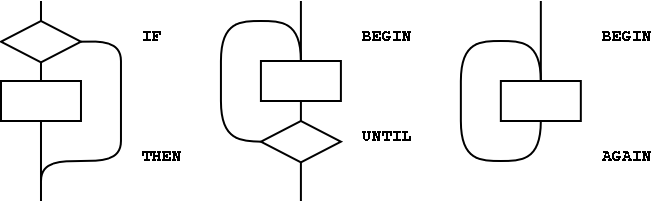
\includegraphics[bb=0 0 658 202,width=0.8\textwidth]{basic.png}}
	\caption{The basic control-flow patterns}
	\label{fig:basic}
  \end{center}
\end{figure}

In control flow every branch, or transfer of control, must terminate
at some destination. A natural implementation uses a stack to
remember the origin of forward branches and the destination of
backward branches. At a minimum, only the location of each origin or
destination must be indicated, although other implementation-dependent
information also may be maintained.

An origin is the location of the branch itself. A destination is
where control would continue if the branch were taken. A destination
is needed to resolve the branch address for each origin, and conversely,
if every control-flow path is completed no unused destinations can
remain.

With the addition of just three words (\word[tools]{AHEAD},
\word[tools]{CS-ROLL} and \word[tools]{CS-PICK}), the basic control-flow
words supply the primitives necessary to compile a variety of transportable
control structures. The abilities required are compilation of forward
and backward conditional and unconditional branches and compile-time
management of branch origins and destinations. \textbf{Table
\ref{table:control}} shows the desired behavior.

\begin{table}[ht]
  \begin{center}
	\caption{Compilation behavior of control-flow words}
	\label{table:control}
	\begin{tabular}{lccl}
	\hline\hline
	\multicolumn{4}{l}{at compile time,} \\
	word: & supplies: & resolves: & is used to: \\ \hline
	\word{IF}				& \emph{orig}	&				&
	mark origin of forward conditional branch \\
	\word{THEN}				&				& \emph{orig}	&
	resolve \word{IF} or \word[tools]{AHEAD} \\
	\word{BEGIN}			& \emph{dest}	&				&
	mark backward destination \\
	\word{AGAIN}			&				& \emph{dest}	&
	resolve with backward unconditional branch \\
	\word{UNTIL}			&				& \emph{dest}	&
	resolve with backward conditional branch \\
	\word[tools]{AHEAD}		& \emph{orig}	&				&
	mark origin of forward unconditional branch \\
	\word[tools]{CS-PICK}	&				&				&
	copy item on control-flow stack \\
	\word[tools]{CS-ROLL}	&				&				&
	reorder items on control-flow stack \\
	\hline\hline
	\end{tabular}
  \end{center}
\end{table}

The requirement that control-flow words are properly balanced by other
control-flow words makes reasonable the description of a compile-time
implementation-defined \emph{control-flow stack}. There is no
prescription as to how the control-flow stack is implemented, e.g.,
data stack, linked list, special array. Each element of the
control-flow stack mentioned above is the same size.

With these tools, the remaining basic control-structure elements,
shown in \textbf{figure \ref{fig:additional}}, can be defined. The
stack notation used here for immediate words is ( \emph{compilation
/ execution} ).

\begin{quote}\ttfamily
  \begin{tabbing}
	\tab \= \hspace{10em} \= \kill
	\+ \word{:} \word{WHILE}~ \word{p} dest -{}- orig dest / flag -{}- ) \\
		\word{bs} conditional exit from loops \\
		\word{POSTPONE} \word{IF}		\> \word{bs} conditional forward brach \\
	\-	1 \word[tools]{CS-ROLL}			\> \word{bs} keep dest on top \\
	\word{;} \word{IMMEDIATE} \\[2\parskip]

	\+	\word{:} \word{REPEAT}~ \word{p} orig dest -{}- / -{}- ) \\
		\word{bs} resolve a single WHILE and return to BEGIN \\
		\word{POSTPONE} \word{AGAIN}	\> \word{bs} uncond. backward branch to dest \\
	\-	\word{POSTPONE} \word{THEN}		\> \word{bs} resolve forward branch from orig \\
	\word{;} \word{IMMEDIATE} \\[2\parskip]

	\+ \word{:} \word{ELSE}~ \word{p} orig1 -{}- orig2 / -{}- ) \\
		\word{bs} resolve IF supplying alternate execution \\
		\word{POSTPONE} \word[tools]{AHEAD}	\> \word{bs} unconditional forward branch orig2 \\
		1 \word[tools]{CS-ROLL}				\> \word{bs} put orig1 back on top \\
	\-	\word{POSTPONE} \word{THEN}			\> \word{bs} resolve forward branch from orig1 \\
	\word{;} \word{IMMEDIATE}
  \end{tabbing}
\end{quote}

\begin{figure}[ht]
  \begin{center}
	\fbox{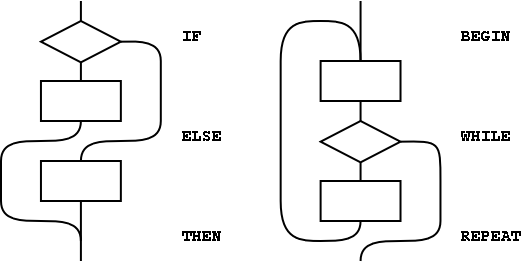
\includegraphics[bb=0 0 529 262,width=0.8\textwidth]{additional.png}}
	\caption{Additional basic control-flow patterns}
	\label{fig:additional}
  \end{center}
\end{figure}

Forth control flow provides a solution for well-known problems with
strictly structured programming.

The basic control structures can be supplemented, as shown in the
examples in \textbf{figure \ref{fig:extended}}, with additional
\word{WHILE}s in \word{BEGIN} {\ldots} \word{UNTIL} and \word{BEGIN}
{\ldots} \word{WHILE} {\ldots} \word{REPEAT} structures. However, for
each additional \word{WHILE} there must be a \word{THEN} at the end
of the structure. \word{THEN} completes the syntax with \word{WHILE}
and indicates where to continue execution when the \word{WHILE}
transfers control. The use of more than one additional \word{WHILE}
is possible but not common. Note that if the user finds this use of
\word{THEN} undesirable, an alias with a more likable name could be
defined.

Additional actions may be performed between the control flow word (the
\word{REPEAT} or \word{UNTIL}) and the \word{THEN} that matches the
additional \word{WHILE}. Further, if additional actions are desired
for normal termination and early termination, the alternative actions
may be separated by the ordinary Forth \word{ELSE}. The termination
actions are all specified after the body of the loop.

\begin{figure}[ht]
  \begin{center}
	\fbox{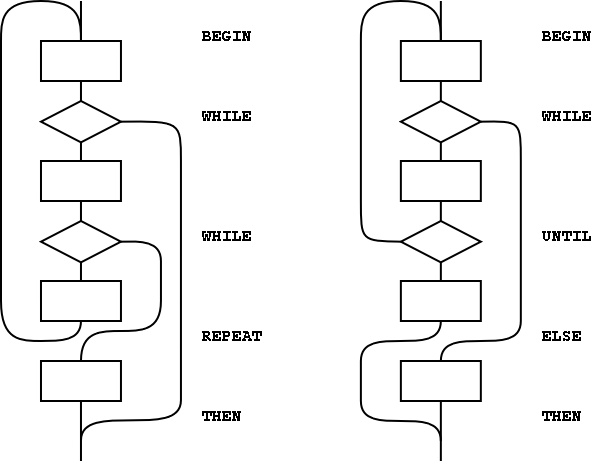
\includegraphics[bb=0 0 598 462, width=0.8\textwidth]{extended.png}}
	\caption{Extended control-flow patterns}
	\label{fig:extended}
  \end{center}
\end{figure}

Note that \word{REPEAT} creates an anomaly when matching the
\word{WHILE} with \word{ELSE} or \word{THEN}, most notably when
compared with the \word{BEGIN}{\ldots}\word{UNTIL} case. That is,
there will be one less \word{ELSE} or \word{THEN} than there are
\texttt{WHILE}s because \word{REPEAT} resolves one \word{THEN}. As
above, if the user finds this count mismatch undesirable, \word{REPEAT}
could be replaced in-line by its own definition.

Other loop-exit control-flow words, and even other loops, can be
defined. The only requirements are that the control-flow stack is
properly maintained and manipulated.

The simple implementation of the ANS Forth \word{CASE} structure
below is an example of control structure extension. Note the
maintenance of the data stack to prevent interference with the
possible control-flow stack usage.

\begin{quote}\ttfamily
  \begin{tabbing}
	\tab \= \hspace{10em} \= \kill
	0 \word{CONSTANT} \word{CASE} \word{IMMEDIATE}~ \word{p} init count of OFs ) \\[2\parskip]

	\+ \word{:} \word{OF}~ \word{p} \#of -{}- orig \#of+1 / x -{}- ) \\
		\word{1+}					\> \word{p} count OFs ) \\
		\word{toR}					\> \word{p} move off the stack in case the control-flow ) \\
									\> \word{p} stack is the data stack. ) \\
		\word{POSTPONE} \word{OVER}~ \word{POSTPONE} \word{=}~
								\word{p} copy and test case value) \\
		\word{POSTPONE} \word{IF}	\> \word{p} add orig to control flow stack ) \\
		\word{POSTPONE} \word{DROP}	\> \word{p} discards case value if = ) \\
	\-	\word{Rfrom}				\> \word{p} we can bring count back now ) \\
	\word{;} \word{IMMEDIATE} \\[2\parskip]

	\+ \word{:} \word{ENDOF}~ \word{p} orig1 \#of -{}- orig2 \#of ) \\
		\word{toR}					\> \word{p} move off the stack in case the control-flow ) \\
									\> \word{p} stack is the data stack. ) \\
		\word{POSTPONE} \word{ELSE} \\
	\-	\word{Rfrom}				\> \word{p} we can bring count back now ) \\
	\word{;} \word{IMMEDIATE} \\[2\parskip]

	\+ \word{:} \word{ENDCASE}~ \word{p} orig1..orign \#of -{}- ) \\
		\word{POSTPONE} \word{DROP}	\> \word{p} discard case value ) \\
		0 \word{qDO} \\
		\tab \word{POSTPONE} \word{THEN} \\
	\- \word{LOOP} \\
	\word{;} \word{IMMEDIATE}
  \end{tabbing}
\end{quote}


\paragraph{Return stack} ~ % A.3.2.3.3

The restrictions in section \xref[3.2.3.3 Return stack]{usage:returnstack}
are necessary if implementations are to be allowed to place loop
parameters on the return stack.

\addtocounter{subsubsection}{2}
\subsubsection{Environmental queries} % A.3.2.6

The size in address units of various data types may be determined by
phrases such as \texttt{1} \word{CHARS}. Similarly, alignment may be
determined by phrases such as \texttt{1} \word{ALIGNED}.

The environmental queries are divided into two groups: those that
always produce the same value and those that might not. The former
groups include entries such as \texttt{MAX-N}. This information is
fixed by the hardware or by the design of the Forth system; a user
is guaranteed that asking the question once is sufficient.

The other group of queries are for things that may legitimately
change over time. For example an application might test for the
presence of the Double Number word set using an environment query.
If it is missing, the system could invoke a system-dependent process
to load the word set. The system is permitted to change
\word{ENVIRONMENTq}'s database so that subsequent queries about it
indicate that it is present.

Note that a query that returns an ``unknown'' response could produce
a ``known'' result on a subsequent query.


\subsection{The Forth dictionary} % A.3.3

A Standard Program may redefine a standard word with a non-standard
definition. The program is still Standard (since it can be built on
any Standard System), but the effect is to make the combined entity
(Standard System plus Standard Program) a non-standard system.

\subsubsection{Name space} % A.3.3.1

\setcounter{paragraph}{1}
\paragraph{Definition names} ~ % A.3.3.1.2

The language in this section is there to ensure the portability of
Standard Programs. If a program uses something outside the Standard
that it does not provide itself, there is no guarantee that another
implementation will have what the program needs to run. There is no
intent whatsoever to imply that all Forth programs will be somehow
lacking or inferior because they are not standard; some of the finest
jewels of the programmer's art will be non-standard. At the same time,
the committee is trying to ensure that a program labeled ``Standard''
will meet certain expectations, particularly with regard to portability.

In many system environments the input source is unable to supply
certain non-graphic characters due to external factors, such as the
use of those characters for flow control or editing. In addition,
when interpreting from a text file, the parsing function specifically
treats non-graphic characters like spaces; thus words received by the
text interpreter will not contain embedded non-graphic characters. To
allow implementations in such environments to call themselves Standard,
this minor restriction on Standard Programs is necessary.

A Standard System is allowed to permit the creation of definition
names containing non-graphic characters. Historically, such names
were used for keyboard editing functions and ``invisible'' words.

\subsubsection{Code space} % A.3.3.2

\subsubsection{Data space} % A.3.3.3

The words \word{numTIB}, \word{toIN}, \word{BASE}, \word[block]{BLK},
\word[block]{SCR}, \word{SOURCE}, \word{SOURCE-ID}, \word{STATE}, and
\word{TIB} contain information used by the Forth system in its
operation and may be of use to the application. Any assumption made
by the application about data available in the Forth system it did
not store other than the data just listed is an environmental
dependency.

There is no point in specifying (in the Standard) both what is and
what is not addressable. A Standard Program may NOT address:

\begin{itemize}
\item Directly into the data or return stacks;
\item Into a definition's data field if not stored by the application.
\end{itemize}

The read-only restrictions arise because some Forth systems run from
ROM and some share I/O buffers with other users or systems. Portable
programs cannot know which areas are affected, hence the general
restrictions.

\paragraph{Address alignment} ~ % A.3.3.3.1

Many processors have restrictions on the addresses that can be used
by memory access instructions. For example, on a Motorola 68000,
16-bit or 32-bit data can be accessed only at even addresses. Other
examples include RISC architectures where 16-bit data can be loaded
or stored only at even addresses and 32-bit data only at addresses
that are multiples of four.

An implementor of ANS Forth can handle these alignment restrictions
in one of two ways. Forth's memory access words (\word{@}, \word{!},
\word{+!}, etc.) could be implemented in terms of smaller-width access
instructions which have no alignment restrictions. For example, on a
68000 Forth with 16-bit cells, \word{@} could be implemented with two
68000 byte-fetch instructions and a reassembly of the bytes into a
16-bit cell. Although this conceals hardware restrictions from the
programmer, it is inefficient, and may have unintended side effects
in some hardware environments. An alternate implementation of ANS Forth
could define each memory-access word using the native instructions
that most closely match the word's function. On a 68000 Forth with
16-bit cells, \word{@} would use the 68000's 16-bit move instruction.
In this case, responsibility for giving \word{@} a correctly-aligned
address falls on the programmer. A portable ANS Forth program must
assume that alignment may be required and follow the requirements of
this section.

\paragraph{Contiguous regions} ~ % A.3.3.3.2

The data space of a Forth system comes in discontinuous regions! The
location of some regions is provided by the system, some by the
program. Data space is contiguous within regions, allowing address
arithmetic to generate valid addresses only within a single region.
A Standard Program cannot make any assumptions about the relative
placement of multiple regions in memory.

Section \ref{usage:contiguous} does prescribe conditions under which
contiguous regions of data space may be obtained. For example:
\begin{quote}\ttfamily
	\word{CREATE} TABLE \quad
	1 \word{C,} 2 \word{C,} \word{ALIGN} 1000 \word{,} 2000 \word{,}
\end{quote}
makes a table whose address is returned by \texttt{TABLE}. In
accessing this table,
\begin{quote}
  \begin{tabular}{ll}
	\texttt{TABLE} \word{C@}					& will return 1 \\
	\texttt{TABLE} \word{CHAR+} \word{C@}		& will return 2 \\
	\texttt{TABLE} \texttt{2} \word{CHARS} \word{+}
		\word{ALIGNED} \word{@}					& will return 1000 \\
	\texttt{TABLE} \texttt{2} \word{CHARS} \word{+}
		\word{ALIGNED} \word{CELL+} \word{@}	&  will return 2000. \\
  \end{tabular}
\end{quote}
Similarly,
\begin{quote}\ttfamily
	\word{CREATE} DATA \quad 1000 \word{ALLOT}
\end{quote}
makes an array 1000 address units in size. A more portable strategy
would define the array in application units, such as:
\begin{quote}\ttfamily
	500 \word{CONSTANT} NCELLS \\
	\word{CREATE} CELL-DATA NCELLS \word{CELLS} \word{ALLOT}
\end{quote}

This array can be indexed like this:
\begin{quote}\ttfamily
	\word{:} LOOK \quad
		NCELLS 0 \word{DO}
			CELL-DATA \word{I} \word{CELLS} \word{+} \word[tools]{q}
		\word{LOOP}
	\word{;}
\end{quote}


\setcounter{paragraph}{5}
\paragraph{Other transient regions} ~ % A.3.3.3.6

In many existing Forth systems, these areas are at \word{HERE} or
just beyond it, hence the many restrictions.

$(2*n)+2$ is the size of a character string containing the
unpunctuated binary representation of the maximum double number with
a leading minus sign and a trailing space.

Implementation note: Since the minimum value of \param{n} is 16, the
absolute minimum size of the pictured numeric output string is 34
characters. But if your implementation has a larger \param{n}, you must
also increase the size of the pictured numeric output string.

\subsection{The Forth text interpreter} % A.3.4

\setcounter{subsubsection}{1}
\setcounter{paragraph}{2}
\paragraph{Numeric notation} ~% A.3.4.1.3
\label{rat:notation:numeric}

The numeric representation provided by the \textsf{X:number-prefix}
extension can be tested with the following test cases:

\begin{tt}
	\word{DECIMAL} \\
	\{ \#1289       -> 1289        \} \\
	\{ \#12346789.  -> 12346789.   \} \\
	\{ \#-1289      -> -1289       \} \\
	\{ \#-12346789. -> -12346789.  \} \\
	\{ \$12eF       -> 4847        \} \\
	\{ \$12aBcDeF.  -> 313249263.  \} \\
	\{ \$-12eF      -> -4847       \} \\
	\{ \$-12AbCdEf. -> -313249263. \} \\
	\{ \%10010110   -> 150         \} \\
	\{ \%10010110.  -> 150.        \} \\
	\{ \%-10010110  -> -150        \} \\
	\{ \%-10010110. -> -150.       \} \\
	\{ 'z'          -> 122         \}
\end{tt}

\setcounter{subsubsection}{2}
\subsubsection{Semantics} % A.3.4.3

The ``initiation semantics'' correspond to the code that is executed
upon entering a definition, analogous to the code executed by
\word{EXIT} upon leaving a definition. The ``run-time semantics''
correspond to code fragments, such as literals or branches, that are
compiled inside colon definitions by words with explicit compilation
semantics.

In a Forth cross-compiler, the execution semantics may be specified
to occur in the host system only, the target system only, or in both
systems. For example, it may be appropriate for words such as
\word{CELLS} to execute on the host system returning a value describing
the target, for colon definitions to execute only on the target, and
for \word{CONSTANT} and \word{VARIABLE} to have execution behaviors on
both systems. Details of cross-compiler behavior are beyond the scope
of this Standard.

\setcounter{paragraph}{1}
\paragraph{Interpretation semantics} ~ % A.3.4.3.2
\label{rat:interpret}

For a variety of reasons, this Standard does not define interpretation
semantics for every word. Examples of these words are \word{toR},
\word{.q}, \word{DO}, and \word{IF}. Nothing in this Standard precludes
an implementation from providing interpretation semantics for these
words, such as interactive control-flow words. However, a Standard
Program may not use them in interpretation state.

\addtocounter{subsubsection}{1}
\subsubsection{Compilation} % A.3.4.5

Compiler recursion at the definition level consumes excessive
resources, especially to support locals. The Technical Committee
does not believe that the benefits justify the costs. Nesting
definitions is also not common practice and won't work on many
systems.

\section{Documentation requirements} % A.4 ==========================

\subsection{System documentation} % A.4.1

\subsection{Program documentation} % A.4.2

\section{Compliance and labeling} % A.5 =============================

\subsection{ANS Forth systems} % A.5.1

Section \ref{label:label} defines the criteria that a system must
meet in order to justify the label ``ANS Forth System''. Briefly,
the minimum requirement is that the system must ``implement'' the
Core word set. There are several ways in which this requirement may
be met. The most obvious is that all Core words may be in a pre-compiled
kernel. This is not the only way of satisfying the requirement,
however. For example, some words may be provided in source blocks or
files with instructions explaining how to add them to the system if
they are needed. So long as the words are provided in such a way that
the user can obtain access to them with a clear and straightforward
procedure, they may be considered to be present.

A Forth cross-compiler has many characteristics in common with an ANS
Forth System, in that both use similar compiling tools to process a
program. However, in order to fully specify an ANS Forth cross compiler
it would be necessary to address complex issues dealing with compilation
and execution semantics in both host and target environments as well as
ROMability issues. The level of effort to do this properly has proved to
be impractical at this time. As a result, although it may be possible
for a Forth cross-compiler to correctly prepare an ANS Forth program
for execution in a target environment, it is inappropriate for a
cross-compiler to be labeled an ANS Forth System.

\subsection{ANS Forth programs} % A.5.2

\setcounter{subsubsection}{1}
\subsubsection{Program labeling} % A.5.2.2

Declaring an environmental dependency should not be considered
undesirable, merely an acknowledgment that the author has taken
advantage of some assumed architecture. For example, most computers
in common use are based on two's complement binary arithmetic. By
acknowledging an environmental dependency on this architecture,
a programmer becomes entitled to use the number \texttt{-1} to
represent all bits set without significantly restricting the
portability of the program.

Because all programs require space for data and instructions, and
time to execute those instructions, they depend on the presence of
an environment providing those resources. It is impossible to predict
how little of some of these resources (e.g. stack space) might be
necessary to perform some task, so this Standard does not do so.

On the other hand, as a program requires increasing levels of
resources, there will probably be sucessively fewer systems on
which it will execute sucessfully. An algorithm requiring an array
of $10^9$ cells might run on fewer computers than one requiring
only $10^3$.

Since there is also no way of knowing what minimum level of resources
will be implemented in a system useful for at least some tasks, any
program performing real work labeled simply an ``ANS Forth Program''
is unlikely to be labeled correctly.


\section{Glossary} % A.6 ============================================

In this and following sections we present rationales for the handling
of specific words: why we included them, why we placed them in certain
word sets, or why we specified their names or meaning as we did.

Words in this section are organized by word set, retaining their index
numbers for easy cross-referencing to the glossary.

Historically, many Forth systems have been written in Forth. Many of
the words in Forth originally had as their primary purpose support of
the Forth system itself. For example, \word{WORD} and \word{FIND} are
often used as the principle instruments of the Forth text interpreter,
and \word{CREATE} in many systems is the primitive for building
dictionary entries. In defining words such as these in a standard way,
we have endeavored not to do so in such a way as to preclude their use
by implementors. One of the features of Forth that has endeared it to
its users is that the same tools that are used to implement the system
are available to the application programmer --- a result of this
approach is the compactness and efficiency that characterizes most
Forth implementations.

\readrationale{core}


\setcounter{subsection}{1}
\subsection{Core extension words} % A.6.2 =================

The words in this collection fall into several categories:

\begin{itemize}
\item Words that are in common use but are deemed less essential than
	Core words (e.g., \word{0ne});

\item Words that are in common use but can be trivially defined from
	Core words (e.g., \word{FALSE});

\item Words that are primarily useful in narrowly defined types of
	applications or are in less frequent use (e.g., \word{PARSE});

\item Words that are being deprecated in favor of new words introduced
	to solve specific problems (e.g., \word{CONVERT}).
\end{itemize}

Because of the varied justifications for inclusion of these words,
the Technical Committee does not encourage implementors to offer the
complete collection, but to select those words deemed most valuable to
their clientele.

\readrationale{core-ext}


\section{The optional Block word set} % A.7 =========================
\setwordlist{block}
\label{rat:block}

Early Forth systems ran stand-alone, with no host OS. Blocks of 1024
bytes were designed as a convenient unit of disk, and most native
Forth systems still use them. It is relatively easy to write a native
disk driver that maps head/track/sector addresses to block numbers.
Such disk drivers are extremely fast in comparison with conventional
file-oriented operating systems, and security is high because there is
no reliance on a disk map.

Today many Forth implementations run under host operating systems,
because the compatibility they offer the user outweighs the performance
overhead. Many people who use such systems prefer using host OS files
only; however, people who use both native and non-native Forths need a
compatible way of accessing disk. The Block Word set includes the most
common words for accessing program source and data on disk.

In order to guarantee that Standard Programs that need access to mass
storage have a mechanism appropriate for both native and non-native
implementations, ANS Forth requires that the Block word set be
available if any mass storage facilities are provided. On non-native
implementations, blocks normally reside in host OS files.

\setcounter{subsection}{1}
\subsection{Additional terms} % A.7.2 ===============================

\begin{description}
\item[block] ~

	Many Forth systems use blocks to contain program source.
	Conventionally such blocks are formatted for editing as
	16 lines of 64 characters. Source blocks are often referred
	to as ``screens''.
\end{description}

\setcounter{subsection}{5}
\subsection{Glossary} % A.7.6 =============================

\readrationale{block}


\section{The optional Double-Number word set} % A.8 =================
\setwordlist{double}
\label{rat:double}

Forth systems on 8-bit and 16-bit processors often find it necessary
to deal with double-length numbers. But many Forths on small embedded
systems do not, and many users of Forth on systems with a cell size of
32-bits or more find that the necessity for double-length numbers is
much diminished. Therefore, we have factored the words that manipulate
double-length entities into this optional word set.

Please note that the naming convention used in this word set conveys
some important information:

\begin{enumerate}
\item[1.]
	Words whose names are of the form \texttt{2}\emph{xxx} deal
	with cell pairs, where the relationship between the cells is
	unspecified. They may be two-vectors, double-length numbers, or
	any pair of cells that it is convenient to manipulate together.

\item[2.]
	Words with names of the form \texttt{D}\emph{xxx} deal
	specifically with double-length integers.

\item[3.]
	Words with names of the form \texttt{M}\emph{xxx} deal with
	some combination of single and double integers. The order in
	which these appear on the stack is determined by long-standing
	common practice.
\end{enumerate}

Refer to \ref{rat:types} for a discussion of data types in Forth.

\setcounter{subsection}{5}
\subsection{Glossary} % A.8.6 =============================

\readrationale{double}


\section{The optional Exception word set} % A.9 =====================
\setwordlist{exception}
\label{rat:exception}

\word{CATCH} and \word{THROW} provide a reliable mechanism for
handling exceptions, without having to propagate exception flags
through multiple levels of word nesting. It is similar in spirit
to the ``non-local return'' mechanisms of many other languages,
such as C's \texttt{setjmp()} and \texttt{longjmp()}, and LISP's
\texttt{CATCH} and \texttt{THROW}. In the Forth context, \word{THROW}
may be described as a ``multi-level \word[core]{EXIT}'', with
\word{CATCH} marking a location to which a \word{THROW} may return.

Several similar Forth ``multi-level \word[core]{EXIT}''
exception-handling schemes have been described and used in past years.
It is not possible to implement such a scheme using only standard words
(other than \word{CATCH} and \word{THROW}), because there is no portable
way to ``unwind'' the return stack to a predetermined place.

\word{THROW} also provides a convenient implementation technique for
the standard words \word{ABORT} and \word{ABORTq}, allowing an
application to define, through the use of \word{CATCH}, the behavior
in the event of a system \word{ABORT}.

This sample implementation of \word{CATCH} and \word{THROW} uses the
non-standard words described below.  They or their equivalents are
available in many systems.  Other implementation strategies, including
directly saving the value of \word[core]{DEPTH}, are possible if such
words are not available.

\begin{quote}
\texttt{SP@} \stack{}{addr}
	returns the address corresponding to the top of data stack.

\texttt{SP!} \stack{addr}{}
	sets the stack pointer to \emph{addr}, thus restoring the stack
	depth to the same depth that existed just before \emph{addr} was
	acquired by executing \texttt{SP@}.

\texttt{RP@} \stack{}{addr}
	returns the address corresponding to the top of return stack.

\texttt{RP!} \stack{addr}{}
	sets the return stack pointer to \emph{addr}, thus restoring the
	return stack depth to the same depth that existed just before
	\emph{addr} was acquired by executing \texttt{RP@}.

	\ttfamily
	\begin{tabbing}
	\tab \= \tab \= \hspace{7em} \= ( saved-sp ) \= \kill
	\word{VARIABLE} HANDLER ~ 0 HANDLER \word{!} ~ \word{bs} last exception handler \\[\parskip]

	\+ \word{:} \word{CATCH} ~ \word{p} xt -{}- exception\# | 0 ) \word{bs} return addr on stack \\
		SP@ \word{toR}				\>\> \word{p} xt )	\> \word{bs} save data stack pointer \\
		HANDLER \word{@} \word{toR}	\>\> \word{p} xt )	\> \word{bs} and previous handler \\
		RP@ HANDLER \word{!}		\>\> \word{p} xt )	\> \word{bs} set current handler \\
		\word{EXECUTE}				\>\> \word{p} )		\> \word{bs} execute returns if no THROW \\
		\word{Rfrom} HANDLER \word{!}	\>\> \word{p} )		\> \word{bs} restore previous handler \\
		\word{Rfrom} \word{DROP}		\>\> \word{p} )		\> \word{bs} discard saved stack ptr \\
	\-	0							\>\> \word{p} 0 )	\> \word{bs} normal completion \\
	\word{;} \\[\parskip]

	\+ \word{:} \word{THROW} \word{p} ??? exception\# -{}- ??? exception\# ) \\
		\+ \word{qDUP} \word{IF}			\>\> \word{p} exc\# )	\> \word{bs} 0 THROW is no-op \\
			HANDLER \word{@} RP!			\> \word{p} exc\# ) \> \word{bs} restore prev return stack \\
			\word{Rfrom} HANDLER \word{!}		\> \word{p} exc\# ) \> \word{bs} restore prev handler \\
			\word{Rfrom} \word{SWAP} \word{toR} \> \word{p} saved-sp ) \> \word{bs} exc\# on return stack \\
			SP! \word{DROP} \word{Rfrom}		\> \word{p} exc\# ) 	\> \word{bs} restore stack \\
			\word{bs} Return to the caller of CATCH because return \\
			\word{bs} stack is restored to the state that existed \\
		\-	\word{bs} when CATCH began execution \\
	\- \word{THEN} \\
	\word{;}
	\end{tabbing}
\end{quote}

In a multi-tasking system, the \texttt{HANDLER} variable should be in
the per-task variable area (i.e., a user variable).

This sample implementation does not explicitly handle the case in
which \word{CATCH} has never been called (i.e., the \word{ABORT}
behavior). One solution is to add the following code after the
\word{IF} in \word{THROW}:
\begin{quote}\ttfamily
	HANDLER \word{@} \word{0=} \word{IF}
		\word{p} empty the stack ) \word{QUIT}
	\word{THEN}
\end{quote}
Another solution is to execute \word{CATCH} within \word{QUIT}, so
that there is always an ``exception handler of last resort'' present.
For example:
\begin{quote}\ttfamily
	\word{:} \word{QUIT} \\
	\tab \word{p} empty the return stack and ) \\
	\tab \word{p} set the input source to the user input device )\\
	\tab \word{POSTPONE} \word{[} \\
	\tab \word{BEGIN} \\
	\tab~~ \word{REFILL} \\
	\tab \word{WHILE} \\
	\tab~~ \word{[']} INTERPRET ~ \word{CATCH}\\
	\tab~~ \word{CASE} \\
	\tab\tab ~0 \word{OF} \word{STATE} \word{@} \word{0=} \word{IF}
		\word{.q} OK" \word{THEN} \word{CR} ~\word{ENDOF} \\
	\tab\tab -1 \word{OF} \word{p} Aborted) \word{ENDOF} \\
	\tab\tab -2 \word{OF} \word{p} display message from \word{ABORTq} ) \word{ENDOF} \\
	\tab\tab \word{p} default ) \word{DUP} \word{.q} Exception \# " ~ \word{d} \\
	\tab~~ \word{ENDCASE} \\
	\tab \word{REPEAT} \word[tools]{BYE} \\
	\word{;}
\end{quote}

This example assumes the existance of a system-implementation word
\texttt{INTERPRET} that embodies the text interpreter semantics
described in \xref[3.4 The Forth text interpreter]{usage:command}.
Note that this implementation of \word{QUIT} automatically handles
the emptying of the stack and return stack, due to
\word{THROW}'s inherent restoration of the data and return
stacks. Given this definition of \word{QUIT}, it's easy to define:

\tab \word{:} \word{ABORT}
	\texttt{-1} \word{THROW}
\word{;}

In systems with other stacks in addition to the data and return stacks,
the implementation of \word{CATCH} and \word{THROW} must save and
restore those stack pointers as well. Such an ``extended version'' can
be built on top of this basic implementation. For example, with another
stack pointer accessed with \texttt{FP@} and \texttt{FP!} only
\word{CATCH} needs to be redefined:

\begin{quote}\ttfamily
	\word{:} \word{CATCH}
		\word{p} \texttt{xt -{}- exception\# | 0 )} \\
	\tab FP@ \word{toR} \word{CATCH} \word{Rfrom}
		\word{OVER} \word{IF} FP! \word{ELSE} \word{DROP} \word{THEN}
	\word{;}
\end{quote}

No change to \word{THROW} is necessary in this case. Note that, as
with all redefinitions, the redefined version of \word{CATCH} will
only be available to definitions compiled after the redefinition of
\word{CATCH}.

\word{CATCH} and \word{THROW} provide a convenient way for an
implementation to ``clean up'' the state of open files if an
exception occurs during the text interpretation of a file with
\word[file]{INCLUDE-FILE}. The implementation of
\word[file]{INCLUDE-FILE} may guard (with \word{CATCH}) the word
that performs the text interpretation, and if \word{CATCH} returns
an exception code, the file may be closed and the exception
re\word{THROW}n so that the files being included at an outer nesting
level may be closed also. Note that the Standard allows, but does not
require, \word[file]{INCLUDE-FILE} to close its open files if an
exception occurs. However, it does require \word[file]{INCLUDE-FILE}
to unnest the input source specification if an exception is
\word{THROW}n.

\setcounter{subsection}{2}
\subsection{Additional usage requirements} % A.9.3 ========

One important use of an exception handler is to maintain program
control under many conditions which \word{ABORT}.  This is practicable
only if a range of codes is reserved.  Note that an application may
overload many standard words in such a way as to \word{THROW}
ambiguous conditions not normally \word{THROW}n by a particular
system.

\setcounter{subsubsection}{5}
\subsubsection{Exception handling} % A.9.3.6 ==============

The method of accomplishing this coupling is implementation dependent.
For example, \word[block]{LOAD} could ``know'' about \word{CATCH} and
\word{THROW} (by using \word{CATCH} itself, for example), or
\word{CATCH} and \word{THROW} could ``know'' about \word[block]{LOAD}
(by maintaining input source nesting information in a data structure
known to \word{THROW}, for example). Under these circumstances it is
not possible for a Standard Program to define words such as
\word[block]{LOAD} in a completely portable way.

\setcounter{subsection}{5}
\subsection{Glossary} % A.9.6 =============================

\readrationale{exception}


\section{The optional Facility word set} % A.10 =====================
\setwordlist{facility}
\label{rat:facility}

\setcounter{subsection}{5}
\subsection{Glossary} % A.10.6 ============================

\readrationale{facility}


\section{The optional File-Access word set} % A.11 ==================
\setwordlist{file}
\label{rat:file}

Many Forth systems support access to a host file system, and many of
these support interpretation of Forth from source text files.  The
Forth-83 Standard did not address host OS files.  Nevertheless, a
degree of similarity exists among modern implementations.

For example, files must be opened and closed, created and deleted.
Forth file-system implementations differ mostly in the treatment and
disposition of the exception codes, and in the format of the
file-identification strings.  The underlying mechanism for creating
file-control blocks might or might not be visible.  We have chosen to
keep it invisible.

Files must also be read and written. Text files, if supported, must
be read and written one line at a time. Interpretation of text files
implies that they are somehow integrated into the text interpreter
input mechanism.  These and other requirements have shaped the
file-access extensions word set.

Most of the existing implementations studied use simple English words
for common host file functions: \texttt{OPEN}, \texttt{CLOSE},
\texttt{READ}, etc.  Although we would have preferred to do likewise,
there were so many minor variations in implementation of these words
that adopting any particular meaning would have broken much existing
code.  We have used names with a suffix \texttt{-FILE} for most of these
words.  We encourage implementors to conform their single-word primitives
to the ANS behaviors, and hope that if this is done on a widespread
basis we can adopt better definition names in a future standard.

Specific rationales for members of this word set follow.

\setcounter{subsection}{2}
\subsection{Additional usage requirements} % A.11.3 =======

\setcounter{subsubsection}{1}
\subsubsection{Blocks in files} % 11.3.2 ==================

Many systems reuse file identifiers; when a file is closed, a
subsequently opened file may be given the same identifier. If the
original file has blocks still in block buffers, these will be
incorrectly associated with the newly opened file with disastrous
results. The block buffer system must be flushed to avoid this.

\setcounter{subsection}{5}
\subsection{Glossary} % A.11.6 ============================

\readrationale{file}


\section{The optional Floating-Point word set} % A.12 ===============
\setwordlist{floating}
\label{rat:floating}

The Technical Committee has considered many proposals dealing with
the inclusion and makeup of the Floating-Point Word Sets in ANS
Forth. Although it has been argued that ANS Forth should not address
floating-point arithmetic and numerous Forth applications do not need
floating-point, there are a growing number of important Forth
applications from spread sheets to scientific computations that
require the use of floating-point arithmetic. Initially the Technical
Committee adopted proposals that made the \emph{Forth Vendors Group
Floating-Point Standard}, first published in 1984, the framework for
inclusion of Floating-Point in ANS Forth. There is substantial common
practice and experience with the Forth Vendors Group Floating-Point
Standard.  Subsequently the Technical Committee adopted proposals that
placed the basic floating-point arithmetic, stack and support words
in the Floating-Point word set and the floating-point transcendental
functions in the Floating-Point Extensions word set. The Technical
Committee also adopted proposals that:

\begin{itemize}
\item changed names for clarity and consistency; e.g.,
	\texttt{REALS} to \word{FLOATS}, and
	\texttt{REAL+} to \word{FLOAT+}.
\item removed words; e.g., \texttt{FPICK}.
\item added words for completeness and increased functionality; e.g.,
	\word{FSINCOS},
	\word{Ftilde},
	\word{DF@},
	\word{DF!},
	\word{SF@} and
	\word{SF!}
\end{itemize}

Several issues concerning the Floating-Point word set were resolved
by consensus in the Technical Committee:

\begin{description}
\item [Floating-point stack:]
	By default the floating-point stack is separate from the data
	and return stacks; however, an implementation may keep
	floating-point numbers on the data stack. A program can determine
	whether floating-point numbers are kept on the data stack by
	passing the string \texttt{FLOATING-STACK} to \word{ENVIRONMENTq}
	It is the experience of several members of the Technical Committee
	that with proper coding practices it is possible to write
	floating-point code that will run identically on systems with a
	separate floating-point stack and with floating-point numbers kept
	on the data stack.

\item[Floating-point input:]
	The current base must be \word{DECIMAL}. Floating-point input
	is not allowed in an arbitrary base. All floating-point numbers to
	be interpreted by an ANS Forth system must contain the exponent
	indicator ``\texttt{E}'' (see \xref[12.3.7 Text	interpreter input
	number conversion]{float:conv}). Consensus in the Technical
	Committee deemed this form of floating-point input to be in more
	common use than the alternative that would have a floating-point
	input mode that would allow numbers with embedded decimal points
	to be treated as floating-point numbers.

\item[Floating-point representation:]
	Although the format and precision of the significand and the format
	and range of the exponent of a floating-point number are
	implementation defined in ANS Forth, the Floating-Point Extensions
	word set contains the words
	\word{DF@}, \word{SF@}, \word{DF!}, and \word{SF!}
	for fetching and storing double- and single-precision IEEE
	floating-point-format numbers to memory. The IEEE floating-point
	format is commonly used by numeric math co-processors and for
	exchange of floating-point data between programs and systems.
\end{description}

\setcounter{subsection}{2}
\subsection{Additional usage requirements} % A.12.3 =======

\setcounter{subsubsection}{4}
\subsubsection{Address alignment} % A.12.3.5 ==============

In defining custom floating-point data structures, be aware that
\word{CREATE} doesn't necessarily leave the data space pointer
aligned for various floating-point data types. Programs may comply
with the requirement for the various kinds of floating-point alignment
by specifying the appropriate alignment both at compile-time and
execution time. For example:

\begin{quote}\ttfamily
	\word{:} \word{FCONSTANT} \word{p} F: r -{}- ) \\
	\tab \word{CREATE} \word{FALIGN} ~\word{HERE}~
		1 \word{FLOATS} \word{ALLOT} ~\word{F!} \\
	\tab \word{DOES} \word{p} F: -{}- r )
		~\word{FALIGNED} \word{F@} \word{;}
\end{quote}

\setcounter{subsubsection}{6}
\subsubsection{Text interpreter input number conversion} % A.12.3.7

The Technical Committee has more than once received the suggestion
that the text interpreter in Standard Forth systems should treat
numbers that have an embedded decimal point, but no exponent, as
floating-point numbers rather than double cell numbers. This
suggestion, although it has merit, has always been voted down because
it would break too much existing code; many existing implementations
put the full digit string on the stack as a double number and use
other means to inform the application of the location of the decimal
point.

\setcounter{subsection}{5}
\subsection{Glossary} % A.12.6 ============================

\readrationale{floating}


\section{The optional Locals word set} % A.13 =======================
\setwordlist{local}
\label{rat:local}

The Technical Committee has had a problem with locals. It has been
argued forcefully that ANS Forth should say nothing about locals
since:

\begin{itemize}
\item there is no clear accepted practice in this area;
\item not all Forth programmers use them or even know what they are;
	and
\item few implementations use the same syntax, let alone the same
	broad usage rules and general approaches.
\end{itemize}

It has also been argued, it would seem equally forcefully, that the
lack of any standard approach to locals is precisely the reason for
this lack of accepted practice since locals are at best non-trivial
to implement in a portable and useful way. It has been further argued
that users who have elected to become dependent on locals tend to be
locked into a single vendor and have little motivation to join the
group that it is hoped will ``broadly accept'' ANS Forth unless the
Standard addresses their problems.

Since the Technical Committee has been unable to reach a strong
consensus on either leaving locals out or on adopting any particular
vendor's syntax, it has sought some way to deal with an issue that it
has been unable to simply dismiss. Realizing that no single mechanism
or syntax can simultaneously meet the desires expressed in all the
locals proposals that have been received, it has simplified the
problem statement to be to define a locals mechanism that:

\begin{itemize}
\item is independent of any particular syntax;
\item is user extensible;
\item enables use of arbitrary identifiers,
	local in scope to a single definition;
\item supports the fundamental cell size data types of Forth;
	and
\item works consistently, especially with respect to
	re-entrancy and recursion.
\end{itemize}

This appears to the Technical Committee to be what most of those who
actively use locals are trying to achieve with them, and it is at
present the consensus of the Technical Committee that if ANS Forth has
anything to say on the subject this is an acceptable thing for it to
say.

This approach, defining \word{LOCAL}, is proposed as one that can be
used with a small amount of user coding to implement some, but not all,
of the locals schemes in use. The following coding examples illustrate
how it can be used to implement two syntaxes.

\begin{itemize}
\item The syntax defined by this Standard and used in the systems of
	Creative Solutions, Inc.:

	\begin{quote}\ttfamily
	\word{:} \word{LOCALS} \word{p} "name{\ldots}name |" -{}- ) \\
	\tab \word{BEGIN} \\
	\tab~ \word{BL} \word{WORD} ~ \word{COUNT} \word{OVER} \word{C@} \\
	\tab~ \word{[CHAR]} | \word{-} \word{OVER} 1 \word{-} \word{OR} ~ \word{WHILE} \\
	\tab~ \word[local]{LOCAL} \\
	\tab \word{REPEAT} \word{2DROP} ~ 0 0 \word{LOCAL} \\
	\word{;} \word{IMMEDIATE}

	\word{:} EXAMPLE \word{p} n -{}- n**2 n**3 ) \\
	\tab \word{LOCALS} N |
		~ N \word{DUP} N \word{*} ~\word{DUP} N \word{*}
	\word{;}
	\end{quote}

\item A proposed syntax: ( \texttt{LOCAL} \emph{name} ) with
	additional usage rules:

	\begin{quote}\ttfamily
	\word{:} LOCAL \word{p} "name" -{}- )
		\word{BL} \word{WORD} \word{COUNT} \word{LOCAL}
	\word{;} ~\word{IMMEDIATE}

	\word{:} END-LOCALS \word{p} -{}- ) ~ 0 0 \word{LOCAL}
	\word{;} ~\word{IMMEDIATE}

	\word{:} EXAMPLE \word{p} n -{}- n n**2 n**3 ) \\
	\tab LOCAL N ~END-LOCALS ~
		N \word{DUP} N \word{*} ~ \word{DUP} N \word{*}
	\word{;}
	\end{quote}
\end{itemize}

Other syntaxes can be implemented, although some will admittedly
require considerably greater effort or in some cases program
conversion. Yet other approaches to locals are completely incompatible
due to gross differences in usage rules and in some cases even scope
identifiers. For example, the complete local scheme in use at Johns
Hopkins had elaborate semantics that cannot be duplicated in terms of
this model.

To reinforce the intent of section \ref{wordlist:local}, here are
two examples of actual use of locals. The first illustrates correct
usage:

\begin{enumerate}
\item[a)] \begin{quote}\ttfamily
	\word{:} \{	\word{p} "name {\ldots} \}" -{}- ) \\
	\tab \word{BEGIN} ~\word{BL} \word{WORD} \word{COUNT} \\
	\tab~~ \word{OVER} \word{C@} \word{[CHAR]} \} \word{-} ~
		\word{OVER} 1 \word{-} ~
		\word{OR} \word{WHILE} \\
	\tab~~ \word{LOCAL} \\
	\tab \word{REPEAT} \word{2DROP} 0 0 \word{LOCAL}\\
	\word{;} \word{IMMEDIATE}
	\end{quote}

\item[b)] \begin{quote}\ttfamily
	\word{:} JOE \word{p} a b c -{}- n ) \\
	\tab \word{toR} \word{2*} \word{Rfrom} \word{2DUP} \word{+} 0 \\
	\tab \{ ANS 2B+C C 2B A \} \\
	\tab 2 0 \word{DO}
		~1 ANS \word{+} \word{I} \word{+} \word{TO} ANS
		~ANS \word{d} \word{CR}
	~\word{LOOP} \\
	\tab ANS \word{d} 2B+C \word{d} C \word{d} 2B \word{d} A \word{d} \word{CR} ANS \\
	\word{;}
	\end{quote}

\item[c)] \begin{quote}\ttfamily
	100 300 10 JOE \word{d}
	\end{quote}
\end{enumerate}

The word \texttt{\{} at a) defines a local declaration syntax that
surrounds the list of locals with braces. It doesn't do anything fancy,
such as reordering locals or providing initial values for some of them,
so locals are initialized from the stack in the default order. The
definition of \texttt{JOE} at b) illustrates a use of this syntax. Note
that work is performed at execution time in that definition before
locals are declared. It's OK to use the return stack as long as whatever
is placed there is removed before the declarations begin.

Note that before declaring locals, \texttt{B} is doubled, a
subexpression (\texttt{2B+C}) is computed, and an initial value (zero)
for \texttt{ANS} is provided. After locals have been declared,
\texttt{JOE} proceeds to use them. Note that locals may be accessed and
updated within do-loops. The effect of interpreting line c) is to
display the following values:

\begin{quote}
	\texttt{1} (\texttt{ANS} the first time through the loop),\\
	\texttt{3} (\texttt{ANS} the second time), \\
	\texttt{3} (\texttt{ANS}),
		\texttt{610} (\texttt{2B+C}),
		\texttt{10}  (\texttt{C}),
		\texttt{600} (\texttt{2B}),
		\texttt{100} (\texttt{A}), and \\
	\texttt{3} (\texttt{ANS} left on the stack by \texttt{JOE}).
\end{quote}

The \emph{names} of the locals vanish after \texttt{JOE} has been
compiled.  The \emph{storage and meaning} of locals appear when
\texttt{JOE}'s locals are declared and vanish as \texttt{JOE} returns
to its caller at \word{;} (semicolon).

A second set of examples illustrates various things that break the
rules.  We assume that the definitions of \texttt{LOCAL} and
\texttt{END-LOCALS} above are present, along with \texttt{\{} from
the preceding example.

\begin{enumerate}
\item[d)] \begin{quote}\ttfamily
	\word{:} ZERO ~ 0 \word{POSTPONE} \word{LITERAL} \word{POSTPONE} LOCAL
	\word{;} \word{IMMEDIATE}
	\end{quote}

\item[e)] \begin{quote}\ttfamily
	\word{:} MOE ~\word{p} a b ) \\
	\tab ZERO TEMP ~LOCAL B ~\word{1+} LOCAL A+ ~ZERO ANSWER \word{;}
	\end{quote}

\item[f)] \begin{quote}\ttfamily
	\word{:} BOB~ \word{p} a b c d ) ~\{ D C \} ~\{ B A \} \word{;}
	\end{quote}
\end{enumerate}

Here are two definitions with various violations of rule
\ref{locals:rules}a. In e) the declaration of \texttt{TEMP} is legal
and creates a local whose initial value is zero. It's OK because the
executable code that \texttt{ZERO} generates precedes the first use of
\word[local]{LOCAL} in the definition. However, the \word{1+}
preceding the declaration of \texttt{A+} is illegal. Likewise the use
of \texttt{ZERO} to define \texttt{ANSWER} is illegal because it
generates executable code between uses of \word{LOCAL}.
Finally, \texttt{MOE} terminates illegally (no \texttt{END-LOCALS}).
\texttt{BOB} in f) violates the rule against declaring two sets of
locals.
% \replace[1]{inf) violates}{inviolate}

\begin{enumerate}
\item[g)] \begin{quote}\ttfamily
	\word{:} ANN \word{p} a b -{}- b )
		\word{DUP} \word{toR} \word{DUP} \word{IF}
		\{ B A \} \word{THEN} \word{Rfrom} \word{;}
	\end{quote}

\item[h)] \begin{quote}\ttfamily
	\word{:} JANE \word{p} a b -{}- n )
		\{ B A \} A B \word{+} \word{toR} A B \word{-} ~\word{Rfrom} \word{/} \word{;}
	\end{quote}
\end{enumerate}

\texttt{ANN} in g) violates two rules. The \word{IF} {\ldots} \word{THEN}
around the declaration of its locals violates \ref{locals:rules}b, and
the copy of \texttt{B} left on the return stack before declaring locals
violates \ref{locals:rules}c. \texttt{JANE} in h) violates
\ref{locals:rules}d by accessing locals after placing the sum of
\texttt{A} and \texttt{B} on the return stack without first removing
that sum.

\begin{enumerate}
\item[i)] \begin{quote}\ttfamily
	\word{:} CHRIS \word{p} a b) \\
	\tab \{ B A \} \word{[']} A \word{EXECUTE}
		~5 \word{[']} B \word{toBODY} \word{!}
		~\word{[} \word{'} A \word{]} \word{LITERAL} LEE
	\word{;}
	\end{quote}
\end{enumerate}

\texttt{CHRIS} in i) illustrates three violations of
\ref{locals:rules}e. The attempt to \word{EXECUTE} the local called
\texttt{A} is inconsistent with some implementations. The store into
\texttt{B} via \word{toBODY} is likely to cause tragic results with
many implementations; moreover, if locals are in registers they can't
be addressed as memory no matter what is written.

The third violation, in which an execution token for a definition's
local is passed as an argument to the word \texttt{LEE}, would, if
allowed, have the unpleasant implication that \texttt{LEE} could
\word{EXECUTE} the token and obtain a value for \texttt{A} from the
particular execution of \texttt{CHRIS} that called \texttt{LEE} this
time.

\setcounter{subsection}{2}
\subsection{Additional usage requirements} % A.13.3 =======

Rule \ref{locals:rules}d could be relaxed without affecting the
integrity of the rest of this structure. \ref{locals:rules}c could
not be.

\ref{locals:rules}b forbids the use of the data stack for local
storage because no usage rules have been articulated for programmer
users in such a case. Of course, if the data stack is somehow employed
in such a way that there are no usage rules, then the locals are
invisible to the programmer, are logically not on the stack, and the
implementation conforms.

The minimum required number of locals can (and should) be adjusted to
minimize the cost of compliance for existing users of locals.

Access to previously declared local variables is prohibited by Section
\ref{locals:rules}d until any data placed onto the return stack by the
application has been removed, due to the possible use of the return
stack for storage of locals.

Authorization for a Standard Program to manipulate the return stack
(e.g., via \word[core]{toR} \word[core]{Rfrom}) while local variables
are active overly constrains implementation possibilities. The consensus
of users of locals was that Local facilities represent an effective
functional replacement for return stack manipulation, and restriction
of standard usage to only one method was reasonable.

Access to Locals within \word[core]{DO}{\ldots}\word[core]{LOOP}s is
expressly permitted as an additional requirement of conforming systems
by Section \ref{locals:rules}g. Although words, such as \word{LOCAL},
written by a System Implementor, may require inside knowledge of the
internal structure of the return stack, such knowledge is not required
of a user of compliant Forth systems.

\setcounter{subsection}{5}
\subsection{Glossary} % A.13.6 ============================

\readrationale{local}


\section{The optional Memory-Allocation word set} % A.14 ============
\setwordlist{memory}
\label{rat:memory}

The Memory-Allocation word set provides a means for acquiring memory
other than the contiguous data space that is allocated by \word{ALLOT}.
In many operating system environments it is inappropriate for a process
to pre-allocate large amounts of contiguous memory (as would be
necessary for the use of \word{ALLOT}).  The Memory-Allocation word set
can acquire memory from the system at any time, without knowing in
advance the address of the memory that will be acquired.


\section{The optional Programming-Tools word set} % A.15 ============
\setwordlist{tools}
\label{rat:tools}

These words have been in widespread common use since the earliest
Forth systems.

Although there are environmental dependencies intrinsic to programs
using an assembler, virtually all Forth systems provide such a
capability. Insofar as many Forth programs are intended for real-time
applications and are intrinsically non-portable for this reason, the
Technical Committee believes that providing a standard window into
assemblers is a useful contribution to Forth programmers.

Similarly, the programming aids \word{DUMP}, etc., are valuable tools
even though their specific formats will differ between CPUs and Forth
implementations. These words are primarily intended for use by the
programmer, and are rarely invoked in programs.

One of the original aims of Forth was to erase the boundary between
``user'' and ``programmer'' --- to give all possible power to anyone
who had occasion to use a computer. Nothing in the above labeling or
remarks should be construed to mean that this goal has been abandoned.

\setcounter{subsection}{5}
\subsection{Glossary} % A.15.6 ============================

\readrationale{tools}


\section{The optional Search-Order word set} % A.16 =================
\setwordlist{search}
\label{rat:search}

Search-order specification and control mechanisms vary widely. The
FIG-Forth, Forth-79, polyFORTH, and Forth-83 vocabulary and search
order mechanisms are all mutually incompatible. The complete list of
incompatible mechanisms, in use or proposed, is much longer. The
(\word{ALSO}/\word{ONLY}) scheme described in a Forth-83 Experimental
Proposal has substantial community support. However, many consider it
to be fundamentally flawed, and oppose it vigorously.

Recognizing this variation, this Standard specifies a new ``primitive''
set of tools from which various schemes may be constructed. This
primitive search-order word set is intended to be a portable
``construction set'' from which search-order words may be built,
rather than a user interface. \word{ALSO}/\word{ONLY} or the various
``vocabulary'' schemes supported by the major Forth vendors can be
defined in terms of the primitive search-order word set.

The encoding for word list identifiers \emph{wid} might be a
small-integer index into an array of word-list definition records, the
data-space address of such a record, a user-area offset, the execution
token of a Forth-83 style sealed vocabulary, the link-field address of
the first definition in a word list, or anything else. It is entirely
up to the system implementor.

In some systems the interpretation of numeric literals is controlled
by including ``pseudo word lists'' that recognize numbers at the end
of the search order. This technique is accommodated by the ``default
search order'' behavior of \word{SET-ORDER} when given an argument of
-1. In a system using the traditional implementation of
\word{ALSO}/\word{ONLY}, the minimum search order would be equivalent
to the word \word{ONLY}.

There has never been a portable way to restore a saved search order.
F83 (not Forth 83) introduced the word \word{PREVIOUS}, which almost
made it possible to ``unload'' the search order by repeatedly executing
the phrase \texttt{CONTEXT} \word{@} \word{PREVIOUS}. The search
order could be ``reloaded'' by repeating \word{ALSO} \texttt{CONTEXT}
\word{!}. Unfortunately there was no portable way to determine
how many word lists were in the search order.

ANS Forth has removed the word \texttt{CONTEXT} because in many systems
its contents refer to more than one word list, compounding portability
problems.

Note that \word{:} (colon) no longer affects the search order. The
previous behavior, where the compilation word list replaces the first
word list of the search order, can be emulated with the following
redefinition of \word{:} (colon).

\begin{quote}\ttfamily
	\word{:} \word{:} \word{GET-ORDER} \word{SWAP} \word{DROP}
		~ \word{GET-CURRENT} ~
		\word{SWAP} \word{SET-ORDER} \word{:}
	\word{;}
\end{quote}

\setcounter{subsection}{1}
\subsubsection{Additional terms} % A.16.2 =================

\begin{description}
\item[search order] ~

	Note that the use of the term ``list'' does not necessarily
	imply implementation as a linked list
\end{description}

\setcounter{subsubsection}{2}
\subsubsection{Finding definition names} % A.16.3.3 =======

In other words, the following is not guaranteed to work:

\begin{quote}\ttfamily
	\word{:} FOO {\ldots}
		\word{[} {\ldots} \word{SET-CURRENT} \word{]}
		{\ldots} \word{RECURSE} {\ldots} \\
	\word{;} \word{IMMEDIATE}
\end{quote}
\word{RECURSE}, \word{;} (semicolon), and \word{IMMEDIATE} may
or may not need information stored in the compilation word list.

\setcounter{subsection}{5}
\subsection{Glossary} % A.16.6 ============================

\readrationale{search}


\section{The optional String word set} % A.17 =======================
\setwordlist{string}
\label{rat:string}

\setcounter{subsection}{5}
\subsection{Glossary} % A.17.6 ============================

\readrationale{string}


% Part IV: Informative background

\annex{Bibliography} % B
\label{annex:bib}

\begin{description}

\item[Industry standards]~

	\emph{Forth-77 Standard}, Forth Users Group, FST-780314. \\
	\emph{Forth-78 Standard}, Forth International Standards Team. \\
	\emph{Forth-79 Standard}, Forth Standards Team. \\
	\emph{Forth-83 Standard} and Appendices, Forth Standards Team.

	The standards referenced in this section were developed by the
	Forth Standards Team, a volunteer group which included both
	implementors and users. This was a volunteer organization operating
	under its own charter and without any formal ties to ANSI, IEEE or
	any similar standards body.

	The following standards where developed under the auspices of
    ANSI.  The committee drawing up the ANSI standard included
    several members of the Forth Standards Team.

	\emph{ANSI X3.215-1994 Information Systems --- Programming Language FORTH} \\
    \emph{ISO/IEC 15145:1997 Information technology.  Programming languages.  FORTH} \\


\item[Books]~

	\begin{description}
	\item Brodie, L.
		\emph{Thinking FORTH}.
		Englewood Cliffs, NJ: Prentice Hall, 1984.
		Now available from \url{http://thinking-forth.sourceforge.net/}

	\item Brodie, L.
		\emph{Starting FORTH} ($2^{\textrm{\scriptsize nd}}$ edition).
		Englewood Cliffs, NJ: Prentice Hall, 1987.

	\item Feierbach, G. and Thomas, P.
		\emph{Forth Tools \& Applications}.
		Reston, VA: Reston Computer Books, 1985.

	\item Haydon, Dr. Glen B.
		\emph{All About FORTH} ($3^{\textrm{\scriptsize rd}}$ edition).
		La Honda, CA: 1990.

	\item Kelly, Mahlon G. and Spies, N.
		\emph{FORTH: A Text and Reference}.
		Englewood Cliffs, NJ: Prentice Hall, 1986.

	\item Knecht, K.
		\emph{Introduction to Forth}.
		Indiana: Howard Sams \& Co., 1982.

	\item Koopman, P.
		\emph{Stack Computers, The New Wave}.
		Chichester, West Sussex, England: Ellis Horwood Ltd. 1989.

	\item Martin, Thea, editor.
		\emph{A Bibliography of Forth References} ($3^{\textrm{\scriptsize rd}}$ edition).
		Rochester, New York: Institute of Applied Forth Research, 1987.

	\item McCabe, C. K.
		\emph{Forth Fundamentals} (2 volumes).
		Oregon: Dilithium Press, 1983.

	\item Ouverson, Marlin, editor.
		\emph{Dr. Dobbs Toolbook of Forth}.
		Redwood City, CA: M\&T Press, Vol. 1, 1986; Vol. 2, 1987.

	\item Pelc, Stephen.
		\emph{Programming Forth}.
		Southampton, England: MicroProcessor Engineering Limited, 2005.
		\url{http://www.mpeforth.com/arena/ProgramForth.pdf}.

	\item Pountain, R.
		\emph{Object Oriented Forth}.
		London, England: Academic Press, 1987.

	\item Rather, Elizabeth D.
		\emph{Forth Application Techniques}.
		FORTH, Inc., 2006.
		ISBN: 978-0966215618.

	\item Rather, Elizabeth D. and Conklin, Edward K.
		\emph{Forth Programmer's Handbook} ($3^{\textrm{\scriptsize rd}}$ edition).
		\linebreak BookSurge Publishing, 2007.
		ISBN: 978-1419675492.

	\item Terry, J. D.
		\emph{Library of Forth Routines and Utilities}.
		New York: Shadow Lawn Press, 1986.

	\item Tracy, M. and Anderson, A.
		\emph{Mastering FORTH} (revised edition).
		New York: Brady Books, 1989.

	\item Winfield, A.
		\emph{The Complete Forth}.
		New York: Wiley Books, 1983.
	\end{description}


\item[Journals, magazines and newsletters]~

	\begin{description}
	\item Forsley, Lawrence P., Conference Chairman.
		\emph{Rochester Forth Conference Proceedings}.
		Rochester, New York: Institute of Applied Forth Research, 1981 to present.

	\item Forsley, Lawrence P., Editor-in-Chief.
		\emph{The Journal of Forth Application and Research}.
		Rochester, New York: Institute of Applied Forth Research, 1983 to present.

	\item Frenger, Paul, editor.
		\emph{SIGForth Newsletter}.
		New York, NY: Association for Computing Machinery, 1989 to present.

	\item Ouverson, Marlin, editor.
		\emph{Forth Dimensions}.
		San Jose, CA: The Forth Interest Group, 1978 to present.

	\item Reiling, Robert, editor.
		\emph{FORML Conference Proceedings}.
		San Jose, CA: The Forth Interest Group, 1980 to present.

	\item Ting, Dr. C. H., editor.
		\emph{More on Forth Engines}.
		San Mateo, CA: Offete Enterprises, 1986 to present.
	\end{description}


\item[Selected articles]~

	\begin{description}
	\item Hayes, J.R.
		``Postpone''
		\emph{Proceedings of the 1989 Rochester Forth Conference}.
		Rochester, New York: Institute for Applied Forth Research, 1989.

	\item Kelly, Guy M.
		``Forth''.
		\emph{McGraw-Hill Personal Computer Programming Encyclopedia
		--- Lan\-guages and Operation Systems}.
		New York: McGraw-Hill, 1985.

	\item Kogge, P. M.
		``An Architectural Trail to Threaded Code Systems''.
		\emph{IEEE Computer} (March, 1982).

	\item Moore, C. H.
		``The Evolution of FORTH --- An Unusual Language''.
		\emph{Byte} (August 1980).

	\item Rather, E. D.
		``Forth Programming Language''.
		\emph{Encyclopedia of Physical Science \& Technology} (Vol. 5).
		New York: Academic Press, 1987.

	\item Rather, E. D.
		``FORTH''.
		\emph{Computer Programming Management}.
		Auerbach Publishers, Inc., 1985.

	\item Rather, E. D.; Colburn, D. R.; Moore, C. H.
		``The Evolution of Forth''.
		\emph{ACM SIGPLAN Notices} (Vol. 28, No. 3, March 1993).
	\end{description}

\end{description}

% history package
%
% Actually it should be called changes but that is already used by
% the docstrip system.
%
% This is a first draft of a change history package and is not
% ready for public distribution. It is provided on an "as you find
% it" basis, and no support is offered.
%
% The code has been developed by Dr. Peter Knaggs.
%
% 0.1 PjK	Original Code
% 0.2 PjK	Complete rewrite of original code
%			Introducing \@history@test
% 0.3 PjK	Added History Log
% 0.4 PjK	\@history@test now useable in inner paragraphs
%			Fixed problem with \openhistory
%			Added silent labelling on same page (\@history@label)

\def\fileversion{0.4}
\def\filedate{04 Aug 2007 17:08:00 BST}
\def\filename{history.sty}
\def\Copyright{Copyright (C) 2007 Peter Knaggs,
  University of Bournemouth, England}

\NeedsTeXFormat{LaTeX2e}[1996/06/01]
\ProvidesPackage{history}[2007/08/04]

\typeout{Package `history' <\filedate>.}
\typeout{\Copyright}

\newif\if@history@final
\DeclareOption{final}{\@history@finaltrue}
\DeclareOption{draft}{\@history@finalfalse}

\ExecuteOptions{draft}
\ProcessOptions


\RequirePackage[outerbars]{changebar}[2004/02/20]
\setlength{\changebarwidth}{1pt}

\RequirePackage[normalem]{ulem}[2000/05/26]


% Define a file to record the changes / history
\newwrite\@history@file
\newif\if@history@open
\@history@openfalse

\newcommand{\openhistory}[1][\jobname.hst]{%
	\if@history@open
		\immediate\closeout\@history@file
	\fi
	\immediate\openout\@history@file=#1
	\@history@opentrue
	\typeout{Writing Change History to #1}
}

\newcommand{\closehistory}{%
	\if@history@open
		\immediate\closeout\@history@file
		\@history@openfalse
	fi
}


% Define a list of accepted changes
\def\@history@accepted{}
\def\accept#1{\edef\@history@accepted{\zap@space#1 \@empty,\@history@accepted}}
\@onlypreamble\accept

% Define a list of rejected changes
\def\@history@rejected{}
\def\reject#1{\edef\@history@rejected{\zap@space#1 \@empty,\@history@rejected}}
\@onlypreamble\reject


\newcommand{\listaccepted}{%
	\@for\temp@a:=\@history@accepted\do{\temp@a }
}

\newcommand{\listrejected}{%
	\@for\temp@a:=\@history@rejected\do{\temp@a }
}


\newcommand{\@history@nolabel}{\@latex@error
	{Change on line \the\inputlineno\space has no label}
	{Give the damn thing a label.}%
}

\newcommand{\@history@review}{\@latex@error
	{The change \temp@a\space is neither accepted or rejected}
	{Add the change label to either the \noexpand\accept or \noexpand\reject list.}%
}


% The \@history@label macro is used to hold the last displayed label.
% It is used to control the printing of the change label in the margin
% note.

\def\@history@label{}

% The \@history@test macro is the work horse of this package. It take
% a number of parameters as follows:
%
% label:	The label of a change (may be left blank)
% accept:	The Latex code required to typeset the change if it has been
%			accepted
% reject:	The LaTeX code for typesetting the change if it was rejected
% review:	The code to typeset a change under review
%
% log:		the log entry text
%
% If the label is blank a warning will be produced.

\newif\if@tempswb

\newcommand{\@history@test}[5]{% {label}{accept}{reject}{review}{log}
	\edef\temp@a{#1}% Remember the change label
	\@tempswatrue	% Change Processed
	\@tempswbfalse	% Don't Log the change
%
	\ifx\temp@a\empty % The label is empty
		\if@history@final
			\@history@nolabel
		\fi
		\def\temp@a{noname}%
	\fi
%
% Change is accepted
%
	\@for\temp@b:=\@history@accepted\do
		{\ifx\temp@a\temp@b
			\@tempswafalse	% Change shown
			\@tempswbtrue	% Log the change
			{#2}%			% Show the accepted text
		\fi}%
%
% Change is rejected
%
	\@for\temp@b:=\@history@rejected\do
		{\ifx\temp@a\temp@b
			\@tempswafalse	% Change Shown
			{#3}%			% Show the rejected text
		\fi}%
%
% Neither Accepted or Rejected, so must be in review
%
	\if@tempswa
		\if@history@final
			% Reivew in a Final revision - Somthing wrong with this
			\@history@review
		\fi
		\@tempswbtrue% Log the review
		\ifinner\@tempswatrue\else\@tempswafalse\fi
		\cbstart% Start the change bar
			\if@tempswa
				% We are in an inner paragraph
				% Fix the extra vspace \cbstart puts in for us.
				\vspace*{-0.5\baselineskip}%
			\fi%
			{#4}% Output the change text
			\if@tempswa
				% Margin par is not allowed in an inner paragraph
			\else
				% Make up the last displayed label, on this page
				\edef\temp@b{\thepage.\temp@a}
				% Have we seen this label before?
				\ifx\temp@b\@history@label
					% Yes - then ignore the label
				\else
					% No - Must be a either a new label, or the
					% first label on this page. Output the label
					\marginpar{\tiny\temp@a{\color{white}c:b}}
					% Remember the label for next time.
					\edef\@history@label{\temp@b}
				\fi
			\fi
		\cbend% Make the end of the Change bar
	\fi
%
% Write a log entry
%
	\if@history@open
		\if@tempswb
			\immediate\write\@history@file{%
				\string\@historylog@%
				{\temp@a}%		Change Label
				{\thepage}%		Page Number
				{\@currentlabel}%
				#5%				Log entry
			}%
		\fi
	\fi
}


\newcommand{\place}[2]{% {label}{text}
	\@history@test%
	{#1}%			Change Label
	{#2}%			Accepted text
	{}%				Rejected text
	{\uline{#2}}%	Review text
	{place{#2}}%	Log text
}

\newcommand{\remove}[2]{% {label}{text}
	\@history@test%
	{#1}%			Change Label
	{}%				Accepted text
	{#2}%			Rejected text
	{\sout{#2}}%	Review text
	{remove{#2}}%	Log text
}

\newcommand{\replace}[3]{% {label}{old}{new}
	\@history@test%
	{#1}%					Change Label
	{#3}%					Accepted text
	{#2}%					Rejected text
	{\sout{#2}\uline{#3}}%	Review text
	{replace{#2}{#3}}%		Log text
}

\annex{Compatibility analysis of ANS Forth} % D (informative annex)
\label{annex:diff}
\setwordlist{core}

Prior to ANS Forth, there were several industry standards for Forth.
The most influential are listed here in chronological order, along
with the major differences between ANS Forth and the most recent,
Forth 83.

\section{FIG Forth (circa 1978)} % D.1

FIG Forth was a ``model'' implementation of the Forth language
developed by the Forth Interest Group (FIG). In FIG Forth, a
relatively small number of words were implemented in processor-dependent
machine language and the rest of the words were implemented in Forth.
The FIG model was placed in the public domain, and was ported to a
wide variety of computer systems. Because the bulk of the FIG Forth
implementation was the same across all machines, programs written in
FIG Forth enjoyed a substantial degree of portability, even for
``system-level'' programs that directly manipulate the internals of
the Forth system implementation.

FIG Forth implementations were influential in increasing the number
of people interested in using Forth. Many people associate the
implementation techniques embodied in the FIG Forth model with
``the nature of Forth''.

However, FIG Forth was not necessarily representative of commercial
Forth implementations of the same era. Some of the most successful
commercial Forth systems used implementation techniques different
from the FIG Forth ``model''.


\section{Forth 79} % D.2

The Forth-79 Standard resulted from a series of meetings from 1978
to 1980, by the Forth Standards Team, an international group of Forth
users and vendors (interim versions known as Forth 77 and Forth 78
were also released by the group).

Forth 79 described a set of words defined on a 16-bit, twos-complement,
unaligned, linear byte-addressing virtual machine. It prescribed an
implementation technique known as ``indirect threaded code'', and used
the ASCII character set.

The Forth-79 Standard served as the basis for several public domain
and commercial implementations, some of which are still available and
supported today.


\section{Forth 83} % D.3

The Forth-83 Standard, also by the Forth Standards Team, was released
in 1983. Forth 83 attempted to fix some of the deficiencies of Forth
79.

Forth 83 was similar to Forth 79 in most respects. However, Forth 83
changed the definition of several well-defined features of Forth 79.
For example, the rounding behavior of integer division, the base value
of the operands of \word{PICK} and \word{ROLL}, the meaning of the
address returned by \word{'}, the compilation behavior of \word{'},
the value of a ``true'' flag, the meaning of \texttt{NOT}, and the
``chaining'' behavior of words defined by \texttt{VOCABULARY} were all
changed. Forth 83 relaxed the implementation restrictions of Forth 79
to allow any kind of threaded code, but it did not fully allow
compilation to native machine code (this was not specifically prohibited,
but rather was an indirect consequence of another provision).

Many new Forth implementations were based on the Forth-83 Standard, but
few ``strictly compliant'' Forth-83 implementations exist.

Although the incompatibilities resulting from the changes between
Forth 79 and Forth 83 were usually relatively easy to fix, a number
of successful Forth vendors did not convert their implementations to
be Forth 83 compliant. For example, the most successful commercial
Forth for Apple Macintosh computers is based on Forth 79.

\section{Recent developments} % D.4

Since the Forth-83 Standard was published, the computer industry has
undergone rapid and profound changes. The speed, memory capacity, and
disk capacity of affordable personal computers have increased by
factors of more than 100. 8-bit processors have given way to 16-bit
processors, and now 32-bit processors are commonplace.

The operating systems and programming-language environments of small
systems are much more powerful than they were in the early 80's.

The personal-computer marketplace has changed from a predominantly
``hobbyist'' market to a mature business and commercial market.

Improved technology for designing custom microprocessors has resulted
in the design of numerous ``Forth chips'', computers optimized for
the execution of the Forth language.

The market for ROM-based embedded control computers has grown
substantially.

In order to take full advantage of this evolving technology, and to
better compete with other programming languages, many recent Forth
implementations have ignored some of the ``rules'' of previous Forth
standards. In particular:

\begin{itemize}
\item 32-bit Forth implementations are now common.
\item Some Forth systems adopt the address-alignment restrictions of
	the hardware on which they run.
\item Some Forth systems use native-code generation, microcode
	generation, and optimization techniques, rather than the
	traditional ``threaded code''.
\item Some Forth systems exploit segmented addressing architectures,
	placing portions of the Forth ``dictionary'' in different segments.
\item More and more Forth systems now run in the environment of another
	``standard'' operating system, using OS text files for source code,
	rather than the traditional Forth ``blocks''.
\item Some Forth systems allow external operating system software,
	windowing software, terminal concentrators, or communications
	channels to handle or preprocess user input, resulting in deviations
	from the input editing, character set availability, and screen
	management behavior prescribed by Forth 83.
\end{itemize}

Competitive pressure from other programming languages (predominantly
``C'') and from other Forth vendors have led Forth vendors to
optimizations that do not fit in well with the ``virtual machine
model'' implied by existing Forth standards.


\section{ANS Forth approach} % D.5

The ANS Forth committee addressed the serious fragmentation of the
Forth community caused by the differences between Forth 79 and
Forth 83, and the divergence from either of these two industry
standards caused by marketplace pressures.

Consequently, the committee has chosen to base its compatibility
decisions not upon a strict comparison with the Forth-83 Standard,
but instead upon consideration of the variety of existing
implementations, especially those with substantial user bases and/or
considerable success in the marketplace.

The committee feels that, if ANS Forth prescribes stringent
requirements upon the virtual machine model, as did the previous
standards, then many implementors will chose not to comply with
ANS Forth. The committee hopes that ANS Forth will serve to unify
rather than to further divide the Forth community, and thus has
chosen to encompass rather than invalidate popular implementation
techniques.

Many of the changes from Forth 83 are justified by this rationale.
Most fall into the category that ``an ANS Forth Standard Program may
not assume x'', where ``x'' is an entitlement resulting from the
virtual machine model prescribed by the Forth-83 Standard. The
committee feels that these restrictions are reasonable, especially
considering that a substantial number of existing Forth implementations
do not correctly implement the Forth-83 virtual model, thus the Forth-83
entitlements exist ``in theory'' but not ``in practice''.

Another way of looking at this is that while ANS Forth acknowledges
the diversity of current Forth practice, it attempts to document the
similarity therein. In some sense, ANS Forth is thus a ``description
of reality'' rather than a ``prescription for a particular virtual
machine''.

Since there is no previous American National Standard for Forth, the
action requirements prescribed by section 3.4 of X3/SD-9,
``Policy and Guidelines'', regarding previous standards do not apply.

The following discussion describes differences between ANS Forth and
Forth 83. In most cases, Forth 83 is representative of Forth 79 and
FIG Forth for the purposes of this discussion. In many of these cases,
however, ANS Forth is more representative of the existing state of the
Forth industry than the previously-published standards.


\section{Differences from Forth 83} % D.6

\subsection{Stack width} % D.6.1

Forth 83 specifies that stack items occupy 16 bits. This includes
addresses, flags, and numbers. ANS Forth specifies that stack items
are at least 16 bits; the actual size must be documented by the
implementation.

\begin{description}
\item[Words affected:]
	all arithmetic, logical and addressing operators

\item[Reason:]
	32-bit machines are becoming commonplace. A 16-bit Forth
	system on a 32-bit machine is not competitive.

\item[Impact:]
	Programs that assume 16-bit stack width will continue to run on
	16-bit machines; ANS Forth does not require a different stack
	width, but simply allows it. Many programs will be unaffected
	(but see ``address unit'').

\item[Transition/Conversion:]
	Programs which use bit masks with the high bits set may have to
	be changed, substituting either an implementation-defined bit-mask
	constant, or a procedure to calculate a bit mask in a
	stack-width-independent way. Here are some procedures for
	constructing width-independent bit masks:
	\begin{quote}\ttfamily
		1 \word{CONSTANT} LO-BIT \\
		\word{TRUE} 1 \word{RSHIFT}
			\quad \word{INVERT}
			\quad \word{CONSTANT} HI-BIT \\
		\word{:} LO-BITS \word{p} n -- mask )
			0 \word{SWAP}	0 \word{qDO}
				1 \word{LSHIFT}		LO-BIT \word{OR}
			\word{LOOP}
		\word{;} \\
		\word{:} HI-BITS \word{p} n -- mask )
			0 \word{SWAP}	0 \word{qDO}
				1 \word{RSHIFT}	HI-BIT \word{OR}
			\word{LOOP}
		\word{;} \\
	\end{quote}
\end{description}

Programs that depend upon the ``modulo 65536'' behavior implicit in
16-bit arithmetic operations will need to be rewritten to explicitly
perform the modulus operation in the appropriate places. The committee
believes that such assumptions occur infrequently. Examples: some
checksum or CRC calculations, some random number generators and most
fixed-point fractional math.

\subsection{Number representation} % D.6.2

Forth 83 specifies two's-complement number representation and
arithmetic. ANS Forth also allows one's-complement and
signed-magnitude.

\begin{description}
\item[Words affected:]
	all arithmetic and logical operators,
	\word{LOOP},
	\word{+LOOP}.

\item[Reason:]
	Some computers use one's-complement or signed-magnitude. The
	committee did not wish to force Forth implementations for those
	machines to emulate two's-complement arithmetic, and thus incur
	severe performance penalties. The experience of some committee
	members with such machines indicates that the usage restrictions
	necessary to support their number representations are not overly
	burdensome.

\item[Impact:]
	An ANS Forth Standard Program may declare an ``environmental
	dependency on two's-complement arithmetic''. This means that the
	otherwise-Standard Program is only guaranteed to work on
	two's-complement machines. Effectively, this is not a severe
	restriction, because the overwhelming majority of current
	computers use two's-complement. The committee knows of no Forth-83
	compliant implementations for non-two's-complement machines at
	present, so existing Forth-83 programs will still work on the same
	class of machines on which they currently work.

\item[Transition/Conversion:]
	Existing programs wishing to take advantage of the possibility of
	ANS Forth Standard Systems on non-two's-complement machines may
	do so by eliminating the use of arithmetic operators to perform
	logical functions, by deriving bit-mask constants from bit
	operations as described in the section about stack width, by
	restricting the usage range of unsigned numbers to the range of
	positive numbers, and by using the provided operators for
	conversion from single numbers to double numbers.
\end{description}

\subsection{Address units} % D.6.3

Forth 83 specifies that each unique address refers to an 8-bit byte
in memory. ANS Forth specifies that the size of the item referred to
by each unique address is implementation-defined, but, by default,
is the size of one character. Forth 83 describes many memory
operations in terms of a number of bytes. ANS Forth describes those
operations in terms of a number of either characters or address
units.

\begin{description}
\item[Words affected:]
	those with ``address unit'' arguments

\item[Reason:]
	Some machines, including the most popular Forth chip, address
	16-bit memory locations instead of 8-bit bytes.

\item[Impact:]
	Programs may choose to declare an environmental dependency on
	byte addressing, and will continue to work on the class of
	machines for which they now work. In order for a Forth
	implementation on a word-addressed machine to be Forth 83
	compliant, it would have to simulate byte addressing at
	considerable cost in speed and memory efficiency. The committee
	knows of no such Forth-83 implementations for such machines,
	thus an environmental dependency on byte addressing does not
	restrict a Standard Program beyond its current de facto
	restrictions.

\item[Transition/Conversion:]
	The new \word{CHARS} and \word{CHAR+} address arithmetic operators
	should be used for programs that require portability to
	non-byte-addressed machines. The places where such conversion is
	necessary may be identified by searching for occurrences of words
	that accept a number of address units as an argument (e.g.,
	\word{MOVE}, \word{ALLOT}).
\end{description}

\subsection{Address increment for a cell is no longer two} % D.6.4

As a consequence of Forth-83's simultaneous specification of 16-bit
stack width and byte addressing, the number two could reliably be used
in address calculations involving memory arrays containing items from
the stack. Since ANS Forth requires neither 16-bit stack width nor
byte addressing, the number two is no longer necessarily appropriate
for such calculations.

\begin{description}
\item[Words affected:]
	\word{@}	\word{!}	\word{+!}	\texttt{2+}
	\word{2*}	\texttt{2-}	\word{+LOOP}

\item[Reason:]
	See reasons for ``Address Units'' and ``Stack Width''

\item[Impact:]
	In this respect, existing programs will continue to work on
	machines where a stack cell occupies two address units when
	stored in memory. This includes most machines for which
	Forth 83 compliant implementations currently exist. In principle,
	it would also include 16-bit-word-addressed machines with 32-bit
	stack width, but the committee knows of no examples of such
	machines.

\item[Transition/Conversion:]
	The new \word{CELLS} and \word{CELL+} address arithmetic operators
	should be used for portable programs. The places where such
	conversion is necessary may be identified by searching for the
	character ``2'' and determining whether or not it is used as part
	of an address calculation. The following substitutions are
	appropriate within address calculations:

	\begin{center}
	  \begin{tabular}{cl}
	  \hline\hline
	  Old & New \\
	  \hline
		\texttt{2+} or \texttt{2} \word{+}	& \word{CELL+} \\
		\word{2*}   or \texttt{2} \word{*}	& \word{CELLS} \\
		\texttt{2-} or \texttt{2} \word{-}	& 1 \word{CELLS} \word{-} \\
		\word{2/}   or \texttt{2} \word{/}	& 1 \word{CELLS} \word{/} \\
		\texttt{2}							& 1 \word{CELLS} \\
	  \hline\hline
	  \end{tabular}
	\end{center}
\end{description}

The number ``2'' by itself is sometimes used for address calculations
as an argument to \word{+LOOP}, when the loop index is an address. When
converting the word \word{2/} which operates on negative dividends, one
should be cognizant of the rounding method used.

\subsection{Address alignment} % D.6.5

Forth 83 imposes no restriction upon the alignment of addresses to
any boundary. ANS Forth specifies that a Standard System may require
alignment of addresses for use with various ``\word{@}'' and
``\word{!}'' operators.

\begin{description}
\item[Words Affected:]
	\word{!}	\word{+!}		\word{2!}	\word{2@}
	\word{@}	\word[tools]{q}	\word{,}

\item[Reason:]
	Many computers have hardware restrictions that favor the use of
	aligned addresses. On some machines, the native memory-access
	instructions will cause an exception trap if used with an
	unaligned address. Even on machines where unaligned accesses do
	not cause exception traps, aligned accesses are usually faster.

\item[Impact:]
	All of the ANS Forth words that return addresses suitable for
	use with aligned ``\word{@}'' and ``\word{!}'' words must return
	aligned addresses. In most cases, there will be no problem.
	Problems can arise from the use of user-defined data structures
	containing a mixture of character data and cell-sized data.

	Many existing Forth systems, especially those currently in use on
	computers with strong alignment requirements, already require
	alignment. Much existing Forth code that is currently in use on
	such machines has already been converted for use in an aligned
	environment.

\item[Transition/Conversion:]
	There are two possible approaches to conversion of programs for
	use on a system requiring address alignment.

	The easiest approach is to redefine the system's aligned
	``\word{@}'' and ``\word{!}'' operators so that they do not
	require alignment. For example, on a 16-bit little-endian
	byte-addressed machine, unaligned ``\word{@}'' and ``\word{!}''
	could be defined:
	\begin{quote}\ttfamily
		\word{:} \word{@} \word{p} addr -- x )
			\word{DUP} \word{C@} \word{SWAP}
			\word{CHAR+} \word{C@} 8
			\word{LSHIFT} \word{OR}
		\word{;} \\
		\word{:} \word{!} \word{p} x addr -- )
			\word{OVER} 8 \word{RSHIFT}
			\word{OVER} \word{CHAR+}
			\word{C!} \word{C!}
		\word{;}
	\end{quote}
	These definitions, and similar ones for ``\word{+!}'',
	``\word{2@}'', ``\word{2!}'', ``\word{,}'', and
	``\word[tools]{q}'' as needed, can be compiled before an
	unaligned application, which will then work as expected.

	This approach may conserve memory if the application uses
	substantial numbers of data structures containing unaligned
	fields.

	Another approach is to modify the application's source code to
	eliminate unaligned data fields. The ANS Forth words \word{ALIGN}
	and \word{ALIGNED} may be used to force alignment of data fields.
	The places where such alignment is needed may be determined by
	inspecting the parts of the application where data structures
	(other than simple variables) are defined, or by ``smart compiler''
	techniques (see the ``Smart Compiler'' discussion below).

	This approach will probably result in faster application execution
	speed, at the possible expense of increased memory utilization for
	data structures.

	Finally, it is possible to combine the preceding techniques by
	identifying exactly those data fields that are unaligned, and
	using ``unaligned'' versions of the memory access operators for
	only those fields. This ``hybrid'' approach affects a compromise
	between execution speed and memory utilization.
\end{description}


\subsection{Division/modulus rounding direction} % D.6.6

Forth 79 specifies that division rounds toward 0 and the remainder
carries the sign of the dividend. Forth 83 specifies that division
rounds toward negative infinity and the remainder carries the sign
of the divisor. ANS Forth allows either behavior for the division
operators listed below, at the discretion of the implementor, and
provides a pair of division primitives to allow the user to
synthesize either explicit behavior.

\begin{description}
\item[Words Affected:]
	\word{/}		\word{MOD}		\word{/MOD}
	\word{*/MOD}	\word{*/}

\item[Reason:]
	The difference between the division behaviors in Forth 79 and
	Forth 83 was a point of much contention, and many Forth
	implementations did not switch to the Forth 83 behavior. Both
	variants have vocal proponents, citing both application
	requirements and execution efficiency arguments on both sides.
	After extensive debate spanning many meetings, the committee was
	unable to reach a consensus for choosing one behavior over the
	other, and chose to allow either behavior as the default, while
	providing a means for the user to explicitly use both behaviors
	as needed. Since implementors are allowed to choose either
	behavior, they are not required to change the behavior exhibited
	by their current systems, thus preserving correct functioning of
	existing programs that run on those systems and depend on a
	particular behavior. New implementations could choose to supply
	the behavior that is supported by the native CPU instruction set,
	thus maximizing execution speed, or could choose the behavior
	that is most appropriate for the intended application domain of
	the system.

\item[Impact:]
	The issue only affects programs that use a negative dividend with
	a positive divisor, or a positive dividend with a negative divisor.
	The vast majority of uses of division occur with both a positive
	dividend and a positive divisor; in that case, the results are the
	same for both allowed division behaviors.

\item[Transition/Conversion:]
	For programs that require a specific rounding behavior with division
	operands of mixed sign, the division operators used by the program
	may be redefined in terms of one of the new ANS Forth division
	primitives \word{SM/REM} (symmetrical division, i.e., round toward
	zero) or \word{FM/MOD} (floored division, i.e., round toward
	negative infinity). Then the program may be recompiled without
	change. For example, the Forth 83 style division operators may be
	defined by:
	\begin{quote}\ttfamily
		\word{:} \word{/MOD}~ \word{p} n1 n2 -- n3 n4 ) ~~
			\word{toR} \word{StoD} \word{Rfrom} \word{FM/MOD} \word{;} \\
		\word{:} \word{MOD}~~ \word{p} n1 n2 -- n3 ) ~~~~~
			\word{/MOD} \word{DROP}  \word{;} \\
		\word{:} \word{/}~~~~ \word{p} n1 n2 -- n3 ) ~~~~~
			\word{/MOD} \word{SWAP} \word{DROP}  \word{;} \\
		\word{:} \word{*/MOD} \word{p} n1 n2 n3 -- n4 n5 )
			\word{toR} \word{M*} \word{Rfrom} \word{FM/MOD} \word{;} \\
		\word{:} \word{*/}~~~ \word{p} n1 n2 n3 -- n4 n5 )
			\word{*/MOD} \word{SWAP} \word{DROP}  \word{;} \\
	\end{quote}
\end{description}


\subsection{Immediacy} % D.6.7
\label{diff:immediate}

Forth 83 specified that a number of ``compiling words'' are
``immediate'', meaning that they are executed instead of compiled
during compilation. ANS Forth is less specific about most of these
words, stating that their behavior is only defined during compilation,
and specifying their results rather than their specific compile-time
actions.

To force the compilation of a word that would normally be executed,
Forth 83 provided the words \texttt{COMPILE}, used with non-immediate
words, and \word{[COMPILE]}, used with immediate words. ANS Forth
provides the single word \word{POSTPONE}, which is used with both
immediate and non-immediate words, automatically selecting the
appropriate behavior.

\begin{description}
\item[Words Affected:]
	\texttt{COMPILE}	\word{[COMPILE]}
	\word{[']}			\word{'}

\item[Reason:]
	The designation of particular words as either immediate or not
	depends upon the implementation technique chosen for the Forth
	system. With traditional ``threaded code'' implementations, the
	choice was generally quite clear (with the single exception of
	the word \word{LEAVE}), and the standard could specify which words
	should be immediate. However, some of the currently popular
	implementation techniques, such as native-code generation with
	optimization, require the immediacy attribute on a different set
	of words than the set of immediate words of a threaded code
	implementation. ANS Forth, acknowledging the validity of these
	other implementation techniques, specifies the immediacy attribute
	in as few cases as possible.

	When the membership of the set of immediate words is unclear, the
	decision about whether to use \texttt{COMPILE} or \word{[COMPILE]}
	becomes unclear. Consequently, ANS Forth provides a ``general
	purpose'' replacement word \word{POSTPONE} that serves the purpose
	of the vast majority of uses of both \texttt{COMPILE} and
	\word{[COMPILE]}, without requiring that the user know whether or
	not the ``postponed'' word is immediate.

	Similarly, the use of \word{'} and \word{[']} with compiling words
	is unclear if the precise compilation behavior of those words is
	not specified, so ANS Forth does not permit a Standard Program to
	use \word{'} or \word{[']} with compiling words.

	The traditional (non-immediate) definition of the word \texttt{COMPILE}
	has an additional problem. Its traditional definition assumes a
	threaded code implementation technique, and its behavior can only
	be properly described in that context. In the context of ANS Forth,
	which permits other implementation techniques in addition to
	threaded code, it is very difficult, if not impossible, to describe
	the behavior of the traditional \texttt{COMPILE}. Rather than changing
	its behavior, and thus breaking existing code, ANS Forth does not
	include the word \texttt{COMPILE}. This allows existing implementations
	to continue to supply the word \texttt{COMPILE} with its traditional
	behavior, if that is appropriate for the implementation.

\item[Impact:]
	\word{[COMPILE]} remains in ANS Forth, since its proper use does
	not depend on knowledge of whether or not a word is immediate (Use
	of \word{[COMPILE]} with a non-immediate word is and has always
	been a no-op). Whether or not you need to use \word{[COMPILE]}
	requires knowledge of whether or not its target word is immediate,
	but it is always safe to use \word{[COMPILE]}. \word{[COMPILE]}
	is no longer in the (required) core word set, having been moved
	to the Core Extensions word set, but the committee anticipates
	that most vendors will supply it anyway.

	In nearly all cases, it is correct to replace both \word{[COMPILE]}
	and \texttt{COMPILE} with \word{POSTPONE}. Uses of \word{[COMPILE]}
	and \texttt{COMPILE} that are not suitable for ``mindless'' replacement
	by \word{POSTPONE} are quite infrequent, and fall into the following
	two categories:

	\begin{itemize}
	\item Use of \word{[COMPILE]} with non-immediate words. This is
		sometimes done with the words \word{'} (tick, which was
		immediate in Forth 79 but not in Forth 83) and \word{LEAVE}
		(which was immediate in Forth 83 but not in Forth 79), in
		order to force the compilation of those words without regard
		to whether you are using a Forth 79 or Forth 83 system.

	\item Use of the phrase \texttt{COMPILE} \word{[COMPILE]}
		\arg{immediate word} to ``doubly postpone'' an immediate word.
	\end{itemize}

\item[Transition/Conversion:]
	Many ANS Forth implementations will continue to implement both
	\word{[COMPILE]} and \texttt{COMPILE} in forms compatible with
	existing usage. In those environments, no conversion is necessary.

	For complete portability, uses of \texttt{COMPILE} and \word{[COMPILE]}
	should be changed to \word{POSTPONE}, except in the rare cases
	indicated above. Uses of \word{[COMPILE]} with non-immediate words
	may be left as-is, and the program may declare a requirement for
	the word \word{[COMPILE]} from the Core Extensions word set, or
	the \word{[COMPILE]} before the non-immediate word may be simply
	deleted if the target word is known to be non-immediate.

	Uses of the phrase \texttt{COMPILE} \word{[COMPILE]}
	\arg{immediate-word} may be handled by introducing an
	``intermediate word'' (\texttt{XX} in the example below) and then
	postponing that word. For example:
	\begin{quote}\ttfamily
		\word{:} ABC COMPILE \word{[COMPILE]} \word{IF} \word{;}
	\end{quote}
	changes to:
	\begin{quote}\ttfamily
		\word{:} XX \word{POSTPONE} \word{IF} \word{;} \\
		\word{:} ABC \word{POSTPONE} XX \word{;}
	\end{quote}
	A non-standard case can occur with programs that ``switch out of
	compilation state'' to explicitly compile a thread in the
	dictionary following a \texttt{COMPILE}. For example:
	\begin{quote}\ttfamily
		\word{:} XYZ COMPILE \word{[} \word{'} ABC \word{,} \word{]} \word{;}
	\end{quote}
	This depends heavily on knowledge of exactly how \texttt{COMPILE}
	and the threaded-code implementation works. Cases like this cannot
	be handled mechanically; they must be translated by understanding
	exactly what the code is doing, and rewriting that section according
	to ANS Forth restrictions.

	Use the phrase \word{POSTPONE} \word{[COMPILE]} to replace
	\word{[COMPILE]} \word{[COMPILE]}.
\end{description}


\subsection{Input character set} % D.6.8

Forth 83 specifies that the full 7-bit ASCII character set is
available through \word{KEY}. ANS Forth restricts it to the graphic
characters of the ASCII set, with codes from hex 20 to hex 7E
inclusive.

\begin{description}
\item[Words Affected:]
	\word{KEY}

\item[Reason:]
	Many system environments ``consume'' certain control characters
	for such purposes as input editing, job control, or flow control.
	A Forth implementation cannot always control this system behavior.

\item[Impact:]
	Standard Programs which require the ability to receive particular
	control characters through \word{KEY} must declare an environmental
	dependency on the input character set.

\item[Transition/Conversion:]
	For maximum portability, programs should restrict their required
	input character set to only the graphic characters. Control
	characters may be handled if available, but complete program
	functionality should be accessible using only graphic characters.

	As stated above, an environmental dependency on the input character
	set may be declared. Even so, it is recommended that the program
	should avoid the requirement for particularly-troublesome control
	characters, such as control-S and control-Q (often used for flow
	control, sometimes by communication hardware whose presence may be
	difficult to detect), ASCII NUL (difficult to type on many keyboards),
	and the distinction between carriage return and line feed (some
	systems translate carriage returns into line feeds, or vice versa).
\end{description}


\subsection{Shifting with \word{UM/MOD}} % D.6.9

Given Forth-83's two's-complement nature, and its requirement for
floored (round toward minus infinity) division, shifting is equivalent
to division. Also, two's-complement representation implies that
unsigned division by a power of two is equivalent to logical
right-shifting, so \word{UM/MOD} could be used to perform a logical
right-shift.

\begin{description}
\item[Words Affected:]
	\word{UM/MOD}

\item[Reason:]
	The problem with \word{UM/MOD} is a result of allowing
	non-two's-complement number representations, as already
	described.

	ANS Forth provides the words \word{LSHIFT} and \word{RSHIFT}
	to perform logical shifts. This is usually more efficient, and
	certainly more descriptive, than the use of \word{UM/MOD} for
	logical shifting.

\item[Impact:]
	Programs running on ANS Forth systems with two's-complement
	arithmetic (the majority of machines), will not experience any
	incompatibility with \word{UM/MOD}. Existing Forth-83 Standard
	programs intended to run on non-two's-complement machines will
	not be able to use \word{UM/MOD} for shifting on a
	non-two's-complement ANS Forth system. This should not affect
	a significant number of existing programs (perhaps none at all),
	since the committee knows of no existing Forth-83 implementations
	on non-two's-complement machines.

\item[Transition/Conversion:]
	A program that requires \word{UM/MOD} to behave as a shift
	operation may declare an environmental dependency on
	two's-complement arithmetic.

	A program that cannot declare an environmental dependency on
	two's-complement arithmetic may require editing to replace
	incompatible uses of \word{UM/MOD} with other operators defined
	within the application.
\end{description}

\subsection{Vocabularies / wordlists} % D.6.10

ANS Forth does not define the words \texttt{VOCABULARY},
\texttt{CONTEXT}, and \texttt{CURRENT}, which were present in
Forth 83. Instead, ANS Forth defines a primitive word set for
search order specification and control, including words which have
not existed in any previous standard.

Forth-83's ``\word[search]{ALSO}/\word[search]{ONLY}'' experimental
search order word set is specified for the most part as the extension
portion of the ANS Forth Search Order word set.

\begin{description}
\item[Words Affected:]
	\texttt{VOCABULARY}	\texttt{ CONTEXT}	\texttt{CURRENT}

\item[Reason:]
	Vocabularies are an area of much divergence among existing systems.
	Considering major vendors' systems and previous standards, there
	are at least 5 different and mutually incompatible behaviors of
	words defined by \texttt{VOCABULARY}. Forth 83 took a step in the
	direction of ``run-time search-order specification'' by declining
	to specify a specific relationship between the hierarchy of
	compiled vocabularies and the run-time search order. Forth 83 also
	specified an experimental mechanism for run-time search-order
	specification, the \word[search]{ALSO}/\word[search]{ONLY} scheme.
	\word[search]{ALSO}/\word[search]{ONLY} was implemented in numerous
	systems, and has achieved some measure of popularity in the Forth
	community.

	However, several vendors refuse to implement it, citing technical
	limitations. In an effort to address those limitations and thus
	hopefully make \word[search]{ALSO}/\word[search]{ONLY} more
	palatable to its critics, the committee specified a simple
	``primitive word set'' that not only fixes some of the objections
	to \word[search]{ALSO}/\word[search]{ONLY}, but also provides
	sufficient power to implement \word[search]{ALSO}/\word[search]{ONLY}
	and all of the other search-order word sets that are currently
	popular.

	The Forth 83 \word[search]{ALSO}/\word[search]{ONLY} word set is
	provided as an optional extension to the search-order word set.
	This allows implementors that are so inclined to provide this
	word set, with well-defined standard behavior, but does not
	compel implementors to do so. Some vendors have publicly stated
	that they will not implement \word[search]{ALSO}/\word[search]{ONLY},
	no matter what, and one major vendor stated an unwillingness to
	implement ANS Forth at all if \word[search]{ALSO}/\word[search]{ONLY}
	is mandated. The committee feels that its actions are prudent,
	specifying \word[search]{ALSO}/\word[search]{ONLY} to the extent
	possible without mandating its inclusion in all systems, and also
	providing a primitive search-order word set that vendors may be
	more likely to implement, and which can be used to synthesize
	\word[search]{ALSO}/\word[search]{ONLY}.

\item[Transition/Conversion:]
	Since Forth 83 did not mandate precise semantics for \texttt{VOCABULARY},
	existing Forth-83 Standard programs cannot use it except in a
	trivial way. Programs can declare a dependency on the existence
	of the Search Order word set, and can implement whatever semantics
	are required using that word set's primitives. Forth 83 programs
	that need \word[search]{ALSO}/\word[search]{ONLY} can declare a
	dependency on the Search Order Extensions word set, or can implement
	the extensions in terms of the Search Order word set itself.
\end{description}


\subsection{Multiprogramming impact} % D.6.11

Forth 83 marked words with ``multiprogramming impact'' by the letter
``M'' in the first lines of their descriptions. ANS Forth has removed
the ``M'' designation from the word descriptions, moving the discussion
of multiprogramming impact to this non-normative annex.

\begin{description}
\item[Words affected:]
	none

\item[Reason:]
	The meaning of ``multiprogramming impact'' is precise only in the
	context of a specific model for multiprogramming. Although many
	Forth systems do provide multiprogramming capabilities using a
	particular round-robin, cooperative, block-buffer sharing model,
	that model is not universal. Even assuming the classical model,
	the ``M'' designations did not contain enough information to
	enable writing of applications that interacted in a multiprogrammed
	system.

	Practically speaking, the ``M'' designations in Forth 83 served
	to document usage rules for block buffer addresses in multiprogrammed
	systems. These addresses often become meaningless after a task
	has relinquished the CPU for any reason, most often for the
	purposes of performing I/O, awaiting an event, or voluntarily
	sharing CPU resources using the word \texttt{PAUSE}. It was
	essential that portable applications respect those usage rules to
	make it practical to run them on multiprogrammed systems; failure
	to adhere to the rules could easily compromise the integrity of
	other applications running on those systems as well as the
	applications actually in error. Thus, ``M'' appeared on all words
	that by design gave up the CPU, with the understanding that other
	words NEVER gave it up.

	These usage rules have been explicitly documented in the Block
	word set where they are relevant. The ``M'' designations have
	been removed entirely.

\item[Impact:]
	In practice, none.

	In the sense that any application that depends on multiprogramming
	must consist of at least two tasks that share some resource(s) and
	communicate between themselves, Forth 83 did not contain enough
	information to enable writing of a standard program that DEPENDED
	on multiprogramming. This is also true of ANS Forth.

	Non-multiprogrammed applications in Forth 83 were required to
	respect usage rules for \word[block]{BLOCK} so that they could be
	run properly on multiprogrammed systems. The same is true of
	ANS Forth.

	The only difference is the documentation method used to define
	the \word[block]{BLOCK} usage rules. The Technical Committee
	believes that the current method is clearer than the concept of
	``multiprogramming impact''.

\item[Transition/Conversion:]
	none needed.
\end{description}


\subsection{Words not provided in executable form} % D.6.12

ANS Forth allows an implementation to supply some words in source
code or ``load as needed'' form, rather than requiring all supplied
words to be available with no additional programmer action.

\begin{description}
\item[Words affected:]
	all

\item[Reason:]
	Forth systems are often used in environments where memory space
	is at a premium. Every word included in the system in executable
	form consumes memory space. The committee believes that allowing
	standard words to be provided in source form will increase the
	probability that implementors will provide complete ANS Forth
	implementations even in systems designed for use in constrained
	environments.

\item[Impact:]
	In order to use a Standard Program with a given ANS Forth
	implementation, it may be necessary to precede the program with
	an implementation-dependent ``preface'' to make ``source form''
	words executable. This is similar to the methods that other
	computer languages require for selecting the library routines
	needed by a particular application.

	In languages like C, the goal of eliminating unnecessary routines
	from the memory image of an application is usually accomplished
	by providing libraries of routines, using a ``linker'' program
	to incorporate only the necessary routines into an executable
	application. The method of invoking and controlling the linker
	is outside the scope of the language definition.

\item[Transition/Conversion:]
	Before compiling a program, the programmer may need to perform
	some action to make the words required by that program available
	for execution.
\end{description}

% !TeX root = forth.tex
% !TeX spell check = en_US
\annex{Portability guide} % E.  (informative annex)
\label{annex:port}

\section{Introduction} % E.1
\label{port:intro}

A primary goal of Forth 94 was to enable a programmer to write Forth
programs that work on a wide variety of machines, Forth-\snapshot{}
continues this practice.  This goal is accomplished by allowing some
key Forth terms to be implementation defined (e.g., cell size) and
by providing Forth operators (words) that conceal the implementation.
This allows the implementor to produce the Forth system that most
effectively uses the native hardware. The machine independent
operators, together with some programmer discipline, support program
portability.

It can be difficult for someone familiar with only one machine
architecture to imagine the problems caused by transporting programs
between dissimilar machines.
This Annex provides guidelines for writing portable Forth programs.
The first section describes ways to make a program hardware independent.

The second section describes assumptions about Forth implementations
that many programmers make, but can't be relied upon in a portable program.


\section{Hardware peculiarities} % E.2
\label{port:hardware}

\subsection{Data/memory abstraction} % E.2.1

This standard gives definitions for data and memory that
apply to a wide variety of computers. These definitions give us a way
to talk about the common elements of data and memory while ignoring
the details of specific hardware. Similarly, Forth programs that
use data and memory in ways that conform to these definitions can
also ignore hardware details. The following sections discuss the
definitions and describe how to write programs that are independent
of the data and memory peculiarities of different computers.

\subsection{Definitions} % E.2.2

Three terms defined by this standard are address unit, cell, and
character.

The address space of a Forth system is divided into an array of
address units; an address unit is the smallest collection of bits that
can be addressed. In other words, an address unit is the number of
bits spanned by the addresses \emph{addr} and \emph{addr}+1.
The most prevalent machines use 8-bit address units, but other
address unit sizes exist.

In this standard, the size of a cell is an implementation-defined
number of address units. Forth implemented on a 16-bit microprocessor
could use a 16-bit cell and an implementation on a 32-bit machine
could use a 32-bit cell. Less common cell sizes (e.g., 18-bit or
36-bit machines, etc.) could implement Forth systems with their native
cell sizes. In all of these systems, Forth words such as \word{DUP}
and \word{!} do the same things (duplicate the top cell on the stack
and store the second cell into the address given by the first cell,
respectively).

Similarly, the definition of a character has been generalized to be
an implementation-defined number of address units (but at least eight
bits). This removes the need for a Forth implementor to provide 8-bit
characters on processors where it is inappropriate. For example, on
an 18-bit machine with a 9-bit address unit, a 9-bit character would
be most convenient. Since, by definition, you can't address anything
smaller than an address unit, a character must be at least as big as
an address unit. This will result in big characters on machines with
large address units. An example is a 16-bit cell addressed machine
where a 16-bit character makes the most sense.

\subsection{Addressing memory} % E.2.3

One of the most common portability problems is the addressing of 
successive cells in memory. Given the memory address of a cell, how
do you find the address of the next cell? 
On a byte-addressed machine
with 32-bit cells the code to find the next cell would be \texttt{4 +}.
The code would be \word{1+} on a cell-addressed processor and
\texttt{16 +} on a bit-addressed processor with 16-bit cells.
This standard provides a
next-cell operator named \word{CELL+} that can be used in all of these cases.
Given an address, \word{CELL+} adjusts the address by the size of a cell
(measured in address units).

A related problem is that of addressing an array of cells in an
arbitrary order. This standard provides a portable scaling operator named \word{CELLS}.
Given a number \emph{n}, \word{CELLS} returns the number of address
units needed to hold \param{n} cells.   Using \word{CELLS}, we can make
a portable definition of an \texttt{ARRAY} defining word:

\begin{quote}\ttfamily
	\word{:} ARRAY \word{p} u -{}- ) \word{CREATE} ~ \word{CELLS} \word{ALLOT} \\
	\hspace*{2em}\word{DOES} \word{p} u -{}- addr ) \word{SWAP} \word{CELLS} \word{+} \word{;}
\end{quote}

There are also portability problems with addressing arrays of
characters. 
In a byte-addressed machine, the size of a character equals the
size of an address unit.  Addresses of successive characters
in memory can be found using \word{1+} and scaling indices into a character
array is a no-op (i.e., \texttt{1 *}).  However, there could be
implementations where a character is larger than an address unit.
The \word{CHAR+} and \word{CHARS} operators, analogous to
\word{CELL+} and \word{CELLS} are available to allow maximum portability.

This standard generalizes the definition of some Forth words that operate
on regions of memory to use address units. One example is
\word{ALLOT}.  By prefixing \word{ALLOT} with the appropriate scaling operator
(\word{CELLS}, \word{CHARS}, etc.), space for any desired data structure can
be allocated (see definition of array above). For example:
\begin{quote}\ttfamily
	\word{CREATE} ABUFFER 5 \word{CHARS} \word{ALLOT}
	\word{p} \textrm{allot 5 character buffer})
\end{quote}


\subsection{Alignment problems} % E.2.4

Some processors have restrictions on the addresses that can be used by
memory access instructions. This standard does not require an
implementor of a Forth to make alignment transparent; on the
contrary, it requires (in Section \xref[3.3.3.1 Address alignment]{usage:aaddr}) that
a standard Forth program assume that character and cell alignment may be
required.
One pitfall caused by alignment restrictions
is in creating tables containing both characters and cells. When
\word{,} (comma) or \word{C,} is used to initialize a table, data
are stored at the data-space pointer. Consequently, it must be
suitably aligned. For example, a non-portable table definition
would be:

\begin{quote}\ttfamily
	\word{CREATE} ATABLE 1 \word{C,} X \word{,} 2 \word{C,} Y \word{,}
\end{quote}

On a machine that restricts memory fetches to aligned addresses,
\word{CREATE} would leave the data space pointer at an aligned address.
However, the first \word{C,} would leave the data space pointer at an
unaligned address,  and the subsequent \word{,} (comma) would violate
the alignment restriction by storing \texttt{X} at an unaligned address.
A portable way to create the table is:

\begin{quote}\ttfamily
	\word{CREATE} ATABLE 1 \word{C,}
		\word{ALIGN} X \word{,} 2 \word{C,} \word{ALIGN} Y \word{,}
\end{quote}

\word{ALIGN} adjusts the data space pointer to the first aligned
address greater than or equal to its current address. An aligned
address is suitable for storing or fetching characters, cells, cell
pairs, or double-cell numbers.
%
After initializing the table, we would also like to read values from
the table. For example, assume we want to fetch the first cell,
\texttt{X}, from the table. \texttt{ATABLE} \word{CHAR+} gives the
address of the first thing after the character. However this may not
be the address of \texttt{X} since we aligned the dictionary pointer
between the \word{C,} and the \word{,}. The portable way to get the
address of \texttt{X} is:
\begin{quote}\ttfamily
	ATABLE \word{CHAR+} \word{ALIGNED}
\end{quote}
\word{ALIGNED} adjusts the address on top of the stack to the first
aligned address greater than or equal to its current value.


\section{Number representation} % E.3

\subsection{Big endian vs. little endian} % E.3.1
\label{port:endian}

The constituent bits of a number in memory are kept in different
orders on different machines. Some machines place the most-significant
part of a number at an address in memory with less-significant parts
following it at higher addresses; this is known as big-endian
ording. Other machines do the opposite; the
least-significant part is stored at the lowest address (little-endian
ordering).

For example, the following code for a 16-bit little endian Forth
would produce the answer 1:
\begin{quote}\ttfamily
	\word{VARIABLE} FOO
	\quad 1 FOO \word{!}
	\quad FOO \word{C@}
\end{quote}

The same code on a 16-bit big-endian Forth would produce the
answer 0. A portable program cannot exploit the representation
of a number in memory.

A related issue is the representation of cell pairs and double-cell
numbers in memory. When a cell pair is moved from the stack to memory
with \word{2!}, the cell that was on top of the stack is placed at the
lower memory address. It is useful and reasonable to manipulate the
individual cells when they are in memory.

\subsection{ALU organization} % E.3.2

Different computers use different bit patterns to represent integers.
Possibilities include binary representations (two's complement, one's
complement, sign magnitude, etc.) and decimal representations (BCD,
etc.). Each of these formats creates advantages and disadvantages in
the design of a computer's arithmetic logic unit (ALU). The most
commonly used representation, two's complement, is popular because of
the simplicity of its addition and subtraction operations.

Programmers who have grown up on two's complement machines tend to
become intimate with their representation of numbers and take some
properties of that representation for granted. For example, a trick
to find the remainder of a number divided by a power of two is to mask
off some bits with \word{AND}. A common application of this trick is
to test a number for oddness using 1 \word{AND}. However, this will
not work on a one's complement machine if the number is negative (a
portable technique is 2 \word{MOD}).

The remainder of this section is a (non-exhaustive) list of things to
watch for when portability between machines with binary representations
other than two's complement is desired.

To convert a single-cell number to a double-cell number, Forth 94
provided the operator \word{StoD}. To convert a double-cell number to
single-cell, Forth programmers have traditionally used \word{DROP}.
However, this trick doesn't work on sign-magnitude machines. For
portability a \word[double]{DtoS} operator is available. Converting an
unsigned single-cell number to a double-cell number can be done portably
by pushing a zero on the stack.


\ifrelease\else
\begin{editor}
This would be a good place to add a discussion
of characters and the extended character word set.
\end{editor}
\fi

\section{Forth system implementation} % E.4

During Forth's history, an amazing variety of implementation techniques
have been developed. The ANS Forth Standard encourages this diversity
and consequently restricts the assumptions a user can make about the
underlying implementation of an ANS Forth system. Users of a particular
Forth implementation frequently become accustomed to aspects of the
implementation and assume they are common to all Forths. This section
points out many of these incorrect assumptions.

\subsection{Definitions} % E.4.1

Traditionally, Forth definitions have consisted of the name of the
Forth word, a dictionary search link, data describing how to execute
the definition, and parameters describing the definition itself. These
components have historically been referred to as the name, link, code,
and parameter fields.
No method for accessing these fields has been found that works
across all of the Forth implementations currently in use. Therefore,
a portable Forth program may not use the name, link, or code field
in any way. Use of the parameter field (renamed to data field for
clarity) is limited to the operations described below.

Only words defined with \word{CREATE} or with other defining words
that call \word{CREATE} have data fields. The other defining words
in the standard (\word{VARIABLE}, \word{CONSTANT}, \word{:}, etc.)
might not be implemented with \word{CREATE}. Consequently, a Standard
Program must assume that words defined by \word{VARIABLE},
\word{CONSTANT}, \word{:}, etc., may have no data fields. There is no
portable way for a Standard Program to modify the value of a constant or to
``patch'' a colon definition at run time.
The \word{DOES} part of a defining word operates on a data field,
so \word{DOES} may only be used on words ultimately defined by \word{CREATE}.

In standard Forth, \word{FIND}, \word{[']} and \word{'} (tick) return an
unspecified entity called an execution token. There are only a
few things that may be done with an execution token. The token may be
passed to \word{EXECUTE} to execute the word ticked or compiled into
the current definition with \word{COMPILE,}. The token can also be
stored in a variable or other data structure and used later.
Finally, if the word ticked was defined via \word{CREATE}, \word{toBODY}
converts the execution token into the word's data-field address.

An execution token cannot be assumed to be an address and may not
be used as one.


\subsection{Stacks} % E.4.2

In some Forth implementations, it is possible to find the address of
a stack in memory and manipulate the stack as an array of cells. This
technique is not portable. On some systems, especially
Forth-in-hardware systems, the stacks might be in memory
that can't be addressed by the program or might not be in memory at
all. Forth's parameter and return stacks must be treated as stacks.

A Standard Program may use the return stack directly only for
temporarily storing values. Every value examined or removed from the
return stack using \word{R@}, \word{Rfrom}, or \word{2Rfrom} must have been
put on the stack explicitly using \word{toR} or \word{2toR}. Even this
must be done carefully because the system may use the return stack to
hold return addresses and loop-control parameters. Section
\xref[3.2.3.3 Return stack]{usage:returnstack} of the standard has a
list of restrictions.


\section{Summary} % E.6

The Forth Standard does not force anyone to write
a portable program. In situations where performance is paramount,
the programmer is encouraged to use every trick available. On the
other hand, if portability to a wide variety of systems is needed%
(or anticipated), this standard provides the tools to accomplish this. There
might be no such thing as a completely portable program. A programmer, using
this guide, should intelligently weigh the tradeoffs of providing
portability to specific machines. For example, machines that use
sign-magnitude numbers are rare and probably don't deserve much
thought. But, systems with different cell sizes will certainly be
encountered and should be provided for. In general, making a program
portable clarifies both the programmer's thinking process and the
final program.
% !TeX root = forth.tex
\annex{Test Suite} % F. (informative annex)
\label{annex:test}
\setwordlist{core}

\section{Introduction} % F.1
\label{test:intro}

After the publication of the original ANS Forth document
(ANSI X3.215-1994), John Hayes developed a test suite, which
included both a test harness and a suite of core tests.  The
harness was extended by Anton Ertl and David N. Williams to
allow the testing of floating point operations.
The current revision of the test harness is available from the
web site:
\begin{quote}
	\url{http://www.forth200x.org/tests/ttester.fs}
\end{quote}

% The primary changes from the original are the replacement of
% ``\texttt{\{}'' by ``\texttt{T\{}'' and ``\texttt{\}}'' by
% ``\texttt{\}T}''" (to avoid conflicts with existing systems),
%% the uses of { for locals and } for FSL arrays),
%% modifications so that the stack is allowed to be non-empty
%% before T{,
% and extensions for the handling of floating point tests.
% Code for testing equality of floating point values comes from
% David N. Williams, based on Dirk Zoller's implementation of
% approximate equality.

% Further revisions were provided by Anton Ertl, including the ability
% to handle either integrated or separate floating point stacks.
% Explanatory material by C. G. Montgomery, with helpful comments from
% David Williams and Krishna Myneni.

The teat harness can be used to define regression tests for a set of
application words.  It can also be used to define tests of words in
a standard-conforming implementation.
% An example is the test of the ANS Forth CORE word set.

Numerous people have contributed to the test cases given in section
\ref{test:core} onwards.  The majority of the test cases have been
taken from John Hayes' test suite\footnote{url{http://www.taygeta.com/forth.html}},
Gerry Jackson's test suite\footnote{\url{http://soton.mpeforth.com/flag/anstests/index.html}}
and David Williams with significant contributions from the committee.

\section{Test Harness}
\label{test:harness}

The tester defines functions that compare the results of a test with
a set of expected results.  The syntax for each test starts with
``\texttt{T\{}'' (T-open brace) followed by a code sequence to test.
This is followed by ``\texttt{->}'', the expected results, and
``\texttt{\}T}'' (close brace-T).  For example, the following:
\begin{quote}
	\test{1 1 \word{+}}{2}
\end{quote}
tests that one plus one indeed equals two.

The ``\texttt{T\{}'' records the stack depth prior to the test code
so that they can be eliminated from the test.
The ``\texttt{->}'' records the stack depth and moves the entire stack
contents to an array.  In the example test, the recorded stack depth
is one and the saved array contains one value, two.
The ``\texttt{\}T}'' compares the current stack depth to the saved
stack depth.  If they are equal each value on the stack is removed
from the stack and compared to its corresponding value in the array.
If the depths are not equal or if the stack comparison fails, an error
is reported.  For example:

\test{1 2 3 \word{SWAP}}{1 3 2} \\
\test{1 2 3 \word{SWAP}}{1 2 3}\ \texttt{INCORRECT RESULT:} \test{1 2 3 SWAP}{1 2 3} \\
\test{1 2 \word{SWAP}}{1}\   \texttt{WRONG NUMBER OF RESULTS:} \test{1 2 SWAP}{1} \\

\subsection{Floating-Point}
\setwordlist{floating}

Floating point testing can involve further complications.  The harness
attempts to determine whether floating-point support is present, and
if so, whether there is a separate floating-point stack, and behave
accordingly.  The \word{CONSTANT}s \texttt{HAS-FLOATING} and
\texttt{HAS-FLOATING-STACK} contain the results of its efforts, so
the behavior of the code can be modified by the user if necessary.

Then there are the perennial issues of floating point value
comparisons.  Exact equality is specified by \texttt{SET-EXACT}
(the default).  If approximate equality tests are desired, execute
\texttt{SET-NEAR}.  Then the \linebreak
\word{FVARIABLE}s \texttt{REL-NEAR} (default 1E-12) and
\texttt{ABS-NEAR} (default 0E) contain the values to be used in
comparisons by the (internal) word \texttt{FNEARLY=}.

When there is not a separate floating point stack, and you want to use
approximate equality for FP values, it is necessary to identify which
stack items are floating point quantities.  This can be done by
replacing the closing \texttt{\}T} with a version that specifies
this, such as \texttt{RRXR\}T} which identifies the stack picture
\linebreak (\param{r r x r}).  The harness provides such words for all
combinations of R and X with up to four stack items.  They can be
used with either an integrated or a separate floating point stacks.
Adding more if you need them is straightforward; see the examples in
the source.  Here is an example which also illustrates controlling
the precision of comparisons:

\begin{tt}
SET-NEAR \\
1E-6 REL-NEAR \word{F!} \\
\test[RX]{S" 3.14159E" \word{toFLOAT}}{-1E \word{FACOS} <TRUE>}
\end{tt}

\subsection{Error Processing}

The internal word \texttt{ERROR} is vectored, through the
\texttt{ERROR-XT} variable, so that its action can be changed by
the user (for example, to add a counter for the number of errors).
The default action \texttt{ERROR1} can be used as a factor in the
display of error reports.

\subsection{Source}

The following source code provides the test harness.

\setwordlist{floating}
\frenchspacing
\obeyspaces
\begin{tt}
\word{bs} This is the source for the ANS test harness, it is based on the\\
\word{bs} harness originally developed by John Hayes\\
\\
\word{bs} (C) 1995 JOHNS HOPKINS UNIVERSITY / APPLIED PHYSICS LABORATORY\\
\word{bs} MAY BE DISTRIBUTED FREELY AS LONG AS THIS COPYRIGHT NOTICE REMAINS.\\
\word{bs} VERSION 1.1\\
\\
\word{bs} Revision history and possibly newer versions can be found at\\
\word{bs} http://www.forth200x/tests/ttester.fs\\
\\
\word{BASE} \word{@} \\
\word{HEX} \\
\\
\word{VARIABLE} ACTUAL-DEPTH         \word{bs} stack record \\
\word{CREATE} ACTUAL-RESULTS 20 CELLS ALLOT \\
\word{VARIABLE} START-DEPTH \\
\word{VARIABLE} XCURSOR              \word{bs} for ...\}T \\
\word{VARIABLE} ERROR-XT \\
\\
\word{:} ERROR ERROR-XT \word{@} \word{EXECUTE} \word{;}  \word{bs} for vectoring of error reporting \\
\\
\word{:} "FLOATING" \word{Sq} FLOATING" \word{;}   \word{bs} only compiled S" in CORE \\
\word{:} "FLOATING-STACK" \word{Sq} FLOATING-STACK" \word{;} \\
"FLOATING" \word{ENVIRONMENTq} \word[tools]{[IF]} \\
\tab \word[tools]{[IF]} \\
\tab[2] \word{TRUE} \\
\tab \word[tools]{[ELSE]} \\
\tab[2] \word{FALSE} \\
\tab \word[tools]{[THEN]} \\
\word[tools]{[ELSE]} \\
\tab \word{FALSE} \\
\word[tools]{[THEN]} \word{CONSTANT} HAS-FLOATING \\
\\
"FLOATING-STACK" \word{ENVIRONMENTq} \word[tools]{[IF]} \\
\tab \word[tools]{[IF]} \\
\tab[2] \word{TRUE} \\
\tab \word[tools]{[ELSE]} \\
\tab[2] \word{FALSE} \\
\tab \word[tools]{[THEN]} \\
\word[tools]{[ELSE]}            \word{bs} We don't know whether the FP stack is separate. \\
\tab HAS-FLOATING   \word{bs} If we have FLOATING, we assume it is. \\
\word[tools]{[THEN]} \word{CONSTANT} HAS-FLOATING-STACK \\
\\
HAS-FLOATING \word[tools]{[IF]} \\
\tab \word{bs} Set the following to the relative and absolute tolerances you \\
\tab \word{bs} want for approximate float equality, to be used with F~ in \\
\tab \word{bs} FNEARLY=.  Keep the signs, because F~ needs them. \\
\tab \word{FVARIABLE} REL-NEAR \word{DECIMAL} 1E-12 \word{HEX} REL-NEAR \word{F!} \\
\tab \word{FVARIABLE} ABS-NEAR \word{DECIMAL}    0E \word{HEX} ABS-NEAR \word{F!} \\
\\
\tab \word{bs} When EXACT? is TRUE, \}F uses FEXACTLY=, otherwise FNEARLY=. \\
\\
\tab \word{TRUE} \word{VALUE} EXACT? \\
\tab \word{:} SET-EXACT  \word{p} -{}- )   \word{TRUE} \word{TO} EXACT? \word{;} \\
\tab \word{:} SET-NEAR   \word{p} -{}- )  \word{FALSE} \word{TO} EXACT? \word{;} \\
\\
\tab \word{DECIMAL} \\
\tab \word{:} FEXACTLY=  \word{p} F: X Y -{}- S: FLAG ) \\
\tab[2] \word{p} \\
\tab[2] Leave TRUE if the two floats are identical. \\
\tab[2] ) \\
\tab[2] 0E \word{Ftilde} \word{;} \\
\tab \word{HEX} \\
\\
\tab \word{:} FABS=  \word{p} F: X Y -{}- S: FLAG ) \\
\tab[2] \word{p} \\
\tab[2] Leave TRUE if the two floats are equal within the tolerance \\
\tab[2] stored in ABS-NEAR. \\
\tab[2] ) \\
\tab[2] ABS-NEAR \word{F@} \word{Ftilde} \word{;} \\
\\
\tab \word{:} FREL=  \word{p} F: X Y -{}- S: FLAG ) \\
\tab[2] \word{p} \\
\tab[2] Leave TRUE if the two floats are relatively equal based on the \\
\tab[2] tolerance stored in ABS-NEAR. \\
\tab[2] ) \\
\tab[2] REL-NEAR \word{F@} \word{FNEGATE} \word{Ftilde} \word{;} \\
\\
\tab \word{:} F2DUP  \word{FOVER} \word{FOVER} \word{;} \\
\tab \word{:} F2DROP \word{FDROP} \word{FDROP} \word{;} \\
\\
\tab \word{:} FNEARLY=  \word{p} F: X Y -{}- S: FLAG ) \\
\tab[2] \word{p} \\
\tab[2] Leave TRUE if the two floats are nearly equal.  This is a  \\
\tab[2] refinement of Dirk Zoller's FEQ to also allow X = Y, including \\
\tab[2] both zero, or to allow approximately equality when X and Y are too \\
\tab[2] small to satisfy the relative approximation mode in the F\texttildelow \\
\tab[2] specification. \\
\tab[2] ) \\
\tab[2] F2DUP FEXACTLY= \word{IF} F2DROP \word{TRUE} \word{EXIT} \word{THEN} \\
\tab[2] F2DUP FREL=     \word{IF} F2DROP \word{TRUE} \word{EXIT} \word{THEN} \\
\tab[2] FABS= \word{;} \\
\\
\tab \word{:} FCONF= \word{p} R1 R2 -{}- F ) \\
\tab[2] EXACT? \word{IF} \\
\tab[3]  FEXACTLY= \\
\tab[2] \word{ELSE} \\
\tab[3]  FNEARLY= \\
\tab[2] \word{THEN} \word{;} \\
\word[tools]{[THEN]} \\
\\
HAS-FLOATING-STACK \word[tools]{[IF]} \\
\tab \word{VARIABLE} ACTUAL-FDEPTH \\
\tab \word{CREATE} ACTUAL-FRESULTS 20 \word{FLOATS} \word{ALLOT} \\
\tab \word{VARIABLE} START-FDEPTH \\
\tab \word{VARIABLE} FCURSOR \\
\\
\tab \word{:} EMPTY-FSTACK \word{p} \ldots -{}- \ldots ) \\
\tab[2] \word{FDEPTH} START-FDEPTH \word{@} \word{less} \word{IF} \\
\tab[3]   \word{FDEPTH} START-FDEPTH \word{@} \word{SWAP} \word{DO} 0E \word{LOOP} \\
\tab[2] \word{THEN} \\
\tab[2] \word{FDEPTH} START-FDEPTH \word{@} \word{more} \word{IF} \\
\tab[3]   \word{FDEPTH} START-FDEPTH \word{@} \word{DO} \word{FDROP} \word{LOOP} \\
\tab[2] \word{THEN} \word{;} \\
\\
\tab \word{:} F\{ \word{p} -{}- ) \\
\tab[2] \word{FDEPTH} START-FDEPTH \word{!} 0 FCURSOR \word{!} \word{;} \\
\\
\tab \word{:} F-> \word{p} \ldots -{}- \ldots ) \\
\tab[2] \word{FDEPTH} \word{DUP} ACTUAL-FDEPTH \word{!} \\
\tab[2] START-FDEPTH \word{@} \word{more} \word{IF} \\
\tab[2.5]   \word{FDEPTH} START-FDEPTH \word{@} \word{-} 0 \word{DO} ACTUAL-FRESULTS \word{I} \word{FLOATS} \word{+} \word{F!} \word{LOOP} \\
\tab[2] \word{THEN} \word{;} \\
\\
\tab \word{:} F\} \word{p} \ldots -{}- \ldots ) \\
\tab[2] \word{FDEPTH} ACTUAL-FDEPTH \word{@} \word{=} \word{IF} \\
\tab[3]  \word{FDEPTH} START-FDEPTH \word{@} \word{more} \word{IF} \\
\tab[4]   \word{FDEPTH} START-FDEPTH \word{@} \word{-} 0 \word{DO} \\
\tab[5]    ACTUAL-FRESULTS \word{I} \word{FLOATS} \word{+} \word{F@} FCONF= \word{INVERT} \word{IF} \\
\tab[6]     \word{Sq} INCORRECT FP RESULT: " ERROR \word{LEAVE} \\
\tab[5]    \word{THEN} \\
\tab[4]   \word{LOOP} \\
\tab[3]  \word{THEN} \\
\tab[2] \word{ELSE} \\
\tab[3]  \word{Sq} WRONG NUMBER OF FP RESULTS: " ERROR \\
\tab[2] \word{THEN} \word{;} \\
\\
\tab \word{:} F...\}T \word{p} -{}- ) \\
\tab[2] FCURSOR \word{@} START-FDEPTH \word{@} \word{+} ACTUAL-FDEPTH \word{@} \word{ne} \word{IF} \\
\tab[2]   \word{Sq} NUMBER OF FLOAT RESULTS BEFORE '->' DOES NOT MATCH ...\}T " \\
\tab[2]   \word{Sq} SPECIFICATION: " ERROR \\
\tab[2] \word{ELSE} \word{FDEPTH} START-FDEPTH \word{@} \word{=} \word{0=} \word{IF} \\
\tab[2]   \word{Sq} NUMBER OF FLOAT RESULTS BEFORE AND AFTER '->' DOES NOT MATCH: " \\
\tab[2]   ERROR \\
\tab[2] \word{THEN} \word{THEN} \word{;} \\
\\
\tab \word{:} FTESTER \word{p} R -{}- ) \\
\tab[2] \word{FDEPTH} \word{0=} ACTUAL-FDEPTH \word{@} FCURSOR \word{@} START-FDEPTH \word{@} \word{+} \word{1+} \word{less} \word{OR} \word{IF} \\
\tab[2]   \word{Sq} NUMBER OF FLOAT RESULTS AFTER '->' BELOW ...\}T SPECIFICATION: " \\
\tab[2]   ERROR  \\
\tab[2] \word{ELSE} ACTUAL-FRESULTS FCURSOR \word{@} \word{FLOATS} \word{+} \word{F@} FCONF= \word{0=} \word{IF} \\
\tab[2]   \word{Sq} INCORRECT FP RESULT: " ERROR \\
\tab[2] \word{THEN} \word{THEN} \\
\tab[2] 1 FCURSOR \word{+!} \word{;} \\
\\
\word[tools]{[ELSE]} \\
\tab \word{:} EMPTY-FSTACK \word{;} \\
\tab \word{:} F\{ \word{;} \\
\tab \word{:} F-> \word{;} \\
\tab \word{:} F\} \word{;} \\
\tab \word{:} F...\}T \word{;} \\
\\
\tab HAS-FLOATING \word[tools]{[IF]} \\
\tab[2] \word{DECIMAL} \\
\tab[2] \word{:} COMPUTE-CELLS-PER-FP \word{p} -{}- U ) \\
\tab[3]   \word{DEPTH} 0E \word{DEPTH} \word{1-} \word{toR} \word{FDROP} \word{Rfrom} \word{SWAP} \word{-} \word{;} \\
\tab[2] \word{HEX} \\
\\
\tab[2] COMPUTE-CELLS-PER-FP \word{CONSTANT} CELLS-PER-FP \\
\\
\tab[2] \word{:} FTESTER \word{p} R -{}- ) \\
\tab[3]  \word{DEPTH} CELLS-PER-FP \word{less} \\
\tab[3]  ACTUAL-DEPTH \word{@} XCURSOR \word{@} START-DEPTH \word{@} \word{+} CELLS-PER-FP \word{+} \word{less} \\
\tab[3]  \word{OR} \word{IF} \\
\tab[4]   \word{Sq} NUMBER OF RESULTS AFTER '->' BELOW ...\}T SPECIFICATION: " \\
\tab[4]   ERROR \word{EXIT} \\
\tab[3]  \word{ELSE} ACTUAL-RESULTS XCURSOR \word{@} \word{CELLS} \word{+} \word{F@} FCONF= \word{0=} \word{IF} \\
\tab[4]   \word{Sq} INCORRECT FP RESULT: " ERROR \\
\tab[3]  \word{THEN} \word{THEN} \\
\tab[3]  CELLS-PER-FP XCURSOR \word{+!} \word{;} \\
\tab \word[tools]{[THEN]} \\
\word[tools]{[THEN]} \\
\\
\word{:} EMPTY-STACK	\word{bs} ( \ldots -{}- ) empty stack; handles underflowed stack too. \\
\tab \word{DEPTH} START-DEPTH \word{@} \word{less} \word{IF} \\
\tab[2] \word{DEPTH} START-DEPTH \word{@} \word{SWAP} \word{DO} 0 \word{LOOP} \\
\tab \word{THEN} \\
\tab \word{DEPTH} START-DEPTH \word{@} \word{more} \word{IF} \\
\tab[2] \word{DEPTH} START-DEPTH \word{@} \word{DO} \word{DROP} \word{LOOP} \\
\tab \word{THEN} \\
\tab EMPTY-FSTACK \word{;} \\
\\
\word{:} ERROR1	\word{bs} ( C-ADDR U -{}- ) display an error message  \\
\tab[4.8] \word{bs} followed by the line that had the error. \\
\tab \word{TYPE} \word{SOURCE} \word{TYPE} \word{CR}			\word{bs} display line corresponding to error \\
\tab EMPTY-STACK         \word{bs} throw away everything else \\
\word{;} \\
\\
\word{'} ERROR1 ERROR-XT \word{!} \\
\\
\word{:} T\{		\word{bs} ( -{}- ) record the pre-test depth. \\
\tab \word{DEPTH} START-DEPTH \word{!} 0 XCURSOR \word{!} F\{ \word{;} \\
\\
\word{:} ->		\word{bs} ( \ldots -{}- ) record depth and contents of stack. \\
\tab \word{DEPTH} \word{DUP} ACTUAL-DEPTH \word{!}		\word{bs} record depth \\
\tab START-DEPTH \word{@} \word{more} \word{IF}		\word{bs} if there is something on the stack \\
\tab[2] \word{DEPTH} START-DEPTH \word{@} \word{-} 0 \word{DO} \word{bs} save them \\
\tab[3] 		ACTUAL-RESULTS \word{I} \word{CELLS} \word{+} \word{!} \\
\tab[2] \word{LOOP} \\
\tab \word{THEN} \\
\tab F-> \word{;} \\
\\
\word{:} \}T		\word{bs} ( \ldots -{}- ) comapre stack (expected) contents with saved \\
\tab   \word{bs} (actual) contents. \\
\tab \word{DEPTH} ACTUAL-DEPTH \word{@} \word{=} \word{IF}		\tab[4.0]	\word{bs} if depths match \\
\tab[2] \word{DEPTH} START-DEPTH \word{@} \word{more} \word{IF}	\tab[3.6]	\word{bs} if something on the stack \\
\tab[3] \word{DEPTH} START-DEPTH \word{@} \word{-} 0 \word{DO}	\tab[1.4]	\word{bs} for each stack item \\
\tab[4] ACTUAL-RESULTS \word{I} \word{CELLS} \word{+} \word{@}	\tab		\word{bs} compare actual with expected \\
\tab[4] \word{ne} \word{IF} \word{Sq} INCORRECT RESULT: " ERROR \word{LEAVE} \word{THEN} \\
\tab[3] \word{LOOP} \\
\tab[2] \word{THEN} \\
\tab \word{ELSE} \tab[16.6]	\word{bs} depth mismatch \\
\tab[2] \word{Sq} WRONG NUMBER OF RESULTS: " ERROR \\
\tab \word{THEN} \\
\tab F\} \word{;} \\
\\
\word{:} ...\}T \word{p} -{}- ) \\
\tab XCURSOR \word{@} START-DEPTH \word{@} \word{+} ACTUAL-DEPTH \word{@} \word{ne} \word{IF} \\
\tab[2] \word{Sq} NUMBER OF CELL RESULTS BEFORE '->' DOES NOT MATCH ...\}T " \\
\tab[2] \word{Sq} SPECIFICATION: " ERROR \\
\tab \word{ELSE} \word{DEPTH} START-DEPTH \word{@} \word{=} \word{0=} \word{IF} \\
\tab[2] \word{Sq} NUMBER OF CELL RESULTS BEFORE AND AFTER '->' DOES NOT MATCH: " \\
\tab[2] ERROR \\
\tab \word{THEN} \word{THEN} \\
\tab F...\}T \word{;} \\
\\
\word{:} XTESTER \word{p} X -{}- ) \\
\tab \word{DEPTH} \word{0=} ACTUAL-DEPTH \word{@} XCURSOR \word{@} START-DEPTH \word{@} \word{+} \word{1+} \word{less} \word{OR} \word{IF} \\
\tab[2] \word{Sq} NUMBER OF CELL RESULTS AFTER '->' BELOW ...\}T SPECIFICATION: " \\
\tab[2] ERROR \word{EXIT} \\
\tab \word{ELSE} ACTUAL-RESULTS XCURSOR \word{@} \word{CELLS} \word{+} \word{@} \word{ne} \word{IF} \\
\tab[2] \word{Sq} INCORRECT CELL RESULT: " ERROR \\
\tab \word{THEN} \word{THEN} \\
\tab 1 XCURSOR \word{+!} \word{;} \\
\\
\word{:} X\}T    XTESTER                         ...\}T \word{;} \\
\word{:} XX\}T   XTESTER XTESTER                 ...\}T \word{;} \\
\word{:} XXX\}T  XTESTER XTESTER XTESTER         ...\}T \word{;} \\
\word{:} XXXX\}T XTESTER XTESTER XTESTER XTESTER ...\}T \word{;} \\
\\
HAS-FLOATING \word[tools]{[IF]} \\
\tab \word{:} R\}T    FTESTER                         ...\}T \word{;} \\
\tab \word{:} XR\}T   FTESTER XTESTER                 ...\}T \word{;} \\
\tab \word{:} RX\}T   XTESTER FTESTER                 ...\}T \word{;} \\
\tab \word{:} RR\}T   FTESTER FTESTER                 ...\}T \word{;} \\
\tab \word{:} XXR\}T  FTESTER XTESTER XTESTER         ...\}T \word{;} \\
\tab \word{:} XRX\}T  XTESTER FTESTER XTESTER         ...\}T \word{;} \\
\tab \word{:} XRR\}T  FTESTER FTESTER XTESTER         ...\}T \word{;} \\
\tab \word{:} RXX\}T  XTESTER XTESTER FTESTER         ...\}T \word{;} \\
\tab \word{:} RXR\}T  FTESTER XTESTER FTESTER         ...\}T \word{;} \\
\tab \word{:} RRX\}T  XTESTER FTESTER FTESTER         ...\}T \word{;} \\
\tab \word{:} RRR\}T  FTESTER FTESTER FTESTER         ...\}T \word{;} \\
\tab \word{:} XXXR\}T FTESTER XTESTER XTESTER XTESTER ...\}T \word{;} \\
\tab \word{:} XXRX\}T XTESTER FTESTER XTESTER XTESTER ...\}T \word{;} \\
\tab \word{:} XXRR\}T FTESTER FTESTER XTESTER XTESTER ...\}T \word{;} \\
\tab \word{:} XRXX\}T XTESTER XTESTER FTESTER XTESTER ...\}T \word{;} \\
\tab \word{:} XRXR\}T FTESTER XTESTER FTESTER XTESTER ...\}T \word{;} \\
\tab \word{:} XRRX\}T XTESTER FTESTER FTESTER XTESTER ...\}T \word{;} \\
\tab \word{:} XRRR\}T FTESTER FTESTER FTESTER XTESTER ...\}T \word{;} \\
\tab \word{:} RXXX\}T XTESTER XTESTER XTESTER FTESTER ...\}T \word{;} \\
\tab \word{:} RXXR\}T FTESTER XTESTER XTESTER FTESTER ...\}T \word{;} \\
\tab \word{:} RXRX\}T XTESTER FTESTER XTESTER FTESTER ...\}T \word{;} \\
\tab \word{:} RXRR\}T FTESTER FTESTER XTESTER FTESTER ...\}T \word{;} \\
\tab \word{:} RRXX\}T XTESTER XTESTER FTESTER FTESTER ...\}T \word{;} \\
\tab \word{:} RRXR\}T FTESTER XTESTER FTESTER FTESTER ...\}T \word{;} \\
\tab \word{:} RRRX\}T XTESTER FTESTER FTESTER FTESTER ...\}T \word{;} \\
\tab \word{:} RRRR\}T FTESTER FTESTER FTESTER FTESTER ...\}T \word{;} \\
\word[tools]{[THEN]} \\
\\
\word{bs} Set the following flag to TRUE for more verbose output; this may \\
\word{bs} allow you to tell which test caused your system to hang. \\
\word{VARIABLE} VERBOSE \\\mbox{}
  \word{FALSE} VERBOSE \word{!} \\
 \\
\word{:} TESTING	\word{bs} ( -{}- ) TALKING COMMENT. \\
\tab \word{SOURCE} VERBOSE \word{@} \\
\tab \word{IF} \word{DUP} \word{toR} \word{TYPE} \word{CR} \word{Rfrom} \word{toIN} \word{!} \\
\tab \word{ELSE} \word{toIN} \word{!} \word{DROP} \\
\tab \word{THEN} \word{;} \\
\\
% : TESTING  \ ( -- ) Talking Comment
%   POSTPONE \
%   VERBOSE @ IF
%     SOURCE TYPE CR
%   THEN
% ;
\word{BASE} \word{!}
\end{tt}
\nonfrenchspacing
\catcode`\ =10

\section{Core Tests}
\label{test:core}

The test cases in John Hayes' original test suite were designed to
test features before they were used in later tests.  Due to the
structure of this annex the progressive testing has been lost.  This
section attempts to retain the integrity of the original test suite
by laying out the test progression for the core word set.

While this suite does test many aspects of the core word set, it is
not comprehensive.  A standard system \emph{should} pass all of the
tests within this suite.  A system cannot claim to be standard simply
because it passes this test suite.

The test starts by verifying basic assumptions about number
representation.  It then builds on this with tests of boolean logic,
shifting, and comparisons.  It then tests the basic stack manipulations
and arithmetic.  Ultimately, it tests the Forth interpreter and
compiler.

Note that all of the tests in this suite assume the current base is
\emph{hexadecimal}.

\subsection{Basic Assumptions}

These test assume a two's complement implementation where the range of
signed numbers is $-2^{n-1}$ $\cdots$ $2^{n-1}-1$ and the range of
unsinged numbers is $0$ $\cdots$ $2^n-1$.

A method for testing \word{KEY}, \word{QUIT}, \word{ABORT},
\word{ABORTq}, \word{ENVIRONMENTq}, etc has yet to be proposed.

\test{}{} \tab[10] \texttt{\word{p} Start with a clean slate )} \\
\texttt{\word{p} Test if any bits are set; Answer in base 1 )} \\
\test{\word{:} BITSSET? \word{IF} 0 0 \word{ELSE} 0 \word{THEN} \word{;}}{} \\
\test{ 0 BITSSET?}{0}	\tab[2.8] \texttt{\word{p} Zero is all bits clear )} \\
\test{ 1 BITSSET?}{0 0}	\tab[1.6] \texttt{\word{p} Other numbers have at least one bit )} \\
\test{-1 BITSSET?}{0 0}

\subsection{Booleans}

To test the booleans it is first neccessary to test
\tref{core:AND}{AND}, and \tref{core:INVERT}{INVERT}.  Before moving
on to the test \tref{core:CONSTANT}{CONSTANT}.  The latter defines
two constants (\texttt{0S} and \texttt{1S}) which will be used in the
further test.

It is now possible to complete the testing of
	\tref{core:AND}{AND},
	\tref{core:OR}{OR}, and
	\tref{core:XOR}{XOR}.

\subsection{Shifts}

To test the shift operators it is necessary to calculate the most
significant bit of a cell:

\begin{quote}
	\texttt{1S 1 \word{RSHIFT} \word{INVERT} \word{CONSTANT} MSB}
\end{quote}

\word{RSHIFT} is tested later.
\texttt{MSB} must have at least one bit set:

\begin{quote}
	\test{MSB BITSSET?}{0 0}
\end{quote}

The test \tref{core:2*}{2*}, \tref{core:2/}{2/},
\tref{core:LSHIFT}{LSHIFT}, and \tref{core:RSHIFT}{RSHIFT}
can now be performed.

\subsection{Numeric notation}% A.3.4.1.3
\label{test:numeric}

The numeric representation can be tested with the following test cases:

\begin{tt}
	\word{DECIMAL} \\
	\test{\#1289      }{1289       } \\
	\test{\#12346789. }{12346789.  } \\
	\test{\#-1289     }{-1289      } \\
	\test{\#-12346789.}{-12346789. } \\
	\test{\$12eF      }{4847       } \\
	\test{\$12aBcDeF. }{313249263. } \\
	\test{\$-12eF     }{-4847      } \\
	\test{\$-12AbCdEf.}{-313249263.} \\
	\test{\%10010110  }{150        } \\
	\test{\%10010110. }{150.       } \\
	\test{\%-10010110 }{-150       } \\
	\test{\%-10010110.}{-150.      } \\
	\test{'z' \       }{122        }
\end{tt}

\subsection{Comparisons}

Before testing the comparison operators it is necessary to define
a few constants to allow the testing of the upper and lower bounds.

\begin{tt}\frenchspacing\obeyspaces
0 \word{INVERT}                					\word{CONSTANT} MAX-UINT \\
0 \word{INVERT} 1 \word{RSHIFT}       			\word{CONSTANT} MAX-INT \\
0 \word{INVERT} 1 \word{RSHIFT} \word{INVERT}	\word{CONSTANT} MIN-INT \\
0 \word{INVERT} 1 \word{RSHIFT}       			\word{CONSTANT} MID-UINT \\
0 \word{INVERT} 1 \word{RSHIFT} \word{INVERT}	\word{CONSTANT} MID-UINT+1 \\
\\
0S \word{CONSTANT} <FALSE> \\
1S \word{CONSTANT} <TRUE>
\end{tt}
\nonfrenchspacing\catcode`\ =10

With these constants defined, it is now possible to perferom the
	\tref{core:0=}{0=},
	\tref{core:=}{=},
	\tref{core:0less}{0<},
	\tref{core:less}{<},
	\tref{core:more}{>},
	\tref{core:Uless}{U<},
	\tref{core:MIN}{MIN}, and
	\tref{core:MAX}{MAX} test.

\subsection{Stack Operators}

The stack operators can be tested without any prepatory work.  The
``normal'' operators
	(\tref{core:DROP}{DROP},
	 \tref{core:DUP}{DUP},
	 \tref{core:OVER}{OVER},
	 \tref{core:ROT}{ROT}, and
	 \tref{core:SWAP}{SWAP})
should be tested first, followed by the two-cell variants
	(\tref{core:2DROP}{2DROP},
	 \tref{core:2DUP}{2DUP},
	 \tref{core:2OVER}{2OVER} and \linebreak
	 \tref{core:2SWAP}{2SWAP})
with \tref{core:qDUP}{?DUP} and \tref{core:DEPTH}{DEPTH} being
performed last.

\subsection{Return Stack Operators}

The test \tref{core:toR}{>R} will test all three basic return
stack operators (\word{toR}, \word{Rfrom}, and \word{R@}).

\subsection{Addition and Subtraction}

Basic addition and subtraction should be tested in the order:
	\tref{core:+}{+},
	\tref{core:-}{-},
	\tref{core:1+}{1+},
	\tref{core:1-}{1-},
	\tref{core:ABS}{ABS} and
	\tref{core:NEGATE}{NEGATE}.

\subsection{Multiplication}

The multiplication operators should be tested in the order:
	\tref{core:StoD}{S>D},
	\tref{core:*}{*},
	\tref{core:M*}{M*}, and
	\tref{core:UM*}{UM*}.

\subsection{Division}

Due to the complexity of the division operators they are tested
separately from the multiplication operators.  The basic division
operators are tested first:
	\tref{core:FM/MOD}{FM/MOD},
	\tref{core:SM/REM}{SM/REM}, and
	\tref{core:UM/MOD}{UM/MOD}.

As the standard allows a system to provide either floored or symmetric
division, the remaining operators have to be tested depending on the
system behaviour.  Two words are defined that provide a form of
conditional compilation.

\begin{tt}
\word{:} IFFLOORED 
	\word{[} -3 2 \word{/} -2 = \word{INVERT} \word{]}
	\word{LITERAL} \word{IF} \word{POSTPONE} \word{bs} \word{THEN}
\word{;} \\
\word{:} IFSYM \tab[1.8]
	\word{[} -3 2 \word{/} -1 = \word{INVERT} \word{]}
	\word{LITERAL} \word{IF} \word{POSTPONE} \word{bs} \word{THEN}
\word{;}
\end{tt}

\texttt{IFSYM} will ignore the rest of the line when it is performed
on a system with floored division and perform the line on a system
with symmetric division.  \texttt{IFFLOORED} is the direct inverse,
ignoring the rest of the line on systems with symmetric division and
processing it on systems with floored division.

The remaining division operators are tested by defining a version of
the operator using words which have already been tested (\word{StoD},
\word{M*}, \word{FM/MOD} and \word{SM/REM}).  The test definition
handles the special case of differing signes.  As the test definitions
use the words which have just been tested, the tests must be performed
in the order:
	\tref{core:/MOD}{/MOD},
	\tref{core:/}{/},
	\tref{core:MOD}{MOD},
	\tref{core:*/}{*/}, and
	\tref{core:*/MOD}{*/MOD}.

\subsection{Memory}

As with the other sections, the tests for the memory access words
build on previously tested words and thus require an order to the
testing.

The first test (\tref{core:,}{,} (comma)) tests \word{HERE}, the
signle cell memory access words \word{@}, \word{!} and \word{CELL+}
as well as the double cell access words \word{2@} and \word{2!}.  The
tests \tref{core:+!}{+!} and \tref{core:CELLS}{CELLS} should then be
performed.

The test (\tref{core:C,}{C,}) also tests the single character memory
words \word{C@}, \word{C!}, and \word{CHAR+}, leaving the test
\tref{core:CHARS}{CHARS} to be performed seperatly.

Finally, the memory access alignment test \tref{core:ALIGN}{ALIGN}
includes a test of \word{ALIGNED}, leaving \linebreak \tref{core:ALLOT}{ALLOT}
as the final test in this group.

\subsection{Characters}

Basic character handling:
	\tref{core:BL}{BL},
	\tref{core:CHAR}{CHAR},
	\tref{core:[CHAR]}{[CHAR]},
	\tref{core:[}{[} which also tests \word{]}, and
	\tref{core:Sq}{S\"}.

\subsection{Dictionary}

The dictionary tests define a number of words as part of the test,
these are included in the approperate test:
	\tref{core:'}{'},
	\tref{core:[']}{[']} both of which also test \word{EXECUTE},
	\tref{core:FIND}{FIND},
	\tref{core:LITERAL}{LITERAL},
	\tref{core:COUNT}{COUNT},
	\tref{core:POSTPONE}{POSTPONE},
	\tref{core:STATE}{STATE}

\subsection{Flow Control}

The flow control words have to be tested in matching groups.
First test \tref{core:IF}{IF}, \word{ELSE}, \word{THEN} group.
Followed by the \word{BEGIN}, \tref{core:WHILE}{WHILE},
\word{REPEAT} group, and the \word{BEGIN}, \tref{core:UNTIL}{UNTIL}
pairing.  Finally the \tref{core:RECURSE}{RECURSE} function should
be tested.

\subsection{Counted Loops}

Counted loops have a set of special condition that require testing.
As with the flow control words, these words have to be tested as
a group.
First the basic counted loop: \word{DO}; \word{I};
	\tref{core:LOOP}{LOOP},
followed by loops with a non regular increment:
	\tref{core:+LOOP}{+LOOP},
loops within loops:
	\tref{core:J}{J},
and aborted loops:
	\tref{core:LEAVE}{LEAVE};
	\tref{core:UNLOOP}{UNLOOP} which includes a test for \word{EXIT}.

\subsection{Defining Words}

Although most of the defining words have already been used within the
test suite, they still need to be tested fully.  The tests include
	\tref{core::}{:} which also tests \word{;},
	\tref{core:CONSTANT}{CONSTANT},
	\tref{core:VARIABLE}{VARIABLE},
	\tref{core:DOES}{DOES} which includes tests \word{CREATE}, and
	\tref{core:toBODY}{toBODY} which also tests \word{CREATE}.

\subsection{Evaluate}

As with the defining words, \tref{core:EVALUATE}{EVALUATE} has
already been used, but it must still be tested fully.

\subsection{Parser Input Source Control}

Testing of the input source can be quit dificult.  The tests
require line breaks within the test:
	\tref{core:SOURCE}{SOURCE},
	\tref{core:toIN}{>IN}, and
	\tref{core:WORD}{WORD}.

\subsection{Number Patterns}

The number formatting words produce a string, a word that compares
two strings is required.  This test suite assumes that the optional
String word set is unavailable.  Thus a string comparison word is
defined, using only trusted words:

\begin{tt}
\word{:} S=  \word{bs} ( ADDR1 C1 ADDR2 C2 -{}- T/F ) Compare two strings. \\
\tab  \word{toR} \word{SWAP} \word{R@} \word{=} \word{IF}	\tab[4.8] \word{bs} Make sure strings have same length \\
\tab[2]   \word{Rfrom} \word{qDUP} \word{IF}				\tab[6.2] \word{bs} If non-empty strings \\
\tab[3]     0 \word{DO} \\
\tab[4]       \word{OVER} \word{C@} \word{OVER} \word{C@} \word{-}
				\word{IF} \word{2DROP} <FALSE> \word{UNLOOP} \word{EXIT} \word{THEN} \\
\tab[4]       \word{SWAP} \word{CHAR+} \word{SWAP} \word{CHAR+} \\
\tab[3]     \word{LOOP} \\
\tab[2]   \word{THEN} \\
\tab[2]   \word{2DROP} <TRUE>								\tab[5] \word{bs} If we get here, strings match \\
\tab  \word{ELSE} \\
\tab[2]   \word{Rfrom} \word{DROP} \word{2DROP} <FALSE>		\tab[-0.4] \word{bs} Lengths mismatch \\
\tab  \word{THEN} \word{;}
\end{tt}

The number formatting words have to be tested as a group with
	\tref{core:HOLD}{HOLD},
	\tref{core:SIGN}{SIGN}, and
	\tref{core:num}{num} all including tests for
	\word{num-start} and \word{num-end}.

Before the \tref{core:numS}{numS} test can be performed it is
necessary to calculate the number of bits required to store the
largest double value.

\begin{tt}
24 \word{CONSTANT} MAX-BASE							\tab[7.6] \word{bs} BASE 2 {\ldots} 36 \\
\word{:} COUNT-BITS \\
\tab 0 0 \word{INVERT}
	\word{BEGIN} \word{DUP} \word{WHILE} \word{toR} \word{1+} \word{Rfrom} \word{2*} \word{REPEAT}
	\word{DROP} \word{;} \\
COUNT-BITS \word{2*} \word{CONSTANT} \#BITS-UD		\tab \word{bs} NUMBER OF BITS IN UD
\end{tt}

The \tref{core:toNUMBER}{toNUMBER} test can now be performed.
Finally, the \tref{core:BASE}{BASE} test, which includes tests for
\word{HEX} and \word{DECIMAL}, can be performed.

\subsection{Memory Movement}

Frist two memory buffers are defined:

\begin{tt}
\word{CREATE} FBUF 00 \word{C,} 00 \word{C,} 00 \word{C,} \\
\word{CREATE} SBUF 12 \word{C,} 34 \word{C,} 56 \word{C,} \\
\word{:} SEEBUF FBUF \word{C@}  FBUF \word{CHAR+} \word{C@}  FBUF \word{CHAR+} \word{CHAR+} \word{C@} \word{;}
\end{tt}

As the content of \texttt{FBUF} is changed by the
\tref{core:FILL}{FILL} test, this must be executed before the
\linebreak \tref{core:MOVE}{MOVE} test.

\subsection{Output}

As there is no provision for capturing the output stream so that it
can be compared to an expected result there is not automatic method
of testing the output generation words.  The user is required to
validate the output for the \tref{core:EMIT}{EMIT} test.  This tests
the selection of output words \word{d}, \word{.q}, \word{CR},
\word{SPACE}, \word{SPACES}, \word{TYPE}, and \word{Ud}.

\subsection{Input}

To test the input word (\tref{core:ACCEPT}{ACCEPT}) the user is
required to type up to 80 characters.  The system will buffer the
input sequence and output it to the user for inspection.

\subsection{Dictionary Search Rules}

The final test in this suite is included with \tref{core::}{:} and
tests the search order of the dictionary.  It asserts that a
definition that uses its own name in the definition is not recursive
but rather refers to the previous definition of the word.

\test{\word{:} GDX     123 \word{;}}{}	\tab \texttt{\word{bs} First defintion} \\
\test{\word{:} GDX GDX 234 \word{;}}{}	\tab \texttt{\word{bs} Second defintion} \\
\test{GDX}{123 234}


\ifinline
	\newcommand{\readtest}[1]{% {<file>}
		\begin{editor}
			In the \emph{review} (r) version of the document the
			test cases for a word are given in with the main
			defintion of the word.  The test cases for the words
			in the \textbf{#1} word set will appear here in the
			final document.
		\end{editor}
	}

	\newcommand{\testsection}[2]{% {<file>}{<Wordlist>}
		\section{The optional #2 word set}
		\readtest{#1}
	}

	\newcommand{\defersection}{}
\else
	\namespace{test}
	\defersection{}

	\newcommand{\readtest}[2]{%
		\input{t-#1.sub}
	}

	\newcommand{\testsection}[2]{%
		\defersection{#2}
		\setwordlist{#1}
		\input{t-#1.sub}
		\stepsection
	}
\fi


\setcounter{section}{5}
\section{The Core word set} % T.6
\readtest{core}

% ===================================================================

\testsection{block}{Block}						% T.7

% ===================================================================

\section{The optional Double-Number word set} % T.8
\setwordlist{double}
\defersection{}
\label{test:double}

Two additional constants are defined to assist tests in this word set:

\begin{tt}\frenchspacing\obeyspaces
MAX-INT \word{2/}  \word{CONSTANT} HI-INT   \word{bs} 001...1 \\
MIN-INT \word{2/}  \word{CONSTANT} LO-INT   \word{bs} 110...1
\end{tt}
\nonfrenchspacing\catcode`\ =10

Before anything can be tested, the text interpreter must be
tested (\ref{test:dbl:in}).
Once the \linebreak \tref{double:2CONSTANT}{2CONSTANT} test has been preformed
we can also define a number of double constants:

\begin{tt}\frenchspacing\obeyspaces
~     1S MAX-INT \word{2CONSTANT} MAX-2INT   \word{bs} 01...1 \\\mbox{}
      0 MIN-INT \word{2CONSTANT} MIN-2INT   \word{bs} 10...0 \\
MAX-2INT      \word{2/} \word{2CONSTANT} HI-2INT    \word{bs} 001...1 \\
MIN-2INT      \word{2/} \word{2CONSTANT} LO-2INT    \word{bs} 110...0
\end{tt}
\nonfrenchspacing\catcode`\ =10

The rest of the word set can be tesed:
\tref{double:DNEGATE}{},
\tref{double:D+}{}, \tref{double:D-}{},
\tref{double:D0less}{}, \tref{double:D0=}{},
\tref{double:D2*}{}, \tref{double:D2/}{},
\tref{double:Dless}{}, \tref{double:D=}{},
\tref{double:2LITERAL}{}, \tref{double:2VARIABLE}{},
\tref{double:DMAX}{}, \tref{double:DMIN}{}, \linebreak
\tref{double:DtoS}{}, \tref{double:DABS}{},
\tref{double:M+}{}, \tref{double:M*/}{} and
\tref{double:D.R}{} which also tests \word{Dd} before moving on
to the existion words with the
\tref{double:2ROT}{} and \tref{double:DUless}{} tests.

\setcounter{subsection}{3}
\setcounter{subsubsection}{1}
\subsubsection{Text interpreter input number conversion}
\label{test:dbl:in}

\test{ 1.}{ 1  0} \\
\test{-2.}{-2 -1} \\
\test{\word{:} rdl1  3.\ \word{;} rdl1}{ 3  0} \\
\test{\word{:} rdl2 -4.\ \word{;} rdl2}{-4 -1}

\readtest{double}

% ===================================================================

\section{The optional Exception word set} % T.9
\setwordlist{exception}
\defersection{}

The test \tref{exception:CATCH}{} also test \word{THROW}.  This should
be followed by the test \tref{exception:ABORTq}{} which also test
\word{ABORT}.  Finally, the general exception handling is tested in
\ref{test:throw}.

\setcounter{subsection}{3}
\setcounter{subsubsection}{5}
\subsubsection{Exception handling}
\label{test:throw}

Ideally all of the throw codes should be tested.  Here only the
thow code for an ``Undefined Word'' exception is tested, assuming
that the word \texttt{\$\$UndefedWord\$\$} is undefined.

\begin{tt}
\word{DECIMAL} \\
\word{:} t7 \word{Sq} 333 \$\$UndefedWord\$\$ 334" \word{EVALUATE} 335 \word{;} \\
\word{:} t8 \word{Sq} 222 t7 223" \word{EVALUATE} 224 \word{;} \\
\word{:} t9 \word{Sq} 111 112 t8 113" \word{EVALUATE} 114 \word{;}
\end{tt}

\test{6 7 \word{'} t9 c6 3}{6 7 13 3}

\readtest{exception}

% ===================================================================

\testsection{facility}{Facility}		% T.10

% ===================================================================

\section{The optional File-Access word set} % T.11
\setwordlist{file}
\defersection{}

These tests create files in the current directory, if all goes well
these will be deleted.  If something fails they may not be deleted.
If this is a problem ensure you set a suitable directory before
running this test.  Currently, there is no ANS standard way of doing
this.  the file names used in these test are:
``\texttt{fatest1.txt}'', ``\texttt{fatest2.txt}'' and
``\texttt{fatest3.txt}''.

The test \tref{file:CREATE-FILE}{} also tests \word{CLOSE-FILE},
\tref{file:WRITE-LINE}{} \linebreak also tests \word{W/O} and \word{OPEN-FILE},
\tref{file:READ-LINE}{} includes a test for \word{R/O}, \linebreak
\tref{file:REPOSITION-FILE}{} includes tests for \word{R/W},
\word{WRITE-FILE}, \word{READ-FILE}, \linebreak
\word{FILE-POSITION}, and \word{Sq}.
The \tref{file:FILE-SIZE}{} test includes a test for \word{BIN}.
The test \linebreak \tref{file:RESIZE-FILE}{} should then be run followed by
the \tref{file:DELETE-FILE}{} test.

The \tref{file:p}{} test should be next, followed by
\tref{file:SOURCE-ID}{} the test which test the extended versions of
\word{p} and \word{SOURCE-ID} respectively.

Finally \tref{file:RENAME-FILE}{} tests the extended words
\word{RENAME-FILE}, \word{FILE-STATUS}, and \word{FLUSH-FILE}.

\readtest{file}

% ===================================================================

\testsection{floating}{Floating-Point}	% T.12
\testsection{local}{Locals}				% T.13

% ===================================================================

\section{The optional Memory-Allocation word set} % T.14
\label{test:memory}
\setwordlist{memory}
\defersection{}

These test require a new variable to hold the address of the allocated
memory.  Two helper words are defined to populate the allocated memory
and to check the memory:

\begin{tt}\frenchspacing\obeyspaces
\word{VARIABLE} addr

\word{:} write-cell-mem \word{p} addr n -{}- ) \\
\tab \word{1+} 1 \word{DO} \word{I} \word{OVER} \word{!} \word{CELL+} \word{LOOP} \word{DROP} \\
\word{;}

\word{:} check-cell-mem \word{p} addr n -{}- ) \\
\tab \word{1+} 1 \word{DO} \\
\tab[2] \word{I} \word{SWAP} \word{toR} \word{toR} \\
\tab[2] \test{\word{Rfrom} \word{p} \word{I} )}{\word{R@} \word{p} addr ) \word{@}} \\
\tab[2] \word{Rfrom} \word{CELL+} \\
\tab \word{LOOP} \word{DROP} \\
\word{;}

\word{:} write-char-mem \word{p} addr n -{}- ) \\
\tab \word{1+} 1 \word{DO} \word{I} \word{OVER} \word{C!} \word{CHAR+} \word{LOOP} \word{DROP} \\
\word{;}

\word{:} check-char-mem \word{p} addr n -{}- ) \\
\tab \word{1+} 1 \word{DO} \\
\tab[2] \word{I} \word{SWAP} \word{toR} \word{toR} \\
\tab[2] \test{\word{Rfrom} \word{p} \word{I} )}{\word{R@} \word{p} addr ) \word{C@}} \\
\tab[2] \word{Rfrom} \word{CHAR+} \\
\tab \word{LOOP} \word{DROP} \\
\word{;}
\end{tt}
\nonfrenchspacing\catcode`\ =10

The test \tref{memory:ALLOCATE}{} includes a test for \word{FREE}.

\readtest{memory}

% ===================================================================

\testsection{tools}{Programming-Tools}	% T.15

% ===================================================================

\section{The optional Search-Order word set} % T.16
\setwordlist{search}
\defersection{}

The search order is reset to a known state before the tests can be
run.

\begin{tt}
\word{ONLY} \word{FORTH} \word{DEFINITIONS}
\end{tt}

Define two word list (wid) variables used by the tests.

\begin{tt}
\word{VARIABLE} wid1 \\
\word{VARIABLE} wid2
\end{tt}

In order to test the search order it in necessary to remember the
existing search order before modifying it.  The existing search order
is saved and the \texttt{get-orderlist} defined to access it.

\begin{tt}
\word{:} save-orderlist \word{p} widn {\ldots} wid1 n -{}- ) \\
\tab \word{DUP} \word{,} 0 \word{qDO} \word{,} \word{LOOP} \\
\word{;}

\word{CREATE} order-list \\
\test{\word{GET-ORDER} save-orderlist}{}

\word{:} get-orderlist  ( -{}- widn {\ldots} wid1 n ) \\
\tab order-list \word{DUP} \word{@} \word{CELLS}	\tab[1] ( -{}- ad n ) \\
\tab \word{OVER} \word{+}							\tab[10.5] ( -{}- AD AD' ) \\
\tab \word{qDO} \word{I} \word{@} -1 \word{CELLS} \word{+LOOP} \tab[1]  ( -{}- ) \\
\word{;}
\end{tt}

Having obtained a copy of the current wordlist, the testing of the
wordlist can begin with test \tref{search:FORTH-WORDLIST}{} followed
by \tref{search:SET-ORDER}{} which also test \word{GET-ORDER}, then
\linebreak
\tref{search:ALSO}{} and \tref{search:ONLY}{} before moving on to
\tref{search:SET-CURRENT}{} which also test \word{GET-CURRENT} and
\word{WORDLIST}.  This should be followed by the test
\linebreak
\tref{search:DEFINITIONS}{} which also tests \word{PREVIOUS} and the
\tref{search:SEARCH-WORDLIST}{} and \tref{search:FIND}{} tests.
Finally the \tref{search:ORDER}{} test can be performed.

\readtest{search}

% ===================================================================

\section{The optional String word set} % T.17
\setwordlist{string}
\defersection{}

Most of the tests in this wordlist require a known string which is
defined as:

\test{\word{:} s1 \word{Sq} abcdefghijklmnopqrstuvwxyz" \word{;}}{}

The tests should be carried out in the order:
\tref{string:/STRING}{},
\tref{string:SEARCH}{}, \linebreak
\tref{string:-TRAILING}{},
\tref{string:COMPARE}{},
\tref{string:BLANK}{} and \linebreak
\tref{string:SLITERAL}{}.

\readtest{string}

% ===================================================================

\section{The optional Extended Character word set} % T.18
\setwordlist{xchar}
\defersection{}

These test assume the UTF-8 character encoding is being used.

\readtest{xchar}

% ===================================================================



\endinput %%%%%%%%%%%%%%%%%%%%%%%%%%%%%%%%%%%%%%%%%%%%%%%%%%%%%%%%%%%

\section{Test Harness} % John Hayes' original test harness

\begin{tt}
\word{bs} From: ~ John Hayes S1I \\
\word{bs} Subject: core.fr \\
\word{bs} Date: ~ Mon, 27 Nov 95 13:10:09 PST \\
\word{bs} (C) 1995 JOHNS HOPKINS UNIVERSITY / APPLIED PHYSICS LABORATORY\\
\word{bs} MAY BE DISTRIBUTED FREELY AS LONG AS THIS COPYRIGHT NOTICE REMAINS.\\
\word{bs} VERSION 1.1\\
\word{HEX} \\
\\
\word{bs} SET THE FOLLOWING FLAG TO TRUE FOR MORE VERBOSE OUTPUT; THIS MAY \\
\word{bs} ALLOW YOU TO TELL WHICH TEST CAUSED YOUR SYSTEM TO HANG. \\
\\
\word{VARIABLE} VERBOSE \\
\tab[1.2] \word{FALSE} VERBOSE \word{!} \\
\\
\word{:} EMPTY-STACK \tab \word{bs} ( ... -{}- ) EMPTY STACK: HANDLES UNDERFLOWED STACK TOO. \\
\tab \word{DEPTH} \word{qDUP} \word{IF} \word{DUP} \word{0less} \word{IF} \word{NEGATE} 0 \word{DO} 0 \word{LOOP} \word{ELSE} 0 \word{DO} \word{DROP} \word{LOOP} \word{THEN} \word{THEN} \word{;} \\
\\
\word{:} ERROR \tab \word{bs} ( C-ADDR U -{}- ) DISPLAY AN ERROR MESSAGE FOLLOWED BY\\
\tab[5.2] \word{bs} THE LINE THAT HAD THE ERROR.\\
\tab \word{TYPE} \word{SOURCE} \word{TYPE} \word{CR}		\tab[3] \word{bs} DISPLAY LINE CORRESPONDING TO ERROR\\
\tab EMPTY-STACK											\tab[7.8] \word{bs} THROW AWAY EVERY THING ELSE\\
\word{;} \\
\\
\word{VARIABLE} ACTUAL-DEPTH \tab[3] \word{bs} STACK RECORD\\
\tab[.7] \word{CREATE} ACTUAL-RESULTS 20 \word{CELLS} \word{ALLOT} \\
\\
\word{:} \{ \tab[2.8] \word{bs} ( -{}- ) SYNTACTIC SUGAR.\\
\tab \word{;} \\
\\
\word{:} -> \tab[2.2] \word{bs} ( ... -{}- ) RECORD DEPTH AND CONTENT OF STACK.\\
\tab \word{DEPTH} \word{DUP} ACTUAL-DEPTH \word{!}				\tab[5.9]  \word{bs} RECORD DEPTH\\
\tab \word{qDUP} \word{IF}										\tab[16.1] \word{bs} IF THERE IS SOMETHING ON STACK\\
\tab[2] 0 \word{DO} ACTUAL-RESULTS \word{I} \word{CELLS} \word{+} \word{!} \word{LOOP} \tab[.6] \word{bs} SAVE THEM\\
\tab \word{THEN} \word{;} \\
\\
\word{:} \} \tab[2.8] \word{bs} ( ... -{}- ) COMPARE STACK (EXPECTED) CONTENTS WITH SAVED\\
\tab[5.2] \word{bs} (ACTUAL) CONTENTS.\\
\tab \word{DEPTH} ACTUAL-DEPTH \word{@} \word{=} \word{IF}		\tab[4.85]  \word{bs} IF DEPTHS MATCH\\
\tab[2] \word{DEPTH} \word{qDUP} \word{IF}						\tab[9.05] \word{bs} IF THERE IS SOMETHING ON THE STACK\\
\tab[3]		0 \word{DO}											\tab[14.8] \word{bs} FOR EACH STACK ITEM\\
\tab[4]			 ACTUAL-RESULTS \word{I} \word{CELLS} \word{+} \word{@}	\tab[.6] \word{bs} COMPARE ACTUAL WITH EXPECTED\\
\tab[4]			\word{ne} \word{IF} \word{Sq} INCORRECT RESULT: " ERROR \word{LEAVE} \word{THEN}\\
\tab[3]		\word{LOOP}\\
\tab[2] \word{THEN}\\
\tab \word{ELSE}												\tab[17.4] \word{bs} DEPTH MISMATCH\\
\tab[2] \word{Sq} WRONG NUMBER OF RESULTS: " ERROR\\
\tab \word{THEN} \word{;} \\
\\
\word{:} TESTING \tab[.65] \word{bs} ( -{}- ) TALKING COMMENT.\\
\tab \word{SOURCE} VERBOSE \word{@} \\
\tab \word{IF} \word{DUP} \word{toR} \word{TYPE} \word{CR} \word{Rfrom} \word{toIN} \word{!}\\
\tab \word{ELSE} \word{toIN} \word{!} \word{DROP}\\
\tab \word{THEN} \word{;}
\end{tt}

\section{Core Tests} % John Hayes' original Core Tests

The test starts by verifying basic assumptions about number
representation. It then builds on this with tests of boolean logic,
shifting, and comparisons. It then tests basic stack manipulations
and arithmetic. Ultimately, it tests the Forth interpreter and
compiler.

The tests presented here are John Hayes' original test which
accompany the tester package. Additional test have been given in
the rationale for individual words.

\begin{tt}
\word{bs} From: ~ John Hayes S1I \\
\word{bs} Subject: core.fr \\
\word{bs} Date: ~ Mon, 27 Nov 95 13:10 \\
\\
\word{bs} (C) 1995 JOHNS HOPKINS UNIVERSITY / APPLIED PHYSICS LABORATORY \\
\word{bs} MAY BE DISTRIBUTED FREELY AS LONG AS THIS COPYRIGHT NOTICE REMAINS. \\
\word{bs} VERSION 1.2 \\
\word{bs} THIS PROGRAM TESTS THE CORE WORDS OF AN ANS FORTH SYSTEM. \\
\word{bs} THE PROGRAM ASSUMES A TWO'S COMPLEMENT IMPLEMENTATION WHERE \\
\word{bs} THE RANGE OF SIGNED NUMBERS IS -2\textasciicircum(N-1) ... 2\textasciicircum(N-1)-1 AND \\
\word{bs} THE RANGE OF UNSIGNED NUMBERS IS 0 ... 2\textasciicircum(N)-1. \\
\word{bs} I HAVEN'T FIGURED OUT HOW TO TEST KEY, QUIT, ABORT, OR ABORT"... \\
\word{bs} I ALSO HAVEN'T THOUGHT OF A WAY TO TEST ENVIRONMENT?... \\
\\
TESTING CORE WORDS \\
\word{HEX} \\
\end{tt}

\subsection{Basic Assumptions}

\begin{tt}
TESTING BASIC ASSUMPTIONS \\
\\
\{ -> \} \tab[8] \word{bs} START WITH CLEAN SLATE \\
( TEST IF ANY BITS ARE SET; ANSWER IN BASE 1 ) \\
\{ \word{:} BITSSET? \word{IF} 0 0 \word{ELSE} 0 \word{THEN} \word{;} -> \} \\
\{ ~0 BITSSET? -> 0 \}		\tab[2.2] \word{p} ZERO IS ALL BITS CLEAR ) \\
\{ ~1 BITSSET? -> 0 0 \}	\tab[1.0] \word{p} OTHER NUMBER HAVE AT LEAST ONE BIT ) \\
\{ -1 BITSSET? -> 0 0 \}
\end{tt}

\subsection{Booleans}

\begin{tt}
TESTING BOOLEANS: \word{INVERT} \word{AND} \word{OR} \word{XOR}

\{ 0 0 \word{AND} -> 0 \} \\
\{ 0 1 \word{AND} -> 0 \} \\
\{ 1 0 \word{AND} -> 0 \} \\
\{ 1 1 \word{AND} -> 1 \}

\{ 0 \word{INVERT} 1 \word{AND} -> 1 \} \\
\{ 1 \word{INVERT} 1 \word{AND} -> 0 \}

0 \tab[3.6] \word{CONSTANT} 0S \\
0 \word{INVERT} \word{CONSTANT} 1S

\{ 0S \word{INVERT} -> 1S \} \\
\{ 1S \word{INVERT} -> 0S \}

\{ 0S 0S \word{AND} -> 0S \} \\
\{ 0S 1S \word{AND} -> 0S \} \\
\{ 1S 0S \word{AND} -> 0S \} \\
\{ 1S 1S \word{AND} -> 1S \}

\{ 0S 0S \word{OR} -> 0S \} \\
\{ 0S 1S \word{OR} -> 1S \} \\
\{ 1S 0S \word{OR} -> 1S \} \\
\{ 1S 1S \word{OR} -> 1S \}

\{ 0S 0S \word{XOR} -> 0S \} \\
\{ 0S 1S \word{XOR} -> 1S \} \\
\{ 1S 0S \word{XOR} -> 1S \} \\
\{ 1S 1S \word{XOR} -> 0S \}
\end{tt}

\subsection{Shifts}

\begin{tt}
TESTING \word{2*} \word{2/} \word{LSHIFT} \word{RSHIFT}

\word{p} WE TRUST 1S, \word{INVERT}, AND BITSSET?; WE WILL CONFIRM \word{RSHIFT} LATER ) \\
1S 1 \word{RSHIFT} \word{INVERT} \word{CONSTANT} MSB \\
\{ MSB BITSSET? -> 0 0 \}

\{ 0S	\word{2*} -> 0S \} \\
\{ 1	\word{2*} -> 2 \} \\
\{ 4000 \word{2*} -> 8000 \} \\
\{ 1S	\word{2*} 1 \word{XOR} -> 1S \} \\
\{ MSB	\word{2*} -> 0S \}

\{ 0S		\word{2/} -> 0S \} \\
\{ 1		\word{2/} -> 0 \} \\
\{ 4000		\word{2/} -> 2000 \} \\
\{ 1S		\word{2/} -> 1S \} \tab[4] \word{bs} MSB PROPOGATED \\
\{ 1S 1 \word{XOR} \word{2/} -> 1S \} \\
\{ MSB \word{2/} MSB \word{AND} -> MSB \}

\{   1 0 \word{LSHIFT} -> 1 \} \\
\{   1 1 \word{LSHIFT} -> 2 \} \\
\{   1 2 \word{LSHIFT} -> 4 \} \\
\{   1 F \word{LSHIFT} -> 8000 \} \tab[4] \word{bs} BIGGEST GUARANTEED SHIFT \\
\{  1S 1 \word{LSHIFT} 1 \word{XOR} -> 1S \} \\
\{ MSB 1 \word{LSHIFT} -> 0 \}

\{ 1 0 \word{RSHIFT} -> 1 \} \\
\{ 1 1 \word{RSHIFT} -> 0 \} \\
\{ 2 1 \word{RSHIFT} -> 1 \} \\
\{ 4 2 \word{RSHIFT} -> 1 \} \\
\{ 8000 F \word{RSHIFT} -> 1 \}					\tab[6.6] \word{bs} BIGGEST \\
\{ MSB 1 \word{RSHIFT} MSB \word{AND} -> 0 \}	\tab[2.5] \word{bs} \word{RSHIFT} ZERO FILLS MSBS \\
\{ MSB 1 \word{RSHIFT} \word{2*} -> MSB \}
\end{tt}

\subsection{Comparisons}

\begin{tt}
TESTING COMPARISONS: \word{0=} \word{=} \word{0less} \word{less} \word{more} \word{Uless} \word{MIN} \word{MAX}

0 \word{INVERT} 				\tab[7.9]		\word{CONSTANT} MAX-UINT \\
0 \word{INVERT} 1 \word{RSHIFT} \tab[3.15]		\word{CONSTANT} MAX-INT \\
0 \word{INVERT} 1 \word{RSHIFT} \word{INVERT}	\word{CONSTANT} MIN-INT \\
0 \word{INVERT} 1 \word{RSHIFT} \tab[3.15]		\word{CONSTANT} MID-UINT \\
0 \word{INVERT} 1 \word{RSHIFT} \word{INVERT}	\word{CONSTANT} MID-UINT+1

0S \word{CONSTANT} <FALSE> \\
1S \word{CONSTANT} <TRUE>

\{  0 \word{0=} -> <TRUE>  \} \\
\{  1 \word{0=} -> <FALSE> \} \\
\{  2 \word{0=} -> <FALSE> \} \\
\{ -1 \word{0=} -> <FALSE> \} \\
\{ MAX-UINT \word{0=} -> <FALSE> \} \\
\{ MIN-INT  \word{0=} -> <FALSE> \} \\
\{ MAX-INT  \word{0=} -> <FALSE> \}

\{  0  0 \word{=} -> <TRUE>  \} \\
\{  1  1 \word{=} -> <TRUE>  \} \\
\{ -1 -1 \word{=} -> <TRUE>  \} \\
\{  1  0 \word{=} -> <FALSE> \} \\
\{ -1  0 \word{=} -> <FALSE> \} \\
\{  0  1 \word{=} -> <FALSE> \} \\
\{  0 -1 \word{=} -> <FALSE> \} \\

\{       0 \word{0less} -> <FALSE> \} \\
\{      -1 \word{0less} -> <TRUE>  \} \\
\{ MIN-INT \word{0less} -> <TRUE>  \} \\
\{       1 \word{0less} -> <FALSE> \} \\
\{ MAX-INT \word{0less} -> <FALSE> \}

\{       0       1 \word{less} -> <TRUE>  \} \\
\{       1       2 \word{less} -> <TRUE>  \} \\
\{      -1       0 \word{less} -> <TRUE>  \} \\
\{      -1       1 \word{less} -> <TRUE>  \} \\
\{ MIN-INT       0 \word{less} -> <TRUE>  \} \\
\{ MIN-INT MAX-INT \word{less} -> <TRUE>  \} \\
\{       0 MAX-INT \word{less} -> <TRUE>  \} \\
\{       0       0 \word{less} -> <FALSE> \} \\
\{       1       1 \word{less} -> <FALSE> \} \\
\{       1       0 \word{less} -> <FALSE> \} \\
\{       2       1 \word{less} -> <FALSE> \} \\
\{       0      -1 \word{less} -> <FALSE> \} \\
\{       1      -1 \word{less} -> <FALSE> \} \\
\{       0 MIN-INT \word{less} -> <FALSE> \} \\
\{ MAX-INT MIN-INT \word{less} -> <FALSE> \} \\
\{ MAX-INT       0 \word{less} -> <FALSE> \}


\{       0       1 \word{more} -> <FALSE> \} \\
\{       1       2 \word{more} -> <FALSE> \} \\
\{      -1       0 \word{more} -> <FALSE> \} \\
\{      -1       1 \word{more} -> <FALSE> \} \\
\{ MIN-INT       0 \word{more} -> <FALSE> \} \\
\{ MIN-INT MAX-INT \word{more} -> <FALSE> \} \\
\{       0 MAX-INT \word{more} -> <FALSE> \} \\
\{       0       0 \word{more} -> <FALSE> \} \\
\{       1       1 \word{more} -> <FALSE> \} \\
\{       1       0 \word{more} -> <TRUE>  \} \\
\{       2       1 \word{more} -> <TRUE>  \} \\
\{       0      -1 \word{more} -> <TRUE>  \} \\
\{       1      -1 \word{more} -> <TRUE>  \} \\
\{       0 MIN-INT \word{more} -> <TRUE>  \} \\
\{ MAX-INT MIN-INT \word{more} -> <TRUE>  \} \\
\{ MAX-INT       0 \word{more} -> <TRUE>  \}

\{        0        1 \word{Uless} -> <TRUE>  \} \\
\{        1        2 \word{Uless} -> <TRUE>  \} \\
\{        0 MID-UINT \word{Uless} -> <TRUE>  \} \\
\{        0 MAX-UINT \word{Uless} -> <TRUE>  \} \\
\{ MID-UINT MAX-UINT \word{Uless} -> <TRUE>  \} \\
\{        0        0 \word{Uless} -> <FALSE> \} \\
\{        1        1 \word{Uless} -> <FALSE> \} \\
\{        1        0 \word{Uless} -> <FALSE> \} \\
\{        2        1 \word{Uless} -> <FALSE> \} \\
\{ MID-UINT        0 \word{Uless} -> <FALSE> \} \\
\{ MAX-UINT        0 \word{Uless} -> <FALSE> \} \\
\{ MAX-UINT MID-UINT \word{Uless} -> <FALSE> \}

\{       0       1 \word{MIN} ->       0 \} \\
\{       1       2 \word{MIN} ->       1 \} \\
\{      -1       0 \word{MIN} ->      -1 \} \\
\{      -1       1 \word{MIN} ->      -1 \} \\
\{ MIN-INT       0 \word{MIN} -> MIN-INT \} \\
\{ MIN-INT MAX-INT \word{MIN} -> MIN-INT \} \\
\{       0 MAX-INT \word{MIN} ->       0 \} \\
\{       0       0 \word{MIN} ->       0 \} \\
\{       1       1 \word{MIN} ->       1 \} \\
\{       1       0 \word{MIN} ->       0 \} \\
\{       2       1 \word{MIN} ->       1 \} \\
\{       0      -1 \word{MIN} ->      -1 \} \\
\{       1      -1 \word{MIN} ->      -1 \} \\
\{       0 MIN-INT \word{MIN} -> MIN-INT \} \\
\{ MAX-INT MIN-INT \word{MIN} -> MIN-INT \} \\
\{ MAX-INT       0 \word{MIN} ->       0 \} \\

\{       0       1 \word{MAX} ->       1 \} \\
\{       1       2 \word{MAX} ->       2 \} \\
\{      -1       0 \word{MAX} ->       0 \} \\
\{      -1       1 \word{MAX} ->       1 \} \\
\{ MIN-INT       0 \word{MAX} ->       0 \} \\
\{ MIN-INT MAX-INT \word{MAX} -> MAX-INT \} \\
\{       0 MAX-INT \word{MAX} -> MAX-INT \} \\
\{       0       0 \word{MAX} ->       0 \} \\
\{       1       1 \word{MAX} ->       1 \} \\
\{       1       0 \word{MAX} ->       1 \} \\
\{       2       1 \word{MAX} ->       2 \} \\
\{       0      -1 \word{MAX} ->       0 \} \\
\{       1      -1 \word{MAX} ->       1 \} \\
\{       0 MIN-INT \word{MAX} ->       0 \} \\
\{ MAX-INT MIN-INT \word{MAX} -> MAX-INT \} \\
\{ MAX-INT       0 \word{MAX} -> MAX-INT \} \\
\end{tt}

\subsection{Stack Operators}

\begin{tt}
TESTING STACK OPS: \small \word{2DROP} \word{2DUP} \word{2OVER} \word{2SWAP} \word{qDUP} \word{DEPTH} \word{DROP} \word{DUP} \word{OVER} \word{ROT} \word{SWAP}

\{      1 2 \word{2DROP} ->               \} \\
\{      1 2 \word{2DUP}  ->     1 2  1  2 \} \\
\{  1 2 3 4 \word{2OVER} -> 1 2 3 4  1  2 \} \\
\{  1 2 3 4 \word{2SWAP} ->     3 4  1  2 \} \\
\{        0 \word{qDUP}  ->             0 \} \\
\{        1 \word{qDUP}  ->          1  1 \} \\
\{       -1 \word{qDUP}  ->         -1 -1 \} \\
\{          \word{DEPTH} ->             0 \} \\
\{        0 \word{DEPTH} ->          0  1 \} \\
\{      0 1 \word{DEPTH} ->       0  1  2 \} \\
\{        0 \word{DROP}  ->               \} \\
\{      1 2 \word{DROP}  ->             1 \} \\
\{        1 \word{DUP}   ->          1  1 \} \\
\{      1 2 \word{OVER}  ->       1  2  1 \} \\
\{    1 2 3 \word{ROT}   ->       2  3  1 \} \\
\{      1 2 \word{SWAP}  ->          2  1 \}
\end{tt}

\subsection{Return Stack Operators}

\begin{tt}
TESTING \word{toR} \word{Rfrom} \word{R@}

\{ : GR1 \word{toR} \word{Rfrom} ; -> \} \\
\{ : GR2 \word{toR} \word{R@} \word{Rfrom} \word{DROP} ; -> \} \\
\{ 123 GR1 -> 123 \} \\
\{ 123 GR2 -> 123 \} \\
\{ 1S GR1 -> 1S \} \tab[2] \word{p} RETURN STACK HOLDS CELLS )
\end{tt}

\subsection{Addition and Subtraction}

\begin{tt}
TESTING ADD/SUBTRACT: \word{+} \word{-} \word{1+} \word{1-} \word{ABS} \word{NEGATE}

\{        0  5 \word{+} ->          5 \} \\
\{        5  0 \word{+} ->          5 \} \\
\{        0 -5 \word{+} ->         -5 \} \\
\{       -5  0 \word{+} ->         -5 \} \\
\{        1  2 \word{+} ->          3 \} \\
\{        1 -2 \word{+} ->         -1 \} \\
\{       -1  2 \word{+} ->          1 \} \\
\{       -1 -2 \word{+} ->         -3 \} \\
\{       -1  1 \word{+} ->          0 \} \\
\{ MID-UINT  1 \word{+} -> MID-UINT+1 \}

\{          0  5 \word{-} ->       -5 \} \\
\{          5  0 \word{-} ->        5 \} \\
\{          0 -5 \word{-} ->        5 \} \\
\{         -5  0 \word{-} ->       -5 \} \\
\{          1  2 \word{-} ->       -1 \} \\
\{          1 -2 \word{-} ->        3 \} \\
\{         -1  2 \word{-} ->       -3 \} \\
\{         -1 -2 \word{-} ->        1 \} \\
\{          0  1 \word{-} ->       -1 \} \\
\{ MID-UINT+1  1 \word{-} -> MID-UINT \}

\{        0 \word{1+} ->          1 \} \\
\{       -1 \word{1+} ->          0 \} \\
\{        1 \word{1+} ->          2 \} \\
\{ MID-UINT \word{1+} -> MID-UINT+1 \}

\{          2 \word{1-} ->        1 \} \\
\{          1 \word{1-} ->        0 \} \\
\{          0 \word{1-} ->       -1 \} \\
\{ MID-UINT+1 \word{1-} -> MID-UINT \}

\{  0 \word{NEGATE} ->  0 \} \\
\{  1 \word{NEGATE} -> -1 \} \\
\{ -1 \word{NEGATE} ->  1 \} \\
\{  2 \word{NEGATE} -> -2 \} \\
\{ -2 \word{NEGATE} ->  2 \}

\{       0 \word{ABS} ->          0 \} \\
\{       1 \word{ABS} ->          1 \} \\
\{      -1 \word{ABS} ->          1 \} \\
\{ MIN-INT \word{ABS} -> MID-UINT+1 \}
\end{tt}

\subsection{Multiplication}

\begin{tt}
TESTING MULTIPLY: \word{StoD} * M* UM*

\{       0 \word{StoD} ->       0  0 \} \\
\{       1 \word{StoD} ->       1  0 \} \\
\{       2 \word{StoD} ->       2  0 \} \\
\{      -1 \word{StoD} ->      -1 -1 \} \\
\{      -2 \word{StoD} ->      -2 -1 \} \\
\{ MIN-INT \word{StoD} -> MIN-INT -1 \} \\
\{ MAX-INT \word{StoD} -> MAX-INT  0 \}

\{       0       0 \word{M*} ->       0 \word{StoD} \} \\
\{       0       1 \word{M*} ->       0 \word{StoD} \} \\
\{       1       0 \word{M*} ->       0 \word{StoD} \} \\
\{       1       2 \word{M*} ->       2 \word{StoD} \} \\
\{       2       1 \word{M*} ->       2 \word{StoD} \} \\
\{       3       3 \word{M*} ->       9 \word{StoD} \} \\
\{      -3       3 \word{M*} ->      -9 \word{StoD} \} \\
\{       3      -3 \word{M*} ->      -9 \word{StoD} \} \\
\{      -3      -3 \word{M*} ->       9 \word{StoD} \} \\
\{       0 MIN-INT \word{M*} ->       0 \word{StoD} \} \\
\{       1 MIN-INT \word{M*} -> MIN-INT \word{StoD} \} \\
\{       2 MIN-INT \word{M*} ->       0          1S \} \\
\{       0 MAX-INT \word{M*} ->       0 \word{StoD} \} \\
\{       1 MAX-INT \word{M*} -> MAX-INT \word{StoD} \} \\
\{       2 MAX-INT \word{M*} -> MAX-INT     1 \word{LSHIFT} 0 \} \\
\{ MIN-INT MIN-INT \word{M*} ->       0 MSB 1 \word{RSHIFT}   \} \\
\{ MAX-INT MIN-INT \word{M*} ->     MSB MSB \word{2/} \} \\
\{ MAX-INT MAX-INT \word{M*} ->       1 MSB \word{2/} \word{INVERT} \}

\{  0  0 \word{*} ->  0 \} \tab[4] \word{bs} TEST IDENTITIES \\
\{  0  1 \word{*} ->  0 \} \\
\{  1  0 \word{*} ->  0 \} \\
\{  1  2 \word{*} ->  2 \} \\
\{  2  1 \word{*} ->  2 \} \\
\{  3  3 \word{*} ->  9 \} \\
\{ -3  3 \word{*} -> -9 \} \\
\{  3 -3 \word{*} -> -9 \} \\
\{ -3 -3 \word{*} ->  9 \}

\{ MID-UINT+1 1 \word{RSHIFT} 2 \word{*} -> MID-UINT+1 \} \\
\{ MID-UINT+1 2 \word{RSHIFT} 4 \word{*} -> MID-UINT+1 \} \\
\{ MID-UINT+1 1 \word{RSHIFT} MID-UINT+1 \word{OR} 2 \word{*} -> MID-UINT+1 \} \\

\{ 0 0 \word{UM*} -> 0 0 \} \\
\{ 0 1 \word{UM*} -> 0 0 \} \\
\{ 1 0 \word{UM*} -> 0 0 \} \\
\{ 1 2 \word{UM*} -> 2 0 \} \\
\{ 2 1 \word{UM*} -> 2 0 \} \\
\{ 3 3 \word{UM*} -> 9 0 \}

\{ MID-UINT+1 1 \word{RSHIFT} 2 \word{UM*} -> MID-UINT+1 0 \} \\
\{ MID-UINT+1 2                 \word{UM*} -> 0 1 \} \\
\{ MID-UINT+1 4                 \word{UM*} -> 0 2 \} \\
\{ 1S 2                         \word{UM*} -> 1S 1 \word{LSHIFT} 1 \} \\
\{ MAX-UINT MAX-UINT            \word{UM*} -> 1 1 \word{INVERT} \}
\end{tt}

\subsection{Division}

\begin{tt}
TESTING DIVIDE: \word{FM/MOD} \word{SM/REM} \word{UM/MOD} \word{/MOD} \word{/} \word{MOD} \word{*/} \word{*/MOD}

\{       0 \word{StoD}             1 \word{FM/MOD} ->  0       0 \} \\
\{       1 \word{StoD}             1 \word{FM/MOD} ->  0       1 \} \\
\{       2 \word{StoD}             1 \word{FM/MOD} ->  0       2 \} \\
\{      -1 \word{StoD}             1 \word{FM/MOD} ->  0      -1 \} \\
\{      -2 \word{StoD}             1 \word{FM/MOD} ->  0      -2 \} \\
\{       0 \word{StoD}            -1 \word{FM/MOD} ->  0       0 \} \\
\{       1 \word{StoD}            -1 \word{FM/MOD} ->  0      -1 \} \\
\{       2 \word{StoD}            -1 \word{FM/MOD} ->  0      -2 \} \\
\{      -1 \word{StoD}            -1 \word{FM/MOD} ->  0       1 \} \\
\{      -2 \word{StoD}            -1 \word{FM/MOD} ->  0       2 \} \\
\{       2 \word{StoD}             2 \word{FM/MOD} ->  0       1 \} \\
\{      -1 \word{StoD}            -1 \word{FM/MOD} ->  0       1 \} \\
\{      -2 \word{StoD}            -2 \word{FM/MOD} ->  0       1 \} \\
\{       7 \word{StoD}             3 \word{FM/MOD} ->  1       2 \} \\
\{       7 \word{StoD}            -3 \word{FM/MOD} -> -2      -3 \} \\
\{      -7 \word{StoD}             3 \word{FM/MOD} ->  2      -3 \} \\
\{      -7 \word{StoD}            -3 \word{FM/MOD} -> -1       2 \} \\
\{ MAX-INT \word{StoD}             1 \word{FM/MOD} ->  0 MAX-INT \} \\
\{ MIN-INT \word{StoD}             1 \word{FM/MOD} ->  0 MIN-INT \} \\
\{ MAX-INT \word{StoD}       MAX-INT \word{FM/MOD} ->  0       1 \} \\
\{ MIN-INT \word{StoD}       MIN-INT \word{FM/MOD} ->  0       1 \} \\
\{    1S 1                         4 \word{FM/MOD} ->  3 MAX-INT \} \\
\{       1 MIN-INT \word{M*}       1 \word{FM/MOD} ->  0 MIN-INT \} \\
\{       1 MIN-INT \word{M*} MIN-INT \word{FM/MOD} ->  0       1 \} \\
\{       2 MIN-INT \word{M*}       2 \word{FM/MOD} ->  0 MIN-INT \} \\
\{       2 MIN-INT \word{M*} MIN-INT \word{FM/MOD} ->  0       2 \} \\
\{       1 MAX-INT \word{M*}       1 \word{FM/MOD} ->  0 MAX-INT \} \\
\{       1 MAX-INT \word{M*} MAX-INT \word{FM/MOD} ->  0       1 \} \\
\{       2 MAX-INT \word{M*}       2 \word{FM/MOD} ->  0 MAX-INT \} \\
\{       2 MAX-INT \word{M*} MAX-INT \word{FM/MOD} ->  0       2 \} \\
\{ MIN-INT MIN-INT \word{M*} MIN-INT \word{FM/MOD} ->  0 MIN-INT \} \\
\{ MIN-INT MAX-INT \word{M*} MIN-INT \word{FM/MOD} ->  0 MAX-INT \} \\
\{ MIN-INT MAX-INT \word{M*} MAX-INT \word{FM/MOD} ->  0 MIN-INT \} \\
\{ MAX-INT MAX-INT \word{M*} MAX-INT \word{FM/MOD} ->  0 MAX-INT \}

\{       0 \word{StoD}             1 \word{SM/REM} ->  0       0 \} \\
\{       1 \word{StoD}             1 \word{SM/REM} ->  0       1 \} \\
\{       2 \word{StoD}             1 \word{SM/REM} ->  0       2 \} \\
\{      -1 \word{StoD}             1 \word{SM/REM} ->  0      -1 \} \\
\{      -2 \word{StoD}             1 \word{SM/REM} ->  0      -2 \} \\
\{       0 \word{StoD}            -1 \word{SM/REM} ->  0       0 \} \\
\{       1 \word{StoD}            -1 \word{SM/REM} ->  0      -1 \} \\
\{       2 \word{StoD}            -1 \word{SM/REM} ->  0      -2 \} \\
\{      -1 \word{StoD}            -1 \word{SM/REM} ->  0       1 \} \\
\{      -2 \word{StoD}            -1 \word{SM/REM} ->  0       2 \} \\
\{       2 \word{StoD}             2 \word{SM/REM} ->  0       1 \} \\
\{      -1 \word{StoD}            -1 \word{SM/REM} ->  0       1 \} \\
\{      -2 \word{StoD}            -2 \word{SM/REM} ->  0       1 \} \\
\{       7 \word{StoD}             3 \word{SM/REM} ->  1       2 \} \\
\{       7 \word{StoD}            -3 \word{SM/REM} ->  1      -2 \} \\
\{      -7 \word{StoD}             3 \word{SM/REM} -> -1      -2 \} \\
\{      -7 \word{StoD}            -3 \word{SM/REM} -> -1       2 \} \\
\{ MAX-INT \word{StoD}             1 \word{SM/REM} ->  0 MAX-INT \} \\
\{ MIN-INT \word{StoD}             1 \word{SM/REM} ->  0 MIN-INT \} \\
\{ MAX-INT \word{StoD}       MAX-INT \word{SM/REM} ->  0       1 \} \\
\{ MIN-INT \word{StoD}       MIN-INT \word{SM/REM} ->  0       1 \} \\
\{      1S       1                 4 \word{SM/REM} ->  3 MAX-INT \} \\
\{       2 MIN-INT \word{M*}       2 \word{SM/REM} ->  0 MIN-INT \} \\
\{       2 MIN-INT \word{M*} MIN-INT \word{SM/REM} ->  0       2 \} \\
\{       2 MAX-INT \word{M*}       2 \word{SM/REM} ->  0 MAX-INT \} \\
\{       2 MAX-INT \word{M*} MAX-INT \word{SM/REM} ->  0       2 \} \\
\{ MIN-INT MIN-INT \word{M*} MIN-INT \word{SM/REM} ->  0 MIN-INT \} \\
\{ MIN-INT MAX-INT \word{M*} MIN-INT \word{SM/REM} ->  0 MAX-INT \} \\
\{ MIN-INT MAX-INT \word{M*} MAX-INT \word{SM/REM} ->  0 MIN-INT \} \\
\{ MAX-INT MAX-INT \word{M*} MAX-INT \word{SM/REM} ->  0 MAX-INT \}

\{        0                   0        1 \word{UM/MOD} -> 0        0 \} \\
\{        1                   0        1 \word{UM/MOD} -> 0        1 \} \\
\{        1                   0        2 \word{UM/MOD} -> 1        0 \} \\
\{        3                   0        2 \word{UM/MOD} -> 1        1 \} \\
\{ MAX-UINT        2 \word{UM*}        2 \word{UM/MOD} -> 0 MAX-UINT \} \\
\{ MAX-UINT        2 \word{UM*} MAX-UINT \word{UM/MOD} -> 0        2 \} \\
\{ MAX-UINT MAX-UINT \word{UM*} MAX-UINT \word{UM/MOD} -> 0 MAX-UINT \}

\word{:} IFFLOORED \\
\tab \word{[} -3 2 \word{/} -2 = \word{INVERT} \word{]}
	\word{LITERAL} \word{IF} \word{POSTPONE} \word{bs} \word{THEN}
\word{;} \\
\word{:} IFSYM \\
\tab \word{[} -3 2 \word{/} -1 = \word{INVERT} \word{]}
	\word{LITERAL} \word{IF} \word{POSTPONE} \word{bs} \word{THEN}
\word {;}

\word{bs} THE SYSTEM MIGHT DO EITHER FLOORED OR SYMMETRIC DIVISION. \\
\word{bs} SINCE WE HAVE ALREADY TESTED \word{M*}, \word{FM/MOD}, AND \word{SM/REM} WE CAN USE THEM \\
\word{bs} IN TEST.

IFFLOORED \tab  \word{:} T/MOD  \word{toR} \word{StoD} \word{Rfrom} \word{FM/MOD} \word{;} \\
IFFLOORED \tab	\word{:} T/ T/MOD \word{SWAP} \word{DROP} \word{;} \\
IFFLOORED \tab 	\word{:} TMOD T/MOD \word{DROP} \word{;} \\
IFFLOORED \tab	\word{:} T*/MOD \word{toR} \word{M*} \word{Rfrom} \word{FM/MOD} \word{;} \\
IFFLOORED \tab	\word{:} T*/ T*/MOD \word{SWAP} \word{DROP} \word{;}

IFSYM \tab[2.6] \word{:} T/MOD  \word{toR} \word{StoD} \word{Rfrom} \word{SM/REM} \word{;} \\
IFSYM \tab[2.6] \word{:} T/ T/MOD \word{SWAP} \word{DROP} \word{;} \\
IFSYM \tab[2.6]	\word{:} TMOD T/MOD \word{DROP} \word{;} \\
IFSYM \tab[2.6]	\word{:} T*/MOD \word{toR} \word{M*} \word{Rfrom} \word{SM/REM} \word{;} \\
IFSYM \tab[2.6]	\word{:} T*/ T*/MOD \word{SWAP} \word{DROP} \word{;}

\{       0       1 \word{/MOD} ->       0       1 T/MOD \} \\
\{       1       1 \word{/MOD} ->       1       1 T/MOD \} \\
\{       2       1 \word{/MOD} ->       2       1 T/MOD \} \\
\{      -1       1 \word{/MOD} ->      -1       1 T/MOD \} \\
\{      -2       1 \word{/MOD} ->      -2       1 T/MOD \} \\
\{       0      -1 \word{/MOD} ->       0      -1 T/MOD \} \\
\{       1      -1 \word{/MOD} ->       1      -1 T/MOD \} \\
\{       2      -1 \word{/MOD} ->       2      -1 T/MOD \} \\
\{      -1      -1 \word{/MOD} ->      -1      -1 T/MOD \} \\
\{      -2      -1 \word{/MOD} ->      -2      -1 T/MOD \} \\
\{       2       2 \word{/MOD} ->       2       2 T/MOD \} \\
\{      -1      -1 \word{/MOD} ->      -1      -1 T/MOD \} \\
\{      -2      -2 \word{/MOD} ->      -2      -2 T/MOD \} \\
\{       7       3 \word{/MOD} ->       7       3 T/MOD \} \\
\{       7      -3 \word{/MOD} ->       7      -3 T/MOD \} \\
\{      -7       3 \word{/MOD} ->      -7       3 T/MOD \} \\
\{      -7      -3 \word{/MOD} ->      -7      -3 T/MOD \} \\
\{ MAX-INT       1 \word{/MOD} -> MAX-INT       1 T/MOD \} \\
\{ MIN-INT       1 \word{/MOD} -> MIN-INT       1 T/MOD \} \\
\{ MAX-INT MAX-INT \word{/MOD} -> MAX-INT MAX-INT T/MOD \} \\
\{ MIN-INT MIN-INT \word{/MOD} -> MIN-INT MIN-INT T/MOD \}

\{       0       1 \word{/} ->       0       1 T/ \} \\
\{       1       1 \word{/} ->       1       1 T/ \} \\
\{       2       1 \word{/} ->       2       1 T/ \} \\
\{      -1       1 \word{/} ->      -1       1 T/ \} \\
\{      -2       1 \word{/} ->      -2       1 T/ \} \\
\{       0      -1 \word{/} ->       0      -1 T/ \} \\
\{       1      -1 \word{/} ->       1      -1 T/ \} \\
\{       2      -1 \word{/} ->       2      -1 T/ \} \\
\{      -1      -1 \word{/} ->      -1      -1 T/ \} \\
\{      -2      -1 \word{/} ->      -2      -1 T/ \} \\
\{       2       2 \word{/} ->       2       2 T/ \} \\
\{      -1      -1 \word{/} ->      -1      -1 T/ \} \\
\{      -2      -2 \word{/} ->      -2      -2 T/ \} \\
\{       7       3 \word{/} ->       7       3 T/ \} \\
\{       7      -3 \word{/} ->       7      -3 T/ \} \\
\{      -7       3 \word{/} ->      -7       3 T/ \} \\
\{      -7      -3 \word{/} ->      -7      -3 T/ \} \\
\{ MAX-INT       1 \word{/} -> MAX-INT       1 T/ \} \\
\{ MIN-INT       1 \word{/} -> MIN-INT       1 T/ \} \\
\{ MAX-INT MAX-INT \word{/} -> MAX-INT MAX-INT T/ \} \\
\{ MIN-INT MIN-INT \word{/} -> MIN-INT MIN-INT T/ \}

\{       0       1 \word{MOD} ->       0       1 TMOD \} \\
\{       1       1 \word{MOD} ->       1       1 TMOD \} \\
\{       2       1 \word{MOD} ->       2       1 TMOD \} \\
\{      -1       1 \word{MOD} ->      -1       1 TMOD \} \\
\{      -2       1 \word{MOD} ->      -2       1 TMOD \} \\
\{       0      -1 \word{MOD} ->       0      -1 TMOD \} \\
\{       1      -1 \word{MOD} ->       1      -1 TMOD \} \\
\{       2      -1 \word{MOD} ->       2      -1 TMOD \} \\
\{      -1      -1 \word{MOD} ->      -1      -1 TMOD \} \\
\{      -2      -1 \word{MOD} ->      -2      -1 TMOD \} \\
\{       2       2 \word{MOD} ->       2       2 TMOD \} \\
\{      -1      -1 \word{MOD} ->      -1      -1 TMOD \} \\
\{      -2      -2 \word{MOD} ->      -2      -2 TMOD \} \\
\{       7       3 \word{MOD} ->       7       3 TMOD \} \\
\{       7      -3 \word{MOD} ->       7      -3 TMOD \} \\
\{      -7       3 \word{MOD} ->      -7       3 TMOD \} \\
\{      -7      -3 \word{MOD} ->      -7      -3 TMOD \} \\
\{ MAX-INT       1 \word{MOD} -> MAX-INT       1 TMOD \} \\
\{ MIN-INT       1 \word{MOD} -> MIN-INT       1 TMOD \} \\
\{ MAX-INT MAX-INT \word{MOD} -> MAX-INT MAX-INT TMOD \} \\
\{ MIN-INT MIN-INT \word{MOD} -> MIN-INT MIN-INT TMOD \}

\{       0 2       1 \word{*/} ->       0 2       1 T*/ \} \\
\{       1 2       1 \word{*/} ->       1 2       1 T*/ \} \\
\{       2 2       1 \word{*/} ->       2 2       1 T*/ \} \\
\{      -1 2       1 \word{*/} ->      -1 2       1 T*/ \} \\
\{      -2 2       1 \word{*/} ->      -2 2       1 T*/ \} \\
\{       0 2      -1 \word{*/} ->       0 2      -1 T*/ \} \\
\{       1 2      -1 \word{*/} ->       1 2      -1 T*/ \} \\
\{       2 2      -1 \word{*/} ->       2 2      -1 T*/ \} \\
\{      -1 2      -1 \word{*/} ->      -1 2      -1 T*/ \} \\
\{      -2 2      -1 \word{*/} ->      -2 2      -1 T*/ \} \\
\{       2 2       2 \word{*/} ->       2 2       2 T*/ \} \\
\{      -1 2      -1 \word{*/} ->      -1 2      -1 T*/ \} \\
\{      -2 2      -2 \word{*/} ->      -2 2      -2 T*/ \} \\
\{       7 2       3 \word{*/} ->       7 2       3 T*/ \} \\
\{       7 2      -3 \word{*/} ->       7 2      -3 T*/ \} \\
\{      -7 2       3 \word{*/} ->      -7 2       3 T*/ \} \\
\{      -7 2      -3 \word{*/} ->      -7 2      -3 T*/ \} \\
\{ MAX-INT 2 MAX-INT \word{*/} -> MAX-INT 2 MAX-INT T*/ \} \\
\{ MIN-INT 2 MIN-INT \word{*/} -> MIN-INT 2 MIN-INT T*/ \}

\{       0 2       1 \word{*/MOD} ->       0 2       1 T*/MOD \} \\
\{       1 2       1 \word{*/MOD} ->       1 2       1 T*/MOD \} \\
\{       2 2       1 \word{*/MOD} ->       2 2       1 T*/MOD \} \\
\{      -1 2       1 \word{*/MOD} ->      -1 2       1 T*/MOD \} \\
\{      -2 2       1 \word{*/MOD} ->      -2 2       1 T*/MOD \} \\
\{       0 2      -1 \word{*/MOD} ->       0 2      -1 T*/MOD \} \\
\{       1 2      -1 \word{*/MOD} ->       1 2      -1 T*/MOD \} \\
\{       2 2      -1 \word{*/MOD} ->       2 2      -1 T*/MOD \} \\
\{      -1 2      -1 \word{*/MOD} ->      -1 2      -1 T*/MOD \} \\
\{      -2 2      -1 \word{*/MOD} ->      -2 2      -1 T*/MOD \} \\
\{       2 2       2 \word{*/MOD} ->       2 2       2 T*/MOD \} \\
\{      -1 2      -1 \word{*/MOD} ->      -1 2      -1 T*/MOD \} \\
\{      -2 2      -2 \word{*/MOD} ->      -2 2      -2 T*/MOD \} \\
\{       7 2       3 \word{*/MOD} ->       7 2       3 T*/MOD \} \\
\{       7 2      -3 \word{*/MOD} ->       7 2      -3 T*/MOD \} \\
\{      -7 2       3 \word{*/MOD} ->      -7 2       3 T*/MOD \} \\
\{      -7 2      -3 \word{*/MOD} ->      -7 2      -3 T*/MOD \} \\
\{ MAX-INT 2 MAX-INT \word{*/MOD} -> MAX-INT 2 MAX-INT T*/MOD \} \\
\{ MIN-INT 2 MIN-INT \word{*/MOD} -> MIN-INT 2 MIN-INT T*/MOD \} \\
\end{tt}

\subsection{Memory}

\begin{tt}
TESTING \small \word{HERE} \word{,} \word{@} \word{!} \word{CELL+} \word{CELLS} \word{C,} \word{C@} \word{C!} \word{CHAR+} \word{CHARS} \word{2@} \word{2!} \word{ALIGN} \word{ALIGNED} \word{+!} \word{ALLOT}

\word{HERE} 1 \word{ALLOT} \\
\word{HERE} \\
\word{CONSTANT} 2NDA \\
\word{CONSTANT} 1STA \\
\{ 1STA 2NDA \word{Uless} -> <TRUE> \}	\tab \word{bs} HERE MUST GROW WITH ALLOT \\
\{ 1STA \word{1+} -> 2NDA \}			\tab[4.2] \word{bs} {\ldots} BY ONE ADDRESS UNIT \\
\word{p} MISSING TEST: NEGATIVE ALLOT )

\word{HERE} 1 \word{,} \\
\word{HERE} 2 \word{,} \\
\word{CONSTANT} 2ND \\
\word{CONSTANT} 1ST \\
\{ 1ST 2ND \word{Uless} -> <TRUE> \}	\tab \word{bs} HERE MUST GROW WITH ALLOT \\
\{ 1ST \word{CELL+} -> 2ND \}			\tab[2.6] \word{bs} {\ldots} BY ONE CELL \\
\{ 1ST 1 \word{CELLS} \word{+} -> 2ND \} \\
\{ 1ST \word{@} 2ND \word{@} -> 1 2 \} \\
\{ 5 1ST \word{!} -> \} \\
\{ 1ST \word{@} 2ND \word{@} -> 5 2 \} \\
\{ 6 2ND \word{!} -> \} \\
\{ 1ST \word{@} 2ND \word{@} -> 5 6 \} \\
\{ 1ST \word{2@} -> 6 5 \} \\
\{ 2 1 1ST \word{2!} -> \} \\
\{ 1ST \word{2@} -> 2 1 \} \\
\{ 1S 1ST \word{!}  1ST \word{@} -> 1S \} \tab \word{bs} CAN STORE CELL-WIDE VALUE

\word{HERE} 1 \word{C,} \\
\word{HERE} 2 \word{C,} \\
\word{CONSTANT} 2NDC \\
\word{CONSTANT} 1STC \\
\{ 1STC 2NDC \word{Uless} -> <TRUE> \}	\tab \word{bs} HERE MUST GROW WITH ALLOT \\
\{ 1STC \word{CHAR+} -> 2NDC \}			\tab[2.6] \word{bs} {\ldots} BY ONE CHAR \\
\{ 1STC 1 \word{CHARS} \word{+} -> 2NDC \} \\
\{ 1STC \word{C@} 2NDC \word{C@} -> 1 2 \} \\
\{ 3 1STC \word{C!} -> \} \\
\{ 1STC \word{C@} 2NDC \word{C@} -> 3 2 \} \\
\{ 4 2NDC \word{C!} -> \} \\
\{ 1STC \word{C@} 2NDC \word{C@} -> 3 4 \}

\word{ALIGN}  1 \word{ALLOT} \word{HERE}  \word{ALIGN} \word{HERE} 3 \word{CELLS} \word{ALLOT} \\
\word{CONSTANT} A-ADDR  \word{CONSTANT} UA-ADDR \\
\{ UA-ADDR \word{ALIGNED} -> A-ADDR \} \\
\{       1 A-ADDR \word{C!}                A-ADDR              \word{C@} ->       1 \} \\
\{    1234 A-ADDR \word{!}                 A-ADDR              \word{@}  ->    1234 \} \\
\{ 123 456 A-ADDR \word{2!}                A-ADDR              \word{2@} -> 123 456 \} \\
\{       2 A-ADDR \word{CHAR+} \word{C!}   A-ADDR \word{CHAR+} \word{C@} ->       2 \} \\
\{       3 A-ADDR \word{CELL+} \word{C!}   A-ADDR \word{CELL+} \word{C@} ->       3 \} \\
\{    1234 A-ADDR \word{CELL+} \word{!}    A-ADDR \word{CELL+} \word{@}  ->    1234 \} \\
\{ 123 456 A-ADDR \word{CELL+} \word{2!}   A-ADDR \word{CELL+} \word{2@} -> 123 456 \}

\word{:} BITS \word{p} X -{}- U ) \\
\tab 0 \word{SWAP} \word{BEGIN} \word{DUP} \word{WHILE} \word{DUP} MSB \word{AND}
	\word{IF} \word{toR} \word{1+} \word{Rfrom} \word{THEN} \word{2*} \word{REPEAT} \word{DROP}
\word{;} \\
\word{p} CHARACTERS >= 1 AU, <= SIZE OF CELL, >= 8 BITS ) \\
\{ 1 \word{CHARS} 1 \word{less} -> <FALSE> \} \\
\{ 1 \word{CHARS} 1 \word{CELLS} \word{more} -> <FALSE> \} \\
\word{p} TBD: HOW TO FIND NUMBER OF BITS? )

\word{p} CELLS >= 1 AU, INTEGRAL MULTIPLE OF CHAR SIZE, >= 16 BITS ) \\
\{ 1 \word{CELLS} 1 \word{less} -> <FALSE> \} \\
\{ 1 \word{CELLS} 1 \word{CHARS} \word{MOD} -> 0 \} \\
\{ 1S BITS 10 \word{less} -> <FALSE> \}

\{  0 1ST \word{!}  -> \} \\
\{  1 1ST \word{+!} -> \} \\
\{    1ST \word{@}  -> 1 \} \\
\{ -1 1ST \word{+!} 1ST \word{@} -> 0 \}
\end{tt}

\subsection{Characters}

\begin{tt}
TESTING \word{CHAR} \word{[CHAR]} \word{[} \word{]} \word{BL} \word{Sq}

\{ \word{BL} -> 20 \} \\
\{ \word{CHAR} X     -> 58 \} \\
\{ \word{CHAR} HELLO -> 48 \} \\
\{ : GC1 \word{[CHAR]} X     ; -> \} \\
\{ : GC2 \word{[CHAR]} HELLO ; -> \} \\
\{ GC1 -> 58 \} \\
\{ GC2 -> 48 \} \\
\{ \word{:} GC3 \word{[} GC1 \word{]} \word{LITERAL} \word{;} -> \} \\
\{ GC3 -> 58 \} \\
\{ \word{:} GC4 \word{Sq} XY" \word{;} -> \} \\
\{ GC4 \word{SWAP} \word{DROP} -> 2 \} \\
\{ GC4 \word{DROP} \word{DUP} \word{C@} \word{SWAP} \word{CHAR+} \word{C@} -> 58 59 \}
\end{tt}

\subsection{Dictionary}

\begin{tt}
TESTING \word{'} \word{[']} \word{FIND} \word{EXECUTE} \word{IMMEDIATE} \word{COUNT} \word{LITERAL} \word{POSTPONE} \word{STATE}

\{ \word{:} GT1 123 \word{;} -> \} \\
\{ \word{'} GT1 \word{EXECUTE} -> 123 \}
\{ \word{:} GT2 \word{[']} GT1 \word{;} \word{IMMEDIATE} -> \} \\
\{ GT2 \word{EXECUTE} -> 123 \}
\word{HERE}
	3 \word{C,}
	\word{CHAR} G \word{C,}
	\word{CHAR} T \word{C,}
	\word{CHAR} 1 \word{C,}
	\word{CONSTANT} GT1STRING \\
\word{HERE}
	3 \word{C,}
	\word{CHAR} G \word{C,}
	\word{CHAR} T \word{C,}
	\word{CHAR} 2 \word{C,}
	\word{CONSTANT} GT2STRING \\
\{ GT1STRING \word{FIND} -> \word{'} GT1 -1 \} \\
\{ GT2STRING \word{FIND} -> \word{'} GT2 1  \} \\
\word{p} HOW TO SEARCH FOR NON-EXISTENT WORD? )
\{ \word{:} GT3 GT2 \word{LITERAL} \word{;} -> \} \\
\{ GT3 -> \word{'} GT1 \}
\{ GT1STRING \word{COUNT} -> GT1STRING \word{CHAR+} 3 \}

\{ \word{:} GT4 \word{POSTPONE} GT1 \word{;} \word{IMMEDIATE} -> \} \\
\{ \word{:} GT5 GT4 \word{;} -> \} \\
\{ GT5 -> 123 \}
\{ \word{:} GT6 345 \word{;} \word{IMMEDIATE} -> \} \\
\{ \word{:} GT7 \word{POSTPONE} GT6 \word{;} -> \} \\
\{ GT7 -> 345 \}

\{ \word{:} GT8 \word{STATE} \word{@} \word{;} \word{IMMEDIATE} -> \} \\
\{ GT8 -> 0 \} \\
\{ \word{:} GT9 GT8 \word{LITERAL} \word{;} -> \} \\
\{ GT9 \word{0=} -> <FALSE> \}
\end{tt}

\subsection{Flow Control}

\begin{tt}
TESTING \word{IF} \word{ELSE} \word{THEN} \word{BEGIN} \word{WHILE} \word{REPEAT} \word{UNTIL} \word{RECURSE}

\{ \word{:} GI1 \word{IF} 123 \word{THEN} \word{;} -> \} \\
\{ \word{:} GI2 \word{IF} 123 \word{ELSE} 234 \word{THEN} \word{;} -> \} \\
\{  0 GI1 ->     \} \\
\{  1 GI1 -> 123 \} \\
\{ -1 GI1 -> 123 \} \\
\{  0 GI2 -> 234 \} \\
\{  1 GI2 -> 123 \} \\
\{ -1 GI1 -> 123 \}

\{ \word{:} GI3 \word{BEGIN} \word{DUP} 5 \word{less} \word{WHILE} \word{DUP} \word{1+} \word{REPEAT} \word{;} -> \} \\
\{ 0 GI3 -> 0 1 2 3 4 5 \} \\
\{ 4 GI3 -> 4 5 \} \\
\{ 5 GI3 -> 5 \} \\
\{ 6 GI3 -> 6 \}

\{ \word{:} GI4 \word{BEGIN} \word{DUP} \word{1+} \word{DUP} 5 \word{more} \word{UNTIL} \word{;} -> \} \\
\{ 3 GI4 -> 3 4 5 6 \} \\
\{ 5 GI4 -> 5 6 \} \\
\{ 6 GI4 -> 6 7 \}

\{ \word{:} GI5 \word{BEGIN} \word{DUP} 2 \word{more} \word{WHILE} \\
\tab \word{DUP} 5 \word{less} \word{WHILE} \word{DUP} \word{1+} \word{REPEAT} \\
\tab 123 \word{ELSE} 345 \word{THEN} \word{;} -> \} \\
\{ 1 GI5 -> 1 345 \} \\
\{ 2 GI5 -> 2 345 \} \\
\{ 3 GI5 -> 3 4 5 123 \} \\
\{ 4 GI5 -> 4 5 123 \} \\
\{ 5 GI5 -> 5 123 \}

\{ \word{:} GI6 \word{p} N -{}- 0,1,..,N ) \word{DUP} \word{IF}
	\word{DUP} \word{toR} \word{1-} \word{RECURSE} \word{Rfrom}
	\word{THEN} \word{;} -> \} \\
\{ 0 GI6 -> 0 \} \\
\{ 1 GI6 -> 0 1 \} \\
\{ 2 GI6 -> 0 1 2 \} \\
\{ 3 GI6 -> 0 1 2 3 \} \\
\{ 4 GI6 -> 0 1 2 3 4 \}
\end{tt}

\subsection{Counted Loops}

\begin{tt}
TESTING \word{DO} \word{LOOP} \word{+LOOP} \word{I} \word{J} \word{UNLOOP} \word{LEAVE} \word{EXIT}

\{ \word{:} GD1 \word{DO} \word{I} \word{LOOP} \word{;} -> \} \\
\{          4        1 GD1 ->  1 2 3 \} \\
\{          2       -1 GD1 -> -1 0 1 \} \\
\{ MID-UINT+1 MID-UINT GD1 -> MID-UINT \}

\{ \word{:} GD2 \word{DO} \word{I} -1 \word{+LOOP} \word{;} -> \} \\
\{        1          4 GD2 -> 4 3 2 1 \} \\
\{       -1          2 GD2 -> 2 1 0 -1 \} \\
\{ MID-UINT MID-UINT+1 GD2 -> MID-UINT+1 MID-UINT \}

\{ \word{:} GD3 \word{DO} 1 0 \word{DO} \word{J} \word{LOOP} \word{LOOP} \word{;} -> \} \\
\{          4        1 GD3 -> 1 2 3    \} \\
\{          2       -1 GD3 -> -1 0 1   \} \\
\{ MID-UINT+1 MID-UINT GD3 -> MID-UINT \}

\{ \word{:} GD4 \word{DO} 1 0 \word{DO} \word{J} \word{LOOP} -1 \word{+LOOP} \word{;} -> \} \\
\{        1          4 GD4 -> 4 3 2 1             \} \\
\{       -1          2 GD4 -> 2 1 0 -1            \} \\
\{ MID-UINT MID-UINT+1 GD4 -> MID-UINT+1 MID-UINT \}

\{ \word{:} GD5 123 \word{SWAP} 0 \word{DO}
	\word{I} 4 \word{more} \word{IF} \word{DROP} 234 \word{LEAVE} \word{THEN} \word{LOOP}
	\word{;} -> \} \\
\{ 1 GD5 -> 123 \} \\
\{ 5 GD5 -> 123 \} \\
\{ 6 GD5 -> 234 \}

\{ \word{:} GD6 \word{p} PAT: {\small \{0 0\},\{0 0\}\{1 0\}\{1 1\},\{0 0\}\{1 0\}\{1 1\}\{2 0\}\{2 1\}\{2 2\}} ) \\
	\tab[2] 0 \word{SWAP} 0 \word{DO} \\
		\tab[3] \word{I} \word{1+} 0 \word{DO}
				\word{I} \word{J} \word{+} 3 \word{=} \word{IF}
				\word{I} \word{UNLOOP} \word{I} \word{UNLOOP} \word{EXIT} \word{THEN} \word{1+} \\
		\tab[2] \word{LOOP} \\
	\tab	\word{LOOP} \word{;} -> \} \\
\{ 1 GD6 -> 1 \} \\
\{ 2 GD6 -> 3 \} \\
\{ 3 GD6 -> 4 1 2 \}
\end{tt}

\subsection{Defining Words}

\begin{tt}
TESTING DEFINING WORDS: \word{:} \word{;} \word{CONSTANT} \word{VARIABLE} \word{CREATE} \word{DOES} \word{toBODY}

\{ 123 \word{CONSTANT} X123 -> \} \\
\{ X123 -> 123 \} \\
\{ \word{:} EQU \word{CONSTANT} \word{;} -> \} \\
\{ X123 EQU Y123 -> \} \\
\{ Y123 -> 123 \}

\{ \word{VARIABLE} V1 ->     \} \\
\{    123 V1 \word{!} ->     \} \\
\{        V1 \word{@} -> 123 \}

\{ \word{:} NOP \word{:} \word{POSTPONE} \word{;} \word{;} -> \} \\
\{ NOP NOP1		NOP NOP2 -> \} \\
\{ 					NOP1 -> \} \\
\{ 					NOP2 -> \}

\{ \word{:} DOES1 \word{DOES} \word{@} 1 \word{+} \word{;} -> \} \\
\{ \word{:} DOES2 \word{DOES} \word{@} 2 \word{+} \word{;} -> \} \\
\{ \word{CREATE} CR1 -> \} \\
\{ CR1 -> \word{HERE}  \} \\
\{ \word{'} CR1 \word{toBODY} -> \word{HERE} \} \\
\{ 1 \word{,} -> \} \\
\{ CR1 \word{@} -> 1 \} \\
\{ DOES1 -> \} \\
\{ CR1 -> 2 \} \\
\{ DOES2 -> \} \\
\{ CR1 -> 3 \}

\{ \word{:} WEIRD: \word{CREATE} \word{DOES} 1 \word{+} \word{DOES} 2 \word{+} \word{;} -> \} \\
\{ WEIRD: W1 -> \} \\
\{ \word{'} W1 \word{toBODY} -> \word{HERE} \} \\
\{ W1 -> \word{HERE} 1 \word{+} \} \\
\{ W1 -> \word{HERE} 2 \word{+} \}
\end{tt}

\subsection{Evaluate}

\begin{tt}
TESTING EVALUATE

\word{:} GE1 \word{Sq} 123" \word{;} \word{IMMEDIATE} \\
\word{:} GE2 \word{Sq} 123 1+" \word{;} \word{IMMEDIATE} \\
\word{:} GE3 \word{Sq} \word{:} GE4 345 \word{;}" \word{;} \\
\word{:} GE5 \word{EVALUATE} \word{;} \word{IMMEDIATE}

\{ GE1 \word{EVALUATE} -> 123 \} \tab[3] \word{p} TEST EVALUATE IN INTERP. STATE ) \\
\{ GE2 \word{EVALUATE} -> 124 \} \\
\{ GE3 \word{EVALUATE} ->     \} \\
\{ GE4                 -> 345 \}

\{ \word{:} GE6 GE1 GE5 \word{;} -> \} \tab[3.4] \word{p} TEST EVALUATE IN COMPILE STATE ) \\
\{ GE6 -> 123 \} \\
\{ \word{:} GE7 GE2 GE5 \word{;} -> \} \\
\{ GE7 -> 124 \} \\
\end{tt}

\subsection{Parser Input Source Control}

\begin{tt}
TESTING \word{SOURCE} \word{toIN} \word{WORD}

\word{:} GS1 \word{Sq} \word{SOURCE}" \word{2DUP} \word{EVALUATE} \\
\tab \word{toR} \word{SWAP} \word{toR} \word{=} \word{Rfrom} \word{Rfrom} \word{=} \word{;} \\
\{ GS1 -> <TRUE> <TRUE> \}

\word{VARIABLE} SCANS \\
\word{:} RESCAN?  -1 SCANS \word{+!} SCANS \word{@} \word{IF} 0 \word{toIN} \word{!} \word{THEN} \word{;}

\{ 2 SCANS \word{!} \\
345 RESCAN? \\
-> 345 345 \}

\word{:} GS2  5 SCANS \word{!} \word{Sq} 123 RESCAN?" \word{EVALUATE} \word{;} \\
\{ GS2 -> 123 123 123 123 123 \}

\word{:} GS3 \word{WORD} \word{COUNT} \word{SWAP} \word{C@} \word{;} \\
\{ \word{BL} GS3 HELLO -> 5 \word{CHAR} H \} \\
\{ \word{CHAR} " GS3 GOODBYE" -> 7 \word{CHAR} G \} \\
\{ BL GS3 \\
\word{DROP} -> 0 \} \tab[4] \word{bs} BLANK LINE RETURN ZERO-LENGTH STRING

\word{:} GS4 \word{SOURCE} \word{toIN} \word{!} \word{DROP} \word{;} \\
\{ GS4 123 456 \\
-> \}
\end{tt}

\subsection{Number Patterns}

\begin{tt}
TESTING \word{num-start} \word{num} \word{numS} \word{num-end} HOLD SIGN \word{BASE} \word{toNUMBER} \word{HEX} \word{DECIMAL}

\word{:} S=  \word{bs} ( ADDR1 C1 ADDR2 C2 -{}- T/F ) COMPARE TWO STRINGS. \\
\tab	\word{toR} \word{SWAP} \word{R@} \word{=} \word{IF}	\tab[4.9] \word{bs} MAKE SURE STRINGS HAVE SAME LENGTH \\
\tab[2]   \word{Rfrom} \word{qDUP} \word{IF}				\tab[6] \word{bs} IF NON-EMPTY STRINGS \\
\tab[3]     0 \word{DO} \\
\tab[4]       \word{OVER} \word{C@} \word{OVER} \word{C@} \word{-}
				\word{IF} \word{2DROP} <FALSE> \word{UNLOOP} \word{EXIT} \word{THEN} \\
\tab[4]       \word{SWAP} \word{CHAR+} \word{SWAP} \word{CHAR+} \\
\tab[3]     \word{LOOP} \\
\tab[2]   \word{THEN} \\
\tab[2]   \word{2DROP} <TRUE>								\tab[5.2] \word{bs} IF WE GET HERE, STRINGS MATCH \\
\tab    \word{ELSE} \\
\tab[2]   \word{Rfrom} \word{DROP} \word{2DROP} <FALSE>		\tab \word{bs} LENGTHS MISMATCH \\
\tab    \word{THEN} \word{;}

\word{:} GP1  \word{num-start} 41 \word{HOLD} 42 \word{HOLD} 0 0 \word{num-end} \word{Sq} BA" S= \word{;} \\
\{ GP1 -> <TRUE> \}

\word{:} GP2  \word{num-start} -1 \word{SIGN} 0 \word{SIGN} -1 \word{SIGN} 0 0 \word{num-end} \word{Sq} -{}-" S= \word{;} \\
\{ GP2 -> <TRUE> \}

\word{:} GP3  \word{num-start} 1 0 \word{num} \word{num} \word{num-end} \word{Sq} 01" S= \word{;} \\
\{ GP3 -> <TRUE> \}

24 \word{CONSTANT} MAX-BASE							\tab[6.2] \word{bs} BASE 2 {\ldots} 36 \\
\word{:} COUNT-BITS \\
\tab 0 0 \word{INVERT}
	\word{BEGIN} \word{DUP} \word{WHILE} \word{toR} \word{1+} \word{Rfrom} \word{2*} \word{REPEAT}
	\word{DROP} \word{;} \\
COUNT-BITS \word{2*} \word{CONSTANT} \#BITS-UD		\tab \word{bs} NUMBER OF BITS IN UD \\

\word{:} GP4  \word{num-start} 1 0 \word{numS} \word{num-end} \word{Sq} 1" S= \word{;} \\
\{ GP4 -> <TRUE> \}

\word{:} GP5 \\
\tab \word{BASE} \word{@} <TRUE> \\
\tab MAX-BASE \word{1+} 2 \word{DO}		\tab[2] \word{bs} FOR EACH POSSIBLE BASE \\
\tab[2] \word{I} \word{BASE} \word{!}	\tab[4.7] \word{bs} TBD: ASSUMES BASE WORKS \\
\tab[3] \word{I} 0 \word{num-start} \word{numS} \word{num-end} \word{Sq} 10" S= \word{AND} \\
\tab    \word{LOOP} \\
\tab    \word{SWAP} \word{BASE} \word{!} \word{;} \\
\{ GP5 -> <TRUE> \}

\word{:} GP6 \\
\tab	\word{BASE} \word{@} \word{toR}  2 \word{BASE} \word{!} \\
\tab	MAX-UINT MAX-UINT \word{num-start} \word{numS} \word{num-end}	\tab[2]	  \word{bs} MAXIMUM UD TO BINARY \\
\tab	\word{Rfrom} \word{BASE} \word{!}								\tab[10.9] \word{bs} S: C-ADDR U \\
\tab	\word{DUP} \#BITS-UD \word{=} \word{SWAP} \\
\tab	0 \word{DO}														\tab[13.4]  \word{bs} S: C-ADDR FLAG \\
\tab[2]		\word{OVER} \word{C@} \word{[CHAR]} 1 \word{=} \word{AND}	\tab[2.5] \word{bs} ALL ONES \\
\tab[2]		\word{toR} \word{CHAR+} \word{Rfrom} \\
\tab	\word{LOOP} \word{SWAP} \word{DROP} \word{;} \\
\{ GP6 -> <TRUE> \}

\word{:} GP7 \\
\tab	\word{BASE} \word{@} \word{toR}		MAX-BASE \word{BASE} \word{!} \\
\tab	<TRUE> \\
\tab	A 0 \word{DO} \\
\tab[2]		\word{I} 0 \word{num-start} \word{numS} \word{num-end} \\
\tab[2]		1 \word{=} \word{SWAP} \word{C@} \word{I} 30 \word{+} \word{=} \word{AND} \word{AND} \\
\tab	\word{LOOP} \\
\tab	MAX-BASE A \word{DO} \\
\tab[2]		\word{I} 0 \word{num-start} \word{numS} \word{num-end} \\
\tab[2]		1 \word{=} \word{SWAP} \word{C@} 41 \word{I} A \word{-} \word{+} \word{=} \word{AND} \word{AND} \\
\tab	\word{LOOP} \\
\tab	\word{Rfrom} \word{BASE} \word{!} \word{;} \\
\{ GP7 -> <TRUE> \}

\word{bs} \word{toNUMBER} TESTS \\

\word{CREATE} GN-BUF 0 \word{C,} \\
\word{:} GN-STRING	 GN-BUF 1 \word{;} \\
\word{:} GN-CONSUMED GN-BUF \word{CHAR+} 0 \word{;} \\
\word{:} GN'		 \word{[CHAR]} ' \word{WORD} \word{CHAR+} \word{C@} GN-BUF \word{C!}  GN-STRING \word{;}

\{ 0 0 GN' 0' \word{toNUMBER} ->         0 0 GN-CONSUMED \} \\
\{ 0 0 GN' 1' \word{toNUMBER} ->         1 0 GN-CONSUMED \} \\
\{ 1 0 GN' 1' \word{toNUMBER} -> BASE @ 1+ 0 GN-CONSUMED \} \\
\{ 0 0 GN' -' \word{toNUMBER} ->         0 0 GN-STRING   \} \tab \word{bs} SHOULD FAIL TO CONVERT THESE \\
\{ 0 0 GN' +' \word{toNUMBER} ->         0 0 GN-STRING   \} \\
\{ 0 0 GN' .' \word{toNUMBER} ->         0 0 GN-STRING   \}

\word{:} >NUMBER-BASED \\
\tab \word{BASE} \word{@} \word{toR} \word{BASE} \word{!} \word{toNUMBER} \word{Rfrom} \word{BASE} \word{!} \word{;}

\{ 0 0 GN' 2'       10 >NUMBER-BASED ->  2 0 GN-CONSUMED \} \\
\{ 0 0 GN' 2'        2 >NUMBER-BASED ->  0 0 GN-STRING   \} \\
\{ 0 0 GN' F'       10 >NUMBER-BASED ->  F 0 GN-CONSUMED \} \\
\{ 0 0 GN' G'       10 >NUMBER-BASED ->  0 0 GN-STRING   \} \\
\{ 0 0 GN' G' MAX-BASE >NUMBER-BASED -> 10 0 GN-CONSUMED \} \\
\{ 0 0 GN' Z' MAX-BASE >NUMBER-BASED -> 23 0 GN-CONSUMED \}

\word{:} GN1 \word{bs} ( UD BASE -{}- UD' LEN ) UD SHOULD EQUAL UD' AND LEN SHOULD BE ZERO. \\
\tab	\word{BASE} \word{@} \word{toR} \word{BASE} \word{!} \\
\tab	\word{num-start} \word{numS} \word{num-end} \\
\tab	0 0 \word{2SWAP} \word{toNUMBER} \word{SWAP} \word{DROP} \tab \word{bs} RETURN LENGTH ONLY \\
\tab	\word{Rfrom} \word{BASE} \word{!} \word{;}

\{        0   0        2 GN1 ->        0   0 0 \} \\
\{ MAX-UINT   0        2 GN1 -> MAX-UINT   0 0 \} \\
\{ MAX-UINT DUP        2 GN1 -> MAX-UINT DUP 0 \} \\
\{        0   0 MAX-BASE GN1 ->        0   0 0 \} \\
\{ MAX-UINT   0 MAX-BASE GN1 -> MAX-UINT   0 0 \} \\
\{ MAX-UINT DUP MAX-BASE GN1 -> MAX-UINT DUP 0 \}

\word{:} GN2	\word{bs} ( -{}- 16 10 ) \\
\tab \word{BASE} \word{@} \word{toR}
	\word{HEX} \word{BASE} \word{@}
	\word{DECIMAL} \word{BASE} \word{@}
	\word{Rfrom} \word{BASE} \word{!} \word{;} \\
\{ GN2 -> 10 A \}
\end{tt}

\subsection{Memory Movement}

\begin{tt}
TESTING \word{FILL} \word{MOVE}

\word{CREATE} FBUF 00 \word{C,} 00 \word{C,} 00 \word{C,} \\
\word{CREATE} SBUF 12 \word{C,} 34 \word{C,} 56 \word{C,} \\
\word{:} SEEBUF FBUF \word{C@}  FBUF \word{CHAR+} \word{C@}  FBUF \word{CHAR+} \word{CHAR+} \word{C@} \word{;}

\{ FBUF 0 20 \word{FILL} -> \} \\
\{ SEEBUF -> 00 00 00 \}

\{ FBUF 1 20 \word{FILL} -> \} \\
\{ SEEBUF -> 20 00 00 \}

\{ FBUF 3 20 \word{FILL} -> \} \\
\{ SEEBUF -> 20 20 20 \}

\{ FBUF FBUF 3 \word{CHARS} \word{MOVE} -> \} \tab[3] \word{bs} BIZARRE SPECIAL CASE \\
\{ SEEBUF -> 20 20 20 \}

\{ SBUF FBUF 0 \word{CHARS} \word{MOVE} -> \} \\
\{ SEEBUF -> 20 20 20 \}

\{ SBUF FBUF 1 \word{CHARS} \word{MOVE} -> \} \\
\{ SEEBUF -> 12 20 20 \}

\{ SBUF FBUF 3 \word{CHARS} \word{MOVE} -> \} \\
\{ SEEBUF -> 12 34 56 \}

\{ FBUF FBUF \word{CHAR+} 2 \word{CHARS} \word{MOVE} -> \} \\
\{ SEEBUF -> 12 12 34 \}

\{ FBUF \word{CHAR+} FBUF 2 \word{CHARS} \word{MOVE} -> \} \\
\{ SEEBUF -> 12 34 34 \}
\end{tt}

\subsection{Output}

\begin{tt}
TESTING OUTPUT: \word{d} \word{.q} \word{CR} \word{EMIT} \word{SPACE} \word{SPACES} \word{TYPE} \word{Ud}

\word{:} OUTPUT-TEST \\[1ex]
\tab   \word{.q} YOU SHOULD SEE THE STANDARD GRAPHIC CHARACTERS:" \word{CR} \\
\tab   41 \word{BL} \word{DO} \word{I} \word{EMIT} \word{LOOP} \word{CR} \\
\tab   61 41 \word{DO} \word{I} \word{EMIT} \word{LOOP} \word{CR} \\
\tab   7F 61 \word{DO} \word{I} \word{EMIT} \word{LOOP} \word{CR} \\[1ex]
\tab   \word{.q} YOU SHOULD SEE 0-9 SEPARATED BY A SPACE:" \word{CR} \\
\tab   9 \word{1+} 0 \word{DO} \word{I} \word{d} \word{LOOP} \word{CR} \\[1ex]
\tab   \word{.q} YOU SHOULD SEE 0-9 (WITH NO SPACES):" \word{CR} \\
\tab   \word{[CHAR]} 9 \word{1+} \word{[CHAR]} 0
	\word{DO} \word{I} 0 \word{SPACES} \word{EMIT} \word{LOOP} \word{CR} \\[1ex]
\tab   \word{.q} YOU SHOULD SEE A-G SEPARATED BY A SPACE:" \word{CR} \\
\tab   \word{[CHAR]} G \word{1+} \word{[CHAR]} A
	\word{DO} \word{I} \word{EMIT} \word{SPACE} \word{LOOP} \word{CR} \\[1ex]
\tab   \word{.q} YOU SHOULD SEE 0-5 SEPARATED BY TWO SPACES:" \word{CR} \\
\tab   5 \word{1+} 0
	\word{DO} \word{I} \word{[CHAR]} 0 \word{+} \word{EMIT} 2 \word{SPACES} \word{LOOP} \word{CR} \\[1ex]
\tab   \word{.q} YOU SHOULD SEE TWO SEPARATE LINES:" \word{CR} \\
\tab   \word{Sq} LINE 1" \word{TYPE} \word{CR} \word{Sq} LINE 2" \word{TYPE} \word{CR} \\[1ex]
\tab   \word{.q} {\small YOU SHOULD SEE THE NUMBER RANGES OF SIGNED AND UNSIGNED NUMBERS:}" \word{CR} \\
\tab   \word{.q} ~~SIGNED: " MIN-INT \word{d} MAX-INT \word{d} \word{CR} \\
\tab   \word{.q} UNSIGNED: " 0 \word{Ud} MAX-UINT \word{Ud} \word{CR} \\
\word{;}

\{ OUTPUT-TEST -> \}
\end{tt}

\subsection{Input}

\begin{tt}
TESTING INPUT: \word{ACCEPT}

\word{CREATE} ABUF 80 \word{CHARS} \word{ALLOT}

\word{:} ACCEPT-TEST \\
\tab \word{CR} \word{.q} PLEASE TYPE UP TO 80 CHARACTERS:" \word{CR} \\
\tab ABUF 80 \word{ACCEPT} \\
\tab \word{CR} \word{.q} RECEIVED: " \word{[CHAR]} " \word{EMIT} \\
\tab ABUF \word{SWAP} \word{TYPE} \word{[CHAR]} " \word{EMIT} \word{CR} \\
\word{;}

\{ ACCEPT-TEST -> \}
\end{tt}

\subsection{Dictionary Search Rules}

\begin{tt}
TESTING DICTIONARY SEARCH RULES

\{ \word{:} GDX   123 \word{;} \tab \word{:} GDX   GDX 234 \word{;} -> \} \\
\{ GDX -> 123 234 \}
\end{tt}


% Part V: Index

%\closehistory
\annex{Change Log} % F (informative annex)}}}
\label{annex:changelog}

\makeatletter
\newcommand{\version}[3]{% {<revision>}{<location>}{<dates>}
	\pagebreak[3]
	\ifx#3\empty
		\def\tmp@date{}
	\else
		\def\tmp@date{(#3)}
	\fi
	% Write Table of Contents entry
	% I don't know why hyperref adds the extra ".1" on the label.
	\addtocontents{toc}{%
		\protect\contentsline{section}{%
			\protect\numberline{#1} #2 \tmp@date}%
		{\thepage}{section.\thechapter.#1.1}
	}
	% Write PDF bookmark entry
	\pdfbookmark[1]{#1 #2}{section.\thechapter.#1}
	% Output the header text
	\par\textbf{\large #1\quad#2 \tmp@date}
	\par\vspace{-1ex}
}

% =========================================================

\version{05}{Original Text.}{\empty}
	Original document based on the dpANS99a basis document distributed
	as part of the review undertaken by the X3/X3J14 TC in 1999.

\version{06.1}{Santander Meeting}{21--23 October, 2005}
	\begin{enumerate}
	\item[1] Introduction:
		\begin{enumerate}
		\item Added reference to the validation suite in annex F.
		\item Annex F (Alphabetic list of words) now annex G.
		\end{enumerate}

	\item[2] Terms, notations and references:
		\begin{enumerate}
		\item Added ``Extension Designator'' to description of the
			glossary index line.
		\end{enumerate}

	\item[3] Usage Requirements:
		\begin{enumerate}
		\item Added \textsf{X:extension-query} proposal:
			Section \xref{usage:extensions}, including table
			\xref{table:extensions}.
		\end{enumerate}

	\item[4] Documentation requirements:
		\begin{enumerate}
		\item Added \textsf{X:deferred} ambiguous conditions.
		\end{enumerate}

	\item[6] Core Word Set:
		\begin{enumerate}
		\item Added ``validation'' section to glossary entries, taken
			from John Hayes' tester suite.
		\item Added \textsf{X:deferred} proposal:
			\wref{core:ACTION-OF}{ACTION-OF},
			\wref{core:DEFER}{DEFER},
			\wref{core:DEFER!}{DEFER!},
			\wref{core:DEFER@}{DEFER@} and
			\wref{core:IS}{IS}.
		\item Added \textsf{X:parse-name} proposal:
			\wref{core:PARSE-NAME}{PARSE-NAME}.
		\end{enumerate}

	\item[15] Tools Word Set:
		\begin{enumerate}
		\item Added \textsf{X:defined} proposal:
			\wref{tools:[DEFINED]}{[DEFINED]} and
			\wref{tools:[UNDEFINED]}{[UNDEFINED]}.
		\end{enumerate}

	\item[F] Added the ``Validation'' annex, with John Hayes'
		introduction to his tester suite.

	\item[G] Annex F (Alphabetic list of words) now annex G.
	\end{enumerate}

% =========================================================

\version{06.2}{Minor additions}{30 August 2006}
	\begin{enumerate}
	\item Added validation and reference implementations for new words:
		\wref{core:ACTION-OF}{ACTION-OF},
		\wref{core:DEFER}{DEFER},
		\wref{core:DEFER!}{DEFER!},
		\wref{core:DEFER@}{DEFER@},
		\wref{core:IS}{IS},
		\wref{core:PARSE-NAME}{PARSE-NAME},
		\wref{tools:[DEFINED]}{[DEFINED]} and
		\wref{tools:[UNDEFINED]}{[UNDEFINED]}.

	\item Annex G was sorted numerically, this was changed to a full
		Alphabetical sort.
	\end{enumerate}

% =========================================================

\version{07.1}{Cambridge Meeting}{14--15 September, 2006}
	\begin{itemize}
	\item Significant reworking of \LaTeX{} source with a view to
		publication of source code, and to ease the parsing of the
		document source.

	\item Added new ``\xref{foreword}'' and ``\xref{process}'' as defined
		in \textsf{X:foreword}.

	\item Replaced ``X3 Membership'' with ``\xref{members}'' as
		defined in \textsf{X:foreword}.

	\item[3] Usage Requirements:
		\begin{enumerate}
		\item Added
			\textsf{X:defined},
			\textsf{X:ekeys} and
			\textsf{X:required}
			to table \xref{table:extensions}
		\end{enumerate}

	\item[4] Documentation requirements:
		\begin{enumerate}
		\item Added ambiguous conditions for \textsf{X:required} proposal.
		\item Altered ambiguous conditions for \textsf{X:to} proposal.
		\end{enumerate}

	\item[6] Core Word Set:
		\begin{enumerate}
		\item Renamed ``Validation'' section to ``Testing''.
		\item Reference implementations labeled with ``Implementation''.
		\item Replaced ``gotten'' with ``become'' in rationale of
			\wref{core:MARKER}{MARKER}.
		\item Applied \textsf{X:to} proposal:
			\wref{core:TO}{TO} and \wref{core:VALUE}{VALUE}.
		\end{enumerate}

	\item[10] Facility Word Set:
		Added \textsf{X:ekeys} proposal:
		\wref{facility:EKEYtoFKEY}{EKEY>FKEY},
		\wref{facility:K-DELETE}{K-DELETE},
		\wref{facility:K-DOWN}{K-DOWN},
		\wref{facility:K-END}{K-END},
		\wref{facility:K-HOME}{K-HOME},
		\wref{facility:K-INSERT}{K-INSERT},
		\wref{facility:K-LEFT}{K-LEFT},
		\wref{facility:K-NEXT}{K-NEXT},
		\wref{facility:K-PRIOR}{K-PRIOR},
		\wref{facility:K-RIGHT}{K-RIGHT},
		\wref{facility:K-UP}{K-UP},
		\wref{facility:K-ALT-MASK}{K-ALT-MASK},
		\wref{facility:K-CTRL-MASK}{K-CTRL-MASK},
		\wref{facility:K-SHIFT-MASK}{K-SHIFT-MASK},
		\wref{facility:K-F1}{K-F1},
		\wref{facility:K-F2}{K-F2},
		\wref{facility:K-F3}{K-F3}, \linebreak
		\wref{facility:K-F4}{K-F4},
		\wref{facility:K-F5}{K-F5},
		\wref{facility:K-F6}{K-F6},
		\wref{facility:K-F7}{K-F7},
		\wref{facility:K-F8}{K-F8},
		\wref{facility:K-F9}{K-F9},
		\wref{facility:K-F10}{K-F10},
		\wref{facility:K-F11}{K-F11} and
		\wref{facility:K-F12}{K-F12}.

	\item[11] Files Word Set:
		Added \textsf{X:required} proposal:
		\wref{file:INCLUDED}{INCLUDED},
		\wref{file:REQUIRE}{REQUIRE},
		\wref{file:REQUIRED}{REQUIRED} and
		\wref{file:INCLUDE}{INCLUDE}.

	\item[13] Locals Word Set:
		Applied \textsf{X:to} proposal:
		Ambiguous condition,
		\wref{local:LOCAL}{(LOCAL)} and \linebreak
		\wref{local:LOCALS}{LOCALS|} and removed 13.6.2.2295 TO.

	\item[B] Bibliography (Annex \ref{annex:bib}):
		Added \emph{ANS Forth} and \emph{ISO Forth} to
		``Industry standards'' section.

	\item[F] Test Suite (Annex \ref{annex:test}):
		Added John Hayes' core test suite, changing the
		introduction in the process.

	\item[G] Change Log (Annex \ref{annex:changelog}):
		Added this Change Log.

	\item[H] Word List (Annex \ref{annex:index}):
		Original annex F (alphabetic list of words) is now
		annex H.
	\end{itemize}

% =========================================================

\version{07.2}{Dagstuhl Meeting}{13--14 September, 2007}
	\begin{itemize}
	\item \LaTeX{} source file now given in page footer.

	\item Rename ``forward'' to ``foreword''.

	\item \xref{process}: \\
		Two new sentences (\textsf{ed07}).

	\item \xref{members}: \\
		Membership Rules (\textsf{ed07}).

	\item[2] Terms, notation, and references: \\
		\textsf{X:number-prefix}: Extended section
		\xref{notation:numeric}.

	\item[3] Usage Requirements:
		\begin{enumerate}
		\item Added \textsf{X:number-prefix}, \textsf{X:structures}
			and \textsf{X:throw-iors} to table \xref{table:extensions}.
		\item \textsf{X:number-prefix}: replaced section
			\xref{usage:numbers}.
		\end{enumerate}

	\item[4] Documentation requirements: \\
		Added ambiguous condition for \textsf{X:structures}.

	\item[6] Core Word Set: \\
		Inline text is now in sans-serif.

	\item[8] Double-Number Word Set: \\
		\textsf{X:number-prefix}: added ``, except a \arg{cnum},''
		to 8.3.2 Text interpreter input number conversion.

	\item[9] Exception Word Set: \\
		Added \textsf{X:throw-iors} to table \xref{table:throw}.

	\item[10] Facility Word Set:
		\begin{enumerate}
		\item Added \textsf{X:structures}:
			\wref{facility:BEGIN-STRUCTURE}{BEGIN-STRUCTURE},
			\wref{facility:END-STRUCTURE}{END-STRUCTURE}, \linebreak
			\wref{facility:+FIELD}{+FIELD},
			\wref{facility:CFIELD:}{CFIELD:} and
			\wref{facility:FIELD:}{FIELD:}.
		\item Tidied up source code of \textsf{X:ekeys} definitions.
		\item \textsf{ed07}: Added to \word[facility]{EKEY} rationale.
		\end{enumerate}

	\item[12] Floating Word Set:
		\begin{enumerate}
		\item \textsf{X:structures}: Added
			\wref{floating:DFFIELD:}{DFFIELD:},
			\wref{floating:FFIELD:}{FFIELD:}, and
			\wref{floating:SFFIELD:}{SFFIELD:}.
		\item \textsf{X:number-prefix}:
			Removed section \xref{float:notation}, now
			in section \xref{notation:numeric}.
		\end{enumerate}

	\item[A] Rationale:
		\begin{enumerate}
		\item Corrected a number of section numbering errors
		\item \textsf{X:number-prefix}:
			Added test cases (\xref{rat:notation:numeric}).
		\end{enumerate}

	\item[B] Bibliography (Annex \ref{annex:bib}):
		\begin{enumerate}
		\item \textsf{ed07}: Added books by Elizabeth Rather
			and Stephen Pelc.
		\item \textsf{ed07}: Added URL for Thinking Forth.
		\end{enumerate}

	\item[G] Change Log (Annex \ref{annex:changelog}):
		Reformatted the change log to allow separate versions
		to appear in the table of contents.
	\end{itemize}

% =========================================================

\version{08.1}{Vienna Meeting}{25--26 Septenber, 2008}
	\begin{itemize}
	\item \xref{process}: \\
		\textsf{ed08}: Changed ``an standard'' to ``a standard''.

	\item \xref{members}:
		\begin{enumerate}
		\item \textsf{ed08}: Change of contact details for Peter Knaggs.
		\item \textsf{ed08}: Added Andrew Haley, Ulrich Hoffmann,
			Bernd Paysan, Willi Stricker, and Leon Wagner.
		\end{enumerate}

	\item[1] Introduction: \\
		\textsf{X:fp-stack}: Added the combined float/data
			stack to \xref{intro:obsoleat}.

	\item[6] Core Word Set: \\
		\textsf{x:test}: Added test cases:
			\tref{core:RECURSE}{},
			\tref{core::NONAME}{},
			\tref{core:qDO}{},
			\tref{core:Cq}{},
			\tref{core:CASE}{},
			\tref{core:COMPILE,}{},
			\tref{core:FALSE}{},
			\tref{core:SAVE-INPUT}{},
			\tref{core:TRUE}{},
			\tref{core:VALUE}{} and
			\tref{core:[COMPILE]}{}.

	\item[8] Double Numbers Word Set: \\
		\textsf{x:test}: Added test cases:
		\ref{test:dbl:in},
		\tref{double:2CONSTANT}{}, 
		\tref{double:2LITERAL}{}, \linebreak
		\tref{double:2VARIABLE}{},
		\tref{double:D+}{},
		\tref{double:D-}{},
		\tref{double:D.R}{},
		\tref{double:D0less}{},
		\tref{double:D0=}{},
		\tref{double:D2*}{},
		\tref{double:D2/}{},
		\tref{double:Dless}{},
		\tref{double:D=}{},
		\tref{double:DtoS}{},
		\tref{double:DABS}{},
		\tref{double:DMAX}{},
		\tref{double:DMIN}{}, \linebreak
		\tref{double:DNEGATE}{},
		\tref{double:M*/}{},
		\tref{double:M+}{},
		\tref{double:2ROT}{} and
		\tref{double:DUless}{}.

	\item[9] Exception Word Set: \\
		\textsf{x:test}: Added test cases
		\ref{test:throw},
		\tref{exception:CATCH}{} and
		\tref{exception:ABORTq}{}.

	\item[11] File-Access Word Set: \\
		\textsf{x:test}: Added test cases:
		\tref{file:p}{},
		\tref{file:CREATE-FILE}{}, \linebreak
		\tref{file:DELETE-FILE}{},
		\tref{file:FILE-SIZE}{},
		\tref{file:READ-LINE}{}, \linebreak
		\tref{file:REPOSITION-FILE}{},
		\tref{file:RESIZE-FILE}{},
		\tref{file:SOURCE-ID}{},
		\tref{file:WRITE-LINE}{} and
		\tref{file:RENAME-FILE}{}.

	\item[10] Facility Word Set: \\
		\textsf{ed08}: Changed ``schools of though'' to ``schools of
			thought'' in rationale for \linebreak
			\rref{facility:BEGIN-STRUCTURE}{}.

	\item[12] Floating-Point Word Set: \\
		Added \textsf{X:fp-stack}:
		A separate floating point stack is now the default,
		with a combined stack being an environmental
		dependency.
		(\xref{float:notation},
		 \xref{float:stack},
		 \xref{float:env},
		 \xref{float:restrictions},
		 \xref{float:dependencies}, and
		 \wref{floating:FDEPTH}{FDEPTH})

	\item[14] Memory Allocation Word Set: \\
		\textsf{x:test}: Added test cases for
		\tref{memory:ALLOCATE}{} and \tref{memory:RESIZE}{}.

	\item[15] Programming-Tools Word Set: \\
		\textsf{x:test}: Added test cases for:
			\tref{tools:AHEAD}{},
			\tref{tools:CS-PICK}{}, \linebreak
			\tref{tools:CS-ROLL}{} and
			\tref{tools:[THEN]}{}.

	\item[16] Search-Order Word Set: \\
		\textsf{x:test}: Added test cases for:
		\tref{search:DEFINITIONS}{},
		\tref{search:FIND}{},
		\tref{search:FORTH-WORDLIST}{},
		\tref{search:SEARCH-WORDLIST}{},
		\tref{search:SET-CURRENT}{}, \linebreak
		\tref{search:SET-ORDER}{},
		\tref{search:ALSO}{},
		\tref{search:ONLY}{} and \linebreak
		\tref{search:ORDER}{}.

	\item[17] String Word Set: \\
		\textsf{x:test}: Added test cases for:
		\tref{string:-TRAILING}{},
		\tref{string:/STRING}{},
		\tref{string:BLANK}{},
		\tref{string:COMPARE}{},
		\tref{string:SEARCH}{} and
		\tref{string:SLITERAL}{}.

	\item[F] Test Suite (\xref{annex:test}):
		\begin{enumerate}
		\item \textsf{x:test}: Complete revision of introduction and
			Test Harness to reflect new test harness: including
			the new \verb"T{ -> }T" syntax.  Test harness source
			code now folded into discussion of the harness.

		\item \textsf{x:test}: Complete revision of Core Test,
			converted to text with references to the appropriate
			sections for the test, rather than a complete repetition
			of the tests.

		\item \textsf{x:test}: All test cases have been migrated to the
			new syntax and reformatted where appropriate.
		\end{enumerate}
	\end{itemize}

% =========================================================

\version{09.1}{Internal release only.}{\empty}
	\begin{quote}
		All changes are formating related.
	\end{quote}

% =========================================================

\version{09.2}{Neuenkirchen Meeting}{25--27 March 2009}
	\begin{itemize}
	\item[4] Documentation requirements: \\
		\textsf{ed09}: In the ambiguous conditions for the
			\textsf{X:deferred} extension, changed ``associated with''
			to \linebreak ``assigned to''.

	\item[6] Core Word Set: \\
		\textsf{ed09}:
			Changed ``associated with'' to ``assigned to''
			or ``assigned an'' in the definitions of
			\wref{core:ACTION-OF}{}, \wref{core:DEFER}{},
			\wref{core:DEFER@}{} and \wref{core:VALUE}.

	\item[13] Locals Word Set: \\
		\textsf{ed09}:
			Changed ``associated with'' to ``assigned to''
			or ``assigned an'' in the defintion of
			\wref{local:LOCAL}{}.

	\item[F] References Implementations (\xref{annex:implement}): \\
		\textsf{x:reference}:
			Added a new annex to collect the reference implementations.
	\end{itemize}

% =========================================================

\version{09.3}{Exeter Meeting}{2--4 September, 2009}
	\begin{itemize}
	\item \xref{members}:
		\begin{enumerate}
		\item \textsf{ed09b}: Added doctrinal designation for Anton Ertl and
			Ulrich Hoffmann.
		\item \textsf{ed09b}: Changed contact details for Bill Stoddart and
			Leon Wagner.
		\end{enumerate}

	\item[3] Usage requirements:
		\begin{enumerate}
		\item \textsf{X:key-ekey}: Replaced first paragraph of
			\xref{usage:char}.
		\item \textsf{X:key-ekey}: Added section
			\xref{usage:pchar}.
		\item Added \textsf{X:2value}, \textsf{X:fatan2}, \textsf{X:ftrunc}
			and \textsf{X:fvalue:} to table \xref{table:extensions}.
		\item \textsf{X:namelen}: Extended first paragraph of
			\xref{usage:names}.
		\end{enumerate}

	\item[4] Documentation requirements: \\
		\textsf{X:namelen}: Added use of names longer than 31
			characters to \xref{doc:env}.

	\item[6--17] \textsf{ed09b}: Preparation for Snapshot document,
		replaced ``Rationale:'' reference with a ``See:'' reference,
		removed ``Implementation:'' and ``Testing:'' references.

	\item[6] Core Word Set: \\
		\textsf{X:key-ekey}: Added rationale for \wref{core:KEY}{}.

	\item[8] Double-Number Word Set: \\
		\textsf{X:2value}: Added \wref{double:2VALUE}{}.

	\item[9] Exception Word Set:
		\begin{enumerate}
		\item \textsf{ed09b}: Add reference to
			\rref{exception:THROW}{} to definition of
			\wref{exception:CATCH}{}.

		\item \textsf{ed09b}: Replace reference to
			\tref{exception:CATCH}{} with \tref{exception:THROW}{}
			in \tref{exception:CATCH}{}.
		\end{enumerate}

	\item[10] Facility Word Set:
		\begin{enumerate}
		\item \textsf{ed09b}: Replaced ``bother with'' with
			``process'' in \rref{facility:KEYq}{}.
		\item \textsf{X:key-ekey}: Complete rewrite of
			\rref{facility:EKEY}{}.
		\end{enumerate}

	\item[12] Floating-Point Word Set:
		\begin{enumerate}
		\item \textsf{X:ftrunc}: Added ``Round toward zero'' to \xref{float:ops}
			and a ``see also'' clause to \wref{floating:FLOOR}{}.
		\item \textsf{X:fasinh}: Removed the ``float less than zero'' ambiguous
			condition from \wref{floating:FASINH}{} and the reference to
			\wref{floating:FASINH}{} from the ambiguous conditions
			(\xref{float:ambiguous}).
		\item \textsf{X:ftrunc}: Added\wref{floating:FTRUNC}{} and reference to
			\wref{floating:FLOOR}{} and to \wref{floating:FROUND}{}.
		\item \textsf{X:fatan2}: Revised description of
			\wref{floating:FATAN2}{}, adding a test section.
		\item \textsf{X:fvalue}: Added \wref{floating:FVALUE}{}.
		\end{enumerate}

	\item[G] Test Suite:
		\begin{enumerate}
		\item \textsf{ed09b}: Corrected ``exmaple'' to ``example'' in
			\xref{test:harness}
		\item \textsf{ed09b}: Corrected ``Heyes'' to ``Hayes''
			in \xref{test:core}.
		\item \textsf{ed09b}: Reduced severity of test by replacing
			``must'' with ``should'' in \xref{test:core}.
		\end{enumerate}
	\end{itemize}


\version{10.1}{Rostock Meeting}{24--26 March 2010}
	\begin{itemize}
	\item Title page: \\
		\textsf{ed10}: Corrected spelling of ``Rational'' to ``Rationale''
			in the review (r) version of the title page.

	\item \xref{members}: \\
		\textsf{ed10}: Moved ``Currently the committee has the
			following voting members:'' sentence.

	\item[6--17] Removed ``and'' proceeding the last element in an list
		replacing it with a comma, in the American style, in:
			\tref{core:num-start}{},
			\tref{core:BEGIN}{},
			\tref{core:DO}{},
			\rref{core:ENVIRONMENTq}{}, \linebreak
			\tref{core:HERE}{},
			\tref{core:I}{},
			\tref{core:IMMEDIATE}{},
			\wref{core:STATE}{}, \rref{core:STATE}{}
			\wref{core:ACTION-OF}{},
			\wref{core:DEFER}{},
			\wref{core:DEFER!}{},
			\wref{core:DEFER@}{},
			\wref{core:IS}{}, \linebreak
			\wref{facility:BEGIN-STRUCTURE}{},
			\rref{facility:EKEYtoFKEY}{},
			\wref{facility:END-STRUCTURE}{}, \linebreak
			\wref{facility:FIELD:}{},
			\wref{facility:TIMEandDATE}{},
			\xref{file:impopt}, \linebreak
			\wref{floating:FLOOR}{},
			\wref{floating:FROUND}{},
			\wref{floating:DFFIELD:}{},
			\wref{floating:FFIELD:}{}, \linebreak
			\wref{floating:FTRUNC}{},
			\wref{floating:FVALUE}{} and
			\wref{floating:SFFIELD:}{}.
	
	\item[6] Core Word List: \\
		\textsf{ed10}: Replaced ``\texttt{(}'' with ``\texttt{)}'' in
			\wref{core:p}{}.

	\item[13] Locals Word Set: \\
		\textsf{ed10}: Moved definition of ``\word{TO} \param{local} runtime''
		within \wref{local:LOCAL}{}.
	\end{itemize}


\version{10.2}{Hamburg Meeting}{2{}2--24 September 2010}
	\begin{itemize}
	\item \xref{process}: \\
		\textsf{x:rfc}: Added rules for non-substantive changes (RfC rules).

	\item \xref{members}:
		\begin{enumerate}
		\item \textsf{ed10b}: Removed Federico de Ceballos, Willi Stricker
			and Carsten Strotmann from the \linebreak membership list.
		\item \textsf{ed10b}: Added Gerald Wodni to the membership list.
		\end{enumerate}

	\item[1] Introduction:
		\begin{enumerate}
		\item \textsf{x:legacy}: Removed \texttt{\#TIB}, \texttt{SPAN},
			\texttt{CONVERT}, \texttt{QUERY}, \texttt{TIB} and \texttt{EXPECT}
			from \ref{intro:obsoleat}, leaving \word[tools]{FORGET}.

		\item \textsf{x:wordset-queries}: Added use of word set environmental
			queries to \xref{intro:obsoleat}.
		\end{enumerate}

	\item[3] Usage requirements:
		\begin{enumerate}
		\item \textsf{ed10b}: Added ``be'' to start of the first character
			property in \xref{usage:char}.
		\item \textsf{x:wordset-query}: Added \xref{usage:obsolete} and table
			\ref{table:obsolete}.
		\item \textsf{x:xchar}: Added \word{HOLDS} and \word[xchar]{XHOLD} to
			\ref{usage:transient}.
		\end{enumerate}

	\item[4] Documentation requirements:
		\begin{enumerate}
		\item \textsf{x:legacy}: Removed reference to \texttt{EXPECT} from
			\xref{doc:system}.
		\item \textsf{x:legacy}: Removed reference to \texttt{CONVERT} from
			\xref{doc:ambiguous}.
		\item \textsf{x:xchar}: Added \wref{core:HOLDS}{} to 
			\xref{doc:ambiguous}.
		\item \textsf{ed10b}: Removed \textsf{x:required} and
			\textsf{x:structures} from \xref{doc:ambiguous}.
		\item \textsf{x:escaped-strings}: Added \word{Seq} to \xref{doc:ambiguous}.
		\item \textsf{x:legacy}: Removed reference to \texttt{EXPECT} from
			\xref{doc:env}.
		\end{enumerate}

	\item[6--17] ~\\
		\textsf{x:wordset-query}: Removed word set environmental queries.

	\item[6] Core Word Set:
		\begin{enumerate}
		\item \textsf{x:synonym}: Added ambiguous condition to \wref{core:IMMEDIATE}{}.
		\item \textsf{x:legacy}: Removed reference to \texttt{EXPECT} from
			\rref{core:ACCEPT}{}.
		\item \textsf{x:legacy}: Removed reference to \texttt{TIB} and
			\texttt{\#TIB} from \rref{core:SOURCE}{}.
		\item \textsf{x:legacy}: Removed reference to \texttt{CONVERT} from
			\wref{core:WORD}{}.
		\item \textsf{x:legacy}: Removed reference to \texttt{QUERY} from
			\rref{core:REFILL}{}.
		\item \textsf{x:legacy}: Removed \wref{core:numTIB}{},
			\wref{core:CONVERT}{},
			\wref{core:EXPECT}{},
			\wref{core:QUERY}{},
			\wref{core:SPAN}{},
			\wref{core:TIB}{}.
		\item \textsf{x:xchar}: Added \wref{core:HOLDS}{}.
		\item \textsf{x:escaped-strings}: Added \wref{core:Seq}{}.
		\end{enumerate}

	\item[9] Exception Word Set: \\
		\textsf{x:xchar}: Added -77 malformed xchar to \xref{table:throw}.

	\item[10] Facility Word Set:
		\begin{enumerate}
		\item \textsf{x:structures}: Changed \wref{facility:CFIELD:}{},
			and \wref{facility:FIELD:}{}.
		\item \textsf{x:structures}: Added \rref{facility:FIELD:}{}.
		\item \textsf{x:ekey}: Changed \param{u} to \param{x} in
			\wref{facility:EKEY}{},
			\wref{facility:EKEYtoCHAR}{} and \linebreak
			\wref{facility:EKEYtoFKEY}{}.
		\end{enumerate}

	\item[12] Floating-Point Word Set:
		\begin{enumerate}
		\item \textsf{ed10b}: Added \emph{f-addr} and \emph{sf-addr} to
			\xref{float:types}.
		\item \textsf{ed10b}: Replaced ``which'' with ``that'' in
			\wref{floating:FATAN2}{}.
		\item \textsf{ed10b}: Removed an en-dash from the stack description of
			\wref{floating:FVALUE}{}.
		\item \textsf{x:structures}: Changed \wref{floating:DFFIELD:}{},
			\wref{floating:FFIELD:}{} and
			\wref{floating:SFFIELD:}{}.
		\end{enumerate}

	\item[15] Programming-Tools Word Set:
		\begin{enumerate}
		\item \textsf{x:synonym}: Added ambiguous conditions to \xref{tools:ambiguous}.
		\item \textsf{x:n-to-r}: Added ambiguous condition to \xref{tools:ambiguous}.
		\item \textsf{x:legacy}: Replaced \rref{tools:FORGET}{}.
		\item \textsf{x:n-to-r}: Added \wref{tools:NtoR}{} and \wref{tools:NRfrom}.
		\item \textsf{x:synonym}: Added \wref{tools:SYNONYM}{}.
		\end{enumerate}

	\item[18] Extended Character Word Set: \\
		\textsf{x:xchar}: Add word set.

	\item[A] Rationale:								% (Annex \ref{annex:rationale}):
		\begin{enumerate}
		\item \textsf{x:wordset-query}: Added \xref{rat:obsolet}.
		\item \textsf{x:legacy}: Removed \texttt{\#TIB} and \texttt{TIB} from
			\xref{rat:dataspace}
		\item \textsf{x:xchar}: Added \xref{rat:xchar}.
		\end{enumerate}

	\item[D] Compatibility analysis: \\			% (Annex \ref{annex:diff}):
		\textsf{x:legacy}: Added \xref{diff:forth94}.

	\item[F] Reference Implementations: (Annex \ref{annex:implement}): \\
		\textsf{x:xchar}: Added \textsf{x:xchar} words.

	\item[G] Test Suite (Annex \ref{annex:test}): \\
		\textsf{x:xchar}: Added test for the extended character word set.
	\end{itemize}

\endinput

 
\version{<version>}{<location> Meeting}{<dates>}
	\begin{itemize}
	\item \xref{foreword}:							% foreword 
	\item \xref{process}:							% process
	\item \xref{members}:							% members-2x
	\item[1] Introduction:							% intro
	\item[2] Terms, notation, and references:	% notation
	\item[3] Usage requirements:					% usage
	\item[4] Documentation requirements:		% doc
	\item[5] Compliance and labeling:			% label
	\item[6] Core Word Set:							% core
	\item[7] Block Word Set:						% block
	\item[8] Double-Number Word Set:				% double
	\item[9] Exception Word Set:					% exception
	\item[10] Facility Word Set:					% facility
	\item[11] File-Access Word Set:				% file
	\item[12] Floating-Point Word Set:			% float
	\item[13] Locals Word Set:						% local
	\item[14] Memory-Allocation Word Set:		% memory
	\item[15] Programming-Tools Word Set:		% tools
	\item[16] Search-Order Word Set:				% search
	\item[17] String Word Set:						% string
	\item[18] Extended Character Word Set		% xchar
	\item[A] Rationale:								% (Annex \ref{annex:rationale}):
	\item[B] Bibliography:							% (Annex \ref{annex:bib}):
	\item[C] Perspective:							% (Annex \ref{annex:intro}):
	\item[D] Compatibility analysis:				% (Annex \ref{annex:diff}):
	\item[E] Portability guide:					% (Annex \ref{annex:port}):
	\item[F] Reference Implementations:			% (Annex \ref{annex:implement}):
	\item[G] Test Suite:								% (Annex \ref{annex:test}):
	\item[H] Change Log:								% (Annex \ref{annex:changelog}):
	\item[I] Alphabetic list of words:			% (Annex \ref{annex:index}):
	\end{itemize}

\endinput

\version{ToDo}{}{\empty}
	\begin{itemize}
	\item Develop new Globalisation word set
	\item Develop extended Memory Access word set
	\end{itemize}

\annex{Alphabetic list of words} % F (informative annex)}}}
\label{annex:index}

In the following list, the last, four-digit, part of the reference
number establishes a sequence corresponding to the alphabetic ordering
of all standard words. The first two or three parts indicate the word
set and glossary section in which the word is defined.

~\par
\makeatletter

% \indexentry{section}{number}{sub}{name}{wordset}{ext}{proposal}{label}[english]

\newcommand{\indexentry}{
	\@starfalse
	\@ifnextchar*{\alpha@star}{\alpha@entry}
}

\newcommand{\alpha@star}[1]{
	\@startrue
	\alpha@entry
}

\newlength{\alpha@length}
\ifshowref
	\setlength{\alpha@length}{0.2\textwidth}
\else
	\setlength{\alpha@length}{0.3\textwidth}
\fi

\newcommand{\alpha@entry}[9]{%
	\def\Prop{#7}
	%
	% Enable the change bar for * words
	%
	\if@star\cbstart\fi%
	%
	% Word Number - Hyper linked to its definition
	%
	\def\Tmp{#2}%
	\makebox[5em][r]{\hyperref{}{#5}{#8}{%
		#1.\ifx\Tmp\empty\rule[.8ex]{2em}{.5pt}\else#2\fi}}%
	%
	% The word sub-number
	%
	\def\Tmp{#3}% {12}%
	\makebox[2em][l]{%
		\ifx\Tmp\empty\else\hyperref{}{#5}{#8}{.#3}\fi}
	%
	% Standard Extension Proposal
	%
	\ifrelease\else
		\def\Tmp{#7}%
		\ifx\Tmp\empty\else
			\marginpar{\textsf{\tiny #7}}
		\fi%
	\fi%
	%
	% Word Label - If we are showing reference
	%
	\ifshowref
		\makebox[6em]{%
			\def\Tmpa{#8}%
			\def\Tmpb{#4}%
			\ifx\Tmpa\Tmpb\else\texttt{\small #8}\fi
		}%
	\fi%
	%
	% Word Name - Hyperlinked to its definition
	%
	\makebox[\alpha@length][l]{%
		\hyperref{}{#5}{#8}{\textbf{\texttt{#4}}}
		\quad
		\dotfill
	}%
	%
	% English Pronunciation (if given)
	%
	\def\Tmp{#9}%
	\ifx\Tmp\empty ~\else ``#9''\fi
	\dotfill%
	%
	% Word list
	%
	\MakeUppercase{#5}%
	\def\Tmp{#6}%
	\ifx\Tmp\empty\else ~EXT\fi
	%
	% Page reference
	%
	\makebox[3em]{\dotfill\pageref{#5:#8}}%
	%
	% Disable the change bar
	%
	\if@star\cbend\fi%
	\@starfalse
	%
	% End of line - \par is need to flush the marginpar
	%
	\par
}

\makeatother

\begingroup
\parskip=0pt
\IfFileExists{\jobname.wds}{
	\input{\jobname.wds}
}{
	\IfFileExists{\jobname.wrd}{
		\begin{center}
			\textbf{Unsorted List}
		\end{center}
		\input{\jobname.wrd}
	}{
		File not found !
	}
}
\endgroup



% Back Page - Should be on the last even page

\pagestyle{empty}
\ifthenelse{\isodd{page}}{}{~\newpage}
~
\vfill
% Copyright \copyright{} \number\year \\
Forth 200\emph{x} Standards Committee \\[2ex]
\url{http://www.forth200x.org/}

\end{document}
